\documentclass[12pt,]{book}
\usepackage{lmodern}
\usepackage{amssymb,amsmath}
\usepackage{ifxetex,ifluatex}
\usepackage{fixltx2e} % provides \textsubscript
\ifnum 0\ifxetex 1\fi\ifluatex 1\fi=0 % if pdftex
  \usepackage[T1]{fontenc}
  \usepackage[utf8]{inputenc}
\else % if luatex or xelatex
  \ifxetex
    \usepackage{mathspec}
  \else
    \usepackage{fontspec}
  \fi
  \defaultfontfeatures{Ligatures=TeX,Scale=MatchLowercase}
\fi
% use upquote if available, for straight quotes in verbatim environments
\IfFileExists{upquote.sty}{\usepackage{upquote}}{}
% use microtype if available
\IfFileExists{microtype.sty}{%
\usepackage{microtype}
\UseMicrotypeSet[protrusion]{basicmath} % disable protrusion for tt fonts
}{}
\usepackage[margin=1in]{geometry}
\usepackage{hyperref}
\hypersetup{unicode=true,
            pdftitle={Challenges and Tools in the Assessment and Management of Pacific Salmon Fisheries},
            pdfauthor={Ben Staton},
            pdfborder={0 0 0},
            breaklinks=true}
\urlstyle{same}  % don't use monospace font for urls
\usepackage{natbib}
\bibliographystyle{myapalike}
\usepackage{longtable,booktabs}
\usepackage{graphicx,grffile}
\makeatletter
\def\maxwidth{\ifdim\Gin@nat@width>\linewidth\linewidth\else\Gin@nat@width\fi}
\def\maxheight{\ifdim\Gin@nat@height>\textheight\textheight\else\Gin@nat@height\fi}
\makeatother
% Scale images if necessary, so that they will not overflow the page
% margins by default, and it is still possible to overwrite the defaults
% using explicit options in \includegraphics[width, height, ...]{}
\setkeys{Gin}{width=\maxwidth,height=\maxheight,keepaspectratio}
\IfFileExists{parskip.sty}{%
\usepackage{parskip}
}{% else
\setlength{\parindent}{0pt}
\setlength{\parskip}{6pt plus 2pt minus 1pt}
}
\setlength{\emergencystretch}{3em}  % prevent overfull lines
\providecommand{\tightlist}{%
  \setlength{\itemsep}{0pt}\setlength{\parskip}{0pt}}
\setcounter{secnumdepth}{5}
% Redefines (sub)paragraphs to behave more like sections
\ifx\paragraph\undefined\else
\let\oldparagraph\paragraph
\renewcommand{\paragraph}[1]{\oldparagraph{#1}\mbox{}}
\fi
\ifx\subparagraph\undefined\else
\let\oldsubparagraph\subparagraph
\renewcommand{\subparagraph}[1]{\oldsubparagraph{#1}\mbox{}}
\fi

%%% Use protect on footnotes to avoid problems with footnotes in titles
\let\rmarkdownfootnote\footnote%
\def\footnote{\protect\rmarkdownfootnote}

%%% Change title format to be more compact
\usepackage{titling}

% Create subtitle command for use in maketitle
\newcommand{\subtitle}[1]{
  \posttitle{
    \begin{center}\large#1\end{center}
    }
}

\setlength{\droptitle}{-2em}

  \title{Challenges and Tools in the Assessment and Management of Pacific Salmon
Fisheries}
    \pretitle{\vspace{\droptitle}\centering\huge}
  \posttitle{\par}
    \author{Ben Staton}
    \preauthor{\centering\large\emph}
  \postauthor{\par}
    \date{}
    \predate{}\postdate{}
  
\usepackage{booktabs}
%%% This is an example file for the Auburn University style options
%%%       aums.sty (Masters Thesis)
%%%       auphd.sty (Ph.D. Dissertation)
%%%       auhonors.sty (Honors Scholar)

%%%To use it, please edit the necessary options, title, author, date, year, keywords, advisor, professor, etc. 

% \documentclass[12pt]{report}
\usepackage{setspace}
% \usepackage{titlesec}
% \usepackage{titling}
% \usepackage{fontspec}
%\setcounter{secnumdepth}{3}
% \usepackage{aums}       % For Master's papers
\usepackage{auphd}     % For Ph.D.
%\usepackage{auhonors}  % For honors college
\usepackage[normalem]{ulem}       % underlining on style-page; see \normalem below
\usepackage{url}
\usepackage[table]{xcolor}
\usepackage{tikz}
\usepackage{pgf}
\usepackage{color,soul}
\usepackage{float}
\usepackage{caption}
\captionsetup{width=\textwidth}

\usepackage{amsmath,amsthm, amsfonts, mathrsfs, graphicx, setspace, fullpage, color}
\usepackage{natbib, appendix}
\usepackage[T1]{fontenc}
\usepackage{multirow}
\usepackage{mathabx}
\RequirePackage{adjustbox}
% \usepackage{epstopdf}
\AtBeginDocument{\renewcommand{\bibname}{References}}
\usepackage{hyperref}
\usepackage[hang,flushmargin]{footmisc}
%\usepackage{tocloft}
%\renewcommand\cftchapafterpnum{\vskip\baselineskip}
%\renewcommand\cftsecafterpnum{\vskip\baselineskip}
%\renewcommand\cftsubsecafterpnum{\vskip\baselineskip}
%\renewcommand\cftsubsubsecafterpnum{\vskip\baselineskip}
%\renewcommand\cftfigafterpnum{\vskip\baselineskip}
%\renewcommand\cfttabafterpnum{\vskip\baselineskip}

% remove double spacing from itemized lists
\usepackage{enumitem}
% \setlist[itemize]{noitemsep}
\setlist{before=\doublespacing,after=\doublespacing}

% citation style: remove the comma between author and year 
\setcitestyle{aysep={}}
% \setlength{\bibhang}{2em}

\captionsetup[figure]{labelfont=bf}
\captionsetup[table]{labelfont=bf}

% \let\chapterfont\relax
% \usepackage{sectsty}
% \allsectionsfont{\textsc}

%%%%%Format rules: Normal margins are 1 in. If you need to print with 1.5in margins, uncomment the line below
% \oddsidemargin0.5in \textwidth6in

%% If you do not need a List of Abbreviations, then comment out the lines below and the \printnomenclature line.
%%for List of Abbreviations information:  (see http://www.mackichan.com/TECHTALK/509.htm  )
% \usepackage[intoc]{nomencl}
% \renewcommand{\nomname}{List of Abbreviations}   	       
% \makenomenclature 
%% don't forget to run:   makeindex ausample.nlo -s nomencl.ist -o ausample.nls
%% Also, if 

\makeatother
\let\oldmaketitle\maketitle
\AtBeginDocument{\let\maketitle\relax}

% Put the title, author, and date in. 
\title{\textsc{Development and Evaluation of Assessment Tools and Management Strategies for Salmon Fisheries in Western Alaska}}
\author{Benjamin A. Staton} 
\date{May 4, 2019} %date of graduation
\copyrightyear{2019} %copyright year

\keywords{Pacific salmon, phenological forecasts, management strategy evaluation, mixed-stock fisheries, Bayesian inference}

% Put the Thesis Adviser here. 
\adviser{Matthew J. Catalano}

% Put the committee here (including the adviser), one \professor for each. 
% The advisor must be first, and the dean of the graduate school must be last.
\professor{Matthew J. Catalano, Chair, Associate Professor of Fisheries Science}

\professor{Asheber Abebe, Professor of Mathematics and Statistics}

\professor{Lewis G. Coggins, Jr., Affiliate Professor of Fisheries Science}

\professor{Conor P. McGowan, Professor of Wildlife Sciences}

\professor{George T. Flowers, Graduate School Dean}
\usepackage{booktabs}
\usepackage{longtable}
\usepackage{array}
\usepackage{multirow}
\usepackage[table]{xcolor}
\usepackage{wrapfig}
\usepackage{float}
\usepackage{colortbl}
\usepackage{pdflscape}
\usepackage{tabu}
\usepackage{threeparttable}
\usepackage{threeparttablex}
\usepackage[normalem]{ulem}
\usepackage{makecell}

\usepackage{amsthm}
\newtheorem{theorem}{Theorem}[chapter]
\newtheorem{lemma}{Lemma}[chapter]
\theoremstyle{definition}
\newtheorem{definition}{Definition}[chapter]
\newtheorem{corollary}{Corollary}[chapter]
\newtheorem{proposition}{Proposition}[chapter]
\theoremstyle{definition}
\newtheorem{example}{Example}[chapter]
\theoremstyle{definition}
\newtheorem{exercise}{Exercise}[chapter]
\theoremstyle{remark}
\newtheorem*{remark}{Remark}
\newtheorem*{solution}{Solution}
\begin{document}
\maketitle

\begin{romanpages}      % roman-numbered pages 

\TitlePage 

\doublespacing
\setlength{\parskip}{0pt plus 0pt minus 0pt}

\begin{abstract} 
\noindent
The management of natural resources is fraught with difficulties stemming from uncertainty and conflicting objectives, and fisheries for Pacific salmon \textit{Oncorhynchus} spp. in western Alaska are no exception, but rather provide a fantastic example. This area of the world is tremendously remote, making resource monitoring and decision-making challenging. It has widely been proposed that quantitative tools can be useful in aiding decision-making by producing predictions of uncertain states of nature, system responses to harvest, and quantifying likely outcomes of candidate management actions. In this dissertation, a variety of such quantitative tools seeking to serve these purposes are developed and evaluated. Throughout, the Kuskokwim River salmon fishery is used as a case study to illustrate the development, evaluation, and application of these tools.

Before investigating three primary research topics in Chapters \ref{ch2}, \ref{ch3}, and \ref{ch4}, an overview of the difficulties faced by practitioners of salmon management is provided in Chapter \ref{ch1}. The management of salmon resources is presented as a three-tiered decision-making hierarchy made up of (1) fundamental objectives stemming from societal values, (2) inter-annual management strategies which define how the objectives are to be attained in the long-term, and (3) finer-scale (e.g., in-season) tactics used to implement the strategy. The important considerations and key uncertainties at play at each level are discussed, as is the role of quantitative tools in this endeavor.

Chapter \ref{ch2} focuses on salmon migration timing, the problems that its inter-annual variability inserts for salmon managers and assessments of run abundance, and the development and evaluation of a forecasting tool that attempts to predict the timing of the run before any fish arrive. Run timing variability is well-known and pervasive problem: in-season abundance index data are often consistent with many different run scenarios ranging from small and early to large and late, making decisions about the magnitude of harvestable surplus difficult. Run timing has been widely shown to covary with environmental variables linked to temperature such that early run years tend to coincide with warm years, suggesting that useful predictive relationships may exist. A statistically-rigorous approach to forecasting the date of 50\% run completion for Kuskokwim River Chinook salmon \textit{O. tshawytscha} was developed based on relationships with temperature-related variables. An objective and intuitive temporal variable selection approach (the sliding climate window algorithm) was employed to determine the time periods for each variable most likely to produce accurate forecasts and the analysis relied heavily on multi-model inference in the face of a high degree of model uncertainty. The rather complex forecasting framework was found to perform no better on average at forecasting the median run date than the most naïve model that used solely the historical average as the forecast. However, the environmental variable forecast did have value in terms of improving the accuracy and reducing the statistical uncertainties in interpretations of an in-season run abundance index, particularly early in the season. This chapter should serve as a useful example for researchers faced with high-dimensional spatio-temporal variable selection problems, particularly with respect to the formal evaluation of the performance of alternative forecasts using retrospective cross-validation techniques.

Chapter \ref{ch3} takes a broader view of the in-season management problem by simulation-testing a set of four different harvest control strategies in a framework known as stochastic management strategy evaluation. A detailed mathematical caricature of the Kuskokwim River salmon system was constructed based on empirical data to serve as the operating model with which to test different decision rules for determining how many days the fishery should be open each week. Strategy performance was assessed relative to four pre-defined management objectives dealing with both conservation and exploitation such that key trade-offs could be identified. A key research question was regarding strategy complexity and performance: whether more involved and data-intensive feedback strategies should be favored over simpler fixed-schedule strategies. The primary finding revealed by this work was that several strategies ranging from simple to complex can perform essentially equally well at attaining the objectives of salmon management in the Kuskokwim River as defined by the utility functions used. This finding suggests that in-season management may be made more difficult than needed, and that perhaps more focus should be placed on the transparency and defensibility of strategies.

Chapter \ref{ch4} takes an even broader view still, and addresses the topic of assessment of salmon fisheries that harvest fish from multiple substocks as a mixed-stock. Different substocks within a larger salmon-producing drainage vary in their size and resilience to harvest pressure (i.e., intrinsic productivity), which suggests a trade-off between maximizing harvest and preserving substock biodiversity exists. To incorporate this trade-off into harvest policies, an assessment of the heterogeneity in substock size and productivity must be completed. Salmon populations are often assessed as single stock units using simple regression approaches, however, this chapter makes a compelling case for integrating data from multiple substocks into a single assessment model that represents population dynamics and observation processes at the substock-level using a state-space analytical framework. A range of assessment methods were constructed that varied in their assumptions about process variability and were applied to empirical data from Kuskokwim River Chinook salmon substocks and evaluated in a simulation-estimation context. All state-space models assessed performed substantially better than regression-based approaches at returning accurate and precise estimates of biological reference points at the substock- and mixed-stock level, and by capturing the sources of variability allowed for more rich ecological interpretations which may be useful in future policy analyses. 

The dissertation concludes with Chapter \ref{ch5} which presents further reflection on the utility, performance, and generality of the tools developed in these studies.

\end{abstract}

\begin{acknowledgments}
\noindent
I am grateful to many people for helping to make my graduate career successful and enjoyable. First, I would like to thank my major professor, Dr. Matt Catalano, for his superb mentorship, providing and allowing me to pursue many challenging opportunities, and granting me freedom and flexibility in how I completed my work. I have had many other mentors as well: Dr. Lew Coggins, Dr. Mike Jones, Dr. Brendan Connors, Steve Fleischman, and Dr. Dan Gwinn have all been instrumental in shaping me as a quantitative scientist and I am immensely fortunate to consider them as such. In completing my academic and applied work, I have had the opportunity to work with many dedicated professionals: Dr. Troy Farmer, Nick Smith, Zach Liller, Janessa Esquible, Gary Decossas, Dr. Bill Bechtol, Aaron Moses, and Ken Stahlnecker; all of whom have made the experience enjoyable. I have received top-notch instruction and advice on my work while at Auburn; specifically, I would like to thank: Drs. Ash Abebe and Stephen Dobson (for their insights on Chapter \ref{ch2}), Dr. Conor McGowan (for his course on structured decision making and useful modeling techniques in that context), Dr. Todd Steury (for serving as an external university reader and for his excellent course introducing a wide range of statistical methods in ecology, which provided me with a solid foundation in linear modeling early in my graduate career) and Dr. Laurie Stevison (for her gentle but thorough introduction to Bash Shell programming, which allowed me to conduct the Chapter \ref{ch4} analysis on the Alabama High-Performance Computing [HPC] cluster). My work would not be possible without the dedication of the developers of software I used; I extend many thanks to the R Core Development Team for building a comprehensive and intuitive statistical environment, Dr. Martyn Plummer for developing JAGS, and the team at RStudio for their contributions in making working in R pleasurable in all aspects of quantitative research from the early exploratory stages to the publication of final products (e.g., this dissertation was written using RStudio’s \texttt{bookdown} package). Dr. David Young at the Alabama Supercomputer Authority was instrumental in getting me set up on the HPC and I thank him for his patience with a persistent beginner, which helped ensure my timely graduation. I consider myself lucky to have been a member of the Ireland Center research group in the School of Fisheries, Aquaculture, and Aquatic Science: I would like to extend my gratitude to all past and present students in this group since 2014, who have provided me with tremendous support, comradery, and welcomed distractions from my work. Finally, no acknowledgement would be complete without my loving wife, Michelle, for her ceaseless support and patience while I pursued my studies in quantitative fisheries science, otherwise known as ``fish math.''
\end{acknowledgments}

\newpage

\begin{singlespace}
	\tableofcontents
	\clearpage
	\listoffigures
	\clearpage
	\listoftables
\end{singlespace}

% \printnomenclature[0.5in] %used for the List of Abbreviations
\end{romanpages}        % All done with roman-numbered pages

\normalem       % Make italics the default for \em

% \titlespacing\section{0pt}{12pt plus 4pt minus 2pt}{0pt plus 2pt minus 2pt}
% \titlespacing\subsection{0pt}{12pt plus 4pt minus 2pt}{0pt plus 2pt minus 2pt}
% \titlespacing\subsubsection{0pt}{12pt plus 4pt minus 2pt}{0pt plus 2pt minus 2pt}

\setlength{\parskip}{0pt plus 0pt minus 0pt}

\doublespacing

\chapter{Introduction}\label{ch1}

\noindent
Wild Pacific salmon \emph{Oncorhynchus} spp. represent a fantastic
natural resource, which results largely from their unique life history
strategy. Pacific salmon exhibit a migratory strategy known as anadromy:
adults spawn in freshwater where eggs hatch and juveniles rear for 0, 1,
or 2 years. Juveniles then migrate to the ocean where they spend the
majority of their lives feeding on abundant prey resources. Once
reaching maturity, adults return to their natal streams to spawn and
complete the life cycle. The result of this life history strategy is an
incredibly productive resource that grows entirely on its own and all
but delivers itself to harvesters when the time comes for exploitation.

There is a long history of salmon fishery resource development,
exploitation, regulation, and dependence throughout Alaska
\citep{cooley-1963}. In many cases, the resource use is dictated by the
locality of the system; for example, stocks located near urban areas are
often primarily exploited by recreational fishers whereas more remote
stocks often constitute commercial and/or subsistence uses. This
dissertation discusses the challenges and explores quantitative tools
for assessing and informing management of more remote stocks and the
fisheries that rely heavily upon them, with particular relevance to the
remote areas of western Alaska.

Like for all exploited natural resources, the management of Pacific
salmon fisheries involves making decisions about how to exploit the
resource in order to best attain a suite of biological, social, and
economic objectives \citep{walters-1986}. These decisions are inherently
difficult due to conflicting objectives and uncertainties in system
state, system response to management actions, and implementation
\citep{walters-holling-1990}. Put another way, assuming a manager knows
exactly what they wish to obtain, getting there is made difficult by not
knowing (for example) how large the harvestable surplus is, how the
stock will respond to harvesting, or that their management action will
actually obtain what is desired. Despite these difficulties, a decision
must be made \citep[without decision-making there is no
management;][]{hilborn-walters-1992} and the consequences, whether
favorable or undesirable, must be accepted. Thus, I would argue that the
science of monitoring, assessment, and prediction in the context of
Pacific salmon fisheries is tasked with informing the relative
likelihood of different outcomes conditional on a candidate management
action, such that they can be compared with the guiding objectives and
trade-offs between competing objectives can be considered in making the
decision.

The management of Pacific salmon fisheries can be thought of as a
hierarchy of (1) guiding objectives, (2) management strategies to attain
objectives, and (3) tactics to implement the management strategies
(Table \ref{tab:mgmt-hierarchy-table}). At the upper level, long-term
decisions are made about the objectives of the resource exploitation.
These long-term objectives constitute what could be referred to as
fundamental objectives: they are desired endpoints, but do not at all
imply how they should be attained. These fundamental objectives often
involve notions of sustainability and maintenance of biological
diversity and often include social objectives such as maximization and
stability of harvest or profit. Already, it is clear that these
fundamental objectives are often conflicting. For example, consider the
objective of maximizing harvest: in fisheries that harvest multiple
stocks (i.e., distinct spawning units), oftentimes maximum harvest may
only obtained by overexploiting weak stock components and possibly
eroding diversity. As another example, consider the objective of
long-term sustainability: in order to ensure that the stock is
sustained, some level of harvest fluctuations must be accepted (lower
harvests must be allowed when the stock is at low abundance). These
conflicting objectives imply that trade-offs exist (all objectives
cannot be maximized simultaneously). It is worth noting here that the
decisions made at the uppermost level of the management hierarchy are
based purely on societal values and salmon stock assessment scientists
should play little-to-no advisory or advocacy roles in making these
decisions, except to the extent that they are also members of society
\citep{walters-martell-2004}. The Policy for the Management of
Sustainable Salmon Fisheries\footnote{5 AAC 39.222; a peice of
  legislation that defines correct salmon management practices by the
  Alaska Department of Fish and Game. Available at:
  \url{http://www.adfg.alaska.gov/static/regulations/regprocess/fisheriesboard/pdfs/2016-2017/jointcommittee/5aac39.pdf}}
states that the objectives of salmon management in Alaska are

\begin{quote}
``\ldots{}to ensure conservation of salmon and salmon's required marine
and aquatic habitats, protection of customary and traditional
subsistence uses and other uses, and the sustained economic health of
Alaska's fishing communities.''
\end{quote}

\noindent
The policy goes on to say that managers should target ``\ldots{}to the
extent possible, maximum sustained yield {[}MSY{]}.''

The second level of the management hierarchy is made up of harvest
strategies and policies that guide how the long term objectives are to
be obtained. The State of Alaska has selected the fixed escapement
policy as the management strategy to obtain the long-term objectives of
sustainability and yields that are close to the maximum. These
escapement goals are given as ranges that dictate the target number of
spawning adults each year; any portion of the stock above the escapement
goal is considered surplus (excess biological production) and should be
harvested for the benefit of society. Uncertainty at this intermediate
level of the management hierarchy (e.g., regarding the optimal
escapement goal) is often a result of incomplete understanding of system
status and function. For example, in order to determine what the optimal
escapement goal should be to obtain MSY, knowledge of stock productivity
and carrying capacity are required. These quantities are often derived
using spawner-recruit analyses \citep[see][Ch.7 for an
overview]{walters-martell-2004}, which are inherently uncertain: data
are rarely informative about the shape of the true underlying population
dynamics relationships \citep{walters-hilborn-1976}, but instead provide
snapshot in time (e.g., 20+ years) of how the population has responded
to its environment and harvesting, and are often fraught with
measurement errors \citep{ludwig-walters-1981}. Traditionally, it has
been thought that these uncertainties can be reduced by more monitoring
and the development of rigorous assessment and prediction models to
better understand system function. However, it has often been argued
that while monitoring and assessment models are obviously important
(performance relative to objectives must be measured after all), true
understanding of system behavior comes only from experimentation in
management \citep[the concept of ``active adaptive
management'';][]{walters-1986}. A classic example is to assess the
maximum productivity of the stock (i.e., in the absence of density
dependent mortality), the spawning stock must be forced to small sizes
and the resulting distribution of recruitments must be observed
\citep{walters-hilborn-1976}. However, management actions that ensure
these observations are made may be undesirable to many managers and
stakeholders, considering that exploiting a stock down to these low
levels is risky \citep{walters-1986}.

At the lowest level in the management hierarchy, intra-annual (or
in-season) decisions are made regarding how to exploit the current
year's run according to the rules of the strategy defined in the
intermediate decision level. In other words, given a management strategy
(i.e., fixed escapement), the manager is still tasked with deciding how
to best implement the fishery within a year to ensure the strategy is
followed. As is illustrated in this dissertation, these decisions at the
intra-annual level of the management hierarchy are often poorly informed
by data which can result in indecisiveness, subjectivity,
non-transparency, frustration, and missed opportunities.

This dissertation is partitioned into three primary projects (Chapters
\ref{ch2}, \ref{ch3}, and \ref{ch4}), each which expands on the
aforementioned difficulties in decision-making and develops and
implements quantitative tools intended to help guide managers of Pacific
salmon fisheries. Each chapter relies on the Kuskokwim River drainage in
western Alaska as a case study, which is characterized by being a large
drainage (\textgreater{}50,000 km\textsuperscript{2}), harvests are
taken by primarily subsistence users who are nearly all native Alaskans,
and the primary species of interest being Chinook salmon (\emph{O.
tshawytscha}). Although this dissertation is quite narrow in its
geographical and biological focus, a wide range of management issues are
addressed and the developed tools and assessment methods are evaluated
thoroughly. Furthermore, the concepts and tools discussed, developed,
and evaluated have broad generality and will be of interest to other
systems with similar spatial structures, exploitation characteristics,
and/or population dynamics.

Chapter \ref{ch2} works at the intra-annual level of the hierarchy to
develop and evaluate the performance of a run timing forecast model that
can be used to aid in the interpretation of in-season data. I illustrate
why uncertainty in run timing makes the interpretation of in-season
abundance data difficult and review what is known about mechansims
driving variability of Pacific salmon run timing. The overall objective
of Chapter \ref{ch2} is to develop and evaluate the reliability of a run
timing forecast model for Kuskokwim River Chinook salmon. A secondary
goal of Chapter \ref{ch2} is to retrospectively assess the utility of
having access to the run timing forecast model in terms of reducing
uncertainty and bias in run size indices used in intra-annual harvest
management decisions.

Chapter \ref{ch3} again addresses the lowest level of the management
hierarchy (i.e., intra-annual decision-making), but in this case in a
more direct sense using an analysis framework known broadly as
management strategy evaluation \citep[MSE;
e.g.,][]{butterworth-2007, punt-etal-2014}. This analysis evaluates a
set of harvest control decision rules to identify strategies that
perform well at attaining pre-defined objectives (e.g., meeting the
escapement goal, distributing harvest equally across villages and
substock components, etc.) across a range of biological states (e.g.,
run size, stock composition, and run timing). The strategies assessed in
this chapter fall along a continuum of complexity in their decision
rules and the resulting increase in information requirements, and each
has several substrategies representing alternative ways of implementing
the same strategy. Analyses of this variety are useful because while the
fixed escapement policy seems simple to execute, actually doing so is
made difficult largely due to uncertainty regarding the size of the
incoming run (i.e., the amount of harvestable surplus is not known).
Additionally, there may be a set of decision rules that perform well at
limiting harvest in low run size years but doing so in a ``fair way'',
where the burdens of shortages are not carried primarily by any
particular subset of resource users, nor are the harvest burdens borne
by a select subset of the substocks spawning within the larger drainage.
If a consistent set of rules or triggers could be identified that
perform reasonably well at meeting management objectives without precise
knowledge of run size or harvestable surplus, it could prove useful to
managers and decision-making within the region.

Chapter \ref{ch4} moves up the hierarchy to the second level and
attempts to extend the single stock assessment models currently used in
many systems in Alaska to multi-stock assessments. When an aggregate
stock is made up of several distinct components, each with their own
productivity, it is likely that exploitation at some level (e.g., 50\%)
results in the more productive components being under-exploited while
the weaker stocks may be over-exploited. This reality implies a
trade-off: to preserve stock diversity, some harvest must be foregone.
Before the shape and magnitude of these types of
``harvest-biodiversity'' trade-offs can be quantified, some
understanding of the variation in substock productivity and carrying
capacity is required. The multi-stock assessment framework developed in
Chapter \ref{ch4} will be tailored to provide this information for these
sorts of trade-off analyses and others that require similar information
sources. Multi-stock assessments may assume one of several different
model structures (e.g., by fitting separate models to the data from each
stock or by fitting a single model to all data simultaneously). In some
cases, one approach may be preferable over the other, and a primary
objective of Chapter \ref{ch4} will be to evaluate the estimation
performance of a range of assessment strategies.

\newpage

\begin{table}

\caption{\label{tab:mgmt-hierarchy-table}One way of viewing the structure of renewable natural resource (including salmon) management as described in the text, including examples of alternatives and sources of uncertainty at each level.}
\centering
\begin{tabular}[t]{ll}
\toprule
\textbf{Examples} & \textbf{Sources of Uncertainty}\\
\midrule
\addlinespace[0.3em]
\multicolumn{2}{l}{\textbf{Fundamental Objectives}}\\
\hline
\hspace{1em}Ensure sustainability & Relative importance of objectives\\
\hspace{1em}Maximize harvest & Problem boundaries\\
\hspace{1em}Stabilize harvest & \\
\hspace{1em}Maximize economic value & \\
\addlinespace[0.3em]
\multicolumn{2}{l}{\textbf{Inter-annual Strategies}}\\
\hline
\hspace{1em}Constant escapement & Stock productivity\\
\hspace{1em}Constant exploitation rate & Stock status\\
\hspace{1em}Constant catch & Drivers of stock change\\
\hspace{1em}Adaptive exploitation & Shape/magnitude of trade-offs\\
\addlinespace[0.3em]
\multicolumn{2}{l}{\textbf{Intra-annual Tactics}}\\
\hline
\hspace{1em}Triggers and thresholds & Harvestable surplus\\
\hspace{1em}Time, area, gear restrictions & Uninformative data\\
\hspace{1em}Limited participation & Fisher behavior\\
\bottomrule
\end{tabular}
\end{table}

\chapter{Development and Evaluation of a Migration Timing Forecast Model
for Kuskokwim River Chinook Salmon}\label{ch2}

\singlespacing
\noindent
\footnotesize
\textit{Note}: The majority of this chapter has been published in
\cite{staton-etal-2017-rtf}. Changes included herein since publication
include (\textit{a}) an updated analysis with two additional years (2017
and 2018) (\textit{b}) some embellishment on the sliding climate window
approach, (\textit{c}) several new tables and figures, and (\textit{d})
revision of all figures to reflect additional data. All qualitative
inferences made herein are identical to those published in
\cite{staton-etal-2017-rtf}.

\vspace{0.25cm}

\noindent
Additionally, a more comprehensive analysis of the utility of the run
timing forecast model for interpretting in-season run abundance index
data is presented in \citet{staton-catalano-2019}. \singlespacing

\normalsize
\doublespacing

\section*{Abstract}\label{abstract}
\addcontentsline{toc}{section}{Abstract}

\noindent
Annual variation in adult salmon migration timing makes the
interpretation of in-season assessment data difficult, leading to much
in-season uncertainty in run size. I developed and evaluated a run
timing forecast model for the Kuskokwim River Chinook salmon stock,
located in western Alaska, intended to aid in reducing this source of
uncertainty. An objective and adaptive approach (using model-averaging
and a sliding window algorithm to select predictive time periods, both
calibrated annually) was adopted to deal with multidimensional selection
of four climatic variables and was based entirely on predictive
performance. Forecast cross-validation was used to evaluate the
performance of three forecasting approaches: the null (i.e., intercept
only) model, the single model with the lowest mean absolute error, and a
model-averaged forecast across 16 nested linear models. As of 2018, the
null model had the lowest mean absolute error (2.7 days), although the
model-averaged forecast performed as well or better than the null model
in the majority of retrospective years and currently has a mean absolute
error of 3.2 days. The model-averaged forecast had a consistent mean
absolute error regardless of the type of year (i.e., average or extreme
early/late) the forecast was made for, which was not true of the null
model. The availability of the run timing forecast was found to increase
overall accuracy and reduce uncertainty of in-season run assessments in
relation to the null model, particularly early in the season.

\section{Introduction}\label{introduction}

\noindent
In-season management strategies for Pacific salmon (\emph{Oncorhynchus}
spp.) fisheries rely heavily on indices of in-river abundance (e.g.,
test fisheries, sonar counts, etc.) to inform harvest control rules that
attempt to attain the balance of meeting pre-determined escapement
objectives while allowing adequate opportunity for harvest
\citep{catalano-jones-2014}. However, because indices of abundance are
confounded by the phenology (i.e., timing) of the migration, their
interpretation is very difficult in-season. For example,
smaller-than-average index values early in the season could be due to
either a small run with average timing or a late large run, when
interpreted in the context of historical years
\citep{adkison-cunningham-2015}. This ultimately leads to great
uncertainty about how much of the incoming run has passed, which is a
key piece of information that dictates fishery harvest opportunities.
There exists no information in the current year's abundance index to
inform the manager if (for example) 25\% or 75\% of the run has passed
on any given day. Yet, depending which is true, the optimal management
decision could be vastly different. Thus, in-season assessment typically
involves some characterization of the variation in historical run timing
to formulate a range of possible run size scenarios that could be
representative of the current year's run size. However, given the amount
of variation in historical run timing, these scenarios are rarely
informative during the majority of the migration, when key harvest
decisions are being made because the run scenarios may span all possible
run sizes. As a result, the pre-season run size forecast remains the
most precise piece of information for much of the season. If it were
possible to predict the timing of the incoming run (e.g., earlier- or
later-than-average) with some level of confidence, it could prove
valuable for in-season assessment and decision-making by reducing
uncertainty in run size predictions.

While previous research has uncovered several key physiological
mechanisms that are involved with natal homing
\citep{hasler-scholz-1983} and return migrations of adult salmon to
freshwater environments
\citep{cooperman-etal-2010, cooke-etal-2008, hinch-etal-2012}, the exact
physiological and behavioral responses of adult salmon to relatively
small-scale environmental gradients within estuaries, which are likely
the ultimate determinants of freshwater entry timing, are still poorly
understood. Despite this uncertainty, several hypotheses have been put
forth that are broadly consistent with the observed timing patterns of
several species across a large geographic area (i.e., western and
southwestern Alaska). Two primary influences have been suggested:
genetic \citep{quinn-etal-2000, anderson-beer-2009, omalley-etal-2010}
and environmental \citep{hodgson-etal-2006, keefer-etal-2008}
mechanisms. Substantial evidence exists to suggest that both genetic and
environmental controls are involved in determining migration timing,
however it is broadly thought that genetic variation influences
sub-stock variation (i.e., different tributary spawning groups within
the same major river basin) and environmental variation influences the
timing of the aggregate (i.e., basin-wide) run
\citep{keefer-etal-2008, anderson-beer-2009}. This is consistent with
the notion that genetically distinct components of the aggregate run
behave differently as a result of their life history strategies and/or
the characteristics of their specific spawning grounds
\citetext{\citealp[e.g., sub-stocks that must travel farther in-river to
reach spawning grounds enter freshwater
earlier;][]{clark-etal-2015}; \citealp[sub-stocks that spawn in
tributaries influenced by warmer lakes enable later
spawning;][]{burger-etal-1985}} but that certain environmental
conditions act on the aggregate run to either hasten or delay freshwater
entry. It has also been suggested that run size may have an influence on
migration timing, although empirical support for this claim seems to be
lacking. If there were indeed relationships between run timing and run
size, these need to be quantified as certain combinations are
particularly troublesome for managers \citep[e.g., small/early runs and
large/late runs appear the same early
in-season;][]{adkison-cunningham-2015}.

At the aggregate population scale, which is the focus of this Chapter,
it has been observed that migrations occurring in the spring and summer
generally occur earlier in years with warmer spring temperatures
\citep{mundy-evenson-2011, hodgson-etal-2006}.
\citet{mundy-evenson-2011} suggested that this pattern may be explained
by the stability of the estuarine water column where adult salmon stage
in preparation for riverine entry (or alternatively, marine exit). High
estuarine water column stability was hypothesized to impede riverine
entry through two mechanisms: (1) by presenting an osmotic barrier
between freshwater riverine discharge and the saline ocean water which
prevents osmotically incompetent individuals from crossing and, (2) by
preventing freshwater-competent individuals from receiving olfactory
cues essential to the homeward migration. Thus,
\citet{mundy-evenson-2011} hypothesized that years in which the
estuarine water column is stable over a longer period of time would be
associated with later migration timing. Although water column stability
is a difficult variable to measure over large spatial scales, several
variables that are known to influence it are available at large scales
\emph{via} remote sensing (e.g., satellite measurements). Such variables
are sea ice cover which prevents wind-driven mixing, associated local
temperature-related variables like land-based air temperature or sea
surface temperature (SST), and broader scale indicators such as the
Pacific Decadal Oscillation (PDO), an index of temperature anomalies in
the northern Pacific Ocean. Observational studies across the North
American range of Chinook salmon \emph{O. tshawytscha} have found
environmental-run timing correlations that are consistent with this
hypothesis
\citep{hodgson-etal-2006, keefer-etal-2008, mundy-evenson-2011}. Even if
the water column stability hypothesis is incorrect, observed patterns
suggest that environmental variables may be useful in forecasting run
timing with some level of accuracy and certainty.

Several efforts have been made at exploiting these environmental-run
timing relationships to develop run timing forecast models for Pacific
salmon migrations. \citet{mundy-evenson-2011} developed a model for
Yukon River Chinook salmon that used air temperature, SST, and sea ice
cover to predict the day at which the \(15^{\text{th}}\) and
\(50^{\text{th}}\) percentiles of the run passed a test fishery index
location. Their model predictions fit the observed data well (nearly
always within seven days, usually within three days), although
out-of-sample predictive ability was not presented.
\citet{keefer-etal-2008} developed a similar framework for Columbia
River spring run Chinook salmon and found run timing relationships with
river discharge, river temperature, and ocean condition indices (e.g.,
PDO). Their best model explained 49\% of the variation in median run
timing with variation in the environmental variables.
\citet{anderson-beer-2009} continued this work on the Columbia River
spring Chinook stock, but added genetic components to their analysis
based on the arrival timing of precocious males. Their findings revealed
that both environmental variables and changes in abundance of
genetically distinct populations, which had their own distinct migration
timing and affected overall run timing of the spring Chinook salmon run
in the Columbia River. These advancements have shown that relationships
between migration timing and environmental variables exist and may have
utility for use in forecasting applications.

The Kuskokwim River, located in western Alaska, is the second largest
river system in the state and supports culturally and economically
important Chinook salmon fisheries. Chinook salmon return beginning in
late May and continue through early August, with the median date of
passage occurring between June 14 and July 2. Fisheries within the
region harvest salmon in-river during freshwater migrations using
primarily drift gillnet gear. The Kuskokwim River salmon fishery has a
distinct cultural importance: nearly all inhabitants are native Alaskans
belonging to the Yup'ik group and take salmon for subsistence purposes
\citep{linderman-bergstrom-2009}. While commercial salmon fisheries
operate within the river, these fishers often also participate in
subsistence take and revenues from the sale of commercially-harvested
salmon often contribute directly to participation in subsistence
activities \citep{wolfe-spaeder-2009}. To ensure long-term sustainable
harvest, the Chinook salmon fishery is managed with a drainage-wide
escapement goal derived from an age-structured state-space
spawner-recruit analysis
\citep{hamazaki-etal-2012, staton-etal-2017-intseq}. To meet these
pre-determined escapement goals, in-season management strategies
implement time, gear, and area closures based on limited and imprecise
information regarding annual run size. The distant locations of the
majority of escapement assessment projects makes direct measurement of
escapement performance unavailable until late in the season. Thus, the
primary sources of run size assessment information are (1) a pre-season
run size forecast range (obtained as the previous year's run size
estimate \(\pm \sim 20\%\)) and (2) an in-river drift gillnet test
fishery operated in Bethel, AK which has been implemented using
consistent methods since 1984 \citep[described in][]{bue-lipka-2016}.
The interpretation of this test fishery index suffers from the same
issue of being confounded by run timing described earlier, making
management decisions difficult. Without precise in-season indicators of
run size, managers must often choose to either trust a pre-season run
size forecast for the majority of the season or somehow place weights on
the various run timing hypotheses when interpreting in-season data. Both
options could lead to the wrong interpretation of the actual run size,
which could have serious consequences for the management of the fishery
in a given year (i.e., the unwarranted opening or closing the fishery
resulting in severe under- or over-escapement). The necessity of more
accurate and precise in-season perceptions of run size is particularly
evident in years with anticipated low runs, such as in recent years
(i.e., since 2010), as this may allow managers to more effectively guard
against over-exploitation while still allowing for limited harvest
opportunities to support the cultural and subsistence needs of the
region.

In this chapter, I present an analysis that develops and evaluates the
performance of a run timing forecast model for Kuskokwim River Chinook
salmon. The objectives were to

\begin{enumerate}
\def\labelenumi{(\arabic{enumi})}
\tightlist
\item
  quantify historical run timing,
\item
  develop a run timing forecast model using environmental variables
  selected based on out-of-sample predictive performance
\item
  assess the utility of the forecasting model for improving predictions
  of end-of-season test fishery indices of run size,
\item
  determine if there is a relationship between run size and run timing
  for the Kuskokwim River Chinook salmon stock.
\end{enumerate}

\section{Methods}\label{methods}

\subsection{Estimates of migration
timing}\label{estimates-of-migration-timing}

\noindent
In this analysis, the forecasted quantity that represented migration
timing was the day at which 50\% of the run passed an index location
(hereafter, \(D_{50}\)). To inform this quantity for each year in the
analysis, I used daily catch-per-unit-effort (CPUE) data from the Bethel
Test Fishery (BTF) operated by the Alaska Department of Fish and Game
(ADF\&G), which spans the years 1984 -- 2018. The raw data were daily
CPUE beginning on June 1 and ending August 24 each year. The cumulative
sum of these daily CPUE values within a year follows a sigmoidal pattern
reflecting the shape of the incoming salmon run which is characterized
by relatively few early migrants, a peak where the majority of the fish
are running, and relatively few late migrants. To estimate the median
day of passage as a continuous variable, a logistic model was fitted to
the cumulative proportion of daily CPUE of the form:

\begin{equation}
  p_{d,t}=\frac{1}{1 + e^{-h_t (d - D_{50,t})}},
  \label{eq:logistic}
\end{equation}

\noindent
where \(p_{d,t}\) is the predicted cumulative proportion on
day-of-the-year (DOY) \(d\) in calendar year \(t\), \(h_t\) is the
parameter that controls the steepness of the curve (i.e., duration of
the run), and \(D_{50,t}\) is the day at which 50\% of the total annual
CPUE was caught in year \(t\). Annual estimates of \(D_{50,t}\) and
\(h_t\) were obtained by fitting \(p_{d,t}\) to observed daily
cumulative proportion by minimizing the sum of squared deviations from
the model prediction. Uncertainty in these parameter estimates was not
considered further in the analysis as the uncertainty was negligible.
Further, the use of the BTF daily CPUE values to infer the location and
shape of year-specific logistic timing curves made the assumption that
these data provided an accurate representation of daily run strength
within a year (i.e., that the influence of weather conditions or harvest
on sampling was negligible).

\subsection{Environmental variables}\label{environmental-variables}

\noindent
Environmental variables to be assessed for forecasting performance were
chosen based on three criteria: (1) previously established association
with salmon run timing, (2) availability for the Kuskokwim River during
the years for which BTF index observations exist (1984 -- 2018), and (3)
availability for use in a pre-season forecast model (i.e., available no
later than June 10\textsuperscript{th} in the year for which the
forecasted value would be used). Based on these criteria, four
environmental variables were chosen for analysis: SST, percent sea ice
cover (SIC), PDO, and land-based air temperature taken in Bethel, AK.

\subsubsection{PDO data}\label{pdo-data}

\noindent
Data collected for the PDO variable came from one of several indices
produced by the National Oceanic and Atmospheric Administration (NOAA)
\citep{mantua-etal-1997}\footnote{PDO data:
  \url{http://research.jisao.washington.edu/pdo/PDO.latest.txt}}. The
index is produced by taking the first principal component of monthly SST
anomalies in the northern Pacific Ocean, after removing any global
trends due to any systematic change over time \citep{mantua-etal-1997}.
Thus, for each year of the data set, a single monthly value was
available for PDO. Previous studies have found PDO values prior to the
initiation of the run have predictive value for Chinook salmon
populations \citep{beer-2007, keefer-etal-2008}.

\subsubsection{Bethel air temperature
data}\label{bethel-air-temperature-data}

\noindent
Air temperature data for Bethel, AK were accessed from the Alaska
Climate Research Center\footnote{Alaska air temperature data:
  \url{http://akclimate.org/acis_data}}. These data were available as
daily means for each day of each year in the 1984 -- 2018 data set.
\citet{mundy-evenson-2011} found relationships with land-based air
temperature and Chinook salmon run timing, which is why it was included
in this analysis.

\subsubsection{SST and SIC}\label{sst-and-sic}

\noindent
SST and SIC data were accessed from the NOAA Optimum Interpolation SST
V2 High Resolution Dataset \citep{reynolds-etal-2007}\footnote{Global
  gridded SST and SIC:
  \url{http://www.esrl.noaa.gov/psd/data/gridded/data.noaa.oisst.v2.highres.html}}.
These data were available as daily means for any 0.25° by 0.25° latitude
by longitude grid cell on the globe. To limit the search, only grid
cells within Kuskokwim Bay were selected for analysis (Figure
\ref{fig:ch2-map}) as that is the area where Chinook salmon bound for
the Kuskokwim River likely aggregate prior to riverine entry. The area
with grid cells ranged from 58.5° N to 60° N by 164.25° W to 162° W,
which resulted in a total of 54 0.25° latitude by 0.25° longitude grid
cells. For SST, four grid cells fell partially over land (resulting in
50 grid cells with daily data) and for SIC, five grid cells were
partially over land (49 grid cells with daily data). ``Empty'' grid
cells were excluded and the remaining grid cells were used for
prediction. Previous analyses have used a simple average over a wide
spatial area \citep[e.g.,][]{mundy-evenson-2011} to create a single
value for SST or SIC each year. However, this is somewhat arbitrary and
does not account for the possibility of certain areas having stronger
timing signals than others or that the areas with stronger signals may
change over time. Thus, the gridded spatial structure of these variables
was retained and the treatment of this structure in the forecast
analysis is discussed below in Section \ref{rtf-models}.

\subsection{Forecast model}\label{reg-models}

\noindent
To produce a forecast of run timing, relationships between historical
observed pairs of the environmental variables each year and \(D_{50,t}\)
must be quantified. The normal linear regression framework was used to
obtain these historical relationships:

\begin{equation}
  \begin{split}
    D_{50,t} = \beta_0 + \beta_j x_{t,j} +, \cdots ,+ \beta_n x_{t,J} + \varepsilon_t, \\
    \varepsilon_t \stackrel{\text{iid}}{\sim} N(0, \sigma^2) \\
  \end{split}
\label{eq:lin-reg}
\end{equation}

\noindent
where \(D_{50,t}\) is the observed run timing value in year \(t\),
\(x_{t,j}\) is the observed value of covariate \(j\) (of which there are
\(J\) included in the model), \(\beta_0\) and \(\beta_j\) are
coefficients linking the observed values of \(D_{50,t}\) with
\(x_{t,j}\), \(\varepsilon_t\) are random residual effects that explain
deviations of observed \(D_{50,t}\) from the fitted value and have
constant variance equal to \(\sigma^2\). No time series patterns were
visually present in the residuals, which supports the use of the iid
assumption.

There are many such regression models that could be used to produce a
run timing forecast (i.e., \(\hat{D}_{50,t+1}\)). This is because: (1)
there are four variables (PDO, air temperature, SST, and SIC) that could
be included, (2)each variable is temporally structured, i.e., there are
daily or monthly values for each variable, and (3) two variables (SST
and SIC) are spatially-explicit, i.e., there are different values for
each day and year for different areas of Kuskokwim Bay (Figure
\ref{fig:ch2-map}). Item (1) deals with the specific values of \(j\) and
\(J\) whereas items (2) and (3) deal with what values of \(x_{t}\) for a
given variable \(j\) should take on.

\subsection{Selection of predictive time periods}\label{clim-windows}

\noindent
To fit the regression model in \eqref{eq:lin-reg}, a single value for each
\(x_{t,j}\) was required. The covariate data were temporally structured,
however, indicating that some selection of which time periods to use to
populate \(x_{t,j}\) was needed. Oftentimes the average over an
arbitrary time period, such as daily values in the month of February, is
used based on \emph{a priori} assumptions of the behavior of important
factors \citep{vandepol-etal-2016}. While this approach is simple to
implement and explain, it is possible that a better (i.e., reliably more
accurate predictor) time window exists but was not considered.
Furthermore, the importance of various time windows may change over time
and the arbitrary selection of a single window does not allow for such
changes to be detected. To avoid these issues, a rigorous temporal
selection process, known as the sliding climate window algorithm
\citep[SCWA;][]{vandepol-etal-2016}, was implemented to determine the
best predictive time period for each variable considered in the forecast
model. To find the most reliable temporal window for prediction, the
SCWA evaluates all possible windows (subject to certain restrictions)
over which to average for use as the predictor variable in the forecast
model. The following section provides the details of the SCWA.

\subsubsection{The SCWA}\label{the-scwa}

\noindent
A ``window'' in this context is hereafter defined as a block of
consecutive days in some portion of the year with starting
day-of-the-year (DOY) denoted by \(D_F\) and ending day equal to
\(D_L\). The daily values within each evaluated window (including
\(D_F\) and \(D_L\)) were averaged for the \(x_{t,j}\) value to be used
in a linear regression framework. As input constraints, the SCWA used in
this analysis required: (1) the start DOY of the first window to be
evaluated (\(D_0\)), (2) the end DOY of the last window to be evaluated
(\(D_n\)), and (3) the minimum window size of a candidate window
(\(\Delta_{D,min}\)). The algorithm started with the earliest and
smallest possible time window: \(D_F = D_0 = 1\) through
\(D_L = D_0 + \Delta_{D,min} - 1 = 5\). The performance of this window
when used to obtain \(x_{t,j}\) was evaluated for predictive performance
(see Section \ref{fcst-cv} below) and the result was stored for
comparison to other candidate windows. For the next window, \(D_F\)
would remain at \(D_0\), but \(D_L\) would be incremented by 1 day
(\(\ell=1\)). Thus, the endpoints of all candidate windows with
\(D_F = D_0\) can be generalized as:

\begin{equation}
  [D_0, D_0 + \Delta_{D,min} - 1 + \ell],
\label{eq:scwa-1}
\end{equation}

\noindent
for each \(\ell = 0, 1, \cdots, n - 1\), where \(n = D_L - D_F + 1\).
For all windows, including those with \(D_F = D_0\), this generalizes
to:

\begin{equation}
  [D_0 + f, D_0 + f + \Delta_{D,min} - 1 + \ell],
\label{eq:scwa-2}
\end{equation}

\noindent
for each \(f = 0, 1, \cdots, n - \Delta_{D,min}\) and
\(\ell = 0, 1, \cdots, n - \Delta_{D,min} - f\). Windows with
\(f > n - \Delta_{D,min}\) would contain fewer than \(\Delta_{D,min}\)
days and are thus prohibited according to the constraints. After
evaluating all windows, the single window with the best predictive
performance was used to obtain the forecast predictor variable for that
data source (i.e., PDO \emph{versus} air temperature).

As an example, consider the following inputs: \(D_0 = 1\) (i.e., January
1), \(D_n = 31\) (i.e., January 31), and \(\Delta_{D,min}\) = 5. The
SCWA would start with the window encompassing January 1 -- January 5,
then do January 1 -- 6, January 1 -- 7, etc., January 1 -- 31. Next, it
would exclude January 1 from consideration and evaluate all windows
starting with January 2, starting with January 2 -- January 6. When it
completes the one window starting with January 27, it must stop because
windows starting later than January 27 would result in windows shorter
than 5 days.

The values of \(D_0\) and \(D_L\) for the four covariates are shown in
Table \ref{tab:scwa-dates-table}. The setting for \(\Delta_{D,min}\) for
air temperature, SST, and SIC was set to 5 days. Note that because PDO
was available in monthly values only, each month was treated as ``day''
in the algorithm described above and \(\Delta_{D,min}\) was set to 1.

\subsubsection{Forecast cross-validation}\label{fcst-cv}

\noindent
An metric was needed to objectively measure the performance of the many
evaluated windows. I used a time series forecast cross-validation
procedure, which is an out-of-sample technique for data that are
collected through time \citep{arlot-celisse-2010}. The procedure
operated by producing a forecasted value of \(D_{50}\) for year \(t+1\)
trained based on all data \(x_{t,j}\) available from years
\(1, \cdots, t\). It then continued for all \(t = m, \cdots, n-1\),
where \(m\) is the minimum number of years necessary to fit the model
(set at \(m = 10\) in all cases) and \(n\) is the number of years of
available data. Then, absolute forecast error was calculated based on
all forecasted years as \(|D_{50,t+1} - \hat{D}_{50,t+1}|\), and yearly
forecast errors were averaged to obtain mean absolute error
(\(\overline{\text{AE}}\)) which was used as the metric of model
performance in window selection. The window with the lowest
(\(\overline{\text{AE}}\)) was selected as the optimal window to average
over for prediction. The forecasting cross-validation procedure was used
as opposed to other out-of-sample validation procedures, such as
\(k\)-fold or leave-one-out methods, because the data were collected
through time and the forecast model would never need to predict (for
example) year 2010 from years 1984 -- 2009 and 2011 -- 2018, but rather
it would always need to predict year \(t+1\) from all
previously-collected data.

When forecasting \(D_{50,t+1}\) from training data from \(1, \cdots,t\),
a single optimal climate window was selected for each variable and that
window was used to estimate coefficients based on training data and
obtain the environmental variable value for prediction in year \(t+1\)
to forecast \(D_{50,t+1}\). When a new year of data was added to the
training data (such as in the retrospective forecast analysis; Section
\ref{retro}), the optimal window for each variable was re-assessed using
the algorithm again. For PDO and Bethel air temperature, which had no
spatial structure, the SCWA was used to select the range of monthly
(PDO) or daily (Bethel air temperature) values to include in the
predictive climate window for each year in the analysis. For SST and SIC
which contained a series of 50 and 49 grid cells, respectively, each
with unique daily values, the SCWA was used on each grid cell
separately. The result was 50 unique grid cell-specific windows for SST
and 49 windows for SIC for each year of the analysis. The treatment of
this spatial structure in the forecast analysis is discussed below in
Section \ref{rtf-models}.

\subsection{Evaluated forecast models}\label{rtf-models}

\noindent
Linear regression \eqref{eq:lin-reg} was used to assess the forecast
performance of each of the variables described above, both in isolation
of and in combination with other variables. All possible subsets were
evaluated (excluding interactive effects) for predictive ability through
time, resulting in a total of 16 models ranging from the null
(\(\beta_0\) only) model to the full model (all four variables as
additive predictors).

For the spatially-explicit variables (i.e., SST and SIC), a more complex
treatment was required to prevent all grid cell values from being used
as predictors in a single model. To handle the spatial structure, grid
cell-specific regression models were fitted, then model-averaging
\citep{burnham-anderson-2002} based on Akaike's Information Criterion
\citep[AIC,][]{akaike-1974} was used to obtain a single forecast
\(D_{50}\) for each year. Under this approach, each grid cell \(g\)
received an AIC score:

\begin{equation}
  \text{AIC}_{\text{c},g}=n \log{\left(\hat{\sigma}_g^2\right) + 2K + \frac{2K(K+1)}{n-K-1}},
  \label{eq:aicc}
\end{equation}

\noindent
where \(n\) is the number of data points used in each model,
\(\hat{\sigma}_g\) is the estimate of the residual standard deviation
under grid \(g\), and \(K\) is the number of model parameters. The
corrected version of AIC (AIC\textsubscript{c}) is recommended in cases
where the ratio of \(n\) to \(K\) is small
\citep{burnham-anderson-2002}. Then, each grid cell received a
\(\Delta\text{AIC}_\text{c}\) score, representing its relative
performance in comparison to the best grid cell:

\begin{equation}
  \Delta_g=\text{AIC}_{\text{c},g}-\text{AIC}_{\text{c},min},
  \label{eq:delta-aicc}
\end{equation}

\noindent
where \(\text{AIC}_{\text{c},min}\) is the minimum AIC\textsubscript{c}
across all grid cells. Model (grid cell) weights were then calculated
as:

\begin{equation}
  w_g=\frac{e^{-0.5\Delta_g}}{\sum_j^G e^{-0.5\Delta_j}},
\label{eq:aicc-weights}
\end{equation}

\noindent
where \(G\) is the number of grid cells. Grid cell-averaged predictions
were then obtained as:

\begin{equation}
  \hat{y}_{t+1}=\sum_g^G w_g \hat{y}_{g,t+1},
\label{eq:grid-avg-fcst}
\end{equation}

\noindent
where \(\hat{y}_{g,t+1}\) is the forecasted value of \(D_{50}\) for grid
cell \(g\).

\subsection{Forecast uncertainty}\label{forecast-uncertainty}

\noindent
In addition to forecast accuracy, forecast precision is also of great
importance. For models that did not require AIC\textsubscript{c}
model-averaging across grid cells, the following estimator was used to
produce a forecast standard error (SE):

\begin{equation}
  \text{SE}=\hat{\sigma} \sqrt{1 + \frac{1}{n} + \frac{(x-\bar{x})^2}{\sum_i^n(x_i-\bar{x})^2}},
\label{eq:se}
\end{equation}

\noindent
where \(n\) is the number of years the model was fitted to, \(x\) is the
value of the predictor variable used for forecasting, and \(\bar{x}\) is
the mean of all predictor values excluding the new value used for
forecasting. For models that used AIC\textsubscript{c} model-averaging
(i.e., those including SST and SIC), the following estimator was used to
produce prediction SE:

\begin{equation}
  \text{SE}=\sum_g^G w_g \sqrt{\text{SE}_g^2+(\hat{y}_{g,t+1}-\hat{y}_{t+1})^2},
\label{eq:mod-avg-se}
\end{equation}

\noindent
where \(\text{SE}_g\) is the prediction SE from grid cell \(g\)
calculated using \eqref{eq:se}. This estimator of unconditional sampling
standard error accounts for uncertainty within each model and the
uncertainty due to model selection \citep{burnham-anderson-2002}.
Prediction intervals were calculated using the point estimate of
prediction, the prediction SE, and appropriate quantiles from the
corresponding \(t\)-distribution.

\subsection{Forecast model selection}\label{model-selection}

\noindent
Given 16 forecast models, it is impossible to know which will perform
the best at forecasting for the current year. Thus, three methods to
obtain a forecast for \(D_{50}\) were evaluated: (1) the null (i.e.,
intercept only) model, (2) the single model with the lowest forecast
cross-validation score as of the last year, and (3) model-averaging
across the ensemble of 16 forecast models based on AIC\textsubscript{c}
scores. According to \citet{burnham-anderson-2002}, model-averaging
should perform better than a single ``best model'' at prediction when
there is a high degree of uncertainty about which model is best. This
procedure was performed using \eqref{eq:aicc} -- \eqref{eq:mod-avg-se}, by
substituting the prediction, prediction SE, and \(K\) for forecast model
\(i\), in place of grid \(g\). Prediction intervals based on
model-averaged predictions and prediction SE present somewhat of a
problem when the different models contributing to the average contain
differing degrees of freedom as it is unclear how many standard errors
the prediction limits should lie from the mean prediction. Thus, the
estimator suggested by \citet{burnham-anderson-2002} of the ``adjusted
SE'' (ASE) was used:

\begin{equation}
  ASE=\sum_i^{16} w_i \sqrt{\left(\frac{t_{df_i,1-\alpha/2}}{z_{1-\alpha/2}}\right)^2 \text{SE}_i^2+(\hat{y}_{i,t+1}-\hat{y}_{t+1})^2},
\label{eq:ase}
\end{equation}

\noindent
where \(t_{df,i,1-\alpha/2}\) is the \(1-\alpha/2\) quantile of the
\(t\) distribution with degrees of freedom equal to that of model \(i\)
and \(z_{1-\alpha/2}\) is the corresponding quantile of the \(z\) (i.e.,
standard normal) distribution. The confidence level \(\alpha = 0.05\)
was used in all cases.

\subsection{Retrospective forecast analysis}\label{retro}

\noindent
The analysis was conducted in a retrospective forecast framework
starting in 1994. All data after 1994 were ignored, optimal windows were
selected for each of the four variables (and all grids for SST and SIC),
all 16 models were fitted, a \(D_{50}\) forecast was made for 1995 using
the three approaches described in Section \ref{model-selection}, and
each was evaluated for predictive accuracy. This process was repeated
annually until the present (i.e., out-of-sample predictions made for
1995 -- 2018), which allowed for the calculation of
\(\overline{\text{AE}}\) through time as if the forecast model would
have been available beginning in spring 1995. In addition to
\(\overline{\text{AE}}\), median absolute error
(\(\widetilde{\text{AE}}\)) was calculated to validate prediction
accuracy of estimates by ignoring the effect of outlying poor
predictions.

\subsection{Value of forecast to run size assessments}\label{eos-preds}

\noindent
It is important to remember that the purpose of producing a run timing
forecast is to aid in the interpretation of in-season indices of run
size such as test fisheries. To evaluate the utility of having access to
the run timing forecast model, the accuracy and precision of an
imperfect abundance index for the Kuskokwim River were compared when
informed using \(D_{50}\) forecasts from the model-averaged and the null
forecast models. The abundance index is denoted by \(\text{EOS}_t\), and
is the end-of-season cumulative CPUE observed in the BTF in year \(t\).
Under the assumption of constant catchability, \(\text{EOS}_t\) should
be proportional to total abundance, with deviations introduced by
sampling noise. In-season predictions of \(\text{EOS}_t\) were made for
each year \(t\), model \(i\), and day \(d\) in the season with:

\begin{equation}
  \widehat{\text{EOS}}_{d,t,i}=\frac{\text{CCPUE}_{d,t}}{\hat{p}_{d,t,i}},
\label{eq:eos}
\end{equation}

\noindent
where \(\text{CCPUE}_{d,t}\) is the cumulative CPUE caught at the BTF
through day \(d\) in forecasting year \(t\)
\(\left(\text{CCPUE}_d = \sum_{j=1}^{d} \text{CPUE}_j \right)\),
\(\hat{p}_{d,t,i}\) is the predicted cumulative proportion of the run
that had passed the BTF location on day \(d\) in year \(t\) from model
\(i\) (i.e., model-averaged \emph{versus} null forecast model) obtained
by inserting the forecasted value of \(D_{50}\) into the logistic
function \eqref{eq:logistic}. Uncertainty in the run timing forecast model
was propagated to \(\text{EOS}_{d,t,i}\) using a parametric Monte Carlo
procedure \citep{bolker-2008}. Independent normal random samples for
\(D_{50,t}\) and \(h_t\) were sampled to obtaine \(p_{d,t,i}\) for use
in \eqref{eq:eos}. The distribution for generating samples of \(D_{50}\)
differed based on the mean and SE of the forecasted value of \(D_{50}\)
according to either the null or the model-averaged model. Estimates of
\(D_{50,t}\) and \(h_t\) seem to be independent for the Kuskokwim River
Chinook stock, so the method of drawing samples of \(h_t\) was identical
for the comparison and involved sampling from a normal distribution with
mean and standard deviation equal to the estimated quantities from all
years before year \(t\) to ensure the consistency of out-of-sample
predictions. A sufficiently large number of Monte Carlo samples were
drawn (10,000) for each evaluated day and year. Prediction uncertainty
was quantified using the coefficient of variation (calculated as
median/sample standard deviation across all Monte Carlo samples for year
\(t\) and day \(d\)). Accuracy was assessed using mean absolute percent
error (MAPE) and mean percent error (MPE), where the point estimate used
was the median of all Monte Carlo samples of \(\text{EOS}_{d,t,i}\).
Prediction performance measures were compared between the null and the
model-averaged forecast model on June 15, June 30, July 15, and July 30
each year a forecast was available (1995 -- 2018), which represent the
historical average 21\%, 79\%, 95\%, and 99\% points of the run. Using
the null model to obtain \(\hat{p}_{d,t}\) is one of several methods
that could be done to produce the predictions \(\text{EOS}_{d,t}\) in
the absence of an environmental forecast variable model for \(D_{50}\).
This method was used (as opposed to other methods, like simply taking
the average \(p_d\) across all years to populate \eqref{eq:eos}) so the
comparison involved the same assumption of symmetry in the sigmoidal
timing curve, which has the ability to affect the accuracy of
\(\text{EOS}_{d,t,i}\) predictions.

\subsection{Investigation of a run timing versus run size
relationship}\label{investigation-of-a-run-timing-versus-run-size-relationship}

\noindent
To test the hypothesis that run timing is related to run size (e.g.,
small runs are typically early, or \emph{vice versa}), two models were
investigated for their predictive performance using the forecast
cross-validation criteria: the null model and a model that included run
size as a predictive covariate in place of the environmental variables.
Run size was obtained from a maximum likelihood run reconstruction model
that compiles all assessment information (i.e., 20 escapement count
indices, harvest estimates, drainage-wide mark-recapture estimates,
etc.) to estimate the run size that makes the collected data most likely
to have been observed \citep{bue-etal-2012, liller-etal-2018}. The
forecast absolute errors in each year were then compared using a
two-tailed paired \(t\)-test using \(\alpha = 0.05\).

\section{Results}\label{results}

\subsection{Estimates of run timing}\label{estimates-of-run-timing}

\noindent
There was a considerable amount of interannual variability in
\(D_{50}\), with a range of 17 days and sample standard deviation of
3.62 days over the 35 years with run timing data from the BTF (Figure
\ref{fig:p-ccpue}; Table \ref{tab:rt-ests-table}). Based on \(D_{50}\)
alone, the earliest run on record was in 1996 when \(D_{50}\) occurred
on DOY 166 (June 14) and the latest run was in 1985 when \(D_{50}\) was
attained on DOY 183 (July 2). The average \(D_{50}\) was 173.75 across
all years available (which rounded down is June 22 in a normal year and
June 21 in a leap year).

The logistic curve fit the daily cumulative CPUE proportions well in all
years of the BTF data set (Table \ref{tab:rt-ests-table}), as indicated
by an average residual standard error estimate of 0.022, with a maximum
estimate of 0.038 in 1992. The majority (95\%) of all residuals from all
years fell between -0.056 and 0.044. Parameter estimates were quite
precise, with \(D_{50}\) having a smaller average coefficient of
variation (CV) than \(h\), (0.07\% and 2.07\%, respectively). Given this
negligible degree of parameter uncertainty, it was ignored throughout
the rest of the analysis.

\subsection{Variable-specific
relationships}\label{variable-specific-relationships}

\noindent
Looking at each of the environmental variables in isolation of all
others, it is clear that there is a distinct relationship between
temperature-related environmental variables and Kuskokwim River Chinook
salmon migration timing (Figure \ref{fig:relationships}). For
illustration purposes, the figures for the two gridded variables (SST
and SIC) were produced by taking an average across all grid-cells
weighted by the AIC\textsubscript{c} weight for each grid-cell. Air
temperature, PDO, and SST all had negative relationships with
\(D_{50}\), whereas SIC had a positive relationship (Table
\ref{tab:coefs-table}). All single variable relationships were
significant at the 0.01 level, but the estimated residual standard error
was approximately 3 days for each model (Table \ref{tab:coefs-table}).
\(R^2\) values were generally low (range: 0.19 -- 0.33; Table
\ref{tab:coefs-table}).

\subsection{Selected climate windows}\label{selected-climate-windows}

\noindent
It was difficult to generalize on the climate windows selected for each
variable based on forecast cross-validation performance, because the
selected windows changed with each new year of data and SST and SIC had
windows for each grid-cell; however, some noteworthy patterns arose.
First, the best window for PDO was consistently the value for the month
of May for each year the forecasts were produced (not shown). Second,
selected windows for air temperature fluctuated from year to year to
some extent: all short and mid-May windows were selected, then shifted
to long windows spanning February to late May beginning in the early
2000s (Figure \ref{fig:window-changes}a). Third, selected windows
through time were substantially more variable for most grid-cells for
SST and SIC than air temperature, although many grid-cells remained
relatively constant or became more ``focused'' as more years of data
were added (Figures \ref{fig:window-changes}b1--4,
\ref{fig:window-changes}c1--4). In general, chosen windows for SST began
in early to mid-May and ended in late May (Figure
\ref{fig:window-changes}b1--4) whereas windows starting in early April
and ending in mid to late April were predominately chosen for SIC
(Figure \ref{fig:window-changes}c1--4). The selected climate windows in
southern-most grid cells appeared more stable for SST (Figure
\ref{fig:window-changes} panels b3 and b4), whereas climate windows in
northern grid cells appeared more stable for SIC (Figure
\ref{fig:window-changes} panels c1 and c2; stable in the sense that the
optimal windows changed less as new years were added to the training
data). One interesting find was that the best predictive windows tended
to become systematically earlier in the season as the retrospective
analysis progressed.

\subsection{Forecast performance}\label{forecast-performance}

\noindent
Of the three investigated forecast methods (null model, model with
lowest forecast cross-validation error up to the forecasting year, and
AIC\textsubscript{c} model-averaging), the null model had the lowest
\(\overline{\text{AE}}\) from 1995 to 2018 (2.7 days; Figure
\ref{fig:forecasts}). AIC\textsubscript{c} model-averaging performed the
same as using the single model with the lowest cross-validation score
(both had \(\overline{\text{AE}}\) = 3.2 days; Figure
\ref{fig:forecasts}). However, these patterns were not consistent across
the entire time series. For the period of 1996 to 2008, the
model-averaged forecast had a lower \(\overline{\text{AE}}\) than the
null model, and for the period of 2009 to 2015, the model-averaged
forecast had approximately the same or lower \(\overline{\text{AE}}\)
scores (Figure \ref{fig:ae-changes}). It was due in a large part to 2016
that the model-averaged forecast had a higher \(\overline{\text{AE}}\)
than the null model. Each model in the ensemble of 16 models (except the
null) predicted an extremely early run in 2016 when in fact the observed
run timing in 2016 was close to the historical (1984 -- 2015) average
(Figure \ref{fig:forecasts}). A similar case happened in 2015 (Figure
\ref{fig:forecasts}). Expressing prediction error in terms of median
absolute error (\(\widetilde{\text{AE}}\)) resulted in lower average
errors (null = 2.1, single best = 3.1, and model-averaged = 2.4),
indicating that extreme prediction errors (i.e., outliers) influenced
the value of \(\overline{\text{AE}}\) for the model-averaged forecast
and the null model the most -- \(\overline{\text{AE}}\) and
\(\widetilde{\text{AE}}\) were nearly identical for the approach that
used the single model with the lowest CV score at the time (Figure
\ref{fig:forecasts}). Additionally, by comparing the width of the
prediction intervals in Figure \ref{fig:forecasts} across forecasting
approaches, it was clear that model-averaging substantially reduced
prediction uncertainty (SE) in relation to the null and single best
model approaches.

To compare performance in average versus extreme years among forecasting
approaches, \(\overline{\text{AE}}\) was further calculated in a more
specific way: based on how similar or dissimilar the included years were
to the mean observed run timing across all years. As would be expected,
the null model performed very well when years with \(D_{50}\) within
only \(\pm 1\) days of the average were in included in the calculation
of \(\overline{\text{AE}}\) (Figure \ref{fig:mae-subsets}a), but its
accuracy became increasingly worse as years with more extreme realized
\(D_{50}\) values were included in the calculation (increasing
\(x\)-axis values in Figure \ref{fig:mae-subsets}a). The two
environmental variable forecast approaches (model-averaging or the
single ``best'' model in each year) performed nearly the same across
this continuum and neither \(\overline{\text{AE}}\) score was sensitive
to the overall similarity or dissimilarity the included years had with
average run timing (Figure \ref{fig:mae-subsets}a). The lower panel
shows the relative frequency with which these various scenarios
occurred, indicating how much information each scenario contributed to
the overall \(\overline{\text{AE}}\). On the other hand, the null model
only performed as well as the model-averaged forecast and single lowest
CV score model when years with \(D_{50} \pm 0.5\) days outside of the
mean were considered (Figure \ref{fig:mae-subsets}b). As only more
extreme years were considered in \(\overline{\text{AE}}\) (increasing
\(x\)-axis values in Figure \ref{fig:mae-subsets}b), the null model
rapidly performed worse and the model-averaged forecast remained
relatively insensitive to the degree of extremity of the \(D_{50}\)
value it was forecasting relative to the mean (Figure
\ref{fig:mae-subsets}b).

\subsection{Value to in-season run size
assessments}\label{value-to-in-season-run-size-assessments}

\noindent
When the model-averaged and null model forecasts for \(D_{50,t}\) were
retrospectively used to assess the potential for the run timing forecast
model to improve in-season run assessment based on daily cumulative BTF
CPUE, it was evident that the range of possible
\(\widehat{\text{EOS}}_{d,t}\) was substantially smaller when the
model-averaged forecast was used as opposed to the null forecast. This
is evident by the average daily coefficients of variation in the
predictions made for \(\widehat{\text{EOS}}_{d,t}\) on the two evaluated
dates in June: 71\% \emph{versus} 133\% on June 15 and 14\%
\emph{versus} 22\% on June 30 (Table \ref{tab:eos-table}). The reduction
in uncertainty of \(\widehat{\text{EOS}}_{d,t}\) predictions in the
first evaluated day is of importantance as it is the time where many
harvest management decisions are being made. Conversely, negligible
improvements in the accuracy of \(\widehat{\text{EOS}}_{d,t}\)
predictions were found for the model-averaged forecast model in
comparison to the null model. On June 15, MAPE when using \(p_{d,t}\)
informed by the model-averaged \(D_{50,t}\) forecast was 43\% as opposed
to 47\% for the null model, indicating that the model-averaged forecast
model was not effective at reducing the average magnitude in
\(\widehat{\text{EOS}}_{d,t}\) prediction errors. Additionally, the
model-averaged forecast was ineffective at reducing the positive bias in
these predictions from the null model as indicated by the MPE for both
models being approximately 10\% (Table \ref{tab:eos-table}).

A visual example of prediction accuracy and uncertainty from two recent
years is provided in Figure \ref{fig:eos-preds}. The upper panels show
the time series of \(\widehat{\text{EOS}}_{d}\) when the null and
model-averaged forecast models were used to inform the location of the
logistic cumulative timing curve in 2013. The horizontal line shows the
observed value of \(\text{EOS}_t\). 2013 is an example of when the null
model would have been preferable to use (in terms of accuracy) and 2014
shows a case when the model-averaged forecast would have performed
better. According to Figure \ref{fig:forecasts}, 2014 was one of the
earliest runs on record, which explains using \(D_{50}\) informed by the
null model lead to over estimates of \(\widehat{\text{EOS}}_{d}\) for
much of the season that year.

\subsection{Run timing versus run size
relationship}\label{run-timing-versus-run-size-relationship}

\noindent
There appeared to be little evidence to lend support for the hypothesis
that run timing and run size are related for the Kuskokwim River Chinook
salmon stock. Based on the visual depiction of the relationship (Figure
\ref{fig:rt-n}), there appears to be a weak negative pattern. However,
the fitted regression model suggested the effect of run size on run
timing was very weak: on average, \(D_{50}\) occurred 1.15 (95\% CL;
-2.58 -- 0.27) days earlier for each 100,000 fish increase in run size,
which was not significantly different than no effect of run size on run
timing (\(p = 0.11, R^2 = 0.08, \hat{\sigma} = 3.6\)). Additionally,
based on forecast cross-validation, the model that included run size did
not perform better at prediction than the null model. On average, the
model that included run size model resulted in an estimated absolute
forecast error of 0.3 (95\% CL; 0.47 -- 1.07) days larger than that of
the null model (\(p = 0.42\)).

\section{Discussion}\label{discussion}

\noindent
The environmental relationships with run timing I detected for the
Kuskokwim River Chinook salmon stock are consistent with patterns found
elsewhere in the region
\citep[e.g.,][]{mundy-evenson-2011, hodgson-etal-2006}. Specifically, I
found that warmer years were typically associated with
earlier-than-average runs as were years with lower-than-average SIC.
These findings are consistent with the water column stability hypothesis
suggested by \citet{mundy-evenson-2011}. The amount of unexplained
variation in the Kuskokwim model appears to be comparable between the
Yukon River Chinook salmon stock as well \citep{mundy-evenson-2011}.
Using the relationships shown in Figure \ref{fig:relationships}, the
correlation with \(D_{50}\) was -0.52, -0.57, and 0.59 for air
temperature, SST, and SIC, respectively. For the Yukon River Chinook
salmon stock, \citet{mundy-evenson-2011} found correlations of -0.59,
-0.72, and 0.66 for the same variables but measured at different spatial
and temporal scales and with approximately 10 more years of data
included \citep[Table 2 in][]{mundy-evenson-2011}. These similar
correlations indicate the signals given by environmental variables are
of relatively equal strength between these two systems.

Given the overall strength of the environmental relationships, it is
somewhat surprising that the null model forecast performed better on
average than did the model-averaged forecast. This could, potentially,
be due to the fact that a variety of biological \citetext{\citealp[size;
e.g.,][ and morphology]{bromaghin-2005}; \citealp{hamon-etal-2000}} and
abiotic factors \citetext{\citealp[temperature; e.g.,][river
discharge]{salinger-anderson-2006}; \citealp[e.g.,][and migration
distance]{keefer-etal-2004}; \citealp[e.g.,][]{eiler-etal-2015}} may
affect migration rate (and subsequently, encounter probability) and
catchability, introducing additional variability in my run timing
estimates. Future research that accounts for these effects on encounter
probability or catchability could offer improved predictions of run
timing. Regardless of the underlying drivers, the overall prevalence of
years with average run timing likely led to the enhanced performance of
the null model.

Although the null model performed better in the long-term average (i.e.,
lower \(\overline{\text{AE}}\) as of 2018), there are reasons a manager
may still justifiably prefer the model-averaged forecast. First, the
difference in \(\overline{\text{AE}}\) between the model-averaged
forecast and the null model was 0.5 days, which is small relative to the
amount of annual variation in run timing (a 17 day range for \(D_{50}\)
over 35 years). Second, the model-averaged forecast performed equally
well in terms of forecast accuracy regardless of the type of run timing
it was used to forecast (i.e., prediction error equal in extreme
early/late and average years; Figure \ref{fig:mae-subsets}b). In
contrast, the null model only performed comparably well in years with
run timing within \(\pm 3\) days from average and error increased
precipitously in more extreme years. Third, the 95\% prediction
intervals from the null model seemed too wide as 100\% of the
observations fell within the intervals, whereas 92\% of the observations
fell within the prediction intervals from the model-averaged forecast
(which is closer to the ideal coverage, i.e., 95\%). Prediction
uncertainty was lower under the model-averaged forecast than the null
model, which would ultimately lead to fewer run timing scenarios being
considered to explain the observed in-season data (e.g., the earliest or
latest scenarios could be excluded earlier in the season) leading to
more certain interpretation of in-season indices of run size.

As for the value of having access to a run timing forecast to in-season
run size assessments, I showed that the model-averaged forecast offered
no greater performance in terms of accuracy than the null model.
However, the key difference between approaches was the reduced
uncertainty in \(\text{EOS}_t\) predictions when using the
model-averaged forecast due to the exclusion of extreme early or late
runs which lead to extreme low and high \(\text{EOS}_t\) predictions
early in the season. The null model was forced to always consider these
scenarios, resulting in greater uncertainty in \(\text{EOS}_t\)
predictions, particularly between June 15 and June 30 when key
management decisions are made. Due to the large amount of uncertainty
under the null model (which is essentially the currently-used method),
\(\text{EOS}_t\) predictions go largely ignored for much of the season
and the pre-season run size forecast is trusted instead. If the
environmental variable forecast model were to be used, it likely would
provide managers with more information when making decisions. It should
be emphasized that I did not evaluate the ability to assess actual run
size, only an index of run size (\(\text{EOS}_t\)). Though because
\(\text{EOS}_t\) can be expressed as a function of actual run size (and
\emph{vice versa}), more precise predictions of \(\text{EOS}_t\) should
presumably result in more precise predictions of actual run size.

The sliding window algorithm was an objective, adaptive, and data-driven
tool for temporal selection of environmental predictors and therefore
may be more appropriate than choosing a time window based on \emph{a
priori} assumptions, particularly in forecasting applications. The
algorithm relied on the data and predictive performance to select the
window used for the next year's forecast. This framework allowed for
predictor variables to change adaptively as a more accurate window
became apparent. This quality of the sliding window algorithm makes it
intuitive and potentially preferable in the face of a changing climate.
However, the algorithm was computationally intensivefor the
retrospective analysis. The R code to select windows for all
variables/grids for the procedure took approximately 1.5 days to
complete on a desktop computer with a 3.60 GHz processor with four cores
and 32 GB of RAM. Each year took approximately 3.5 hours to complete
(depending on the number of years the forecast cross-validation
procedure was conducted on). The flexibility of the approach also
hinders the ability to typify a year as ``warm'' or ``cold'', as these
criteria may change when an additional year of data is included and a
new window is selected. An additional drawback of the sliding window
algorithm is that it may be difficult to explain to managers and
stakeholders, which may lead to confusion and distrust in the method.

Model-averaging across grid cells for SST and SIC was also an objective,
adaptive, and data-driven, (though computationally-intensive) solution
for dealing with the spatial nature of predicting run timing from these
two variables. Of course, it would be possible to average all daily
values across grid cells each year and perform the sliding window
algorithm on these means. However, this would ignore the fact that some
grid cells inherently have a stronger timing signal and would likely
insert more variation into the predictive relationship. Additionally,
the model had the flexibility to place more weight on different grid
cells as more years of data were added, again adding to the flexibility
of our overall approach which may be preferable in the face of a
changing climate. However, the inherent complexity of including the
spatial structure again makes it more difficult to typify a year as
``warm'' or ``cold'' as there are many values each year for SIC and SST
and the strength of the run timing signal given by each grid cell
varies.

These two complexities to my analysis (sliding window selection and
model-averaging across spatial grid cells) made the interpretation of
effect sizes and selected windows difficult in a biologically-meaningful
way because the best windows and spatial grid cells could change from
year to year. I generally see this flexibility based on predictive
performance as more important for this particular analysis than
biological inference on research topics like determining the most
influential variable on run timing variation or determining the
migration route of Chinook salmon through Kuskokwim Bay. These examples
remain exciting research questions for the future, however my focus was
on the prediction of a single critical quantity, \(D_{50}\), which could
aid in-season decision-making. A separate issue confounding biological
interpretation is that each variable had some direct or indirect link to
temperature, suggesting that there is strong potential for
multicollinearity among predictor variables. It is well known that
correlated predictor variables can result in biased coefficient
estimates and variance inflation \citep{neter-etal-1996}. This was one
reason coefficient estimates were only presented in the single-predictor
case (Table \ref{tab:coefs-table}), as I caution against their
interpretation in this particular case. However, my focus was entirely
on predictive ability, which is generally thought to be unaffected by
multicollinearity \citep{graham-2003}.

An important caveat of this analysis is that I assumed a negligible
influence of downstream harvest on the ability of the BTF to index the
true Chinook salmon run timing. This assumption was likely violated in
some years but the magnitude of the impact is unknown. From 2008 to
2017, the approximate average exploitation rate by only villages
downstream of the BTF index was 20\% (versus 38\% for villages across
the whole drainage), thus there is the potential for a downstream
harvest bias on perceived run timing (i.e., approximately a fifth of the
run can be removed before it is sampled by the BTF). Moderate to high
exploitation rates would not necessarily bias the BTF index if the
timing of the harvest was similar to the run. However, in the Kuskokwim,
subsistence harvest has historically focused on the early portion of the
run \citep{hamazaki-2008}. When coupled with moderate exploitation rates
(i.e., 20\%), this early nature of the fishery is likely to have
resulted in detected timing curves that were biased late (due to early
fish being removed before they are sampled by the BTF) to some unknown
degree. Historical and future interpretation of the BTF is further
complicated by the operation of the fishery, such as a recent regulatory
measure which mandates that no directed Chinook fishery may begin on or
before 11 June. I suspect that the magnitude of the bias in the index
due to the timing of downstream harvest would be small and would not
likely affect the general conclusions of this analysis (although
residual variation in environmental-run timing relationships would
likely be lower if accounted for). I suggest that future studies should
attempt to develop methods that remove harvest effects from the BTF
index and other similar indices and assess the magnitude of potential
bias. Even if harvest bias could be removed from the historical index
values, addressing bias in the test fishery index would be unfeasible
during the season because spatially and temporally explicit harvest data
are often unavailable until the season has concluded, and the data
regarding the temporal distribution are fragmentary.

It was unsurprising that no meaningful relationship exists between
estimated run size and run timing. Given that small/early and large/late
runs are problematic for in-season management
\citep{adkison-cunningham-2015}, I see the lack of a relationship as
beneficial to the management effort. In other words, a small run is no
more likely to be early than it is to be late, and the same is true of
large runs. For managers, this means that although these small/early or
large/late scenarios have occurred in the past, they need not be
particularly worried about them due to an overwhelming prevalence over
other run size/run timing scenarios.

There is evidence to suggest that, on a population demographic scale,
sub-stock structure and relative stock composition may influence the run
timing of the aggregate. For example, \citet{clark-etal-2015} showed
that Chinook salmon that travel farther in the drainage to spawn (i.e.,
headwaters) enter the main stem earlier in the season. This point is
supported in the Kuskokwim River based on ADF\&G radio telemetry data
\citep{stuby-2007, smith-liller-2017a, smith-liller-2017b}, which show
that the date at which 50\% of headwaters fish were tagged occurred as
many as 10 or 11 days earlier than tagging of fish bound for middle
river and lower river tributaries. Thus, it is more appropriate to view
the timing curve detected by the BTF index as a mixture distribution
made up of several distinct sub-stocks, each entering at different
times. The cumulative effect of this is one curve that looks logistic
likely because the various stocks overlap to a large extent. However, it
is not difficult to see that if in some years the headwaters sub-stocks
made up a greater proportion of the aggregate stock than the lower and
middle river sub-stocks, the timing curve of the aggregate would be
earlier than if other stocks had a greater contribution. Using genetic
techniques, \citet{anderson-beer-2009} found that variations in the
relative abundances of the populations composing the spring Chinook
salmon run in the Columbia River, USA, explained 62\% of the variation
in annual run timing. This is a source of variation that was not
accounted for in this analysis for at least two reasons. First, the
resolution to divide the aggregate curve into its sub-stock components
is not currently available: Kuskokwim River Chinook telemetry studies
were conducted from 2003 -- 2007 and 2015 -- 2017 and the aggregate
timing curve does not deviate enough from the smooth logistic curve to
separate the different sub-stock components. Second, information on the
relative contribution both in the past and in the forecast year would be
necessary to include this complexity in the run timing forecast. This
detailed level of sub-stock information is not available for the
Kuskokwim River. The telemetry data can shed some light on these issues,
but they are confounded by factors like harvest timing \citep[some
stocks may be harvested preferentially purely due to the timing of the
fishery, which does not mirror that of the aggregate
run;][]{hamazaki-2008} or the potential of tagging stock components in
some proportion other than their true contribution.

Methods exist to incorporate run timing forecasts from analyses like
these into in-season assessment and management efforts. My predictions
of \(\widehat{\text{EOS}}_{t,d}\), which is an index of run size, could
be used to predict the total end-of-season run size on each day using a
regression model that relates historical reconstructed total run
abundance and observed \(\text{EOS}_t\). These in-season run predictions
could be used to update pre-season run size forecasts with in-season
data using methods such as inverse variance weighting
\citep[e.g.,][]{walters-buckingham-1975} or Bayesian inference
\citep[e.g.,][]{fried-hilborn-1988}. Information-updating may be
preferable in cases when the pre-season run forecast is biased, because
it would allow for the perception of run size to pull away from the
forecast when in-season data suggest it is highly unlikely. As I have
shown here, uncertainty in \(\widehat{\text{EOS}}_{t,d}\) predictions is
a function of the precision in the anticipated proportion of the run
completed-to-date \eqref{eq:eos}. My analysis suggests that incorporating
run timing forecasts into estimates of \(p_{d,t}\) (and thus
\(\text{EOS}_t\)) may provide managers with more certainty regarding
interpretation of in-season abundance indices, which would facilitate
updating of pre-season forecasts with data from the run.

Since completion of the run timing forecast model, I have had the
opportunity to more thoroughly test the performance of using it to
estimate run size in-season in a Bayesian framework
\citep{staton-catalano-2019}. We found that the inclusion of information
from the timing forecast model had no influence on the predicted run
size, and thus that method had the same performance as a method that
simply expected years with average run timing. This finding was a result
of the large amount of sampling variability in the BTF: even when the
\(\text{EOS}_{t}\) value is completely observed in year \(t\), posterior
abundance predictions are still highly uncertain (CV = 20\%) as a result
of a scattered historical relationship. The main conclusion here is that
although the migration timing forecast had utility at improving
predictions of \(\widehat{\text{EOS}}_t\), \(\text{EOS}_t\) appears to
be a generally poor predictor of run abundance. This indicates that if a
more reliable index (such as a sonar project) with a tighter
relationship with the total run size were to become available, the run
timing forecast model developed here may have greater utility.

\clearpage

\begin{singlespace}

\begin{table}

\caption{\label{tab:rt-ests-table}Parameter estimates (mean with standard error in parentheses) from
      logistic curves (Equation \ref{eq:logistic}) fitted to each year separately. $D_{50,t}$ is expressed
      as the day-of-the-year, for reference, day 174 is June 22 in a leap year and June 23 in a normal year.}
\centering
\begin{tabular}[t]{ccccccccc}
\toprule
Year & $D_{50,t}$ & $h_t$\\
\midrule
1984 & 174.8 (0.2) & 0.155 (0.004)\\
1985 & 183.5 (0.1) & 0.254 (0.006)\\
1986 & 173.2 (0.1) & 0.207 (0.006)\\
1987 & 172.7 (0.1) & 0.17 (0.003)\\
1988 & 172.1 (0.2) & 0.164 (0.004)\\
1989 & 173.7 (0.1) & 0.203 (0.004)\\
1990 & 175.9 (0.1) & 0.169 (0.003)\\
1991 & 175.8 (0.1) & 0.187 (0.003)\\
1992 & 173.3 (0.2) & 0.153 (0.005)\\
1993 & 168.3 (0.1) & 0.218 (0.003)\\
1994 & 169.8 (0.1) & 0.186 (0.004)\\
1995 & 172.4 (0.1) & 0.193 (0.002)\\
1996 & 166.3 (0.1) & 0.212 (0.004)\\
1997 & 170.6 (0.1) & 0.261 (0.008)\\
1998 & 175.1 (0.1) & 0.199 (0.003)\\
1999 & 180.9 (0.2) & 0.127 (0.003)\\
2000 & 171.5 (0.2) & 0.166 (0.005)\\
2001 & 174.1 (0.1) & 0.192 (0.004)\\
2002 & 170 (0.2) & 0.174 (0.006)\\
2003 & 168.9 (0.2) & 0.166 (0.004)\\
2004 & 174 (0.2) & 0.173 (0.004)\\
2005 & 173.6 (0.1) & 0.164 (0.004)\\
2006 & 175.4 (0.1) & 0.194 (0.004)\\
2007 & 177.8 (0.1) & 0.185 (0.003)\\
2008 & 176.1 (0.1) & 0.191 (0.003)\\
2009 & 173.1 (0.1) & 0.228 (0.003)\\
2010 & 173.1 (0.2) & 0.186 (0.006)\\
2011 & 173.9 (0.1) & 0.158 (0.002)\\
2012 & 178.5 (0.1) & 0.217 (0.005)\\
2013 & 173.5 (0.1) & 0.217 (0.005)\\
2014 & 166.6 (0.1) & 0.166 (0.003)\\
2015 & 174.6 (0.2) & 0.117 (0.002)\\
2016 & 174.1 (0.1) & 0.125 (0.001)\\
2017 & 178.5 (0.1) & 0.159 (0.003)\\
2018 & 175.5 (0.1) & 0.167 (0.002)\\
\bottomrule
\end{tabular}
\end{table}

\end{singlespace}

\clearpage

\begin{table}

\caption{\label{tab:scwa-dates-table}The input constraints used in the SCWA for each covariate. Note that only monthly variables were available for PDO.}
\centering
\begin{tabular}[t]{>{\bfseries}lcccccclcccccclcccccclcccccclcccccclcccccclcccccc}
\toprule
\multicolumn{1}{c}{ } & \multicolumn{3}{c}{$D_0$} & \multicolumn{3}{c}{$D_n$} \\
\cmidrule(l{2pt}r{2pt}){2-4} \cmidrule(l{2pt}r{2pt}){5-7}
Variable & DOY & \makecell[c]{Non-Leap\\Year} & \makecell[c]{Leap\\Year} & DOY & \makecell[c]{Non-Leap\\Year} & \makecell[c]{Leap\\Year}\\
\midrule
AIR & 1 & Jan. 1 & Jan. 1 & 151 & May 31 & May 30\\
PDO & $\--$ & Jan. & $\--$ & $\--$ & Jun. & $\--$\\
SST & 92 & Apr. 2 & Apr. 1 & 151 & May 31 & May 30\\
SIC & 50 & Feb. 19 & Feb. 19 & 130 & May 10 & May 9\\
\bottomrule
\end{tabular}
\end{table}

\clearpage

\begin{table}

\caption{\label{tab:coefs-table}Estimates and statistics of the effects of each of the four single-variable forecast models fitted with all  $D_{50}$ and environmental data through 2018. Significance codes are: * < 0.01 and ** < 0.001}
\centering
\begin{tabular}[t]{>{\bfseries}lccccccclccccccclccccccclccccccclccccccclccccccclccccccclccccccc}
\toprule
Variable & $\boldsymbol{\hat{\beta}_0}$ & $\boldsymbol{\hat{\beta}_1}$ & $\boldsymbol{t}$ & $\boldsymbol{R^2}$ & $\boldsymbol{\hat{\sigma}}$ & $\boldsymbol{F}$ &  \\
\midrule
AIR & 171.37 & -0.23 & -2.88 & 0.19 & 3.26 & 8.83 & *\\
PDO & 174.95 & -1.87 & -3.53 & 0.25 & 3.13 & 12.57 & *\\
SST & 179.01 & -1.53 & -4.03 & 0.31 & 3.02 & 15.92 & **\\
SIC & 170.22 & 11.67 & 4.23 & 0.33 & 2.96 & 17.81 & **\\
\bottomrule
\end{tabular}
\end{table}

\clearpage

\begin{table}

\caption{\label{tab:eos-table}Retrospective accuracy and uncertainty of predictions of the end-of-season cumulative CPUE at the Bethel Test Fishery ($\widehat{\text{EOS}}_{d,t,i}$) as informed using two methods of obtaining estimates of the fraction of the run complete ($p_{d,t}$) as described in the text (Section \ref{eos-preds}). Accuracy is expressed as the mean percent absolute percent error (MAPE) and mean percent error (MPE) and is uncertainty in the prediction made each day and year expressed using the coefficient of variation (CV).}
\centering
\begin{tabular}[t]{>{\bfseries}ccccccccccccccccccccccccccccccccccc}
\toprule
\multicolumn{1}{c}{\bfseries } & \multicolumn{2}{c}{\bfseries MAPE} & \multicolumn{2}{c}{\bfseries MPE} & \multicolumn{2}{c}{\bfseries CV} \\
\cmidrule(l{2pt}r{2pt}){2-3} \cmidrule(l{2pt}r{2pt}){4-5} \cmidrule(l{2pt}r{2pt}){6-7}
\textbf{Date} & \textbf{NULL} & \textbf{Mod. Avg.} & \textbf{NULL} & \textbf{Mod. Avg.} & \textbf{NULL} & \textbf{Mod. Avg.}\\
\midrule
6/15 & 47\% & 43\% & 8\% & 7\% & 133\% & 71\%\\
6/30 & 10\% & 13\% & -4\% & -1\% & 22\% & 14\%\\
7/15 & 3\% & 3\% & -3\% & -3\% & 2\% & 2\%\\
7/30 & 1\% & 1\% & -1\% & -1\% & 0\% & 0\%\\
\bottomrule
\end{tabular}
\end{table}

\clearpage

\begin{figure}
  \centering
  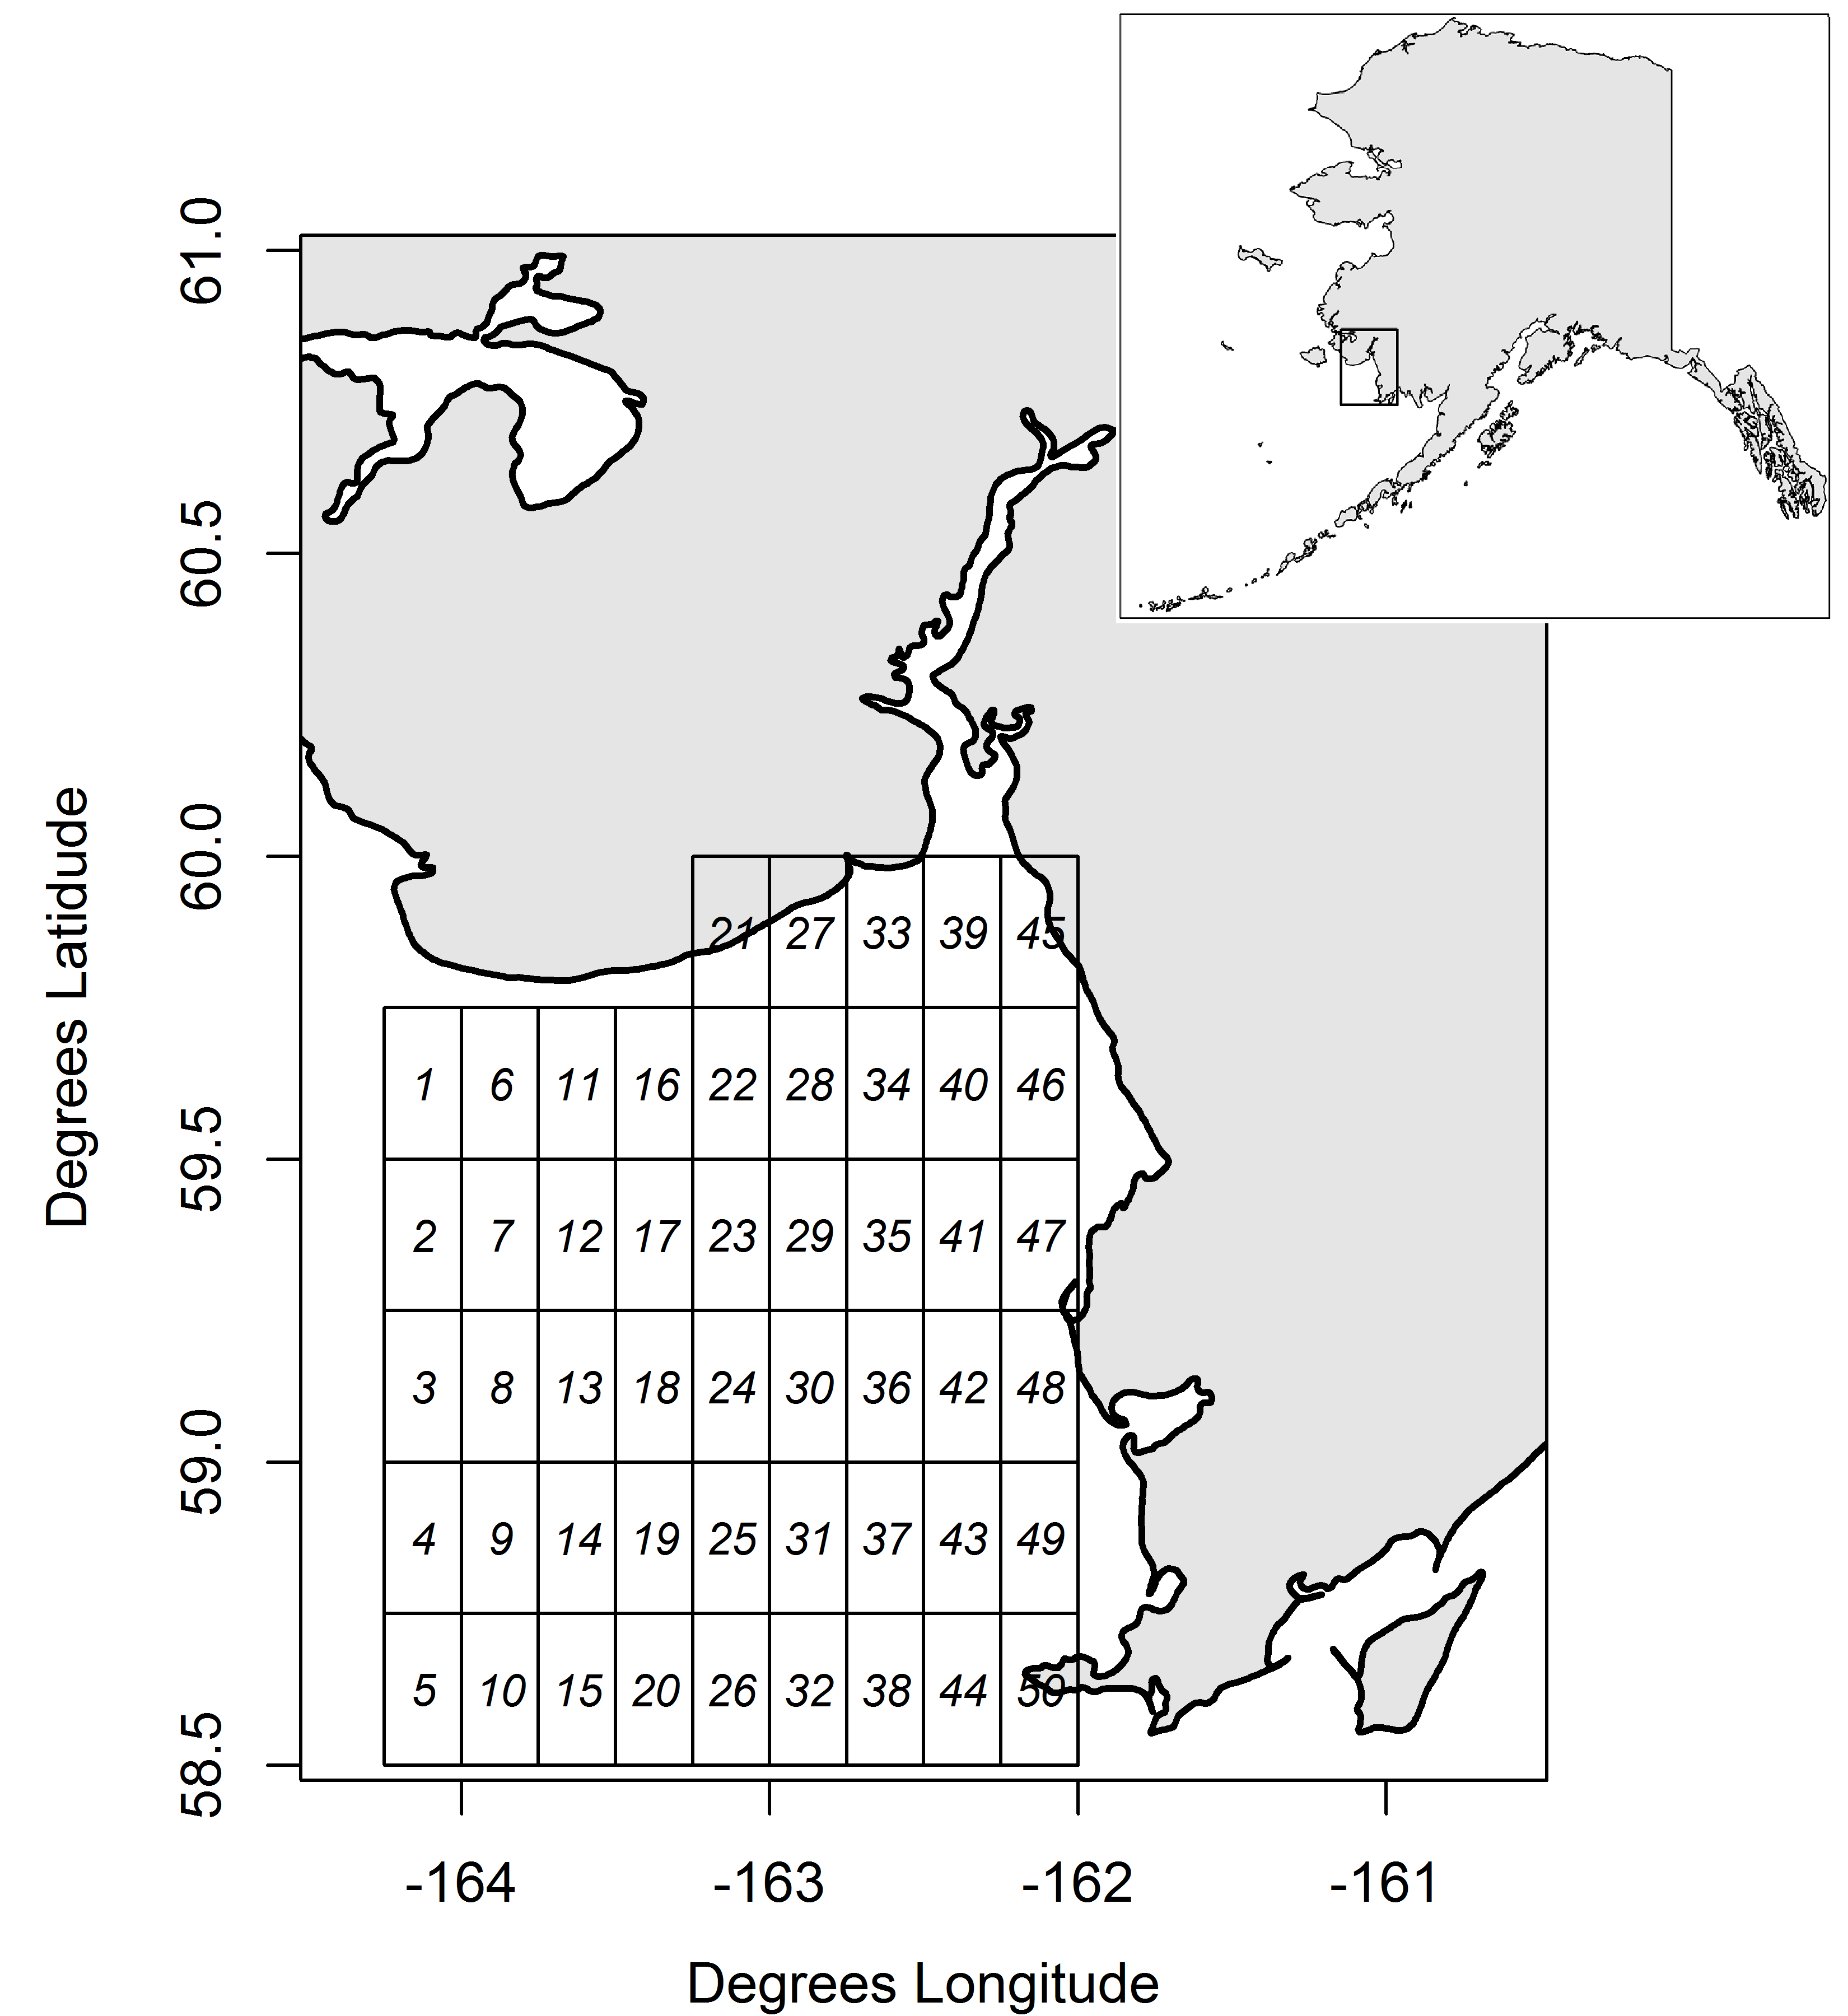
\includegraphics{img/Ch2/map.png}
  \caption{Map of Kuskokwim Bay where Chinook salmon likely stage for transition to freshwater. Shows grid cells from which daily SST values were used. Daily SIC values came from the same grid cells, though excluding grid cell 45 below due to missing values.}
  \label{fig:ch2-map}
\end{figure}

\clearpage

\begin{figure}
  \centering
  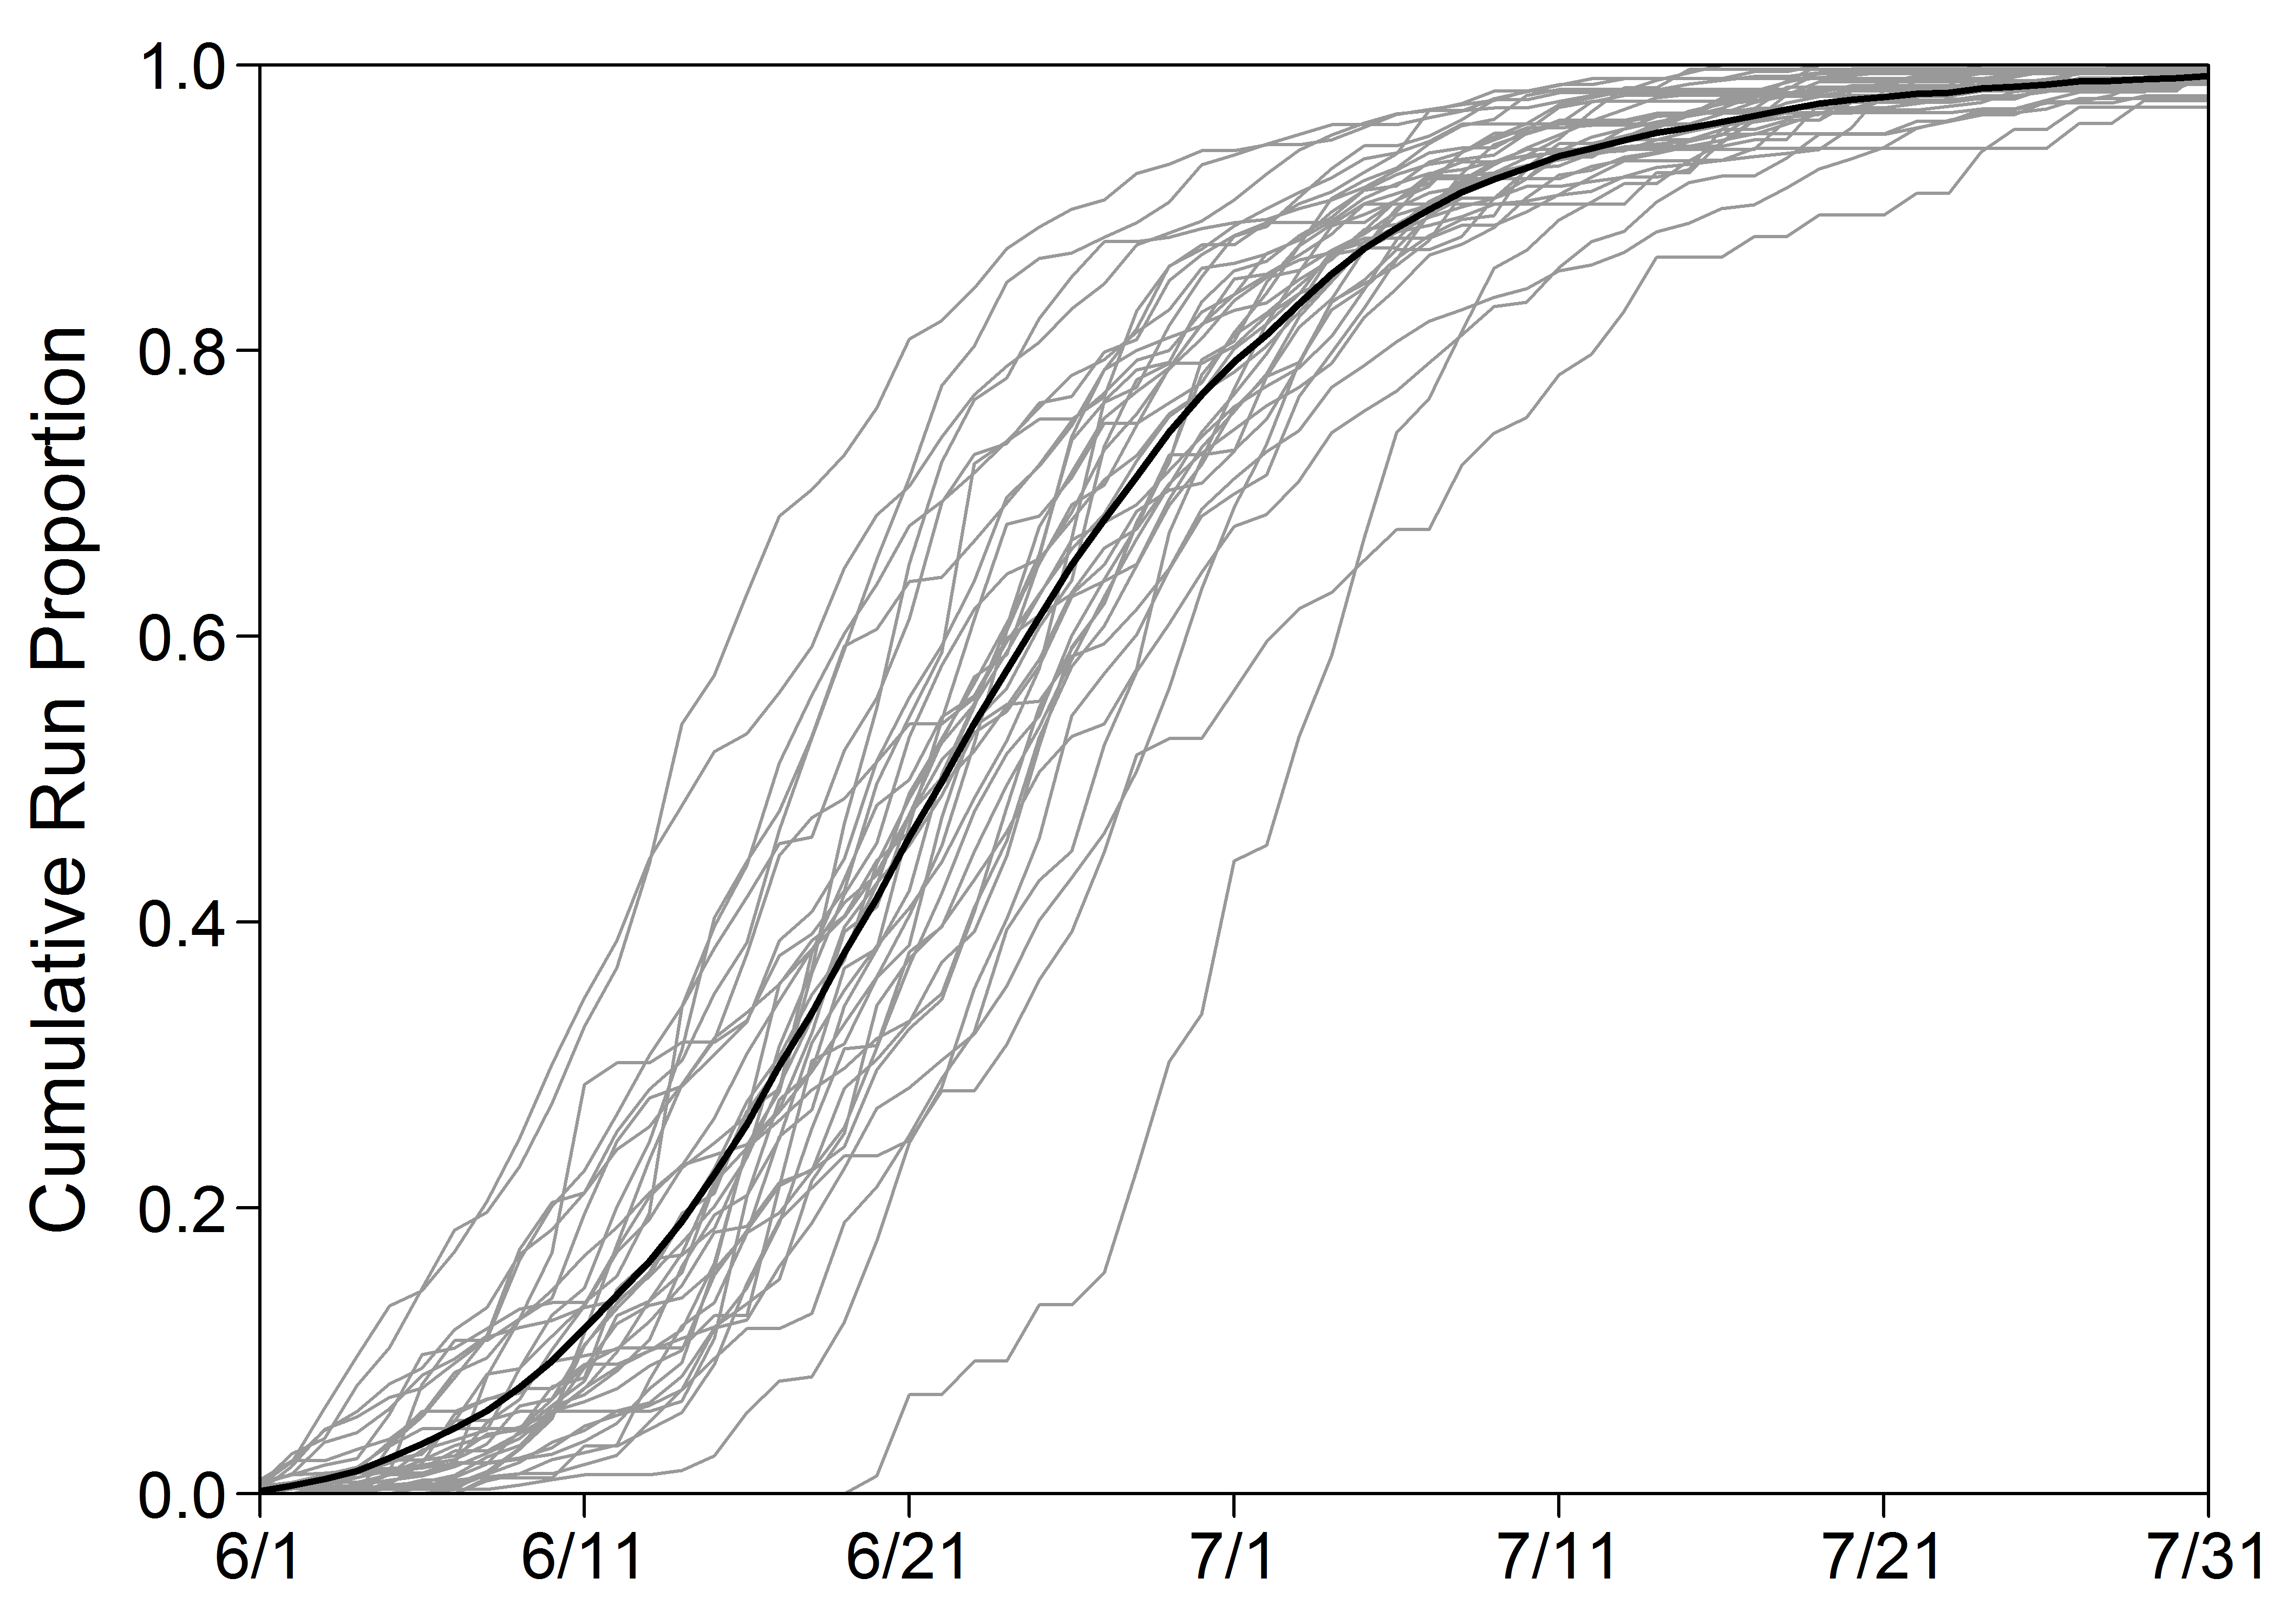
\includegraphics{img/Ch2/p-ccpue.png}
  \caption{Shape and variability of run timing patterns of the Kuskokwim River Chinook salmon stock as sampled by the Bethel Test Fishery, 1984 -- 2018. Each grey curve represents a year standardized by the total end-of-season cumulative CPUE and the black line represents the average value across years on each day of the season.}
  \label{fig:p-ccpue}
\end{figure}

\clearpage

\begin{figure}
  \centering
  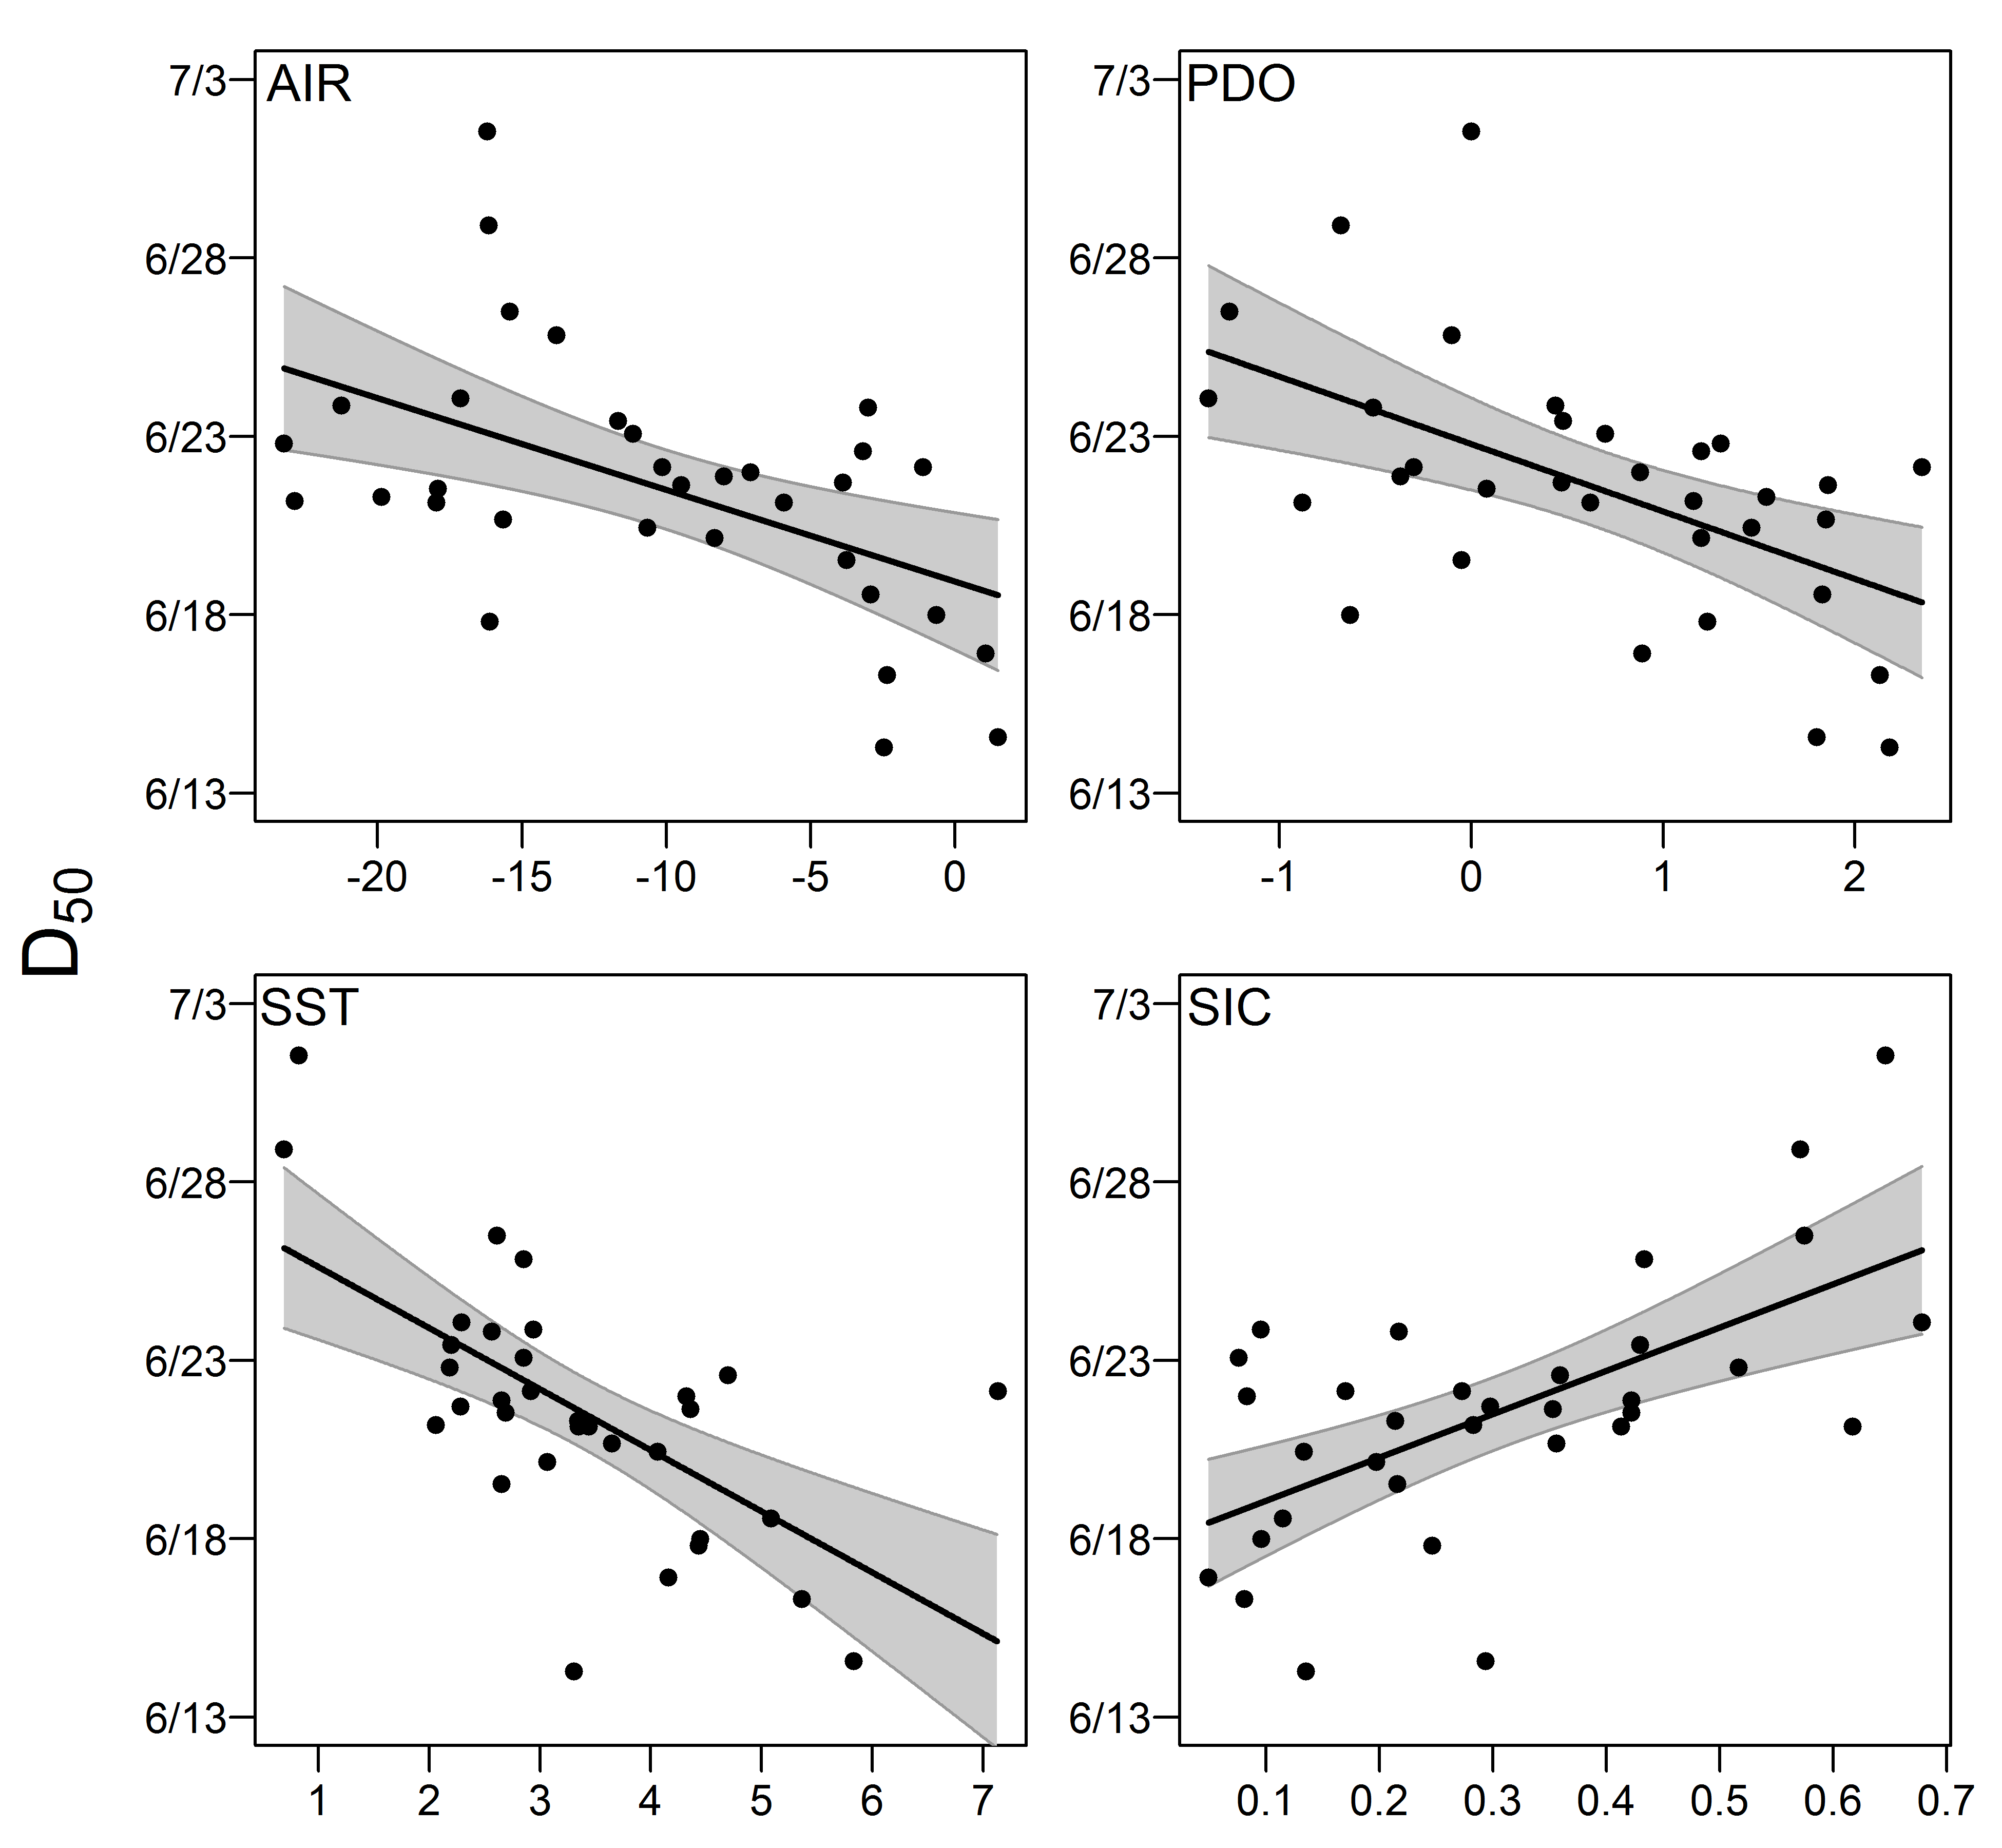
\includegraphics{img/Ch2/relationships.png}
  \caption{Relationships between the four single environmental variables and run timing $\left(D_{50}\right)$ using data from optimal climate windows when 2018 was added to the training data. For illustration purposes only, gridded variables SST and SIC were combined by weighted averaging where the weight of each grid cell was assigned the $\text{AIC}_{\text{c}}$ weight of that grid cell when grid cell-specific models were fit. Grey bands are 95$\%$ confidence intervals on the least squares line.}
  \label{fig:relationships}
\end{figure}

\clearpage

\begin{figure}
  \centering
  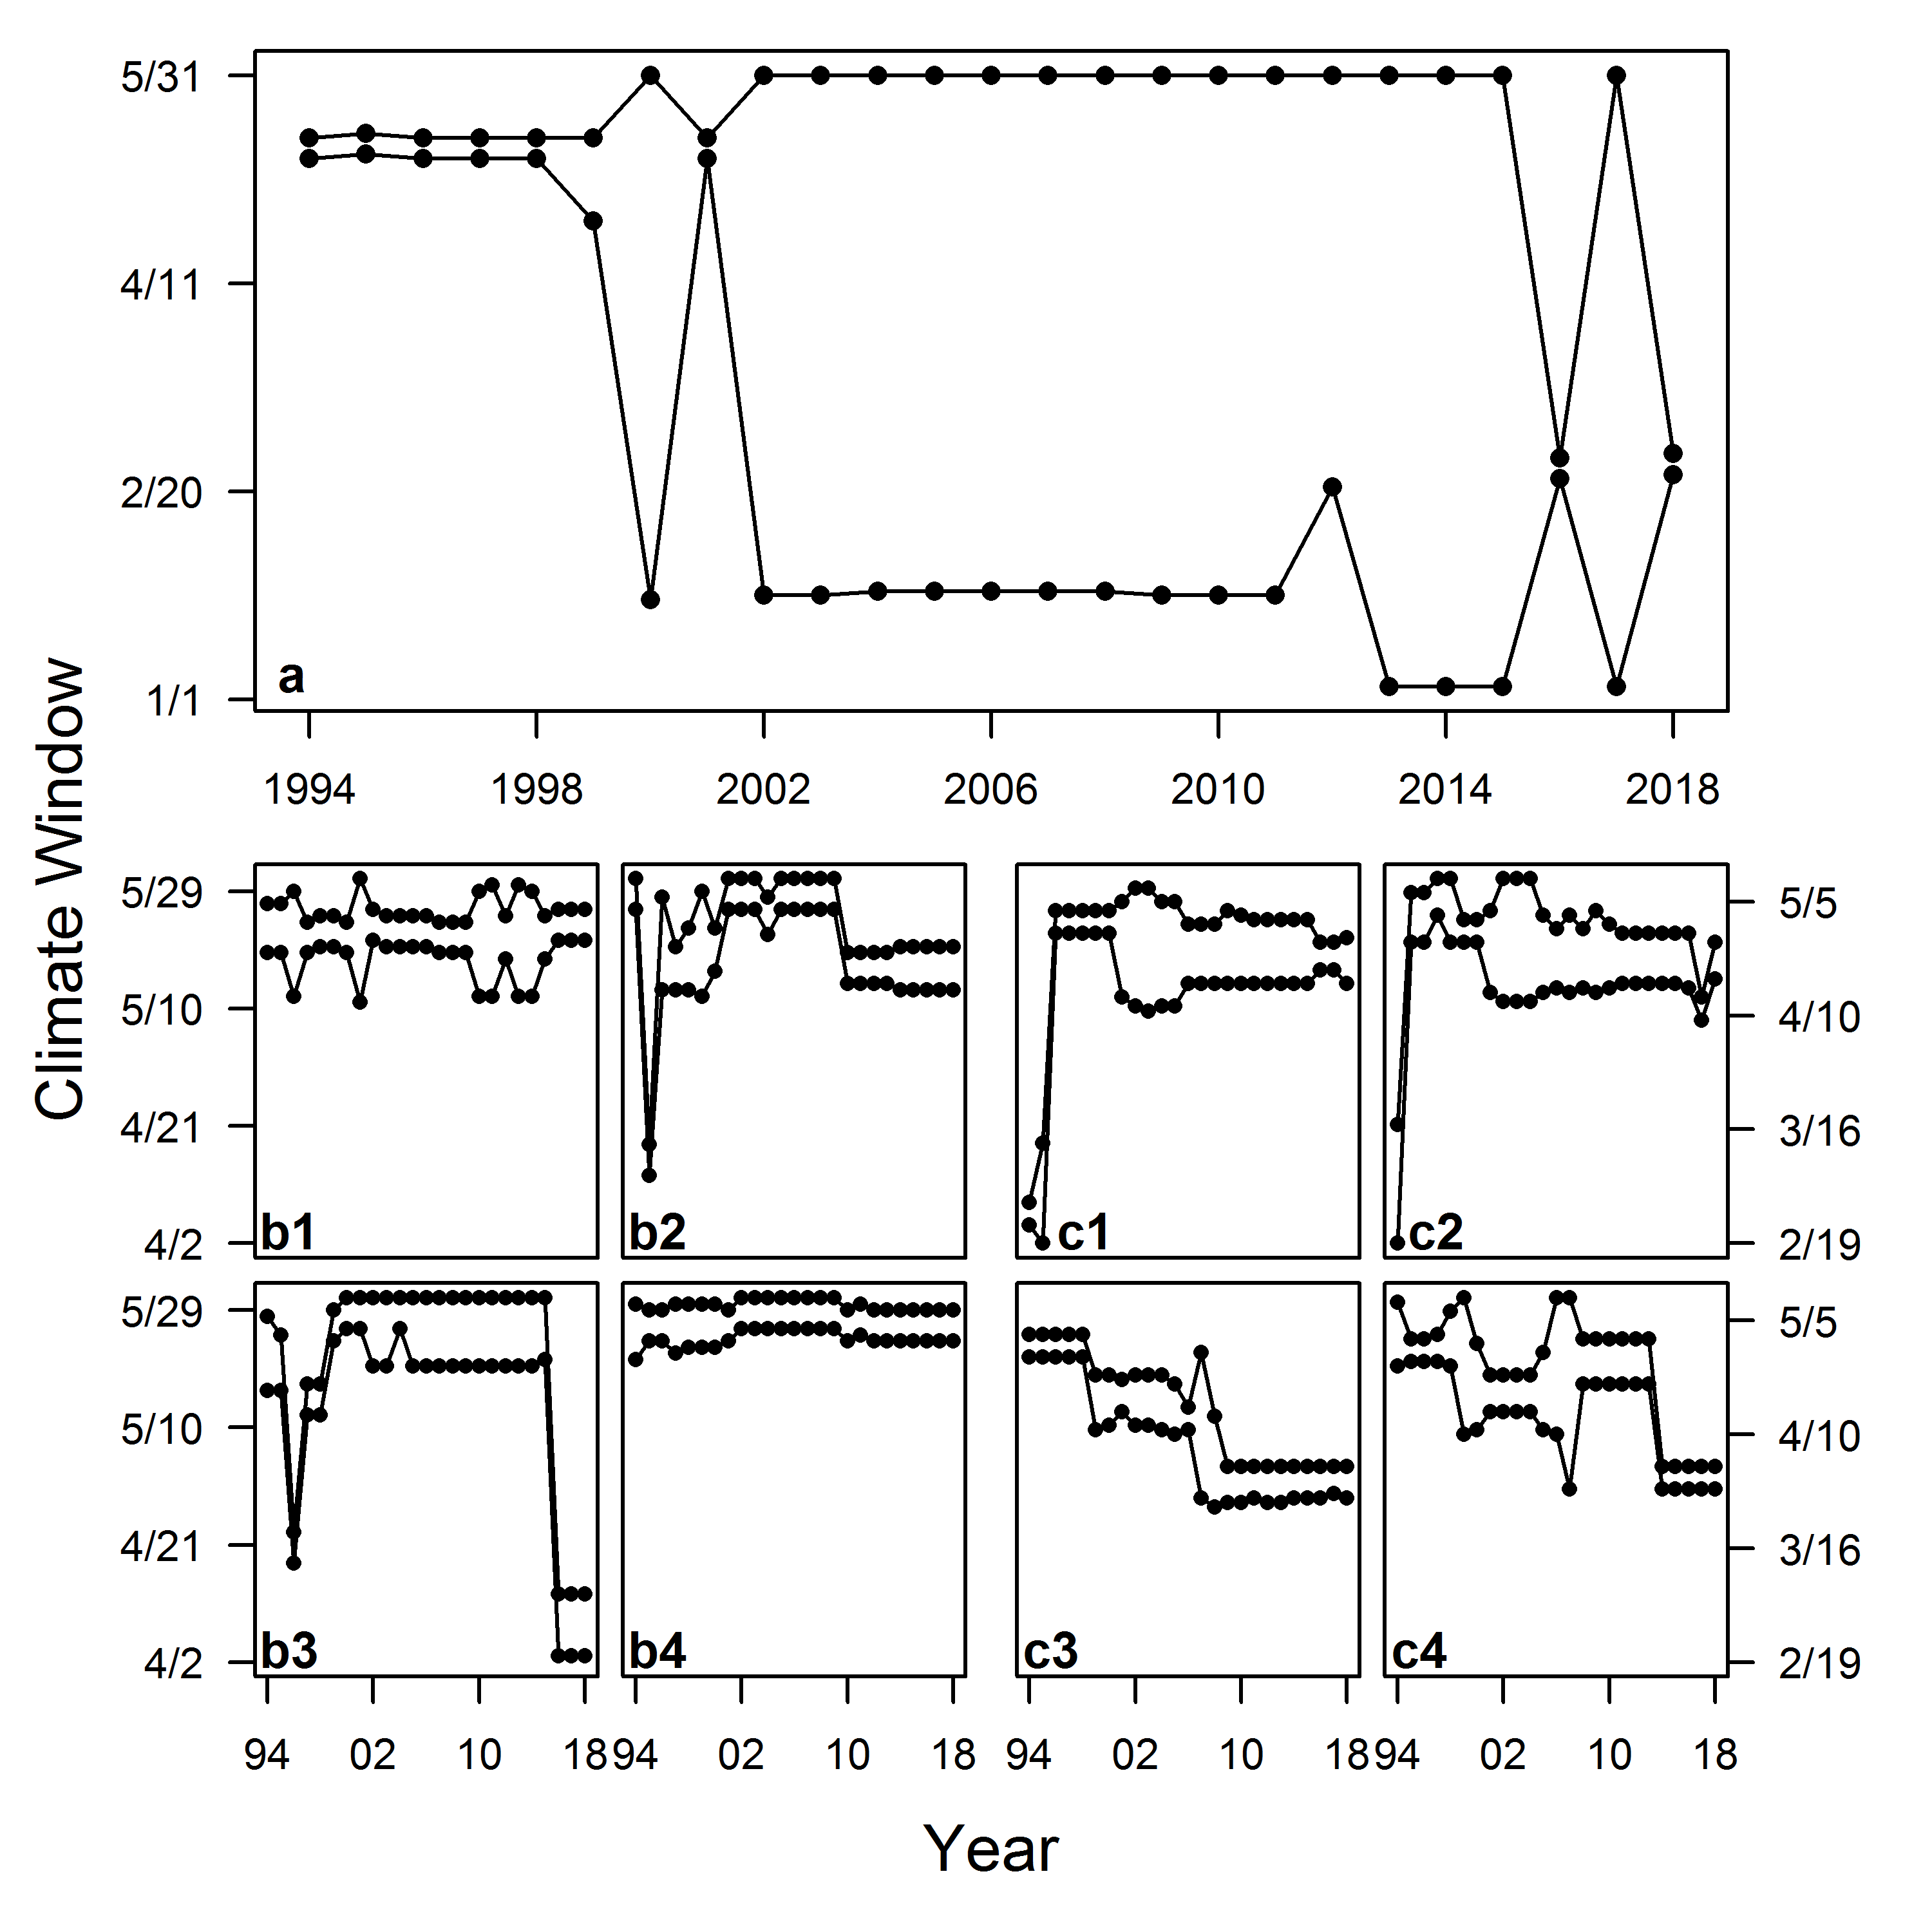
\includegraphics{img/Ch2/window-changes.png}
  \caption{Changes in selected climate windows as training data were added in the retrospective forecasting analysis. Bottom and top lines show the first and last day of the selected climate window, respectively, as more years were added. The year axis corresponds to the selected window after including environmental and run timing data from that year in the training data. E.g., the windows shown for 2017 were used to produce the forecast for 2018. Panel (\textit{a}) is Bethel air temperature, panels \textit{b}1 -- \textit{b}4 are SST windows for four sample grid cells and panels c1-c4 are SIC windows for the same four sample grid cells. Sample grid cells from Figure \ref{fig:ch2-map} shown for SST and SIC are as follows: grid cell 8 (\textit{b}1, \textit{c}1), grid cell 44 (\textit{b}2, \textit{c}2), grid cell 12 (\textit{b}3, \textit{c}3), and grid cell 48 (\textit{b}4, \textit{c}4). Selected windows for PDO are not shown because the single month of May was selected in all years.}
  \label{fig:window-changes}
\end{figure}

\clearpage

\begin{figure}
  \centering
  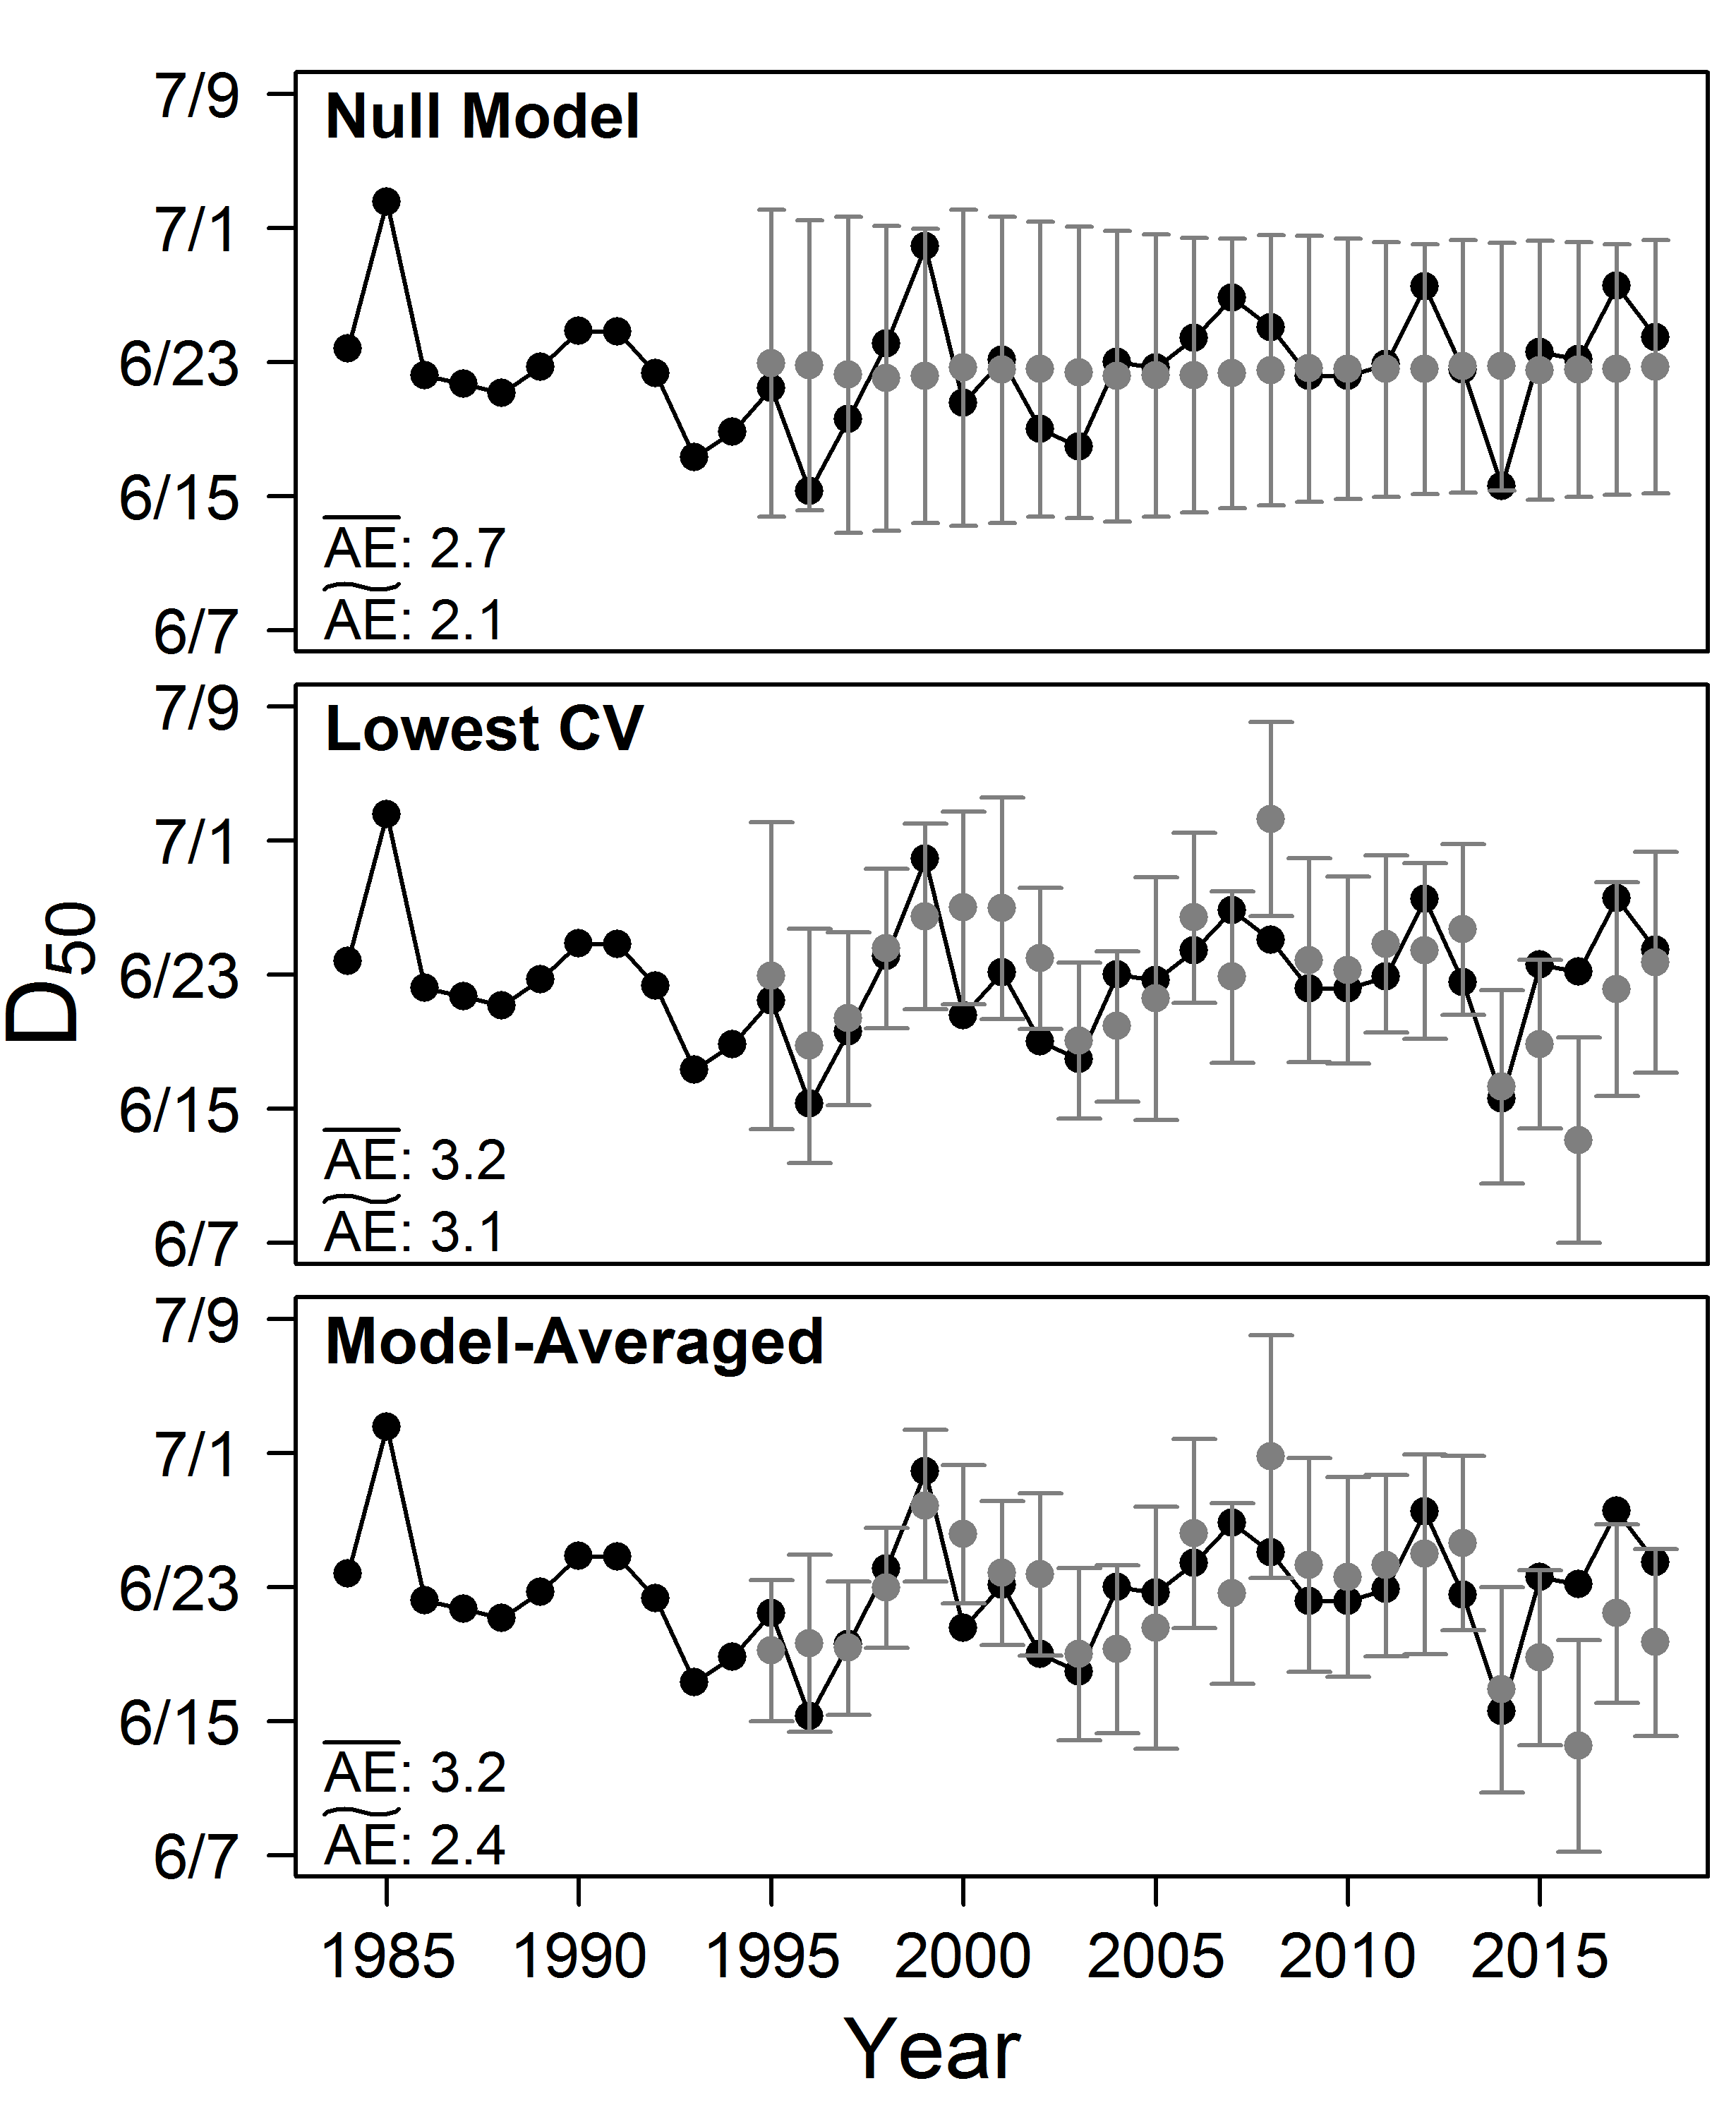
\includegraphics{img/Ch2/forecasts.png}
  \caption{Produced forecasts under the three approaches. Black points/lines are the time series of $D_{50}$ detected by the BTF. Grey points are out-of-sample forecasts with 95$\%$ prediction intervals shown as error bars. $\overline{\text{AE}}$ and $\widetilde{\text{AE}}$ are the mean and median absolute forecast errors from 1995 to 2018, respectively.}
  \label{fig:forecasts}
\end{figure}

\clearpage

\begin{figure}
  \centering
  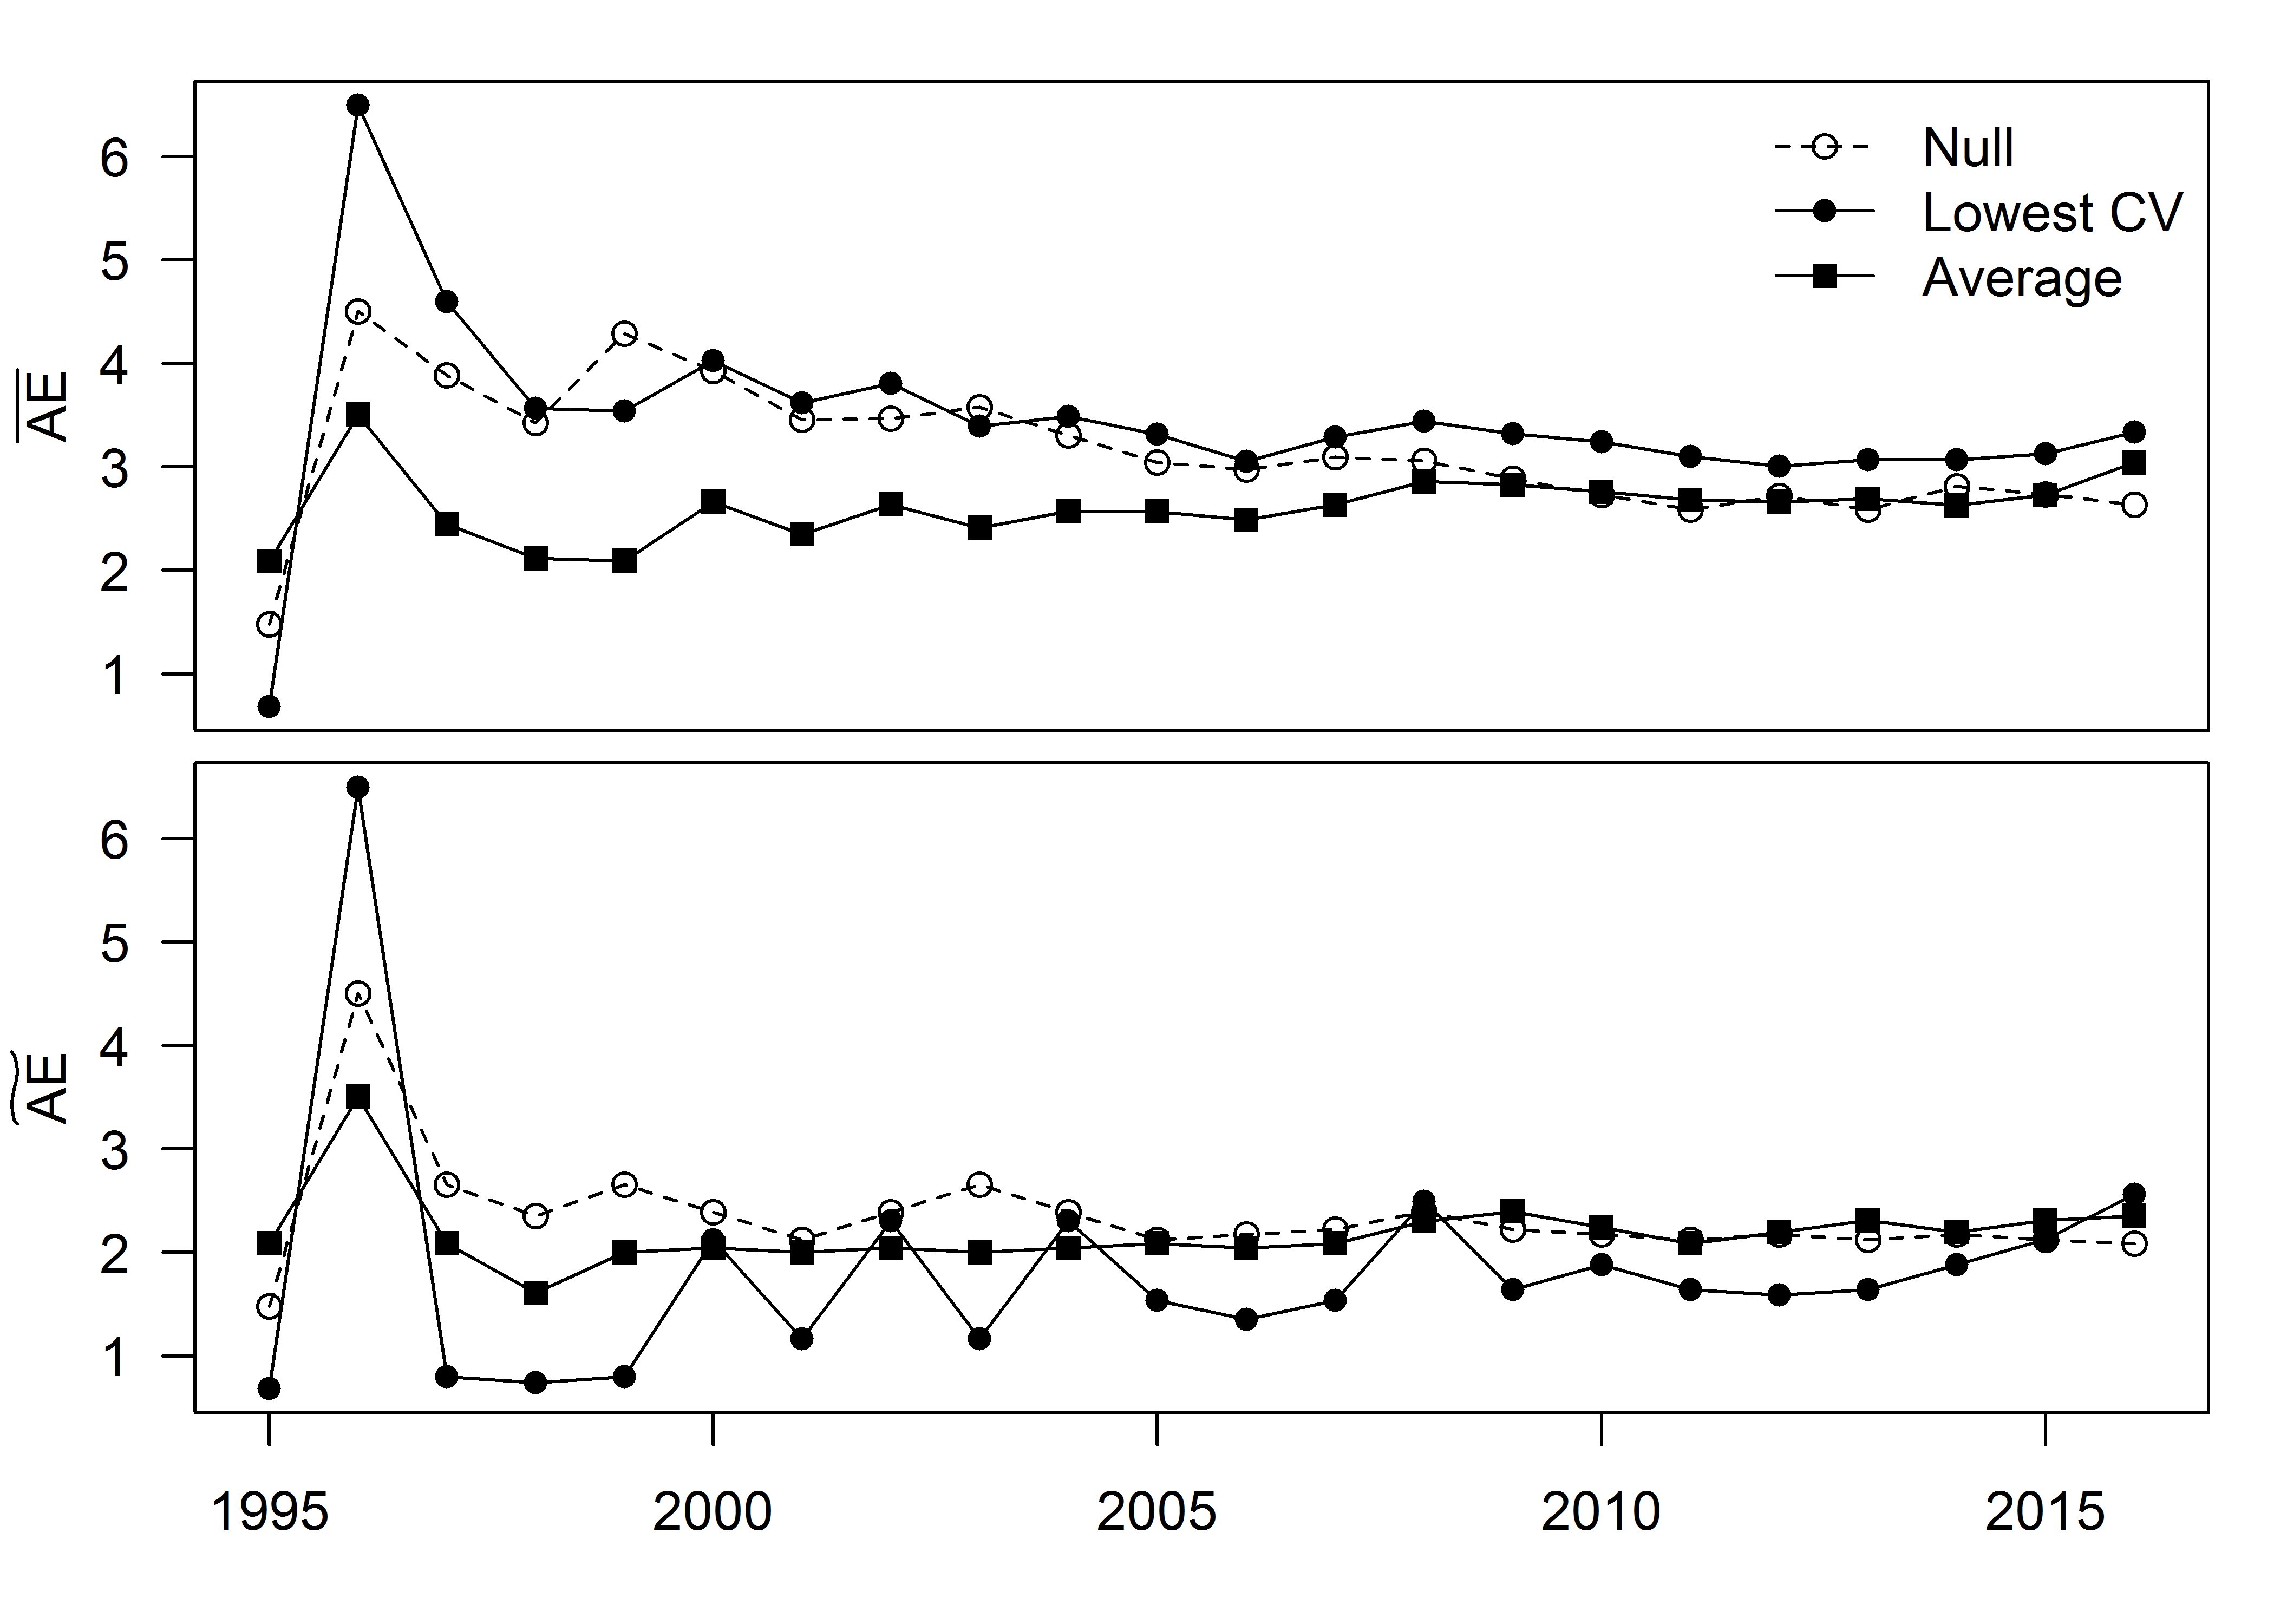
\includegraphics{img/Ch2/ae-changes.png}
  \caption{Evolution of $\overline{\text{AE}}$ (mean) and  $\overline{\text{AE}}$ (median) absolute forecast error under the three investigated forecasting approaches. Each point is the average of absolute errors of all years before and including the corresponding year on the $x$-axis, starting in 1995.}
  \label{fig:ae-changes}
\end{figure}

\clearpage

\begin{figure}
  \centering
  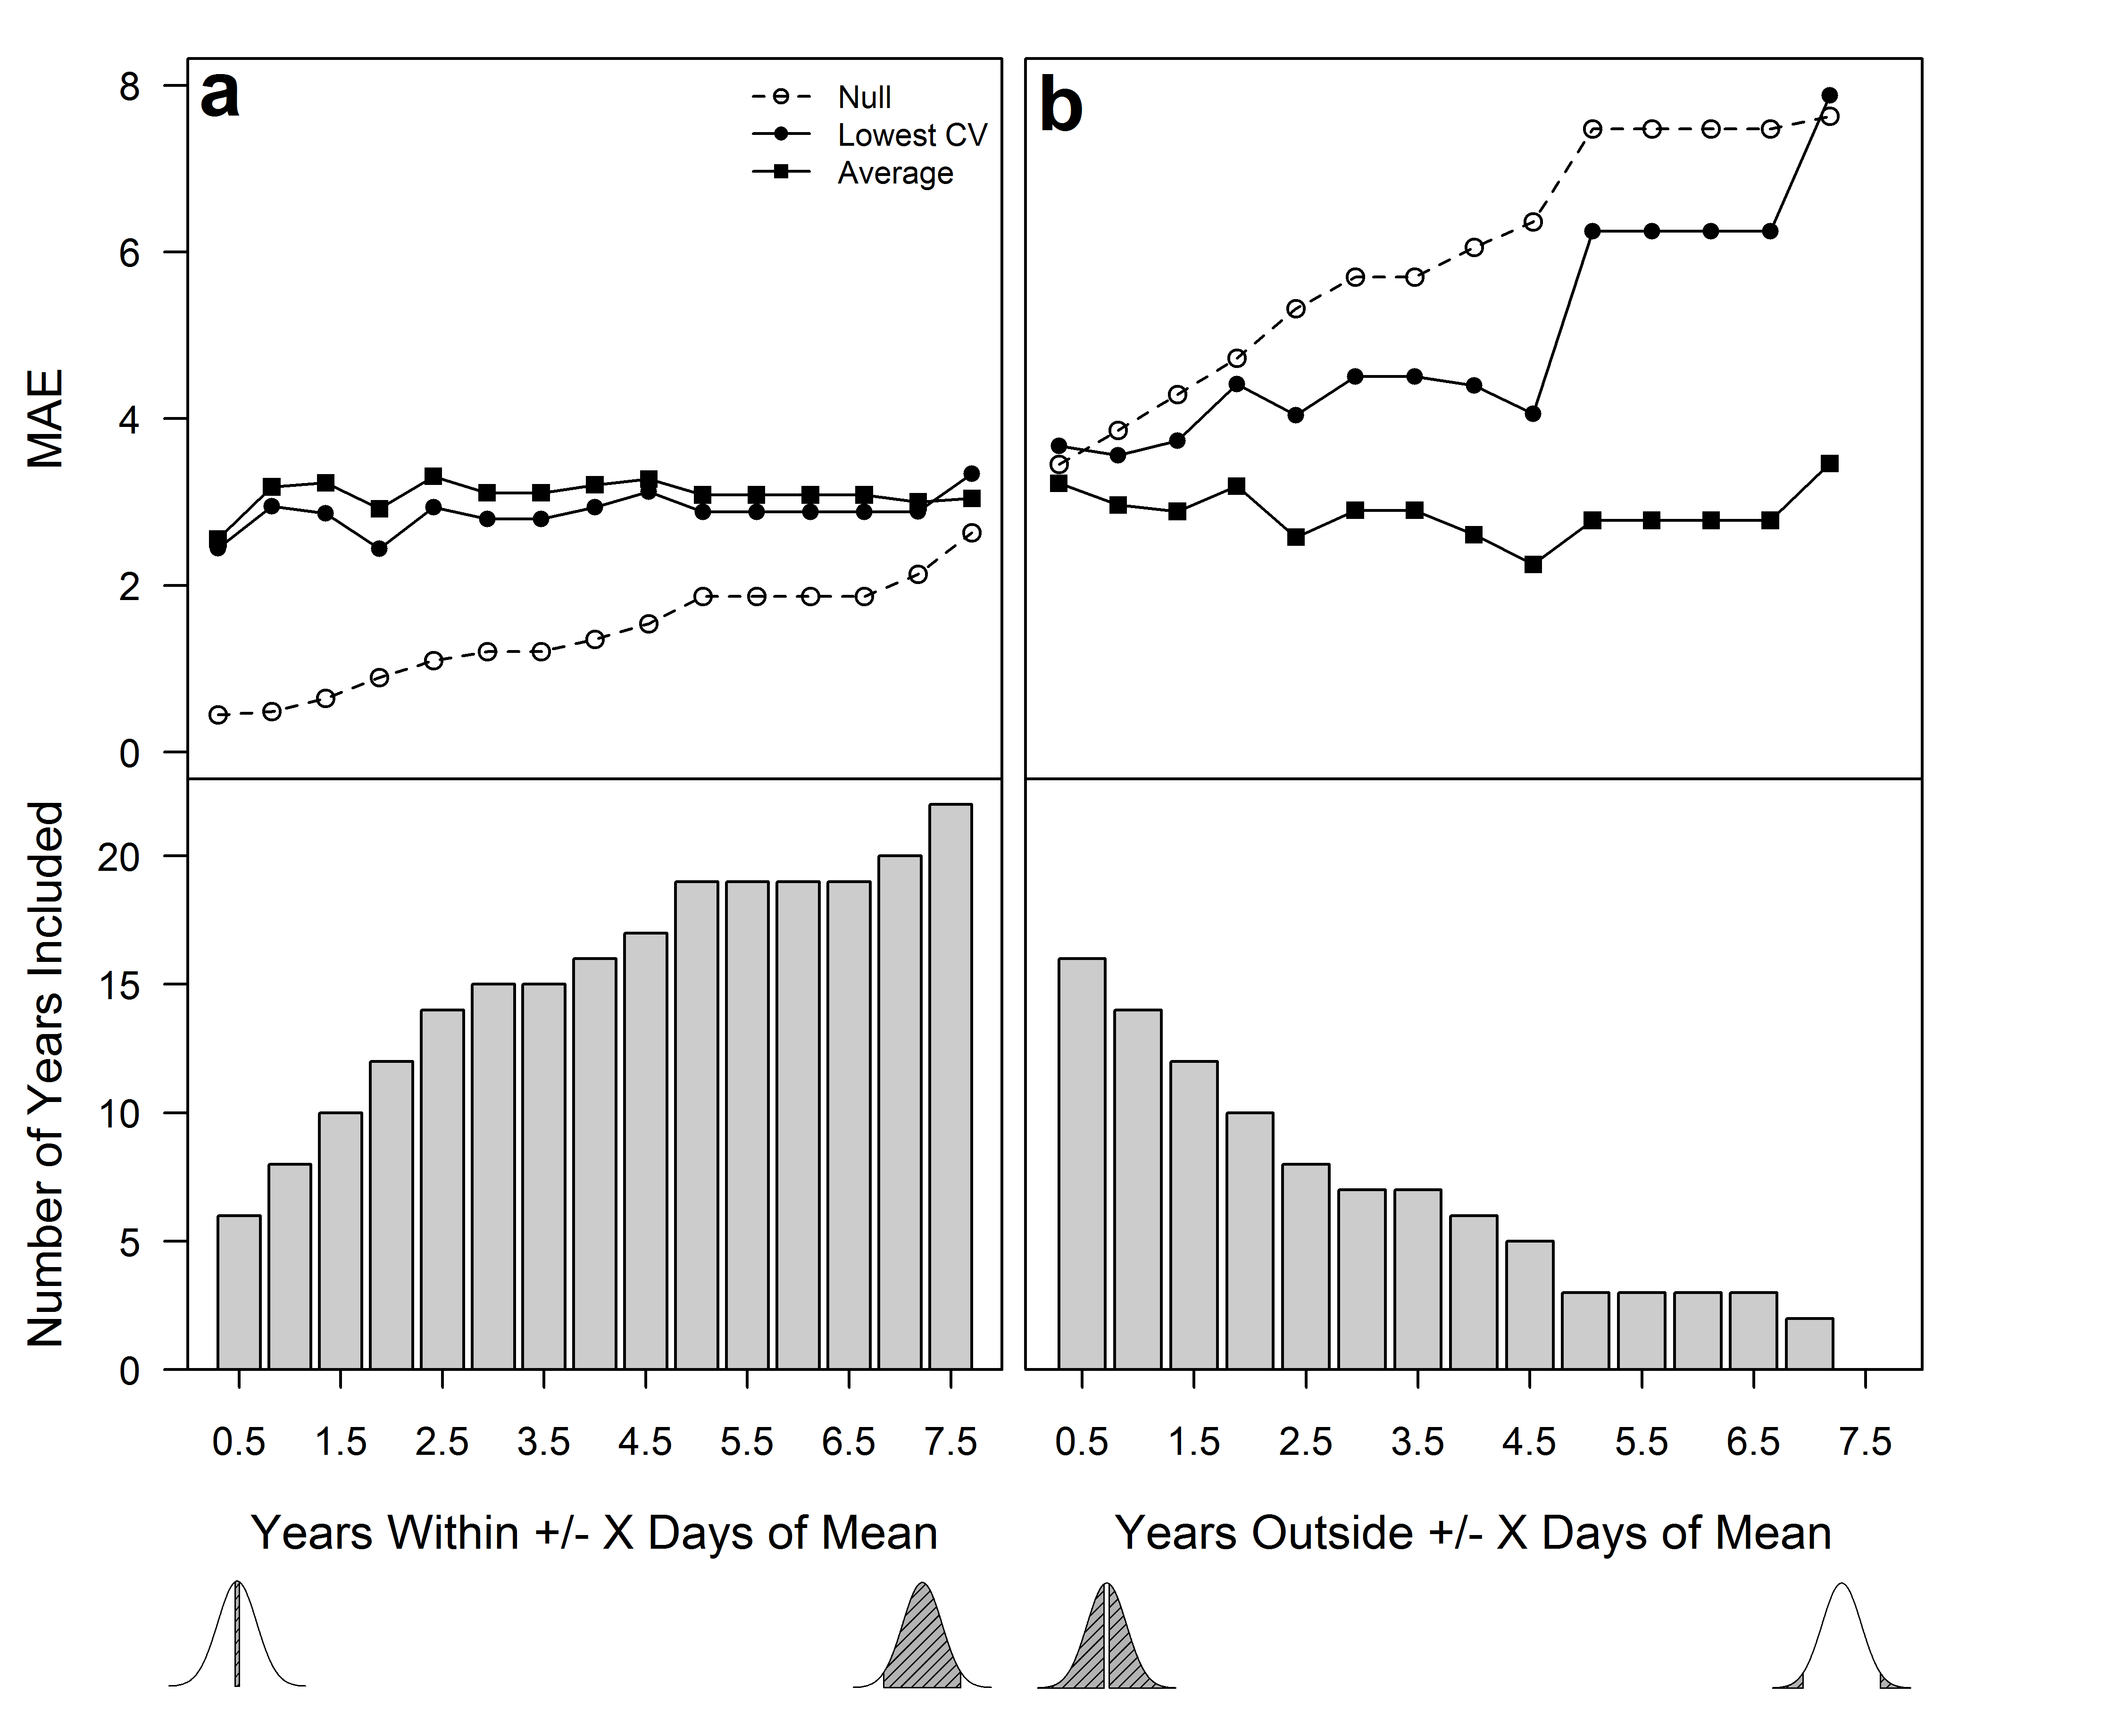
\includegraphics{img/Ch2/mae-subsets.png}
  \caption{$\overline{\text{AE}}$ under three forecast approaches calculated by either (\textit{a}) including years with a $D_{50}$ value within $\pm x$  days of the all-year average or (\textit{b}) including years with a $D_{50}$ value outside $\pm x$ days of average, where $x$ is the number of days indicated on the $x$-axis. Bottom panels show the number of observed years in which the appropriate $\pm x$ days criterion was met. Shaded regions in the hypothetical distributions show the types of $D_{50}$ values that were included in the calculation of $\overline{\text{AE}}$. One point that may enrich inference from this figure (and is shown in the shaded normal distributions) is that panel (\textit{a}) becomes more inclusive from left to right by adding years that are more dissimilar to the average in the calculation of $\overline{\text{AE}}$ whereas panel (\textit{b}) becomes more exclusive from left to right by removing years that are similar to the average.}
  \label{fig:mae-subsets}
\end{figure}

\clearpage

\begin{figure}
  \centering
  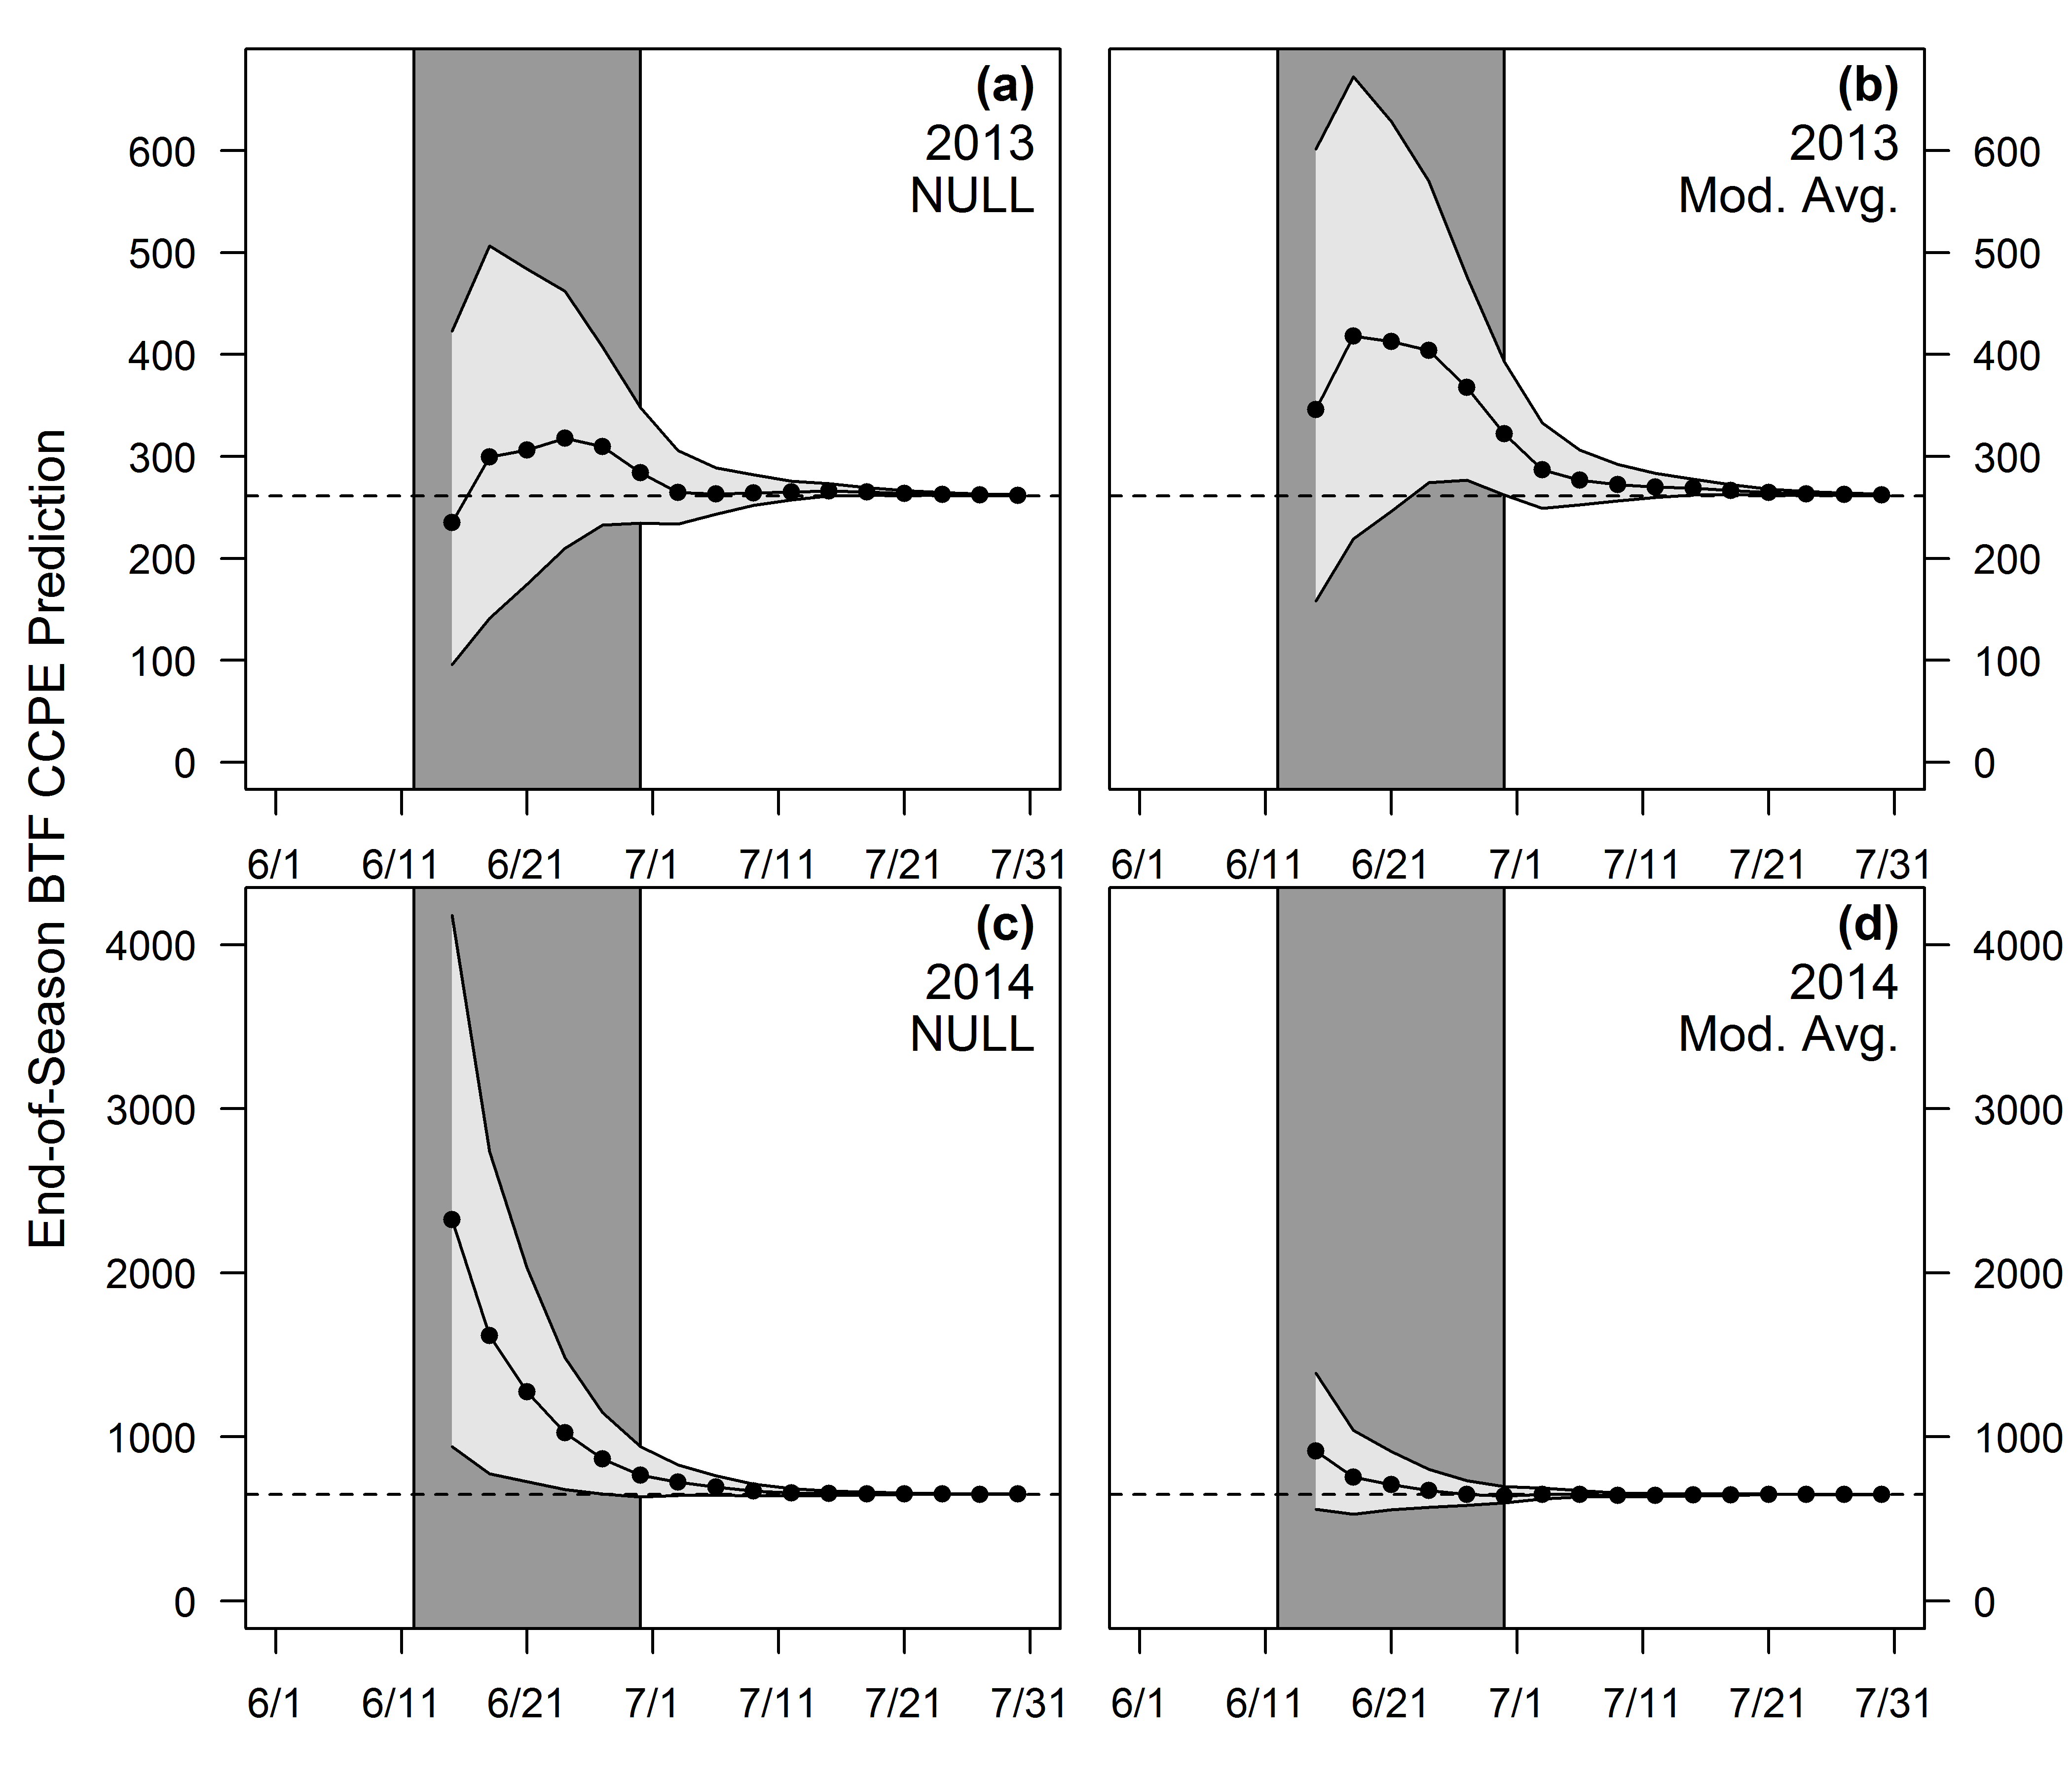
\includegraphics{img/Ch2/eos-preds.png}
  \caption{In-season predictions of end of season cumulative BTF CPUE under the model-averaged forecast using environmental variables and the forecast under the null model in 2013 and 2014. Intended to illustrate cases in which a manager would benefit from having access to the model-averaged run timing forecast model using environmental variables (2014) and when the null model would have performed better (2013). Horizontal lines are the true end of season cumulative BTF CPUE, dark grey regions are 50$\%$ confidence intervals, and light grey regions are 95$\%$ confidence intervals. Grey vertical lines indicate the period when key harvest decisions are made.}
  \label{fig:eos-preds}
\end{figure}

\begin{figure}
  \centering
  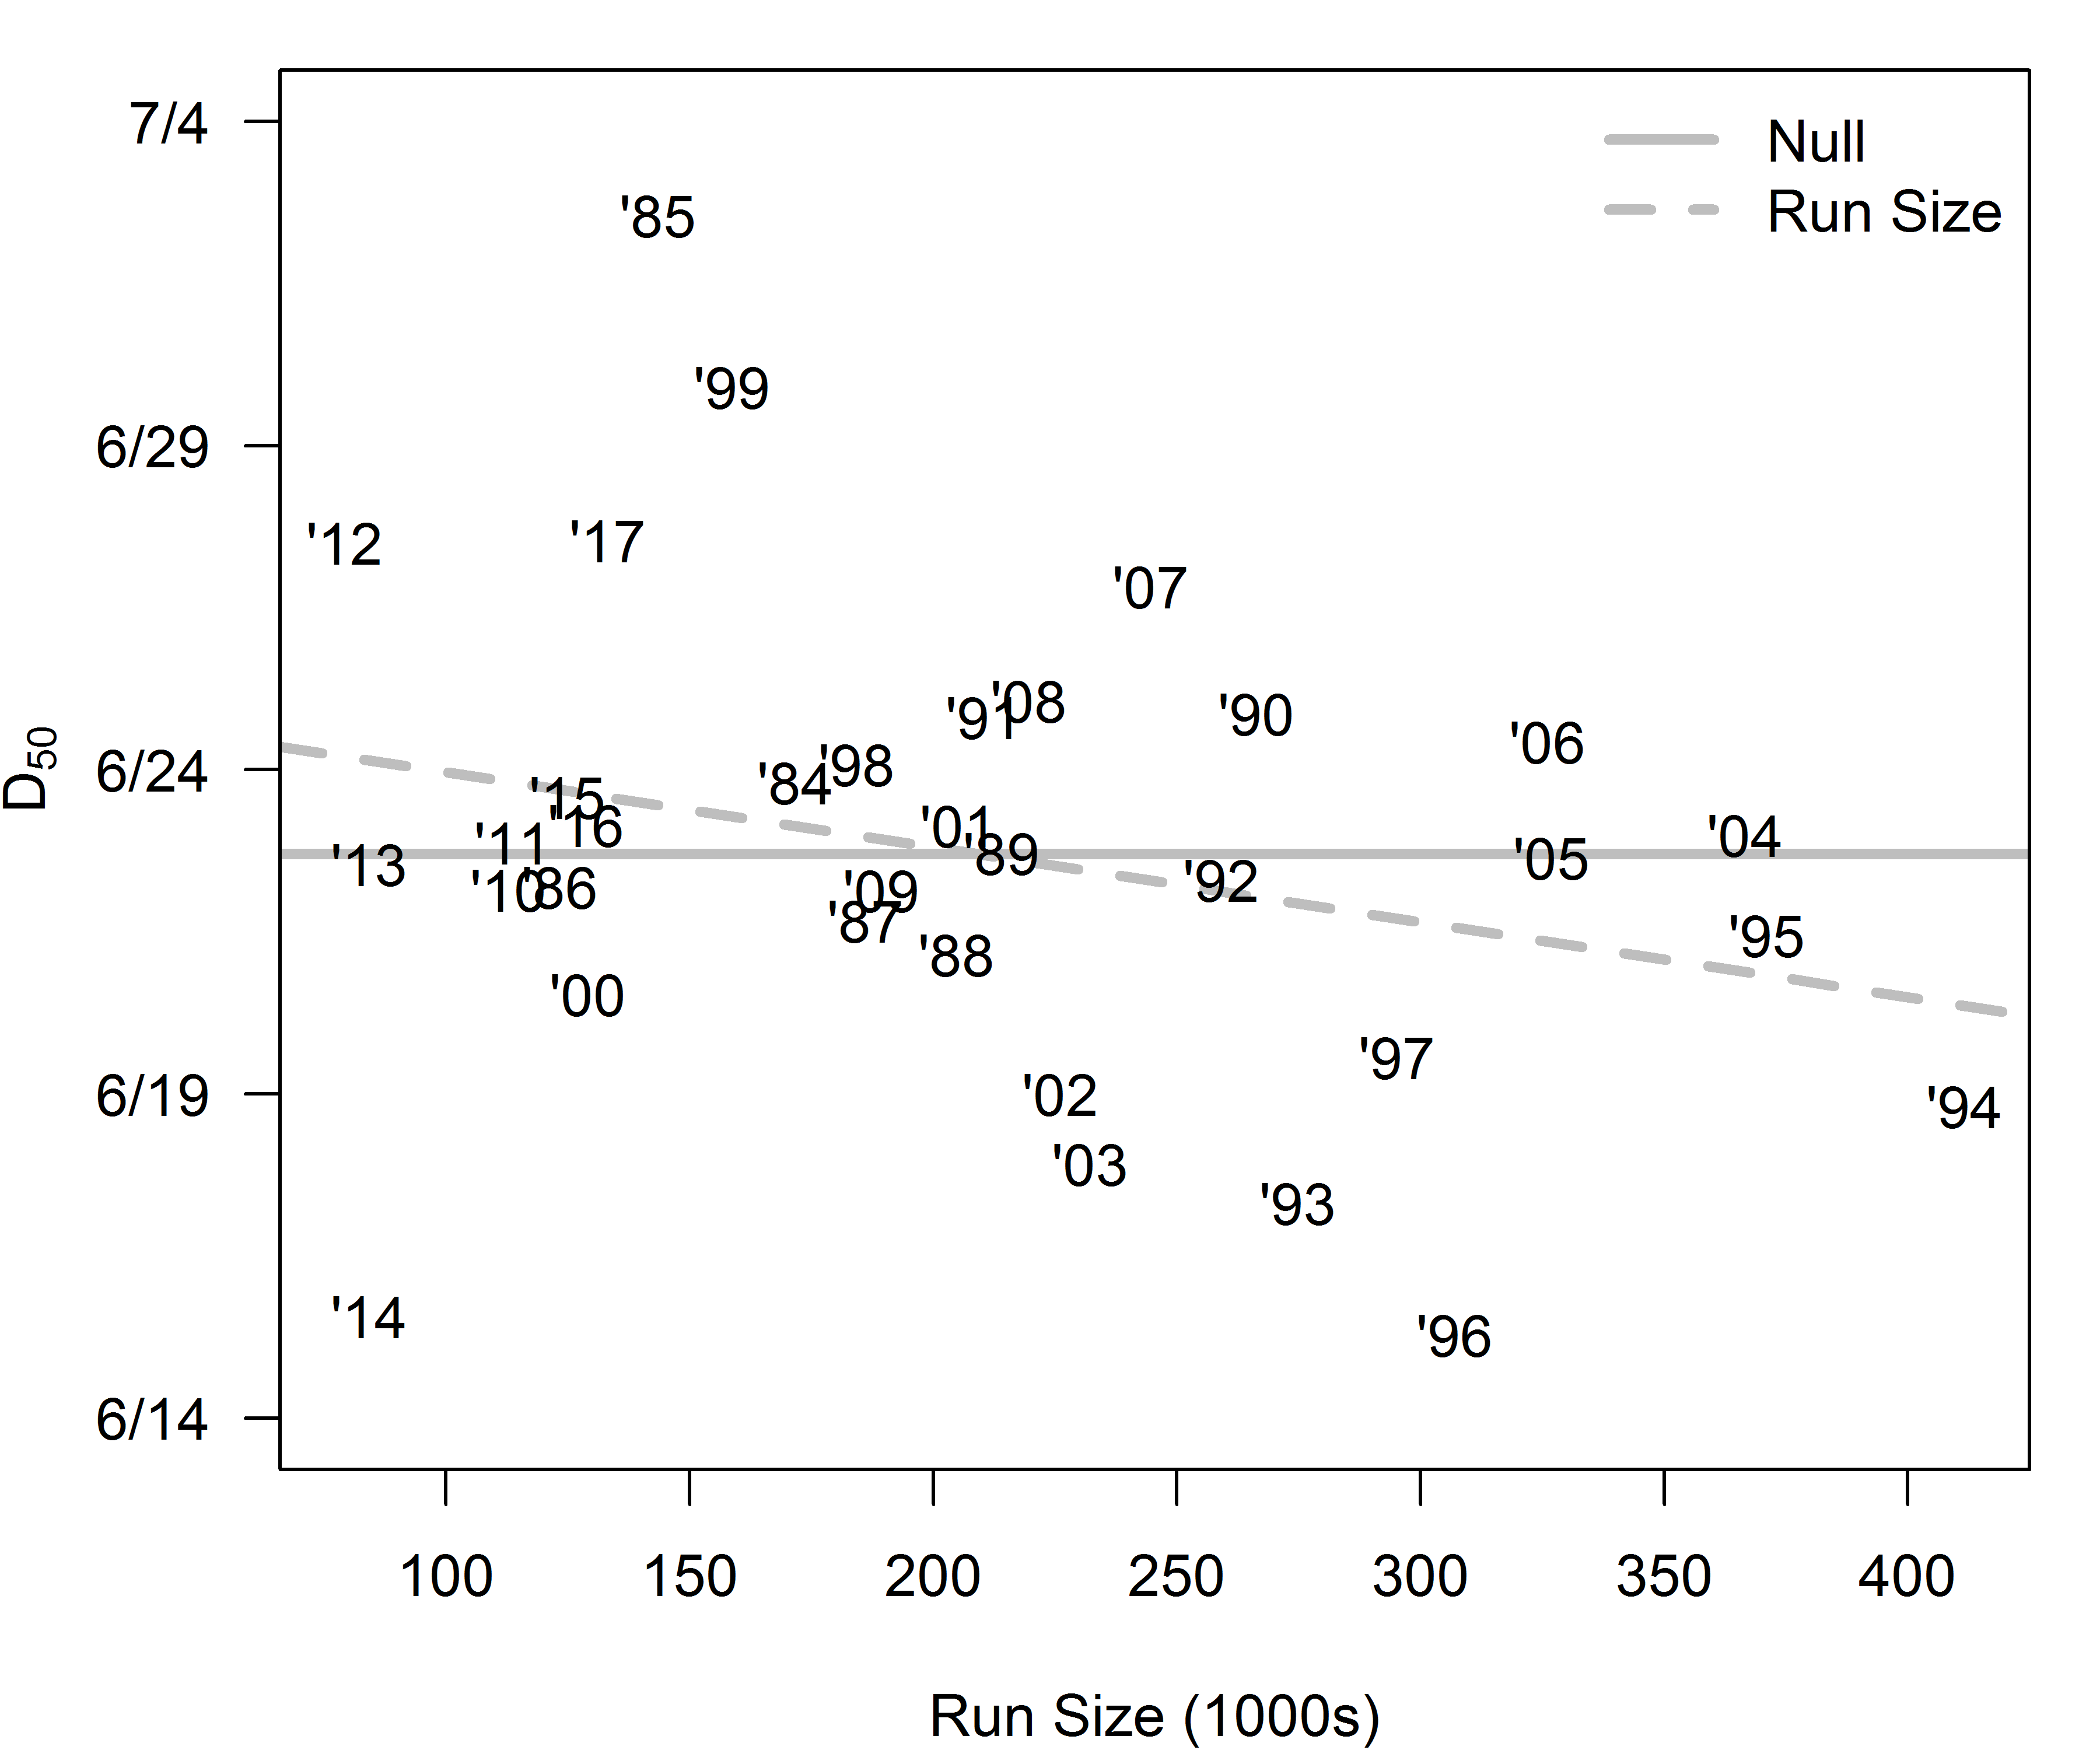
\includegraphics{img/Ch2/rt-n.png}
  \caption{Relationship between $D_{50}$ and run size for Kuskokwim River Chinook salmon with two fitted models shown: the null model (which assumed constant mean $D_{50}$) and the run size model (which assumed the mean $D_{50}$ changes as a function of run size). As described in the text, the effect of run size on run timing was very small and not significantly different than no effect. Additionally, knowledge of run size did not result in smaller average prediction errors of $D_{50}$ than not having this knowledge.}
  \label{fig:rt-n}
\end{figure}

\chapter{Evaluation of In-Season Harvest Management Strategies For
Kuskokwim River Chinook Salmon using a Stochastic Simulation
Model}\label{ch3}

\section*{Abstract}\label{abstract-1}
\addcontentsline{toc}{section}{Abstract}

\noindent
In-season management of Chinook salmon subsistence fisheries in large
river basins is conducted in the presence of much uncertainty, primarily
with respect to run size and timing. Managers must manipulate the amount
of time in which fishing is allowed to ensure adequate escapement to
sustain future harvests while simultaneously providing as much
opportunity in the current year as possible. In doing so, they may use a
set of decision rules to open or close the fishery based on either
intuition or assessment information. Inferences about which strategies
may perform better in certain circumstances can be informed using
management strategy evaluation, an analytical method in which decision
rules and information sources are tested against simulated conditions to
measure likely management performance. I conducted a management strategy
evaluation for in-season harvest management for the Kuskokwim River
Chinook salmon subsistence fishery in western Alaska to test four
primary management strategies that ranged in their complexity and
information needs. Findings showed that all assessed strategies can
perform well, but that the more complex strategies tended to perform
better when the incoming run was small. Additionally, the optimal
settings (i.e., aggressive or conservative with respect to fishing
opportunity) of each strategy depended on run size, with conservative
settings favored in smaller runs. The findings of this chapter extend
the knowledge about in-season salmon harvest management strategies,
which is mostly regarding commercial fisheries, to include subsistence
fisheries as well and should be informative to fishery managers in the
region.

\newpage

\section{Introduction}\label{introduction-1}

\noindent
In-season harvest management of Pacific salmon (\emph{Oncorhynchus}
spp.) fisheries in large river systems is undertaken in the presence of
a large amount of uncertainty about how to schedule fishing
opportunities. In order to manage in a fully-informed way, a manager
would require continuous and accurate information on arrival timing, run
size, fleet dynamics, and harvest. With knowledge on these components,
it would be theoretically possible to perfectly harvest the available
surplus each year \citep{adkison-cunningham-2015}. In reality, these
quantities (when available) are often highly uncertain
\citep{adkison-peterman-2000, flynn-hilborn-2004, hyun-etal-2012} which
results in difficulties in decision-making about how to best implement
the fishery in order to meet a set of pre-defined objectives dealing
with both conservation and exploitation.

In addition to the substantial uncertainty in decision-making, there are
often sharp trade-offs between competing objectives, such as the desire
to provide adequate and equitable harvest opportunity \emph{versus} the
desire to ensure adequate escapement \citep{catalano-jones-2014}.
Oftentimes, managers are also concerned with spreading exploitation
evenly among stock subcomponents \citep{schindler-etal-2010}, but this
may conflict with aspects dealing with the ideal time to harvest salmon
as a result of weather or fish quality conditions
\citep{carney-adkison-2014b, adkison-cunningham-2015}. When given the
task of balancing trade-offs such as these, the manager has the ability
to manipulate the fishing gear used as well as the spatiotemporal
distribution of fishing effort by opening or closing the fishery for
various amounts of time, though it is rarely clear as to how to
manipulate these management ``levers'' to achieve the desired outcomes.
Presumably, different strategies to performing these manipulations
(termed ``management strategies'') will exhibit differential performance
at meeting the objectives and balancing trade-offs.

Management strategy evaluation (MSE) has been proposed as a powerful
tool for determining how to manage exploited natural resource systems
with competing management objectives
\citep{cooke-1999, butterworth-2007}. MSE is a stochastic
simulation-based analytical technique whereby management strategies are
evaluated by comparing their relative performance at meeting pre-defined
objectives under simulated (though realistic) conditions. A management
strategy can be thought of as all of the steps that encompass the
collection of data, subsequent analyses, and resulting decision-making
surrounding the exploitation of a resource. The MSE approach tests a
range of such strategies to find the one(s) that are likely to be most
robust to uncertainty and balance trade-offs. This approach is powerful
as it can provide general insights without having to test strategies on
the real system, which would be incredibly time-intensive (each year is
one sample) and costly given that some candidate strategies can be risky
\citep{walters-martell-2004}. \citet{punt-etal-2014} outlined a set of 7
steps to an MSE that must be conducted in order for the analysis to be
meaningful:

\begin{enumerate}
\def\labelenumi{(\arabic{enumi})}
\item
  identification of management objectives and performance measures for
  each; preferably under the direction of stakeholders and managers,
\item
  identification of the key uncertainties present in the system
  (biological, assessment, implementation, etc.),
\item
  identification of candidate management strategies for evaluation,
\item
  development of one or more models that serve as the representation of
  the real system including reasonably realistic representations of
  biological and fishery components (termed the ``operating model''),
\item
  selection of parameters to drive the operating model in accordance
  with the real system,
\item
  simulation of executing each strategy using the operating model(s),
  and
\item
  summary of performance measures, and presentation to managers and
  stakeholders.
\end{enumerate}

Two broad classes of strategies could be conceived for in-season salmon
management: effort control using either (1) a fixed schedule set at the
start of the season or (2) a feedback strategy where the fishery is
opened or closed in response to in-season data \citep[i.e., management
by emergency order,][]{adkison-cunningham-2015}. There exist many
substrategies that fall into these two broad categories based on (1) the
level of risk aversion on the part of the manager (i.e., aggressive
\emph{versus} conservative) and (2) the timeliness and reliability of
information available to the manager. In general, more complex
strategies will require more data to inform their implementation
\citep{carney-adkison-2014b}. Given the wide range of strategy
complexity, it is worthwhile investigating if more complex (and
data-intensive) strategies provide better management performance than
simpler strategies that use less information.
\citet{carney-adkison-2014a} and \citet{carney-adkison-2014b} evaluated
feedback \emph{versus} fixed schedule strategies for sockeye salmon
(\emph{O. nerka}) stocks in Bristol Bay, Alaska, and found trade-offs
between maximizing harvest and reducing inter-annual variability in
harvest magnitude as well as spreading harvest pressure among substock
components. \citet{su-adkison-2002} evaluated a set of schedule-based
strategies that ranged in their aggressiveness and found differences in
strategy performance based on which objective carried most weight in
utility functions, which implies that trade-offs exist.

An MSE analysis for subsistence salmon fisheries in large drainages
(such as the Yukon and Kuskokwim systems in western Alaska) necessitates
different considerations than these two examples which focused on
commercial fisheries. While the types of strategies considered and
conservation-based objectives (adequate escapement and
temporally-distributed harvest) are broadly consistent, the fleet
dynamics and harvest-based objectives may be different. Subsistence
fishers are less concerned with maximizing harvest as they are with
maintaining consistent harvests that meet their needs and that harvest
opportunities allow exploitation consistent with cultural practices
(e.g., time of season and frequency of opportunities). The fleet
dynamics of subsistence fisheries are quite different than commercial
fisheries in that they are limited by processing capacity and have a
fixed targeted harvest for the season. Due to this processing capacity,
harvest of targeted species (such as Chinook salmon \emph{O.
tshawytscha}) in subsistence fisheries is limited by the species
composition, sometimes expressed as a ratio of chum (\emph{O. keta}) +
sockeye:Chinook salmon. Subsistence fishers must stop fishing when they
reach their processing capacity, and when this ratio is high (e.g.,
\textgreater{} 20), the catch will be dominated by chum/sockeye salmon.
In-season harvest management strategies have that acknowledge these
characteristics have not been evaluated for subsistence salmon
fisheries, highlighting a clear need for work that focuses on this
topic.

In this chapter, I investigate the performance of a variety of in-season
harvest control rules for subsistence salmon fisheries in large drainage
systems using a MSE approach. Though the analysis will be tailored to
the Kuskokwim River Chinook salmon subsistence fishery, the framework
developed will be general enough for application to other in-river
salmon fisheries in large drainages in which the primary users are
subsistence fishers. The objectives of the analysis will be to:

\begin{enumerate}
\def\labelenumi{(\arabic{enumi})}
\item
  develop a stochastic simulation model of the Kuskokwim River fishery
  system that allows simulation of a wide range of biological
  conditions,
\item
  assess the performance of several realistic in-season harvest
  management strategies that capture a range of complexity in their
  management dexterity and need for information, and
\item
  highlight the strength of trade-offs between competing objectives, and
  find management strategies that might balance them better than others.
\end{enumerate}

\section{Methods}\label{methods-1}

\noindent
The analysis was carried out by developing a stochastic simulation model
of a subsistence salmon fishery system and imposing several management
strategies separately. The operating model, which simulated the system
dynamics, was tailored to the Kuskokwim River subsistence salmon fishery
and had a spatiotemporal structure (see Section \ref{om}). Four primary
strategies were identified (see Section \ref{strategies}) based on input
from managers, biologists, and stakeholders from the Kuskokwim River
drainage, as well as from academic experts in the field of Pacific
salmon management. These strategies were explicitly selected to explore
a range of complexity, with more complex strategies requiring more
information for their implementation. Each primary strategy had several
substrategies varied in the degree of aggressiveness in allowing fishing
opportunities according to the rules of the primary strategy. Each
management strategy was tested by simulating many hypothetical and
independent salmon seasons in a Monte Carlo framework such that
performance was tested at many different run scenarios including run
size size, run timing, and species composition. Performance of each
strategy and substrategy was assessed relative to the attainment of four
objectives (Section \ref{objectives}) using a set of utility functions
(Section \ref{utility-funcs}).

\subsection{Identification of management objectives}\label{objectives}

\noindent
As indicated by \citet{punt-etal-2014}, the objectives selected for
evaluation in an MSE analysis should be informed by communications with
stakeholders and managers to determine what outcomes are deemed
desirable. As part of a complementary project intended to build capacity
in the engaged representatives from the local stakeholder group, four
multi-day workshops were held in Alaska over the period spanning autumn
2015 -- 2017. The workshops were led by by experts in meeting
facilitation and salmon biology and management and were highly
interactive. Presentations were given about the difficulties in salmon
management, the basics of their biology, the ways information can be
used in decision-making, and ways that simulation models can be used to
evaluate management strategies. In the first of these workshops,
stakeholders and managers were solicited for input regarding which
outcomes are important to their view. Based on the themes that emerged,
four main objectives for Chinook salmon management at the in-season
level were identified. This is a critical component of this study,
because the objectives define the necessary complexity of the operating
model and they provide the context for measuring which strategies might
perform better than others. They can be grouped as follows:

\noindent
\underline{Sustainability-based}

\begin{enumerate}
\def\labelenumi{(\arabic{enumi})}
\item
  Ensure adequate drainage-wide Chinook salmon escapement to the
  spawning grounds to support sustained subsistence yields into the
  future,
\item
  Ensure that the Chinook salmon substocks have even exploitation rates
  within a given year,
\end{enumerate}

\noindent
\underline{Exploitation-based}

\begin{enumerate}
\def\labelenumi{(\arabic{enumi})}
\setcounter{enumi}{2}
\item
  Ensure that Chinook salmon subsistence harvest needs are met at the
  basin-scale,
\item
  Ensure that when Chinook salmon harvest restrictions are necessary,
  the burdens are spread evenly among the various villages.
\end{enumerate}

\noindent
This list is provided here to set the context for the rest of the
methods, see Section \ref{utility-funcs} for a description of the
utility functions used to measure the attainment of each objective. In
this analysis, it was assumed that the abundance of chum/sockeye salmon
was high enough to meet both harvest and escapement needs, so no
objectives were developed regarding their management.

\subsection{Assessed management strategies}\label{strategies}

\noindent
A set of four primary in-season harvest management strategies were
evaluated for this analysis. Managers in large salmon-producing river
basins have the tools of time, area, and gear restrictions at their
disposal for managing harvest. Strategies assessed here focused
primarily on the time (i.e., when in the season fishing is allowed)
aspect of these tools. Each of the four strategies represented a
different way of determining if the fishery should be open on a given
day of the season. Given the historical season for Chinook salmon (the
species of interest in this analysis) management in the Kuskokwim River,
each strategy focused on a five week period between June 1 and early
July. Based on Chinook salmon run timing through the lower Kuskokwim
River (50\% complete on June 22 in an average year, see Chapter
\ref{ch2}, this dissertation) and the timing that chum and sockeye
salmon become vastly dominant in the species composition of the run
(Figure \ref{fig:ratios-plot}), it is only during this time that
management actions affecting subsistence harvest can have any meaningful
impact on the attainment of Chinook salmon objectives (both those based
in conservation and exploitation).

\subsubsection{\texorpdfstring{Strategy \#1: ``Closed until
open''}{Strategy \#1: Closed until open}}\label{strategy-1-closed-until-open}

\noindent
Under this first and most naïve management strategy, the simulated
manager selected a single day on which to open the entire fishery,
before which it remained completely restricted (closed) and after which
it remained unrestricted (open) for the rest of the season. The decision
of which day to open was not explicitly informed by any ``previous
data'' on the part of the manager, or changed based on in-season
information. I evaluated three reasonable dates to start the fishery:
June 1, June 12, and June 23. These dates represent the historical
average 1\%, 12\%, and 55\% percentage points of the Chinook salmon run
as indexed by the Bethel Test Fishery \citep{bue-lipka-2016}.

\subsubsection{\texorpdfstring{Strategy \#2: ``Forecast-based fixed
schedule''}{Strategy \#2: Forecast-based fixed schedule}}\label{strategy-2-forecast-based-fixed-schedule}

\noindent
Under this strategy, the manager used a pre-season run size forecast
(described in Section \ref{fcst}) with which to inform the decision
about how often fishing opportunities should be provided. This was
conducted by developing categories (hereafter ``bins'') of run sizes
that triggered a decision regarding how many days to allow fishing in
each week: e.g., if the run was forecast to be less than 80,000 Chinook
salmon, the number of days of fishing allowed per week would be less
than if the the run was forecast to be between 130,000 and 180,000.
Substrategies were represented by three different sets of schedules
conditional on the pre-season forecast, ranging from conservative (fewer
fishing days per week) to aggressive (more days per week).

In developing these schedules that dictated how many days (\(D\)) the
fishery would be open during week \(w\) conditional on a forecast
falling in bin \(b\), three main qualities were desired. First, for any
week \(w \ge 0\) and forecast bin \(b \ge 0\), \(D_{w,b}\) for
conservative schedules should be less than the neutral and aggressive
schedules, and aggressive schedules should have the highest \(D_{w,b}\)
in the same \(w\) and \(b\). Second, \(D_{w,b}\) should generally
increase as the forecast bin increases -- i.e., years with larger
anticipated runs can allow fewer restrictions to the fisher. Finally,
\(D_{w,b}\) should generally increase as the season progresses
(increasing \(w\)), because the species composition shifts towards
chum/sockeye salmon later in the season lessening the concern for high
catches of Chinook salmon that may endanger the ability to meet
escapement needs.

\noindent
I developed a linear model that would return \(D_{w,b}\) depending on
the week \(w\), forecast bin \(b\), and schedule type (i.e., aggressive
\emph{versus} conservative; Figure \ref{fig:ms2-schedules}). The model
took the form:

\begin{equation}
  D_{w,b} = \delta_0 + \delta_1C + \delta_2A + \delta_3 w + \delta_4 Cw + \delta_5 Aw + \delta_6 b^2 + \delta_7 bw,
  \label{eq:gen-ms2-schedule}
\end{equation}

\noindent
where \(C\) and \(A\) are dummy variables indicating either conservative
or aggressive schedules, respectively, \(w\) is the week index (five
weeks: \(0 \le w \le 4\)), \(b\) is the forecast bin index (five bins:
\(0 \le b \le 4\)). \(A\) and \(C\) are mutually exclusive and \(A\) =
\(C\) = 0 for the neutral schedule. The vector \(\delta\) contains
coefficients for how \(D_{w,b}\) depends on the values of the covariates
(\(C\), \(A\), \(w\), and \(b\)):

\[
\delta=
  \begin{bmatrix}
    0.25&
    -0.25&
    0.25&
    0.25&
    -0.50&
    0.50&
    0.50&
    0.50
  \end{bmatrix}
\]

\noindent
For example, in the first week (\(w = 0\)), first bin (\(b = 0\)), and
the neutral schedule (\(A\) = \(C\) = 0), \(D_{w,b}\) = \(\delta_0\) =
0.25. For the same \(b\) and \(w\), \(D_{w,b}\) =
\(\delta_0 + \delta_1\) = 0 for the conservative schedule (\(C = 1\))
and \(D_{w,b}\) = \(\delta_0 + \delta_2\) = 0.5 for the aggressive
schedule. The slope of conservative and aggressive schedules differ from
the neutral schedule by -0.5 and 0.5 days/week in all bins,
respectively, and all slopes increase by 0.5 days/week for each increase
in bin. The intercept of all schedules increases by \(0.5b^2\) days for
each increase in the bin. Cases in which \(D_{w,b}\) would exceed 7 days
were rescaled such that \(D_{w,b} = 7\), the same was done to prevent
\(D_{w,b} < 0\).

\subsubsection{\texorpdfstring{Strategy \#3: ``Forecast/ratio-based
variable
schedule''}{Strategy \#3: Forecast/ratio-based variable schedule}}\label{strategy-3-forecastratio-based-variable-schedule}

\noindent
This strategy was similar to Strategy \#2 in that it used a pre-season
forecast to set a schedule for each week, though rather than treating
the different possible schedules as conservative or aggressive
substrategies, the manager treated them as tactics to be employed
selectively based on additional information. The manager made this
selection based on in-season species composition information collected
at a simulated test fishery site (described in Section \ref{tf}). The
species composition (expressed as a ratio in terms of
chum+sockeye:Chinook salmon) is an important aspect of the fishery,
because subsistence fishers are self-limited in the number of fish they
can successfully process per fishing trip, and Chinook salmon harvest
can be limited during times when the species ratio is high. Based on the
historical percentile of the ratios in the previous week
(\(\phi_{p,w-1}\)), the manager selected either the conservative,
neutral, or aggressive schedule for the appropriate forecast bin \(b\)
for use in week \(w\) as indicated in Figure \ref{fig:ms2-schedules}.

Three substrategies were assessed, dealing with how the trigger
percentiles were selected, as shown in Table \ref{tab:ms3-ratio-table}.
The ``neutral'' set of ratio trigger points specified that the manager
would employ conservative schedules in accordance with the forecast bin
until \(\phi_{p,w-1}\) exceeded the 33\% percentile of all historical
ratios, at which point they would use the appropriate neutral schedule
(from Figure \ref{fig:ms2-schedules}). If at any \(w\), \(\phi_{p,w-1}\)
exceeded the 66\% percentile, the manager would switch to the aggressive
schedule. The rationale here is that the more chum and sockeye there are
relative to each Chinook salmon, the fewer Chinook will be caught and
the more opportunity can be allowed for species of non-conservation
concern. The ``conservative'' substrategy used cut-offs of 66\% and 85\%
to make these transitions, and the ``aggressive'' substrategy used
cut-offs at 15\% and 33\% (Table \ref{tab:ms3-ratio-table}). The
resulting ratio trigger points are shown in Table
\ref{tab:ms3-ratio2-table}.

\subsubsection{\texorpdfstring{Strategy \#4: ``Explicit harvest
target''}{Strategy \#4: Explicit harvest target}}\label{strategy-4-explicit-harvest-target}

\noindent
Under this strategy, the manager took on a much more active
decision-making process wherein they decided how many days to allow
fishing in each week of the season based on an explicit harvest target
(\(H_T\)) selected probabilistically to ensure some escapement threshold
(\(S_L\)) would be exceeded that season. This was the most complex
management strategy, as the manager needed to know how much harvest had
been taken to date and how long they should allow fishing each week
based on how many fish they wish to allow to be caught. \(H_T\) was
apportioned among weeks (\(H_{T,w}\)) according to historical Chinook
salmon run timing and represented the number of Chinook salmon the
manager wishes to see harvested in week \(w\). \(H_{T,w}\) could be
updated in response to (1) whether in-season abundance index data
suggest the Chinook salmon run is either smaller or larger than forecast
or (2) whether harvest data suggest the fishery is either ahead of or
behind schedule in meeting \(H_T\).

This strategy had two main phases as shown in Figure
\ref{fig:ms4-flow-diag}. In the pre-season phase, managers used a
forecast, management target, and risk tolerance to set a value for
\(H_T\) and \(H_{T,w}\) to start the season. Then, the in-season phase
proceeded as a weekly cycle of Bayesian abundance estimation (described
in Section \ref{bayes-updates}), re-evaluation of \(H_T\) in accordance
with updated knowledge and \(S_L\), determination of remaining harvest,
a decision of the number of days to fish based on an updated
\(H_{T,w}\), and estimation of harvest outcomes.

Three substrategies were formulated by building three different
``harvest tables'' which dictated how many days the fishery should be
open in week \(w\) based on the value of \(H_{T,w}\) and differed in how
aggressive or conservative they were (Figure \ref{fig:ms4-schedules}).
The neutral table started with 0.5 days for the case of
\(0 < H_{T,w} \le 5,000\) and increased by 1 day for each additional
5,000 Chinook salmon in \(H_{T,w}\). The aggressive harvest table
resulted in fishing 1.5 times as many day as the neutral table for all
\(H_{T,w} > 0\). If this rule would result in greater than 7 days it was
capped at 7 days. The conservative table was constructed the same way
except with 0.5 times as many days as the neutral table.

The probabilistic approach to selecting and updating the season-wide
harvest target (\(H_T\)) in this fourth and most complex assessed
management strategy is a relatively novel approach to the management of
Pacific salmon fisheries \citep[but see][ for another application using
simulation techniques]{catalano-jones-2014}. The problem is to select
some value for \(H_T\) that will ensure the drainage-wide total
escapement (\(S\)) will exceed some critical escapement limit threshold
(\(S_L\)) with probability equal to \(1 - P^*\). The quantity \(P^*\)
represents a manager's tolerance for risk of seeing the undesirable
outcome of \(S < S_L\) occur. \(\Pr(S<S_L|H_T)\) can be calculated from
a cumulative probability density function expressing beliefs about total
run size. If \(F_N\) is this expression of beliefs, then
\(F_N(S_L + H_T)\) = \(\Pr(N < S_L + H_T)\) = \(\Pr(S<S_L|H_T)\). The
value \(H_T\) can be manipulated to ensure the condition
\(\Pr(S<S_L) < P^*\) is satisfied. When new information accumulates in
\(F_N\) (through Bayesian updating; Section \ref{bayes-updates}),
\(H_T\) can be updated as well to ensure the condition is still
satisfied. For this analysis, \(S_L = 65,000\) \citep[the lower bound of
the current drainage-wide escapement goal for Chinook
salmon;][]{hamazaki-etal-2012} and \(P^* = 0.1\). This probabilistic
harvest control rule is similar to those used in marine fisheries when
setting sustainable fishing mortality targets, and explicitly accounts
for uncertainty and risk when determining allowable fishing activity
based on limit management reference points
\citep{prager-etal-2003, shertzer-etal-2010}.

\subsection{Description of the operating model}\label{om}

\noindent
The role of the operating model was to simulate the true dynamics of the
fishery system, which included the important dynamics of the biological
(i.e., the salmon) and social (i.e., the fishers) components of the
fishery. The operating model was structured such that important spatial
and temporal dynamics of fish and fishers in the Kuskokwim River
subsistence salmon fishery could be captured. The biological and fishery
components of the operating model were informed using as much empirical
information as possible (see Appendix \ref{appendix-a} for a description
of data sources and preparation for use in these contexts). Furthermore,
simulated outcomes of the fishery components (i.e., magnitude and
spatiotemporal distributions of Chinook salmon harvests) under a ``no
management'' scenario were compared to those observed in historical data
in years the subsistence fishery was unrestricted (Appendix
\ref{appendix-b}). This was an important validation of the behavior of
the operating model to ensure it adequately reproduced the patterns and
variability of inter-annual observations from the real system according
to the best available scientific information.

The operating model tracked in-river salmon abundance, fishing effort,
harvest, and escapement in each of in each of 26 discrete river reaches
(hereafter indexed by \(r\)) along the main stem Kuskokwim River over
the span of approximately 130 days (late-May to the start of October;
hereafter indexed by \(d\)). Although the month of June and early July
are the primary salmon harvest periods in the Kuskokwim River
subsistence fishery, this long temporal scale was needed to allow all
simulated fish to migrate completely through the entire Kuskokwim River
model. The operating model was written in Program R \citep{r-cite}.

\subsubsection{Biological components}\label{om-biology}

\noindent
The biological submodel was made up of two aggregate salmon populations:
one Chinook salmon population and one of chum and sockeye salmon
together. Chinook salmon are the species of primary management interest
in this analysis; the other species were included because harvest
dynamics for Chinook salmon are influenced by the relative abundance of
all three species in the harvesting gear. The Chinook salmon population
was subdivided into three spatially-explicit substocks representing
spawning aggregations in the lower, middle, and upper reaches of the
drainage, which was necessary to assess the equal exploitation rate
objective and enforce the realities of in-river sequential (i.e.,
``gauntlet'') fisheries. River entry timing and relative abundance of
each Chinook substock was informed by Kuskokwim River telemetry studies
\citep{stuby-2007, smith-liller-2017a, smith-liller-2017b}. These
studies indicate that the middle river substock is the largest
(\textasciitilde{}60\% of the total abundance) and enters the river
mixed with the tail-end of the upper river substock
(\textasciitilde{}20\% of the total abundance). The lower river substock
enters mixed with the middle river substock and is approximately the
same size as the upper river substock.

To initialize the model, the size of the total abundance of Chinook
salmon (\(N_{tot}\)) that would return to the system in the simulated
year was obtained as a random sample from a distribution with density
equal to that fitted to the historical distribution of run sizes over
the period \citep[1976 -- 2017; as presented in][ and further described
in Appendix \ref{mse-data-N}]{liller-etal-2018}. The total annual
abundance of each Chinook salmon substock (\(N_s\)) was then obtained:

\begin{equation}
  N_s=N_{tot} \pi_s,
  \label{eq:get-ns}
\end{equation}

\noindent
where \(\pi_s\) is a Dirichlet random vector representing the proportion
of the total run made up of fish returning to each of the three Chinook
salmon substocks with hyperparameters informed by the distribution of
radio telemetry tagged fish (see Appendix \ref{mse-data-pi} for
details). The number of fish from each Chinook salmon substock that
entered the first reach each day of the season was then populated:

\begin{equation}
A_{d,1,s}=N_s p_{d,s},
  \label{eq:get-chin-entry}
\end{equation}

\noindent
where \(A_{d,1,s}\) is in-river abundance on day \(d\) in reach
\(r = 1\) for substock \(s\) and \(p_{d,s}\) is a run timing variable
representing the fraction of the run from that substock entering on that
day of the season. \(p_{d,s}\) was modeled using a logistic density
function, standardized to sum to one within each substock over the
season:

\begin{equation}
  p^{\prime}_{d,s} = \frac{e^{\frac{d-D_{50,s}}{h_s}}}{h_s \left(1 + e^{\frac{d-D_{50,s}}{h_s}} \right)^2},
  \label{eq:get-p-prime}
\end{equation}

\begin{equation}
  p_{d,s}=\frac{p^{\prime}_{d,s}}{\sum_d p^{\prime}_{d,s}},
  \label{eq:get-p}
\end{equation}

\noindent
where \(p^{\prime}_{d,s}\) are elements of the unstandardized timing
curve as given by the substock-specific location (\(D_{50,s}\)) and
scale (\(h_s\)) parameters, also informed using the telemetry data
(Appendix \ref{mse-data-ss-timing}). Detailed information regarding
total abundance or spatial differences in run timing of various
substocks of Kuskokwim River chum and sockeye salmon is not available.
Accordingly, the aggregate population representing these species was
modeled using historical estimates of daily relative abundance from a
long time series of a standardized catch-per-effort (CPE) index
\citep[the Bethel Test Fishery -- BTF;][]{bue-lipka-2016}. Daily
relative abundance was represented by \(\phi_d\), calculated as the
observed ratio of the CPE of chum + sockeye salmon to Chinook salmon
(Appendix \ref{mse-data-ratios}). Simulated entry timing and abundance
of the chum/sockeye aggregate stock was obtained from the total daily
entering abundance of Chinook salmon and a randomly drawn annual vector
of \(\phi\) from the historical data set:

\begin{equation}
  A_{d,1,4}=\phi_d \sum_{s=1}^3 A_{d,1,s}
  \label{eq:get-chsk-entry}
\end{equation}

The movement of fish through the main stem of the river was modeled
using a ``boxcar'' approach \citep{walters-martell-2004}, in which each
reach had associated rates of in-river ``mortality'' (i.e., the removal
of fish from the main stem due to fishery harvest and escapement). The
main stem mortality rate resulting from fish escaping to spawning
tributaries for reach \(r\) for substock \(s\) (\(\psi_{r,s}\)) was
obtained using the historical telemetry studies (Appendix
\ref{calc-esc-p}) and represented the fraction of all fish from substock
\(s\) that survived all harvesters prior to and including reach \(r\)
that would spawn in a tributary with a main stem confluence in reach
\(r\). As telemetry information was only available for Chinook salmon
(\(s\) = 1, 2, or 3), \(\psi_{r,s}\) for the chum/sockeye stock (\(s\) =
4) was assumed to be the same as for Chinook salmon, though with the
removal of the spatial substock structure (Table \ref{tab:esc-p-table}).
Many factors contributed to the simulated fishing mortality rate in
reach \(r\) on day \(d\), as described in Section \ref{om-fishery},
though it was assumed that fishing mortality occurred before escapement
mortality:

\begin{equation}
  S_{d,r,s}=\psi_{r,s} \left(A_{d,r,s} - H_{d,r,s} \right),
  \label{eq:get-esc}
\end{equation}

\noindent
where \(S_{d,r,s}\) is escapement and \(H_{d,r,s}\) is harvest. Any fish
that survived these sources of main stem mortality remained in the main
stem, but would transition to the next reach on the next day with
probability equal to one:

\begin{equation}
  A_{d+1,r+1,s}=A_{d,r,s}-H_{d,r,s}-S_{d,r,s}
  \label{eq:move-fish}
\end{equation}

\noindent
All reaches were assigned a length of 35 km, which is the approximate
mean estimated travel distance per day for Chinook salmon in the main
stem Kuskokwim River \citep{smith-liller-2017a, smith-liller-2017b}.

\subsubsection{Fishery components}\label{om-fishery}

\noindent
There were five primary factors used to model the subsistence fishery
dynamics in each reach: (1) maximum daily effort (\(E_{\text{MAX},r}\);
effort expressed in boat trips per day), total maximal salmon need by
species, maximum daily salmon catch per boat per day (abbreviated by
\(CPB\); maximum is denoted \(CPB_{\text{MAX}}\)), (4) effort responses
to fishery conditions, and (5) a measure of fishery selection for
different species. Since 1990, the Alaska Department of Fish and Game
(ADF\&G) has conducted rigorous post-season sampling from the 26
villages in the Kuskokwim River documenting the number of fishing
households and salmon harvest by species \citetext{\citealp[these
estimates are presented
in][]{hamazaki-2011}; \citealp{carroll-hamazaki-2012}; \citealp{shelden-etal-2014}; \citealp{shelden-etal-2015}; \citealp{shelden-etal-2016a}; \citealp[and][]{shelden-etal-2016b}}.
This wealth of information was used to inform maximal salmon need and
effort (described in Appendices \ref{mse-data-needs} and
\ref{mse-data-effort}, respectively) for villages in each reach
\emph{r}. \(CPB_{\text{MAX}}\) and effort responses were informed by
recent studies of the in-season subsistence fishery dynamics in the
lower Kuskokwim River
\citep{staton-coggins-2016, staton-coggins-2017, staton-2018} and
fishery selection was obtained by comparing these data with the catches
at the BTF on the same day in the same years.

An effort response model was needed to replicate observed patterns in
effort dynamics in recent years, namely that effort declines as the
season progresses
\citep{staton-coggins-2016, staton-coggins-2017, staton-2018}. This
decline is thought to be a result of two primary factors: attainment of
harvest needs and in-river species composition, but finer-scale factors
are certainly at play as well. A logit-linear model was constructed to
specify the fraction of maximum fishing effort that would fish in each
reach each day if the fishery were open (\(p_{E,d,r}\)):

\begin{equation}
  \text{logit}(p_{E,d,r})=\beta_0 + \beta_1 full_{d,r} + \beta_2 stop_{d,r} + \beta_3 \delta_{d-1,r,CH} + \beta_4 \delta_{d-1,r,CS} + \beta_5 \phi_{d,r}
  \label{eq:effort-response}
\end{equation}

\noindent
The effort response model operated on a reach-specific basis, and had
five terms in addition to the intercept (\(\beta_0\)):

\noindent
\underline{Time of season effects: $\beta_1$ and $\beta_2$}

\noindent
\(\beta_1\) was an effect used to increase effort to near-full capacity
after a critical date. The indicator \(full_{d,r}\) took on a 0 value
prior to this date and a 1 after it; the critical date was in early June
for the first reach and increased by one-quarter day for each upstream
reach. This effect was intended to capture the behavior that few fishers
will participate early in the season before many fish have arrived in
their area. Additionally, it is reasonable to expect that essentially
all lower-river fishers will be done fishing for Chinook, chum, and
sockeye salmon by mid-July \citep{hamazaki-2008}, so the \(B_2\)
coefficient was included to force effort to drop to near 0 around this
time for lower-river villages, where \(stop_{d,r}\) had the same
one-quarter day lag for upstream villages as done for \(full_{d,r}\).

\noindent
\underline{Attainment of subsistence needs effects: $\beta_3$ and $\beta_4$}

\noindent
The covariates \(\delta_{d-1,r,CH}\) and \(\delta_{d-1,r,CS}\)
represented the cumulative fraction of met needs by villages in reach
\(r\) as of the previous day for Chinook and chum/sockeye salmon,
respectively. \(\beta_3\) and \(\beta_4\) had negative values, which
reflected the nature of a subsistence fishery that more fishers will
exit the fishery as the season progresses and more harvest needs are
met.

\noindent
\underline{Species composition effect: $\beta_3$ and $\beta_4$}

\noindent
\(\beta_5\) was a response to the local in-river species ratio of
chum+sockeye:Chinook salmon. It has been observed in recent years that
effort declines as the season progresses (and chum/sockeye become more
abundant in-river) even when Chinook, chum, and sockeye salmon needs are
far from being met (as defined by the Amounts Reasonably Necessary for
Subsistence Needs as determined by the Alaska Board of Fisheries; ANS;
Table \ref{tab:socio-spatial-table}). The important mechanism captured
here is that the species composition and abundance of chum and sockeye
salmon becomes so high in late June (Figure \ref{fig:ratios-plot}) that
it is not uncommon to catch several dozen fish of these species in a
single gill net drift, which may be undesirable to some fishers given
limited processing and storage capacity.

The general pattern that arises from this model is low effort early in
the season due to low in-river abundance and catch rates, a peak when
most harvesting activity occurs due to favorable catch rates, and a
rapid decline as salmon needs are met. The coefficients were selected to
generally reproduce recent observations of effort dynamics
\citep{staton-coggins-2016, staton-coggins-2017, staton-2018} and
historical harvest timing data \citep[ and see Appendix \ref{appendix-b}
for a validation]{hamazaki-2008, hamazaki-2011}. Coefficient values were
\(\beta_0 = 0\); \(\beta_1 = 3\); \(\beta_2 = -100\); \(\beta_3 = -4\);
\(\beta_4 = -5.5\), and \(\beta_5 = -0.05\) -- note that the effect for
attainment of Chinook salmon needs was weaker than that of chum/sockeye.
This indicates that effort should decline more quickly with the
attainment of chum/sockeye needs rather than for Chinook salmon, which
was intended to reflect the desirability of the latter species to
subsistence fishers in the Kuskokwim drainage.

Subsistence fishers are limited by processing time and space, and thus
have a self-imposed catch limit. \(CPB_{\text{MAX}}\) was needed to
prevent \(CPB\) from being proportional to in-river abundance at high
salmon densities. A value of 60 total salmon per day was used, and came
from a mixture of recent observations
\citep{staton-coggins-2016, staton-coggins-2017, staton-2018} and from
speaking with stakeholders about their harvest and processing behavior.

It has been observed that fishers in the Kuskokwim River do not target
all salmon species in proportion to their relative abundance as indexed
by the BTF
\citep{staton-coggins-2016, staton-coggins-2017, staton-2018}. Whether
due to a size-selective bias of the gear or due to fisher preference,
the observed species ratio in the fishery is typically skewed more
towards Chinook salmon than is the BTF on the same days, by a factor of
approximately 0.6. That is, if the BTF (which is assumed to sample the
vulnerable relative abundance representatively) exhibits a species ratio
of 15:1 (chum+sockeye:Chinook), the fishery would be expected to exhibit
a species ratio of 9:1. This selectivity correction was included into
the fishery model when apportioning harvest to species.

Realized effort on day \(d\) in reach \(r\) (\(E_{d,r}\)) was calculated
by combining \(E_{\text{MAX},r}\), \(p_{E,d,r}\), and the fraction of a
24-hour day the fishery was open (\(F_{d,r}\)):

\begin{equation}
  E_{d,r} = p_{E,d,r} E_{\text{MAX},d,r} F_{d,r}
  \label{eq:get-E}
\end{equation}

\noindent
\(F_{d,r}\) was manipulated by the management strategies presented in
Section \ref{strategies}. Total salmon harvest (\(H_{d,r,tot}\)) was
obtained as:

\begin{equation}
  H_{d,r,tot}=\text{min} \left(1 - e^{-E_{d,r} q} \sum_{s=1}^4 A_{d,r,s}, \space E_{d,r} CPB_{\text{MAX}} \right)
  \label{eq:get-H}
\end{equation}

\noindent
The term \(1 - e^{-E_{d,r} q}\) is equivalent to a daily exploitation
rate in the absence of processing capacity, and includes effort and
catch efficiency (i.e., catchability; \(q\)). The minimum statement in
\eqref{eq:get-H} enforces the maximum daily harvest per boat trip. This
total salmon harvest was apportioned to each Chinook salmon substock
based on (1) the known level of selectivity towards Chinook salmon and
(2) the relative abundance of each substock \(s\). That is, the species
ratio of \(H_{d,r,tot}\) was reduced from the true species ratio
\(\phi_{d,r}\) by a factor of 0.6 to obtain Chinook and chum/sockeye
salmon harvest, then the Chinook salmon harvest was apportioned by the
substock relative abundance. The maximum daily exploitation rate of any
\(A_{d,r,s}\) was capped at 0.9.

\subsection{Simulated assessment data
collection}\label{simulated-assessment-data-collection}

\noindent
The simulated assessment structure differed based on the management
strategy used based on the richness of information required for each
management strategy: e.g., Strategy \#1 (closed until open) required no
information whatsoever whereas Strategy \#4 (explicit harvest target)
required a pre-season forecast, in-season abundance data, a method to
update abundance perceptions, and weekly in-season harvest estimates.
Only data sources that could be useful for in-season management were
simulated, e.g., because weir projects that assess escapement to
specific tributaries are located so far from the bulk of the fishery
they are not useful to determining in-season harvest opportunities.

\subsubsection{Pre-season run size forecast}\label{fcst}

\noindent
Pre-season forecasts of Chinook salmon total abundance were obtained as
a bias-corrected lognormal random deviate from the true run:

\begin{equation}
  \log\left(N_{tot,fcst}\right) \sim \text{N}(-\frac{\sigma_F^2}{2}, \sigma_F)
  \label{eq:get-fcst}
\end{equation}

\noindent
where \(\sigma_F = 0.27\) which is the estimated standard deviation of
historical forecast errors using the current forecast method (presented
in Staton and Catalano \emph{In Press}\footnote{DOI:
  \url{https://doi.org/10.1139/cjfas-2018-0176}}). When used in
Strategies \#2 and \#3, only the point estimate of \(N_{tot,fcst}\) was
used to categorize the run as being a member of one of five discrete run
size ``bins'', as displayed in Figure \ref{fig:ms2-schedules}. When used
in Strategy \#4, the uncertainty in the forecast method was incorporated
by treating the forecast as a bias-corrected lognormal probability
density function (PDF), with standard deviation equal to \(\sigma_F\).

\subsubsection{Test fishery index}\label{tf}

\noindent
A test fishery that produced daily catch-per-effort (\(CPE_{TF,d,j}\))
for each salmon stock \(j\) (\(n_j\) = 2; one aggregate Chinook salmon
stock and one aggregate chum/sockeye stock) was simulated in the first
river reach and was assumed to index the run prior to any fishery
harvest. The test fishery had an expected daily catchability
(\(q_{TF}\)) and two sources of sampling variability: a catchability
deviation representing annual fluctuations in river conditions and
age/size composition of the incoming run \citep{flynn-hilborn-2004} and
daily fluctuations in fish vulnerability:

\begin{equation}
  CPE_{TF,d,j} = A_{d,1,j} \space \frac{e^{q_{TF} + \varepsilon_{TF,y} + \gamma_{TF,d}}}{1+e^{q_{TF} + \varepsilon_{TF,y} + \gamma_{TF,d}}}
  \label{eq:get-tf-cpe}
\end{equation}

\noindent
where \(A_{d,1,j}\) is the total abundance of fish from species \(j\)
each day in the first reach, and \(\varepsilon_{TF,y}\) and
\(\gamma_{TF,d}\) are logit-scale sampling errors operating on the
annual and daily time scales, respectively. These sampling errors were
normally-distributed with standard deviations equal to
\(\sigma_{\varepsilon} = 0.15\) and \(\sigma_{\gamma} = 0.2\) and
\(q_{TF}\) was set to 0.004 -- these settings resulted in simulated test
fishery with similar properties as the Bethel Test Fishery. Daily
species compositions were expressed as the ratio of chum+sockeye:Chinook
salmon:

\begin{equation}
  \phi_{TF,d} = \frac{CPE_{TF,d,CS}}{CPE_{TF,d,CH}}
  \label{eq:get-tf-ratio}
\end{equation}

\noindent
where \(j = CH\) for Chinook salmon and \(j = CS\) for chum/sockeye
salmon.

\subsubsection{Bayesian updates of perceived run
abundance}\label{bayes-updates}

\noindent
In assessed Strategy \#4, the manager used in-season information
regarding run abundance contained in the sampled values of
\(CPE_{TF,d,CH}\) to update the PDF provided by the pre-season forecast
in a Bayesian framework. The analytical methods to perform this Bayesian
update were identical to those presented in Staton and Catalano
(\textit{In Press}), however, a brief description will be provided here.
Based on a regression relationship fitted to historical data of the
form:

\begin{equation}
  \log(N_{tot,y}) = \hat{\beta}_{0,d} + \hat{\beta}_{1,d}\sum_{k=1}^d{CPE_{TF,k,CH,y}} + \hat{\varepsilon}_{N,y,d},
  \label{eq:tf-reg}
\end{equation}

\noindent
it is possible to predict total annual abundance on any day \(d\) of the
season from the sum of all observed \(CPE_{TF,CH}\) data through day
\(d\). Thirty historical years were simulated for fitting this
historical relationship, which is highly variable for low values of
\(d\) as a result of run timing and sampling variability, though becomes
more informative as \(d\) increases and the run approaches completion.
Uncertainty was propagated to predictions of abundance \emph{via} Monte
Carlo simulation of the regression parameters and residuals from their
respective estimated sampling distributions as described in Staton and
Catalano (\textit{In Press}). This process yields a daily distribution
of likely run size outcomes according to the in-season data alone, and
can be viewed as new evidence with which to update prior information.
The prior distribution each day was the PDF of the pre-season run
forecast, and the PDF of abundance predictions from \eqref{eq:tf-reg} was
used as the likelihood to obtain the posterior PDF, denoted by
\(\text{Pr}(N_{tot}|CPE_{TF,d})\).

\subsubsection{Weekly harvest estimates}\label{harv}

\noindent
In assessed Strategy \#4, the manager had the ability to track in-season
Chinook salmon harvest, such that progress toward attainment of the
season-wide harvest target (\(H_T\)) could be monitored. Weekly harvest
estimates were produced as random deviates from a symmetric truncated
normal distribution with mean equal to the true weekly harvest,
coefficient of variation (CV) equal to 15\%, and lower and upper
boundaries at 0 and 2 \(\times\) true weekly harvest, respectively --
these boundaries ensured unbiased and all positive harvest estimates. A
CV of 15\% was used because this is the approximate CV obtained using
the in-season harvest estimation method developed and employed by
\citet{staton-coggins-2016}, \citet{staton-coggins-2017}, and
\citet{staton-2018}. Cumulative estimated harvest was obtained by
summing weekly estimates; uncertainty in harvest estimation was not
considered. Estimates were created only for the villages within the
Yukon Delta National Wildlife Refuge (YDNWR; reaches 1 -- 9; Table
\ref{tab:socio-spatial-table}); this is a small enough area to be
surveyed feasibly and it accounts for approximately 95\% of all
historical subsistence Chinook salmon harvest in the Kuskokwim River
drainage \citep{hamazaki-2011}.

\subsection{Utility functions}\label{utility-funcs}

\noindent
Due to the lack of a common scale to the various objectives (Section
\ref{objectives}), it was important to devise metrics than can be
compared between objectives. These metrics are termed ``utility
functions'', and here they are on the scale of {[}0,1{]}, where 0
indicates complete failure to meet an objective and 1 indicates complete
success. Objectives can then be weighted based on their importance to
different managers and an aggregate score can be obtained as a weighted
sum across the different utilities. Each objective received a unique
utility function, as described below.

\subsubsection{Attainment of aggregate escapement needs}\label{S-metric}

\noindent
Adequate escapement is the primary conservation objective, and is
necessary to ensure the Chinook salmon stock can continue to produce
adequate subsistence yields in the future. Thus, a rational metric to
use is one based on the ability of the escaping spawning abundance to
produce enough adult recruits to allow for attainment of subsistence
harvest needs. The best scientific understanding of this ability is
based in population dynamics of the stock, specifically the
spawner-recruit dynamics. If the \citet{ricker-1954} spawner-recruit
model is to believed \citep[as is often done in salmon population
analyses,][see Chapter \ref{ch4}, this dissertation as
well]{fleischman-etal-2013}, then there is a theoretical spawner
abundance, termed \(S_{\text{MAX}}\), that is most likely to produce
maximum recruitment, termed \(R_{\text{MAX}}\). \(R_{\text{MAX}}\) may
be a more important metric for subsistence salmon fisheries than maximum
sustained yield, given subsistence fishers tend to value consistently
high abundance and catch rates over simply maximizing their long-term
catch \citep{hamazaki-etal-2012}. I generated the utility function using
a curve that represented the probability that a given escapement will
produce 90\% of \(R_{\text{MAX}}\) under equilibrium conditions, which
would ensure high future catch rates and enough surplus of Chinook
salmon to meet subsistence needs in the long-term.

To obtain this curve, termed a probability profile
\citep{fleischman-etal-2013}, I fitted the Bayesian state-space model
presented in \citet{hamazaki-etal-2012} to the Kuskokwim River aggregate
population data over the period 1976 -- 2017 using JAGS
\citep{plummer-2017}. This utility function assigned high utility
(\textgreater{} 0.9) to escapements between approximately 70,000 --
125,000, with lower utility on either end outside of this range (Figure
\ref{fig:R-max-profile}). One important consideration, however, is that
if the Chinook salmon run is larger than approximately 230,000 fish, the
subsistence fishery alone, which has historically harvested a maximum of
approximately 110,000 fish \citep{hamazaki-2011}, cannot harvest enough
fish to place escapement within that range. This fact is important when
considering the value of this metric in very large runs.

\subsubsection{Even substock exploitation rates}\label{U-metric}

\noindent
In the absence of any information regarding the productivity of the
different Chinook salmon substocks within the Kuskokwim River drainage,
the default preference would be that all substocks should receive the
same exploitation rate (\(U_s = \frac{H_s}{N_s}\); but see Chapter
\ref{ch4} for a study regarding methods used to obtain such estimates).
Thus, I attempted to find a metric that would have a high value (near 1)
if all Chinook salmon substocks had relatively equal \(U_s\) and that
would provide a low value (near 0) if the \(U_s\) were vastly uneven.
One such metric is the Schutz coefficient
\citep{schutz-1951, habib-2012}, which is often used in econometrics to
measure income inequality \citep[e.g.,][]{kennedy-etal-1996}. The Schutz
coefficient takes the form:

\begin{equation}
  z = \frac{\sum_i^n|x_i-\bar{x}|}{2\sum_i^nx_i},
  \label{eq:schutz}
\end{equation}

\noindent
where \(x_i\) is the income of earner \(i\), \(\bar{x}\) is the average
income among all \(n\) earners, and \(z\) is the Schutz coefficient.
Technically speaking, this index represents the fraction of the total
income that would need to be redistributed reach perfect equity
(\(z = 0\)), which has earned it an alternate name: the ``Robin Hood
Index.'' Here it is viewed simply as an index of evenness among
substock-specific exploitation rates within a given year.

Several modifications were made to the Schutz coefficient in
\eqref{eq:schutz} for use in this utility metric. First, \(U_s\) was
substituted for \(x_i\) and \(n=3\) to represent the three simulated
Chinook salmon substocks. Second, given perfect equity (or evenness) of
exploitation rates would be deemed a success, the complement of the
Schutz coefficient was obtained for the utility function:
\(z^\prime = 1 - z\). Third, the smallest value attainable for
\(z^\prime\) is \(n^{-1}\) but a complete failure needed to be
represented by 0 to be consistent with the other utility functions.
Thus, \(z^\prime\) was normalized to be on the {[}0,1{]} scale:

\begin{equation}
  z^{\prime\prime} = \frac{z^\prime-n^{-1}}{1 - n^{-1}}
  \label{eq:mod-schutz}
\end{equation}

\noindent
Finally, if all \(x_i\) elements are 0, \(z^{\prime\prime}\) is
undefined. In these cases, \(z^{\prime\prime}\) was assigned the utility
of 1, given the \(U_s\) are even. Several examples of this utility
function are presented in Table \ref{tab:schutz-table}.

\subsubsection{Attainment of aggregate subsistence
needs}\label{attainment-of-aggregate-subsistence-needs}

\noindent
The Alaska Board of Fisheries has produced ANS ranges, which represent
the range of salmon harvests by species that would reasonably be
expected to meet subsistence salmon needs of fishers in the Kuskokwim
River drainage (Appendix \ref{mse-data-needs}). This range is 67,200 --
109,800, with a midpoint of 88,500. A ``hockey-stick'' utility function
for drainage-wide Chinook salmon harvest was used that reached its
maximum at 1 if harvest was above the midpoint of the ANS range, and a
fraction of it (\(H_{CH}\)/88,500) otherwise.

\subsubsection{Evenness of subsistence
harvests}\label{evenness-of-subsistence-harvests}

\noindent
In addition to meeting the needs of the aggregate population of
subsistence fishers, it is also generally desirable that Chinook salmon
harvest be distributed evenly among the villages in each region
(relative to their salmon needs). Thus, I used the same modified Schutz
coefficient (\(z^{\prime\prime}\)) shown in Section \ref{U-metric} to
quantify evenness of need-adjusted harvests (harvest/need) for villages
located in the lower, middle, and upper regions of the Kuskokwim
Drainage (Table \ref{tab:socio-spatial-table}). In this case, high
utility would be placed on outcomes in which a relatively equal fraction
of Chinook salmon needs were harvested by villages in these regions.

\subsubsection{Total Utility}\label{total-utility}

\noindent
The four objectives and utility metrics described above were collapsed
into one measure that allowed quantification of overall performance and
simple comparisons between strategies. This metric, termed total utility
(\(V_T\)) was calculated as the weighted sum across each of the four
objective-specific metrics:

\begin{equation}
  V_T = V_S \omega_S + V_U \omega_U + V_H \omega_H + V_E \omega_E
  \label{eq:get-vt}
\end{equation}

\noindent
where \(V_x\) and \(\omega_x\) represent the utility measure and
weighting factor for objective \(x\), respectively (\(S\) = aggregate
escapement, \(U\) = even \(U_s\), \(H\) = aggregate harvest, \(E\) =
equitable harvest). The default case assigned equal weight to each
objective, but three alternate weighting schemes were assessed as well
to determine the sensitivity of conclusions to this choice (Section
\ref{alt-weights}).

\subsection{Monte Carlo simulation}\label{monte-carlo-simulation}

\noindent
For each assessed strategy, \emph{M} = 5,000 hypothetical runs were
simulated with different total Chinook salmon run size, aggregate and
substock-specific entry timings, substock compositions, and species
compositions. Assessment errors were introduced randomly as well and
each substrategy was tested on the Monte Carlo sample. The utility for
each objective was calculated for each simulated year and strategy and
was saved for summarization.

\subsection{Summarization of management
performance}\label{summarization-of-management-performance}

\noindent
Two levels of post-stratification of run types was conducted to
facilitate inference. First, runs were stratified into 5 categories
based on total Chinook salmon abundance (\(N_{tot}\)): {[}50K,80K{]},
(80K,130K{]}, (130K,180K{]}, (180K,230K{]}, and (230K,450K{]}, and were
the same as the bins used to categorize pre-season run size forecasts
for Strategies \#2 and \#3. These were selected roughly based on the
level of needed management restrictions to ensure the subsistence
fishery would not harvest too many fish to damage escapement utility.
Runs in the first two strata may require substantial restrictions, those
in the third and fourth may require light or no restrictions, and the
majority of runs in the fifth strata should require no management
whatsoever to ensure near full attainment of the escapement and harvest
objectives. Second, run timing was stratified into 3 categories:
\textgreater{}3 days early, \textgreater{}3 days late, and all runs. The
average utility value across Monte Carlo samples for each
strategy/substrategy was calculated for each objective in each run
size/timing stratum.

\subsubsection{Within-strategy
comparisons}\label{within-strategy-comparisons}

\noindent
Substrategies within each of the four primary strategies were compared
at each run size stratum for each utility metric. The effect of run
timing variability was assessed by qualitatively assessing which
strategies had largely different outcomes for either the ``early'' or
``late'' strata than the ``all'' stratum.

\subsubsection{Between-strategy
comparisons}\label{between-strategy-comparisons}

\noindent
The best-performing substrategy in each run size stratum across all run
timing strata according to the total utility measure was extracted and
its performance was compared to that of other strategies. In selecting
the best substrategy, it often occurred that negligible differences were
found between substrategies according to the total utility metric
(\(V_T\)): in these cases of a ``tie'' (defined as a case where the
second best substrategy was within 5\% of the best) the substrategy that
performed best with respect to escapement utility was selected for
comparison, if that was again a tie, then utility measures from all
substrategies included in the tie were averaged and noted as a
``hybrid'' substrategy.

\subsubsection{Evaluation of sensitivity to weighting
schemes}\label{alt-weights}

\noindent
The default case was to weight all four metrics equally when obtaining
total value (\(\omega_S\) = \(\omega_H\) = \(\omega_E\) = \(\omega_U\) =
1), but three other weighting schemes were used for sensitivity
analyses:

\begin{itemize}
\item
  \emph{Simple-view}: \(\omega_S\) = 1; \(\omega_H\) = 1; \(\omega_E\) =
  0; \(\omega_U\) = 0
\item
  \emph{Escapement-oriented}: \(\omega_S\) = 1\(; \omega_H\) = 0.5;
  \(\omega_E\) = 0.25; \(\omega_U\) = 0.75
\item
  \emph{Harvest-oriented}: \(\omega_S\) = 0.5\(; \omega_H\) = 1;
  \(\omega_E\) = 0.75; \(\omega_U\) = 0.25
\end{itemize}

\noindent
The ``simple-view'' is intended to focus only on the two primary
objectives of salmon management, and the escapement- \emph{versus}
harvest-oriented scenarios are opposites of one another, with the
aggregate objective (\(V_S\) or \(V_H\)) in each case carrying the most
weight followed by the spatial distribution objectives (\(V_U\) or
\(V_E\)).

In calculating the total utility (\(V_T\); the only basis for comparison
here), it was important to restandardize it for comparisons between
weighting schemes (\(\omega_x\)). This is because these different
combinations have differing maximally-attainable \(V_T\). For example,
the maximum attainable \(V_T\) for the ``simple-view'' case is 2, but it
is 4 for the default case. For this comparison, the different \(V_T\)
values for each weighting scheme were rescaled to be a fraction of the
maximally-attainable \(V_T\) for that weighting scheme
(\(\sum_x \omega_x\)).

\section{Results}\label{results-1}

\subsection{Operating model realism}\label{operating-model-realism}

\noindent
The operating model was found to adequately capture the important
dynamics of the fishery when left unrestricted with respect to total
harvest magnitude as well as spatiotemporal patterns in the distribution
of Chinook salmon harvest at a range of all simulated run sizes,
timings, and species/stock compositions (Appendix \ref{appendix-b}).
Some amount of fine-tuning was required of the catchability parameter
(\(q\)) and the effort response model coefficients (\(\beta_n\)) to
reproduce these patterns, however no behaviors arose that seemed highly
questionable. In general, the level of simulated inter-annual
variability was similar to that observed in the historical data
(Appendix \ref{appendix-b}). Based on these findings, inference
regarding policy performance proceeded under the assumption that the
operating model reasonably captured the system dynamics.

\subsection{Within-strategy
comparisons}\label{within-strategy-comparisons-1}

\subsubsection{\texorpdfstring{Strategy \#1: ``Closed until
open''}{Strategy \#1: Closed until open}}\label{strategy-1-closed-until-open-1}

\noindent
Strong patterns were found in the relative performance of the different
substrategies of assessed Strategy \#1 (Figure \ref{fig:ms1-utilities}),
particularly with regards to the expected utility for the aggregate
harvest (\(V_H\)) and escapement (\(V_S\)) objectives. In the
``smallest'' simulated runs (\textless{} 80,000), only the June 23
substrategy resulted in any measurable amount of escapement utility
(\(V_S \approx 0.2\)), the other two assessed earlier dates resulted in
\(V_S\) near 0. This finding in the smallest runs was not at all
sensitive to the timing with which simulated Chinook salmon entered the
river (as indicated by the overlap in the three lines, Figure
\ref{fig:ms1-utilities}). In ``small'' simulated runs (80,000 --
130,000), more escapement utility was attained for each substrategy, but
the declining pattern remained. In these runs, however, run timing
variability did greatly impact the ability to meet escapement needs:
late runs had the tendency to result in higher \(V_S\) even when the
river was opened completely beginning on June 1. Escapement utility was
generally highest in the ``medium-sized'' runs (130,000 -- 180,000),
with all three substrategies resulting in \(V_S \geq 0.8\) and little
sensitivity to run timing. The June 23 substrategy resulted in the
lowest \(V_S\) in ``large'' runs between 180,000 -- 230,000, as a result
of allowing many Chinook salmon to escape; the case was the same for all
substrategies of the ``largest'' runs (\textgreater{} 230,000), but in
these runs there is no management action that could allow the
subsistence fishery to harvest enough fish to obtain high escapement
utility according to the function used (Figure \ref{fig:R-max-profile}).
Greater harvest utility was obtained with earlier opening dates, as
would be expected given Chinook salmon abundance becomes overwhelmed by
chum and sockeye salmon in the later part of June. These results
highlight a trade-off between harvest and escapement in runs smaller
than 130,000: earlier fishing resulted in more harvest, but less
escapement utility.

Harvest equity (\(V_E\)) was maximized at the intermediate substrategy
(June 12) for small runs, but reached its maximum with the earliest date
with larger runs. The utility resulting from equal exploitation rates
(\(V_U\)) was flat over the continuum of assessed start dates, however
there was a slight trend for later fishing dates to have higher values
of \(V_U\). Run timing influenced the value of \(V_U\) as well, with
earlier runs generally having greater utility. The default total utility
metric (\(V_T\); obtained with all weights \(\omega_x = 1\)) was roughly
equal between substrategies in small runs (indicating that each balanced
the trade-offs differently), whereas \(V_T\) was greatest for the
intermediate and earliest start dates in larger runs (i.e., more
aggressive start dates).

Given the relatively small changes in the \(V_E\) and \(V_U\) metrics
between substrategies, I thought it important to look more closely at
patterns with the raw output of exploitation rate by substock (\(U_s\);
Figure \ref{fig:U-v-N}) and the fraction of salmon needs that were met
(Figure \ref{fig:pNeed-v-N}). With respect to \(U_s\), the most
noticeable difference between substrategies was that the exploitation
rate for all substocks was lower for the late opening dates than for
early opening dates (Figure \ref{fig:U-v-N}). Due to the limiting nature
of the subsistence fishery, the exploitation rates declined with
increasing run sizes. In all substrategies, the exploitation rate of the
upper river substock was greater than for the lower and middle river
substocks, however this difference declined as the opening date was
delayed. Regarding the evenness of attainment of harvest needs between
villages in different regions of the drainage, the greatest unevenness
was found for large runs combined with the June 23 substrategy, in which
upper river fishers often exceeded their minimal needs but lower river
fishers obtained less than half of theirs. Overall, the changes in these
raw output values seemed more substantial than what was indicated by the
use of the modified Schutz coefficient, as shown in Figure
\ref{fig:ms1-utilities}.

\subsubsection{\texorpdfstring{Strategy \#2: ``Forecast-based fixed
schedule''}{Strategy \#2: Forecast-based fixed schedule}}\label{strategy-2-forecast-based-fixed-schedule-1}

\noindent
Just as in assessed Strategy \#1, the expected utilities for the
aggregate harvest (\(V_H\)) and escapement (\(V_S\)) objectives were
those most influenced by the choice of substrategy of assessed Strategy
\#2. The conservative substrategy resulted in higher \(V_S\) in small
runs, but at the cost of lower \(V_H\) (Figure \ref{fig:ms2-utilities}).
In large runs, however, there was much less contrast in substrategy
performance. Run timing variability again played a key role in
determining management success: small runs tended to have higher \(V_S\)
when the run was late (but lower \(V_H\)), whereas late runs were a
detriment to the success of both objectives in larger runs. It was only
in small runs that harvest equity (\(V_E\)) or harvest rate evenness
(\(V_U\)) were sensitive to the selection of substrategy -- in medium
and the large run scenarios these metrics were essentially equal along
the continuum of conservative to aggressive fishing schedules. In
general, Strategy \#2 was also influenced by run timing variability
(though less so than Strategy \#1), and particularly in larger run
sizes. \(V_T\) was largely the same between substrategies, with a slight
tendency to favor more aggressive schedules in nearly all run size
categories.

\subsubsection{\texorpdfstring{Strategy \#3: ``Forecast/ratio-based
variable
schedule''}{Strategy \#3: Forecast/ratio-based variable schedule}}\label{strategy-3-forecastratio-based-variable-schedule-1}

\noindent
Substrategies of assessed Strategy \#3 (Figure \ref{fig:ms3-utilities})
showed high similarity to the patterns in Strategy \#2. The only
difference of note between these two strategies was the difference in
utility between substrategies was smaller for Strategy \#3 than for
Strategy \#2 (i.e., overall shallower slopes in Figure
\ref{fig:ms3-utilities}) than in Figure \ref{fig:ms2-utilities}.

\subsubsection{\texorpdfstring{Strategy \#4: ``Explicit harvest
target''}{Strategy \#4: Explicit harvest target}}\label{strategy-4-explicit-harvest-target-1}

\noindent
The choice of the particular substrategy used for Strategy \#4 had less
of an impact on escapement or harvest utility than substrategies of
Strategies \#1-3 (Figure \ref{fig:ms4-utilities}) in small runs. This
indicates that the performance of this strategy in small runs was
insensitive to the particular harvest table used (i.e., the linkage
between the weekly harvest target and number of fishing days, Figure
\ref{fig:ms4-schedules}). This is likely a result of the probabilistic
choice of a harvest target -- because this method accounted for
uncertainty in run abundance and risk in failing to meet the escapement
limit, the harvest target was probably low enough in these small runs to
where it did not matter which substrategy was used, they would all
suggest very few fishing days per week. In larger runs, where the
harvest target was larger, more contrast was found between substrategy
performance with respect to harvest and escapement. Run timing
variability affected the performance of this strategy, and as in other
strategies the effect was strongest at large run sizes. \(V_E\) and
\(V_U\) were generally unaffected by the choice of substrategy, but
there was a slight tendency for the aggressive harvest table to exhibit
lower values than the conservative one.

\subsection{Between-strategy
comparisons}\label{between-strategy-comparisons-1}

\noindent
After extracting the best substrategy from each of the four primary
strategies at each run size (across all run timing scenarios), it was
clear that conservative/neutral substrategies were favored in small runs
and aggressive substrategies in large runs (Figure
\ref{fig:btwn-ms-utilities}; note the predominance of light grey in left
panels and darker grey in the right panels). Ties between substrategies
were more common in larger runs, indicating the details of strategy
implementation had less influence in larger runs. The largest
differences in management performance between strategies were with
respect to aggregate escapement and harvest in small and intermediate
sized runs -- the harvest equity and evenness of exploitation rate
metrics were largely insensitive to the selection of strategy at all run
sizes. In the smallest runs, Strategy \#4 was strongly favored over
other strategies with respect to escapement, likely as a result of its
inherent risk aversion built into the probabilistic selection of the
harvest target. However, Strategy \#4 tended to result in less harvest
utility in nearly all run sizes than the other strategies, indicating
that more complexity in the decision rules still leaves room for
management mistakes, but that they err on the side caution. Within a run
size category, there was a high degree of similarity in total utility
among strategies at all run sizes, though a weak pattern emerged that
favored more complex strategies (\#4) in small runs and simpler
strategies (\#1-3) in larger run scenarios.

\subsection{Sensitivity to weighting
schemes}\label{sensitivity-to-weighting-schemes}

\noindent
It is important to consider how these findings regarding total utility
might depend on how the various utility functions were weighted. The
major pattern that arose was that when the weights were adjusted to the
simple-view or escapement-oriented scenarios, the tendency to favor
conservative substrategies in small runs was more apparent -- the
``harvest-oriented'' weighting scenario favored either neutral or
aggressive substrategies in even the smallest run sizes (Figure
\ref{fig:btwn-ms-weights}). The pattern of high similarity in overall
performance between strategies remained, but there was a tendency to
favor Strategy \#4 (the most complex) more in the escapement-oriented
weighting scenario than in the harvest-oriented weighting scenario
(Figure \ref{fig:btwn-ms-weights}). According to the ``simple-view''
weighting scenario, relative performance in the smallest runs was much
lower in comparison to other run sizes than using other weighting
schemes (Figure \ref{fig:btwn-ms-weights}). This is because only the
aggregate harvest and escapement objectives were considered in the
simple view case (and both objectives score low in these smallest runs),
whereas other weighting scenarios included the spatial distribution of
these quantities in measuring management performance.

\section{Discussion}\label{discussion-1}

\noindent
The dominant trade-off I found, not surprisingly, was between harvest
and escapement in small runs (\textless{} 130,000). These runs do not
have enough fish to allow for both high escapement and harvest utility,
and given every fish that is harvested cannot also escape, it is clear
as to why this is the case. The trade-off was identified because for
most strategies, the more conservative substrategies tended to have
higher escapement utility and lower harvest utility, and \emph{vice
versa}. In larger runs, this trade-off was not present, given enough
fish were available for both objectives.

One of the more surprising findings in my view was the high degree of
similarity in total utility (\(V_T\)) between management strategies
(after filtering the best-performing substrategy). As an example, I
expected that the explicit harvest target approach in Strategy \#4 would
strongly outperform the fixed schedule strategy (Strategy \#2) because
of its timely response to information. I see two plausible explanations
for why the more complex strategies did not perform
overwhelmingly-better in most cases. First, it is possible that the
harvest table approach was too simple in Strategy \#4. It is likely that
managers may adapt the table based on run abundance or species
composition. A more involved approach still would be to select fishing
duration each week (\(D_w\)) based on an explicit prediction of how many
fish would be captured conditional on each value of \(D_w\) under
consideration. The candidate that results in predicted weekly harvest
nearest to the desired weekly harvest (\(H_{T,w}\)) would then be
selected. Understanding of the fishery dynamics at various run sizes
would be required to trust these predictions strongly, but recent
studies \citep{staton-coggins-2016, staton-coggins-2017, staton-2018}
have gone a long way towards providing this understanding for runs in
the small category. These predictions can be made very simply as the
product of three anticipated quantities and one policy variable: total
boats/day \(\times\) salmon catch/boat/day \(\times\) \% Chinook in
catch \(\times\) \(D_w\). A second explanation is that the additional
dexterity gained by a more complex strategy is only as good as the
information informing it, and it is possible that it was too weak to
implement Strategy \#4 well. I attempted to mimic the properties of the
data sources collected for in-season management in the Kuskokwim River;
it is possible that more precise run assessment methods (e.g., sonar)
would provide better information to implement this policy.

There are relatively few studies in the literature similar to the one
presented here to allow comparison. \citet{carney-adkison-2014a} and
\citet{carney-adkison-2014b} conducted analyses comparing fixed
schedules and feedback strategies (referred to as ``daily management''
or ``management by emergency order'' therein). In both cases, they found
the more complex feedback strategy did increase average annual catch
without putting escapement at risk, but also resulted in more
inter-annual variability in catch than the fixed schedule strategy.
Inter-annual variability was not investigated in my analysis, but I
found that the feedback strategies (those that used information
collected in-season; Strategies \#3-4) tended to result in the same or
less harvest in most run sizes compared to the simpler fixed-schedule
strategies (those that used no or only pre-season information;
Strategies \#1-2; Figure \ref{fig:btwn-ms-utilities}). Additionally,
\citet{carney-adkison-2014a} state that a fixed schedule should perform
better at spreading exploitation among stock components, but my analysis
did not support this claim: I found that all strategies had highly
similar performance with respect to evenness of exploitation rates. This
was probably a result of the complexity of the operating model I
constructed, which captured the behavior that fishers fish most
intensively early in the season if allowed and incorporated a limiting
effect of chum/sockeye salmon on Chinook salmon harvest through the
processing capacity of subsistence fishers.

Examination of substrategy performance revealed that often the choice
regarding the best depended on run size: more neutral or conservative
substrategies were selected in small runs (\textless{} 130,000) and more
aggressive substrategies in larger runs (\textgreater{} 180,000). This
finding simply suggests that, regardless of the particular strategy
being employed, it should not be implemented the exact same each year.
Fishing schedules must be updated to adequately target which outcomes
are likely to influence success that year. For example, in the smallest
runs, it is possible to obtain moderate escapement utility (\(V_S\) =
0.7 with Strategy \#4) with very little fishing activity. However, the
most harvest utility possible in these runs is low (\(V_H\) = 0.4 with
Strategy \#1, June 1) and if this were enacted \(V_S\) would be 0.
Clearly the more important objective in small runs such as these is
escapement, so managers should adapt the strategy to behave in a more
conservative way. The situation reverses in intermediate and large sized
runs, where it is possible that both \(V_H\) and \(V_S\) benefit from
more aggressive fishing (within reason). This finding makes intuitive
sense, and to most salmon managers it was almost certainly known \emph{a
priori} to this analysis. However, this analysis (and ones like it) are
useful in helping define these transition points and defining what a set
of conservative \emph{versus} aggressive schedules might look like.

In terms of robustness to variability in run timing, I found that all
strategies were sensitive in large runs, but that only Strategy \#1 was
sensitive in small runs. This makes intuitive sense given Strategy \#1
used only one ``decision'', and that was the day to open the fishery
completely. As a result, an early opening date coupled with an early run
is likely to produce more Chinook salmon harvest than the same opening
and a late run because of the timing with which chum and sockeye salmon
begin to dominate the species composition. If the Chinook salmon run
shows up early, then a larger fraction of their run is vulnerable to
lower river fishers before chum and sockeye salmon enter in large
numbers and trigger the processing capacity limit, coupled with an early
opening would result in high harvest. Conversely, if the Chinook run is
early but coupled with a late opening, then Chinook harvest is likely to
be low because much of the run has passed the lower river fishery. These
dynamics can be easily understood because of the simple nature of
Strategy \#1. In the more complex strategies, more factors influenced
the number of fishing days per week than simply the time of the season.
For example, schedules for Strategies \#2-3 were explicitly chosen to
have fewer days early in the season than later in the season to prevent
catching too many Chinook salmon when the abundance is high relative to
other species. Furthermore, sampling variability was introduced into the
decision-making process that could also serve to swamp the influence of
run timing variability. Increased sensitivity at large run sizes was
likely a result of the fact that more is at stake in large runs from a
harvest perspective: there is more surplus in these years, and a
proportional reduction in a large harvest affects the \(V_H\) utility
function more than the same proportional reduction in a small harvest.

The final primary finding was that the weighting of objectives in the
total utility function did influence the inference, but only regarding
which substrategies (not strategies) were best and only in small runs.
The escapement-oriented weighting scheme suggested that conservative
substrategies performed better in these small runs. Weighting did not,
however, change the inference that the different strategies performed
similarly within a run size category. This indicates that perhaps
managers with different inherent weights on their objectives should not
necessarily change their decision rules entirely from other managers,
but instead that they may just fine-tune the details of their
implementation (e.g., specific trigger points).

The approach I used did have some weaknesses. First, inference regarding
strategy performance conditioned on the particular objectives selected
for this purpose, and more specifically, on the utility functions used
to measure the degree of their attainment for each hypothetical salmon
run. Each manager/stakeholder may have different objectives (or
different ways to weight them), but the performance metrics were built
around the four dominant themes discussed in management and stakeholder
meetings regarding management objectives and the sensitivity to
different weighting schemes (which might represent different managers or
stakeholders) was assessed. Second, this simulation analysis required
that the management strategy be expressed as a rigorous control rule,
where the decision would be made the same way each time the same
information was available. In reality, managers do not operate this way
-- one control rule cannot simultaneously consider all sources of
information in such a programmatic way. This fact limits the realism of
the analysis, but is not unique to these kinds of MSE analyses.

A population dynamics submodel was not incorporated into the operating
model primarily because I deemed it unnecessary to evaluate performance
of in-season management strategies. Incorporation of a population
dynamics submodel would move the analysis away from its focus on
in-season strategies to long-term harvest control rules and the optimal
level and spatial distribution of escapement. While these issues are
important to address, I wanted this analysis to focus on the different
ways a manager could behave in-season to meet a set of objectives they
care about meeting in any given year (irrespective of population
dynamics). This focus assumes that attainment of objectives specified
here is indicative of good long-term performance. In contrast, if the
focus of the analysis was on the long term performance of the objectives
themselves (e.g., finding the best escapement goal), then a multi-year
simulation approach with embedded population dynamics would be
necessary. This type of approach would allow for management mistakes or
successes in any given year to propagate to future years which, while
potentially interesting, was beyond the scope of my study.

The primary characteristic that sets my analysis apart from other salmon
MSE analyses is that it focused on in-season decision rules for
subsistence fisheries, which behave quite differently than commercial
fisheries such as the ones modeled by \citet{carney-adkison-2014a} and
\citet{carney-adkison-2014b}. As a result, I was able to assess
strategies that exploit the characteristics of subsistence fisheries:
namely declining effort with attainment of harvest needs and the
self-limiting nature resulting from processing capacity. To my
knowledge, strategies that acknowledge these characteristics have not
been assessed using stochastic methods such as the one I used, making
this work a novel contribution to the body of knowledge regarding
in-season salmon management. Managers and stakeholders in the region may
find the results informative as an objective evaluation of management
strategy performance -- a key point of interest here will be that there
are several suitable strategies that could be implemented. At the very
least it should serve to illustrate the concepts of how the in-season
component could be modeled should a more-engaged participatory strategy
evaluation process aimed at long-term performance is desired in the
future.

\clearpage

\begin{singlespace}

\begin{table}

\caption{\label{tab:ms3-ratio-table}Species ratio trigger point cut-offs used in Strategy \#3. $\phi_{p, w-1}$ is the percentile of the average daily species ratio detected in the previous week at the simulated test fishery site when taken in context of all historical species ratios for week $w-1$. Different substrategies are shown in the three columns: different thresholds that indicate when the manager should switch from using different schedules (as shown in Figure \ref{fig:ms2-schedules}). For example, the neutral version of Strategy \#3 would employ the conservative schedules following the pre-season forecast as shown in Figure \ref{fig:ms2-schedules} until the species ratio exceeds the 33\% percentile of all historically observed ratios.}
\centering
\begin{tabular}[t]{lccclccclccclccc}
\toprule
\multicolumn{1}{c}{\bfseries } & \multicolumn{3}{c}{\bfseries Species Ratio Thresholds for Substrategies of \#3} \\
\cmidrule(l{2pt}r{2pt}){2-4}
\textbf{Schedule} & \textbf{Conservative} & \textbf{Neutral} & \textbf{Aggressive}\\
\midrule
Conservative & $\phi_{p, w-1} \le 66\%$ & $\phi_{p, w-1} \le 33\%$ & $\phi_{p, w-1} \le 15\%$\\
Neutral & $66 \% < \phi_{p, w-1} \le 85\%$ & $33 \% < \phi_{p, w-1} \le 66\%$ & $15 \% < \phi_{p, w-1} \le 33\%$\\
Aggressive & $\phi_{p, w-1} > 85\%$ & $\phi_{p, w-1} > 66\%$ & $\phi_{p, w-1} > 33\%$\\
\bottomrule
\end{tabular}
\end{table}

\clearpage

\begin{table}

\caption{\label{tab:ms3-ratio2-table}Specific species ratio trigger points used in assessed Strategy \#3 when selecting which schedule type (Figure \ref{fig:ms2-schedules}) to employ. For example, a manager in week 3 using the conservative substrategy would use the conservative schedule unless the average species ratio last week was above 1.4, at which point they would switch to the neutral schedule. Date ranges belonging to each week are shown in Figure \ref{fig:ms2-schedules}. These trigger points were obtained from the cut-off rules shown in Table \ref{tab:ms3-ratio-table}.}
\centering
\begin{tabular}[t]{lccccclccccclccccclccccclccccclccccc}
\toprule
\multicolumn{1}{c}{\bfseries } & \multicolumn{5}{c}{\bfseries Week} \\
\cmidrule(l{2pt}r{2pt}){2-6}
\textbf{Ratio Trigger Substrategy} & \textbf{1} & \textbf{2} & \textbf{3} & \textbf{4} & \textbf{5}\\
\midrule
\addlinespace[0.3em]
\multicolumn{36}{l}{\textbf{Trigger Switch from Conservative to Neutral Schedules}}\\
\hline
\hspace{1em}Conservative & 0.7 & 2.4 & 1.4 & 4.6 & 17.1\\
\hspace{1em}Neutral & 0.2 & 0.7 & 0.4 & 2.6 & 11\\
\hspace{1em}Aggressive & 0.1 & 0.1 & 0 & 1.3 & 9.1\\
\addlinespace[0.3em]
\hline
\multicolumn{36}{l}{\textbf{Trigger Switch from Neutral to Aggressive Schedules}}\\
\hline
\hspace{1em}Conservative & 1.2 & 3.1 & 1.8 & 6.5 & 26.2\\
\hspace{1em}Neutral & 0.7 & 2.4 & 1.4 & 4.6 & 17.1\\
\hspace{1em}Aggressive & 0.2 & 0.7 & 0.4 & 2.6 & 11\\
\bottomrule
\end{tabular}
\end{table}

\clearpage

\begin{table}

\caption{\label{tab:schutz-table}Example values of the modified Schutz coefficient ($z^{\prime\prime}$; Section \ref{U-metric}) used as the utility function for the objectives dealing with evenness of exploitation rates and harvest equity. Examples are in decreasing order of equity, with the top rows representing more equitable/even cases than those at the bottom of the table. When used for evenness of exploitation rates, the $x_{\text{Region}}$ represent substock-specific exploitation rates ($U_s$). When used to measure equity, the  $x_{\text{Region}}$ represent the fraction of needed Chinook salmon harvested by villages within reaches located in each region.}
\centering
\begin{tabular}[t]{ccc>{\bfseries}ccccccccccccc}
\toprule
$x_{\text{Lower}}$ & $x_{\text{Middle}}$ & $x_{\text{Upper}}$ & $z^{\prime\prime}$\\
\midrule
100\% & 100\% & 100\% & 1\\
10\% & 10\% & 10\% & 1\\
40\% & 40\% & 50\% & 0.92\\
40\% & 40\% & 70\% & 0.8\\
30\% & 30\% & 90\% & 0.6\\
15\% & 30\% & 90\% & 0.5\\
0\% & 10\% & 90\% & 0.15\\
0\% & 0\% & 10\% & 0\\
\bottomrule
\end{tabular}
\end{table}

\clearpage

\begin{figure}
  \centering
  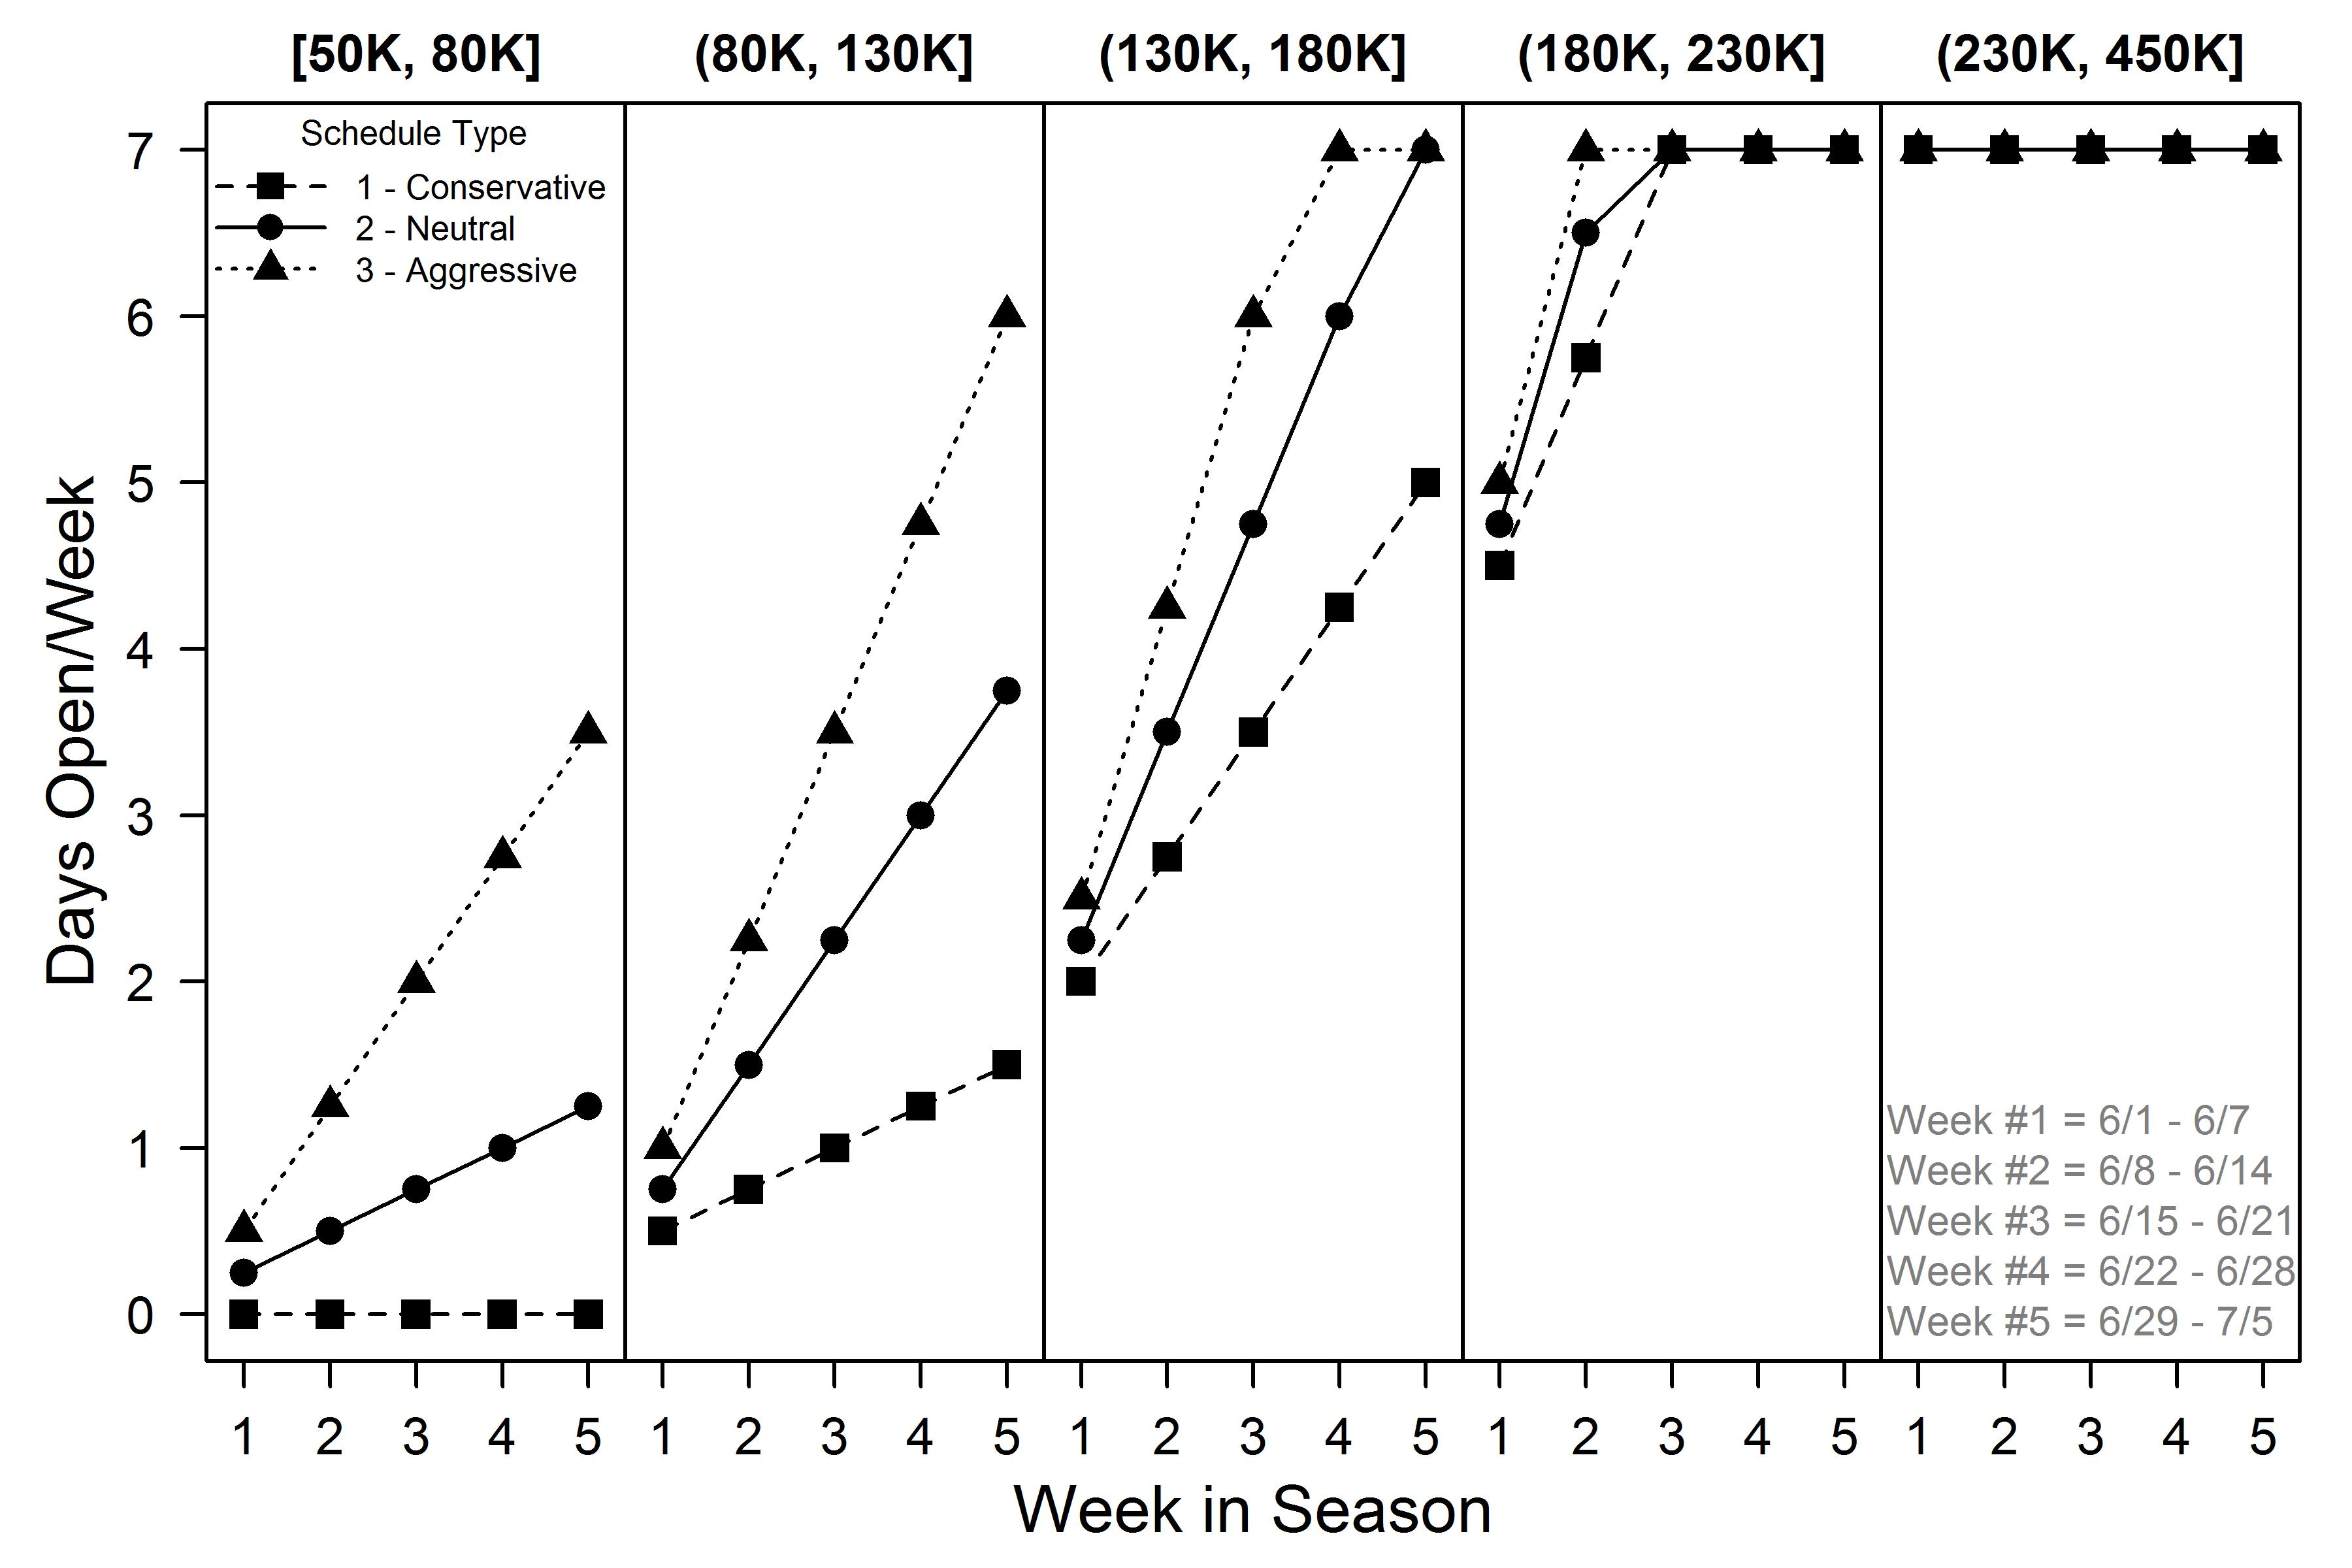
\includegraphics{img/Ch3/Schedules.png}
  \caption{Representation of the harvest control rule in assessed Strategies \#2 and \#3. The number of days the fishery is to be opened per week is a function of the pre-season forecast, as shown by each of the five panels. The three lines in each panel represent the different substrategies of Strategy \#2 or schedule types for Strategy \#3. In Strategy \#3, the manager would select to be conservative, neutral, or aggressive based on the percentile of recently-observed species ratios, as indicated in Table \ref{tab:ms3-ratio-table}. In other words, the manager using Strategy \#3 could adapt fishing schedules to in-season conditions, where as the \#2 manager could not.}
  \label{fig:ms2-schedules}
\end{figure}

\clearpage

\begin{figure}
  \centering
  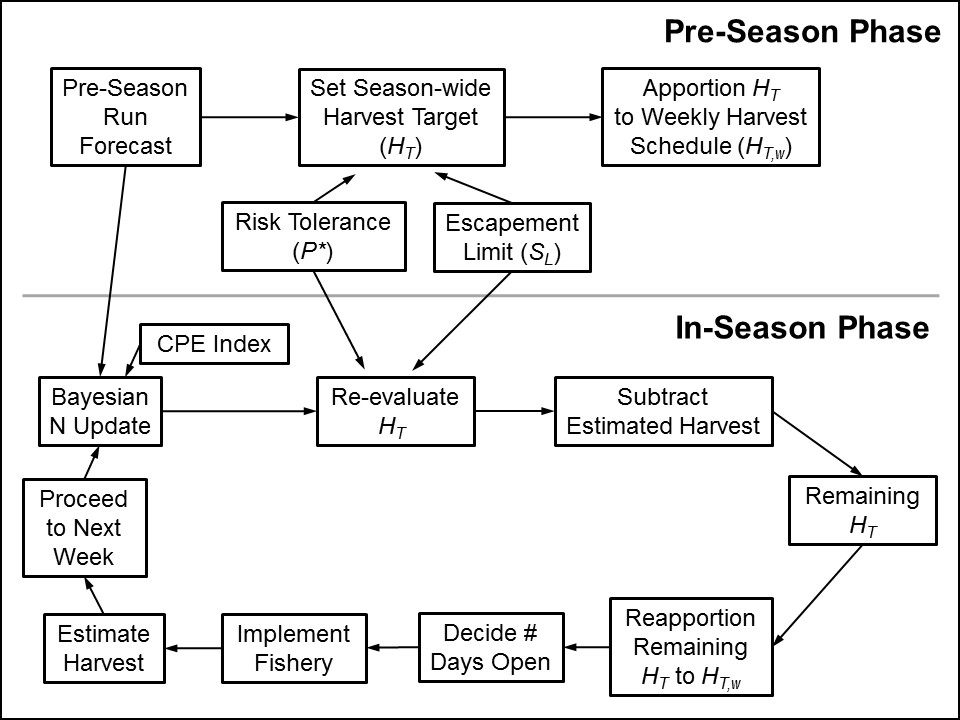
\includegraphics{img/Ch3/ms4-flow-diag.jpg}
  \caption{Depiction of the use of information to guide decision-making in assessed Strategy \#4, partitioned into pre-season and in-season phases. All actions are taken with regards to Chinook salmon. \textbf{Pre-season actions} occur only once per season, and involve producing a pre-season forecast (with error) and using it to set a season-wide harvest target ($H_T$) based on (a) the probability distribution representing uncertainty in the pre-season forecast, (b) a limit point that escapement cannot fall below ($S_L$), and (c) the maximal acceptable probability for seeing the outcome $S < S_L$ ($P^*$). Targeted harvest by week ($H_{T,w}$) is initially set by apportioning the total among weeks according to a fixed schedule based on historical run timing data. \textbf{In-season actions} are represented by a weekly cycle that involves updating perceptions of abundance and adapting the season-wide harvest target $H_T$ as appropriate to ensure the current posterior probability of attaining at least $S_L$ given $H_T$ still conforms with $P^*$, and the remaining allowable harvest for the season is obtained \textit{via} subtracting cumulative estimated harvest already taken. Remaining harvest is then apportioned to the remaining weeks, and based on the value of $H_{T,w}$, the fishery will be opened for between 0 and 7 days for the week according to the harvest tables displayed in Figure \ref{fig:ms4-schedules}. Harvest outcomes are monitored such that a weekly harvest estimate is available for use in the next week, which begins with obtaining a new posterior understanding of total run abundance.}
  \label{fig:ms4-flow-diag}
\end{figure}

\clearpage

\begin{figure}
  \centering
  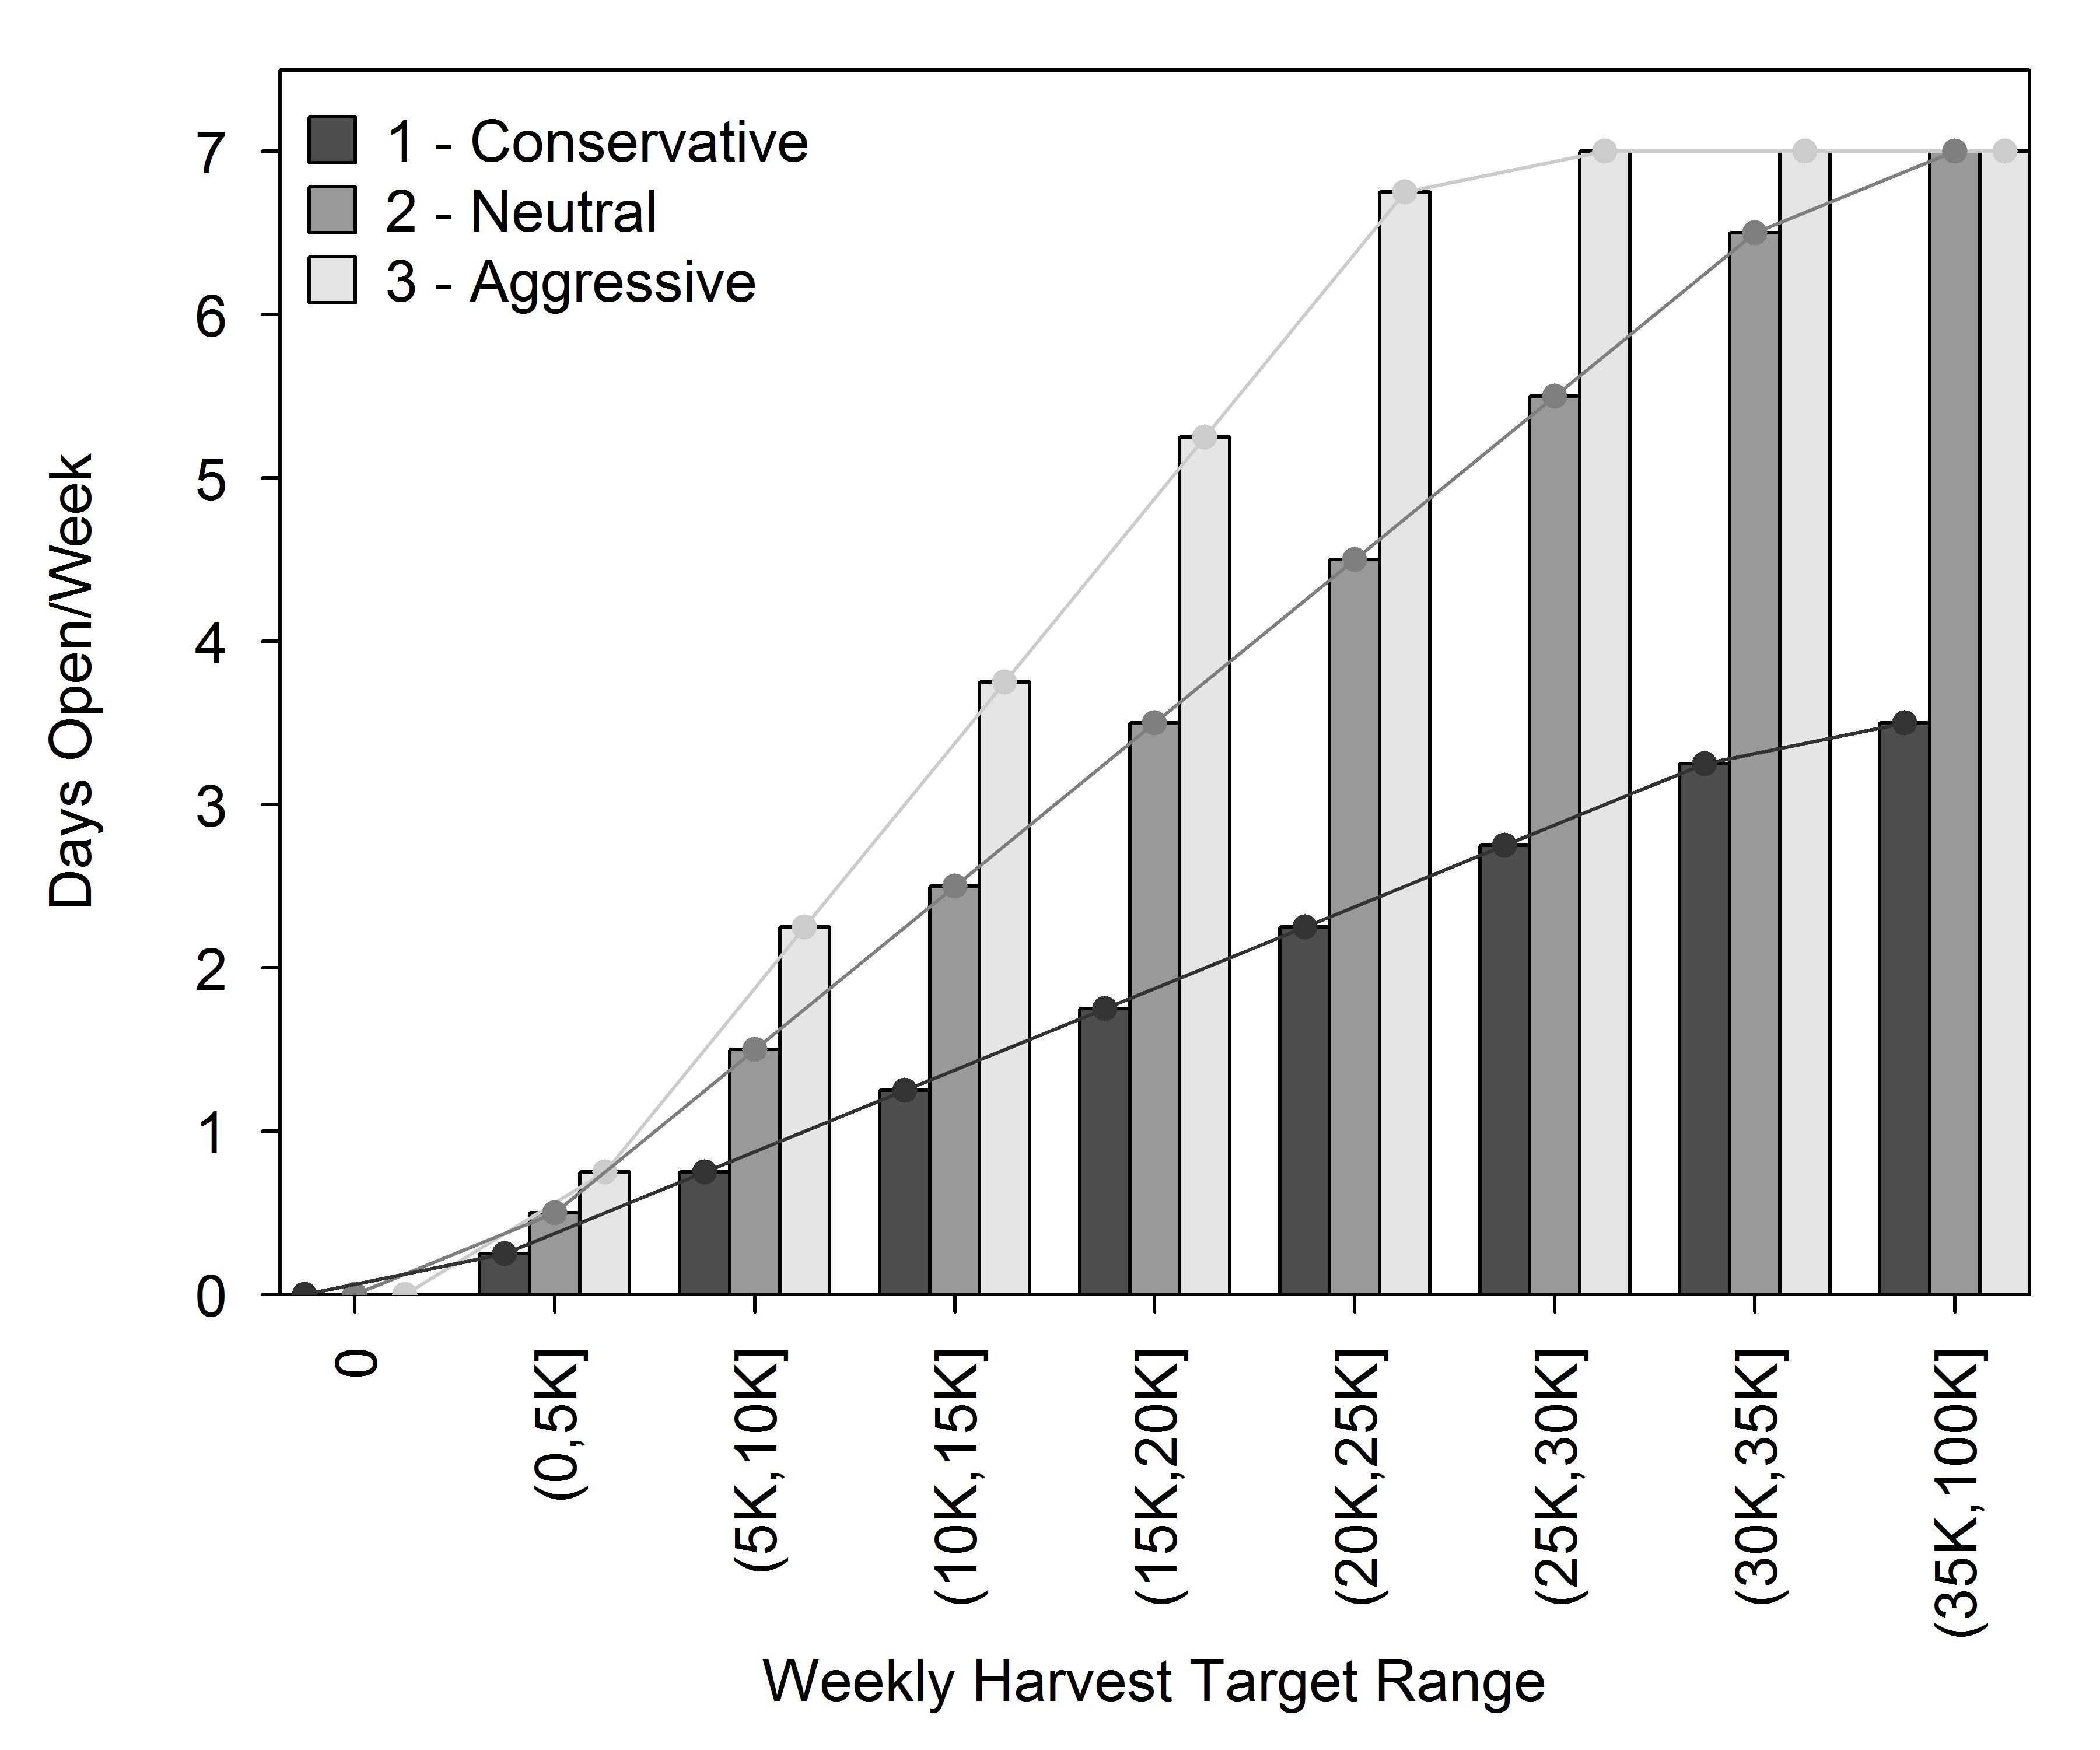
\includegraphics{img/Ch3/MS4_Schedules.jpg}
  \caption{Representation of the ``harvest tables'' used in assessed Strategy \#4. Based on how many fish are targeted each particular week ($H_{T,w}$), the manager would select the number of days to open the fishery. The process to obtain $H_{T,w}$ was rather involved, requiring pre-season forecasts, in-season abundance index data, and in-season harvest data to inform its value, as shown in Figure \ref{fig:ms4-flow-diag}.}
  \label{fig:ms4-schedules}
\end{figure}

\clearpage

\begin{figure}
  \centering
  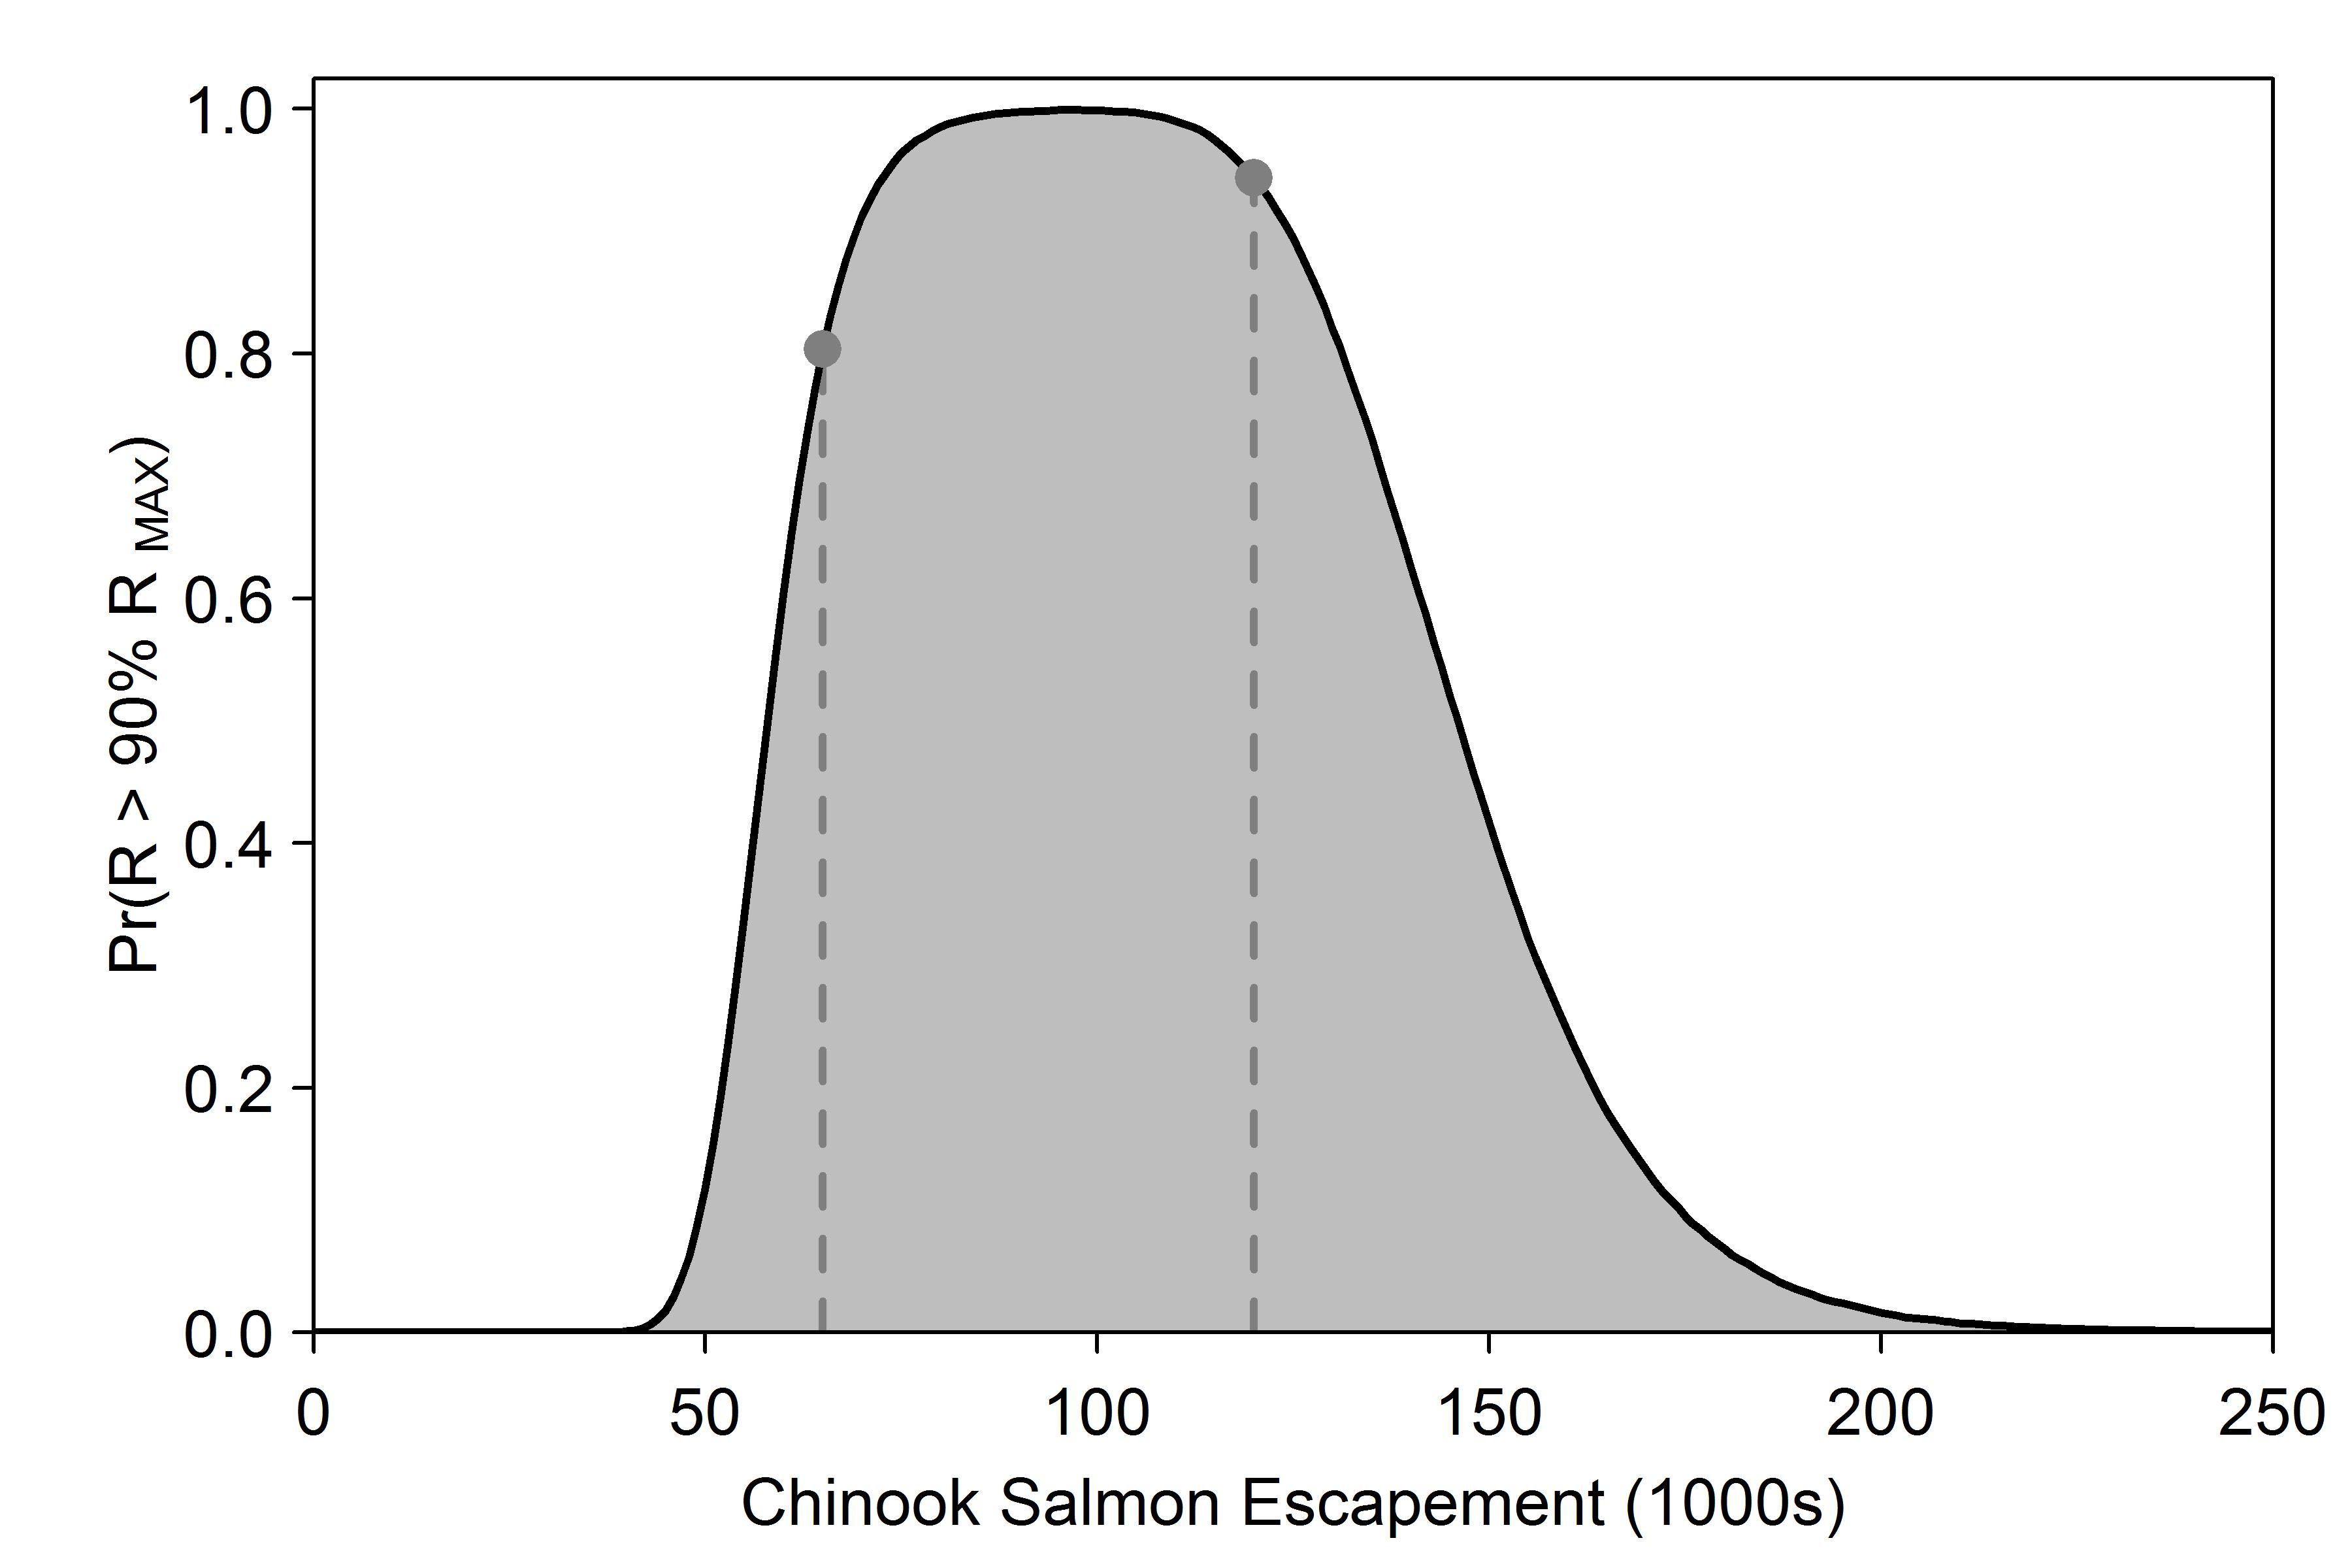
\includegraphics{img/Ch3/R-max-profile.jpg}
  \caption{Estimated probability profile for Kuskokwim River Chinook salmon used as the utility function for drainage-wide escapement in this analysis. The height of the curve represents the currently understood probability that expected recruitment produced by a given escapement level will exceed 90\% of $R_{\text{MAX}}$, and was obtained for the aggregate Chinook salmon stock using the Bayesian state-space estimation model presented in \cite{hamazaki-etal-2012} updated with abundance, harvest, and age composition data through 2017. The vertical dashed lines are the endpoints of the current escapement goal range: 65,000 -- 120,000.}
  \label{fig:R-max-profile}
\end{figure}

\clearpage
\begin{figure}
  \centering
  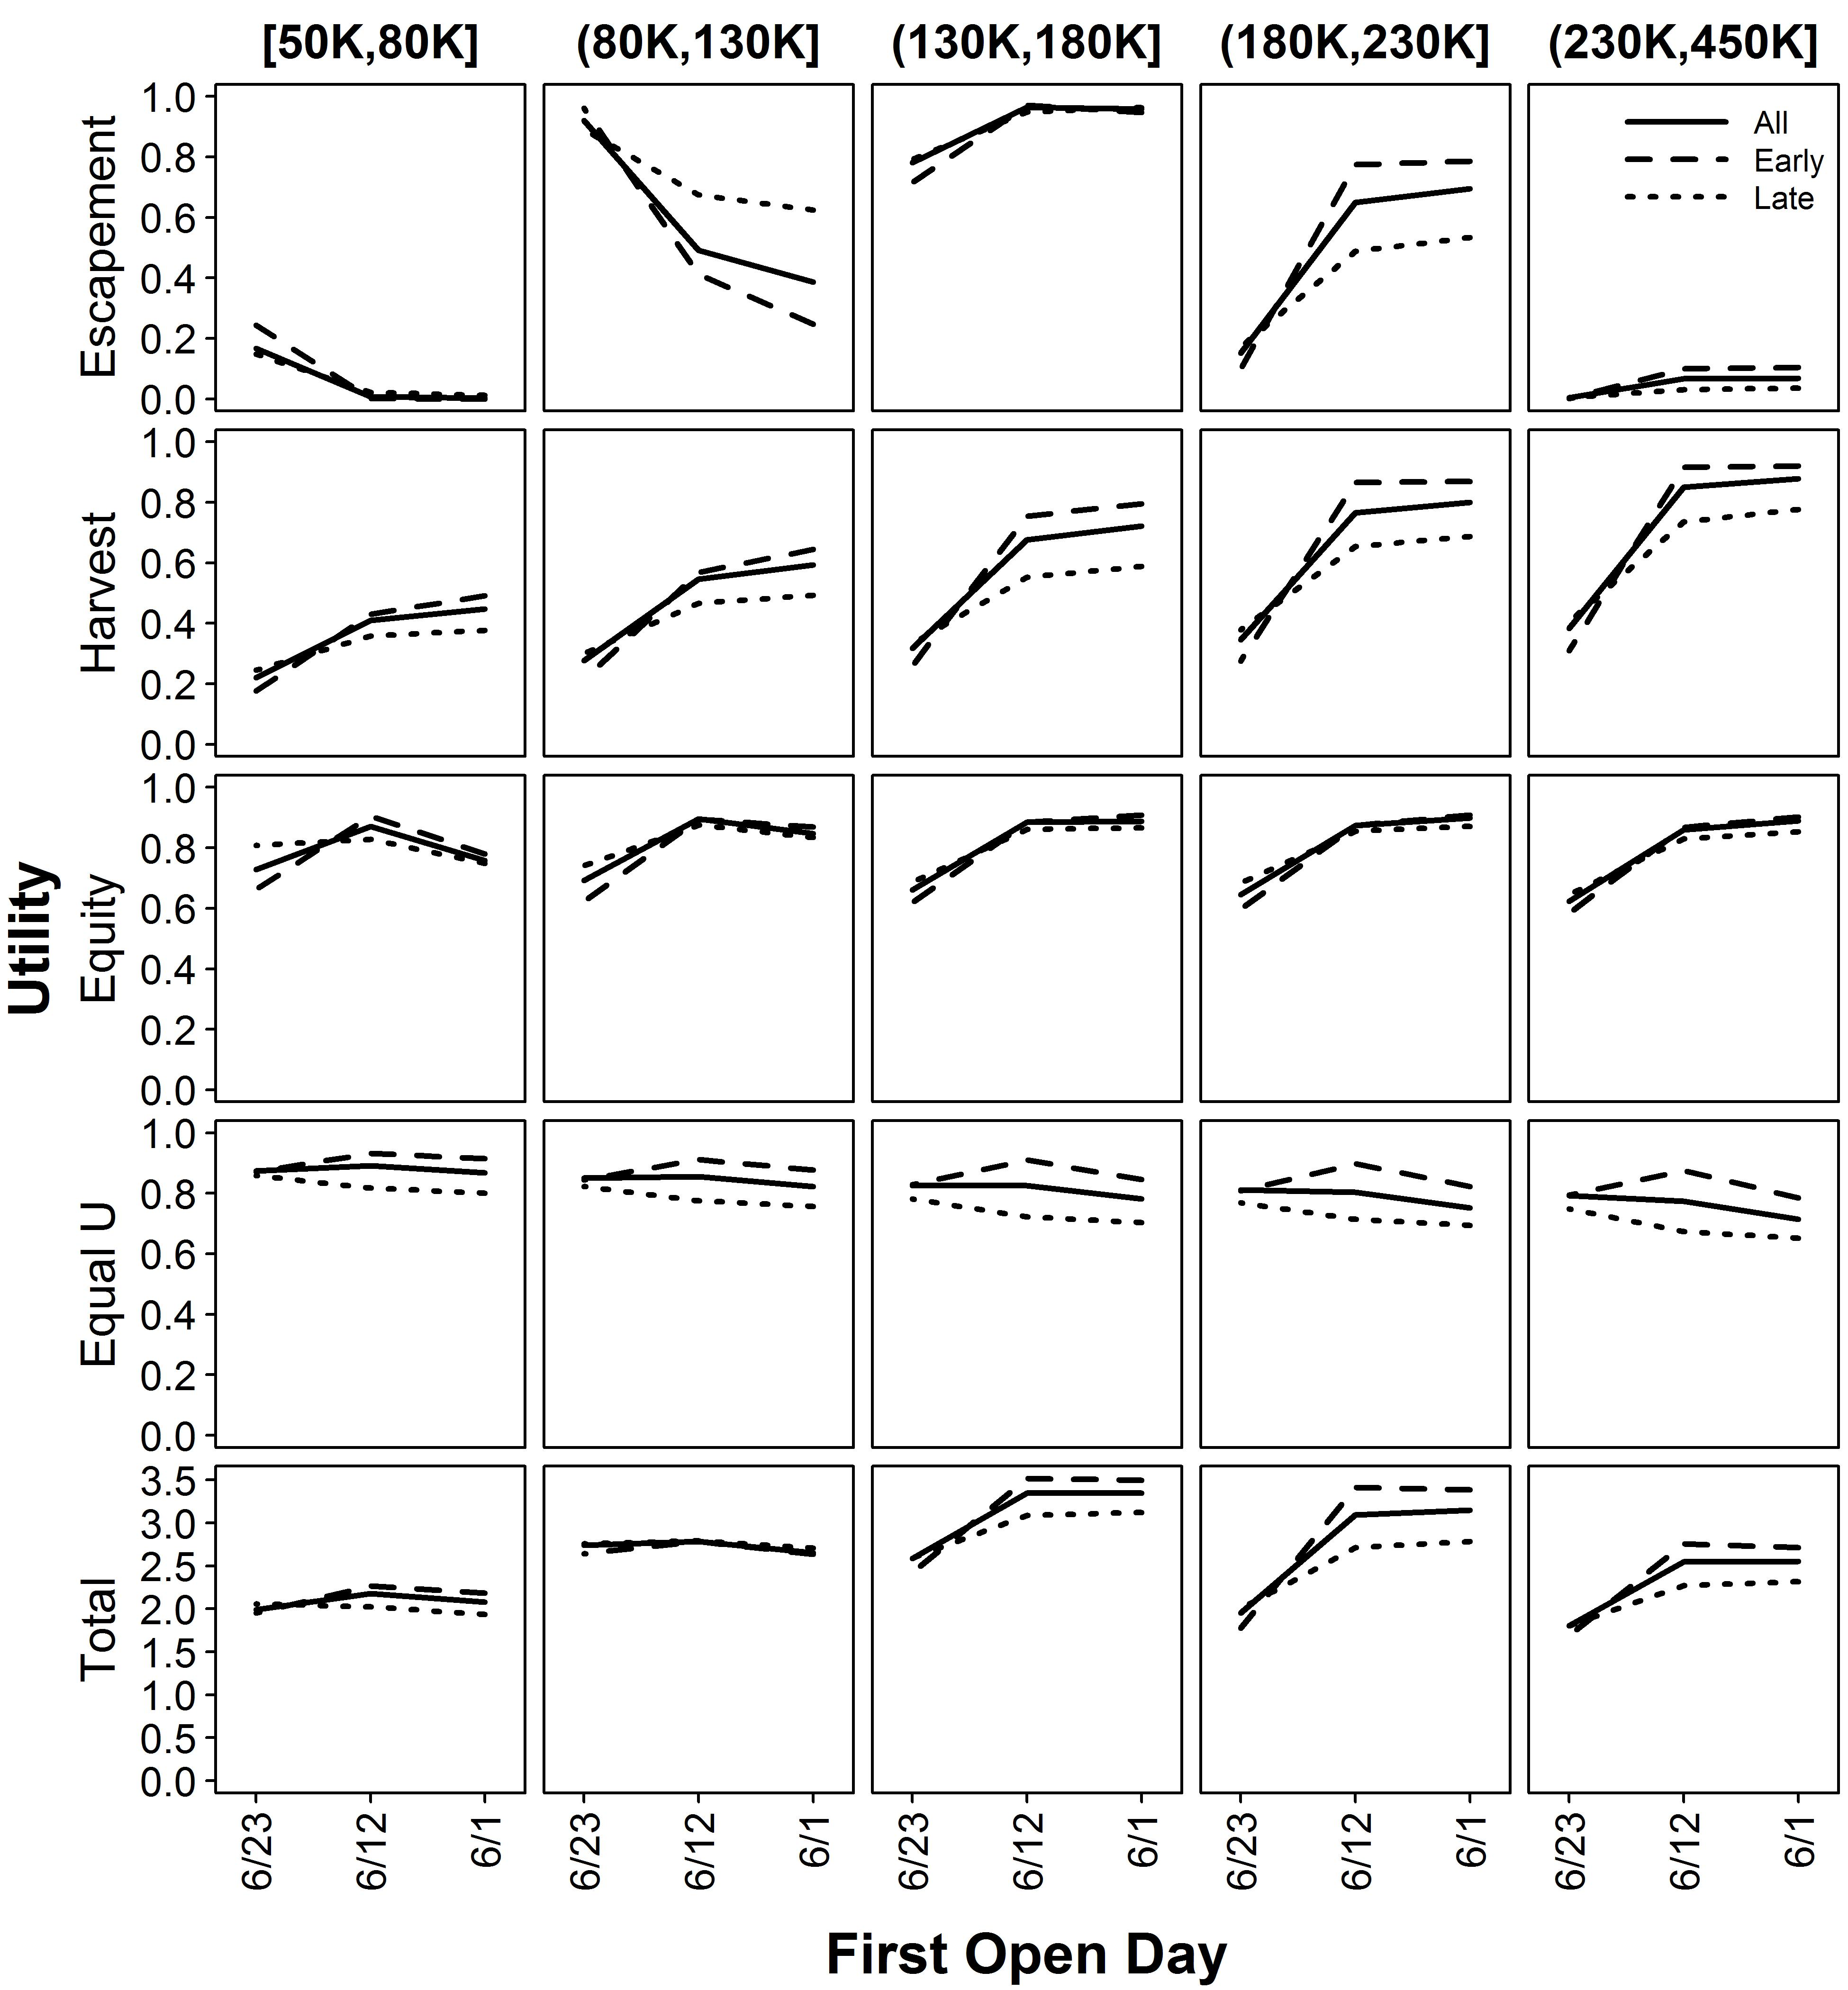
\includegraphics{img/Ch3/Values_1.jpg}
  \caption{Detailed performance of assessed Strategy \#1. Values of the utility functions (rows) separated by run size category (horizontal panels), run timing category (line type), and substrategy ($x$-axis, ordered from most conservative to aggressive). Substrategies of this policy differ in the date at which the fishery is opened completely. The form of each utility function is described in Section \ref{utility-funcs}, and the total metric shown uses the default weighting scheme (all objective weights equal to 1).}
  \label{fig:ms1-utilities}
\end{figure}

\clearpage
\begin{figure}
  \centering
  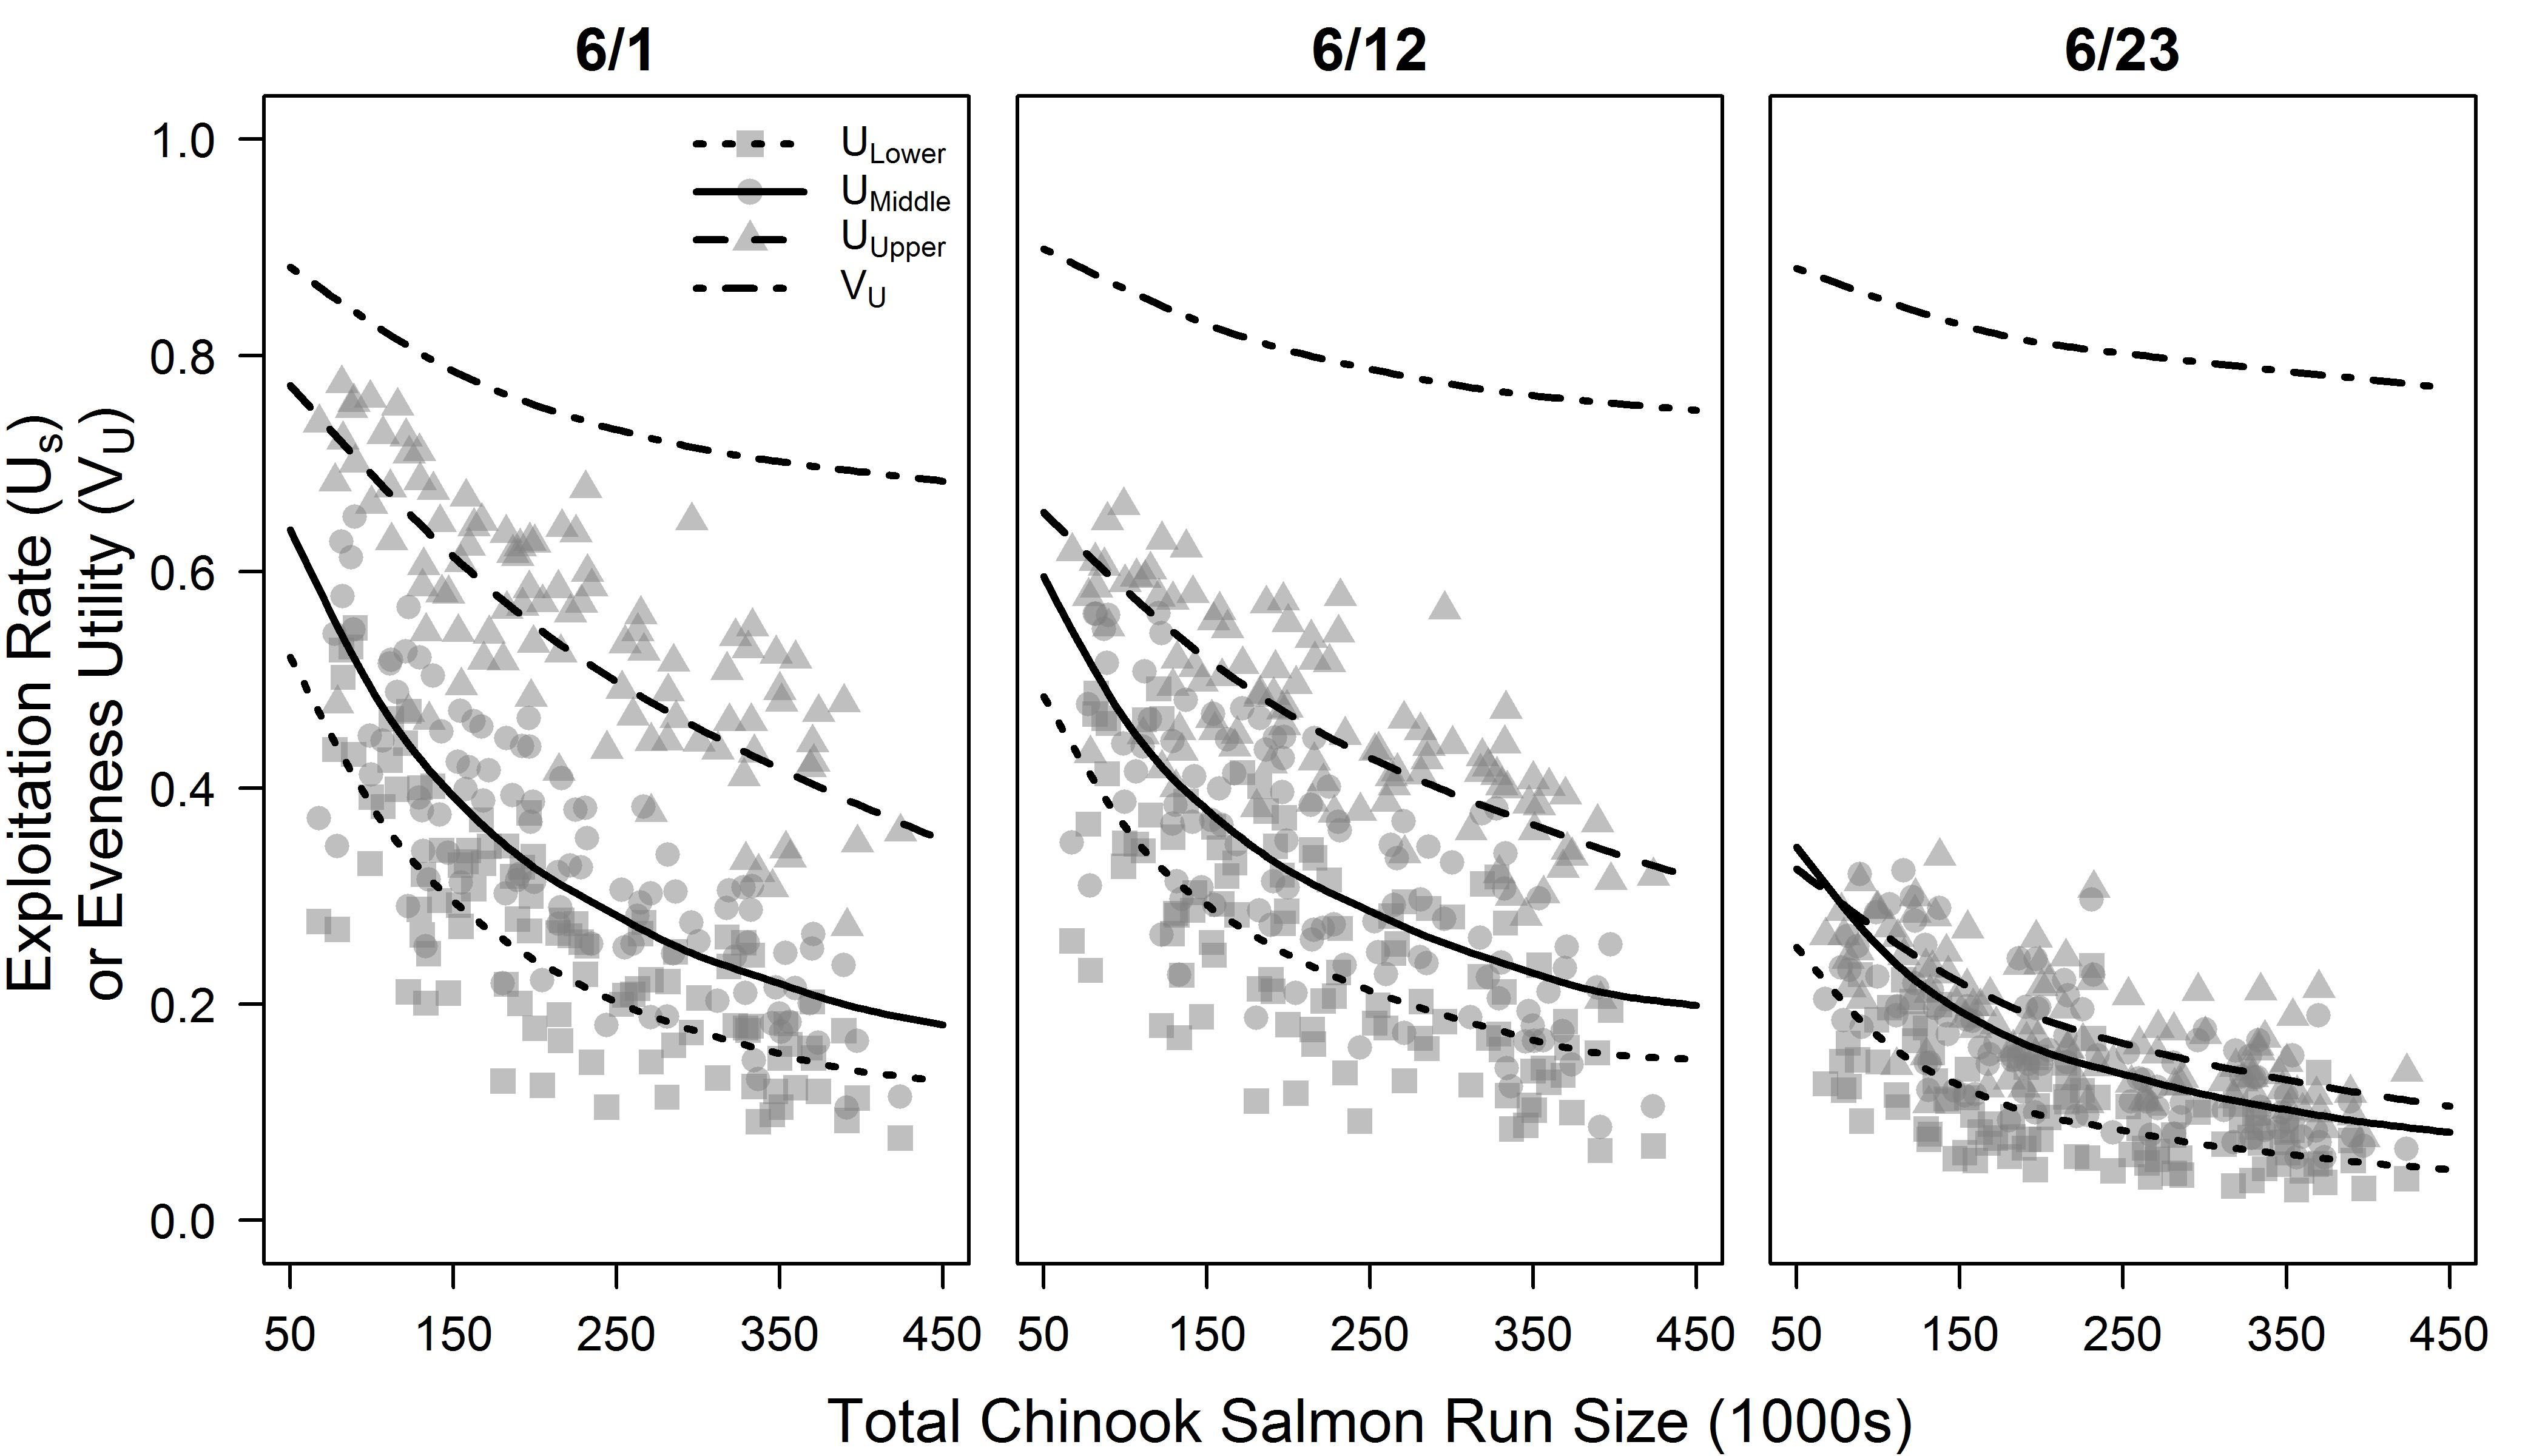
\includegraphics{img/Ch3/U-v-N.jpg}
  \caption{Chinook salmon substock-specific exploitation rates as a function of run size from 500 Monte Carlo trials, separated by different substrategies (i.e., opening dates) of assessed Strategy \#1. Lines are fitted generalized additive models. The line denoted by $V_U$ represents the model fitted to the utility metric as defined by the modified Schutz coefficient used (points not shown).}
  \label{fig:U-v-N}
\end{figure}

\clearpage
\begin{figure}
  \centering
  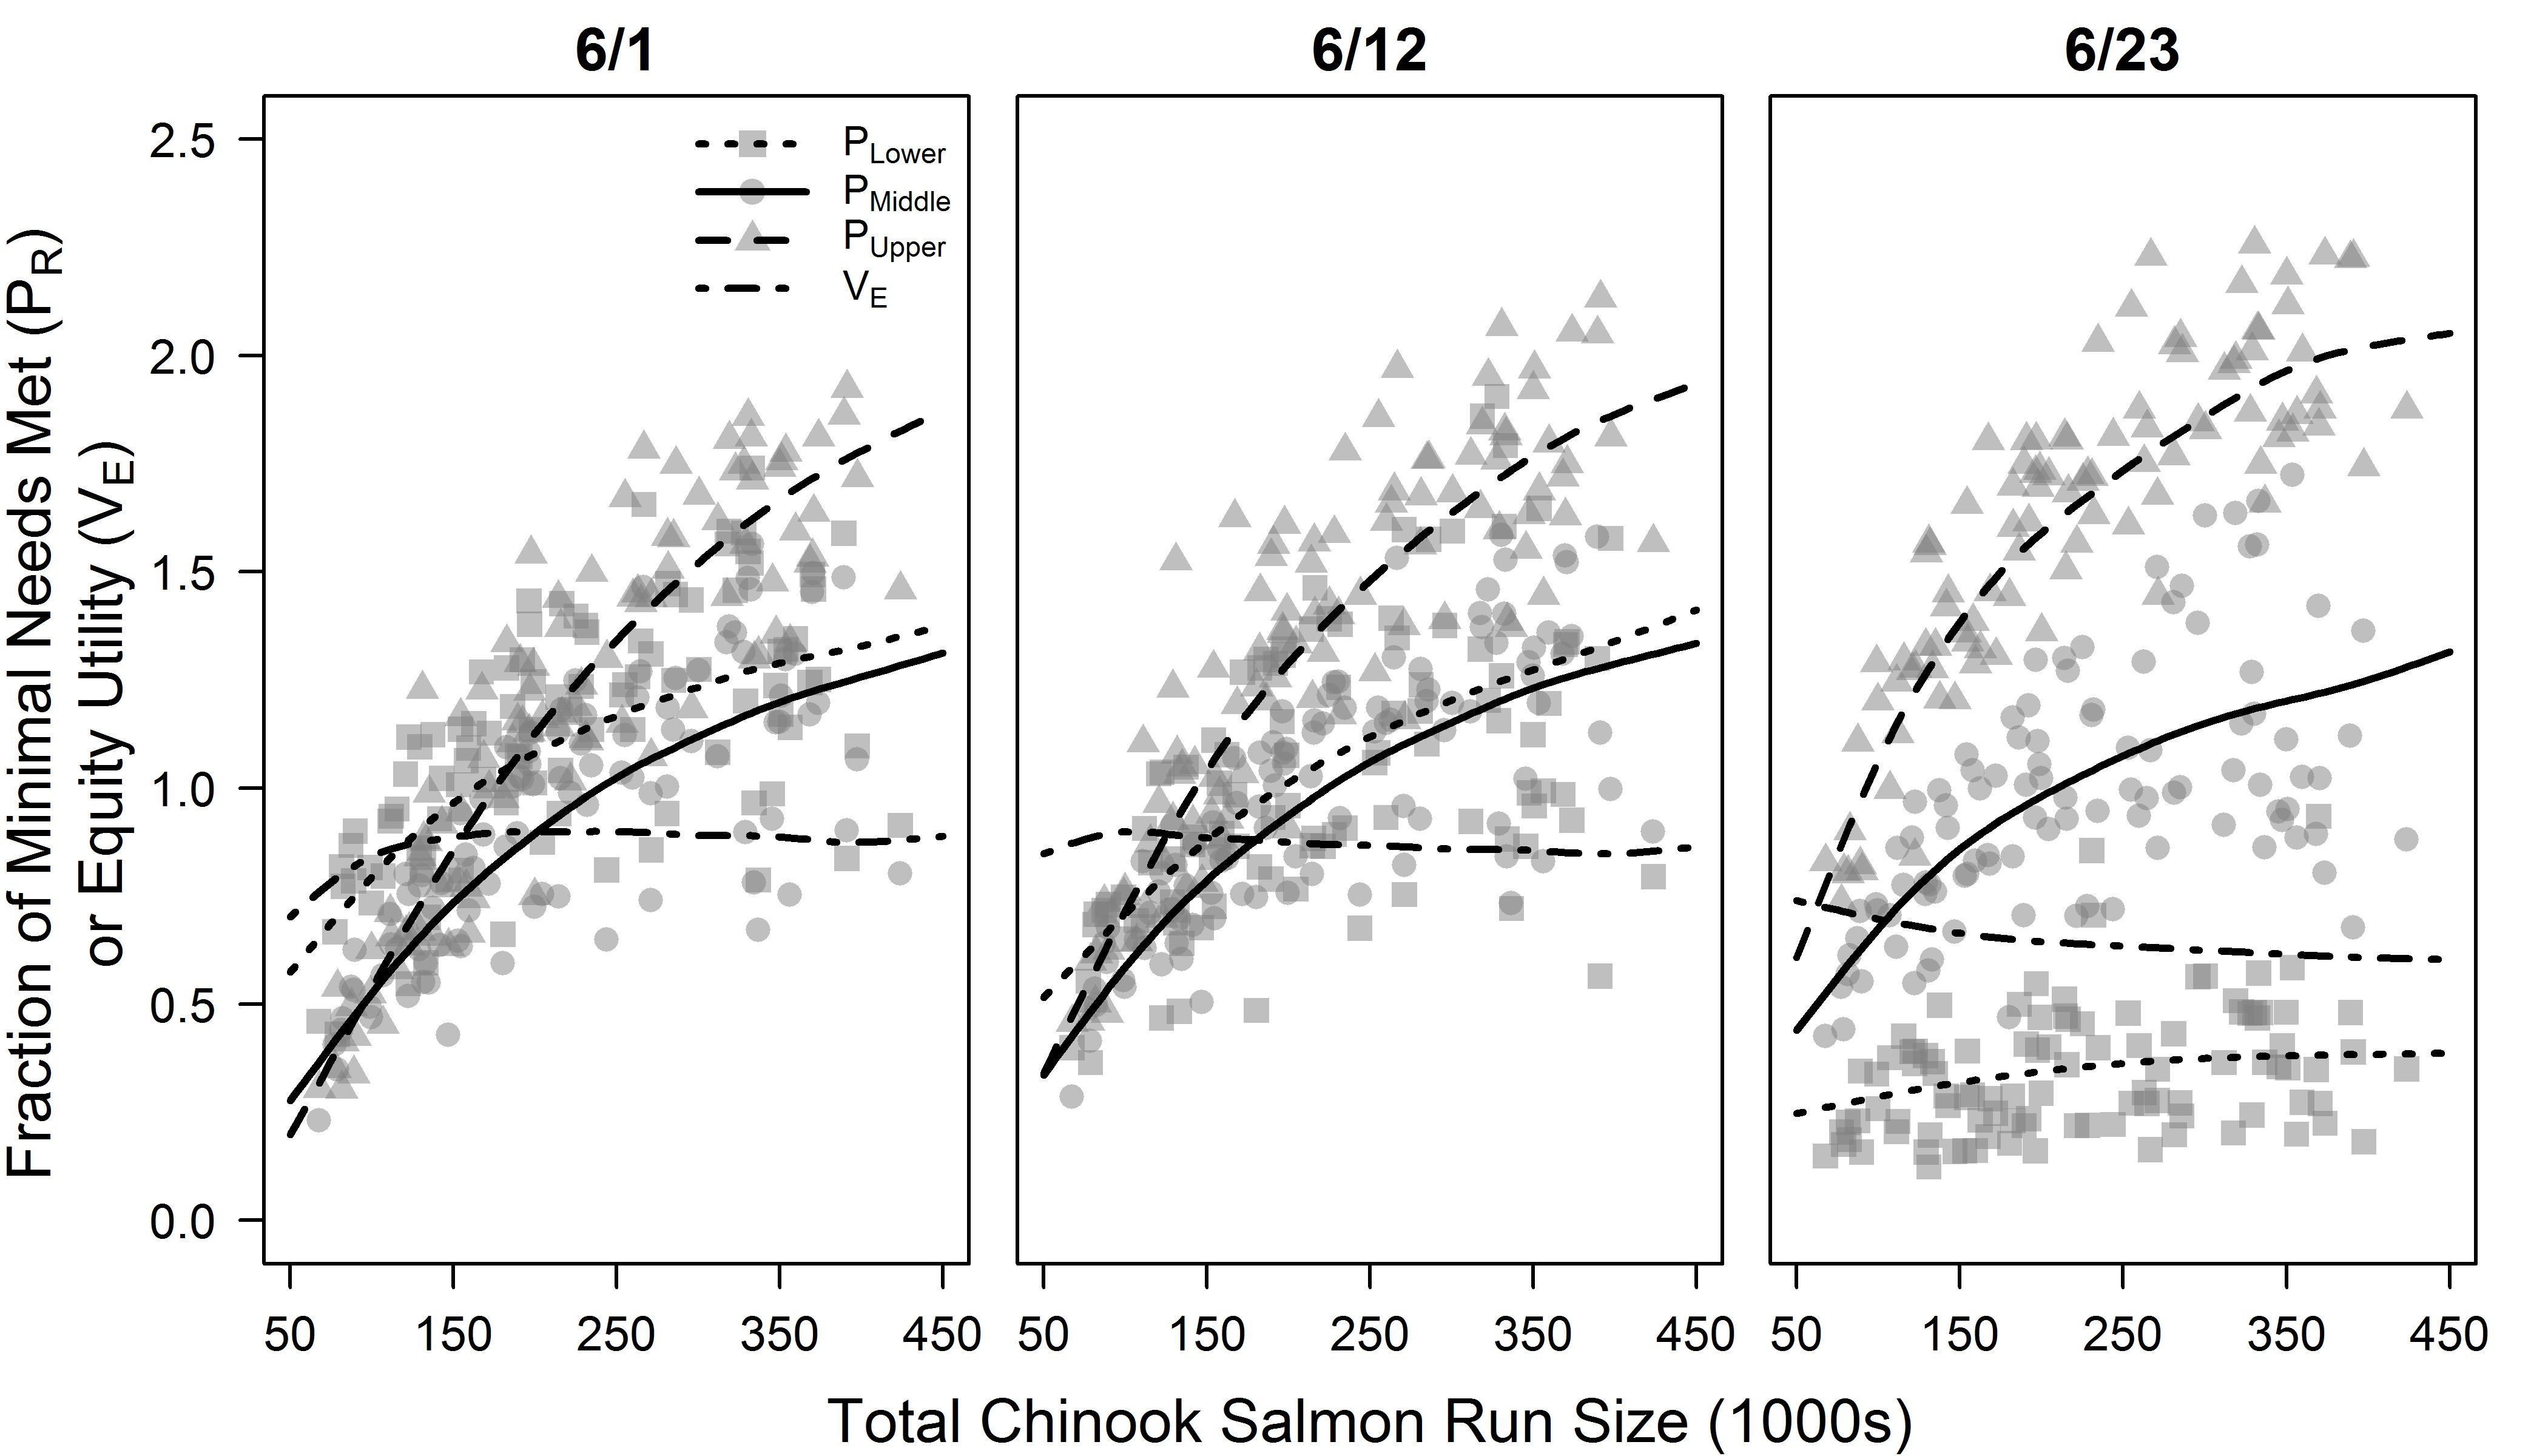
\includegraphics{img/Ch3/pNeed-v-N.jpg}
  \caption{The fraction of minimal Chinook salmon harvest attained by villages in the lower, middle, and upper regions of the simulated Kuskokwim River as a function of run size from 500 Monte Carlo trials, separated by different substrategies (i.e., opening dates) of assessed Strategy \#1. Lines are fitted generalized additive models. The line denoted by $V_E$ represents the model fitted to the utility metric as defined by the modified Schutz coefficient used (points not shown).}
  \label{fig:pNeed-v-N}
\end{figure}

\clearpage
\begin{figure}
  \centering
  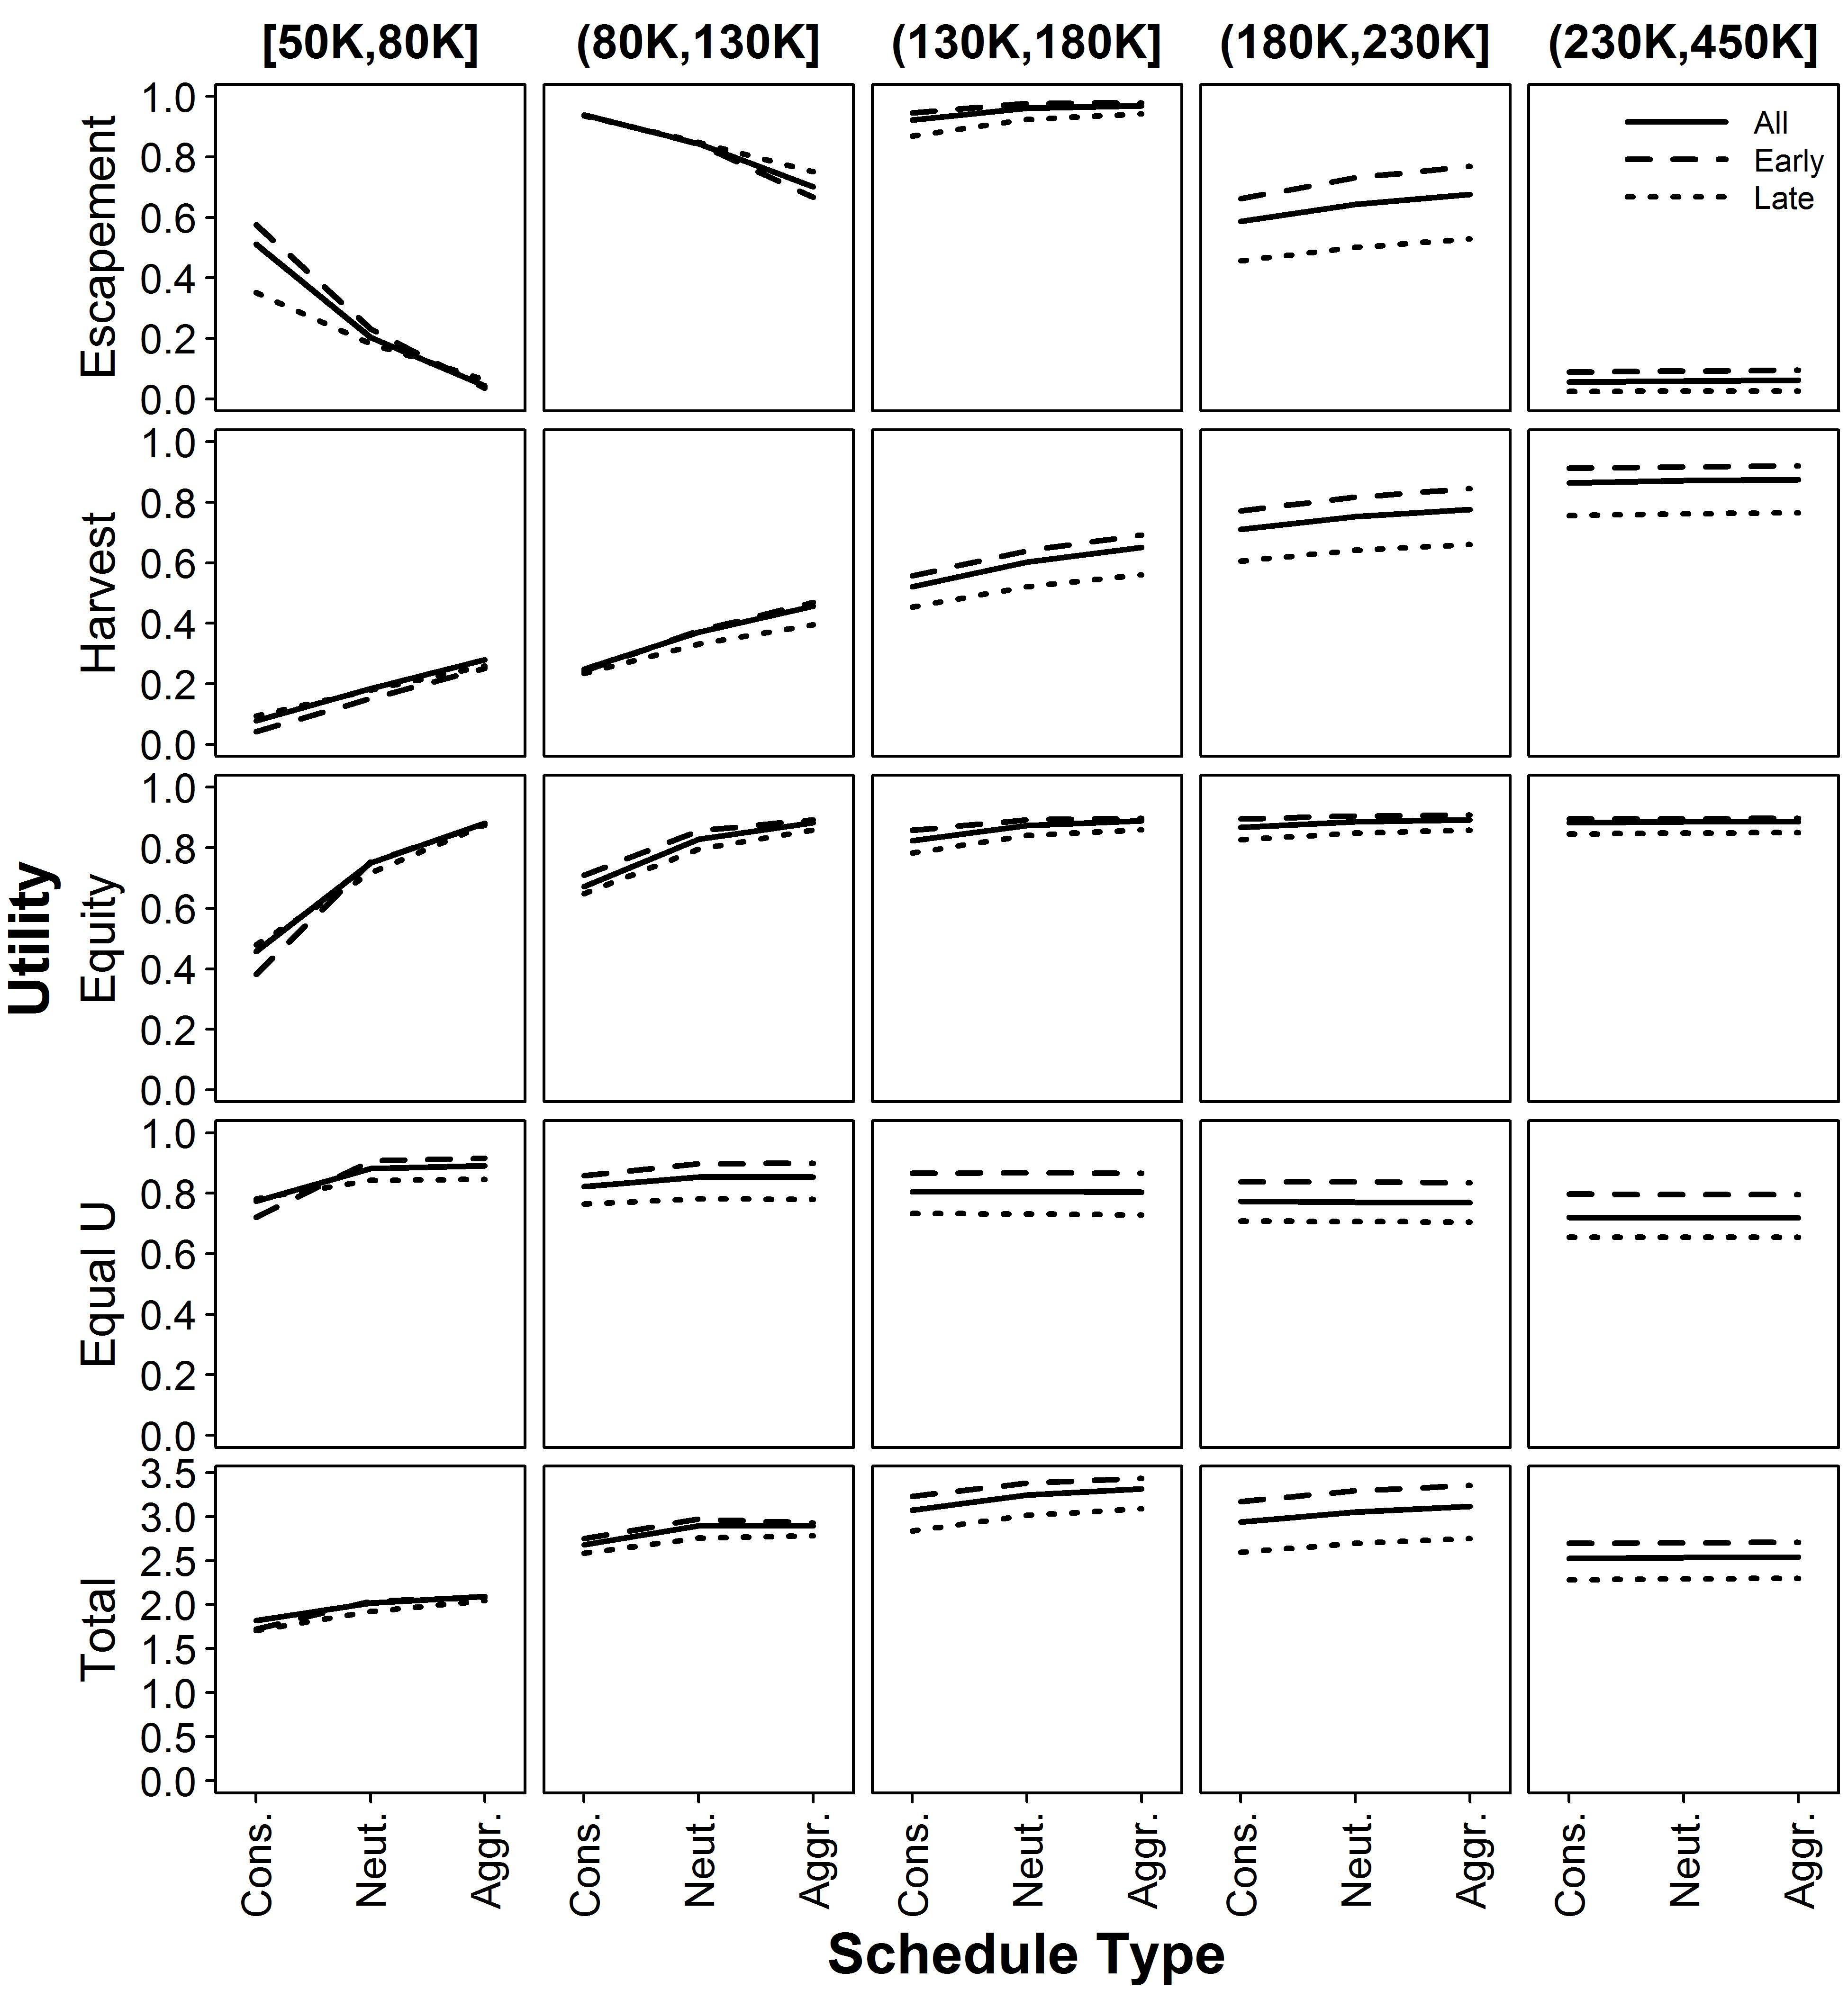
\includegraphics{img/Ch3/Values_2.jpg}
  \caption{Detailed performance of assessed Strategy \#2. The layout of panels in this figure is the same as in Figure \ref{fig:ms1-utilities}, only substrategies represent different schedules conditional on a pre-season run size forecast (schedules shown in Figure \ref{fig:ms2-schedules}).}
  \label{fig:ms2-utilities}
\end{figure}

\clearpage
\begin{figure}
  \centering
  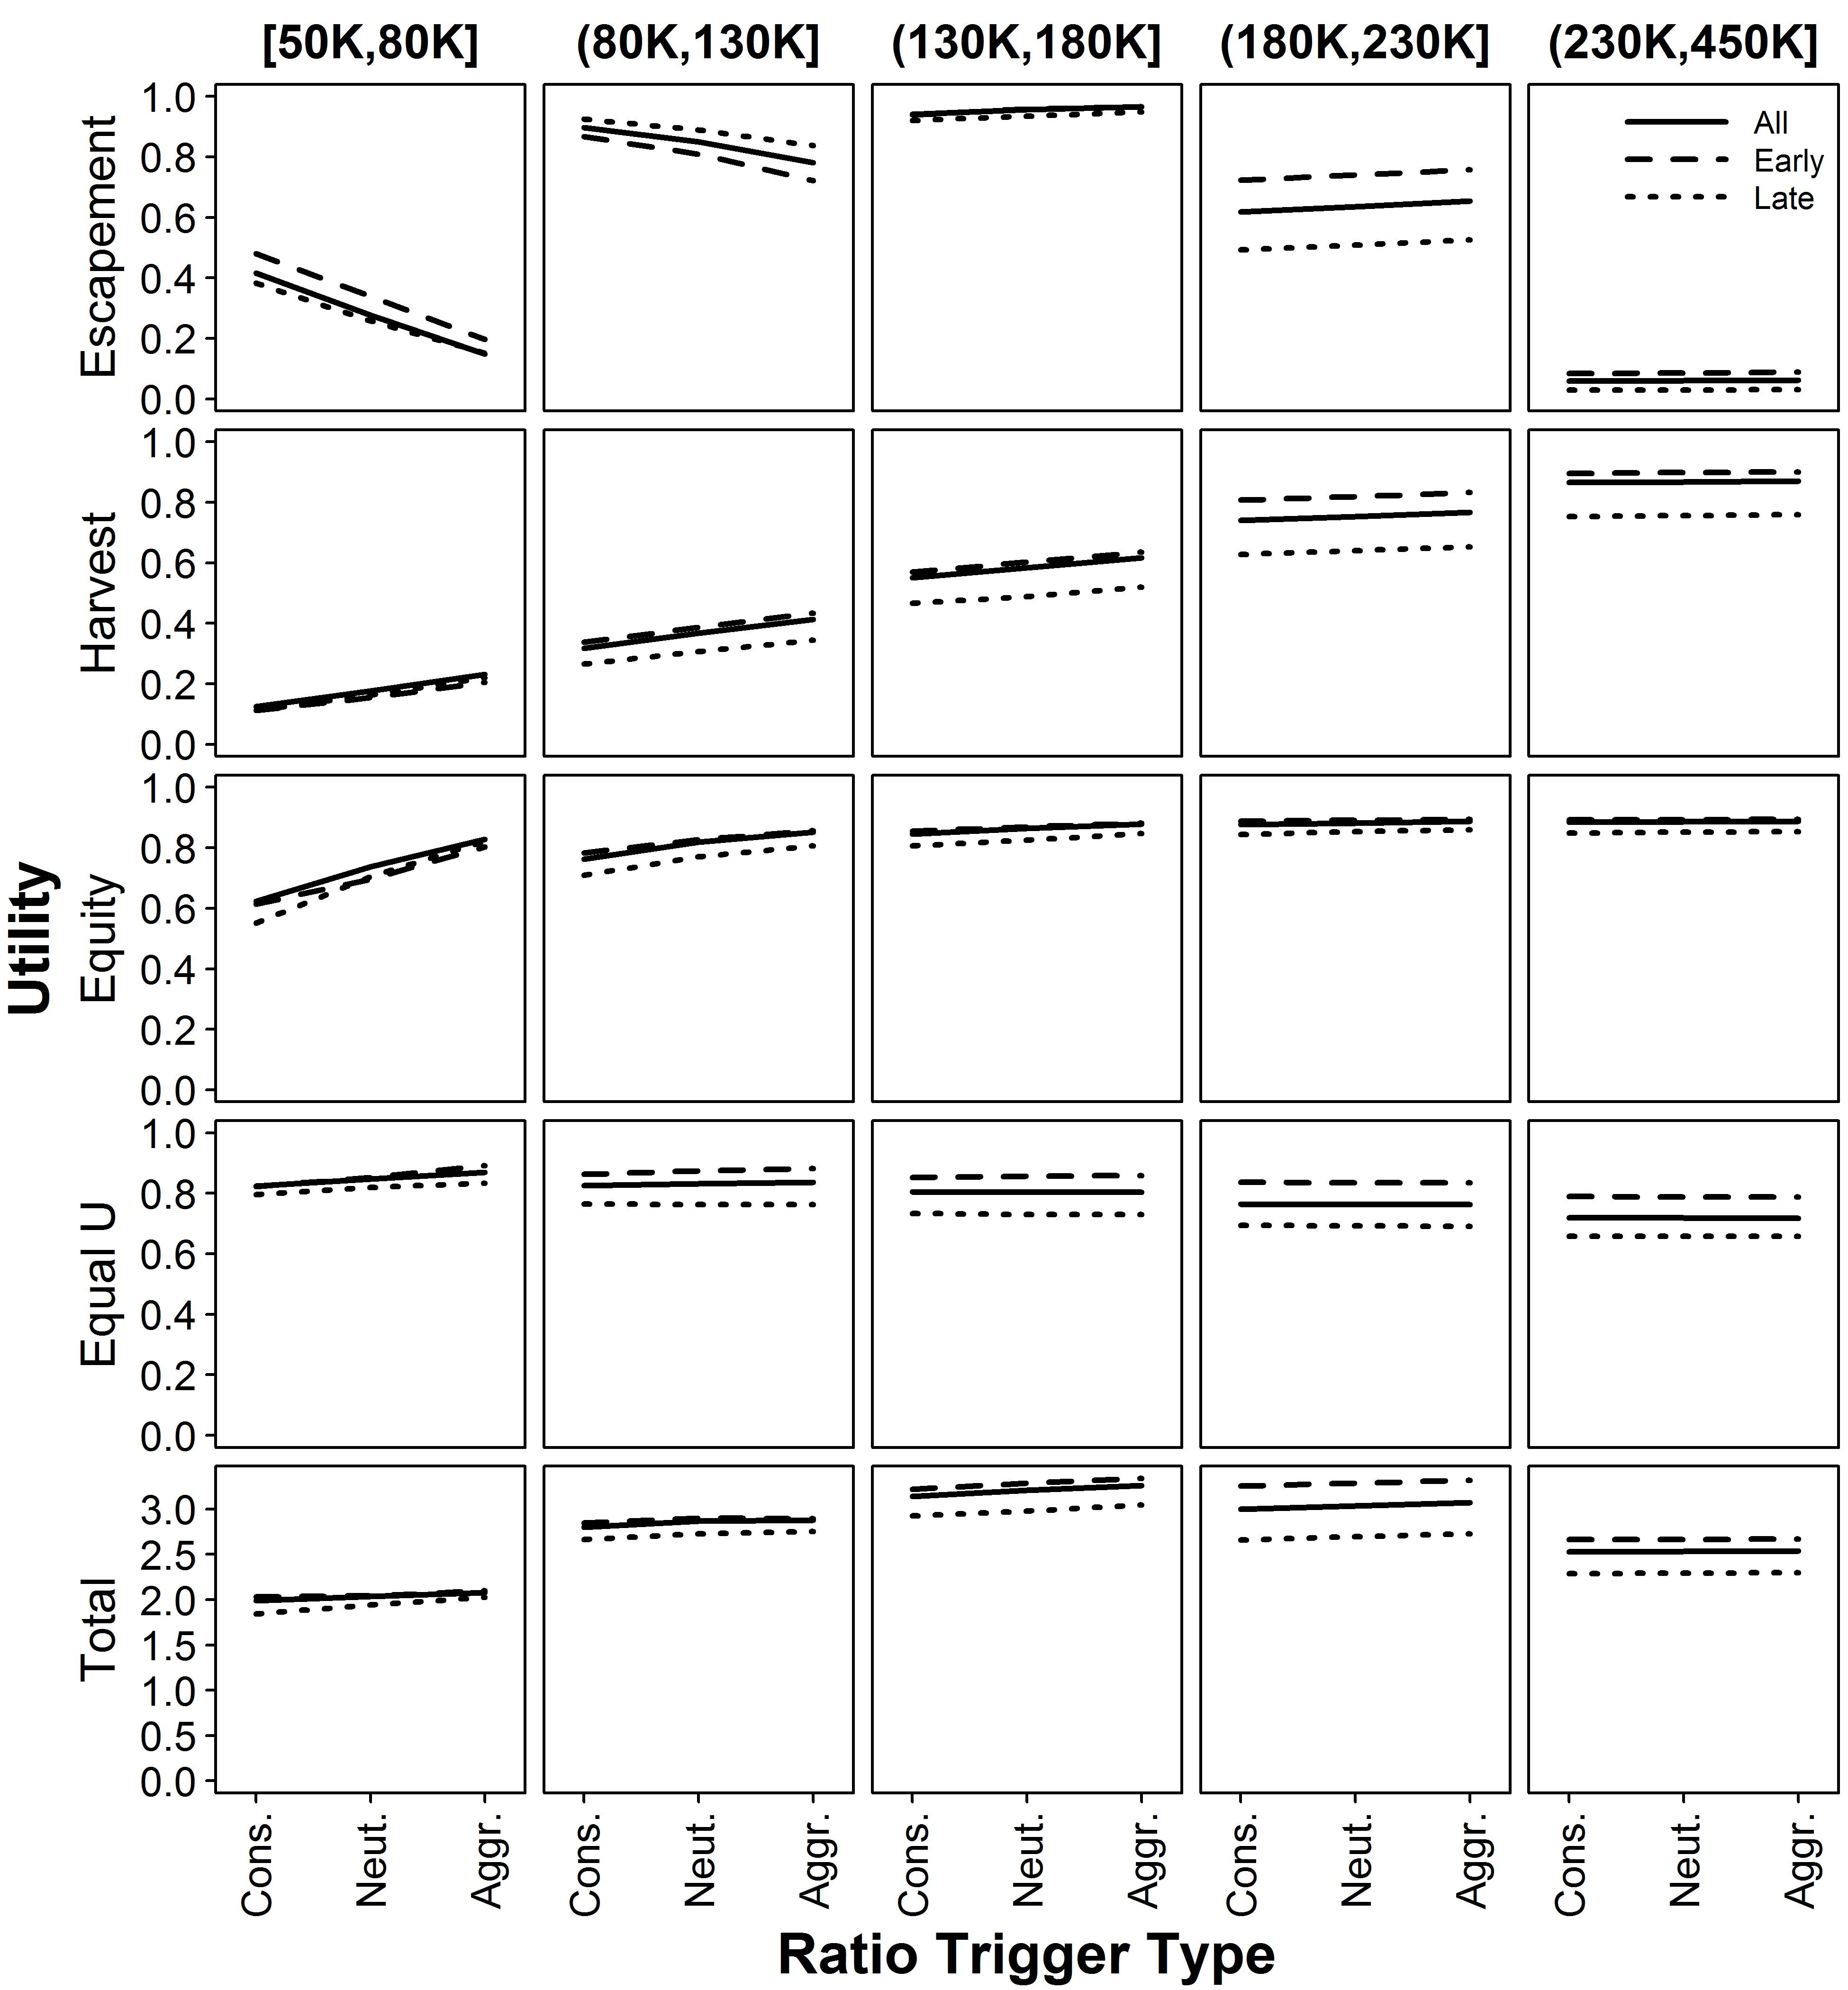
\includegraphics{img/Ch3/Values_3.jpg}
  \caption{Detailed performance of assessed Strategy \#3. The layout of panels in this figure is the same as in Figure \ref{fig:ms1-utilities}, only substrategies represent different species ratios cut-offs used to pick fishing schedules conditional on a pre-season run size forecast (schedules shown in Figure \ref{fig:ms2-schedules}, ratio thresholds shown in Table \ref{tab:ms3-ratio2-table}).}
  \label{fig:ms3-utilities}
\end{figure}

\clearpage
\begin{figure}
  \centering
  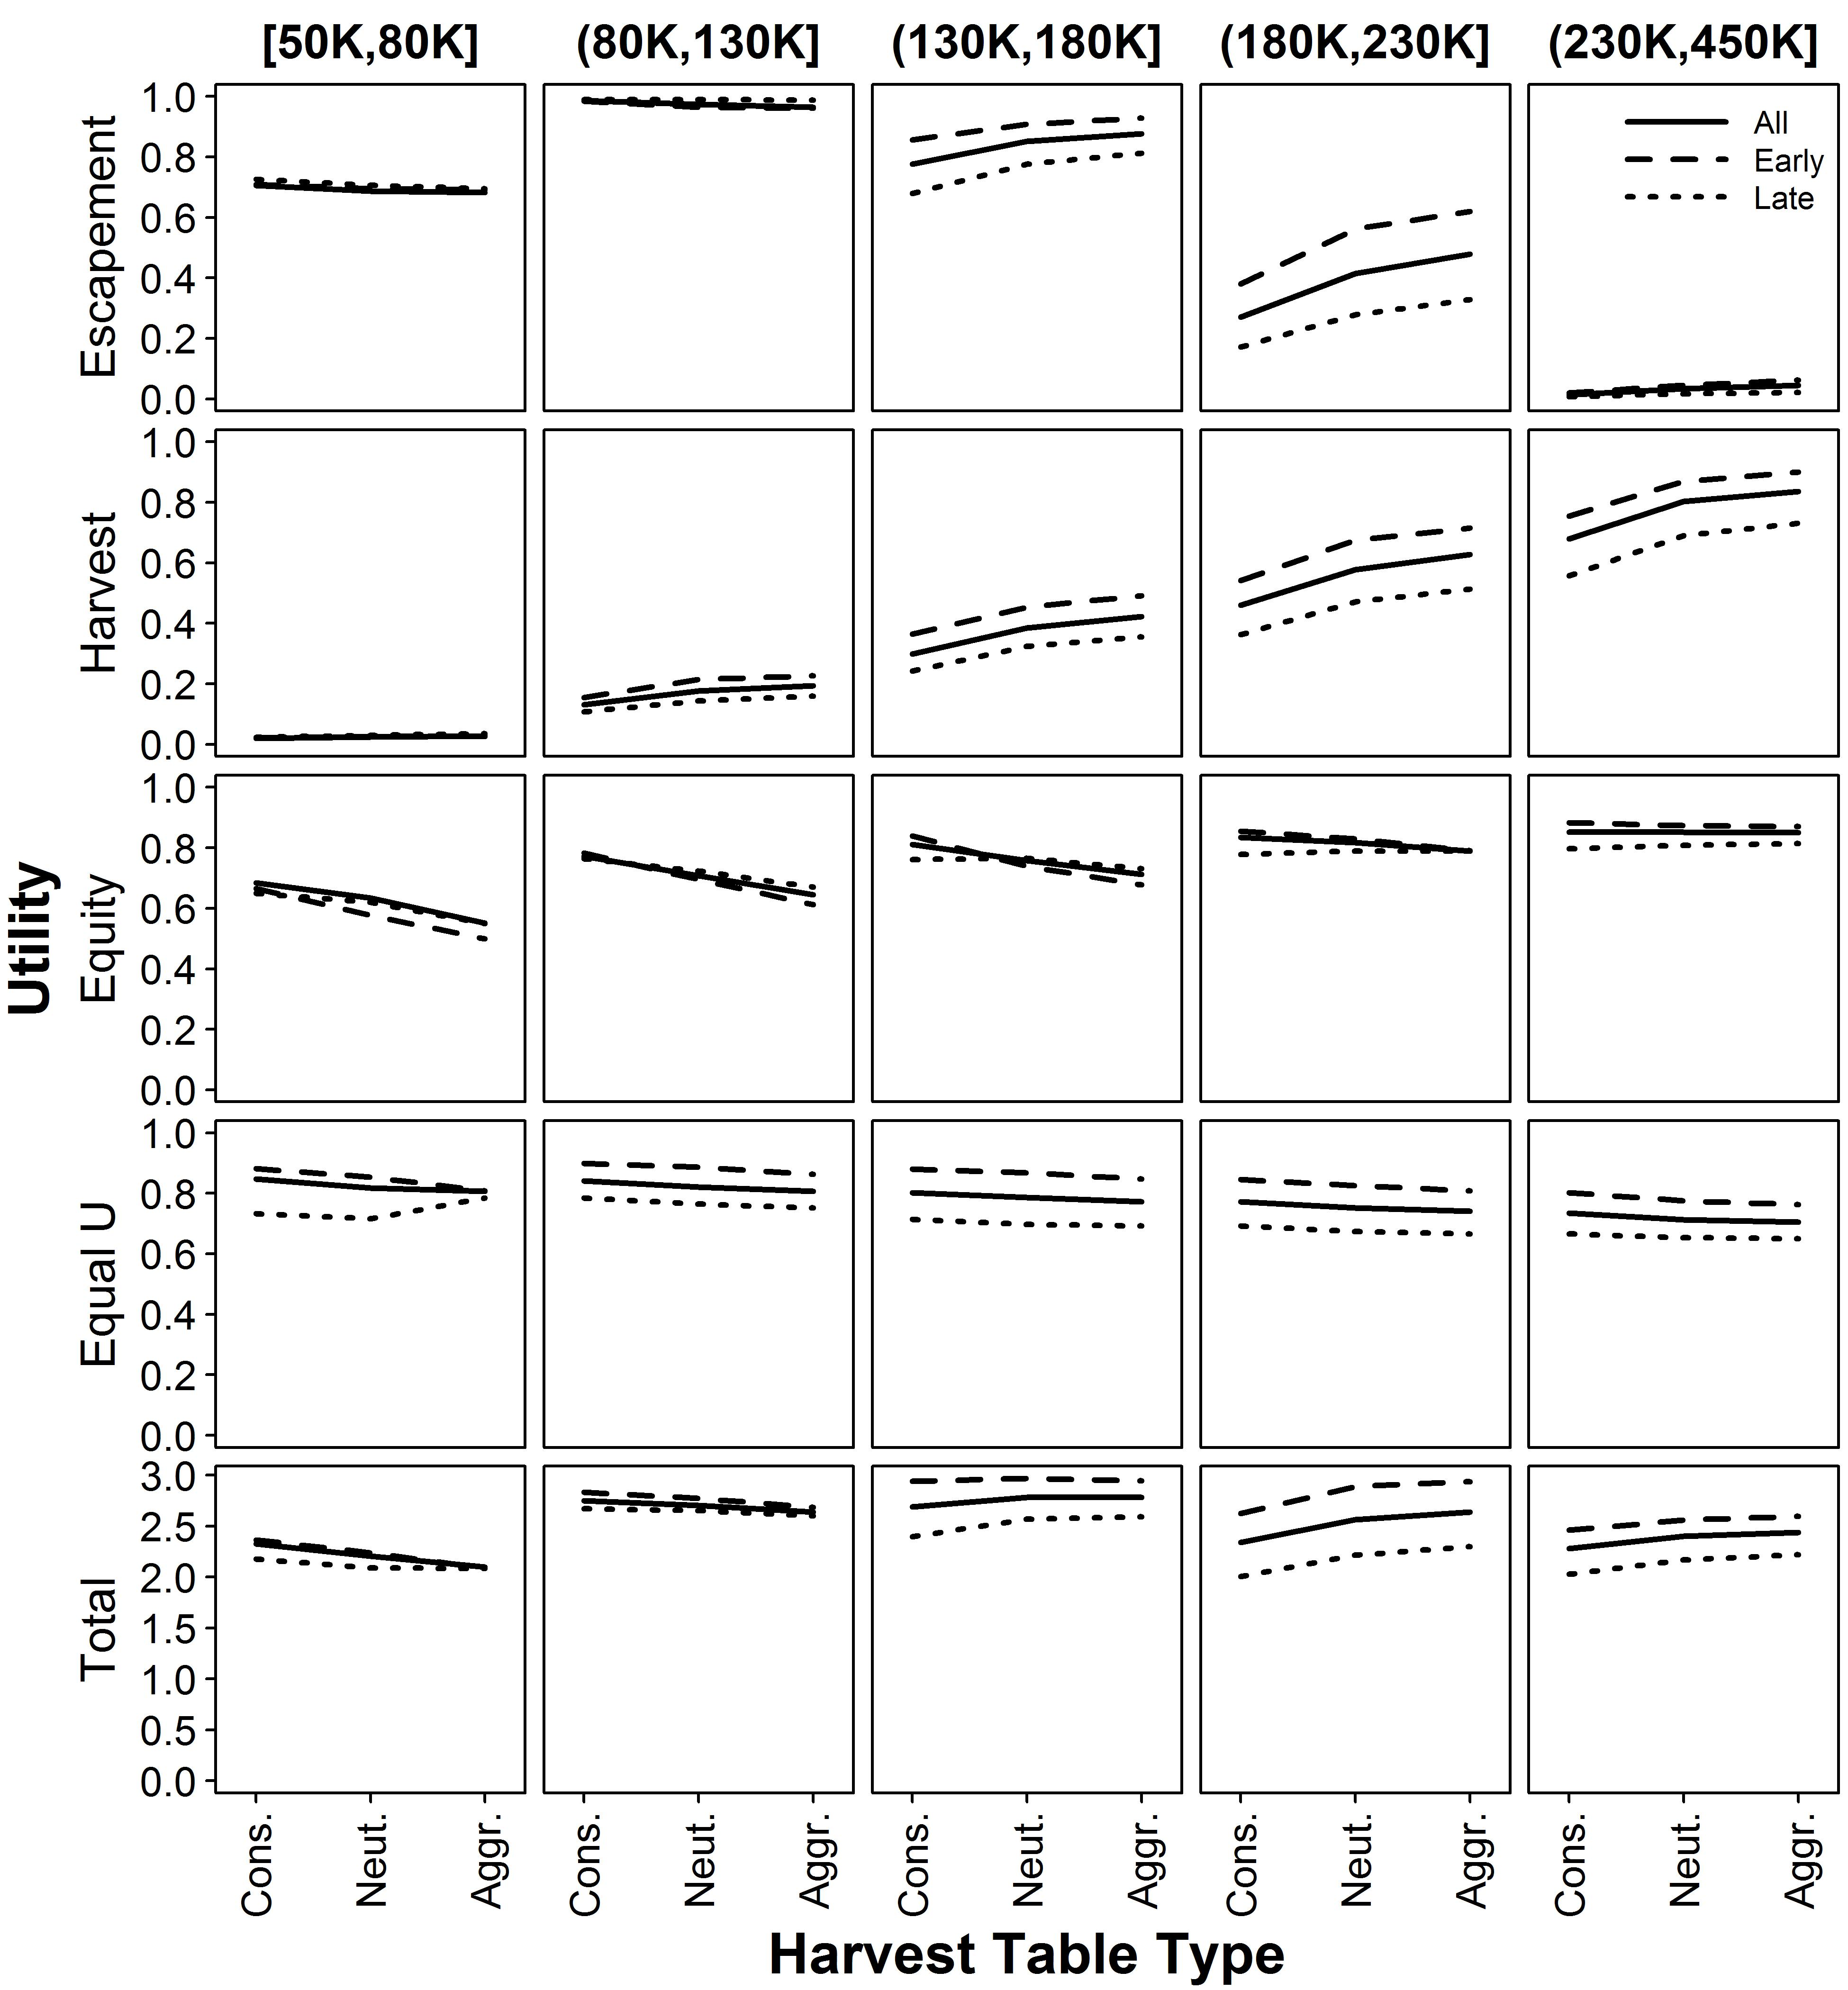
\includegraphics{img/Ch3/Values_4.jpg}
  \caption{Detailed performance of assessed Strategy \#4. The layout of panels in this figure is the same as in Figure \ref{fig:ms1-utilities}, only substrategies represent different harvest tables used to set the number of days of open fishing per week based on how many fish are targeted to be harvested that week (harvest tables shown in Figure \ref{fig:ms4-schedules}).}
  \label{fig:ms4-utilities}
\end{figure}

\clearpage
\begin{figure}
  \centering
  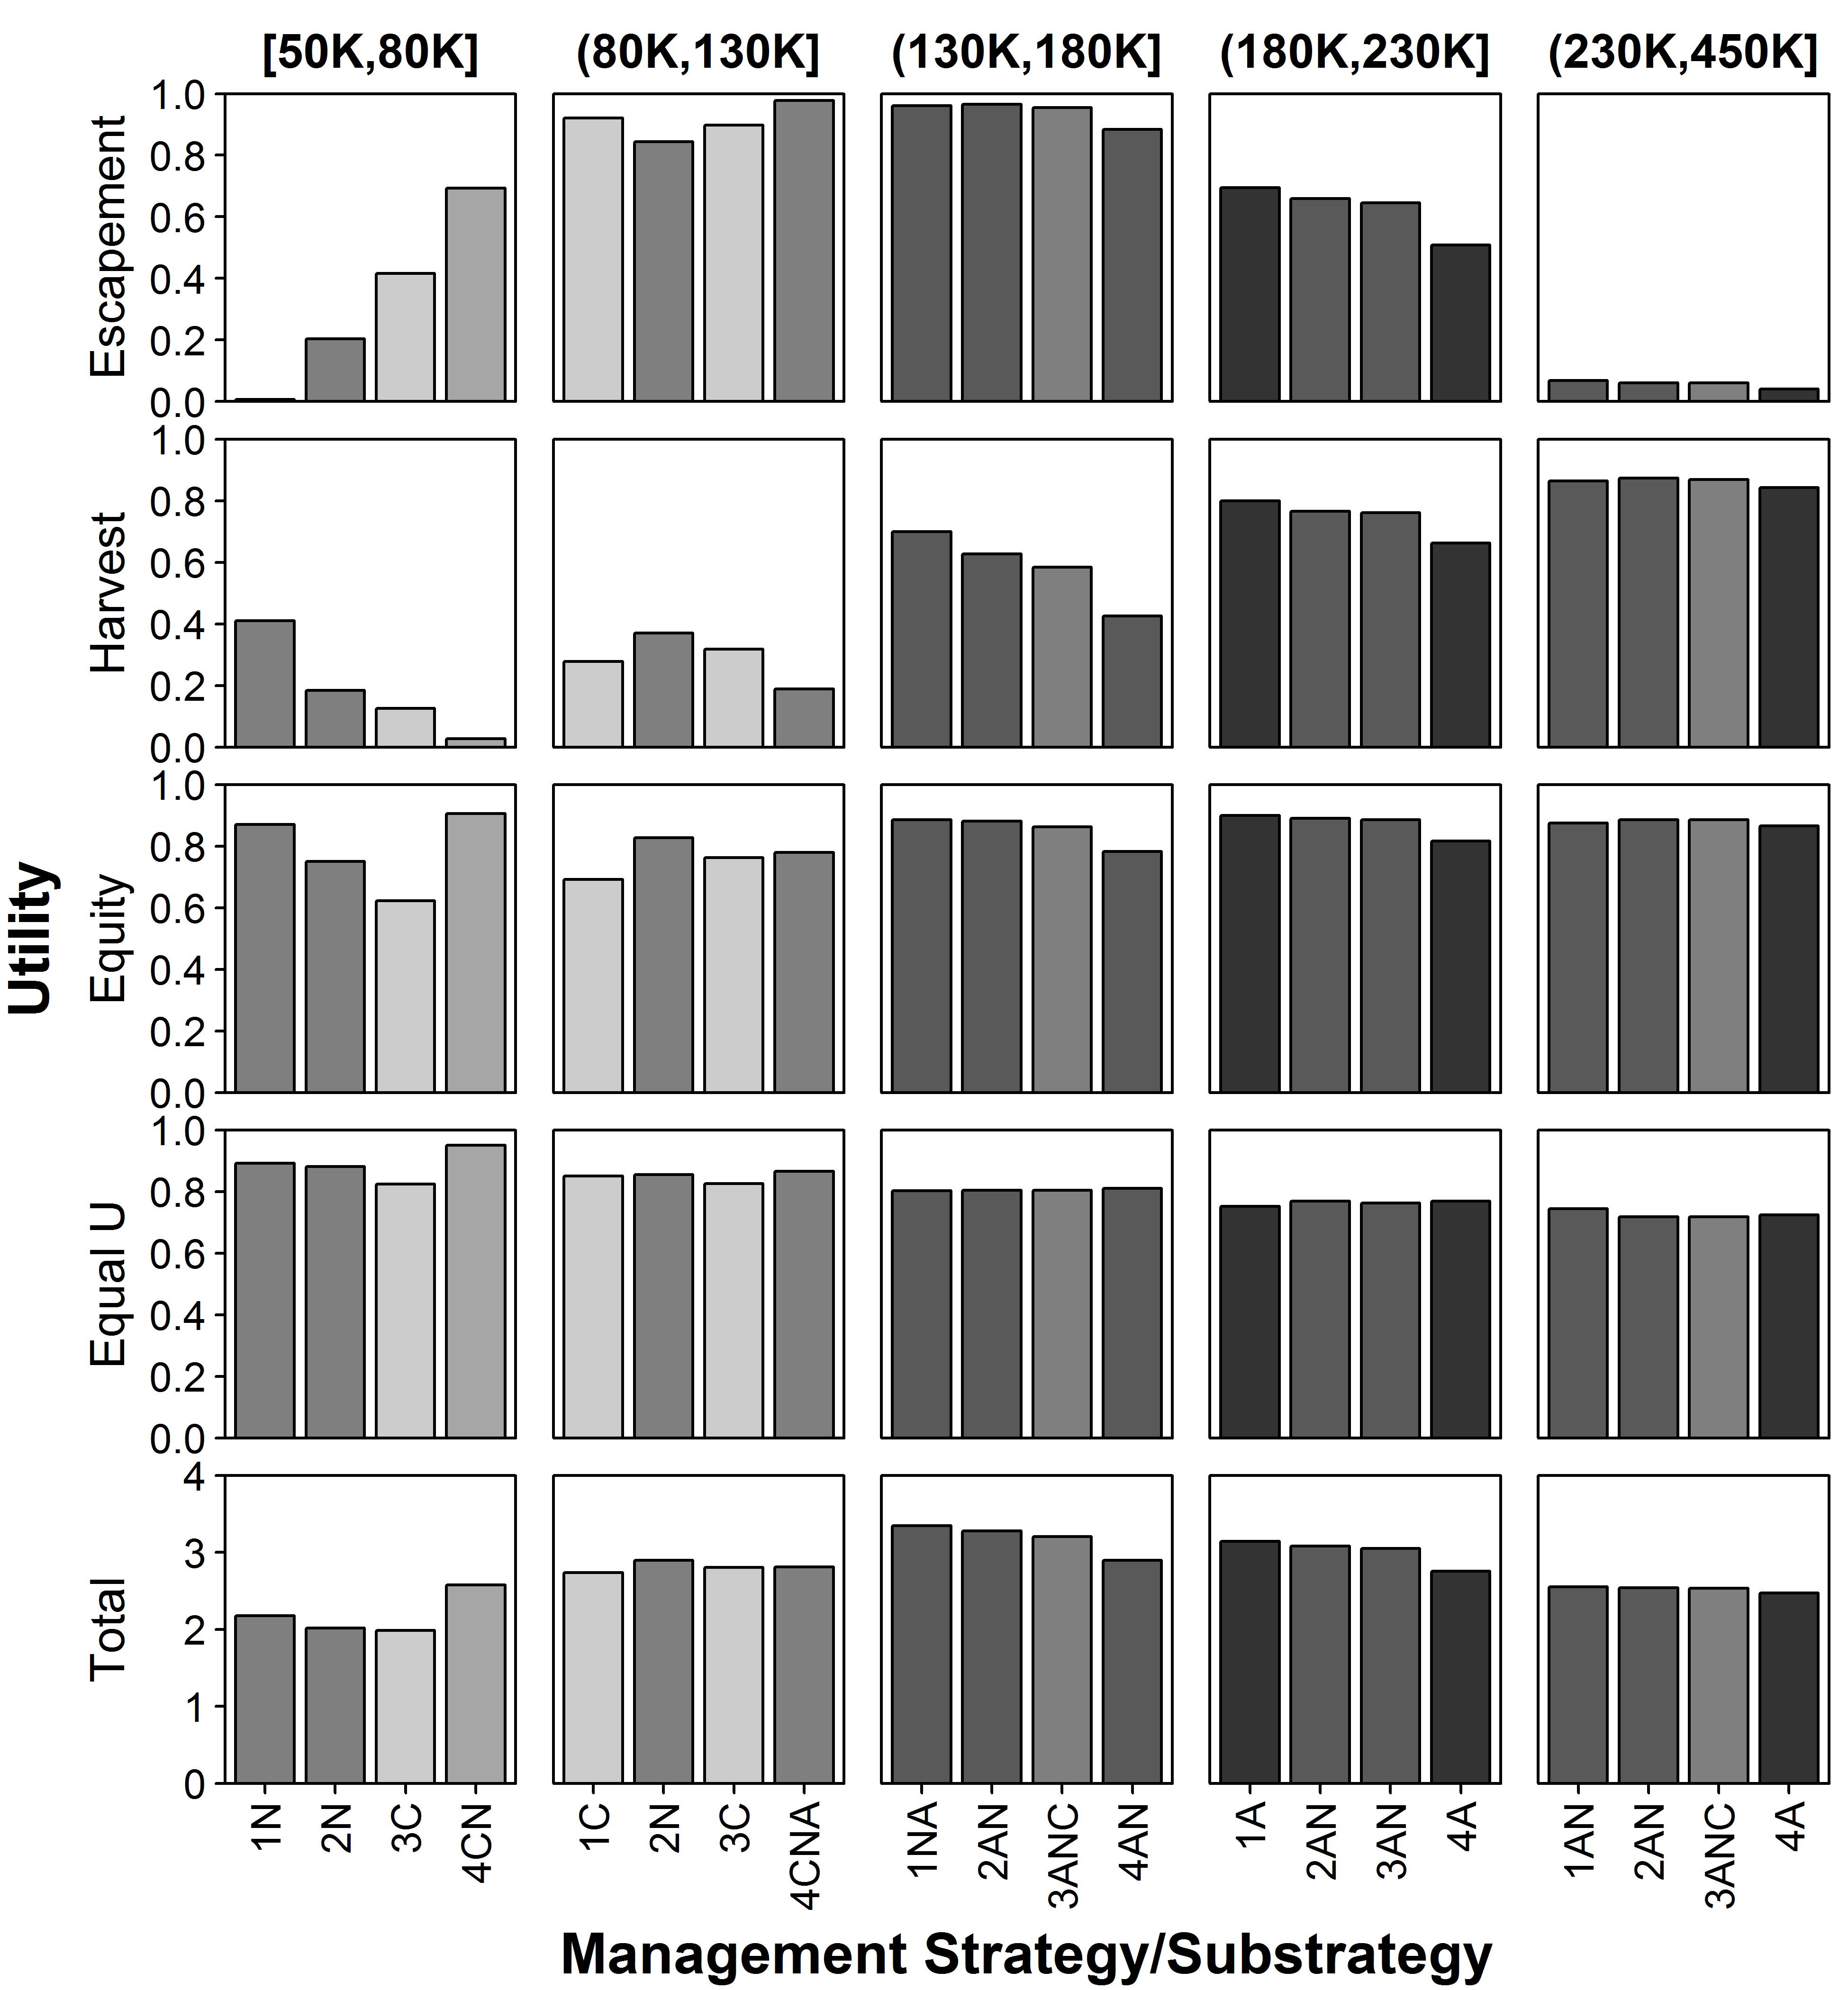
\includegraphics{img/Ch3/btwn-ms-utilities.jpg}
  \caption{Comparison of utility according to the different metrics between strategies (with the best substrategy selected for comparison) and run sizes. Numbers represent the strategy, letters and colors indicate the selected substrategy (darker colors represent more aggressive substrategies; C = conservative, N = neutral, A = aggressive; multiple letters indicate a tie). Total utility was calculated according to the default weighting scheme, where all objectives received equal weight.}
  \label{fig:btwn-ms-utilities}
\end{figure}

\begin{figure}
  \centering
  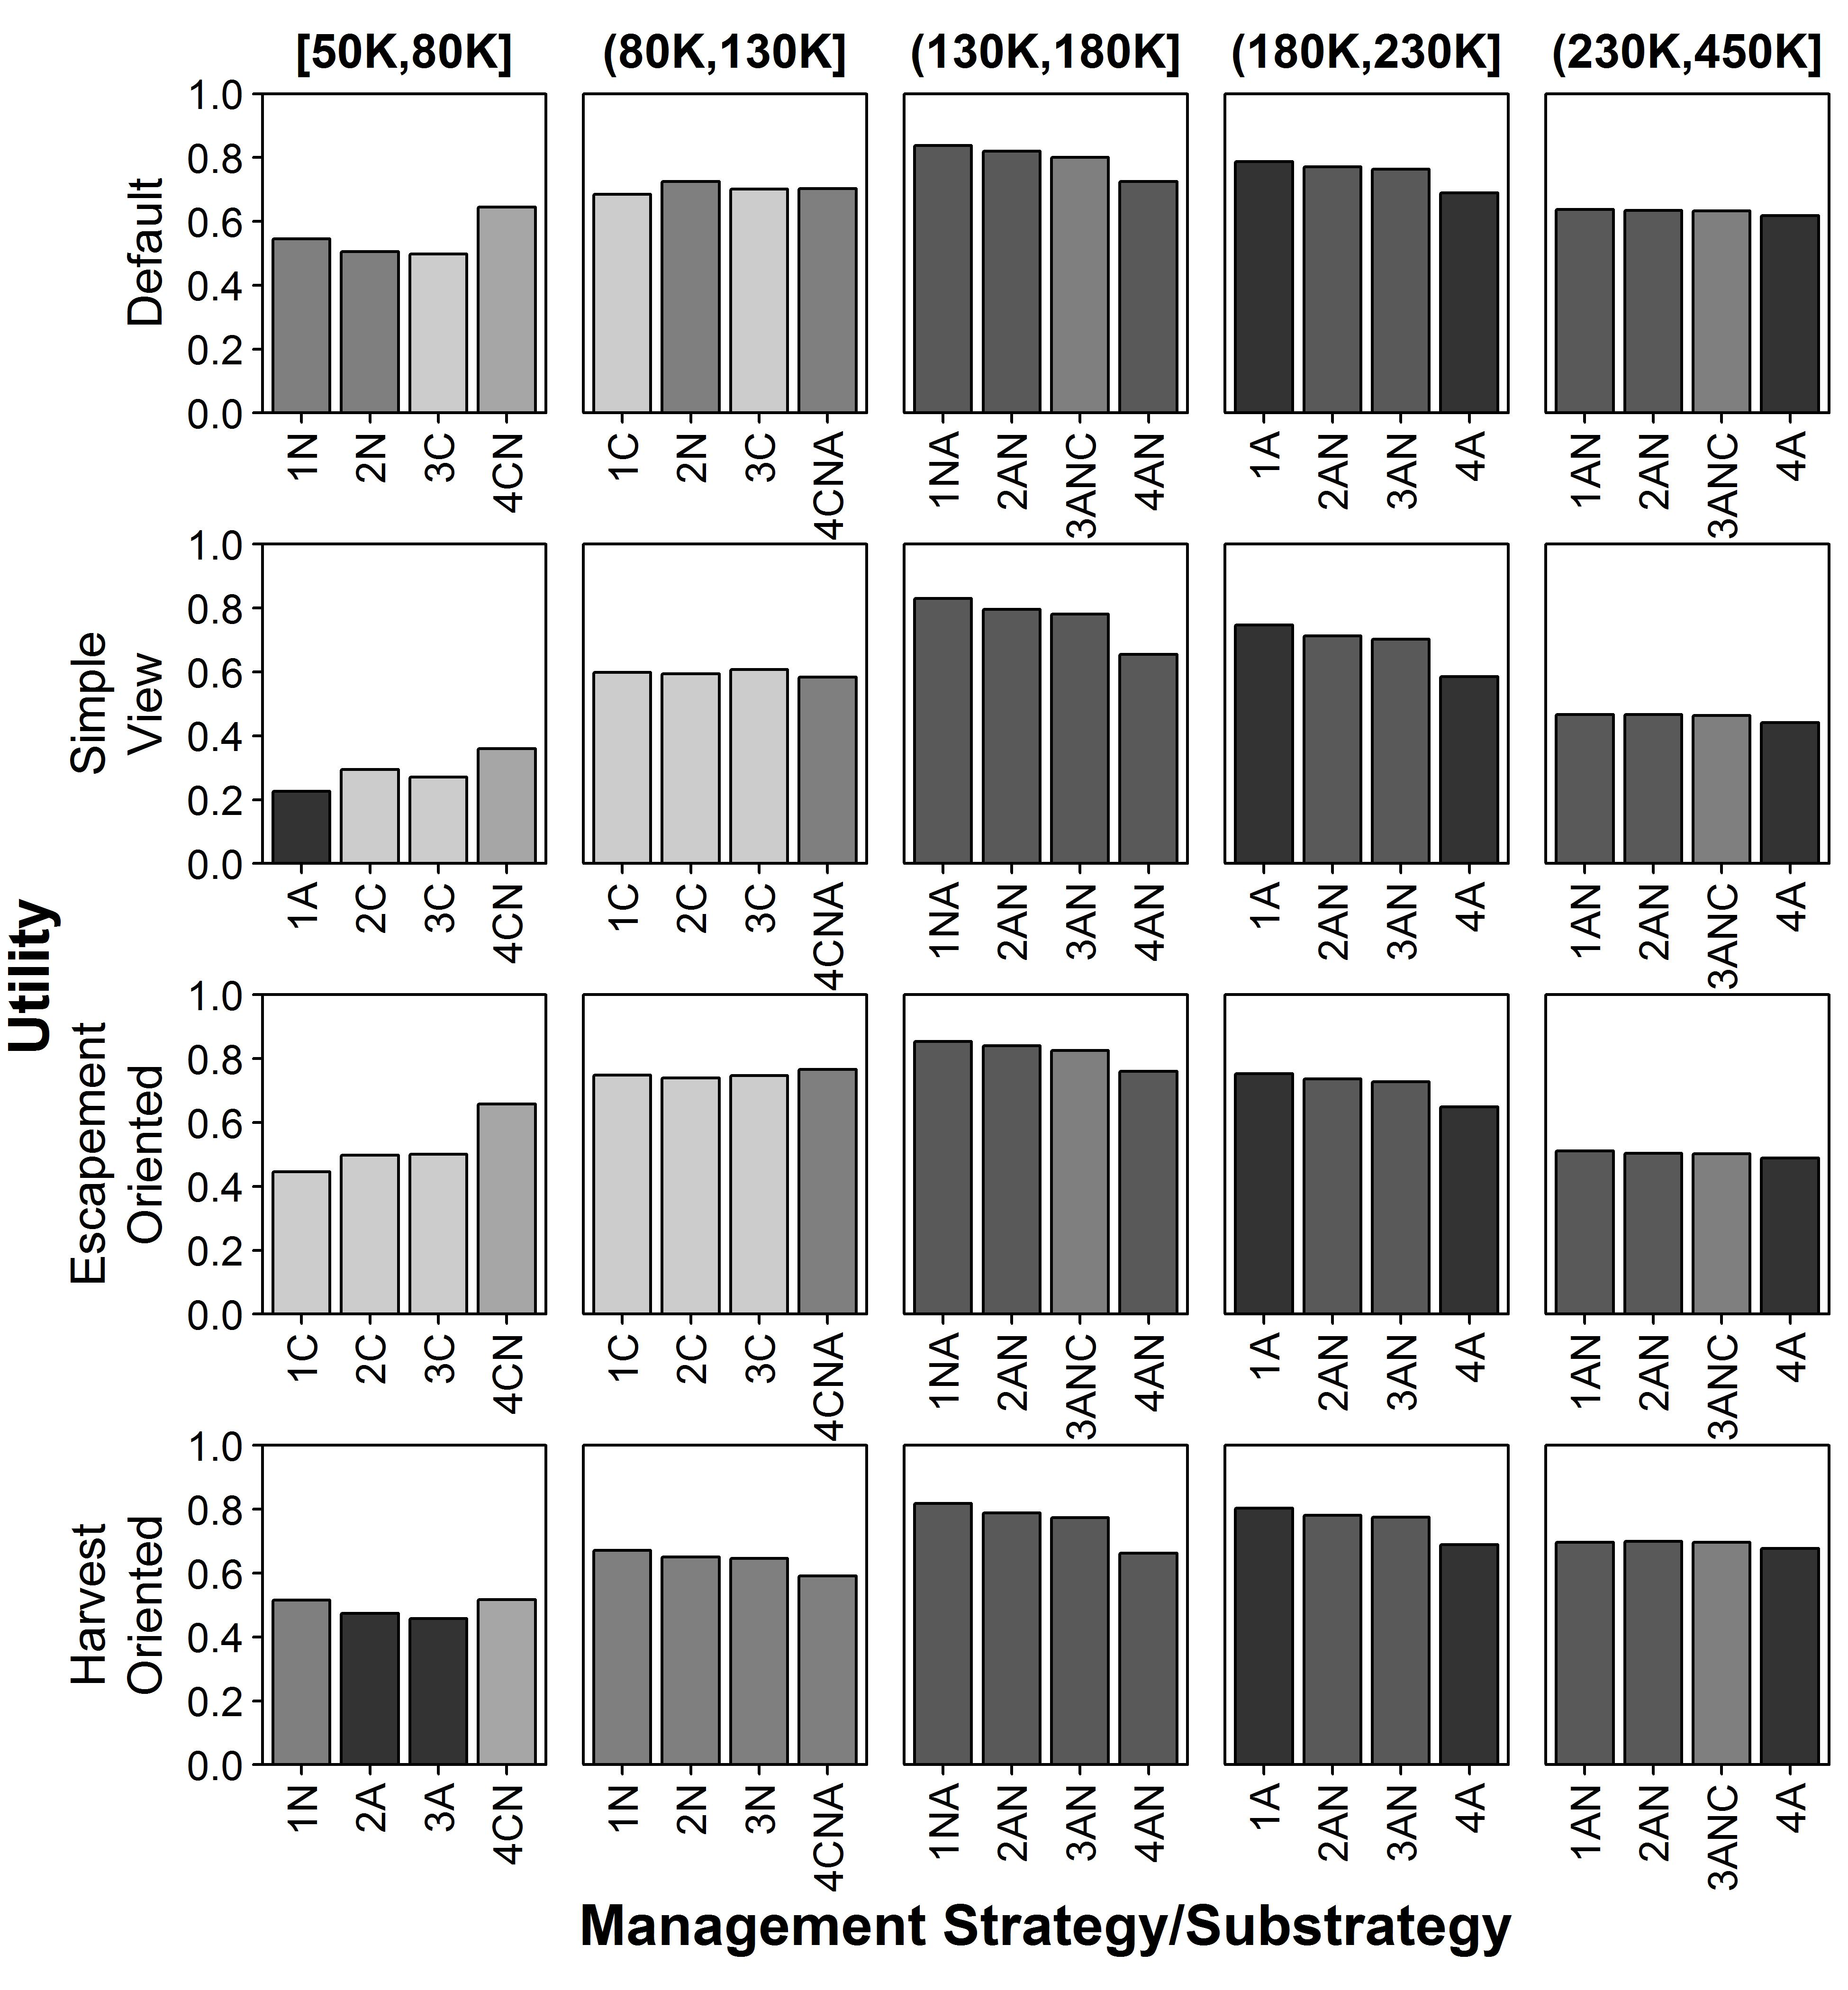
\includegraphics{img/Ch3/btwn-ms-weights.jpg}
  \caption{The total utility metric of the best-performing substrategy (letters/colors) for each strategy (numbers), when considering different weighting schemes (schemes described in Section \ref{alt-weights}). Bars are shaded based on the best substrategy, with darker greys representing more aggressive substrategies (C = conservative, N = neutral, A = aggressive; multiple letters indicate a tie). Total utility was scaled to the maximum attainable total utility for each weighting scheme, which is equal to the sum of the weights.}
  \label{fig:btwn-ms-weights}
\end{figure}

\end{singlespace}

\chapter{Assessment Approaches for Mixed-stock Pacific Salmon Fisheries:
Empirical and Simulation-Estimation Applications}\label{ch4}

\section*{Abstract}\label{abstract-2}
\addcontentsline{toc}{section}{Abstract}

\noindent
Although many salmon populations in large drainages are composed of many
smaller substocks, they are often managed and harvested as a
mixed-stock. There is likely to be heterogeneity in productivity among
the substocks, implying that some portion may need to be overfished if
the mixed-stock harvest is to be maximized, which constitutes a
trade-off. Methods to quantify substock productivity in the context
mixed-stock salmon fisheries are not well established, and fitting
substock-specific models independently may result in a loss of valuable
information. In this chapter, I develop an age-structured state-space
framework for simulateously fitting multiple spawner-recruit
relationships that allows for more complete use of available data and
sharing of information regarding recruitment anomalies experienced by
individual substocks. Four alternative state-space models were developed
and differed in their complexity in the treatment of recruitment and
maturity process error, and were compared to simpler regression-based
approaches. The models were fitted to reconstructed data from 13 Chinook
salmon substocks in the Kuskokwim River and estimation performance was
assessed using simulation-estimation trials. Biological and policy
conclusions were found to be largely consistent between different
state-space model structures, but differed strongly from the
regression-based approaches which suggested substantially more
aggressive harvest policies. The state-space framework was shown to be
largely unbiased when integrated across a range of true population
parameters, though strong biases were found for regression approaches.
The reliability and richness of biological inferences from the
state-space model suggest it shows promise for populating policy
evaluations directed at investingating the strength of
harvest-biodiversity trade-offs in mixed-stock salmon fisheries.

\section{Introduction}\label{introduction-2}

\noindent
Many salmon populations in large drainage systems are commonly harvested
in a relatively small spatial area and are managed as a single stock.
However, these ``stocks'' are instead stock-complexes, in which the
aggregate stock is comprised of several (and sometimes, many) substocks.
These substocks are known to show differences in genotypic
\citep{templin-etal-2004}, phenotypic \citep[e.g.,
morphology;][]{hendry-quinn-1997}, behavioral \citep[e.g., run
timing;][]{clark-etal-2015, smith-liller-2017a, smith-liller-2017b}, and
life history \citep[e.g., age-at-maturation,][]{blair-etal-1993}
characteristics that are the result of adaptations to local environments
after many generations of high spawning-site fidelity and reproductive
isolation from conspecifics in other tributaries located within the same
basin. It has been widely proposed that maintaining this diversity of
local adaptation (hereafter, ``biodiversity'') is favorable both from
ecosystem and exploitation perspectives. One argument is that in a
system where many parts contribute to the whole, the variability in the
aggregate characteristics can be dampened because of a lack of cohesion
in the subcomponent dynamics, a phenomenon known as the ``portfolio
effect'' \citep{schindler-etal-2010, schindler-etal-2015}.

Variability in substock-specific characteristics can ultimately lead to
heterogeneity in productivity among the substock components
\citep{walters-martell-2004}. Productivity in this context is the
ability of a population to replace itself after harvesting, often
represented for salmon populations as the maximum number of future
migrating adults (recruits) produced by one spawner (hereafter,
\(\alpha\)), which is attained at low spawner abundances due to
density-dependent survival. Substocks \(j\) with higher \(\alpha_j\)
values can sustain greater exploitation rates (\(U\)) than those with
smaller \(\alpha_j\) values, in fact, \(\alpha_j\) can be expressed in
terms of the exploitation rate that maximizes sustained yield from
substock \(j\) \citep[\(U_{\text{MSY},j}\);][]{schnute-kronlund-2002}:

\begin{equation}
  \alpha_j=\frac{e^{U_{\text{MSY},j}}}{1 - U_{\text{MSY},j}}.
  \label{eq:umsy-to-alpha}
\end{equation}

Given that there is likely some level of heterogeneity in \(\alpha_j\)
and \(U_{\text{MSY},j}\) among individual substocks, the logical
conclusion is that in a mixed-stock fishery where the exploitation rate
in year \(t\) (\(U_t\)) is common among all substocks, some weaker
substocks must be exploited at \(U_t > U_{\text{MSY},j}\) in order to
fish the more productive substocks at \(U_{\text{MSY},j}\). This of
course implies a trade-off, such that it may be necessary to
over-exploit some substocks in order to maximize harvest \citep[Figure
\ref{fig:trade-off-plot},][]{walters-martell-2004}.

Before these trade-offs can be considered by managers in a well-informed
way, the shape and magnitude of the trade-off must first be quantified
as shown in Figure \ref{fig:trade-off-plot}. Figures like this are
generated using the estimated productivity and carrying capacity of all
(or a representative sample) of the substocks within a mixed-stock
fishery. These quantities are obtained using a spawner-recruit analysis,
which involves tracking the number of recruits produced in each brood
year (i.e., parent year) by the number of fish that spawned in that same
year and fitting a curve to the resulting pattern. The spawner-recruit
literature is extensive, but focuses primarily on assessing single
populations as opposed to substock components \citep[but see the work on
Skeena River, British Columbia sockeye salmon \emph{O. nerka}
substocks;][]{walters-etal-2008, korman-english-2013}. Substock-specific
analyses are uncommon because of two factors: (1) the data to conduct
well-informed substock-specific spawner-recruit analyses are often
unavailable (20 -- 30 years of continuous spawner and harvest
counts/estimates and age composition for each substock) and (2)
management actions in large mixed-stock fisheries may not be dexterous
enough to deliberately exert higher exploitation rates on more
productive substocks, so deriving substock-specific estimates could be
of little utility. Regarding the former reason, there are some cases
where the data do exist to perform these kinds of analyses, however
methods to conduct multi-stock spawner-recruit analyses are not
well-developed. Regarding the latter, even in cases where management
cannot target particular substocks over others, understanding the nature
of the trade-offs can be informative for evaluating candidate harvest
policies for the mixed-stock in the context of substock biodiversity
\citep{walters-etal-2018}.

The methods to fit spawner-recruit models can be grouped into two broad
categories: regression-based approaches \citep[e.g.,][]{clark-etal-2009}
and state-space (i.e., time series) models
\citep[e.g.,][]{su-peterman-2012, fleischman-etal-2013}. The
regression-based approaches treat spawner-recruit pairs as independent
observations, and are thus subject to substantial pitfalls when dealing
with the inherent time-dependent properties and oftentimes large amounts
of observation error found in spawner-recruit data sets \citep[Ch.
7]{walters-martell-2004}. The consequence of ignoring the first issue is
the ``time-series bias'', which chronically causes positive biases in
\(\alpha\) and negative biases in \(\beta\), resulting in the same
directional biases in \(U_{\text{MSY}}\) and \(S_{\text{MSY}}\),
respectively \citep[i.e., spuriously providing too aggressive harvest
policy recommendations;][]{walters-1985}. The second is known as the
``errors-in-variables bias'' and is known to cause an apparent scatter
which inserts additional variability that commonly-used regression
estimators do not account for \citep{ludwig-walters-1981}. Though these
methods have been known for their problems for over 30 years, they are
still somewhat widely used \citep[e.g.,][]{korman-english-2013}. Unlike
the regression-based approaches, the state-space class of models
captures the process of recruitment events leading to future spawners
while simultaneously accounting for variability in the biological and
measurement processes that gave rise to the observed data
\citep{devalpine-hastings-2002, fleischman-etal-2013}. For these
reasons, state-space spawner-recruit analyses have been rapidly gaining
popularity, particularly in Alaska
\citep{su-peterman-2012, fleischman-etal-2013, staton-etal-2017-intseq}.
Including this level of additional model complexity comes at
computational costs, as these models are well-suited for Bayesian
inference with Markov Chain Monte Carlo (MCMC) methods \citep[Ch.
4]{newman-etal-2014}, but has been shown to reduce bias in estimates in
some circumstances \citep{su-peterman-2012, walters-martell-2004}.

In the Kuskokwim River Chinook salmon fishery, there has been recent
interest in considering biodiversity to explicitly inform the
drainage-wide escapement goal. In conducting the spawner-recruit
analysis to inform such policy analyses, it will be difficult to
determine which method is appropriate, given many possible model
structures, sparse data, and unknown sampling biases. Before strong
inferences can be made from the ultimate trade-off analyses of interest,
the performance of the estimation models used to parameterize them needs
to be evaluated, as well as the appropriate level of model complexity
needed to address the problem with sufficient accuracy. In this chapter,
I evaluate the performance of a range of assessment models for
mixed-stock salmon fisheries \emph{via} simulation-estimation and apply
them to Chinook salmon substocks in the Kuskokwim River as a case study.
The objectives were to:

\begin{enumerate}
\def\labelenumi{(\arabic{enumi})}
\item
  develop a set of varyingly complex multi-stock versions of state-space
  spawner-recruit models,
\item
  determine the sensitivity of biological and trade-off conclusions to
  assessment model complexity (including those obtained using
  regression-based approaches) using empirical data from Kuskokwim River
  Chinook salmon substocks, and
\item
  test the performance of the assessment models \emph{via}
  simulation-estimation trials.
\end{enumerate}

\section{Methods}\label{methods-2}

\noindent
This analysis was conducted in both an empirical and a
simulation-estimation framework to evaluate the sensitivity and
performance of assessment strategies for the mixed-stock assessment
problem in Pacific salmon fisheries. First, all assessment methods (two
regression-based and four state-space models) were fitted to observed
data from the Kuskokwim River substocks (\(n_j\) = 13) to determine the
extent to which the choice of assessment model structure might influence
biological and management conclusions. Then, a hypothetical exploited
system with known properties was simulated and was composed of several
age-structured substocks. Then, these hypothetical populations were
sampled per a realistic sampling scheme and each of the assessment
models were fitted to the resulting data sets. Estimation performance
regarding quantities used in management (e.g., \(U_{\text{MSY}}\) and
\(S_{\text{MSY}}\)) was calculated from the resulting estimates.
Inference from the simulation can then be used to justify an appropriate
level of model complexity.

\subsection{Multi-stock spawner-recruit models}\label{model-methods}

\subsubsection{Regression-based models}\label{reg-methods}

\noindent
Two regression-based approaches to estimating \citet{ricker-1954}
spawner-recruit parameters in the multi-stock case were assessed: (1) a
single mixed-effect regression model with random intercepts and (2)
independent regression models. The \citet{ricker-1954} spawner-recruit
model can be written as:

\begin{equation}
  R_y=\alpha S_y e^{-\beta S_y + \varepsilon_y}
  \label{eq:basic-ricker}
\end{equation}

\noindent
where \(R_y\) is the total recruitment produced by the escapement
\(S_y\) in brood year \(y\), \(\alpha\) is the maximum expected
recruits-per-spawner (RPS), \(\beta\) is the inverse of the escapement
that is expected to produce maximum recruitment (\(S_{\text{MAX}}\)),
and \(\varepsilon_y\) are independent mean zero random variables
attributed solely to environmental fluctuations. Primary interest lies
in estimating the population dynamics parameters \(\alpha\) and
\(\beta\) as they can be used to obtain biological reference points off
of which sustainable harvest policies can be developed. This function is
increasing at small escapements and declining at large ones, though can
be linearized:

\begin{equation}
  \log(\text{RPS}_y)=\log(\alpha)-\beta S_y + \varepsilon_y,
  \label{eq:lin-ricker-fixed}
\end{equation}

\noindent
allowing for estimation of the parameters log(\(\alpha\)) and \(\beta\)
in a linear regression framework using the least squares method
\citep{hilborn-walters-1992, clark-etal-2009}. This relationship is
nearly always declining, implying a compensatory effect on survival
(i.e., RPS) with reductions in spawner abundance \citep{rose-etal-2001}.

A multi-stock formulation of this model can be formulated by including
substock-specific random effects on the intercept {[}log(\(\alpha\)){]}:

\begin{equation}
  \begin{split}
    \log(\text{RPS}_{y,j})=\log(\alpha_j)-\beta_j S_{y,j} + \varepsilon_y, \\
    \log(\alpha_j)=\log(\alpha) + \varepsilon_{\alpha,j}, \\
    \varepsilon_{\alpha,j} \sim \text{N}(0,\sigma_{\alpha}). \\
  \end{split}
\label{eq:lin-ricker-mixed}
\end{equation}

\noindent
It does not make sense to include substock-level random effects on the
slope, given that \(\beta\) is a capacity parameter related to the
compensatory effect of resource limitation experienced by juveniles,
likely in the freshwater environment (i.e., amount of habitat as opposed
to quality of habitat). Fitting the individual substock models in this
hierarchical fashion allows for the sharing of information such that the
more intensively-assessed substocks can help inform those that are more
data-poor.

The mixed-effect model may have the benefit of sharing information to
make some substocks more estimable, but it should also have the tendency
to pull the extreme \(\alpha_j\) (those in the tails of the
hyperdistribution) toward \(\alpha\). This behavior may not be
preferable for policy recommendations, as it should tend to dampen the
extent of heterogeneity estimated in \(\alpha_j\). For this reason,
independent regression estimates for each substock were also obtained
for evaluation. In estimating the parameter \(\log(\alpha)\), a lower
bound constraint of 0 was used in all regression models. This was
necessary to prevent the models from estimating biologically-implausible
parameters: if \(\log(\alpha)\) \textless{} 0, then the stock would
produce \textless{} 1 RPS at its most productive state, in which case it
would likely not currently be in existence.

\subsubsection{State-space models}\label{ssm-model}

\noindent
Four versions of the state-space formulation were developed. As three
versions were simplifications of the full model, the full model is
presented completely here and the changes resulting in the other three
model structures are described following the description of the full
model.

The state-space formulation of a multi-stock spawner-recruit analysis
developed and evaluated here is an extension of various single-stock
versions \citep[e.g.,][]{fleischman-etal-2013}.
\citet{walters-etal-2008} used a similar model using maximum likelihood
methods to provide estimates of \textgreater{}50 substocks in the Skeena
River drainage, British Columbia. The model presented here was fitted in
the Bayesian mode of inference using program JAGS \citep{plummer-2017},
and allows for relaxation of certain assumptions made by
\citet{walters-etal-2008} such as the important notion of
perfectly-shared recruitment residuals (i.e., anomalies -- deviations
from the expected population response). It also has the ability to relax
the assumption of constant maturity schedules across brood years.

The state-space model is partitioned into two submodels: (1) the process
submodel which generates the true states of \(R_{y,j}\) and the
resulting calendar year states (e.g., \(S_{t,j}\)) and (2) the
observation submodel which fits the true states to the observed data
(Table \ref{tab:ch4-notation-table}). Note that this method allows for
missing calendar year observations and does not require excluding brood
year recruitment events that were not fully-observed as was necessary
for the regression-based models (see Appendix \ref{lm-btable}).

The recruitment process operated by producing a mean prediction from the
deterministic \citet{ricker-1954} relationship \eqref{eq:basic-ricker} for
\(n_y\) brood years for each of the \(n_j\) substocks. From these
deterministic predictions, auto-correlated process variability was added
to generate the true realized state. To populate the first \(n_a\)
calendar year true states with recruits of each age \(a\), the first
\(a_{max}\) brood year expected recruitment states were not linked to a
spawner abundance through \eqref{eq:basic-ricker} (because the \(S_y\)
component was not observed), but instead were assumed to have a constant
mean equal to the unfished equilibrium recruitment (where non-zero
\(S_j\) produces \(R_j = S_j\) when unexploited and in the absence of
process variability):

\begin{equation}
  \bar{R}_{y,j}=\frac{\log(\alpha_j)}{\beta_j},
  \label{eq:unfished-R0}
\end{equation}

\noindent
where \(\bar{R}_{y,j}\) is the expected (i.e., deterministic)
recruitment in brood year \(y\) from substock \(j\) with Ricker
parameters \(\alpha_j\) and \(\beta_j\). The remaining \(n_y - a_{max}\)
brood years had an explicit time linkage:

\begin{equation}
  \bar{R}_{y,j} = \alpha_j S_{t,j} e^{-\beta_j S_{t,j}},
  \label{eq:tsm-ricker-pred}
\end{equation}

\noindent
where \(t = y-a_{max}\) is the \(t^{\text{th}}\) calendar year index in
which the escapement produced the recruits in the \(y^{\text{th}}\)
brood year index.

From these deterministic predictions of the biological recruitment
process, lag-1 auto-correlated process errors were added to produce the
true realized states:

\begin{equation}
  \log(R_{y,1:n_j}) \sim \text{MVN}\left(\log(\bar{R}_{y,1:n_j}) + \omega_{y,1:n_j}, \Sigma_R\right),
  \label{eq:tsm-ricker-anomalies}
\end{equation}

\noindent
where

\begin{equation}
  \omega_{y,1:n_j} = \phi \left(\log(R_{y-1,1:n_j}) - \log(\bar{R}_{y-1,1:n_j}) \right),
  \label{eq:tsm-omega}
\end{equation}

\noindent
and \(R_{y,1:n_j}\) is a vector of true recruitment states across the
\(n_j\) stocks in brood year \(y\), \(\omega_{y,1:n_j}\) is the portion
of the total process error attributable to serial auto-correlation,
\(\phi\) is the lag-1 auto-correlation coefficient (constant across
substocks), and \(\Sigma_R\) is a covariance matrix representing the
white noise portion of the total recruitment process variance.
\(\Sigma_R\) was estimated such that each substock was assigned a unique
variance and covariance with each other substock. This was achieved by
using an inverse Wishart prior distribution, with degrees of freedom
equal to \(n_j + 1\) and the scale matrix populated with zero-value
elements along the off-diagonals and 1 along the diagonal elements,
which inserts little information about the covariance matrix
\(\Sigma_R\) \citep{plummer-2017}. The multivariate normal errors were
on the logarithmic scale so the variability on \(R_{y,j}\) was
lognormal, which is the most commonly used error distribution for
describing spawner-recruit data sets \citep{walters-martell-2004}.
Further, the multivariate normal was used as opposed to \(n_j\) separate
normal distributions so the degree of synchrony in brood year
recruitment deviations (i.e., recruitment process errors) among
substocks could be captured and freely estimated.

The maturity schedule is an important component of age-structured
spawner-recruit models, as it determines which calendar years the brood
year recruits \(R_{y,j}\) return to spawn (and be observed). Recent
state-space spawner-recruit analyses have accounted for brood year
variability in maturity schedules as Dirichlet random vectors drawn from
a common hyperdistribution characterized by a mean maturation-at-age
probability vector (\(\pi_{1:n_a}\)) and an inverse dispersion parameter
(\(D\)) \citep[see][ for implementation in
JAGS]{fleischman-etal-2013, staton-etal-2017-intseq}, and the same
approach was used here with maturity schedules shared perfectly among
substocks within a brood year. Brood year-specific maturity schedules
were treated as random variables such that:

\begin{equation}
  p_{y,a} \stackrel{\text{iid}}{\sim} \text{Dirichlet}(\pi_{1:n_a} D). 
  \label{eq:dirichlet}
\end{equation}

\noindent
where \(p_{y,a}\) is the probability a fish spawned in brood year \(y\)
will mature at age \(a\).

In order to link \(R_{y,j}\) with calendar year observations of
escapement from each substock, \(R_{y,j}\) was allocated to calendar
year runs-at-age (\(N_{t,a,j}\)) based on the maturity schedule:

\begin{equation}
  N_{t,a,j} = R_{t+n_a-a,j} p_{t+n_a-a,a},
  \label{eq:tsm-get-N-ta}
\end{equation}

\noindent
and the total run returning to substock \(j\) in year \(t\) was the sum
across ages:

\begin{equation}
  N_{t,j}=\sum_{a=1}^{n_a} N_{t,a,j}.
  \label{eq:tsm-get-N}
\end{equation}

\noindent
The harvest process was modeled using a freely estimated annual
exploitation rate (\(U_t\)) time series, which was assumed to apply
equally to all substocks:

\begin{equation}
  H_{t,j}=N_{t,j} U_t,
  \label{eq:tsm-get-H}
\end{equation}

\noindent
and escapement was obtained as:

\begin{equation}
  S_{t,j}=N_{t,j} (1 - U_t).
  \label{eq:tsm-get-S}
\end{equation}

The quantity \(H_t\) aggregated among all substocks was obtained by
summing \(H_{t,j}\) within a \(t\) index across the \(j\) indices. The
true age composition returning in year \(t\) to substock \(j\)
(\(q_{t,a,j}\)) was obtained as:

\begin{equation}
  q_{t,a,j} = \frac{N_{t,a,j}}{N_{t,j}}.
  \label{eq:get-q}
\end{equation}

Three data sources were used to fit the model: (1) observed escapement
from each substock (\(S_{obs,t,j}\)) with assumed known coefficients of
variation (CV), (2) total harvest arising from the aggregate stock
(\(H_{obs,t}\)) with assumed known CV, and (3) the age composition of
substocks with these data each calendar year (\(q_{obs,t,a,j}\); which
had associated effective sample size \(ESS_{t,j}\) equal to the number
of fish successfully aged for substock \(j\) in year \(t\)). The CVs
were converted to lognormal standard deviations:

\begin{equation}
  \sigma_{\text{log}}=\sqrt{\log(\text{CV}^2+1)},
  \label{eq:cv2sig}
\end{equation}

\noindent
and used in lognormal likelihoods to fit the time series \(S_{t,j}\) to
\(S_{obs,t,j}\) and \(H_t\) to \(H_{obs,t}\). Calendar year age
composition was fitted using multinomial likelihoods with parameter
vectors \(q_{t,1:n_a,j}\) and observed vectors of
(\(q_{obs,t,1:n_a,j} ESS_{t,j}\)).

Three alternative formulations of the state-space model were evaluated,
and all were simplifications of the full model described above regarding
the structure of (1) the covariance matrix on recruitment residuals and
(2) the maturity process (see Table \ref{tab:models-table} for a
summary). The simplest model did not include brood year variability in
maturity schedules and \(\Sigma_R\) was constructed by estimating a
single \(\sigma_R^2\) and \(\rho\), and populating the diagonal elements
with \(\sigma_R^2\) and off-diagonal elements with \(\rho \sigma_R^2\).
This simplest model is denoted as SSM-vm throughout the rest of this
chapter. One drawback of constructing \(\Sigma_R\) this way is that
\(\rho < -0.05\) for a \(13 \times 13\) covariance matrix results in
positive-indefiniteness, which is prohibited by JAGS
\citep{plummer-2017}. Thus, a constraint was required to maintain
\(-0.05 \le \rho < 1\) to prevent the sampler from crashing. In one
intermediate model (SSM-vM), brood year maturation variability was
included but the covariance matrix was constructed as in the simplest
model. In the other intermediate model (SSM-Vm), brood year variability
in maturation was not included but the covariance matrix was fully
estimated as in the full model (SSM-VM). As for the choice of notation,
lowercase letters indicate the simple version of a structure and
uppercase letters indicate the complex structure; ``v'' refers to
recruitment covariance structure and ``m'' refers to maturity. I chose
these two structural uncertainties (complexity in recruitment covariance
and maturity variability) for evaluation here because I thought them to
be two key areas where an analyst might question if the available data
are adequate for model fitting and inference. In other words, these are
two key structural uncertainties where it is important to know if the
complex versions are reliably estimable with a reasonable amount of
data.

\subsection{Kuskokwim empirical
analysis}\label{kuskokwim-empirical-analysis}

\subsubsection{Study system}\label{study-system}

\noindent
All six assessment models (two regression-based and four state-space
models) developed in this chapter were fitted to empirical data from
Chinook salmon substocks of the Kuskokwim River located in western
Alaska (Figure \ref{fig:ch4-map}). The Kuskokwim River salmon fishery
can very well be described as a mixed-stock fishery, both for multiple
salmon species (predominately Chinook, chum \emph{O. keta}, and sockeye
salmon) and for multiple substocks of the same species. Fish originating
from and returning to the various tributaries enter through the bulk of
the fishery as a mixed-stock, though Chinook salmon stocks traveling to
the headwaters have been illustrated to enter the main stem earliest in
the summer migration \citep{smith-liller-2017a, smith-liller-2017b} so a
limited ability to direct harvest toward or away from these substocks is
possible by manipulating the front portion of the fishery (Chapter
\ref{ch3}, this dissertation). It is acknowledged that the assessment
program does not sample all tributaries within the Kuskokwim River where
Chinook salmon spawn, but total run size between 1976 -- 2017 has been
estimated \emph{via} run reconstruction \citep{liller-etal-2018}.

\subsubsection{Data sources}\label{data-sources}

\noindent
The data set used included counts of Chinook salmon at many locations
throughout the Kuskokwim River system (Figure \ref{fig:ch4-map}). Nearly
all data were collected by projects managed by the Alaska Department of
Fish and Game (ADF\&G) and a complete description of data needs and
preparation procedures is provided in Appendix \ref{appendix-c}. The raw
escapement data set available spanned 20 different escapement monitoring
projects (six weirs and 14 aerial surveys) and 42 calendar years from
1976 -- 2017; see \citet{head-smith-2018} for details on tributary
escapement monitoring. Some pre-processing was required to convert the
aerial survey index counts to estimates of total spawners (Appendix
\ref{air-expansion}). Annual estimates of Chinook salmon harvest
originating from both subsistence and commercial fisheries in each year
was also available, as was the estimated exploitation rate of the
aggregate stock (details in Appendix \ref{harv-expansion}). Finally, age
composition data were available for the six substocks monitored
\emph{via} weir programs (details in Appendix \ref{age-comp}).

\subsubsection{Sensitivity Analyses}\label{sensitivity-analyses}

\noindent
Two sensitivity analyses were conducted to test the robustness of
inference from the state-space models with the Kuskokwim data. First,
the default assumption that all substocks have been fished at the same
rate each year is tenuous. I included a term in the model that allowed
for substocks to have differential vulnerability (\(v_j\)) by replacing
\(U_t\) with \(U_tv_j\) in \eqref{eq:tsm-get-H} and \eqref{eq:tsm-get-S}
which makes an adjustment that acknowledges some substocks experienced
higher exploitation rates than others. This alteration changes the
interpretation of the parameter vector \(U_t\) to be the exploitation
rate of fully-vulnerable substocks. Without additional information on
what portion of \(H_{obs,t}\) was attributable to each substock going
back in time, the \(v_j\) elements are not estimable. In the absence of
this information for Kuskokwim River Chinook salmon, the value of the
vulnerability parameters was set by calculating the fraction of the
fishing households along the main-stem of the river that each substock
must travel past in order to reach their natal spawning grounds. Fishing
household data were available from post-season interviews conducted by
ADF\&G \citep[e.g.,][]{hamazaki-2011, shelden-etal-2016b}\footnote{These
  data were the same as those used in Chapter \ref{ch3} of this
  dissertation when determining the spatial distribution of fishing
  effort and salmon needs in the management strategy evaluation
  operating model.}. Although this method ignores the temporal overlap
of the fishery \citep{hamazaki-2008} with the arrival timing of
particular substock groups
\citep{smith-liller-2017a, smith-liller-2017b}, it was intended as a
first step at determining how much the conclusions might depend on how
the internal harvest accounting was specified. No attempt was made to
alter how harvest was apportioned for use in the regression-based
models.

As a secondary sensitivity analysis, the information content of the age
composition data was reduced. In the default case, each annual
multinomial age composition vector was weighted by the number of fish
successfully aged for that substock/year combination. For some
substocks/years, this number was quite high from a multinomial sampling
perspective when the number of categories is small (e.g., \(\approx\)
1,200 samples across four age categories). To assess whether this
strength of information had an impact on the inference, I manipulated
the effective sample size such that the maximum number of fish sampled
for a substock was assigned \(ESS_{t,j}\) = 100, and the other years
with data were scaled proportionately.

\subsubsection{Comparisons of model
output}\label{comparisons-of-model-output}

\noindent
Key population dynamics parameters and biological reference points were
compared between six assessment models wherever possible to determine
the extent to which the management conclusions might change based on the
model structure used. Where appropriate, quantities were averaged across
substocks to facilitate comparisons and included indicators of the
average substock's productivity (\(\bar{\alpha}_j\) and
\(\bar{U}_{\text{MSY},j}\)) and size (\(\bar{S}_{\text{eq},j}\),
\(\bar{S}_{\text{MSY},j}\), and \(\bar{S}_{\text{MAX},j}\)). Reference
points for the aggregate mixed-stock included \(U_{\text{MSY}}\) and
\(S_{\text{MSY}}\) and a set of metrics that incorporate biodiversity
aspects as well: \(S^*_p\) \(H^*_p\), and \(U^*_p\), which represent the
mixed-stock escapement, harvest, or exploitation rate, respectively,
that would ensure no more than \(p \cdot 100\%\) of substocks would be
overfished, defined here as the case where a substock would be fished at
\(U > U_{\text{MSY},j}\). Three levels of \(p\) were extracted: 0.1,
0.3, and 0.5.

Model fits to the data (\(S_{obs,t,s}\), \(H_{obs,t}\), and
\(q_{obs,t,a,j}\)) were examined for all state-space models and
noteworthy differences between model structures were identified.
Estimates of synchrony in recruitment anomalies were examined, both
between two average substocks (\(\bar{\rho}_{i,j}\)), and between all
substock pairs. For the simple recruitment variance models (SSM-vm and
SSM-vM), correlations between each substock pair were conducted by
applying Pearson's \(r\) coefficient to two substocks' estimated
recruitment anomaly time series; in the complex variance models these
correlations were captured in the freely-estimated covariance matrix,
and they were extracted and summarized. Although the state-space models
were ignorant of the spatial relationships between the substocks,
comparisons were made to determine if substocks closer in proximity
showed higher synchrony than those spaced more distantly, as might be
expected. The auto-correlation parameter (\(\phi\)) and characteristics
of the maturity schedules (\(\pi_a\) and \(D\)) were also compared
between state-space models.

Harvest-biodiversity trade-offs were visualized in two ways. First, the
equilibrium aggregate mixed-stock escapement and harvest were
calculated\footnote{Equilibrium equations for the \citet{ricker-1954}
  model can be found in Table 2 of \citet{schnute-kronlund-2002} for the
  case where \(\gamma = 0\).} at each level of a mixed-stock
exploitation rate that affected all substocks equally. The fraction of
substocks overfished and trending towards extirpation (defined as the
case where equilibrium \(S_{j} \leq 0\)) were also calculated. As a
secondary, possibly more direct trade-off visualization, the fraction of
substocks overfished and trending towards extirpation was plotted
against the fraction of the mixed-stock MSY obtained at each
exploitation rate.

Some substocks could not be fitted using the regression approach because
they had fewer than three observed pairs of \(\text{RPS}_{y,j}\) (see
Appendix \ref{lm-btable} for details). When comparing quantities to the
estimates from the state-space models, the substocks that could not be
fitted with the regression approaches were removed from the state-space
model outputs. When comparisons were made between state-space models
only, these substocks were retained.

\subsection{Simulation-estimation
trials}\label{simulation-estimation-trials}

\noindent
To test the performance of these models, I created 160 hypothetical
salmon data sets designed to mimic the Kuskokwim River empirical data
set. I attempted to fit each of the six assessment models described in
Section \ref{model-methods} to each data set.

Given that the state-space model is a much more natural model of this
system (which has intrinsic time series properties) than the
regression-based versions, it was used as the foundation of the
operating model (i.e., state-generating model). The biological submodel
was more complex than the most complex estimation model -- namely with
regards to the maturity schedule, which had a modest level of substock
variability in mean maturity but with highly correlated brood year
variability; see Appendix \ref{appendix-d} for details. In order to
serve as the state-generating model for the simulation, the state-space
model needed only to be populated with true parameters, initial states,
and a harvest control rule. A fixed exploitation rate policy was used
(chosen to maximize yield without overfishing more than 30\% of the
substocks) with a modest amount of implementation error to ensure the
data time series were generated with enough contrast in spawner
abundance. \(n_j\) = 13 substocks were simulated with different
parameters \(U_{\text{MSY},j}\) and \(S_{\text{MSY},j}\) which took on
the values of random posterior draws from the most complex state-space
model fitted to the Kuskokwim River Chinook salmon substock data. All
other parameters were chosen to mimic the estimated values from the
Kuskokwim analysis, with the exception of \(\Sigma_R\), which was set to
have a modest amount of substock recruitment variability
(\(\bar{\sigma}_{j,j} \approx 0.4\)); \(\rho_{i,j}\) for each pair of
substocks was simulated randomly between -1 and 1, but approximately 0
when averaged across all substocks.

For a given set of simulated true states, a set of observed states
(\(S_{obs,t,j}\), \(H_{obs,t}\), \(q_{obs,t,a,j}\)) was generated by
adding sampling error to each year, which represented the value that
would have been observed if the sampling project operated that year.
Observation errors in escapement and harvest estimates were lognormal
and multinomial for the age composition, as assumed in the state-space
estimation model. Frequency of sampling on each substock (i.e.,
simulated data collection) was set to approximately mimic the Kuskokwim
River historical monitoring program (Figure \ref{fig:obs-freq}). The
sampling frequency was designed to continue to generate sampling
schedules until one was found that ensured no substock had fewer than
three observations of \(\text{RPS}_{y,j}\) which allowed the
regression-based models to include all substocks. Aggregate harvest
(\(H_{obs,t}\)) was assumed to be available every year in each
simulation and it was assumed that the exploitation rate could be
estimated in an unbiased fashion.

Estimation performance in terms of accuracy between assessment models
was calculated using the proportional error
(\(\frac{x_{\text{est}} - x_{\text{true}}}{x_{\text{true}}}\)), and the
central tendency and variability between random data sets were
visualized using boxplots. Key quantities of interest for comparison
between the regression approaches and the state-space models included:
\(S_{\text{MSY}}\), \(U_{\text{MSY}}\), \(S^*_p\), \(U^*_p\),
\(\alpha_j\), \(U_{\text{MSY},j}\), and \(S_{\text{MSY},j}\). For the
state-space models, the ability to accurately estimate the abundance
states of \(R_{y,j}\), \(S_{t,j}\), and \(H_{t}\) was also assessed,
summarized for early years and all years separately to investigate the
influence of the assumption that the observation time series began at
unfished equilibrium, as described by \eqref{eq:unfished-R0}. Credible
interval coverage at the 95\% level was assessed by determining the
fraction of obtained credible intervals included the true value.
Additionally, model run times and convergence diagnostics were
summarized for all models that successfully fitted the simulated data
sets.

\subsection{Computation}\label{computation}

\noindent
All parameter estimation was conducted in the Bayesian framework using
the MCMC engine JAGS \citep{plummer-2017} invoked through R
\citep{r-cite} using the package \texttt{\{jagsUI\}} \citep{r-jagsUI}.
All priors for the regression-based methods (Table
\ref{tab:lm-prior-table}) and state-space models (Table
\ref{tab:ssm-prior-table}) were selected to be as minimally-informative
as possible, while still preventing the MCMC sampler from exploring
highly unlikely areas of the parameter space. I wrote two packages to
simplify the workflow of this analysis\footnote{For reference, any of
  the packages I wrote for this analysis can be installed on any R
  user's computer by executing:
  \texttt{devtools::install\_github("bstaton1/pkgname")}.}: one to
handle the generation of simulated age-structured salmon populations
from a mixed-stock fishery \citep[\texttt{\{SimSR\}};][]{r-SimSR} and
one to handle the fitting and summarization of model output
\citep[\texttt{\{FitSR\}};][]{r-FitSR}. The former is one that other
researchers may find useful for streamlining salmon population dynamics
studies, whereas the later is highly specific to this particular
analysis (in terms of the models included). Additionally, I made
extensive use of another package I had previously written for
summarizing the output of JAGS models, which other researchers using
JAGS may find useful \citep[\texttt{\{codaTools\}};][]{r-codaTools}.

MCMC sampling was conducted using sufficiently long chains (Table
\ref{tab:mcmc-table}) to ensure adequate exploration of the posterior
parameter space, and was assess using visual inspection of the MCMC
sampling behavior and the convergence diagnostic proposed by
\citet{brooks-gelman-1998}. Adequate sampling was further verified for
key estimated quantities using the effective sample size and the
Raftery-Lewis diagnostic \citep{raftery-lewis-1992}. All posterior
distributions were summarized using the median and 95\% equal-tailed
credible intervals. In cases where a quantity was averaged over
substocks or years (e.g., \(\bar{\alpha}_j\)), the average was
calculated for each joint posterior sample, then the resulting marginal
posterior of the average was summarized.

As a result of the long required model run times and the large number of
simulated salmon data sets (i.e., replicates) for the simulation study,
this analysis required more computing power than the previous chapters.
I conducted this analysis using High Performance Computing services
provided by the Alabama Supercomputer Authority. This allowed me to run
many jobs at once, where each job fitted one model to one data set using
one processor core for each chain in parallel. In this way, I was able
to complete just over three years of computing time (if each job was ran
back-to-back) in less than one month (as a result of many parallel
jobs).

\section{Results}\label{results-2}

\subsection{Kuskokwim River empirical
analysis}\label{kuskokwim-river-empirical-analysis}

\subsubsection{State-space models fit to data}\label{ssm-fit}

\noindent
In general, the four state-space models produced the same escapement
state time series, especially in years with data (represented by the
grey squares; Figure \ref{fig:S-fit}). For several substocks, there were
no escapement data prior to the mid-1990s, and this is one area the
various state-space models produced different escapement estimates. In
the early portion of the time series, the models with brood year
variability in maturity included (SSM-vM and SSM-VM) tended to estimate
higher escapement abundance than the models with time-constant maturity
(SSM-vm and SSM-Vm). For example, substocks spawning in the Kwethluk,
George, Holokuk, and Takotna rivers all showed this pattern (Figure
\ref{fig:S-fit}).

There were several cases where extremely high (and seemingly
unrealistic) escapement states were estimated by the state-space model,
though these only occurred in the versions with simple maturation
schedules (Figure \ref{fig:S-fit}). The period in the late-1980s and the
early-1990s had much (i.e., 5 -- 10 times) higher estimated escapement
than ever observed for the Holitna, Pitka, and Tatlawiksuk substocks
under either models SSM-vm or SSM-Vm. The George River substock had
abnormally large escapements in the mid-1990s, and was again most
exaggerated for the SSM-vm and SSM-Vm versions. All of these cases
occurred when no escapement data were available; in years with data all
state-space models fitted the escapement data quite well (Figure
\ref{fig:S-fit}).

In general, the fit to the aggregate harvest data was good (Figure
\ref{fig:H-fit}), though the time-varying maturity schedule versions
(SSM-vM and SSM-VM) fitted the data nearly perfectly. The constant
maturity schedule versions resulted in a harvest state that was greater
than twice as large as the observed state in 1976 (the first observed
year). These models did not show discrepancies nearly this large for the
rest of of the time series (Figure \ref{fig:H-fit}). Note the
precipitous decline in harvest starting in the late-2000s, which
coincides with a nearly decade-long period of low productivity for this
stock.

Just as for the escapement and harvest data, the state-space models
generally fitted the age data well. The only differences between model
structures came in the distinction between how maturity was treated. The
complex maturity models had visually-better fit than the simple maturity
models (Figure \ref{fig:age-fit}) for most substocks and ages. This
difference in fit was most exaggerated for substocks that had the most
fish aged each year (e.g., the Kogrukluk and Kwethluk substocks; Figure
\ref{fig:age-fit}).

\subsubsection{Regression models fit to data}\label{reg-fit}

\noindent
Ten of the 13 substocks had sufficient data to fit the regression models
(\(\ge 3\) brood year spawner-recruit pairs): those spawning in the
Kisaralik, Oskawalik, and Holitna subdrainages. In general, the two
regression approaches provided similar fits to the data. At least five
substocks had essentially identical fitted lines between approaches
(Figure \ref{fig:rps-v-s}). Only two substocks showed major
discrepancies between the fitted relationships: the Holokuk and the
Pitka substocks. For the Holokuk relationship, the three data points
suggested a negative intercept and an increasing slope (Figure
\ref{fig:rps-v-s}), however the intercepts of these models were
constrained to be positive to prevent biological impossibilities
(\(\alpha_j\) \textless{} 1), which explains the poor fit in this case.

\subsubsection{Spawner-recruit dynamics
comparisons}\label{spawner-recruit-dynamics-comparisons}

\noindent
There were large discrepancies between the suggested population
productivity parameters between the regression models and the
state-space models (Table \ref{tab:lm-ssm-ests-table}). For these
comparisons, I removed the three substocks that could not be fitted by
the regression approaches from the summaries of the state-space models.
Both regression approaches suggested the maximum productivity of the
average substock (\(\bar{\alpha}_j\)) was far higher than any of the
state-space models. The independent regression approach provided an
estimate of \(\bar{\alpha}_j\) = 7.74 (4.47 -- 20.22) and the
mixed-effect regression approach suggested \(\bar{\alpha}_j\) = 4.63
(3.16 -- 7.45). Most state-space models suggested \(\bar{\alpha}_j\)
\textless{} 3, with the highest upper 95\% credible limit being 5.01,
obtained by SSM-vM (Table \ref{tab:lm-ssm-ests-table}).

These patterns are well-illustrated at the substock-level by plotting
the expected recruitment at each spawner abundance for each model
(Figure \ref{fig:r-v-s}). It is evident that the four state-space models
behaved similarly near the origin (which is governed by \(\alpha_j\)),
whereas in many cases the regression models suggested steeper slopes
near the origin (corresponding to higher values of \(\alpha_j\)).
State-space models tended to disagree with one another more at larger
spawner abundances (Figure \ref{fig:r-v-s}), suggesting that inferences
about stock size and the strength of compensation are dependent on the
details how recruitment variance and maturity are modeled for some
substocks. As would be expected, the mixed-effect regression approach
differed from the independent regression estimates the most for
substocks with fewer observations (e.g., Pitka \emph{versus} Kogrukluk;
Figure \ref{fig:r-v-s}).

These differences in estimated productivity translated directly to the
maximum sustainable exploitation rate for the average substock
(\(\bar{U}_{\text{MSY},j}\)): the independent and mixed-effects
regression approaches resulted in estimates of 0.58 (0.47 -- 0.68) and
0.51 (0.41 -- 0.6), respectively, whereas the point estimates ranged
from 0.37 -- 0.45 across the state-space models (Table
\ref{tab:lm-ssm-ests-table}). In terms of the exploitation rate that
would maximize yield from the aggregate mixed stock
(\(U_{\text{MSY}}\)), the regression approaches suggested the stock
should be fished quite hard to obtain MSY (as high as \(U_{\text{MSY}}\)
= 0.78 for the independent regression approach), whereas all state-space
models suggested \(U_{\text{MSY}}\) \textless{} 0.5 for point estimates
and no 95\% credible intervals exceeded 0.7 (Table
\ref{tab:lm-ssm-ests-table}).

In comparing the state-space model estimates from these 10 substocks to
the complete set of 13 substocks, the average productivity and maximum
sustainable exploitation rates were quite similar, indicating the stocks
with insufficient data for regression were missing at random in these
regards (compare the rows corresponding to \(\bar{\alpha}_j\),
\(\bar{U}_{\text{MSY},j}\), and \(U_{\text{MSY}}\) between Tables
\ref{tab:lm-ssm-ests-table} and \ref{tab:ssm-ests-table}).

One metric of substock size is the spawner abundance expected to exactly
replace itself under unfished equilibrium conditions
(\(S_{\text{eq},j}\)). When averaged across substocks
(\(\bar{S}_{\text{eq},j}\)), the regression approaches suggested the
Kuskokwim River substocks were approximately 2,500 fish smaller than the
state space models did (Table \ref{tab:lm-ssm-ests-table}). The other
metrics used for measuring substock size (\(S_{\text{MAX},j}\) and
\(S_{\text{MSY},j}\)) followed the same pattern: smaller values for the
regression approaches than the state-space models, though the magnitude
varied depending on the metric (larger discrepancies found for
\(\bar{S}_{\text{MAX},j}\) than \(\bar{S}_{\text{MSY},j}\)).
\(\bar{S}_{\text{MAX},j}\) was 60\% larger for state-space models with
time-constant maturity schedules (approximately 15,500) than models with
time-varying maturity (approximately 9,500; Table
\ref{tab:lm-ssm-ests-table}). In terms of the aggregate mixed stock
escapement expected to produce maximum sustained yield
(\(S_{\text{MSY}}\)), regression approaches suggested much smaller
escapements were necessary than the state-space models; by a margin of
10,000 -- 15,000 fish (Table \ref{tab:lm-ssm-ests-table}). In comparing
the uncertainty in \(S_{\text{MSY}}\) between state-space models, those
with time-constant maturity schedules had much more uncertainty than the
time-varying models (i.e., wider credible limits; Table
\ref{tab:lm-ssm-ests-table}).

In comparing the state-space model estimates from these 10 substocks to
the complete 13 substocks, the average substock-specific size metrics
were fairly similar, indicating the stocks with insufficient data for
regression were missing at random in this regard (compare the rows
corresponding to \(\bar{S}_{\text{eq},j}\), \(\bar{S}_{\text{MAX},j}\),
and \(\bar{S}_{\text{MSY},j}\) between Tables
\ref{tab:lm-ssm-ests-table} and \ref{tab:ssm-ests-table}). In terms of
the aggregate reference point \(S_{\text{MSY}}\), the estimates were
quite different -- which should be expected given some substocks'
abundance and production were excluded from Table
\ref{tab:lm-ssm-ests-table} and included in Table
\ref{tab:ssm-ests-table}. With all substocks included, the estimate was
approximately 40,000 compared to approximately 30,000 when they were
excluded -- indicating escapement from the Holitna, Kisaralik, and
Oskawalik should make up approximately 25\% of the escapement amongst
the substocks included in this analysis if the management objective was
to maximize long-term yield.

As illustrated in Figure \ref{fig:trade-off-plot}, the relationship
between substock size and productivity matters for policy conclusions
about trade-offs. I examined the relationship between substock size
(represented by \(S_{\text{eq},j}\)) \emph{versus} productivity
(represented by \(U_{\text{MSY},j}\)) for the Kuskokwim River substocks
(Figure \ref{fig:size-v-prod}). Both regression approaches suggested
reasonably strong patterns between substock size and productivity
(Pearson's correlation \(r\) coefficient of 0.42 and 0.54 for the
independent and mixed-effects approaches, respectively, though \(p\)
\textgreater{} 0.05 for both approaches). The state-space models
generally suggested weaker or absent relationships between substock size
and productivity, except for SSM-VM, which had an \(r\) value of 0.56
that was statistically-significant (\(p\) \textless{} 0.05). The
state-space models suggested that upper-river substocks were mostly
smaller than average, but were made of both productive and unproductive
substocks, whereas most of the larger substocks are located in the
middle river (relatively speaking; Figure \ref{fig:size-v-prod}).

In terms of recruitment variability, the regression-based approaches
suggested that the average standard deviation of the lognormal
distribution that describes randomness in the recruitment process
(\(\bar{\sigma}_{R,j}\)) was 0.78 and 0.52 for the independent and
mixed-effects versions, respectively (Table
\ref{tab:lm-ssm-ests-table}). The state-space models estimated that the
average amount of recruitment process variability by substock was
higher: point estimates ranged from 0.85 -- 1.11 (Table
\ref{tab:lm-ssm-ests-table}). The models with time-varying maturity had
estimates on the lower end of this range, which could be explained by
the inclusion of additional process variability in maturity that could
describe variability in the data.

Unlike the regression models, the state-space models estimated the
degree of covariance between substock recruitment residuals. All the
state-space models estimated a moderate amount of correlation in
recruitment variance (i.e., synchrony) between two average substocks
(\(\bar{\rho}_{i,j}\)): point estimates ranged between 0.18 -- 0.28, and
none of the models suggested 95\% credible limits that encompassed 0,
indicating there is evidence to suggest some degree of positive
synchrony between the Kuskokwim River substocks. The simple variance
models (SSM-vm and SSM-vM) estimated a single correlation parameter,
whereas the complex versions (SSM-Vm and SSM-VM) estimated a unique
value for each substock combination. One might expect that substock
pairs belonging in the same region might show higher degrees of
synchrony than substock pairs in different regions, though this analysis
suggested this was not necessarily the case (the state-space models were
unaware of the spatial relation between substocks). Large correlations
(e.g., \textgreater{}0.5) were found between pairs of lower
\emph{versus} upper river substocks, lower \emph{versus} lower, and
upper \emph{versus} upper substocks (Figure \ref{fig:rhos}). Relatively
few large correlations were found between middle river substocks with
other substocks, though both SSM-Vm and SSM-VM suggested that the
Holokuk and Oskawalik substocks have highly synchronous recruitment
dynamics, which is interesting given their close proximity (Figure
\ref{fig:ch4-map}; substocks \#5 and \#6, respectively). Conversely, all
models suggested the Holitna and Kogrukluk substocks have little
synchrony, and they fall within the same subdrainage (Figure
\ref{fig:ch4-map}; substocks \#7 and \#8, respectively). Most
correlations were positive, especially those that were large in
magnitude (Figure \ref{fig:rhos}). A notable exception was the
correlation between the Kisaralik substock and the Holokuk and Oskawalik
substocks: their dynamics were suggested to be largely opposite.

A visualization of the consequences of these patterns for the
recruitment residual time series is shown in Figure
\ref{fig:log-resids}. As would be expected, the models with only one
correlation parameter (SSM-vm and SSM-vM) showed greater synchrony in
time trends between substocks (especially SSM-vM) than the models with
complex correlation structure. There was a weak cycling tendency of
favorable and poor recruitment conditions (Figure \ref{fig:log-resids}),
which is consistent with the degree of estimated lag-1 auto-correlation
in each time series (\(\phi\); range across state-space models: 0.27 --
0.32; no credible intervals encompassed 0; Table
\ref{tab:ssm-ests-table}).

The only difference in mean maturity schedule estimates came in the
comparison between models with and without time-varying maturity (and
the differences were slight; Table \ref{tab:ssm-ests-table}). The models
that allowed time-varying maturity suggested that the inter-brood year
variability was quite high (the value of the Dirichlet inverse
dispersion parameter \(D \approx 18\); Table \ref{tab:ssm-ests-table}).

\subsubsection{Trade-off comparisons}\label{trade-off-comparisons}

\noindent
With increasing mixed-stock exploitation rates, the aggregate
equilibrium escapement declined, but did so more rapidly for the
state-space models than the regression models (Figure
\ref{fig:kusko-eq-states}). State-space models that included
time-varying maturity suggested higher equilibrium escapement and
harvest would be available at most exploitation rates than models with
time-constant maturity. Regression models suggested that MSY was much
larger and occurred at a higher exploitation rate than for the
state-space models, as would be expected based on comparing the
estimated population dynamics parameters between these methods (Table
\ref{tab:lm-ssm-ests-table}). In terms of substock diversity, the
time-varying maturity models suggested fewer substocks would be
overfished or trending towards extirpation at low exploitation rates
than the time-constant maturity models, and the regression approaches
suggested even more optimistic conclusions (Figure
\ref{fig:kusko-eq-states}).

Another and more direct way of visualizing the trade-off between harvest
and biodiversity suggested the trade-off conclusions are nearly
identical between state-space models in terms of substock overfishing
and slight differences in terms of substocks trending towards
extirpation (Figure \ref{fig:kusko-trade-offs}). The state-space models
suggested that in order to maximize yields, approximately half of the
substocks would need to be overfished and approximately a fifth would be
trending towards extinction (Figure \ref{fig:kusko-trade-offs}). The
regression approaches suggested a more pessimistic conclusion:
approximately 80\% of substocks would need to be overfished to attain
MSY. These patterns were the same even if only 60\% of MSY was desired,
though less exaggerated (Figure \ref{fig:kusko-trade-offs}).

\subsubsection{Sensitivity analyses}\label{sensitivity-analyses-1}

\noindent
The alternative vulnerability schedule (\(v_j\)) based on the spatial
distribution of fishing households resulted in lower river substocks
(those spawning in the Kwethluk, Kisaralik, and Tuluksak rivers) having
the lowest \(v_j\) ranging between 0.7 -- 0.8, the middle river
substocks ranging between 0.9 and 0.95, and those in the upper river
between 0.95 and 1 (Figure \ref{fig:alt-vuln-fig}). Most changes in
substock specific \(U_{\text{MSY},j}\) and \(S_{\text{eq},j}\) were
small (\(\pm 10\%\); Figure \ref{fig:alt-vuln-ests}), and most (eight of
13) substocks showed increases in \(U_{\text{MSY},j}\). Changes in
\(U_{\text{MSY},j}\) occurred randomly with respect to changes in
vulnerability: some substocks in the three regions showed both increases
and decreases (Figure \ref{fig:alt-vuln-ests}). Changes with respect to
substock size (\(S_{\text{eq},j}\)) showed more of a pattern: lower
river substocks (that that became less vulnerable in this analysis)
tended to become smaller by 5 -- 15\%, whereas upper river substocks
showed increases of 5 -- 25\%. Middle river substocks showed a mix of
increases and decreases in \(S_{\text{eq},j}\) (Figure
\ref{fig:alt-vuln-ests}). Despite these changes in substock-specific
estimates, derived biological reference points for the aggregate
mixed-stock showed a high degree of similarity as well:
escapement-related quantities were \textasciitilde{}3,000 fish smaller
and harvest-related quantities were \textasciitilde{}3,000 fish larger
for the alternative vulnerability schedule, however the conclusions
about substock biodiversity at MSY were nearly identical (Table
\ref{tab:alt-vuln-table}).

The alternative age composition weighting resulted in more substantial
differences from the default case. Twelve of the 13 substocks saw
increases in \(U_{\text{MSY},j}\), with two substocks showing increases
of 100\%. Most substock-specific \(S_{\text{eq},j}\) were estimated to
be smaller when the alternative scheme was used, with eight of 13
substocks showing decreases between 10 -- 35\%. (Figure
\ref{fig:alt-ess-ests}). Derived biological reference points for the
aggregate mixed-stock substantially differed as well: escapement-related
quantities were \textasciitilde{}6,000 -- 10,000 fish smaller and
harvest-related quantities were \textasciitilde{}6,000 -- 12,000 fish
larger for the alternative vulnerability schedule, however the
conclusions about substock biodiversity at MSY still were nearly
identical (Table \ref{tab:alt-vuln-table}).

\subsection{Simulation-estimation
trials}\label{simulation-estimation-trials-1}

\noindent
State-space models took between 1.3 and 2.9 days to fit on average, with
longer run times associated with more complex models (Table
\ref{tab:model-run-time-table}) and the regression-based models took
less than an hour in all cases. The state-space models fitted
successfully to the majority of simulated data sets
(\textasciitilde{}140 out of 160) and the regression-based models were
fitted successfully in all cases (Table \ref{tab:model-run-time-table}).
No attempts were made to try different initial values for the
\textasciitilde{}20 data sets that failed in fitting for the state-space
models, though because they were generally the same data sets that
failed across state-space models, this was likely a characteristic of
the data sets. MCMC diagnostics suggested that the vast majority of
models converged and that enough samples were retained for adequate
inference (Table \ref{tab:mcmc-diag-table}).

Regression models were found to systematically overestimate the
substock-specific quantities of \(\alpha_j\) and \(U_{\text{MSY},j}\)
and in some cases they produced wildly erroneous estimates. The
mixed-effect model was more accurate than the method that fitted
independent regressions to each substock (Figure \ref{fig:param-bias}).
State-space models far more accurately and precisely estimated these
productivity-based quantities than the regression-approaches, though
there was still a slight positive bias (median proportional error
\(\approx\) 5\%; Figure \ref{fig:param-bias}). Additionally, regression
approaches tended to underestimate \(S_{\text{MSY},j}\) more than the
state-space models. All state-space models tended to overestimate
\(\sigma_{R,j}\) by approximately 5\% regardless of the assumed
covariance structure, though the degree of serial auto-correlation
(\(\phi\)) was accurately estimated. The individual state-space models
showed essentially no differences for these quantities (Figure
\ref{fig:param-bias}). However, models with simple covariance structure
tended to overestimate the correlation between substocks and \emph{vice
versa} for the complex covariance structure.

The state-space model was a largely unbiased estimator of
abundance-related states (\(R_{y,j}\), \(S_{t,j}\), and \(H_t\)). The
early portion of the time series had a slight tendency to be
overestimated (Figure \ref{fig:state-bias}), likely a result of the
assumption that data collection began when the substocks were unfished.

Just as for the substock-specific quantities, the regression-based
methods provided generally poorer estimates of mixed-stock biological
reference points than state-space models and there was no loss in
performance with state-space model complexity (Figure
\ref{fig:ref-point-bias}). The mixed-effect regression produced more
positively-biased estimates of \(U^*_{0.1}\) and \(U^*_{0.3}\) than the
independent regression approach, but this pattern switched for
\(U^*_{0.5}\) and \(U_{\text{MSY}}\), likely as a result of the
estimated shape of the distribution of substock productivity. The
mixed-effect version was less dispersed, meaning that productivities in
the lower tail would have been closer to the mean (i.e., larger) than
for the independent regression approach. State-space models tended to
produce slight underestimates of \(U^*_{0.1}\) and \(U^*_{0.3}\) and
slight over estimates of \(U^*_{0.5}\) and \(U_{\text{MSY}}\) (Figure
\ref{fig:ref-point-bias}).

Credible interval coverage was better for the state-space models than
for regression approaches. For substock-specific parameters, the
regression approaches had lower coverage than the state-space models and
the models that had the complex recruitment variance structure had more
parameters close to the optimal level of 95\% Table
\ref{tab:coverage-table}). All state-space models had low coverage for
\(\pi\) which resulted from highly narrow credible intervals, not from
inaccurate estimates, though complex maturity models did have slightly
better coverage (16\% \emph{versus} 11\%; Table
\ref{tab:coverage-table}). In terms of mixed-stock biological reference
points, the state-space model provided much better coverage than the
regression approaches, particularly for exploitation rate-based points
(Table \ref{tab:coverage-table}). All state-space models exhibited poor
coverage for abundance-related states (49 -- 66\%; Table
\ref{tab:coverage-table}).

\section{Discussion}\label{discussion-2}

\noindent
The state-space models presented here provide a novel extension of the
age-structured state-space spawner-recruit analytical framework, which
has increasingly been applied to single stocks
\citep[e.g.,][]{su-peterman-2012, hamazaki-etal-2012, fleischman-etal-2013, staton-etal-2017-intseq, defilippo-etal-2018},
to the multi-stock realm. The state-space model was shown to (1) have
much less bias and better coverage in key management quantities than
regression-based approaches, (2) be robust to structural uncertainty in
assumed recruitment covariance and maturity variability, (3) provide
good fits to the data, and (4) make more full use of the available data
for policy and ecological conclusions. Though it was developed and
simulation-tested in the context of Kuskokwim River Chinook salmon, the
multi-stock state-space framework presented here should be general
enough to be applied to other systems with similar (and possibly
dissimilar) properties and data availability.

The simulation-trials illustrated that the state-space model performed
superiorly to regression-based approaches, regardless of the assumptions
made regarding covariance structure and variability in maturity.
Further, the directionality of the regression biases were consistent
with expectations from the time-series bias \citep{walters-1985}:
positive biases in \(U_{\text{MSY},j}\) and downward biases in
\(S_{\text{MSY},j}\), as well as for the respective aggregate
mixed-stock quantities. These biases all but disappeared in comparison
for the state-space models for \(U_{\text{MSY},j}\) and to a lesser
degree for \(S_{\text{MSY},j}\). These results speak strongly in favor
of the use of the state-space model over the regression-based approaches
assessed here. The superior performance of state-space models was likely
a result of its ability to (1) explicitly account for the time-series
properties in the data, (2) parse observation from process uncertainty,
and (3) make more full use of the available data.

With respect to the fuller use of the available data, there were 35
brood years for each stock in which it was possible to jointly observe
spawners and recruits across all four ages (if all calendar years
between 1976 -- 2017 were monitored). The average Kuskokwim River
substock fitted using the regression approaches had 17\% of the possible
observations because partially-observed recruitment events were not
considered. Conversely, the average substock fitted using the
state-space model had 31\% of possibly observable pairs where the
recruitment was observed for three out of four ages, 39\% with two ages
out of four, and 42\% for one age out of the possible four observed.
Ignoring whether recruitment and escapement were observed jointly, the
average substock fitted using the state-space model had 48\%, 65\%, and
76\% of possibly observable recruitments observed for the same ages
combinations, respectively. Clearly, the use of the regression
approaches resulted in a severe loss of information. It could be argued
that the rule I employed to only use completely observed recruitment
pairs for fitting the regression approaches was too strict and that
reasonable methods to impute missing observations could be devised.
While this may be true, the state-space model provides a comprehensive,
rational, and rigorous method to completely reconstruct the brood tables
with latent states informed with partial information by fitting to
solely observed data.

Although the simulation results suggested the state-space model is an
unbiased estimator, it was assessed under relatively limited conditions.
\citet{su-peterman-2012} illustrated that state-space models can still
show bias under some combinations of measurement error, intrinsic
productivity, and fising intensity. I attempted to evaluate performance
across a range of true parameters by randomly sampling leading
parameters from the joint posterior from one of the empirical model
fits. Though it is possible the model could perform more poorly if (1)
substock size and productivity were more or less heterogeneous, (2)
fewer substocks were used, (3) available data time series were much
shorter or sparser, or (4) the magnitude of observation error was
incorrectly assumed. All of these scenarios remain exciting avenues for
future research, but were beyond the scope of this study. As it
currently stands, my analysis suggests that it is reasonable to conclude
that the state-space model developed here can be an appropriate
estimator for mixed-stock fishery data, though future applications to
specific cases should be simulation-tested if the properties of the
system and available data differ significantly from the Kuskokwim and
the operating model and simulated sampling scheme designed roughly off
of it.

The policy and trade-off conclusions from the state-space model were
generally robust to an alternative assumption regarding relative
vulnerability of the substocks to harvest, although substock-specific
estimates did change moderately (primarily \(U_{\text{MSY},j}\)). The
alternative vulnerability vector used was a first attempt at assessing
sensitivity to the assumption that all substocks are equally vulnerable;
other more complex approaches to determining this vector could also be
assessed in the future. For example, the fishery has historically been
focused in on the early portion of the Chinook salmon run in the
Kuskokwim River \citep{hamazaki-2008}, and upper river substocks have
been illustrated to arrive earliest in the summer migration
\citep{smith-liller-2017a, smith-liller-2017b}. This indicates that
upper river substocks may be even more vulnerable than what was captured
by the vector I used, which was based solely on the spatial distribution
of harvesters. Although no data sources were available to directly
estimate the vulnerability vector for the Kuskokwim River data, other
systems may have these data that could be incorporated, particularly
those with precise genetic stock identification programs. I would expect
larger discrepancies in policy conclusions to arise when vulnerability
covaries more strongly with either substock size or substock
productivity; coupled with methods to incorporate information on
substock-specific harvest data, this provides an provides an interesting
avenue for future research.

The conclusions from the state-space models were less robust to
alterations to the assumed weighting of age composition data.
Specifically, policy recommendations became more aggressive when age
composition data received less weight: higher estimates of
\(U_{\text{MSY}}\) and lower \(S_{\text{MSY}}\). It is unsurprising that
the estimates changed, as this often happens in stock assessment models
when the assumed data weighting structure is altered
\citep{hulson-etal-2011}, but it is unclear as to why weakening the
confidence in the age data had the effect of increasing perceived
substock productivity. Regardless of the cause, this finding suggests
that policy conclusions may be conditional on the weighting of the data,
and that careful thought should be given to the appropriate weighting
scheme. It is likely that the optimal weighting scheme falls somewhere
between the two schemes assessed here, given that effective sample size
is nearly always less than the true sample size due to violations to the
multinomial sampling distribution \citep[e.g., sampled individuals show
similarities that result in clustering, non-independence, and
overdispersion;][]{maunder-2011}.

Regarding state-space model complexity, the important findings were (1)
there was no loss in estimation performance with increasing model
complexity, (2) credible interval coverage of the complex recruitment
covariance models was better than that of the models with simple
structures for substock-level parameters of interest, and (3) the
time-varying maturity models never resulted in wildly large estimates of
escapement or harvest as the time-constant maturity models sometimes did
for the Kuskokwim data. Based on these findings, it seems that the most
complex model is most appropriate, however, as previously stated, the
simulation-trials were limited in the scope of biological and sampling
scenarios considered, and as such the appropriate model may change if
applied to other systems with differing characteristics.

This conclusion is contrary to the traditional dogma of assessment model
complexity and management performance. \citet{walters-martell-2004}
advise that more complex models may provide more accurate estimates of
management quantities, but that their uncertainty will be much greater
rendering them less useful for setting harvest policies (see Figure 5.2
and the corresponding discussion therein). These claims have been
supported through closed-loop evaluations that have shown simple models
known to be wrong but that give conservative advice can provide better
management outcomes than complex models that better approximate the true
model \citep[e.g.,][]{hilborn-1979, ludwig-walters-1985}. The simplest
model (fewest freely-estimated parameters) evaluated here was the
mixed-effect regression approach. Although it did provide more
conservative and more confident advice than the independent regression
approach, the simulation-trials showed that it was biased with respect
to \(U_{\text{MSY}}\) and \(S_{\text{MSY}}\) in the direction that would
lead to more aggressive than optimal harvest policies relative to the
state-space models.

In some cases, harvest on strong and highly profitable fisheries has
been severely curtailed in the name of conserving a few small and
unproductive substocks. \citet{walters-etal-2018} discuss an example of
the British Columbia commerical salmon fishery, and illustrate that a
drastic decline in harvest beginning in the early 1990s and continuing
to the present was (in part) a result of intentional reductions in
exploitation rates intended to minimize the risk of extinction of a few
small and unproductive stocks. They argue that fisheries managers have
not adequately addressed the harvest-biodiversity trade-off in their
decision-making, and have instead focused on managing for the weakest
stocks in the porfolio. Among their four (mostly controversial)
recommendations to address this situation, first on their list is for
managers to conduct trade-off analyses so that costs and benefits to
both fishery and conservation interests can be more fully addressed in
decision-making. The state-space approach developed here shows promise
for informing these policy analyses. Particularly for those that involve
closed-loop stochastic simulation, the state-space model provides much
richer biological information to populate the operating models and
understand the strength of the portfolio effect \citep[which is
inversely related to the magnitude of shared recruitment
trends;][]{schindler-etal-2010, schindler-etal-2015}. The model not only
provides estimates of leading parameters (\(\alpha_j\) and \(\beta_j\)),
but also estimates of the extent to which recruitment anomalies are
shared between substocks and the strength of serial auto-correlation in
these time series, all of which are valuable in populating operating
models for policy evaluation. Furthermore, it is possible to use the
estimated states of recruitment and spawner abundance and recruitment
anomalies at the end of the time series to populate forward simulations
from the present to determine which policies might be most likely to
achieve short-term objectives in addition to those more focused on the
long-term.

\singlespacing

\begin{table}

\caption{\label{tab:ch4-notation-table}Description of the various indices used in the description of the state-space model. $n_t$ is the number of years observed for the most data-rich stock.}
\centering
\begin{tabular}[t]{l>{\raggedright\arraybackslash}p{25em}>{\raggedright\arraybackslash}p{10em}}
\toprule
\textbf{Index} & \textbf{Meaning} & \textbf{Dimensions}\\
\midrule
$y$ & Brood year index; year in which fish were spawned & $n_y=n_t + n_a - 1$\\
$t$ & Calendar year index; year in which observations are made & $n_t$\\
$j$ & Substock index & $n_j$\\
$a$ & Age index; $a=1$ is the first age; $a=n_a$ is the last age & $n_a$\\
$a_{min}$ & The first age recruits can mature & 1\\
$a_{max}$ & The last age recruits can mature & 1\\
\bottomrule
\end{tabular}
\end{table}

\clearpage

\begin{table}

\caption{\label{tab:models-table}Summary of evaluated models in this analysis. Regression models are described in Section \ref{reg-methods} and state-space models are described in Section \ref{ssm-model}}
\centering
\begin{tabular}[t]{lrll>{\raggedright\arraybackslash}p{15em}>{\raggedright\arraybackslash}p{7em}}
\toprule
\textbf{Model} & $\boldsymbol{n_j}$ & \textbf{Unique} $\boldsymbol{\sigma_j}$ & \textbf{AR(1)} & \textbf{Recruitment Covariance} & \textbf{Time-Varying Maturity}\\
\midrule
\addlinespace[0.3em]
\multicolumn{6}{l}{\textbf{Regression-Based Models}}\\
\hline
\hspace{1em}LM & 10 & Yes & No & None & Yes\\
\hspace{1em}LME & 10 & No & No & None & Yes\\
\addlinespace[0.3em]
\multicolumn{6}{l}{\textbf{State-Space Models}}\\
\hline
\hspace{1em}vm & 13 & No & Yes & Single $\rho$ bounded by [-0.05 -- 1) & No\\
\hspace{1em}Vm & 13 & Yes & Yes & Unique $\rho_{i,j}$ & No\\
\hspace{1em}vM & 13 & No & Yes & Same as vm & Yes\\
\hspace{1em}VM & 13 & Yes & Yes & Same as Vm & Yes\\
\bottomrule
\end{tabular}
\end{table}

\clearpage

\begin{table}

\caption{\label{tab:lm-prior-table}Prior distributions used for regression-based spawner-recruit parameters as described in Section \ref{reg-methods}. Prior distributions were identical for the empirical data and simulation-based analyses.}
\centering
\begin{tabular}[t]{ll}
\toprule
\textbf{Parameter} & \textbf{Prior}\\
\midrule
\addlinespace[0.3em]
\multicolumn{2}{l}{\textbf{Independent Regression Models}}\\
\hline
\hspace{1em}$\log(\alpha_{j})$ & Uniform(0, 5)\\
\hspace{1em}$\beta_{j}$ & Uniform(0,$\space$ 1)\\
\hspace{1em}$\sigma_{R,j}$ & Uniform(0, 5)\\
\addlinespace[0.3em]
\multicolumn{2}{l}{\textbf{Mixed-Effect Regression Model}}\\
\hline
\hspace{1em}$\log(\alpha)$ & Uniform(0, 10)\\
\hspace{1em}$\sigma_{\alpha}$ & Uniform(0, 10)\\
\hspace{1em}$\beta_{j}$ & Uniform(0, 1)\\
\hspace{1em}$\sigma_{R}$ & Uniform(0, 5)\\
\bottomrule
\end{tabular}
\end{table}

\clearpage

\begin{table}

\caption{\label{tab:ssm-prior-table}Prior distributions used for all model parameters in the state-space models. In all cases, priors were selected to be minimally-informative while still preventing the sampler from exploring highly unlikely areas of the parameter space. Differences between versions of the state-space model (e.g., SSM-vm and SSM-Vm; Table \ref{tab:models-table}) are described by footnotes. Prior distributions were identical for the empirical data and simulation-based analyses.}
\centering
\begin{threeparttable}
\begin{tabular}[t]{ll>{\raggedright\arraybackslash}p{20em}}
\toprule
\textbf{Parameter} & \textbf{Prior} & \textbf{Description}\\
\midrule
$U_{\text{MSY},j}$ & Uniform(0.01, 0.99) & Exploitation rate that produces MSY\\
$S_{\text{MSY},j}$ & Lognormal(0, 0.001) & Spawner abundance that produces MSY\\
$\phi$ & Uniform(-0.99, 0.99) & Lag-1 auto-correlation coefficient\\
$\Sigma^{-1}_R$\textsuperscript{a} & Wishart($R$, $n_j+1$) & Inverse covariance matrix for white-noise recruitment process variability\\
$\sigma_R$\textsuperscript{b} & Uniform(0, 2) & White-noise recruitment process standard deviation\\
$\rho$\textsuperscript{b} & Uniform(-0.05, 1) & Correlation in recruitment process variability among substocks\\
$\pi$ & Dirichlet($\alpha = [1,1,1,1]$) & Average probability of maturing at each age\\
$D^{-0.5}$\textsuperscript{c} & Uniform(0.03, 1) & Dispersion of brood year-specific maturity schedules\\
$p_y$\textsuperscript{c} & Dirichlet($\alpha = \pi \cdot D$) & Brood year-specific probability of maturing at each age\\
$U_t$ & Beta(1,1) & Annual exploitation rate of fully-vulnerable substocks\\
\bottomrule
\end{tabular}
\begin{tablenotes}
\item[a] Only for SSM-Vm and SSM-VM
\item[b] Only for SSM-vm and SSM-vM, $\Sigma_R$ was constructed using $\sigma_R$ and $\rho$ as described at the end of Section \ref{ssm-model}.
\item[c] Only for SSM-vM and SSM-VM, all $p_y$ took on $\pi$ for SSM-vm and SSM-Vm.
\end{tablenotes}
\end{threeparttable}
\end{table}

\clearpage

\begin{table}

\caption{\label{tab:mcmc-table}Dimensions for the Markov Chain Monte Carlo algorithms used in this analysis. Note that the state-space models were sampled much more intensively than the regression models -- this was to ensure adequate convergence and effective sample size for inference. Fewer chains were used for the simulation analysis to maximize High Performance Computing efficiency. MCMC diagnostics indicated these settings were adequate for reliable inference; the state-space models fitted to the empirical data were over-sampled to ensure this.}
\centering
\begin{tabular}[t]{lcccclcccclcccclcccclcccc}
\toprule
\multicolumn{1}{c}{\bfseries } & \multicolumn{2}{c}{\bfseries Regression Models} & \multicolumn{2}{c}{\bfseries State-Space Models} \\
\cmidrule(l{2pt}r{2pt}){2-3} \cmidrule(l{2pt}r{2pt}){4-5}
\textbf{} & \textbf{Empirical} & \textbf{Simulation} & \textbf{Empirical} & \textbf{Simulation}\\
\midrule
\textbf{Burn-in} & 20,000 & 20,000 & 50,000 & 50,000\\
\textbf{Post Burn-in} & 100,000 & 200,000 & 800,000 & 600,000\\
\textbf{Thin Interval} & 50 & 50 & 400 & 100\\
\textbf{Chains} & 10 & 5 & 10 & 5\\
\hline
\textbf{\textbf{Total}} & \textbf{1,200,000} & \textbf{1,100,000} & \textbf{8,500,000} & \textbf{3,250,000}\\
\textbf{\textbf{Saved}} & \textbf{20,000} & \textbf{20,000} & \textbf{20,000} & \textbf{30,000}\\
\bottomrule
\end{tabular}
\end{table}

\clearpage

\begin{landscape}\begin{table}[H]

\caption{\label{tab:lm-ssm-ests-table}Estimated population parameters for Kuskokwim River Chinook salmon compared between assessment models, including the regression-based estimators. Only 10 of the 13 substocks had enough data to fit the linear regression model, the three missing stocks were discarded in the calculation of the summaries presented for the state-space models. Numbers shown are posterior medians with 95\% credible limits in parentheses. Quantities with a bar and a $j$ subscript denote averages over substocks, those with no subscript are the appropriate reference points for the aggregate of the 10 substocks.}
\centering
\begin{tabular}[t]{lcccccclcccccclcccccclcccccclcccccclcccccclcccccc}
\toprule
\multicolumn{1}{c}{\bfseries } & \multicolumn{2}{c}{\bfseries Regression-Based Models} & \multicolumn{4}{c}{\bfseries State-Space Models} \\
\cmidrule(l{2pt}r{2pt}){2-3} \cmidrule(l{2pt}r{2pt}){4-7}
\textbf{Parameter} & \textbf{LM} & \textbf{LME} & \textbf{vm} & \textbf{Vm} & \textbf{vM} & \textbf{VM}\\
\midrule
$\boldsymbol{\bar{\alpha}_j}$ & \makecell[c]{7.74\\(4.47 -- 20.22)} & \makecell[c]{4.63\\(3.16 -- 7.45)} & \makecell[c]{2.98\\(1.94 -- 5.03)} & \makecell[c]{2.7\\(1.91 -- 3.99)} & \makecell[c]{3.3\\(2.25 -- 5.01)} & \makecell[c]{2.82\\(1.99 -- 4.03)}\\
$\boldsymbol{\bar{U}_{\text{MSY},j}}$ & \makecell[c]{0.58\\(0.47 -- 0.68)} & \makecell[c]{0.51\\(0.41 -- 0.6)} & \makecell[c]{0.39\\(0.26 -- 0.52)} & \makecell[c]{0.37\\(0.25 -- 0.49)} & \makecell[c]{0.45\\(0.32 -- 0.56)} & \makecell[c]{0.4\\(0.28 -- 0.51)}\\
$\boldsymbol{\bar{S}_{\text{MSY},j}}$ & \makecell[c]{2,500\\(1,900 -- 5,700)} & \makecell[c]{2,600\\(2,100 -- 3,900)} & \makecell[c]{3,700\\(2,300 -- 7,000)} & \makecell[c]{4,100\\(2,500 -- 7,700)} & \makecell[c]{3,500\\(2,700 -- 5,500)} & \makecell[c]{3,700\\(2,800 -- 5,600)}\\
$\boldsymbol{\bar{S}_{\text{MAX},j}}$ & \makecell[c]{4,900\\(3,200 -- 22,400)} & \makecell[c]{5,700\\(3,900 -- 22,900)} & \makecell[c]{15,900\\(7,300 -- 77,600)} & \makecell[c]{15,000\\(7,500 -- 63,200)} & \makecell[c]{9,500\\(5,900 -- 40,800)} & \makecell[c]{9,900\\(6,100 -- 27,400)}\\
$\boldsymbol{\bar{S}_{\text{eq},j}}$ & \makecell[c]{6,800\\(5,300 -- 14,400)} & \makecell[c]{6,700\\(4,200 -- 9,400)} & \makecell[c]{8,400\\(5,300 -- 15,500)} & \makecell[c]{9,200\\(5,600 -- 17,000)} & \makecell[c]{8,400\\(6,400 -- 12,400)} & \makecell[c]{8,600\\(6,600 -- 12,700)}\\
\addlinespace
$\boldsymbol{\bar{\sigma}_{R,j}}$ & \makecell[c]{0.79\\(0.56 -- 1.14)} & \makecell[c]{0.53\\(0.44 -- 0.65)} & \makecell[c]{1.02\\(0.9 -- 1.18)} & \makecell[c]{1.08\\(0.9 -- 1.33)} & \makecell[c]{0.85\\(0.75 -- 0.98)} & \makecell[c]{0.85\\(0.73 -- 1.01)}\\
$\boldsymbol{U_{\text{MSY}}}$ & \makecell[c]{0.78\\(0.59 -- 0.97)} & \makecell[c]{0.68\\(0.49 -- 0.84)} & \makecell[c]{0.43\\(0.2 -- 0.67)} & \makecell[c]{0.41\\(0.21 -- 0.62)} & \makecell[c]{0.48\\(0.32 -- 0.63)} & \makecell[c]{0.45\\(0.29 -- 0.6)}\\
$\boldsymbol{S_{\text{MSY}}}$ & \makecell[c]{16,200\\(4,000 -- 36,300)} & \makecell[c]{18,900\\(8,500 -- 32,000)} & \makecell[c]{25,600\\(8,700 -- 63,900)} & \makecell[c]{31,200\\(10,000 -- 71,600)} & \makecell[c]{29,700\\(17,500 -- 45,500)} & \makecell[c]{33,800\\(20,000 -- 51,300)}\\
\bottomrule
\end{tabular}
\end{table}
\end{landscape}

\clearpage

\begin{table}[H]

\caption{\label{tab:ssm-ests-table}Estimated population parameters and biological reference points for Kuskokwim River Chinook salmon compared between the four evaluated versions of the state-space assessment model assessment models. Unlike in Table \ref{tab:lm-ssm-ests-table}, all 13 of the substocks were included in the caluclation of these summaries. Numbers shown are posterior medians with 95\% credible intervals in parentheses. Quantities with a bar and a $j$ subscript denote averages over substock-specific parameters. Reference points with no subscript are the appropriate reference points for the aggregate of the 13 substocks included.}
\centering
\begin{tabular}[t]{lcccccclcccccclcccccclcccccclcccccc}
\toprule
\textbf{Parameter} & \textbf{vm} & \textbf{Vm} & \textbf{vM} & \textbf{VM}\\
\midrule
$\boldsymbol{\bar{\alpha}_j}$ & \makecell[c]{2.78\\(1.91 -- 4.43)} & \makecell[c]{2.48\\(1.82 -- 3.57)} & \makecell[c]{3.22\\(2.27 -- 4.73)} & \makecell[c]{2.81\\(2.02 -- 4.19)}\\
$\boldsymbol{\bar{U}_{\text{MSY},j}}$ & \makecell[c]{0.37\\(0.25 -- 0.49)} & \makecell[c]{0.34\\(0.23 -- 0.45)} & \makecell[c]{0.44\\(0.33 -- 0.55)} & \makecell[c]{0.39\\(0.28 -- 0.5)}\\
$\boldsymbol{\bar{S}_{\text{MSY},j}}$ & \makecell[c]{4,100\\(2,700 -- 6,900)} & \makecell[c]{4,200\\(2,600 -- 7,900)} & \makecell[c]{3,800\\(3,000 -- 6,000)} & \makecell[c]{3,600\\(2,800 -- 5,900)}\\
$\boldsymbol{\bar{S}_{\text{MAX},j}}$ & \makecell[c]{16,400\\(8,900 -- 65,000)} & \makecell[c]{18,100\\(9,200 -- 73,500)} & \makecell[c]{10,500\\(6,400 -- 45,200)} & \makecell[c]{10,200\\(6,200 -- 37,600)}\\
$\boldsymbol{\bar{S}_{\text{eq},j}}$ & \makecell[c]{9,200\\(6,100 -- 15,200)} & \makecell[c]{9,300\\(5,800 -- 17,300)} & \makecell[c]{9,000\\(6,900 -- 13,500)} & \makecell[c]{8,500\\(6,600 -- 13,300)}\\
\addlinespace
$\boldsymbol{\bar{\sigma}_{R,j}}$ & \makecell[c]{1.02\\(0.9 -- 1.18)} & \makecell[c]{1.23\\(1.05 -- 1.48)} & \makecell[c]{0.85\\(0.75 -- 0.98)} & \makecell[c]{1\\(0.85 -- 1.19)}\\
$\boldsymbol{\bar{\rho}_{i,j}}$ & \makecell[c]{0.21\\(0.1 -- 0.36)} & \makecell[c]{0.18\\(0.09 -- 0.31)} & \makecell[c]{0.28\\(0.15 -- 0.44)} & \makecell[c]{0.18\\(0.09 -- 0.32)}\\
$\boldsymbol{U_{\text{MSY}}}$ & \makecell[c]{0.39\\(0.22 -- 0.59)} & \makecell[c]{0.38\\(0.2 -- 0.59)} & \makecell[c]{0.48\\(0.32 -- 0.62)} & \makecell[c]{0.46\\(0.3 -- 0.64)}\\
$\boldsymbol{S_{\text{MSY}}}$ & \makecell[c]{41,100\\(15,800 -- 80,600)} & \makecell[c]{40,400\\(13,500 -- 92,400)} & \makecell[c]{41,500\\(25,200 -- 64,900)} & \makecell[c]{41,600\\(21,500 -- 64,600)}\\
$\boldsymbol{\phi}$ & \makecell[c]{0.32\\(0.12 -- 0.49)} & \makecell[c]{0.32\\(0.14 -- 0.49)} & \makecell[c]{0.27\\(0.06 -- 0.44)} & \makecell[c]{0.3\\(0.1 -- 0.48)}\\
\addlinespace
$\boldsymbol{\pi_1}$ & \makecell[c]{0.27\\(0.265 -- 0.275)} & \makecell[c]{0.271\\(0.266 -- 0.276)} & \makecell[c]{0.232\\(0.203 -- 0.263)} & \makecell[c]{0.233\\(0.204 -- 0.264)}\\
$\boldsymbol{\pi_2}$ & \makecell[c]{0.379\\(0.374 -- 0.385)} & \makecell[c]{0.379\\(0.373 -- 0.384)} & \makecell[c]{0.371\\(0.336 -- 0.406)} & \makecell[c]{0.372\\(0.337 -- 0.406)}\\
$\boldsymbol{\pi_3}$ & \makecell[c]{0.327\\(0.322 -- 0.333)} & \makecell[c]{0.327\\(0.321 -- 0.332)} & \makecell[c]{0.359\\(0.325 -- 0.394)} & \makecell[c]{0.358\\(0.324 -- 0.392)}\\
$\boldsymbol{\pi_4}$ & \makecell[c]{0.024\\(0.022 -- 0.025)} & \makecell[c]{0.024\\(0.022 -- 0.025)} & \makecell[c]{0.037\\(0.027 -- 0.049)} & \makecell[c]{0.036\\(0.027 -- 0.049)}\\
$\boldsymbol{D}$ & --- & --- & \makecell[c]{17.94\\(13.37 -- 23.63)} & \makecell[c]{18.22\\(13.55 -- 24.03)}\\
\bottomrule
\end{tabular}
\end{table}

\clearpage

\begin{table}

\caption{\label{tab:alt-vuln-table}Comparison of management quantities obtained from the sensitivity analysis of the state-space model with regards to substock vulnerability. The default case had all substocks equally-vulnerable; the alternative case is shown in Figure \ref{fig:alt-vuln-fig}, and reference points were calculated using the same vulnerability schedules as used in estimation. Estimates shown are from SSM-VM only, the other three models showed similar differences. The biodiversity metrics are expressed as the proportion of substocks expected to be overfished or trending towards extirpation at the mixed-stock MSY.}
\centering
\begin{tabular}[t]{ccc}
\toprule
\multicolumn{1}{c}{} & \multicolumn{2}{c}{$\boldsymbol{v_j}$ \textbf{Schedule}} \\
\cmidrule(l{2pt}r{2pt}){2-3}
\textbf{Quantity} & \textbf{Default} & \textbf{Alternative}\\
\midrule
\addlinespace[0.3em]
\multicolumn{3}{l}{\textbf{Escapement}}\\
\hline
\hspace{1em}$S^*_{0.1}$ & \makecell[c]{85,300\\(61,200 -- 130,300)} & \makecell[c]{83,500\\(59,500 -- 129,000)}\\
\hspace{1em}$S^*_{0.3}$ & \makecell[c]{68,800\\(49,700 -- 102,400)} & \makecell[c]{66,700\\(47,200 -- 99,700)}\\
\hspace{1em}$S^*_{0.5}$ & \makecell[c]{51,300\\(36,300 -- 72,600)} & \makecell[c]{48,800\\(33,400 -- 71,900)}\\
\hspace{1em}$S_{\text{MSY}}$ & \makecell[c]{41,600\\(21,500 -- 64,600)} & \makecell[c]{41,800\\(23,300 -- 67,500)}\\
\addlinespace[0.3em]
\multicolumn{3}{l}{\textbf{Harvest}}\\
\hline
\hspace{1em}$H^*_{0.1}$ & \makecell[c]{17,800\\(4,100 -- 39,600)} & \makecell[c]{20,600\\(5,000 -- 45,500)}\\
\hspace{1em}$H^*_{0.3}$ & \makecell[c]{27,100\\(11,300 -- 49,100)} & \makecell[c]{30,300\\(12,500 -- 55,800)}\\
\hspace{1em}$H^*_{0.5}$ & \makecell[c]{33,100\\(16,400 -- 56,800)} & \makecell[c]{36,100\\(17,800 -- 62,800)}\\
\hspace{1em}$\text{MSY}$ & \makecell[c]{34,900\\(17,900 -- 59,600)} & \makecell[c]{37,500\\(19,000 -- 64,800)}\\
\addlinespace[0.3em]
\multicolumn{3}{l}{\textbf{Exploitation Rate}}\\
\hline
\hspace{1em}$U^*_{0.1}$ & \makecell[c]{0.17\\(0.04 -- 0.34)} & \makecell[c]{0.2\\(0.05 -- 0.38)}\\
\hspace{1em}$U^*_{0.3}$ & \makecell[c]{0.28\\(0.13 -- 0.42)} & \makecell[c]{0.32\\(0.16 -- 0.48)}\\
\hspace{1em}$U^*_{0.5}$ & \makecell[c]{0.39\\(0.25 -- 0.52)} & \makecell[c]{0.44\\(0.29 -- 0.59)}\\
\hspace{1em}$U_{\text{MSY}}$ & \makecell[c]{0.46\\(0.3 -- 0.64)} & \makecell[c]{0.5\\(0.33 -- 0.68)}\\
\hspace{1em}$\bar{U}_{full,t}$ & \makecell[c]{0.32\\(0.42 -- 0.35)} & \makecell[c]{0.35\\(0.48 -- 0.41)}\\
\addlinespace[0.3em]
\multicolumn{3}{l}{\textbf{Biodiversity}}\\
\hline
\hspace{1em}$p_{OF,\text{MSY}}$ & \makecell[c]{0.62\\(0.38 -- 0.85)} & \makecell[c]{0.62\\(0.38 -- 0.85)}\\
\hspace{1em}$p_{EX,\text{MSY}}$ & \makecell[c]{0.23\\(0 -- 0.62)} & \makecell[c]{0.23\\(0 -- 0.54)}\\
\bottomrule
\end{tabular}
\end{table}

\clearpage

\begin{table}

\caption{\label{tab:alt-ess-table}Comparison of management quantities obtained from the sensitivity analysis of the state-space model with regards to weighting of age composition data. Estimates shown are from SSM-VM only, the other three models showed similar differences. The biodiversity metrics are expressed as the proportion of substocks expected to be overfished or trending towards extirpation at the mixed-stock MSY.}
\centering
\begin{tabular}[t]{ccc}
\toprule
\multicolumn{1}{c}{} & \multicolumn{2}{c}{$\boldsymbol{ESS_{t,j}}$ \textbf{Scheme}} \\
\cmidrule(l{2pt}r{2pt}){2-3}
\textbf{Quantity} & \textbf{Default} & \textbf{Alternative}\\
\midrule
\addlinespace[0.3em]
\multicolumn{3}{l}{\textbf{Escapement}}\\
\hline
\hspace{1em}$S^*_{0.1}$ & \makecell[c]{85,300\\(61,200 -- 130,300)} & \makecell[c]{75,600\\(56,700 -- 104,900)}\\
\hspace{1em}$S^*_{0.3}$ & \makecell[c]{68,800\\(49,700 -- 102,400)} & \makecell[c]{59,900\\(44,800 -- 81,400)}\\
\hspace{1em}$S^*_{0.5}$ & \makecell[c]{51,300\\(36,300 -- 72,600)} & \makecell[c]{42,700\\(31,200 -- 56,600)}\\
\hspace{1em}$S_{\text{MSY}}$ & \makecell[c]{41,600\\(21,500 -- 64,600)} & \makecell[c]{35,000\\(21,800 -- 48,100)}\\
\addlinespace[0.3em]
\multicolumn{3}{l}{\textbf{Harvest}}\\
\hline
\hspace{1em}$H^*_{0.1}$ & \makecell[c]{17,800\\(4,100 -- 39,600)} & \makecell[c]{24,100\\(6,200 -- 48,100)}\\
\hspace{1em}$H^*_{0.3}$ & \makecell[c]{27,100\\(11,300 -- 49,100)} & \makecell[c]{36,200\\(16,400 -- 59,100)}\\
\hspace{1em}$H^*_{0.5}$ & \makecell[c]{33,100\\(16,400 -- 56,800)} & \makecell[c]{44,700\\(24,700 -- 68,800)}\\
\hspace{1em}$\text{MSY}$ & \makecell[c]{34,900\\(17,900 -- 59,600)} & \makecell[c]{46,600\\(26,200 -- 71,900)}\\
\addlinespace[0.3em]
\multicolumn{3}{l}{\textbf{Exploitation Rate}}\\
\hline
\hspace{1em}$U^*_{0.1}$ & \makecell[c]{0.17\\(0.04 -- 0.34)} & \makecell[c]{0.24\\(0.06 -- 0.43)}\\
\hspace{1em}$U^*_{0.3}$ & \makecell[c]{0.28\\(0.13 -- 0.42)} & \makecell[c]{0.38\\(0.19 -- 0.53)}\\
\hspace{1em}$U^*_{0.5}$ & \makecell[c]{0.39\\(0.25 -- 0.52)} & \makecell[c]{0.51\\(0.36 -- 0.63)}\\
\hspace{1em}$U_{\text{MSY}}$ & \makecell[c]{0.46\\(0.3 -- 0.64)} & \makecell[c]{0.57\\(0.41 -- 0.71)}\\
\hspace{1em}$\bar{U}_{full,t}$ & \makecell[c]{0.32\\(0.42 -- 0.35)} & \makecell[c]{0.32\\(0.41 -- 0.34)}\\
\addlinespace[0.3em]
\multicolumn{3}{l}{\textbf{Biodiversity}}\\
\hline
\hspace{1em}$p_{OF,\text{MSY}}$ & \makecell[c]{0.62\\(0.38 -- 0.85)} & \makecell[c]{0.62\\(0.38 -- 0.85)}\\
\hspace{1em}$p_{EX,\text{MSY}}$ & \makecell[c]{0.23\\(0 -- 0.62)} & \makecell[c]{0.23\\(0.08 -- 0.54)}\\
\bottomrule
\end{tabular}
\end{table}

\clearpage

\begin{table}

\caption{\label{tab:model-run-time-table}Number of successful model fits and elapsed time for each multi-stock spawner-recruit analysis method from the simulation-estimation exercise. All regression-based methods were fitted in a single JAGS model. Subscripts denote differences in time units.}
\centering
\begin{tabular}[t]{llllll}
\toprule
\multicolumn{1}{c}{\bfseries } & \multicolumn{2}{c}{\bfseries \# Data Sets} & \multicolumn{3}{c}{\bfseries Elapsed Time} \\
\cmidrule(l{2pt}r{2pt}){2-3} \cmidrule(l{2pt}r{2pt}){4-6}
\textbf{} & \textbf{Attempted} & \textbf{Successful} & \textbf{Minimum} & \textbf{Mean} & \textbf{Maximum}\\
\midrule
\textbf{LM + LME}\textsuperscript{a} & 160 & 160 & 4.8 & 10.9 & 21.6\\
\textbf{SSM-vm}\textsuperscript{b} & 160 & 137 & 0.8 & 1.3 & 2.8\\
\textbf{SSM-Vm}\textsuperscript{b} & 160 & 136 & 1.2 & 1.8 & 3.5\\
\textbf{SSM-vM}\textsuperscript{b} & 160 & 136 & 1.2 & 2 & 4.1\\
\textbf{SSM-VM}\textsuperscript{b} & 160 & 136 & 1.8 & 2.9 & 5.1\\
\bottomrule
\multicolumn{6}{l}{\textit{Time Units}}\\
\multicolumn{6}{l}{\textsuperscript{a} Minutes}\\
\multicolumn{6}{l}{\textsuperscript{b} Days}\\
\end{tabular}
\end{table}

\clearpage

\begin{table}

\caption{\label{tab:mcmc-diag-table}MCMC diagnostic summaries from the simulation-estimation trials. Numbers in the cells represent the percentage of all estimated values that did not meet a diagnostic threshold. For the Brooks-Gelman-Rubin statistic, failure was defined as having a value of 1.1 or greater. For the effective samples, having fewer than 3,000 was considered a failure. According to the diagnostic by \cite{raftery-lewis-1992}, 3,000 effective samples should result in a 99\% chance of estimating the 0.025 or 0.975 posterior quantiles within $\pm$ 0.0125 quantile units, and a 83\% chance of estimating the posterior median with the same level of precision. Diagnostic summaries are shown only if that parameter was assigned a prior in the model, e.g., regression-based models estimated $\alpha_j$ and $\beta_j$ as leading parameters, whereas the state-space models estimated $U_{\text{MSY},j}$ and $S_{\text{MSY},j}$ as leading parameters.}
\centering
\begin{tabular}[t]{llllllllllllll}
\toprule
\multicolumn{1}{c}{\bfseries } & \multicolumn{6}{c}{\bfseries Brooks-Gelman-Rubin} & \multicolumn{1}{c}{\bfseries } & \multicolumn{6}{c}{\bfseries Effective MCMC Samples} \\
\cmidrule(l{2pt}r{2pt}){2-7} \cmidrule(l{2pt}r{2pt}){9-14}
\multicolumn{1}{c}{\bfseries } & \multicolumn{2}{c}{\bfseries Regression} & \multicolumn{4}{c}{\bfseries State-space} & \multicolumn{1}{c}{\bfseries  } & \multicolumn{2}{c}{\bfseries Regression} & \multicolumn{4}{c}{\bfseries State-space} \\
\cmidrule(l{2pt}r{2pt}){2-3} \cmidrule(l{2pt}r{2pt}){4-7} \cmidrule(l{2pt}r{2pt}){9-10} \cmidrule(l{2pt}r{2pt}){11-14}
\textbf{Parameter} & \textbf{LM} & \textbf{LME} & \textbf{vm} & \textbf{Vm} & \textbf{vM} & \textbf{VM} &   & \textbf{LM} & \textbf{LME} & \textbf{vm} & \textbf{Vm} & \textbf{vM} & \textbf{VM}\\
\midrule
$\alpha_j$ & <1 & <1 & --- & --- & --- & --- &  & <1 & 0 & --- & --- & --- & ---\\
$\beta_j$ & <1 & 0 & --- & --- & --- & --- &  & <1 & 0 & --- & --- & --- & ---\\
$U_{\text{MSY},j}$ & --- & --- & 0 & 0 & 0 & 0 &  & --- & --- & <1 & 4 & <1 & 4\\
$S_{\text{MSY},j}$ & --- & --- & 0 & <1 & 0 & 0 &  & --- & --- & <1 & 4 & <1 & 5\\
$\sigma_{R,j}$ & --- & --- & 0 & 0 & 0 & 0 &  & --- & --- & 0 & <1 & 0 & <1\\
$\phi$ & --- & --- & 0 & 0 & 0 & 0 &  & --- & --- & 0 & 0 & 0 & 0\\
$\pi$ & --- & --- & 0 & 0 & 0 & 0 &  & --- & --- & 0 & 0 & 0 & 0\\
$\bar{\rho}_{i,j}$ & --- & --- & 0 & 0 & 0 & 0 &  & --- & --- & 0 & <1 & 0 & 0\\
$R_{y,j}$ & --- & --- & 0 & <1 & <1 & <1 &  & --- & --- & <1 & <1 & <1 & <1\\
$U_{t}$ & --- & --- & 0 & 0 & 0 & 0 &  & --- & --- & 0 & <1 & 0 & <1\\
\bottomrule
\end{tabular}
\end{table}

\clearpage

\begin{table}

\caption{\label{tab:coverage-table}Posterior coverage for key quantities in the simulation-estimation trials. Coverage was calculated as the percentage of all estimated 95\% credible intervals across simulated data sets that contained the true quantity. Bold numbers are those that fall greater than 5 percentage points from the optimal coverage.}
\centering
\begin{tabular}[t]{lllllll}
\toprule
\multicolumn{1}{c}{\bfseries } & \multicolumn{2}{c}{\bfseries Regression} & \multicolumn{4}{c}{\bfseries State-space} \\
\cmidrule(l{2pt}r{2pt}){2-3} \cmidrule(l{2pt}r{2pt}){4-7}
\textbf{Quantity} & \textbf{LM} & \textbf{LME} & \textbf{vm} & \textbf{Vm} & \textbf{vM} & \textbf{VM}\\
\midrule
\addlinespace[0.3em]
\multicolumn{7}{l}{\textbf{Parameters}}\\
\hline
\hspace{1em}$\alpha_j$ & \textbf{84} & \textbf{68} & 95 & 94 & 95 & 95\\
\hspace{1em}$\beta_j$ & \textbf{83} & \textbf{73} & 90 & \textbf{88} & 90 & \textbf{89}\\
\hspace{1em}$U_{\text{MSY},j}$ & \textbf{84} & \textbf{68} & 95 & 94 & 95 & 95\\
\hspace{1em}$S_{\text{MSY},j}$ & \textbf{85} & \textbf{76} & \textbf{85} & \textbf{84} & \textbf{85} & \textbf{85}\\
\hspace{1em}$\sigma_{R,j}$ & --- & --- & \textbf{44} & 93 & \textbf{45} & 95\\
\hspace{1em}$\phi$ & --- & --- & \textbf{87} & 97 & \textbf{88} & 97\\
\hspace{1em}$\pi$ & --- & --- & \textbf{12} & \textbf{11} & \textbf{16} & \textbf{16}\\
\hspace{1em}$\bar{\rho}_{i,j}$ & --- & --- & \textbf{86} & 93 & \textbf{88} & 93\\
\addlinespace[0.3em]
\multicolumn{7}{l}{\textbf{Mixed-stock reference points}}\\
\hline
\hspace{1em}$S^*_{0.1}$ & 99 & 94 & 93 & 92 & 93 & 93\\
\hspace{1em}$S^*_{0.3}$ & 99 & 94 & 96 & 96 & 96 & 96\\
\hspace{1em}$S^*_{0.5}$ & 94 & 91 & 91 & 90 & 91 & 90\\
\hspace{1em}$S_{\text{MSY}}$ & 100 & \textbf{88} & 94 & 90 & 94 & 91\\
\hspace{1em}$U^*_{0.1}$ & \textbf{79} & \textbf{38} & 96 & 97 & 96 & 96\\
\hspace{1em}$U^*_{0.3}$ & \textbf{66} & \textbf{32} & 99 & 99 & 99 & 99\\
\hspace{1em}$U^*_{0.5}$ & \textbf{21} & \textbf{38} & 95 & 95 & 96 & 96\\
\hspace{1em}$U_{\text{MSY}}$ & \textbf{75} & \textbf{80} & 95 & 91 & 95 & 93\\
\addlinespace[0.3em]
\multicolumn{7}{l}{\textbf{Abundance states}}\\
\hline
\hspace{1em}$U_{t}$ & --- & --- & \textbf{64} & \textbf{64} & \textbf{66} & \textbf{66}\\
\hspace{1em}$R_{y,j}$ & --- & --- & \textbf{59} & \textbf{58} & \textbf{60} & \textbf{59}\\
\hspace{1em}$S_{t,j}$ & --- & --- & \textbf{50} & \textbf{49} & \textbf{51} & \textbf{51}\\
\hspace{1em}$H_{t}$ & --- & --- & \textbf{51} & \textbf{51} & \textbf{55} & \textbf{55}\\
\bottomrule
\end{tabular}
\end{table}

\clearpage

\begin{figure}
  \centering
  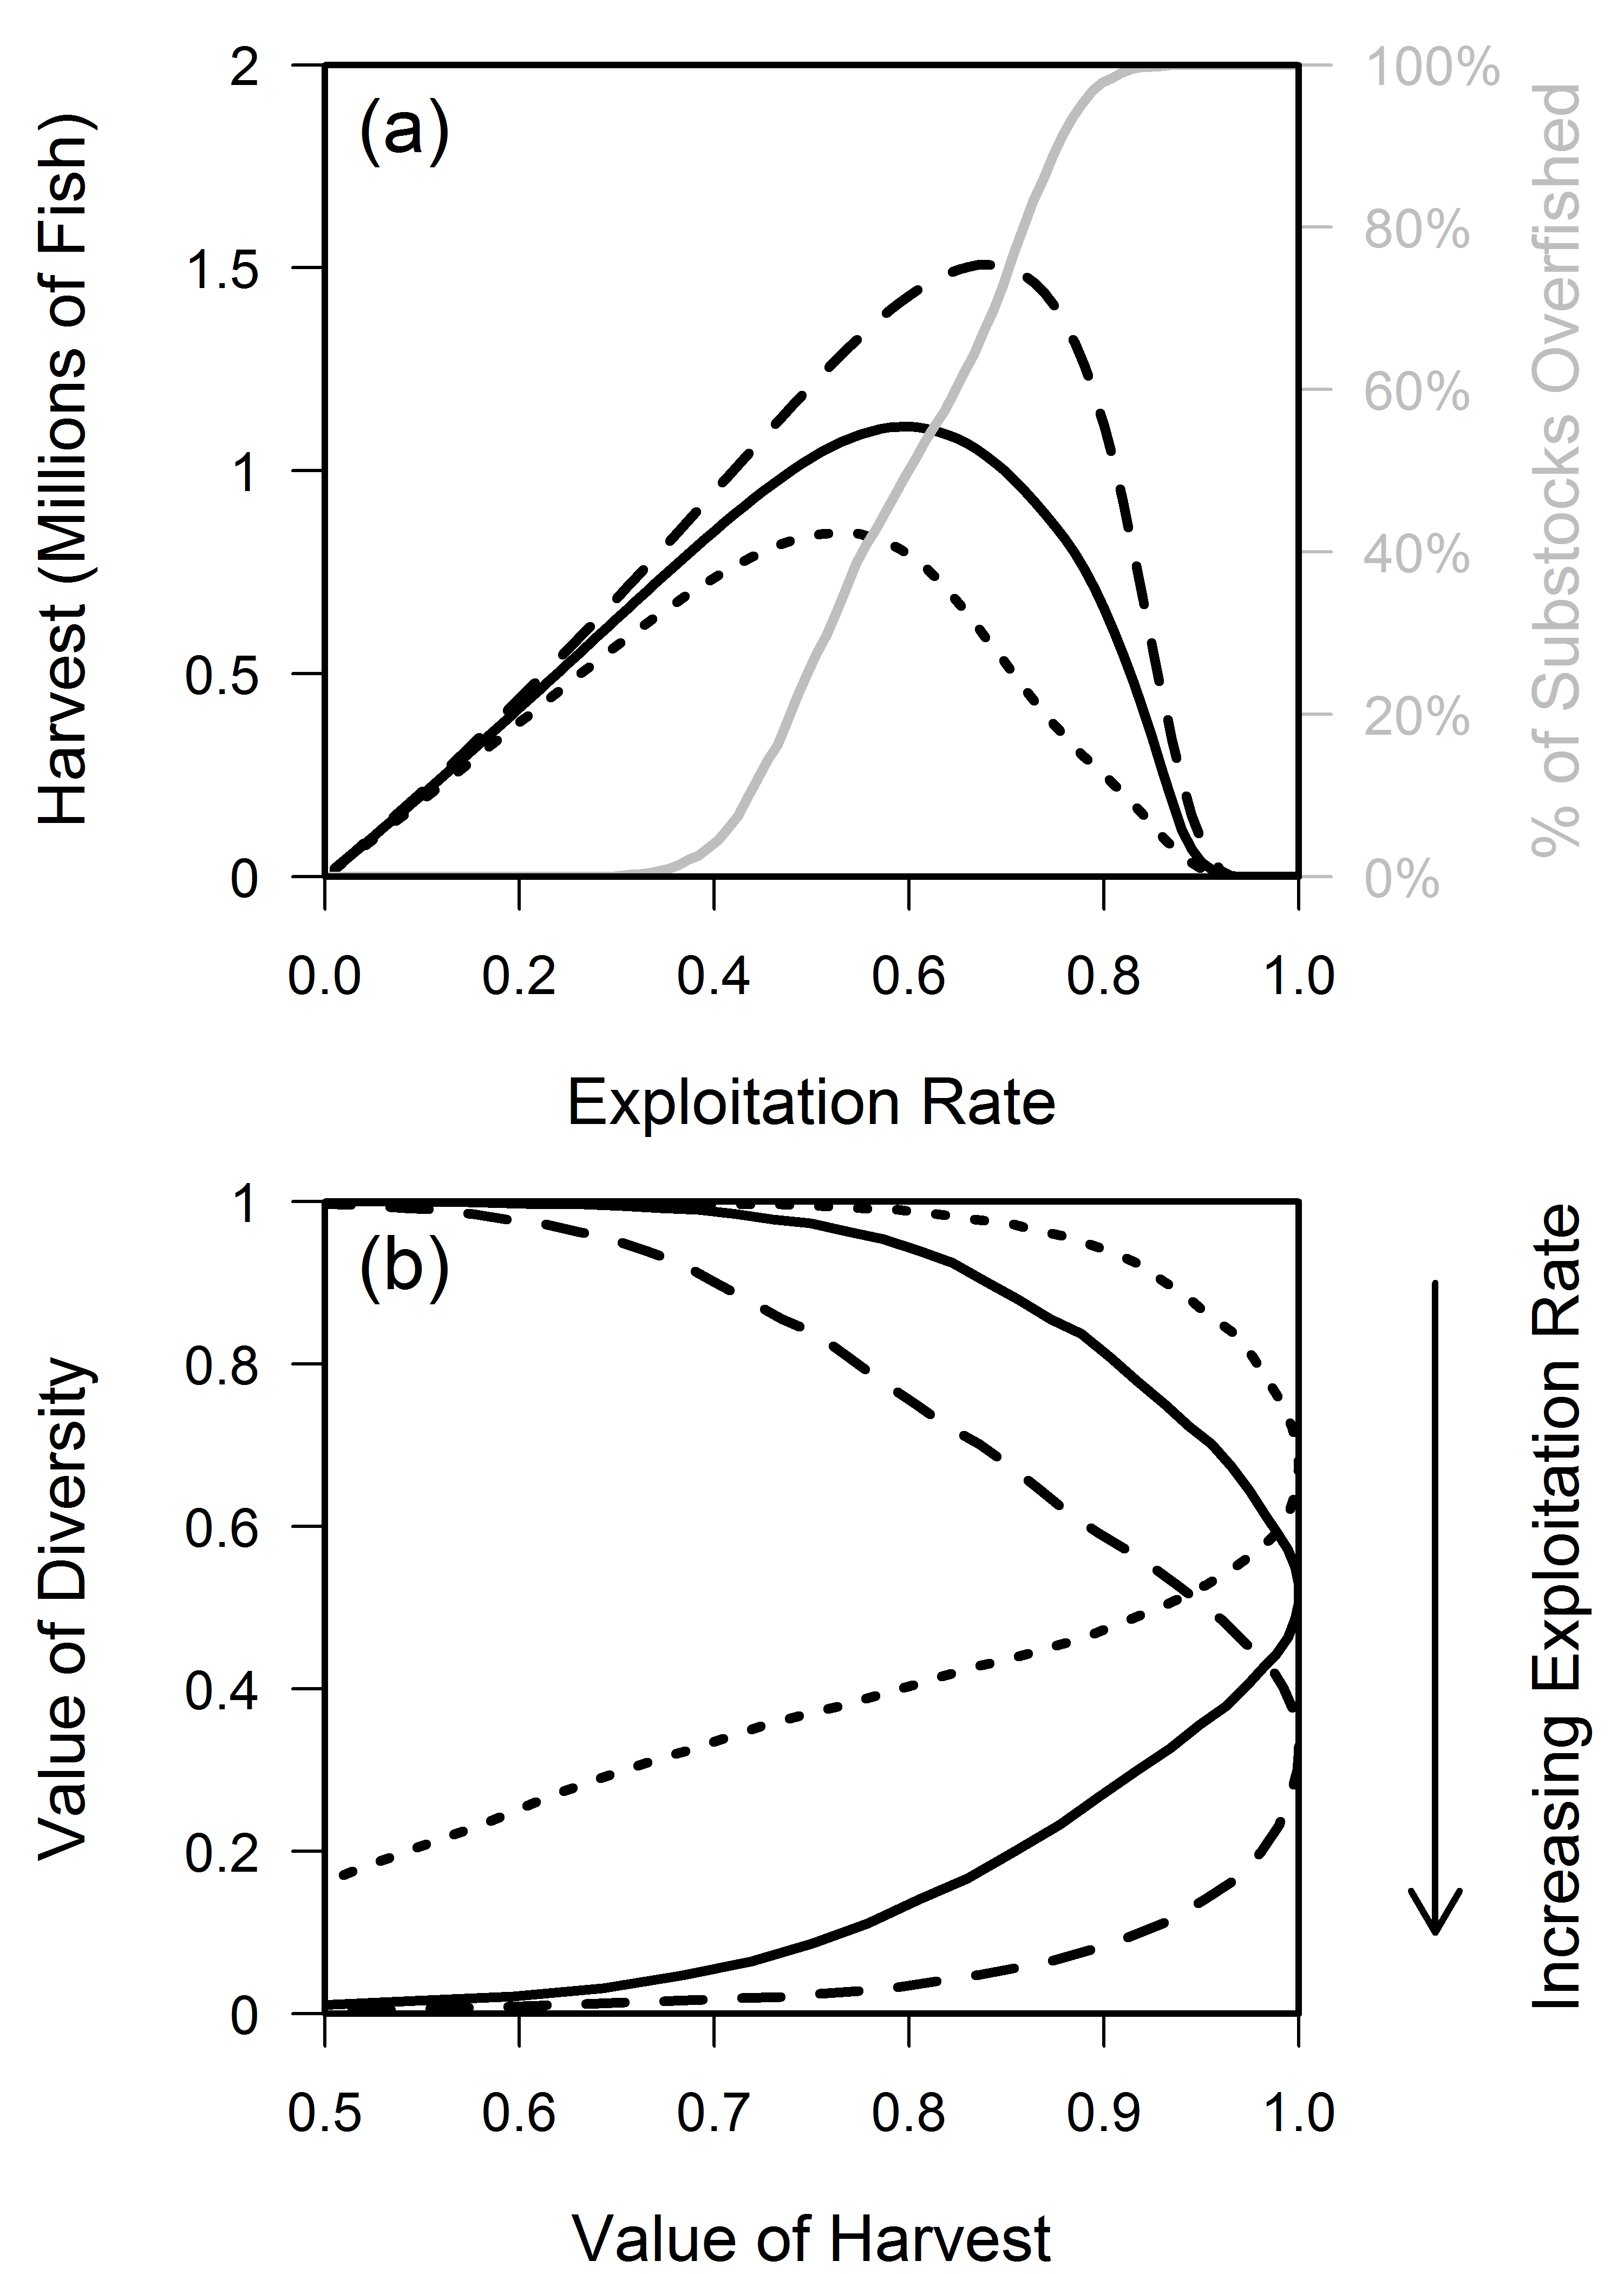
\includegraphics{img/Ch4/trade-off-plot.png}
  \caption{Visualization of how different types of heterogeneity in substock productivity and size influence the shape of trade-offs in mixed-stock salmon fisheries. Solid black likes are the case where stock types are split evenly among large/small and productive/unproductive stocks. Dotted black likes are the case where all small stocks are productive and all large stocks are unproductive, and dashed lines are the opposite (, all big stocks are productive). (\textit{a}) Equilibrium aggregate harvest and proportion of substocks overfished plotted against the exploitation rate (\textit{b}) value of the biodiversity objective (0 = all stocks overfished) plotted against the value of harvest (the long term proportion of the aggregate MSY attained). Notice that when all big stocks are productive (dashed lines), the trade-off is steeper, i.e., more harvest must be sacrificed in order to ensure a greater fraction of substocks are not overfished. }
  \label{fig:trade-off-plot}
\end{figure}

\clearpage

\begin{figure}
  \centering
  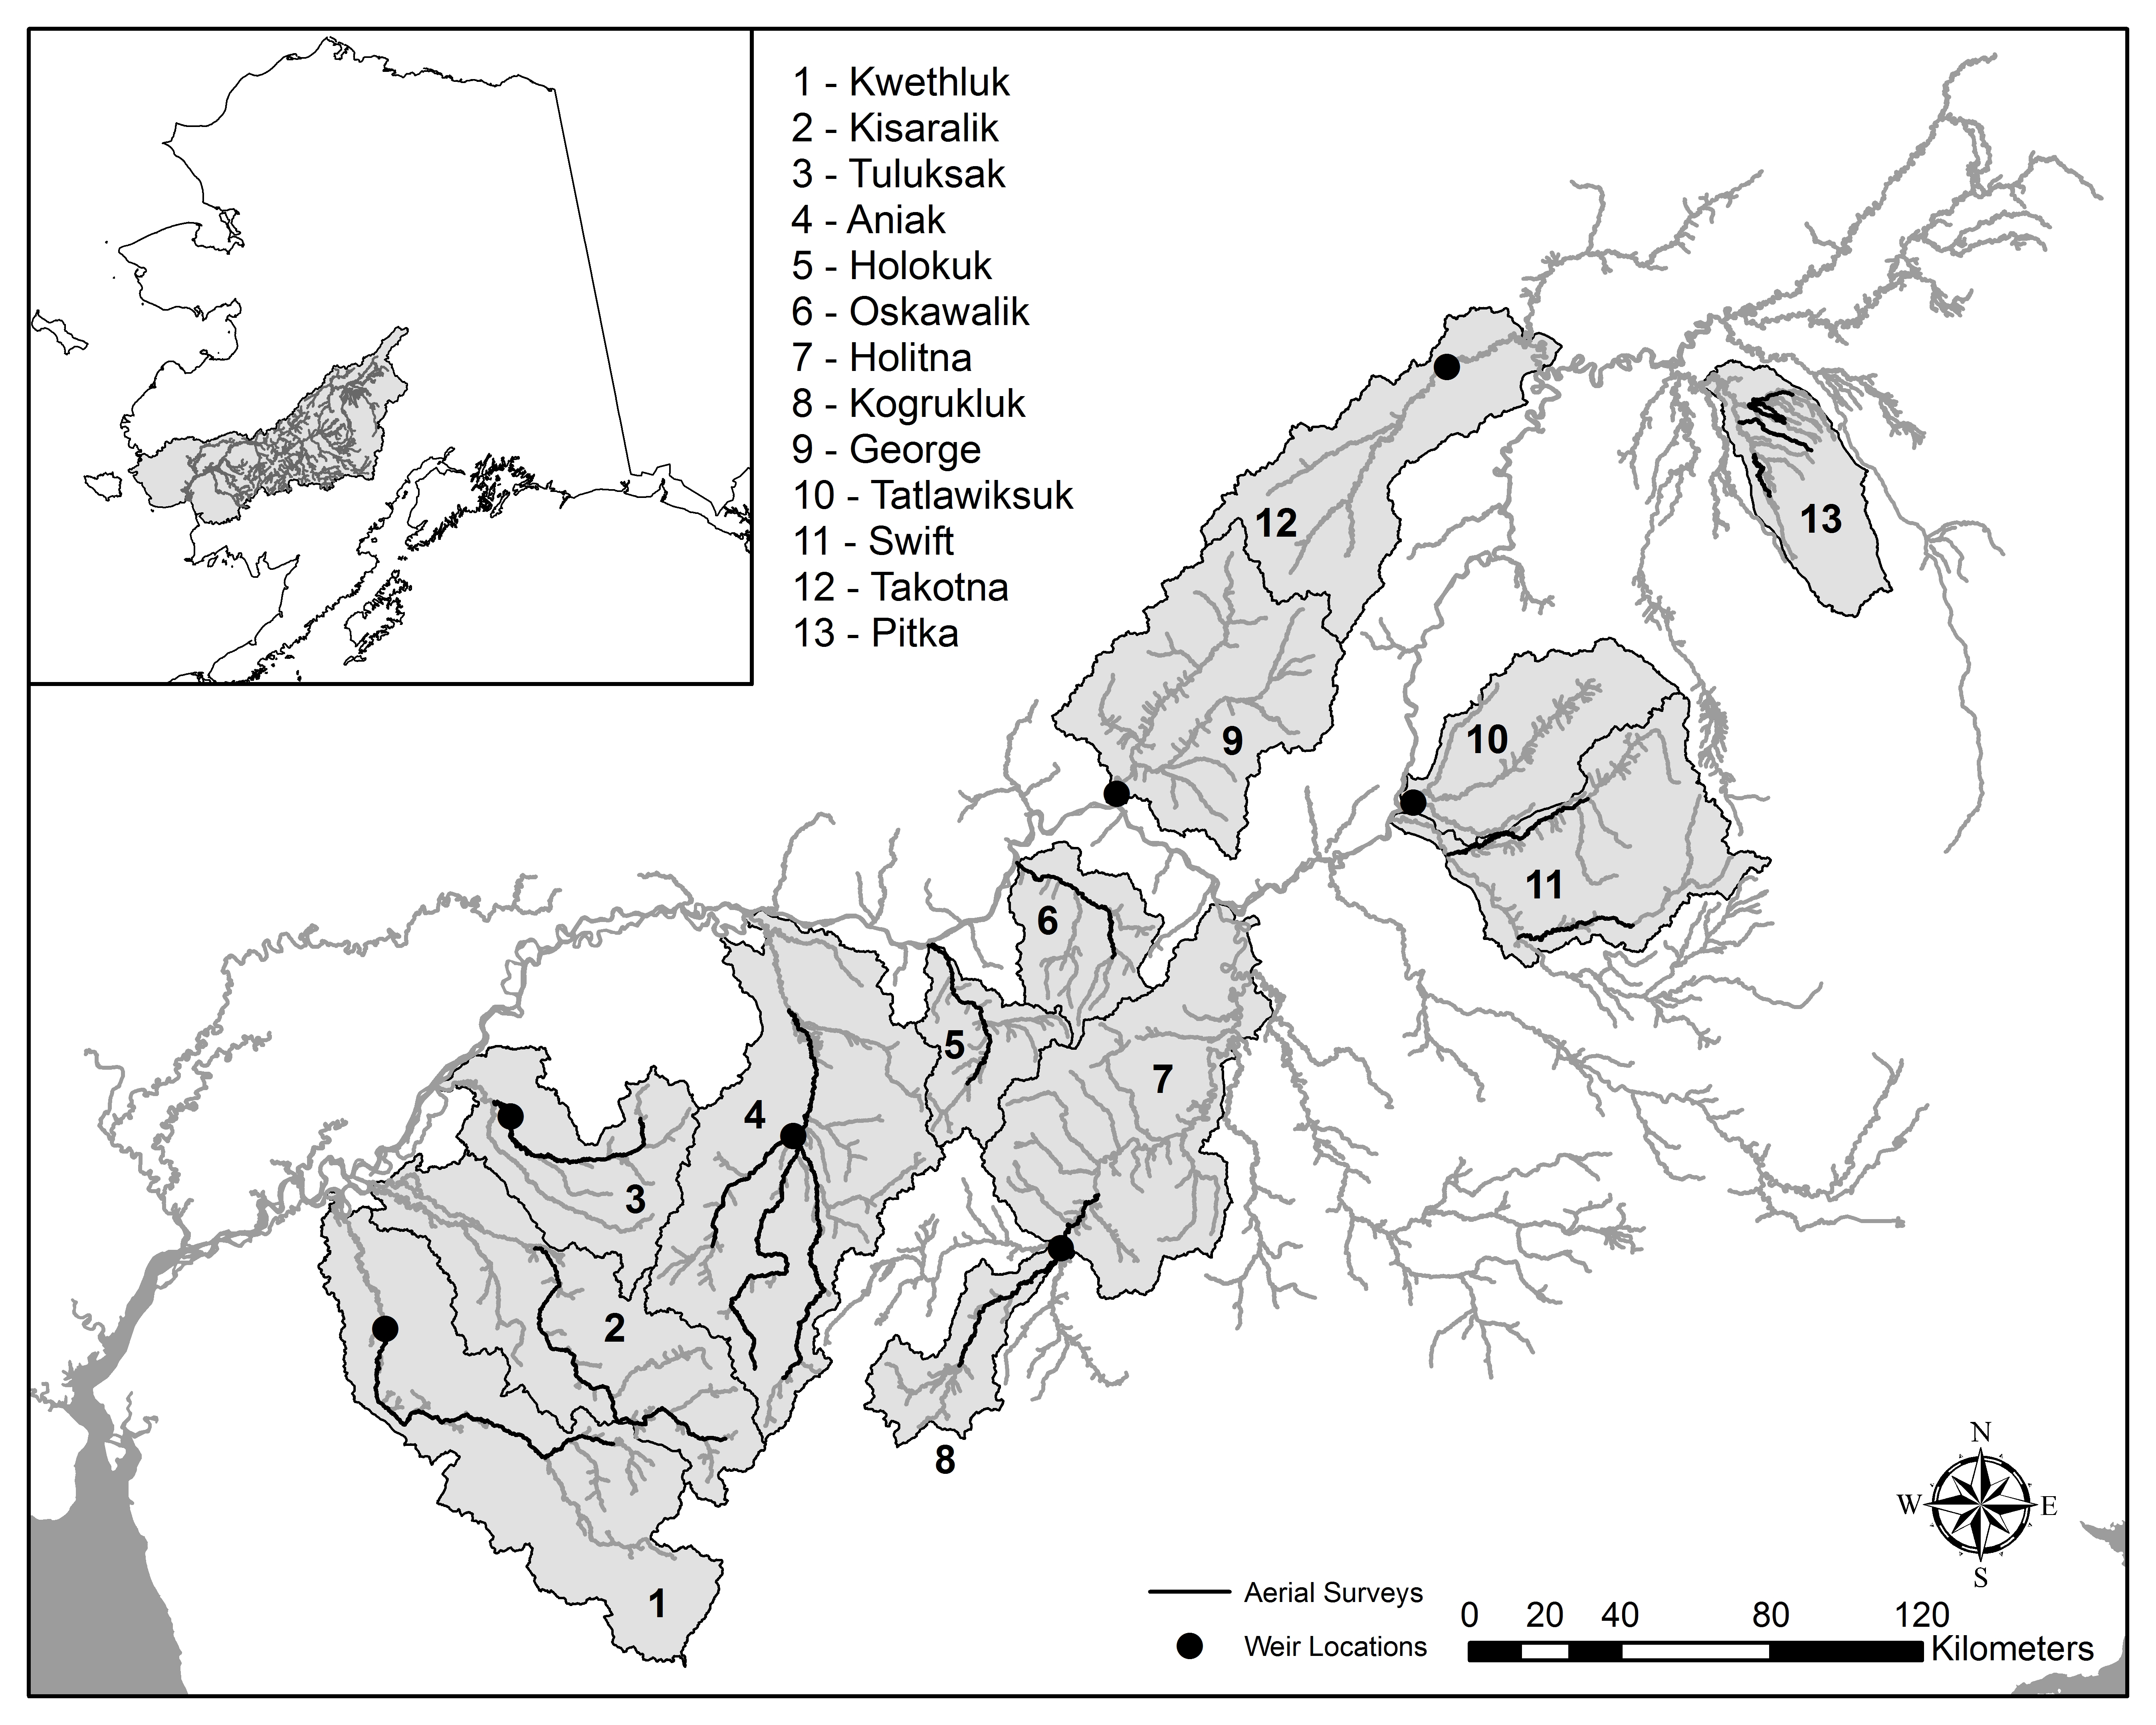
\includegraphics{img/Ch4/ch4-map.jpg}
  \caption{Map of the Kuskokwim River drainage, with the 13 drainage basins representing unique spawning units (substocks) used in this analysis. Black points show the location of weir projects, black sections of river indicate the reaches flown as part of aerial surveys. Drainages monitored via both aerial survey and weir used the weir counts to inform escapement estimates in this analysis, with the exception of the Aniak drainage (\#4), for which aerial survey data were much more abundant than the weir data.}
  \label{fig:ch4-map}
\end{figure}

\clearpage

\begin{figure}
  \centering
  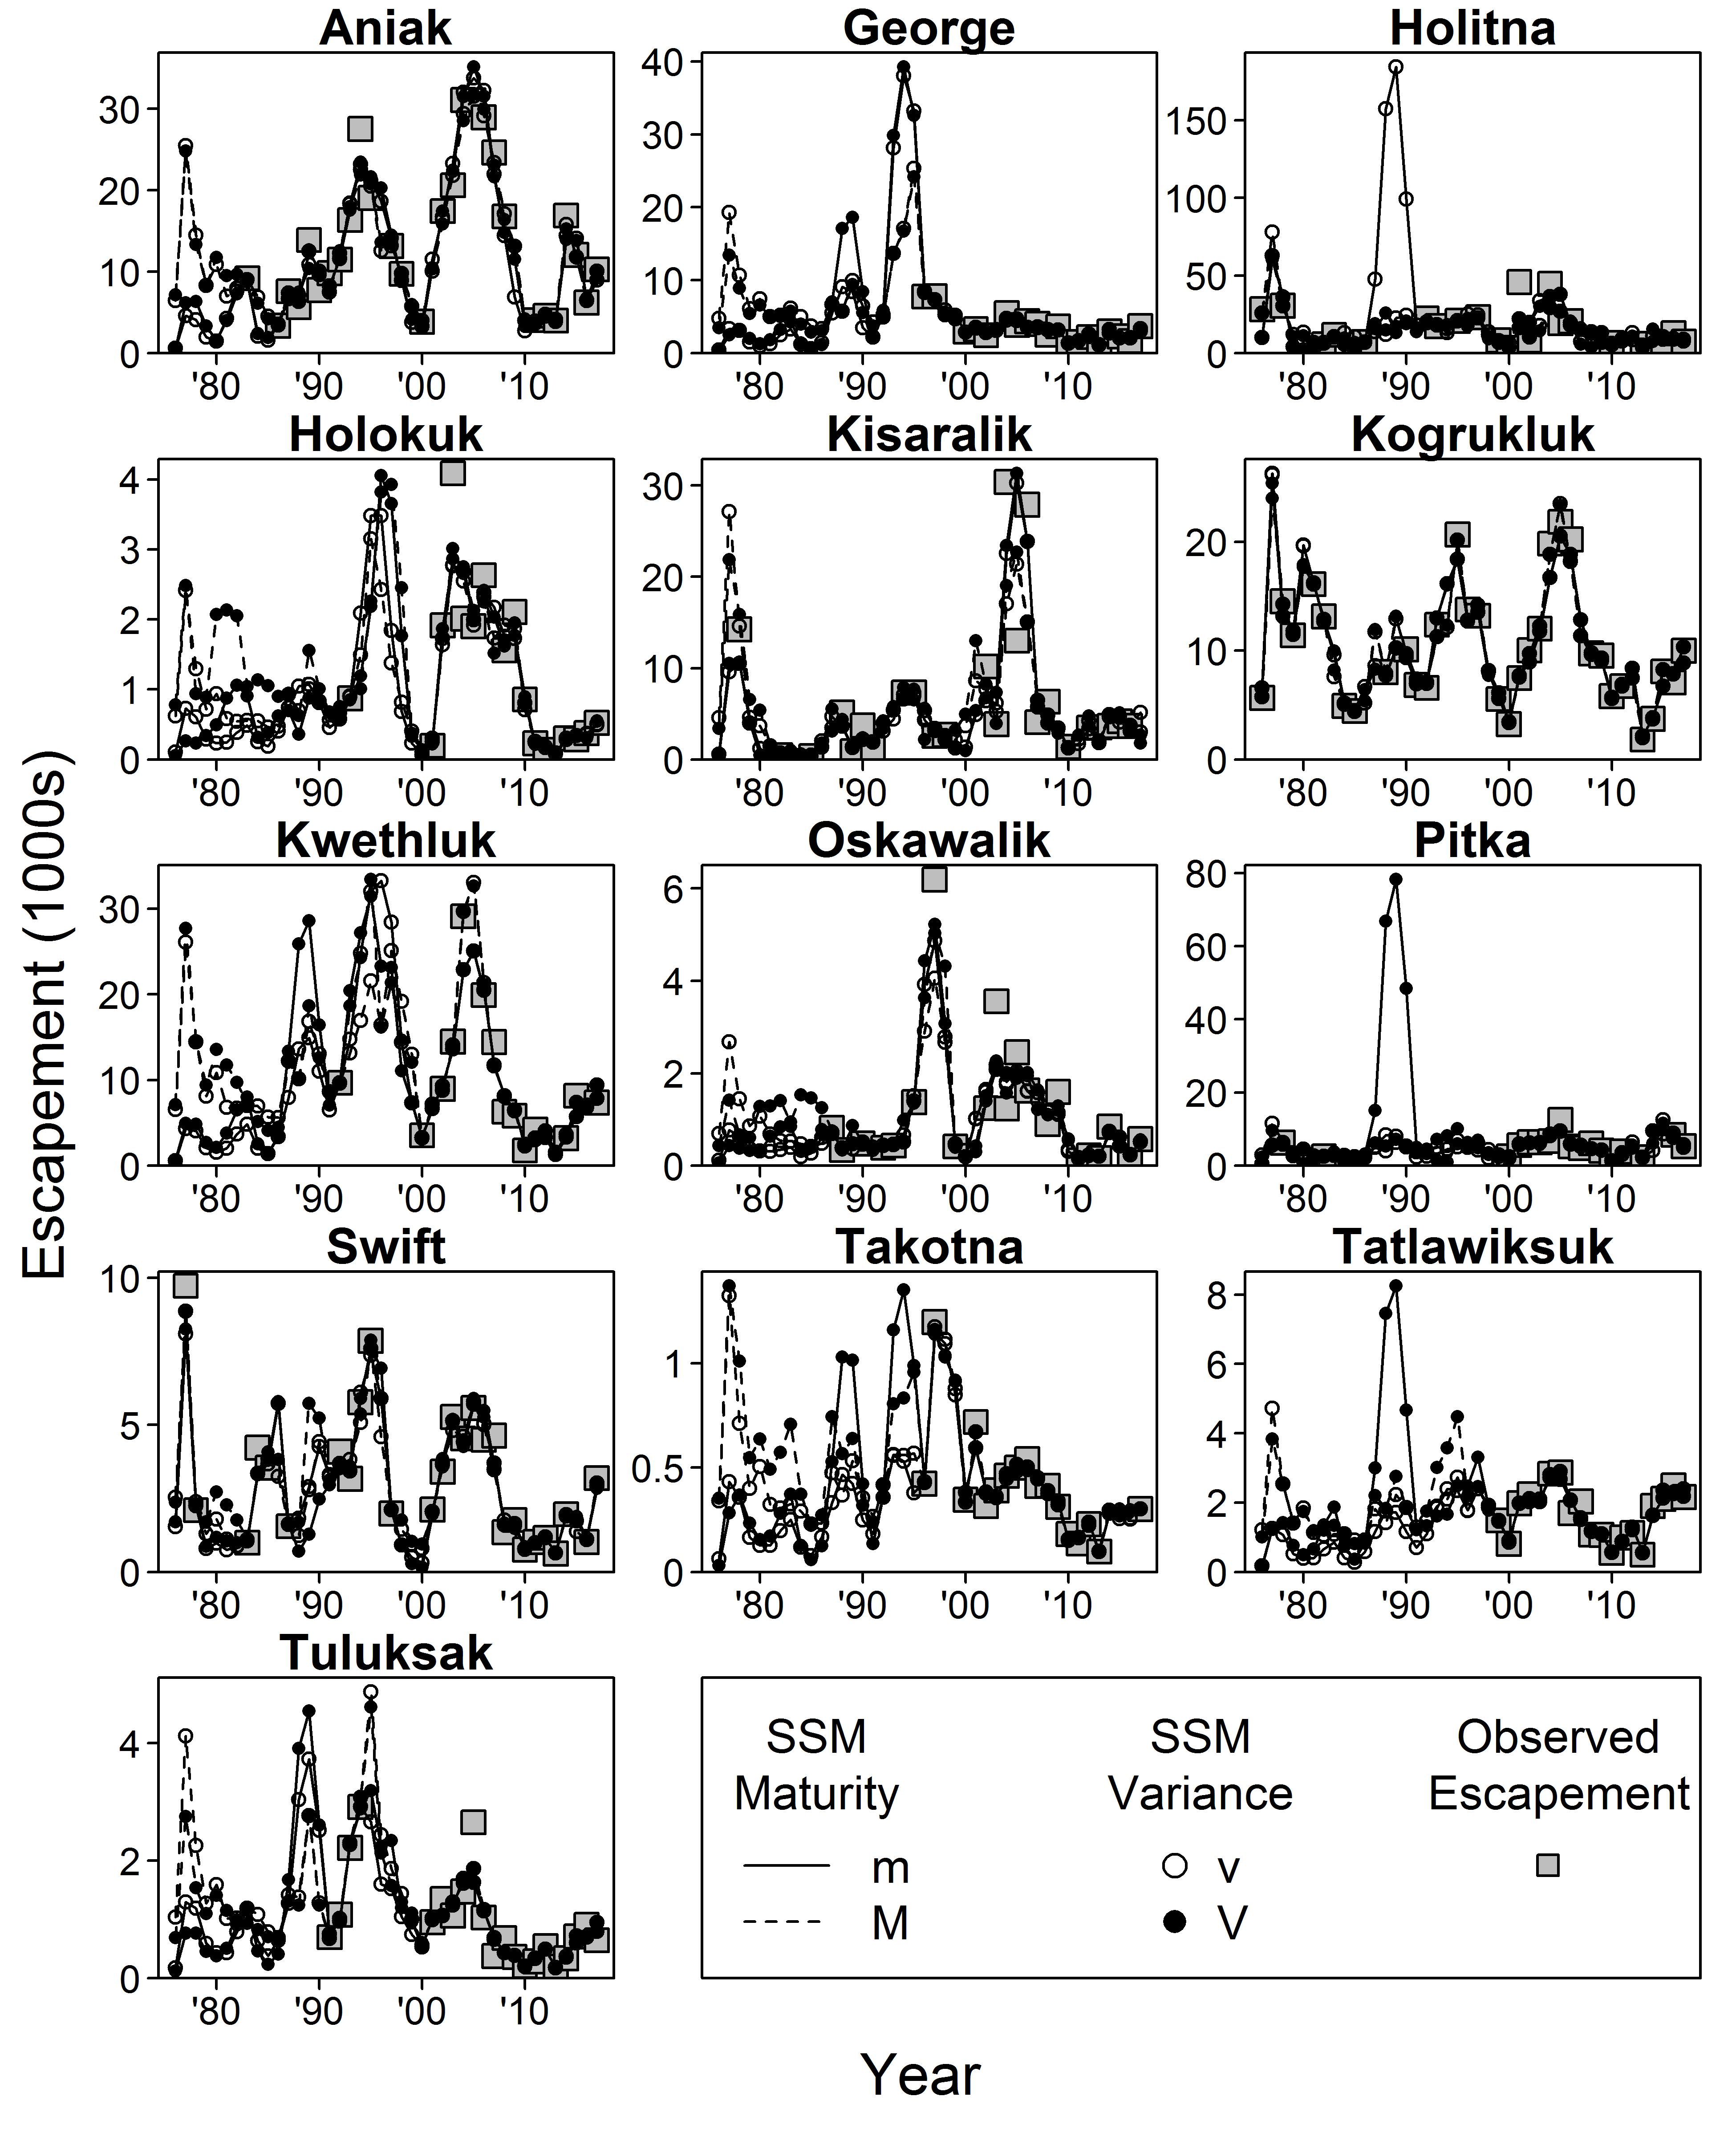
\includegraphics{img/Ch4/S-fit.jpg}
  \caption{Observed and fitted escapement time series for each Kuskokwim River substock. Line/symbol types denote the particular state-space model and grey squares denote observed data.}
  \label{fig:S-fit}
\end{figure}

\clearpage

\begin{figure}
  \centering
  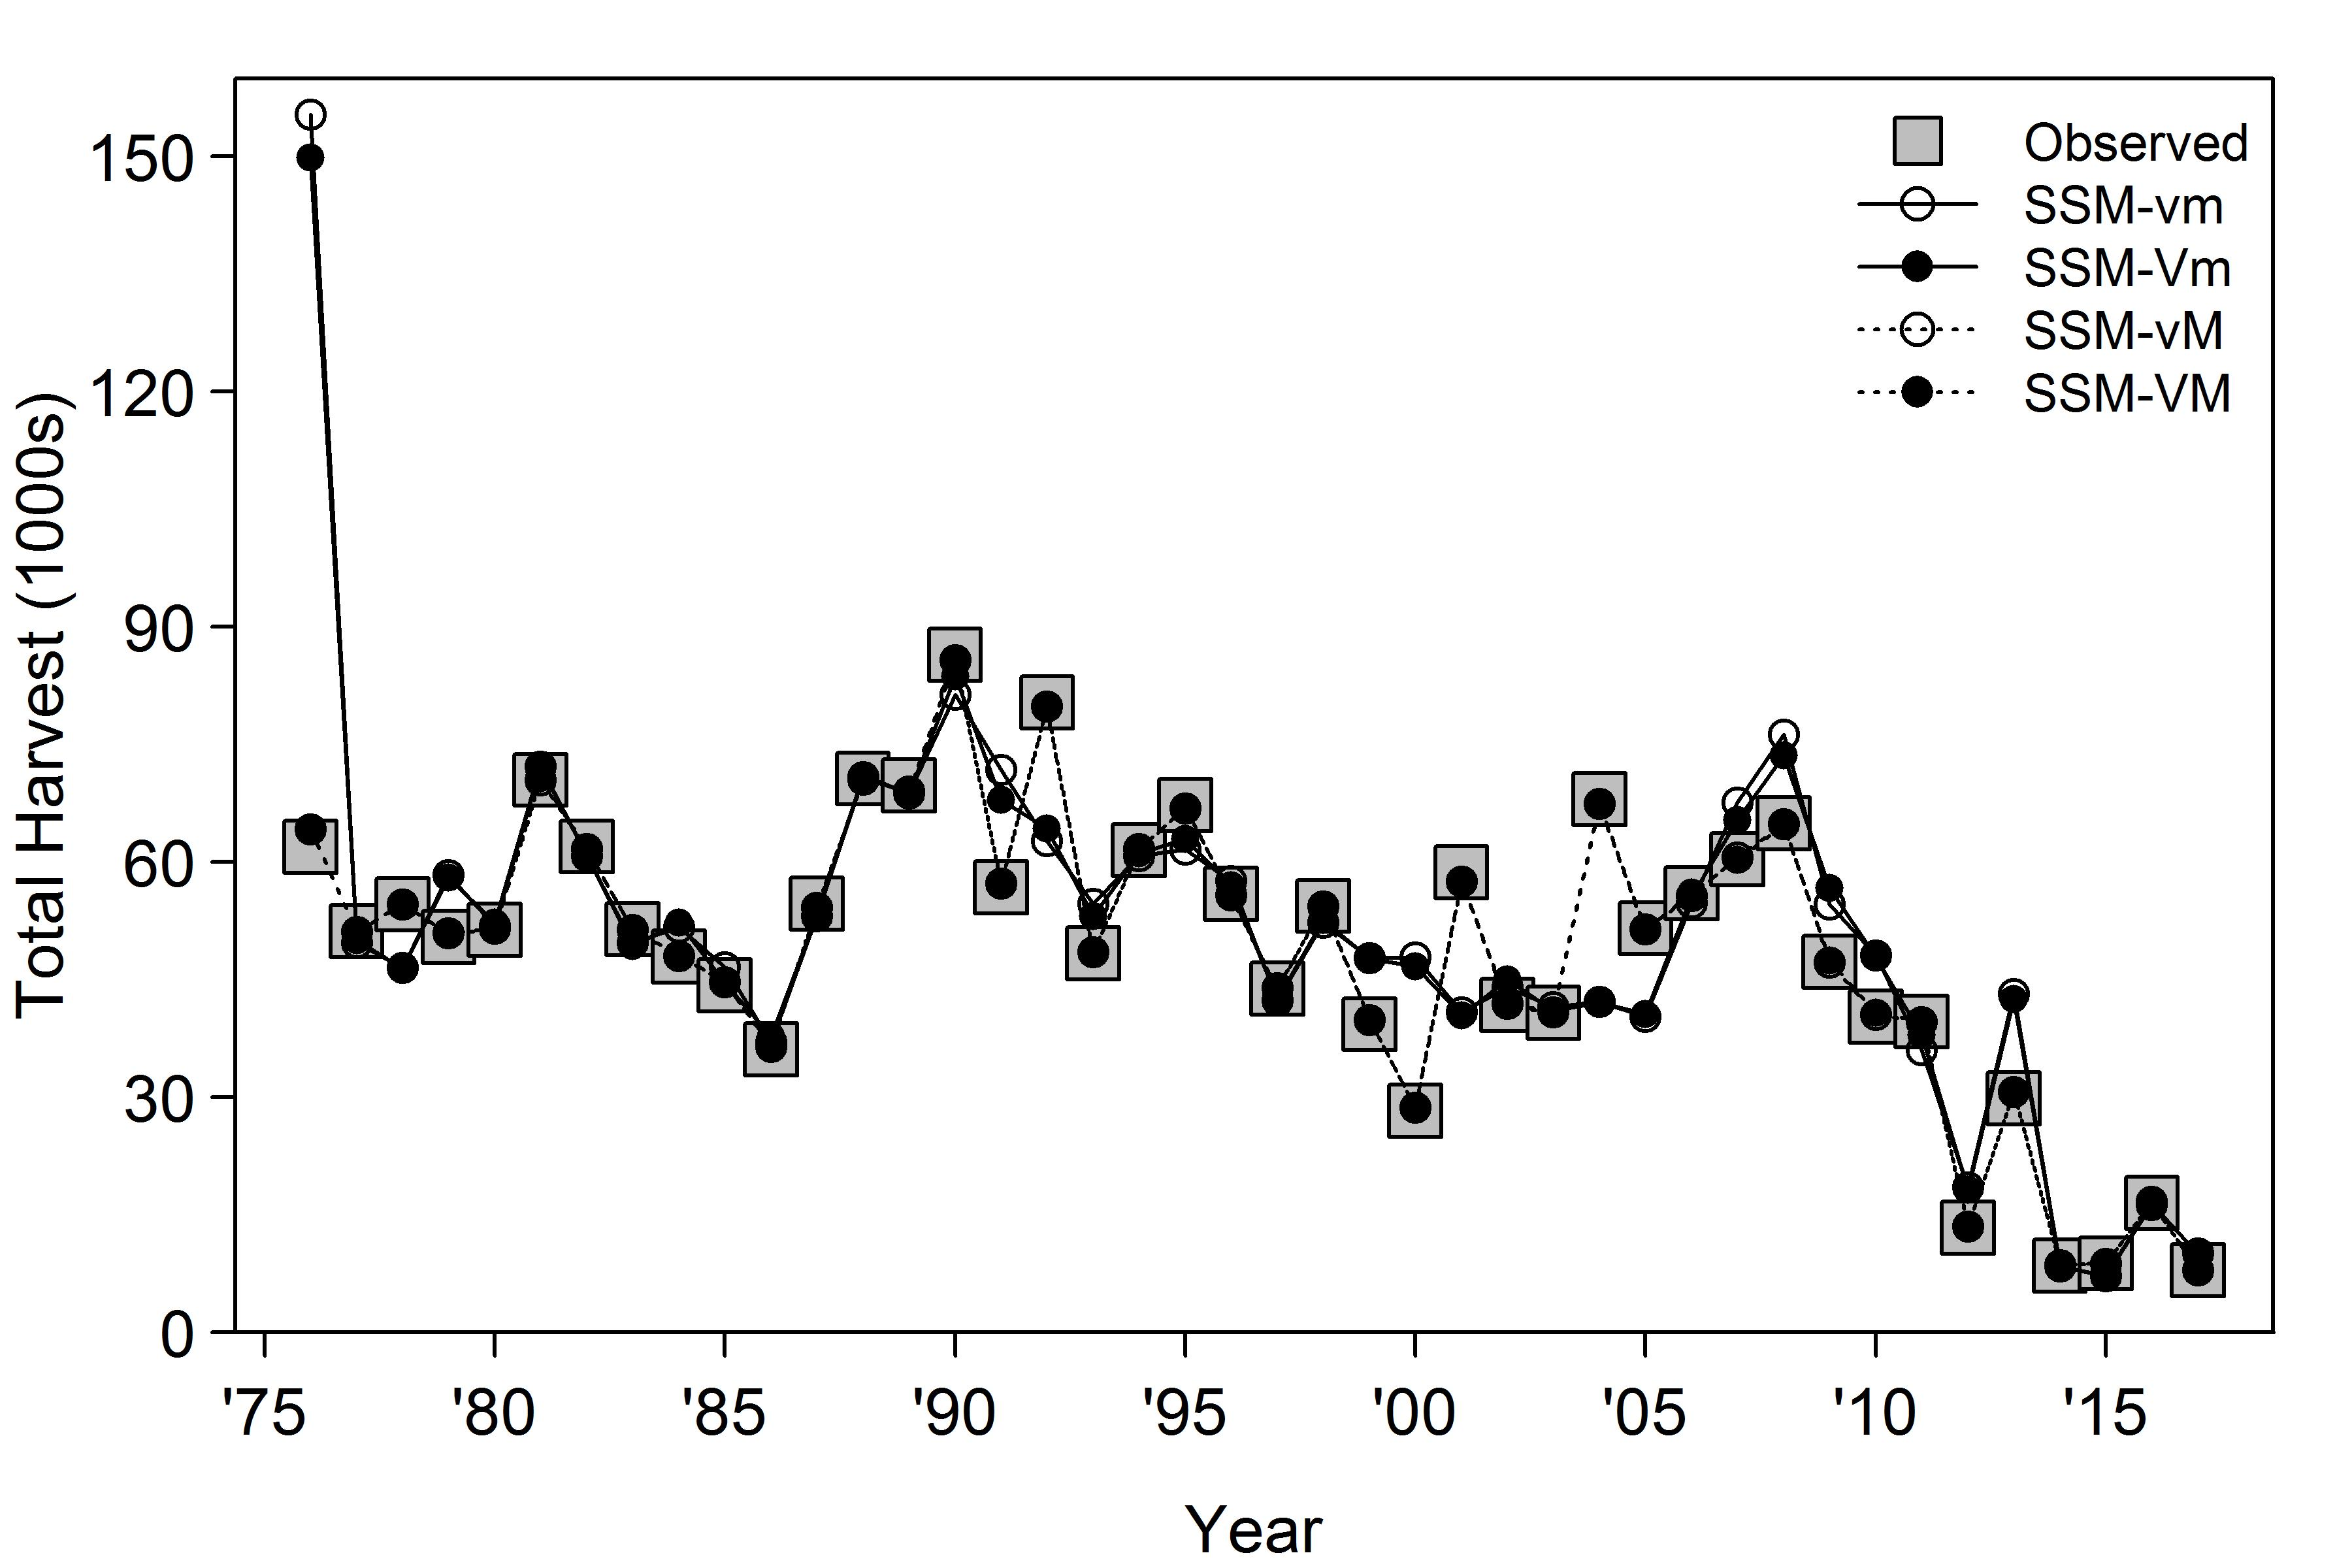
\includegraphics{img/Ch4/H-fit.jpg}
  \caption{Observed and fitted harvest time series aggregated across all Kuskokwim River substocks included in this analysis. Line/symbol types denote the particular state-space model and grey squares denote observed data.}
  \label{fig:H-fit}
\end{figure}

\clearpage

\begin{figure}
  \centering
  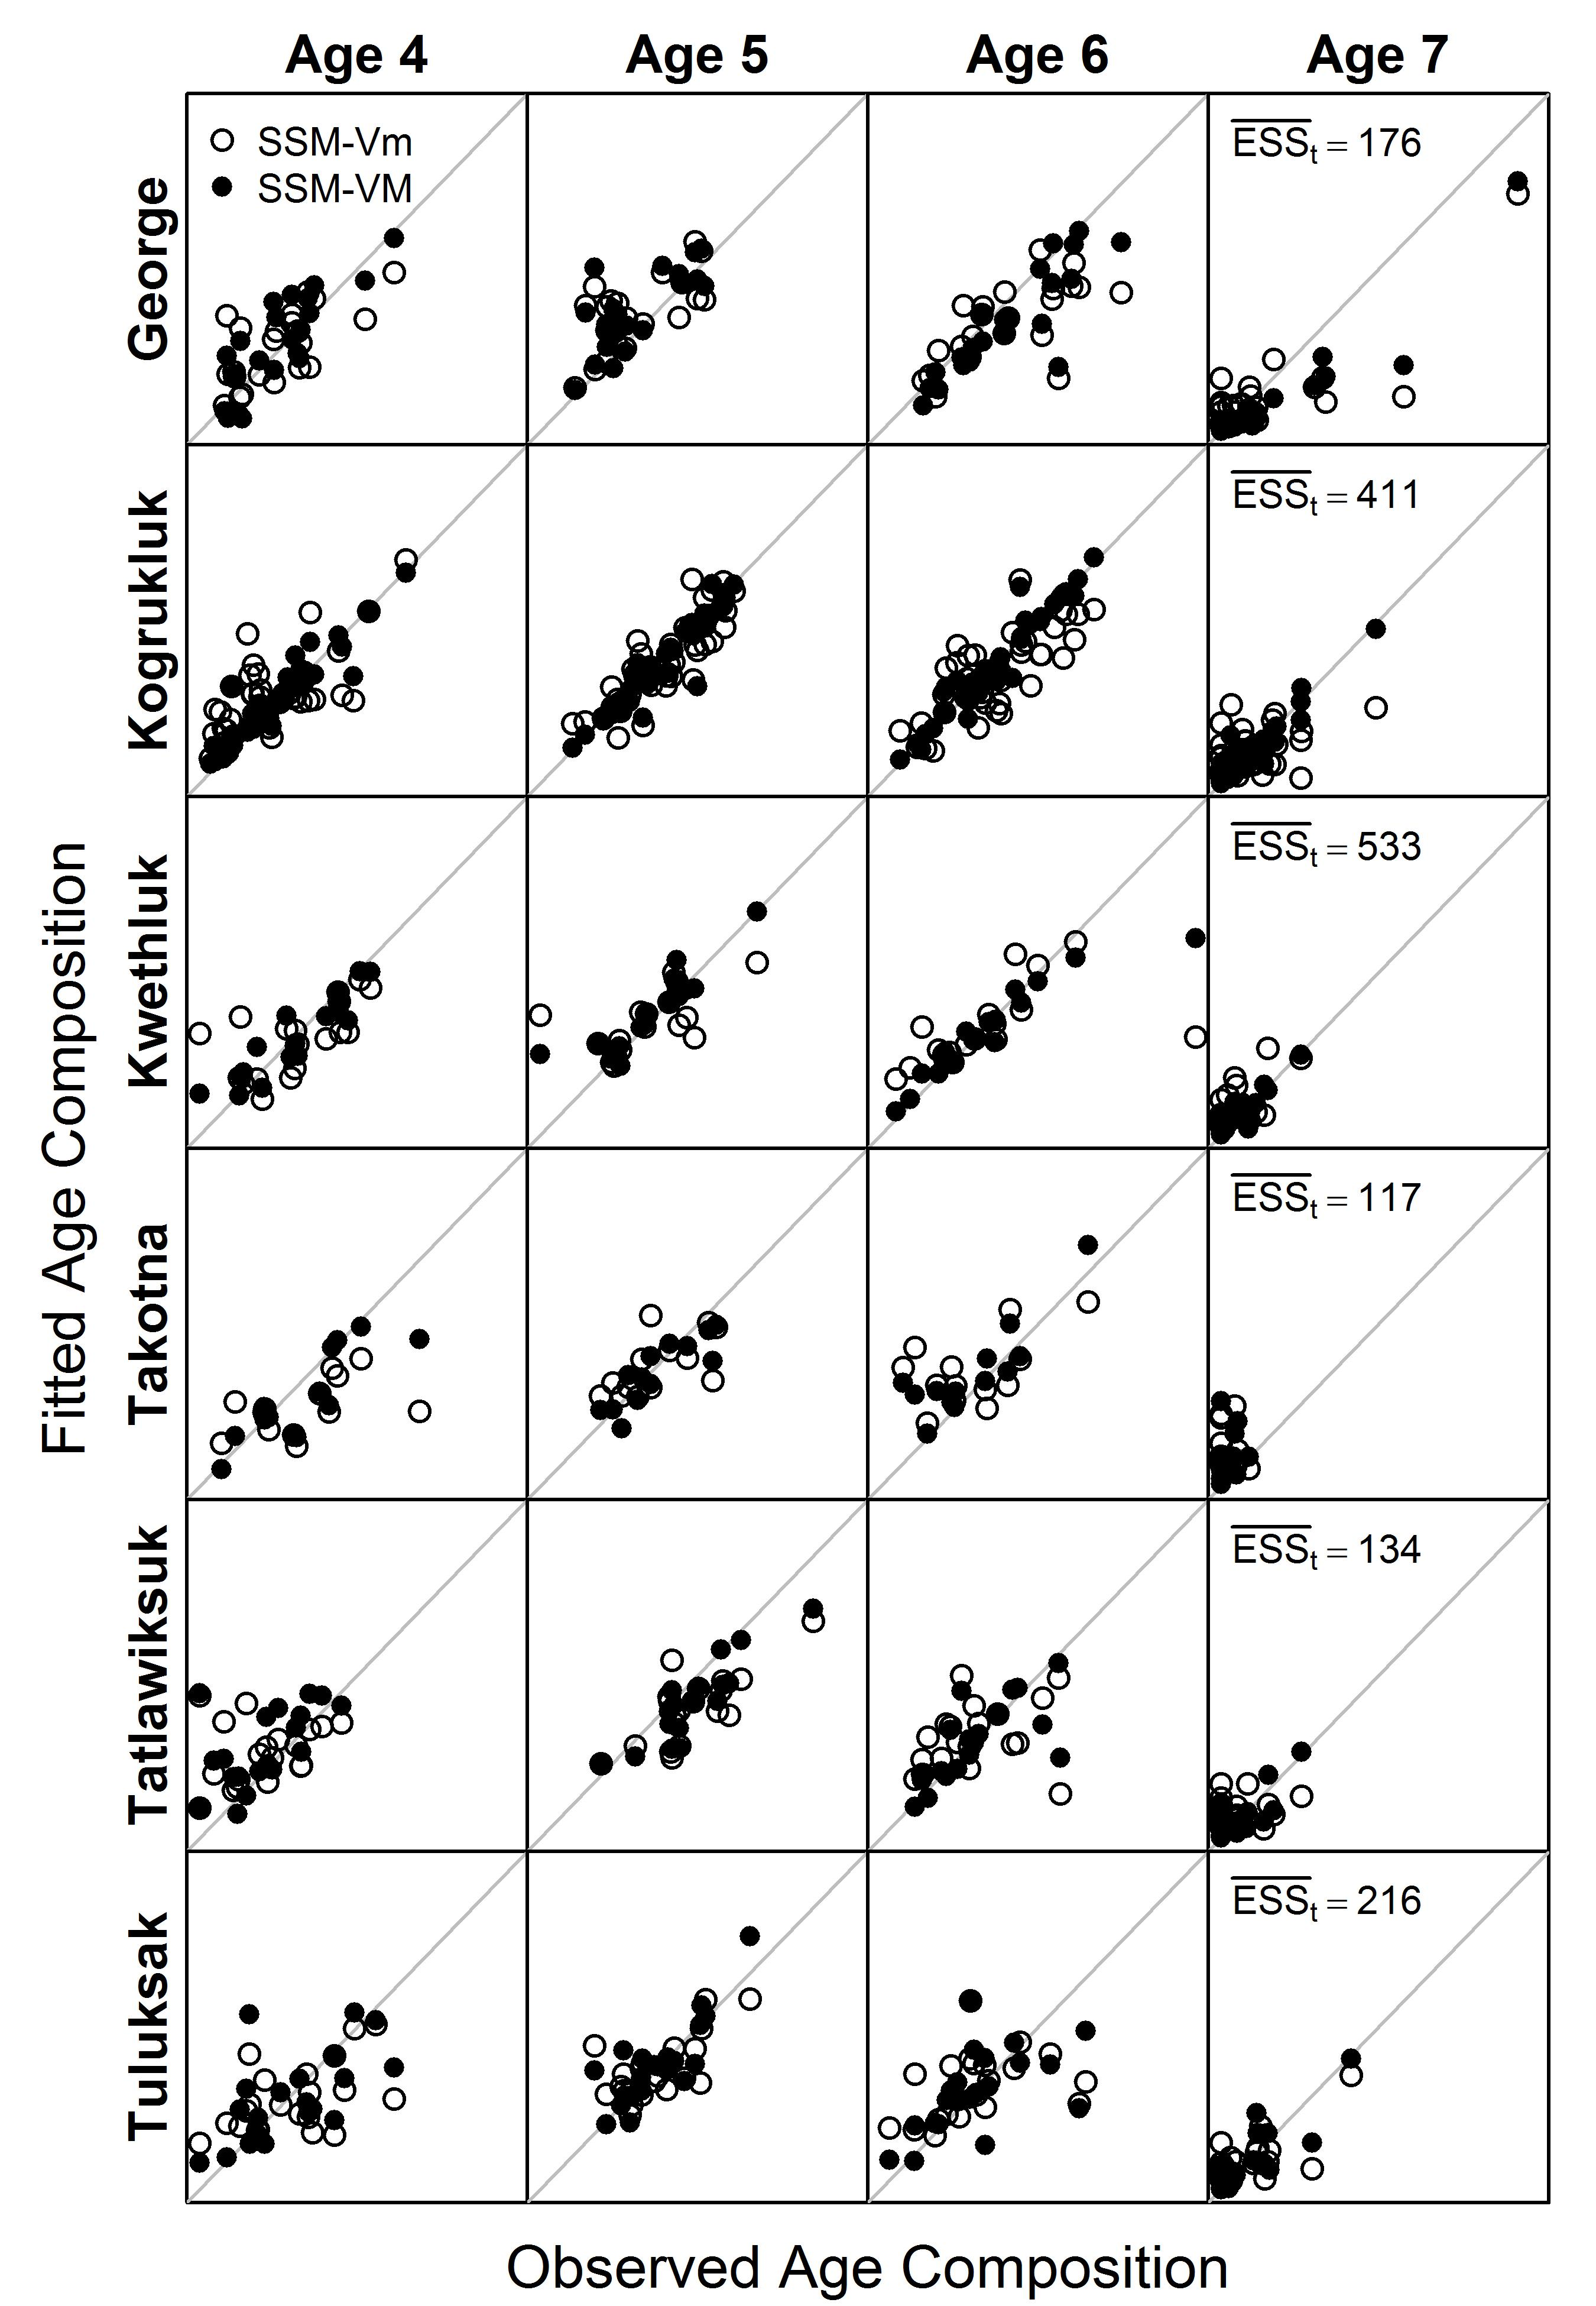
\includegraphics{img/Ch4/age-fit.jpg}
  \caption{Observed and fitted age composition for the six weir-monitored substocks. Each scatter plot is the pair of fitted \textit{versus} observed proportion of the escapement in each age each year with data available and the grey line represents the 1:1 perfect fit line. Point types denote two models: SSM-Vm (time-constant maturity; hollow circles) and SSM-VM (time-varying maturity; filled circles). $\overline{ESS}_t$ represents the average number of fish successfully aged each year with data for each substock, which was used as the sample size to weight the data in the multinomial likelihoods that used these data. Panels are scaled to have the same \textit{x}-axis and \textit{y}-axis limits within an age across substocks and range from 0 -- 1 for ages 4 -- 6 and 0 -- 0.3 for age 7.}
  \label{fig:age-fit}
\end{figure}

\clearpage

\begin{figure}
  \centering
  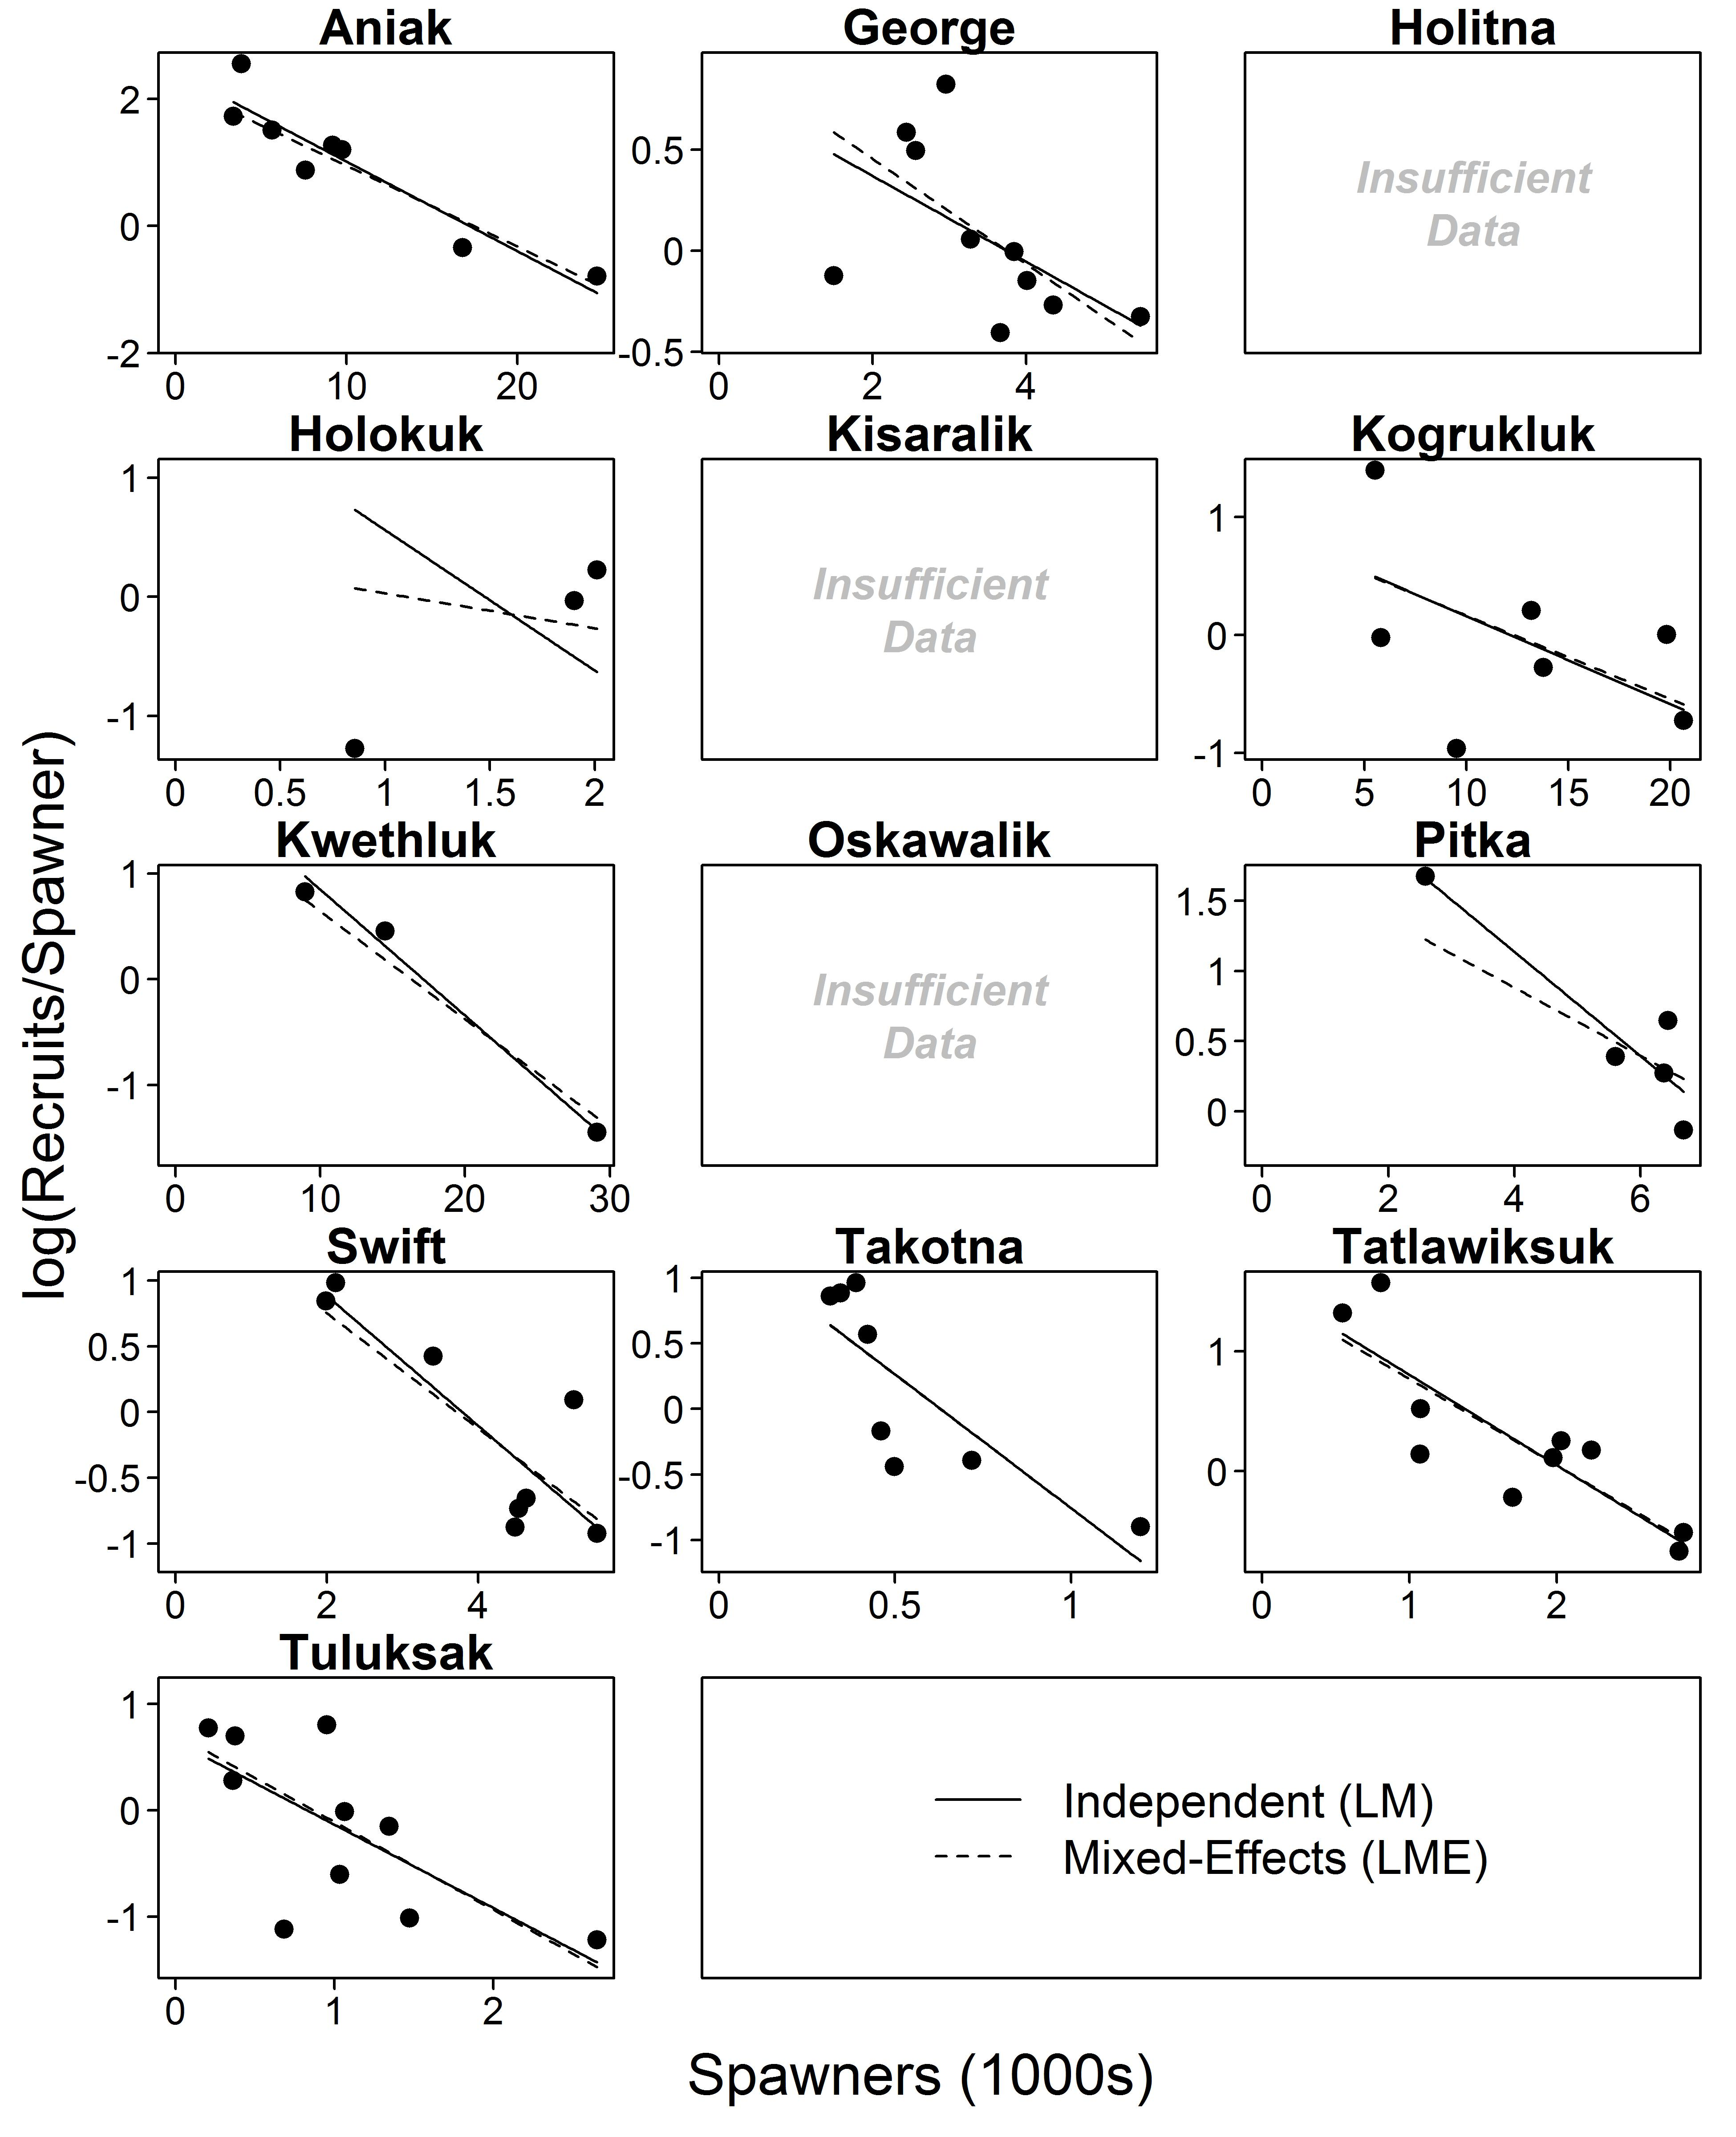
\includegraphics{img/Ch4/RPS-v-S.jpg}
  \caption{Fit of the regression approaches to fitting the multi-stock spawner-recruit analysis to the Kuskokwim River substock data. Points are observed log(recruits/spawner) \textit{versus} spawners, solid lines represent the fit for the independent regression models, and dashed lines represent the fit suggested by the model with random intercept effects for each substocks. Three substocks had fewer than three observed data points, rendering fitting a regression line infeasible. Note that a constraint was imposed that maintained $\log(\alpha_{j}) > 0$ which prevented biologically implausible values, and explains the poor fit for the Holokuk River substock.}
  \label{fig:rps-v-s}
\end{figure}

\clearpage

\begin{figure}
  \centering
  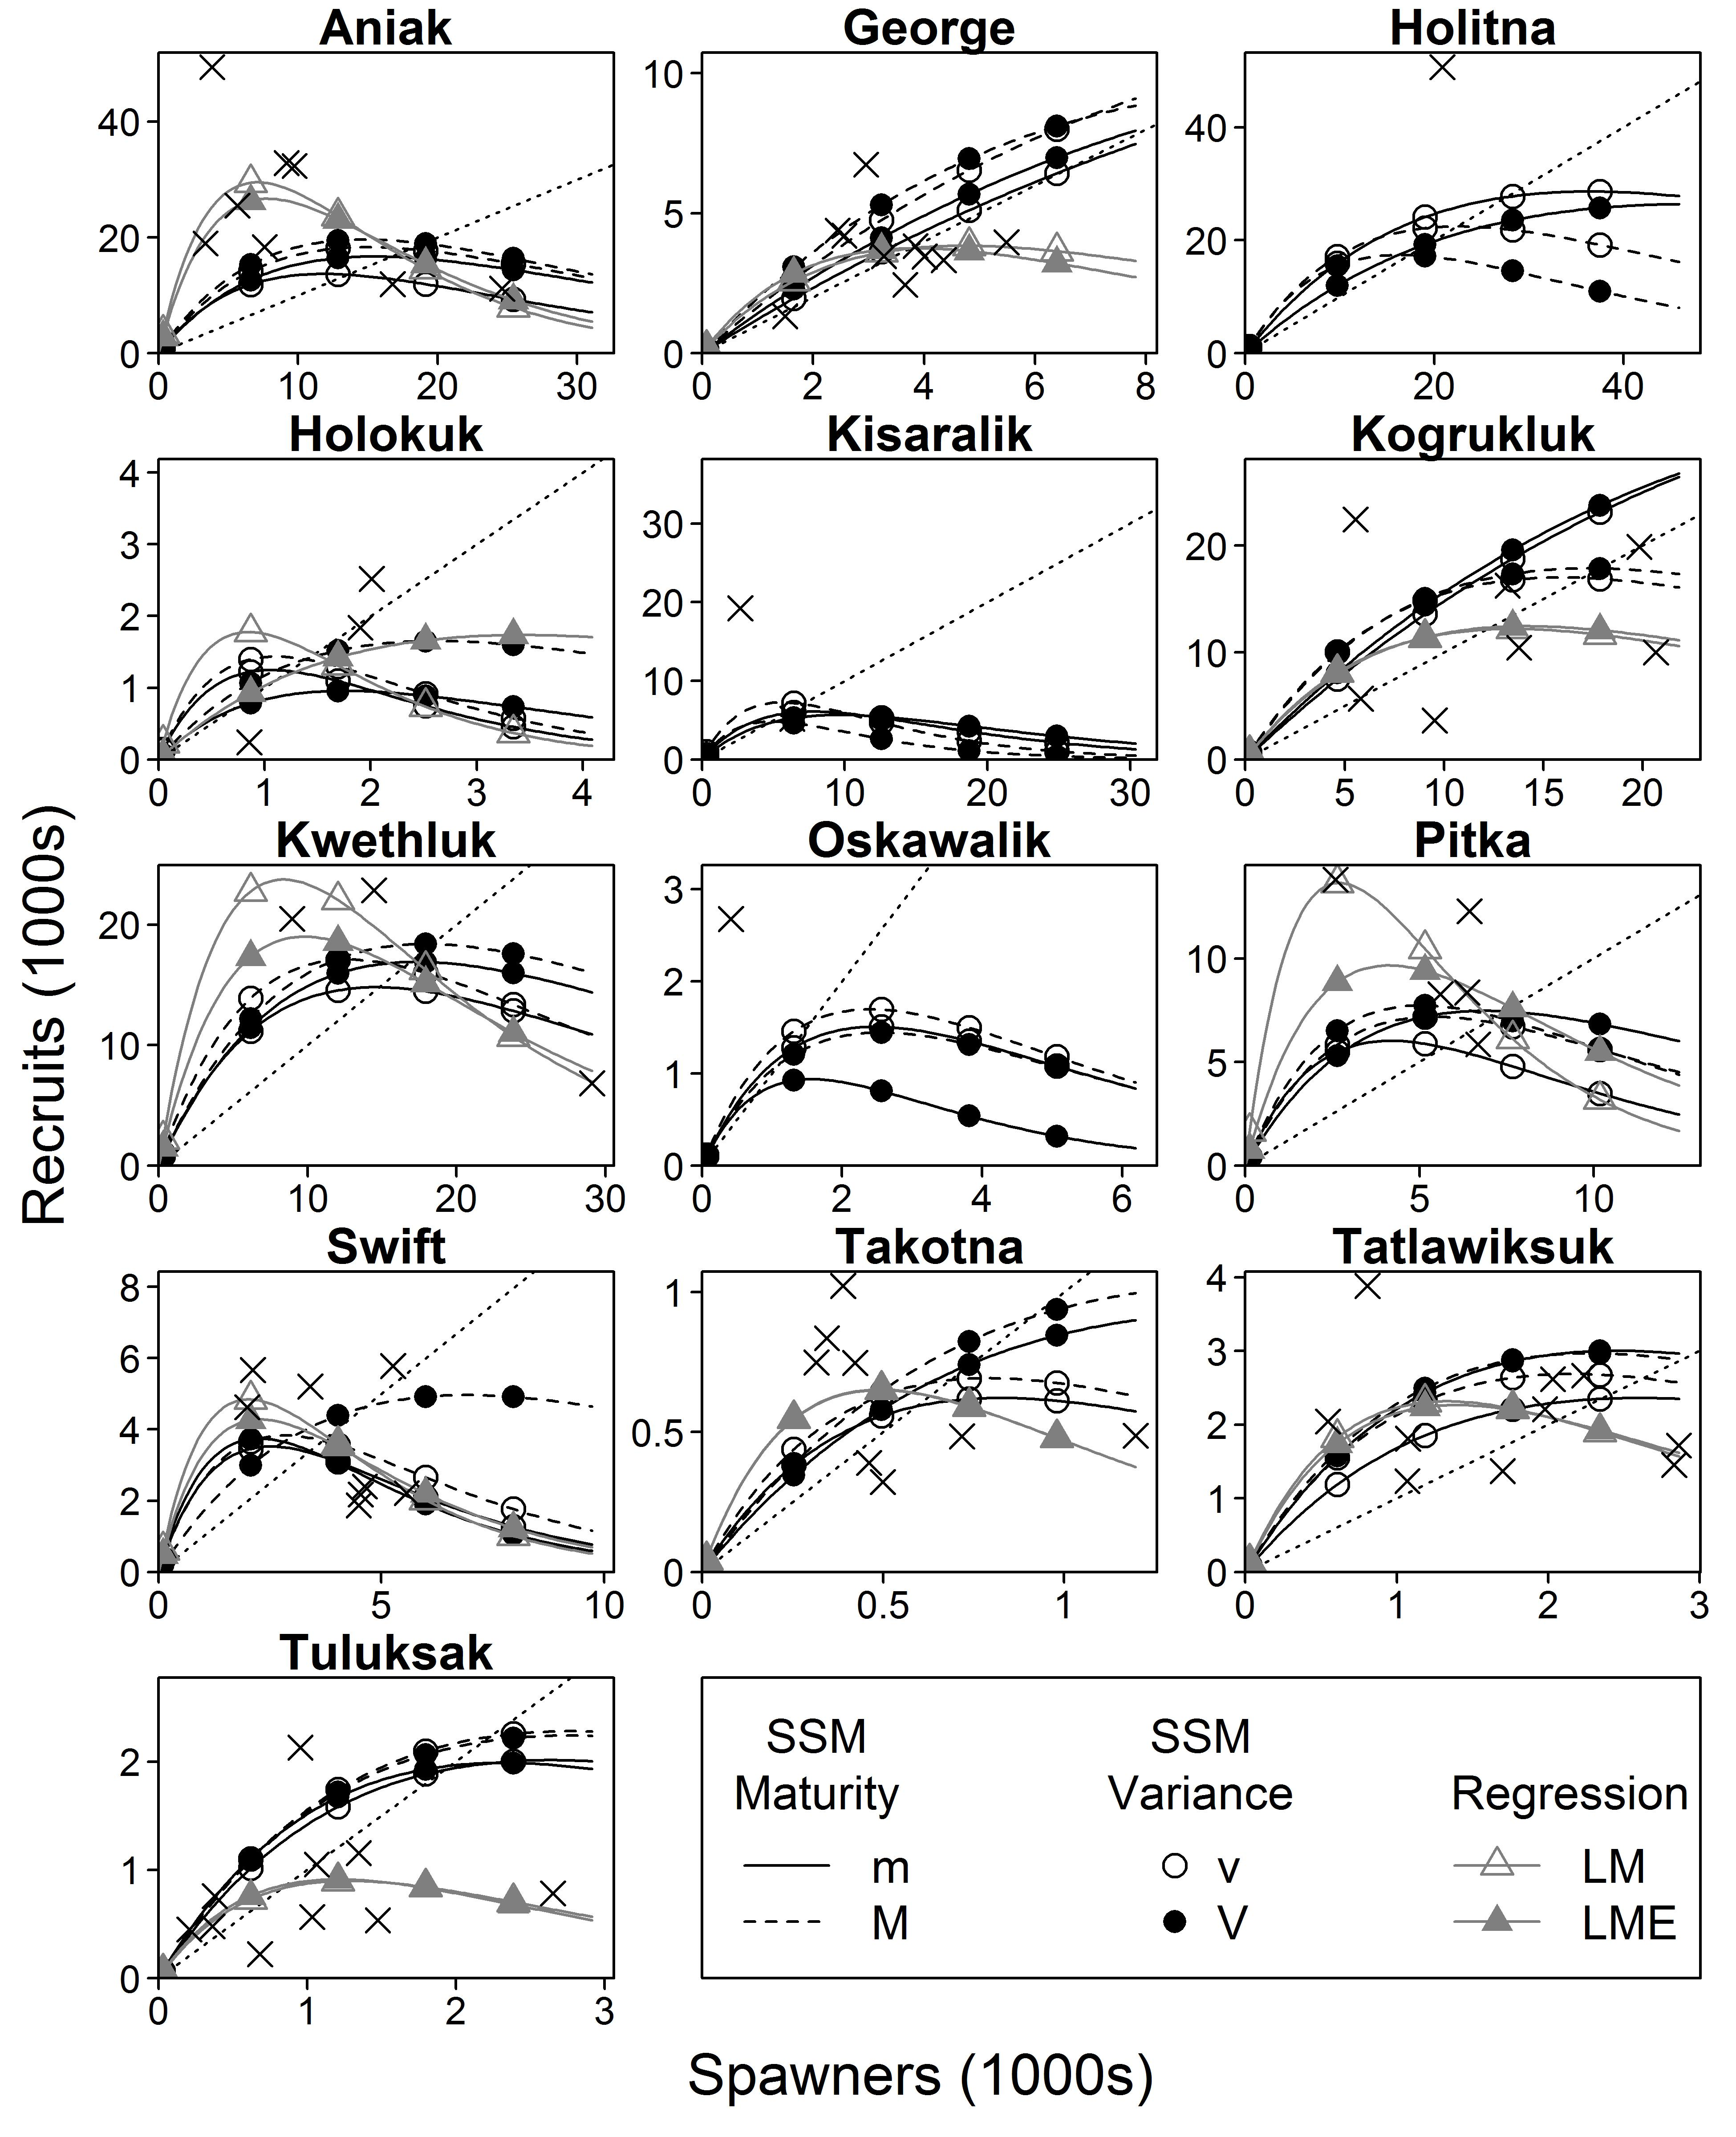
\includegraphics{img/Ch4/R-v-S.jpg}
  \caption{Fitted spawner-recruit relationships for the 13 substocks monitored in the Kuskokwim River subdrainage included in this analysis. Line and point types correspond to different models; crosses are completely-observed spawner-recruit pairs. Note that the regression approaches (grey lines/triangles) fitted only to these data, the state-space models (black lines/circles) fitted to all observations of substock-specific escapement, aggregate harvest, and age composition.}
  \label{fig:r-v-s}
\end{figure}

\clearpage

\begin{figure}
  \centering
  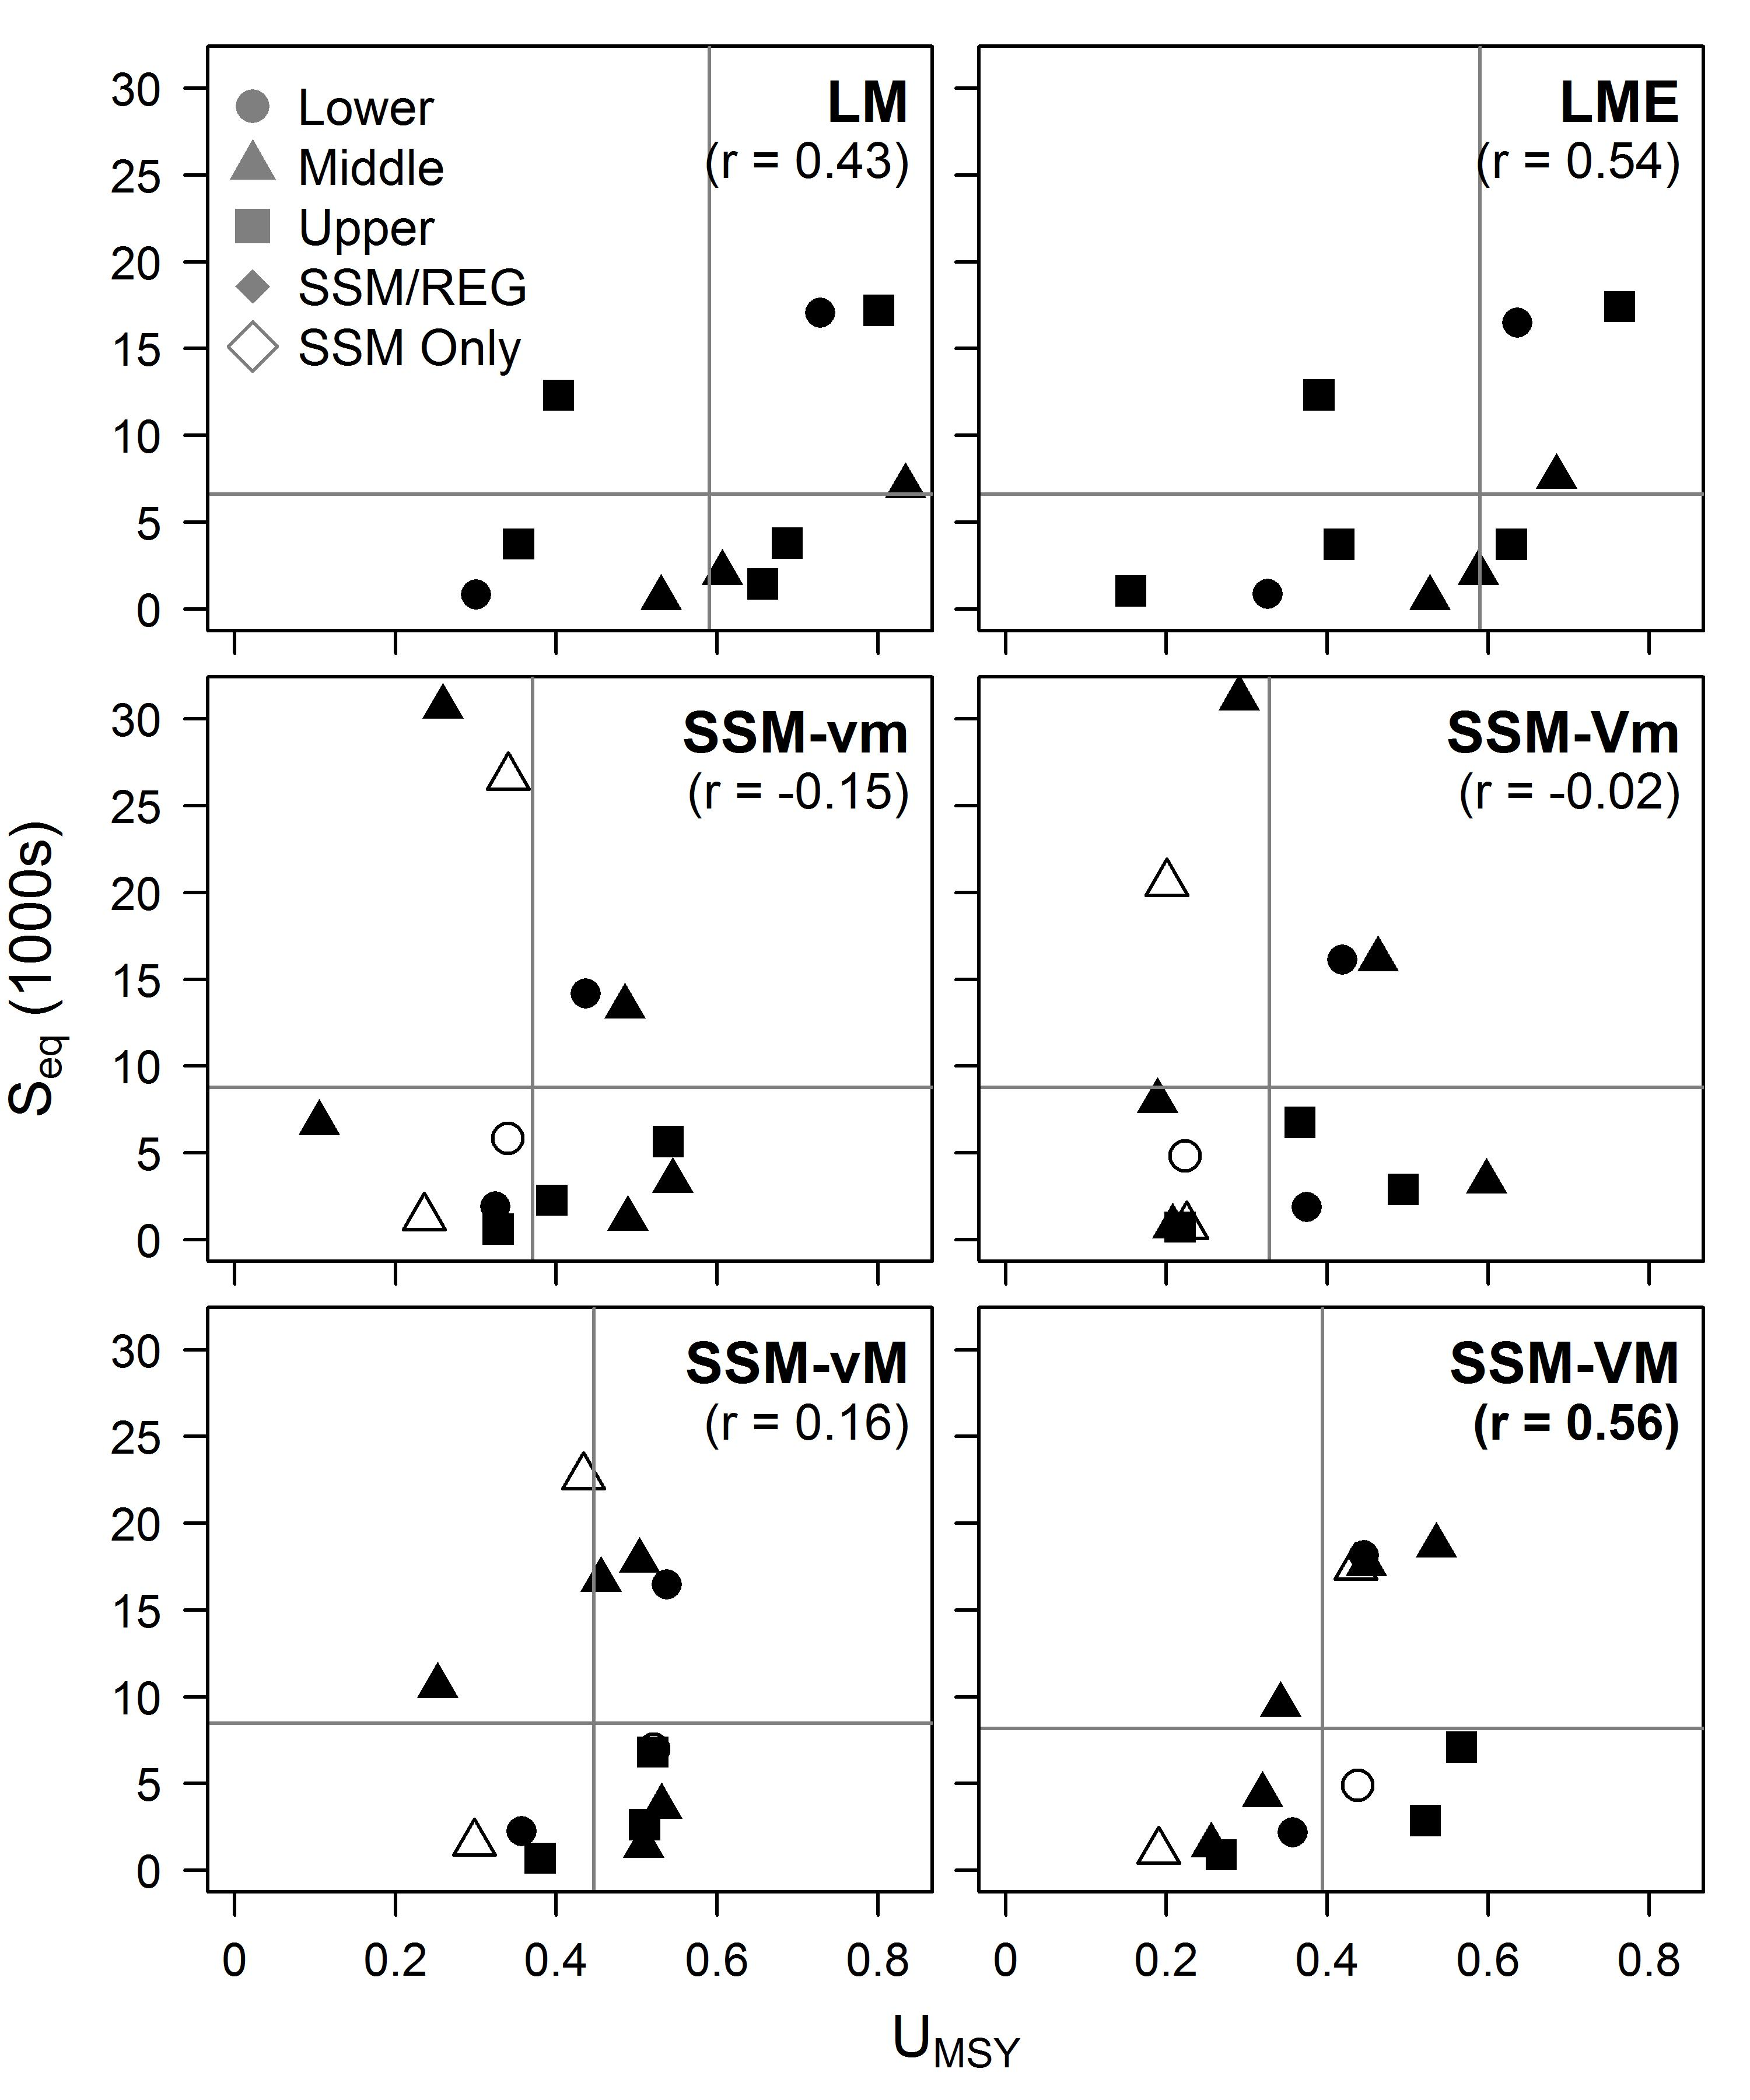
\includegraphics{img/Ch4/Size-v-Prod.jpg}
  \caption{Relationships between substock size and productivity as estimated by the six estimation approaches in the analysis. Symbol shapes denote the region within the Kuskokwim drainage the substock is located in and hollow symbols in the state-space models are substocks that could not be fitted by the regression approaches. The value in parentheses is Pearson's $r$ correlation coefficient; bold numbers indicate a significant correlation at $\alpha$ = 0.05.}
  \label{fig:size-v-prod}
\end{figure}

\clearpage

\begin{figure}
  \centering
  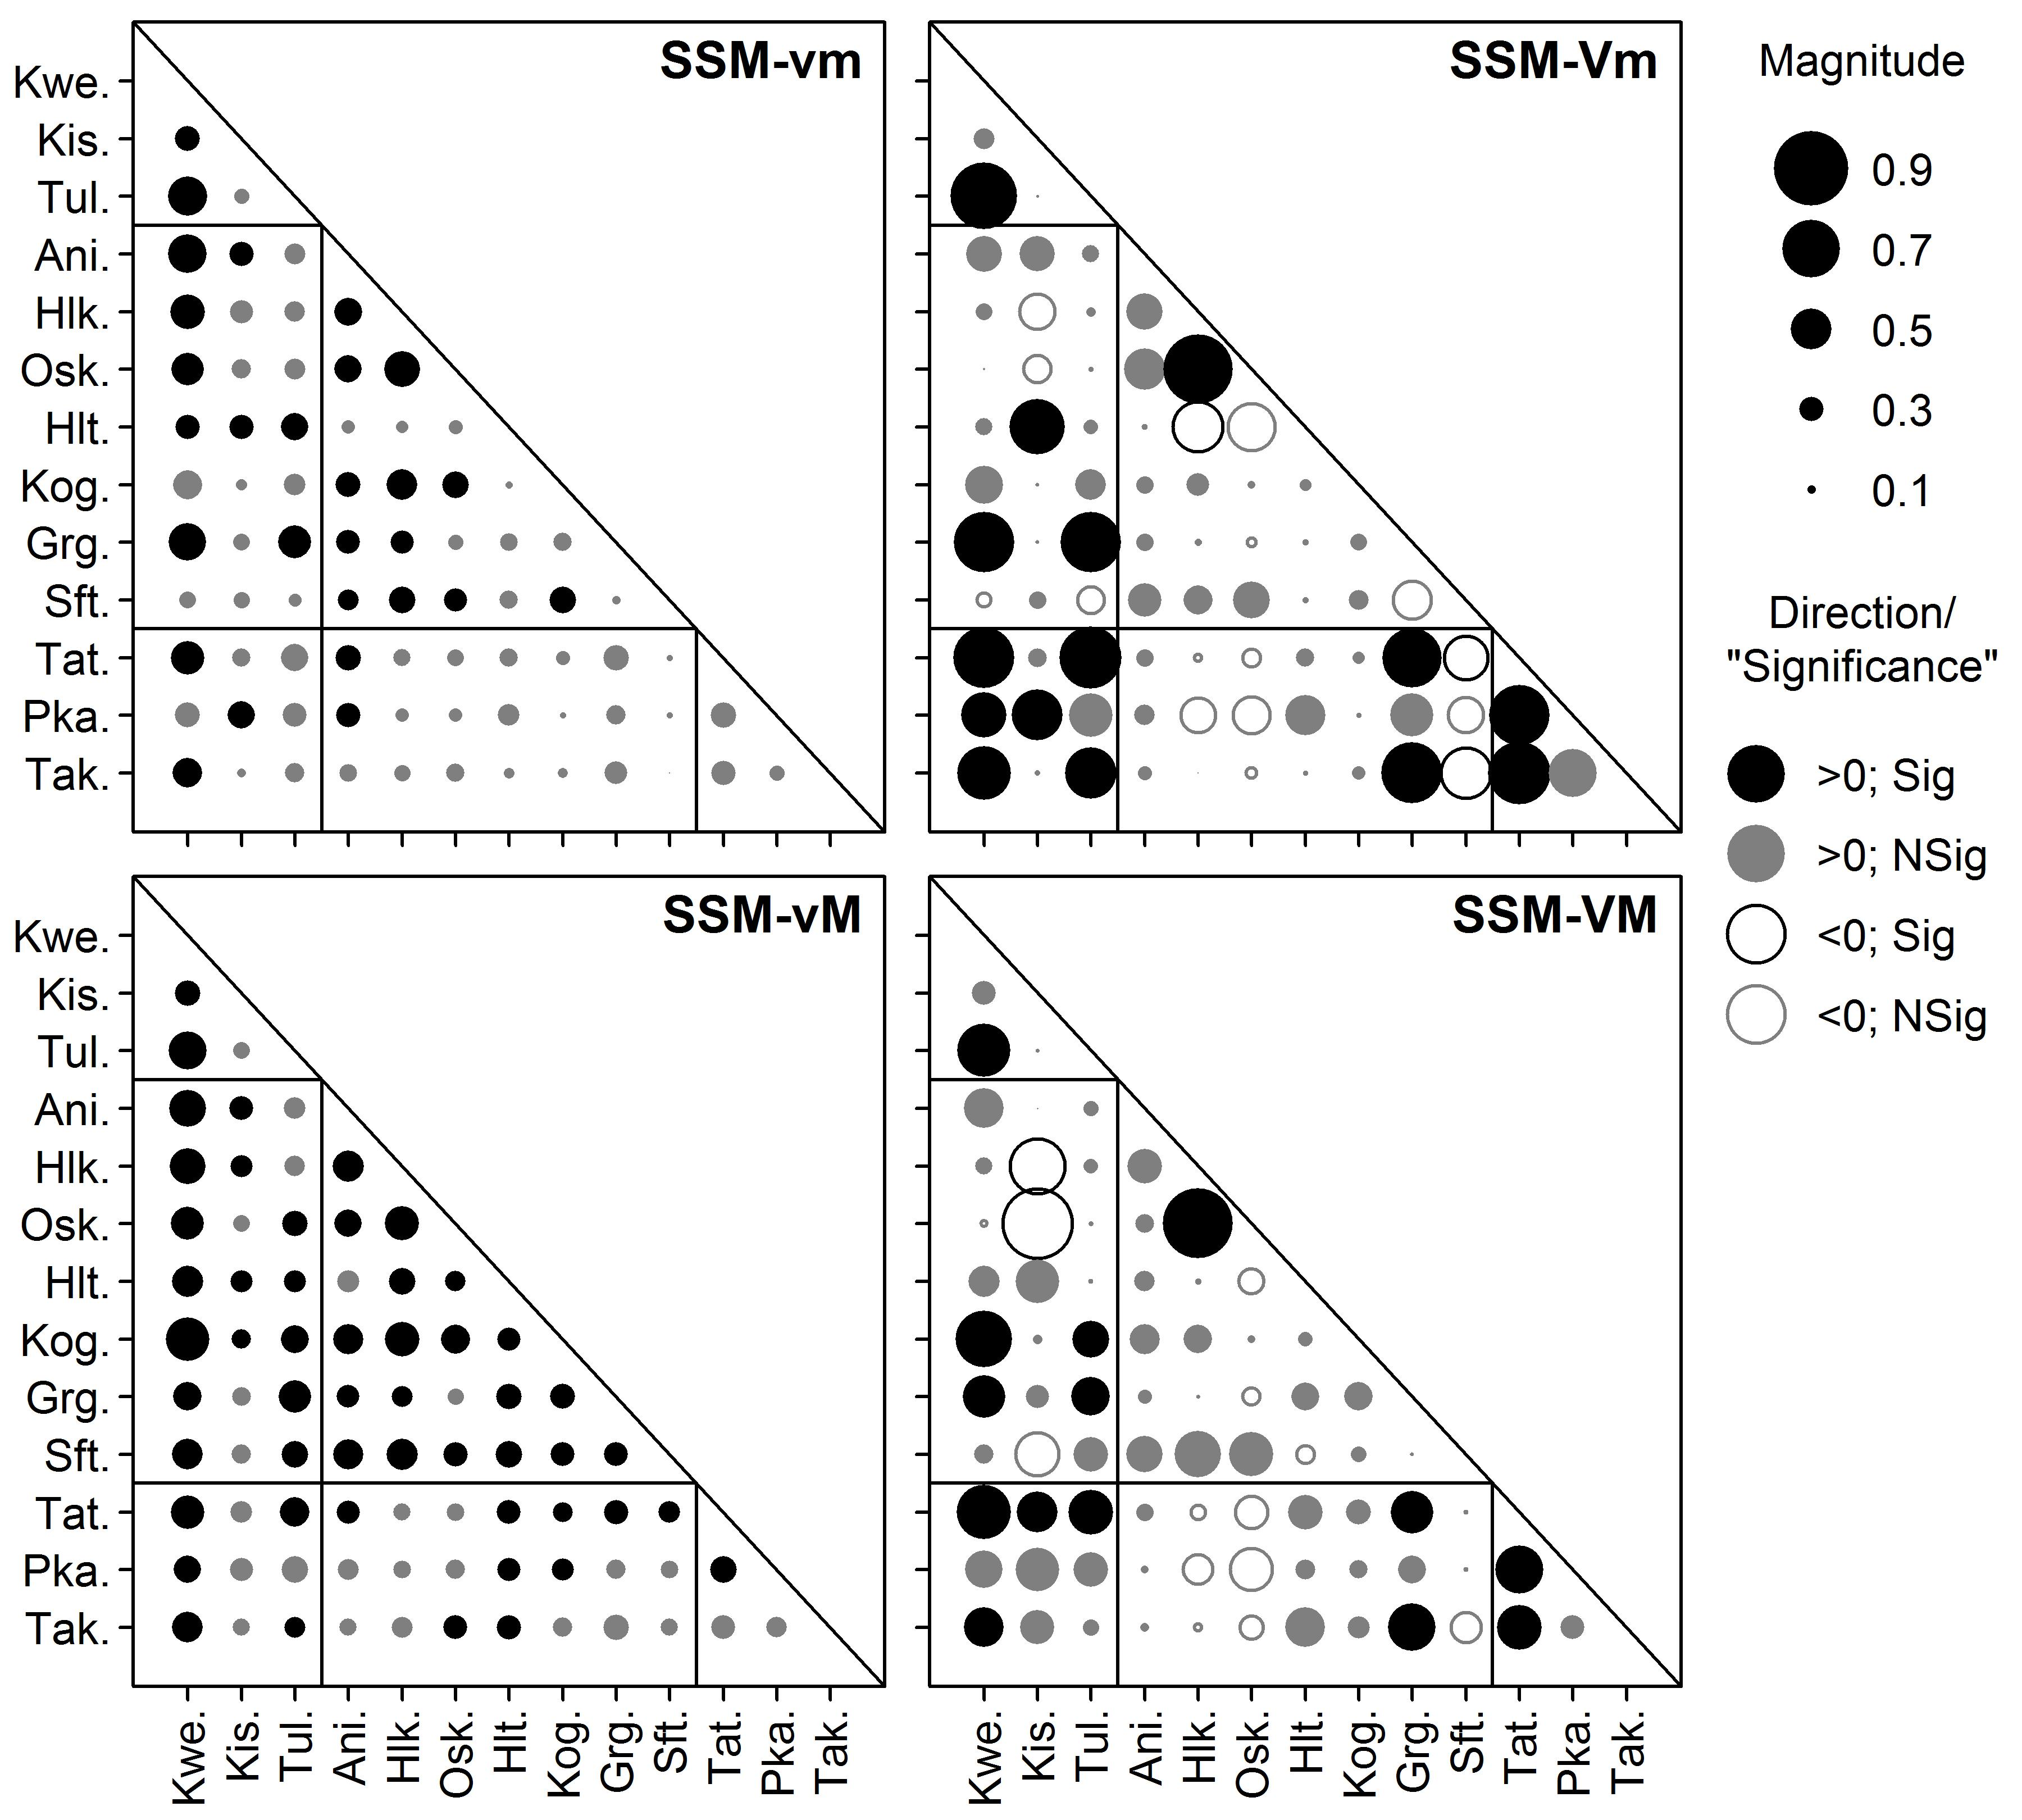
\includegraphics{img/Ch4/rhos.jpg}
  \caption{Correlation coefficients between recruitment residuals for each substock-pair. The size of each circle represents the magnitude of the correlation, color represents significance (whether 95\% credible interval includes 0), and fill represents directionality as described in the legend. Substocks are ordered from downriver to upriver on both axes, and vertical/horizontal lines denote the boundaries between lower, middle, and upper river substocks.}
  \label{fig:rhos}
\end{figure}

\clearpage

\begin{figure}
  \centering
  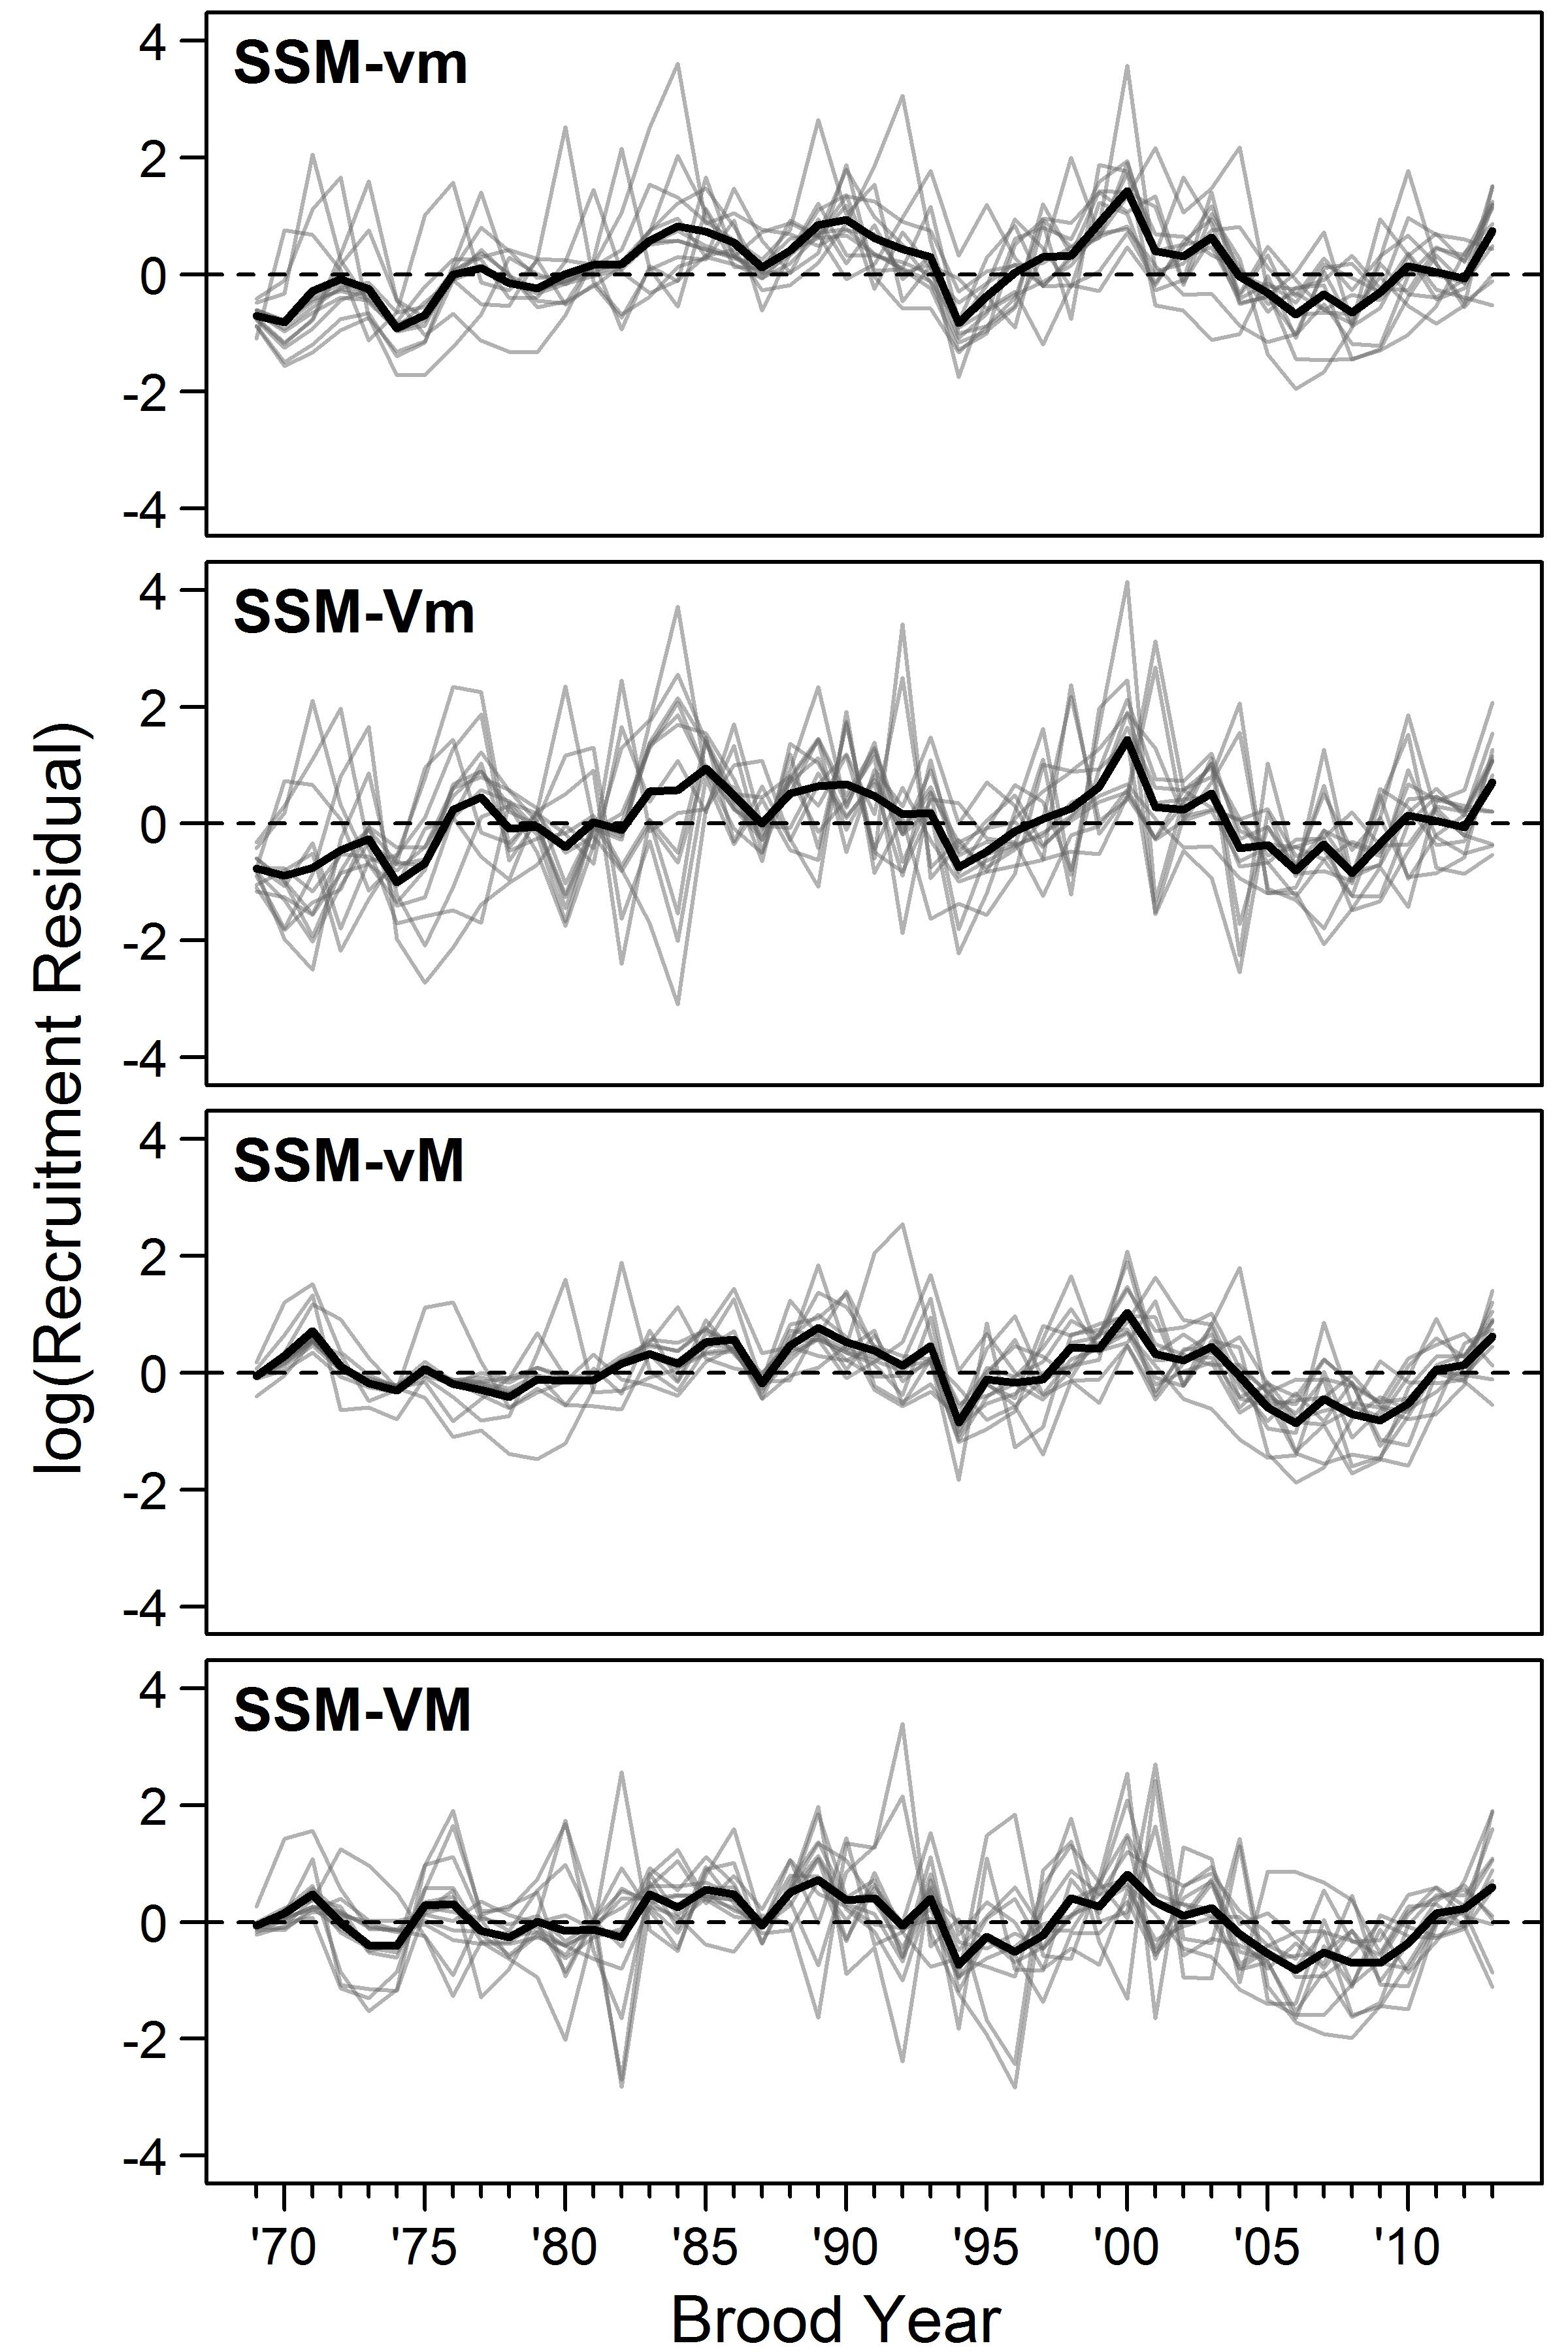
\includegraphics{img/Ch4/log-resids.jpg}
  \caption{Time series of recruitment residuals for each substock under each of the four state-space models. Substock-specific time series are represented by grey lines and the average across substocks within a brood year are represented by the thick black line. A dashed line at zero (no error) is provided for reference.}
  \label{fig:log-resids}
\end{figure}

\clearpage

\begin{figure}
  \centering
  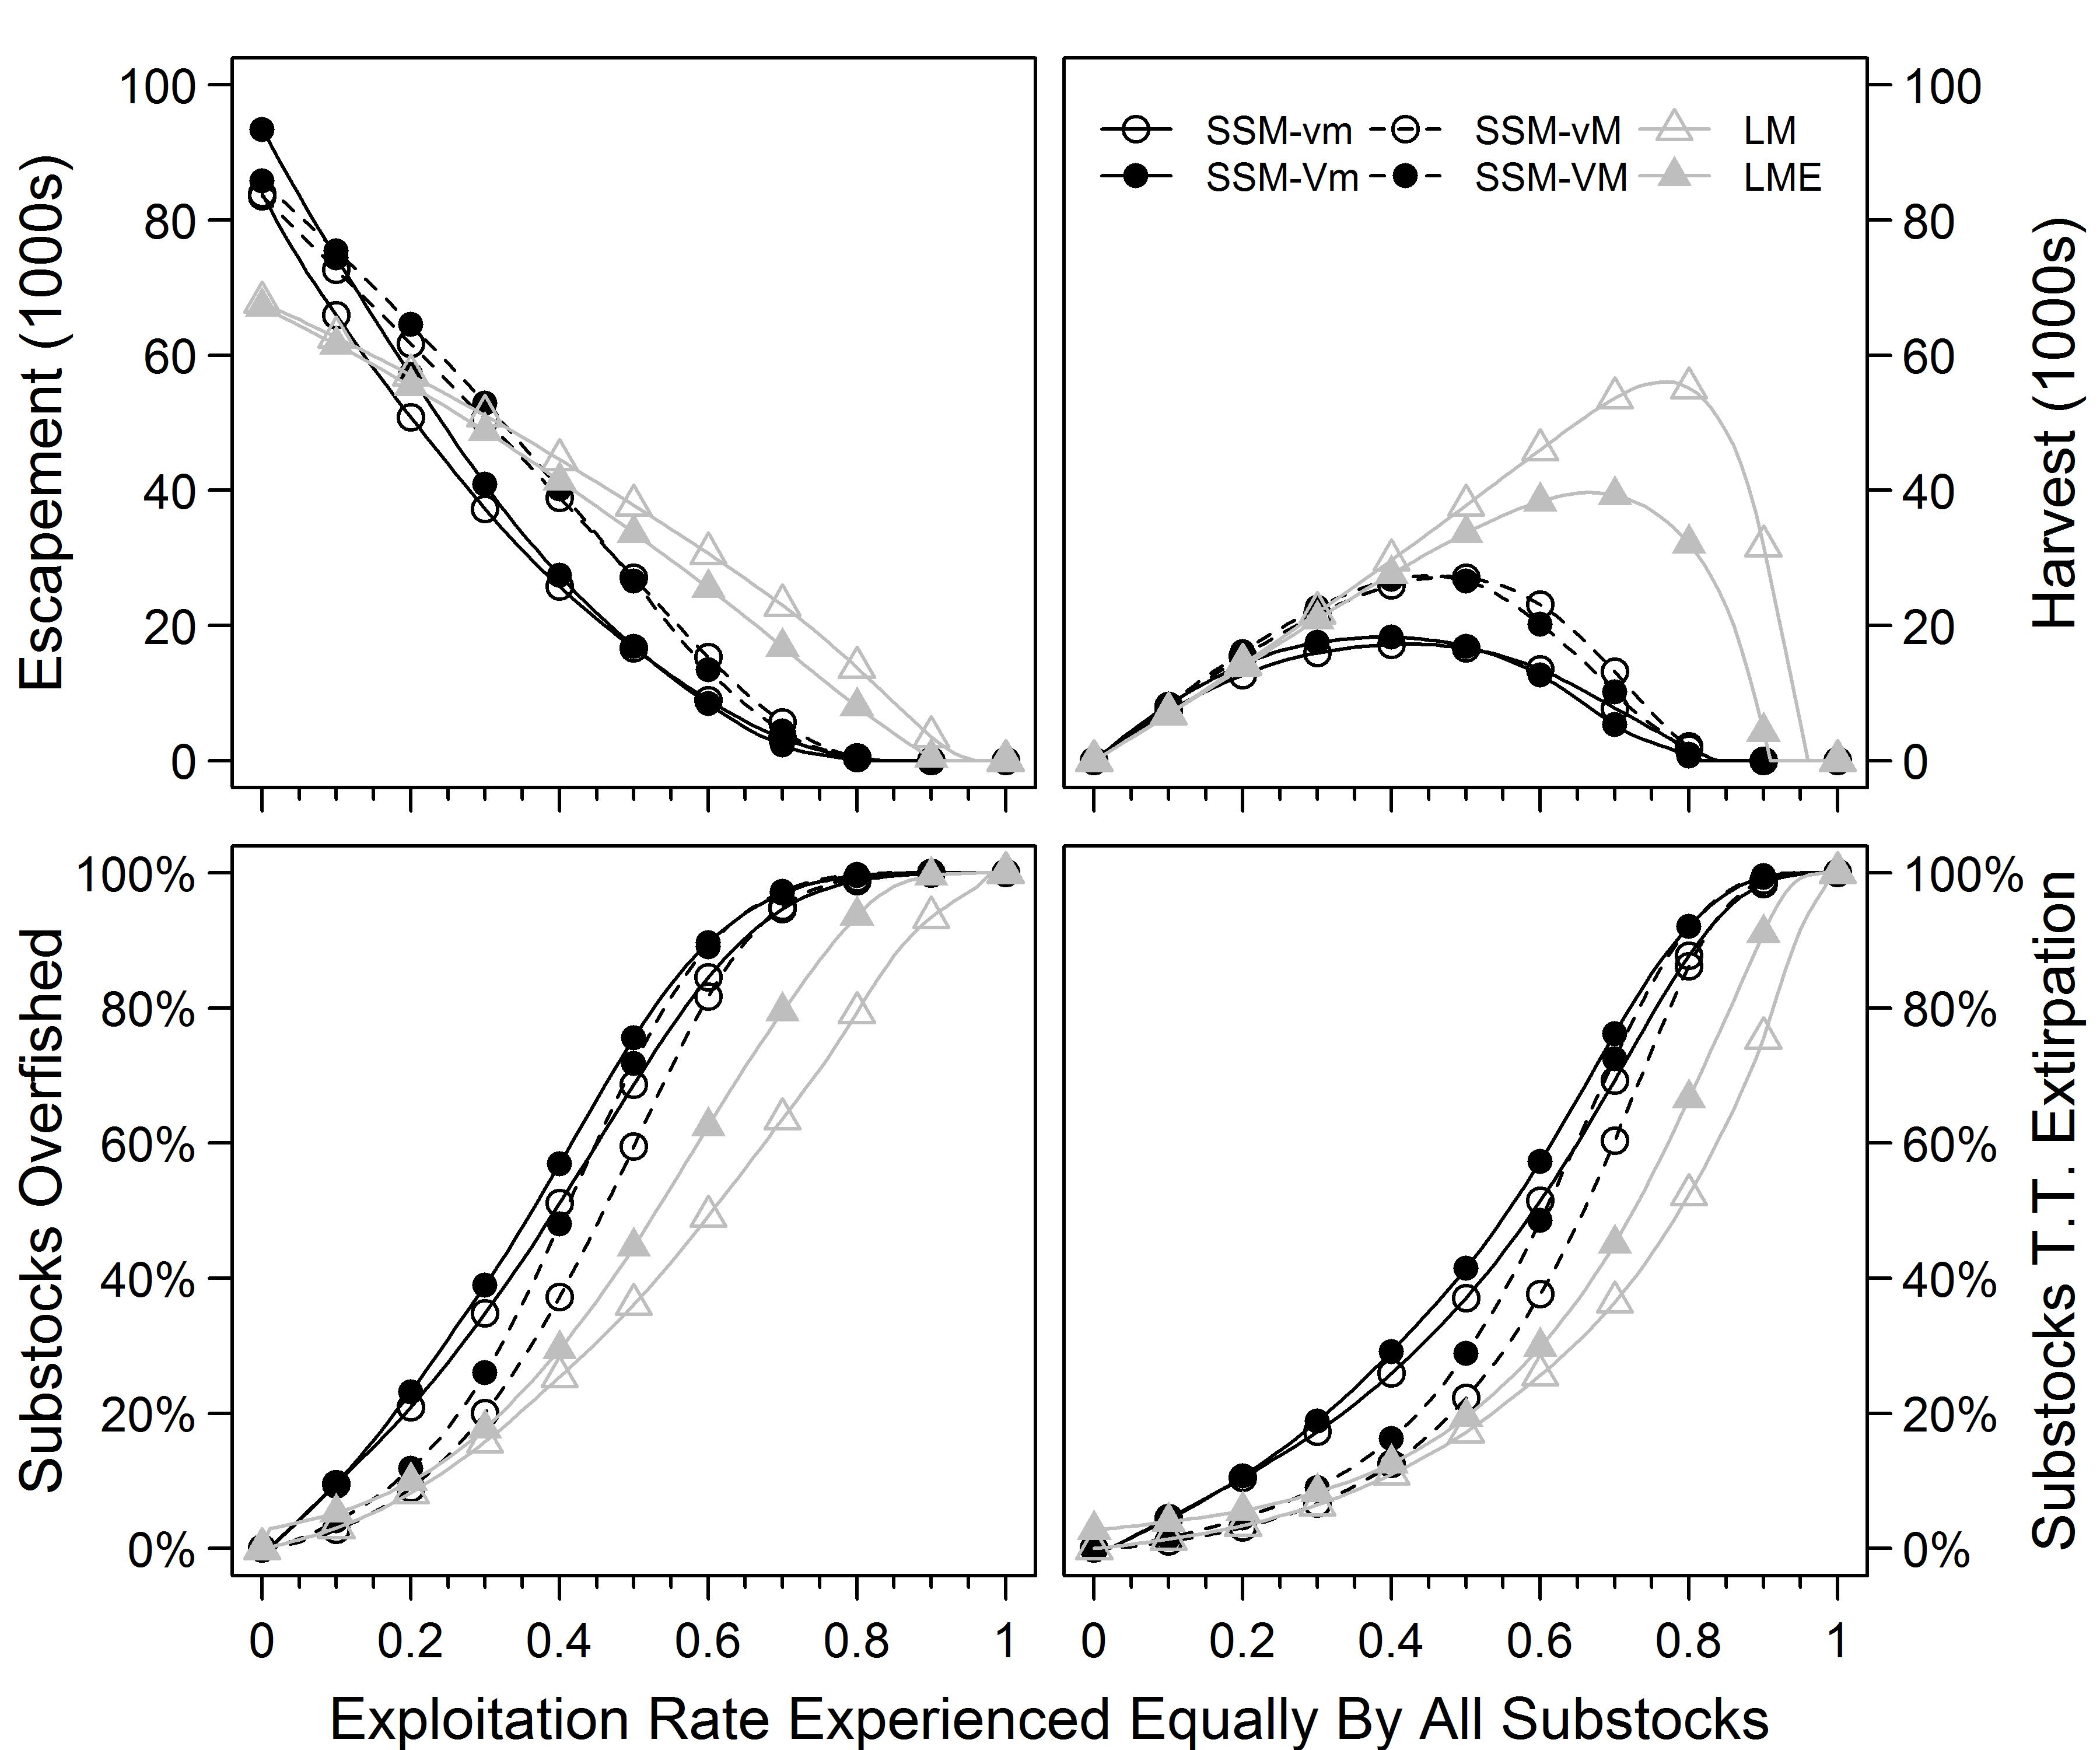
\includegraphics{img/Ch4/kusko-eq-states.jpg}
  \caption{Visualization of harvest-biodiversity trade-offs based on equilibrium states (escapement and harvest) of the aggregate stock and the percentage of substocks expected to be in an undesirable state as a function of the exploitation rate under the assumption that all substocks are fished at the same rate. Overfished is defined here as $U > U_{\text{MSY},j}$. ``T.T.'' stands for ``trending toward'', and represents the case where equilibrium escapement would be $\le 0$. To facilitate comparisons with the regression approaches (grey lines/triangles), the three substocks with insufficient data for fitting regression models were excluded from summaries of the state-space models (black triangles/circles).} 
  \label{fig:kusko-eq-states}
\end{figure}

\clearpage

\begin{figure}
  \centering
  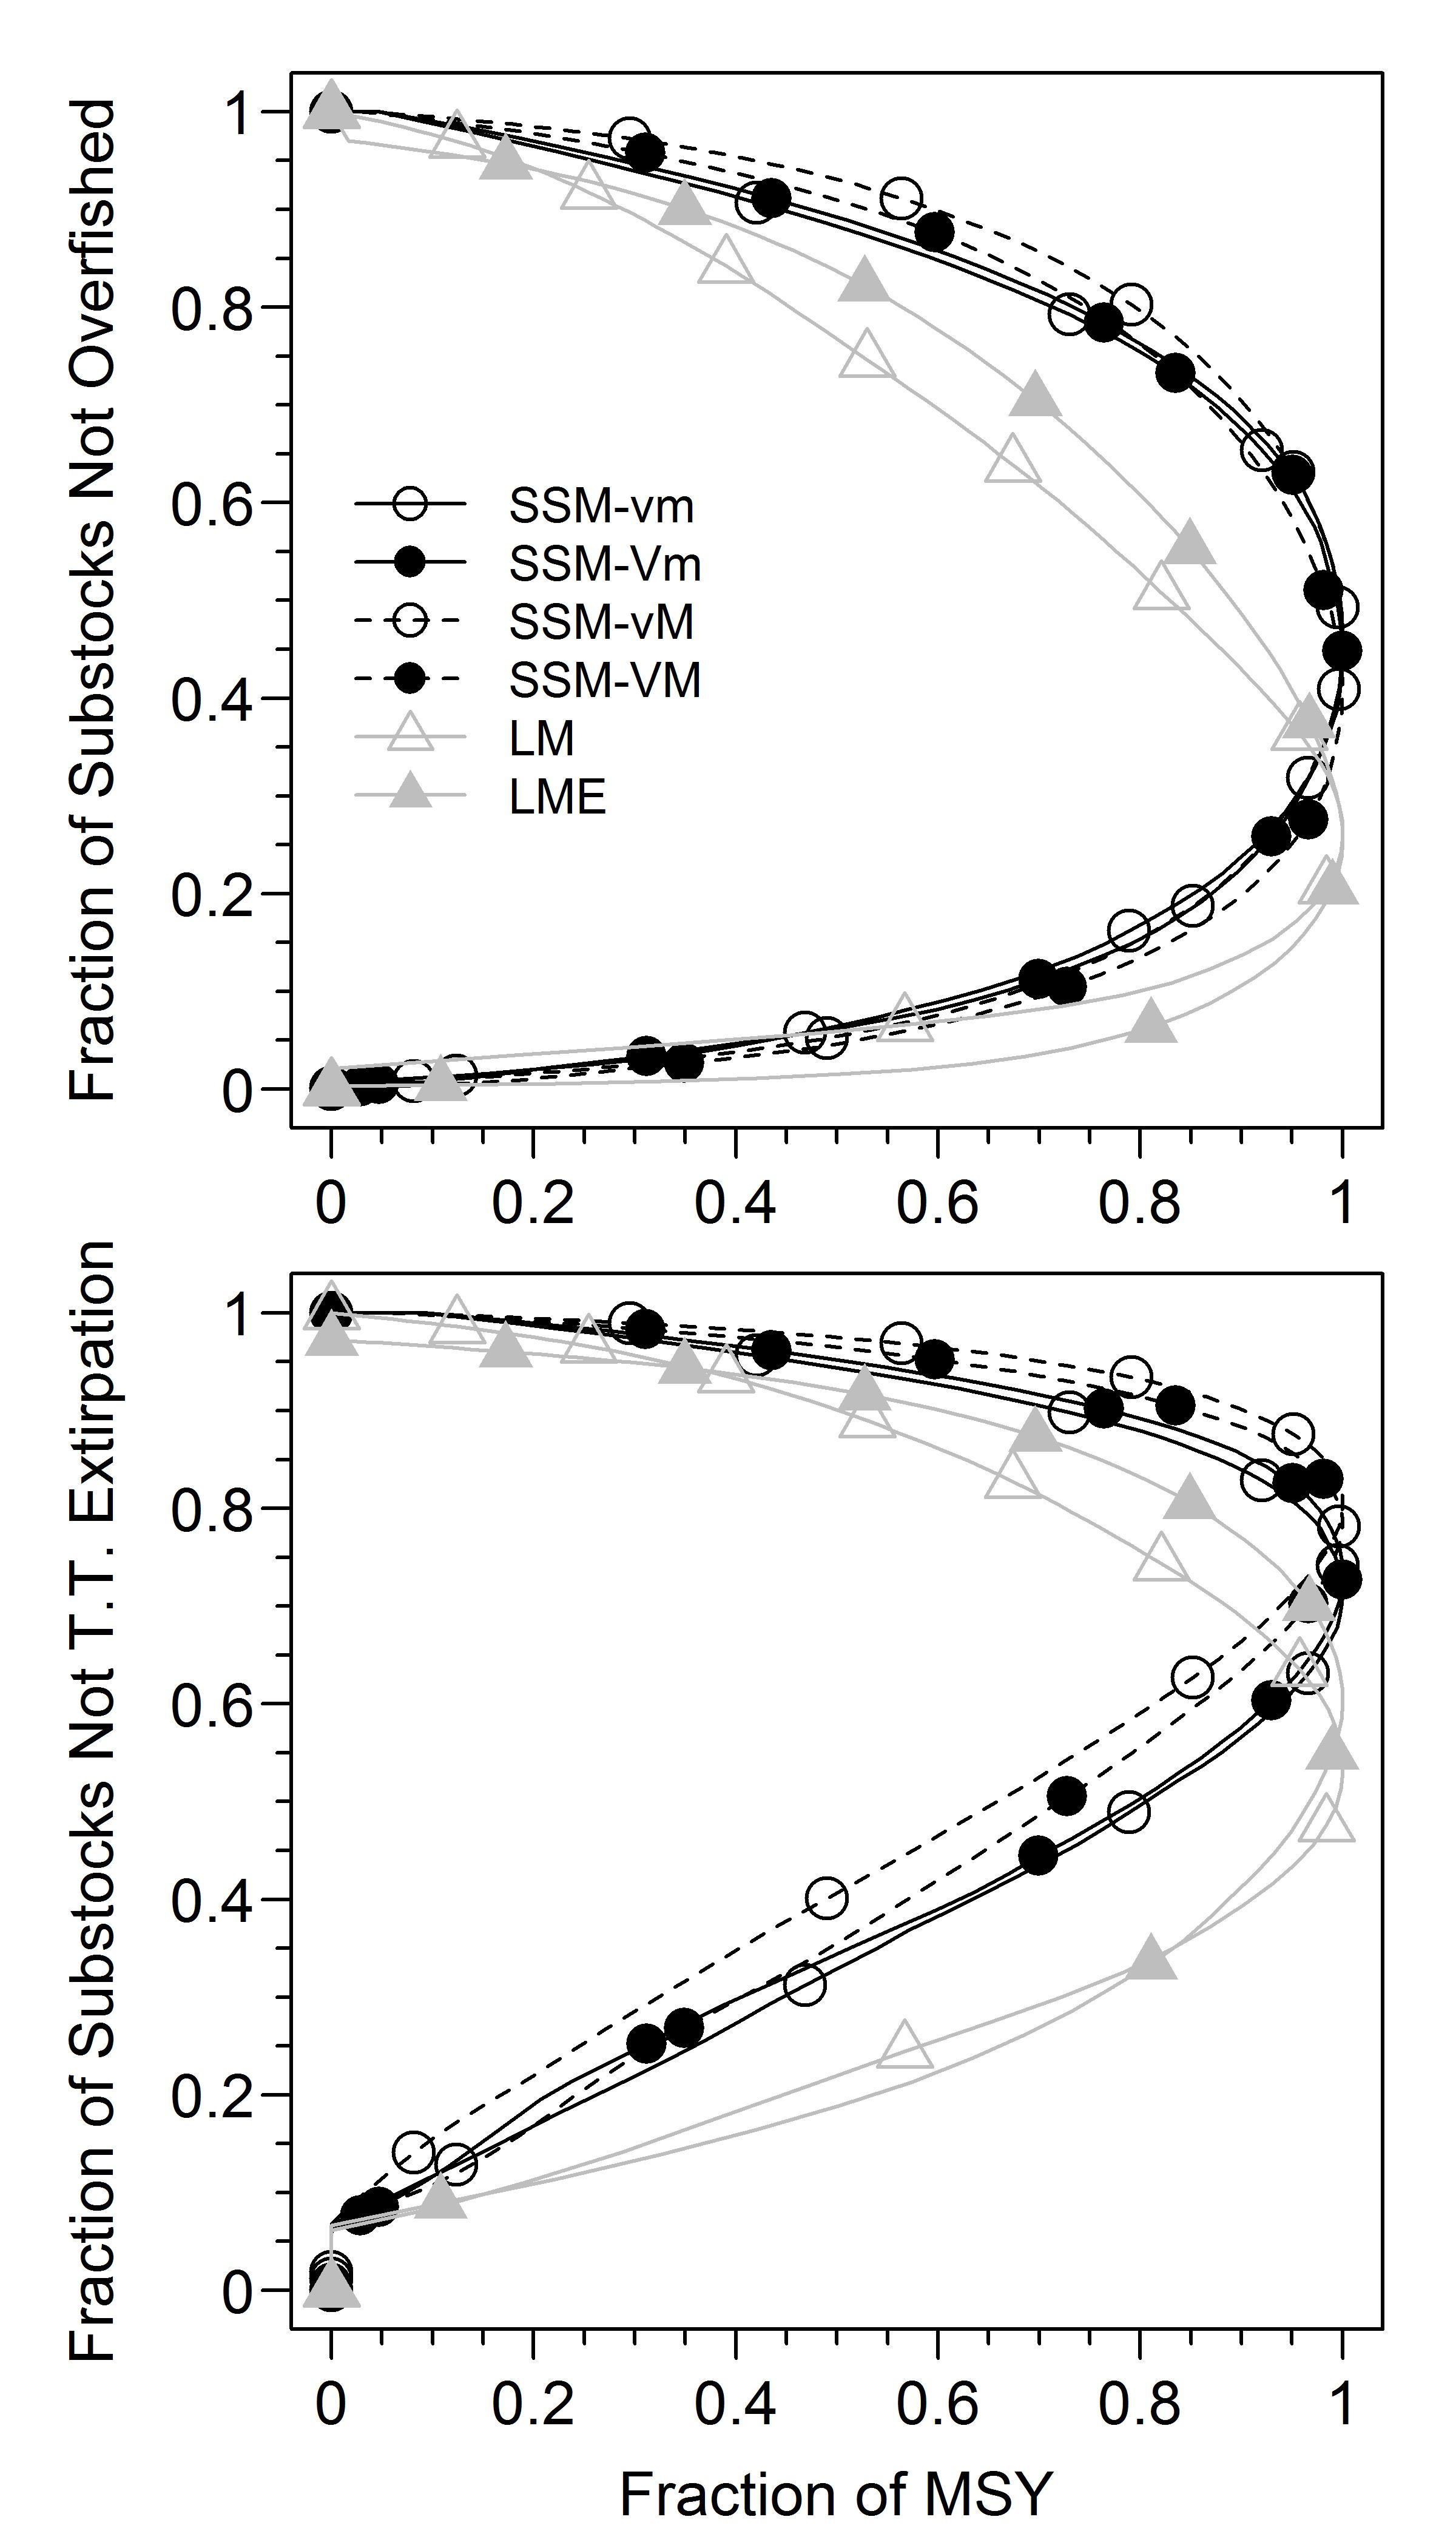
\includegraphics{img/Ch4/kusko-trade-offs.jpg}
  \caption{Alternative (and more direct than Figure \ref{fig:kusko-eq-states}) visualization of harvest-biodiversity trade-offs for monitored Kuskokwim River Chinook salmon substocks. The conditions of overfished and trending towards extinction are the same as defined in Figure \ref{fig:kusko-eq-states}. These figures should be interpreted by determining how the value of the biodiversity objective (\textit{y}-axis; expressed as the fraction of substocks that would not be in the undesirable condition) must be reduced to increase the value of the harvest objective (\textit{y}-axis; expressed as a fraction of the maximum sustainable yield). To facilitate comparisons with the regression approaches (grey lines/triangles), the three substocks with insufficient data for fitting regression models were excluded from summaries of the state-space models (black triangles/circles). All symbols represent increasing exploitation rates in increments of 0.1 as you move down the \textit{y}-axis.}
  \label{fig:kusko-trade-offs}
\end{figure}

\clearpage

\begin{figure}
  \centering
  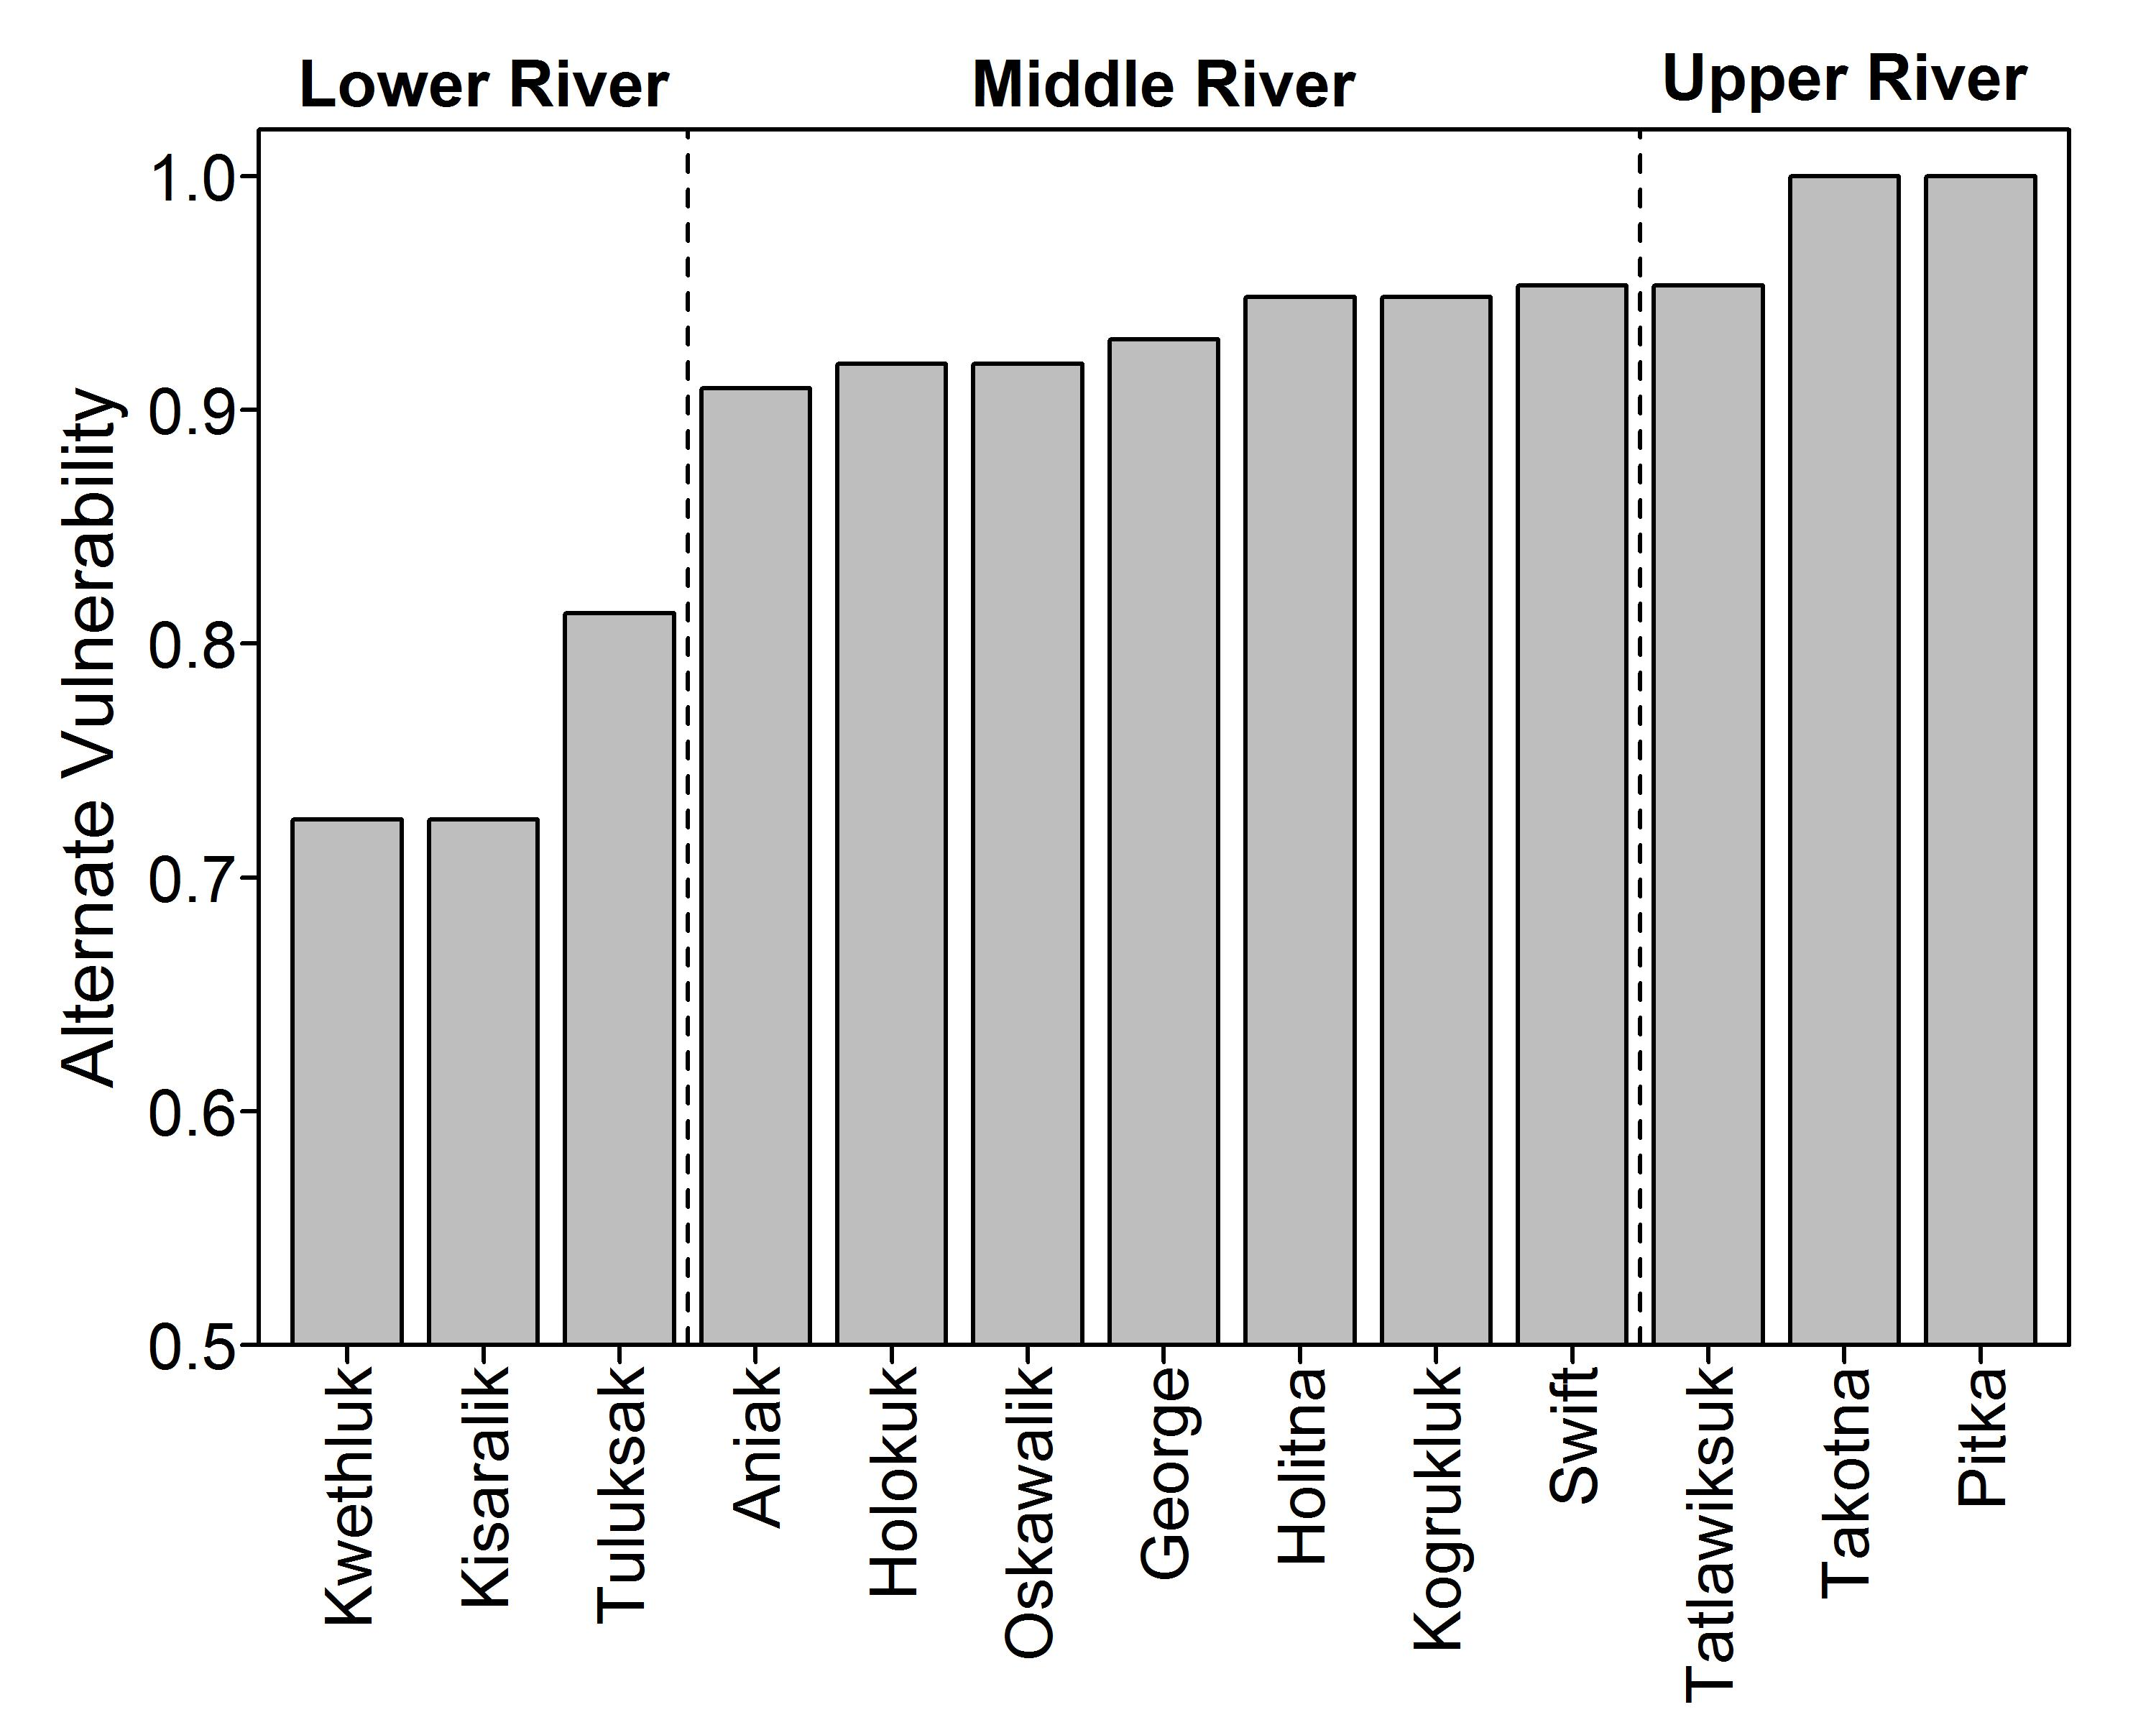
\includegraphics{img/Ch4/alt-vuln-fig.jpg}
  \caption{Alternative vulnerability schedule ($v_j$) used in a sensitivity analysis of the state-space models. Vulnerabilities were obtained by determining the fraction of total fishing households the individual substocks must swim past in order to reach their respective natal spawning grounds. Substocks are ordered from downstream to upstream.}
  \label{fig:alt-vuln-fig}
\end{figure}

\clearpage

\begin{figure}
  \centering
  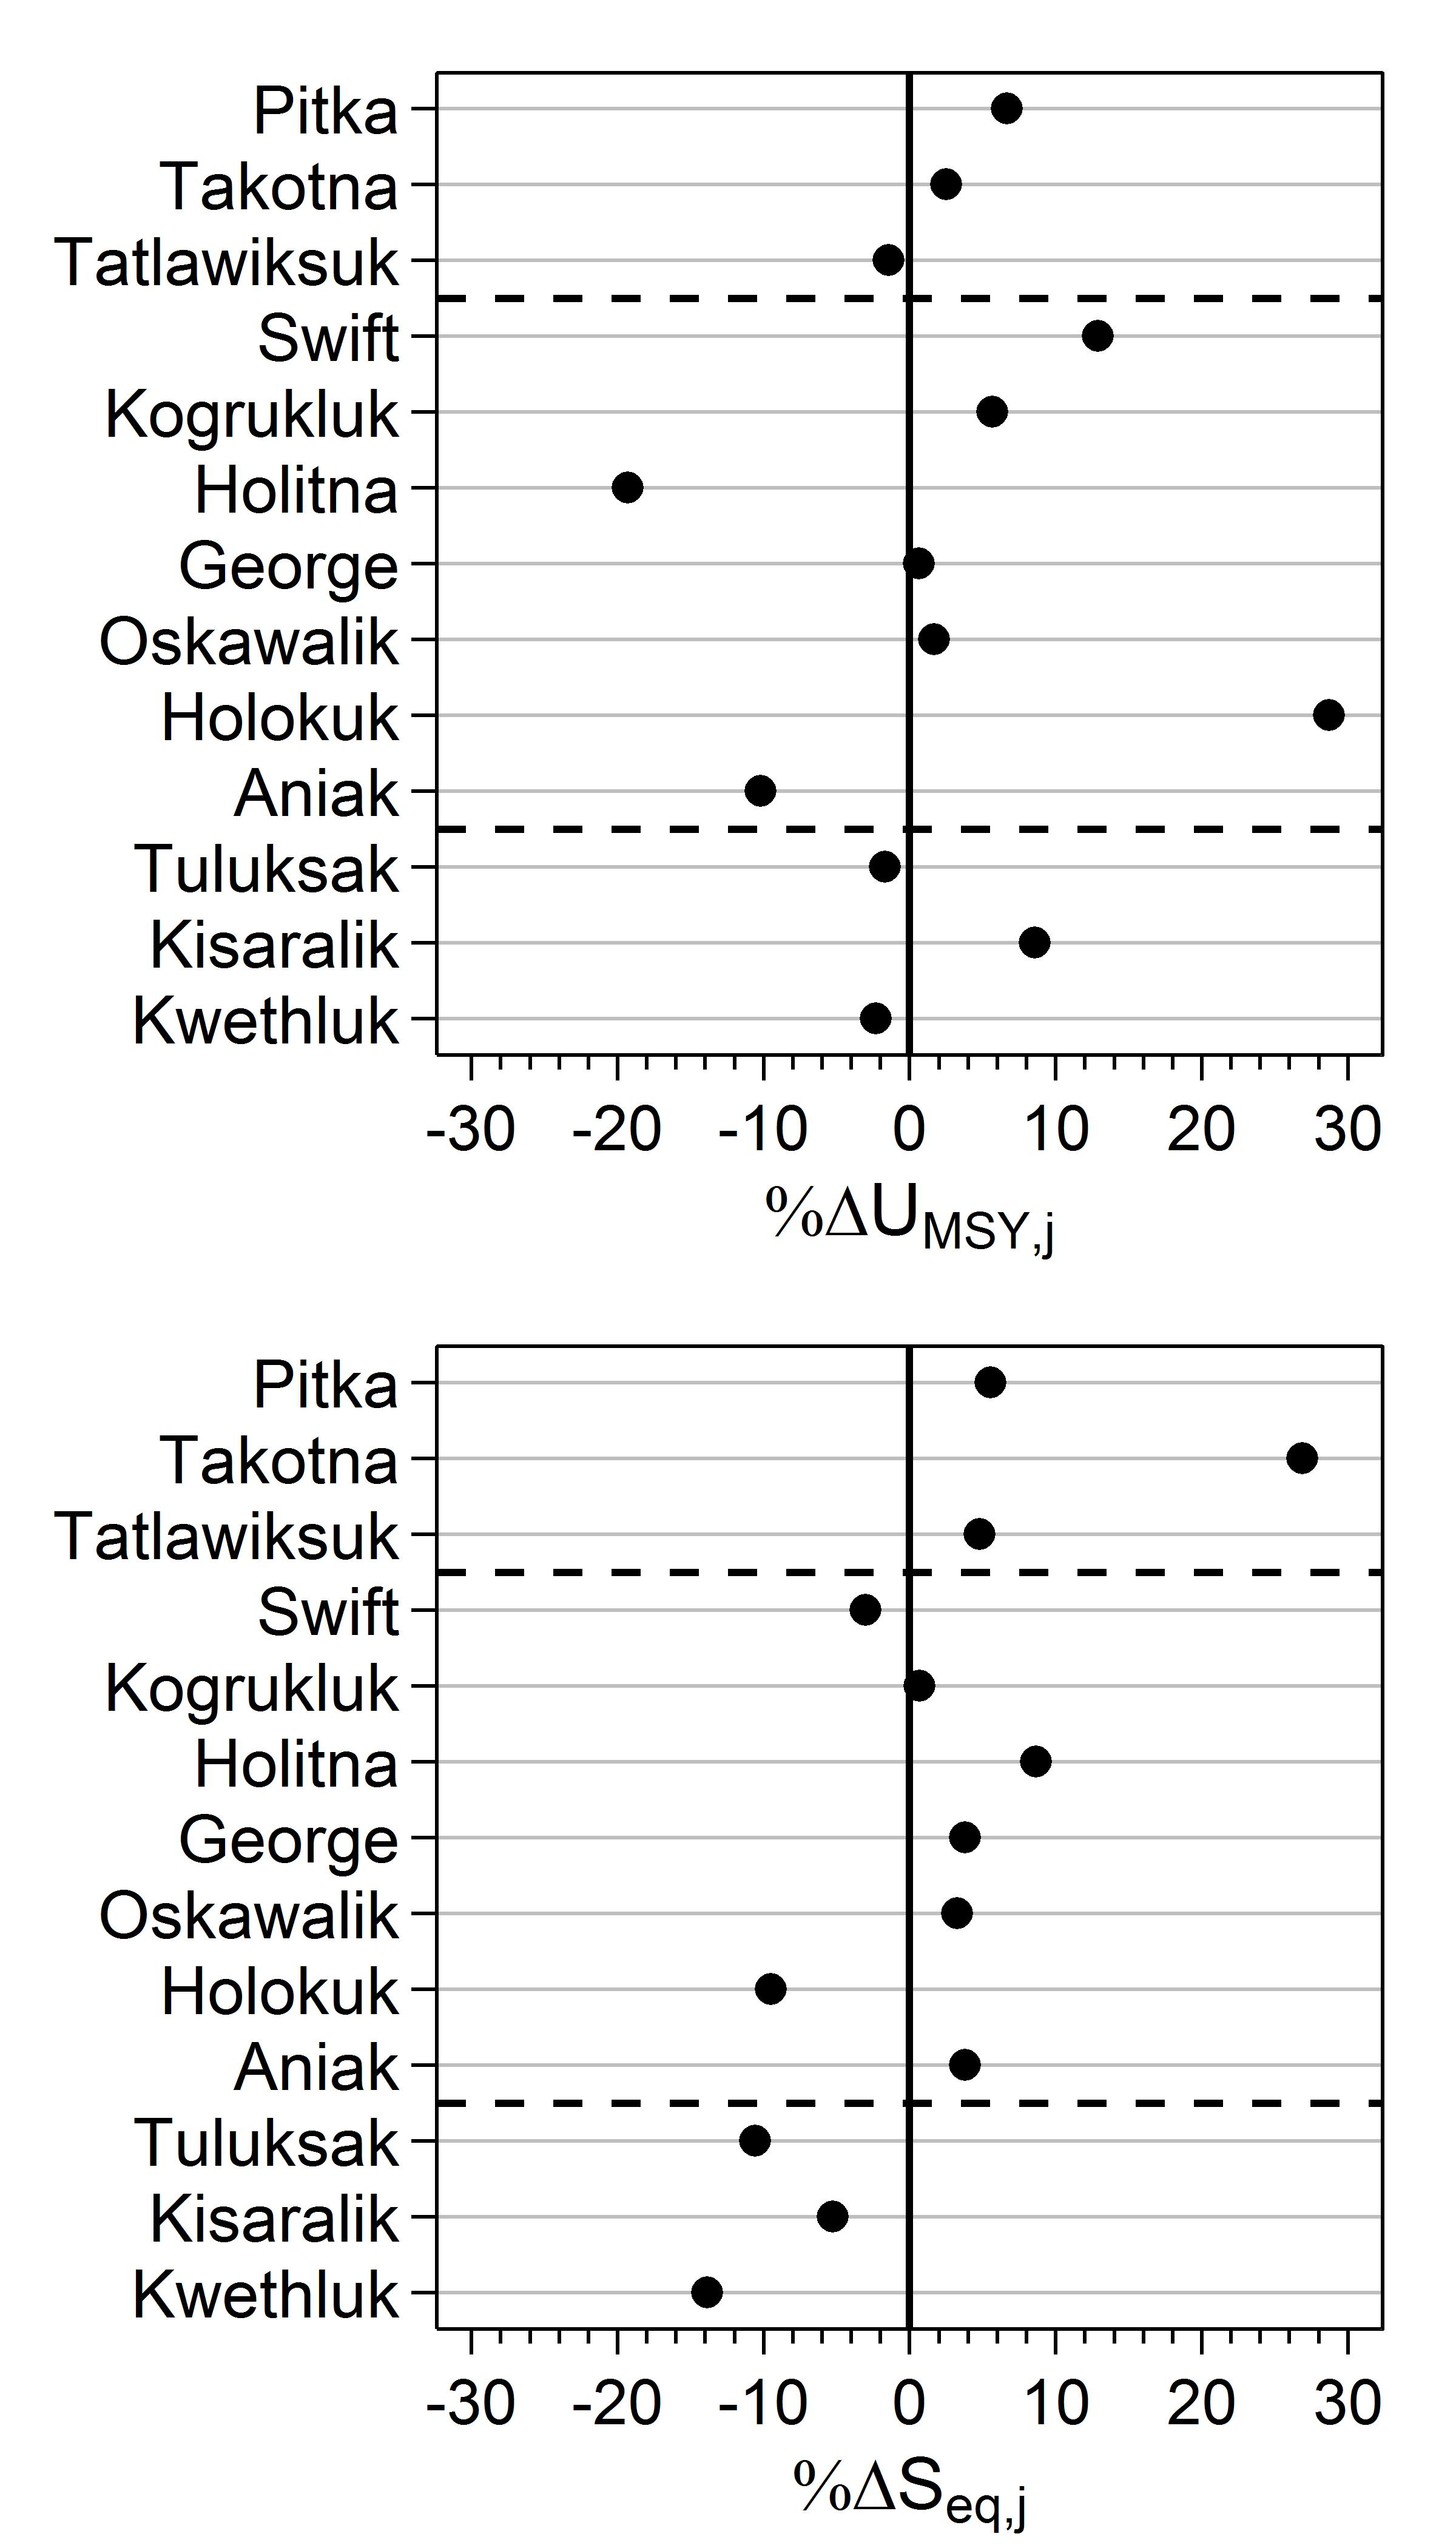
\includegraphics{img/Ch4/alt-vuln-ests.jpg}
  \caption{Percent change in substock-specific population quantities between the alternative and default vulnerability schedules. Positive differences indicate that the alternative estimates were larger than the default estimates. Estimates are displayed for SSM-VM only, all other state-space models returned similar differences.}
  \label{fig:alt-vuln-ests}
\end{figure}

\clearpage

\begin{figure}
  \centering
  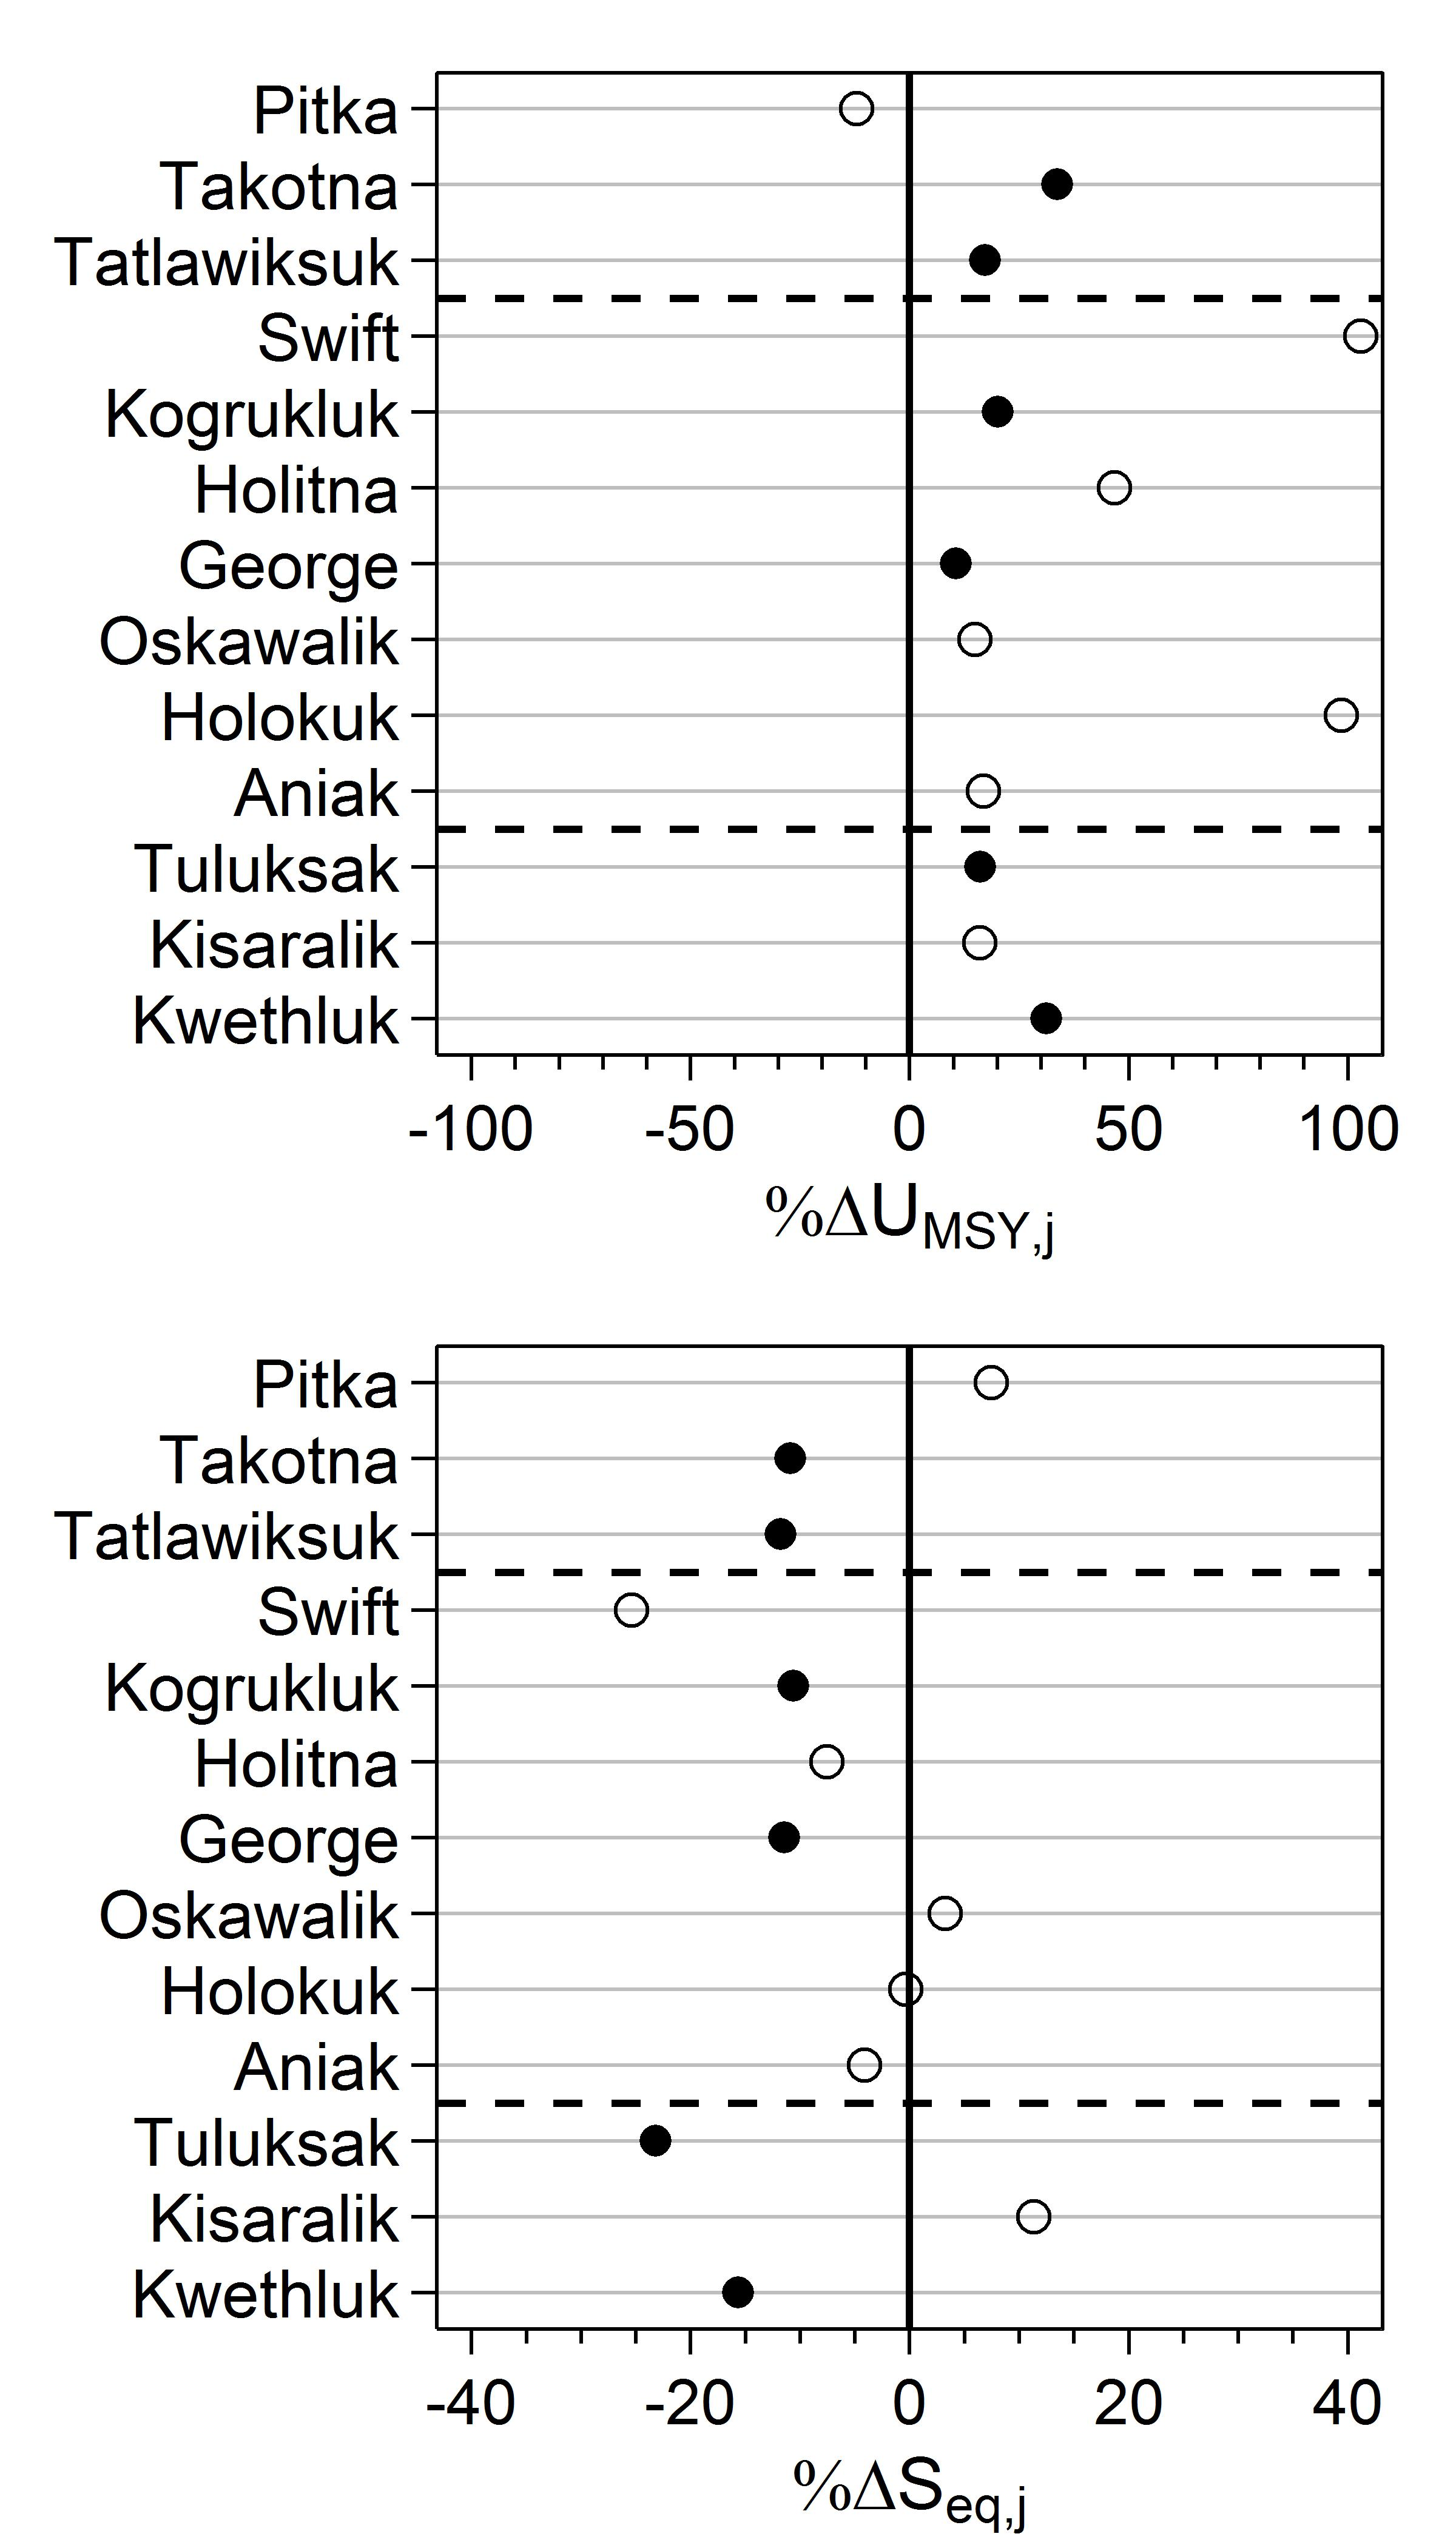
\includegraphics{img/Ch4/alt-ess-ests.jpg}
  \caption{Percent change in substock-specific population quantities estimates between the alternative and default age composition weighting schemes. Positive differences indicate that the alternative estimates were larger than the default estimates. Filled symbols denote substocks with age composition data. Estimates are displayed for SSM-VM only, all other state-space models returned similar differences.}
  \label{fig:alt-ess-ests}
\end{figure}

\clearpage

\begin{figure}
  \centering
  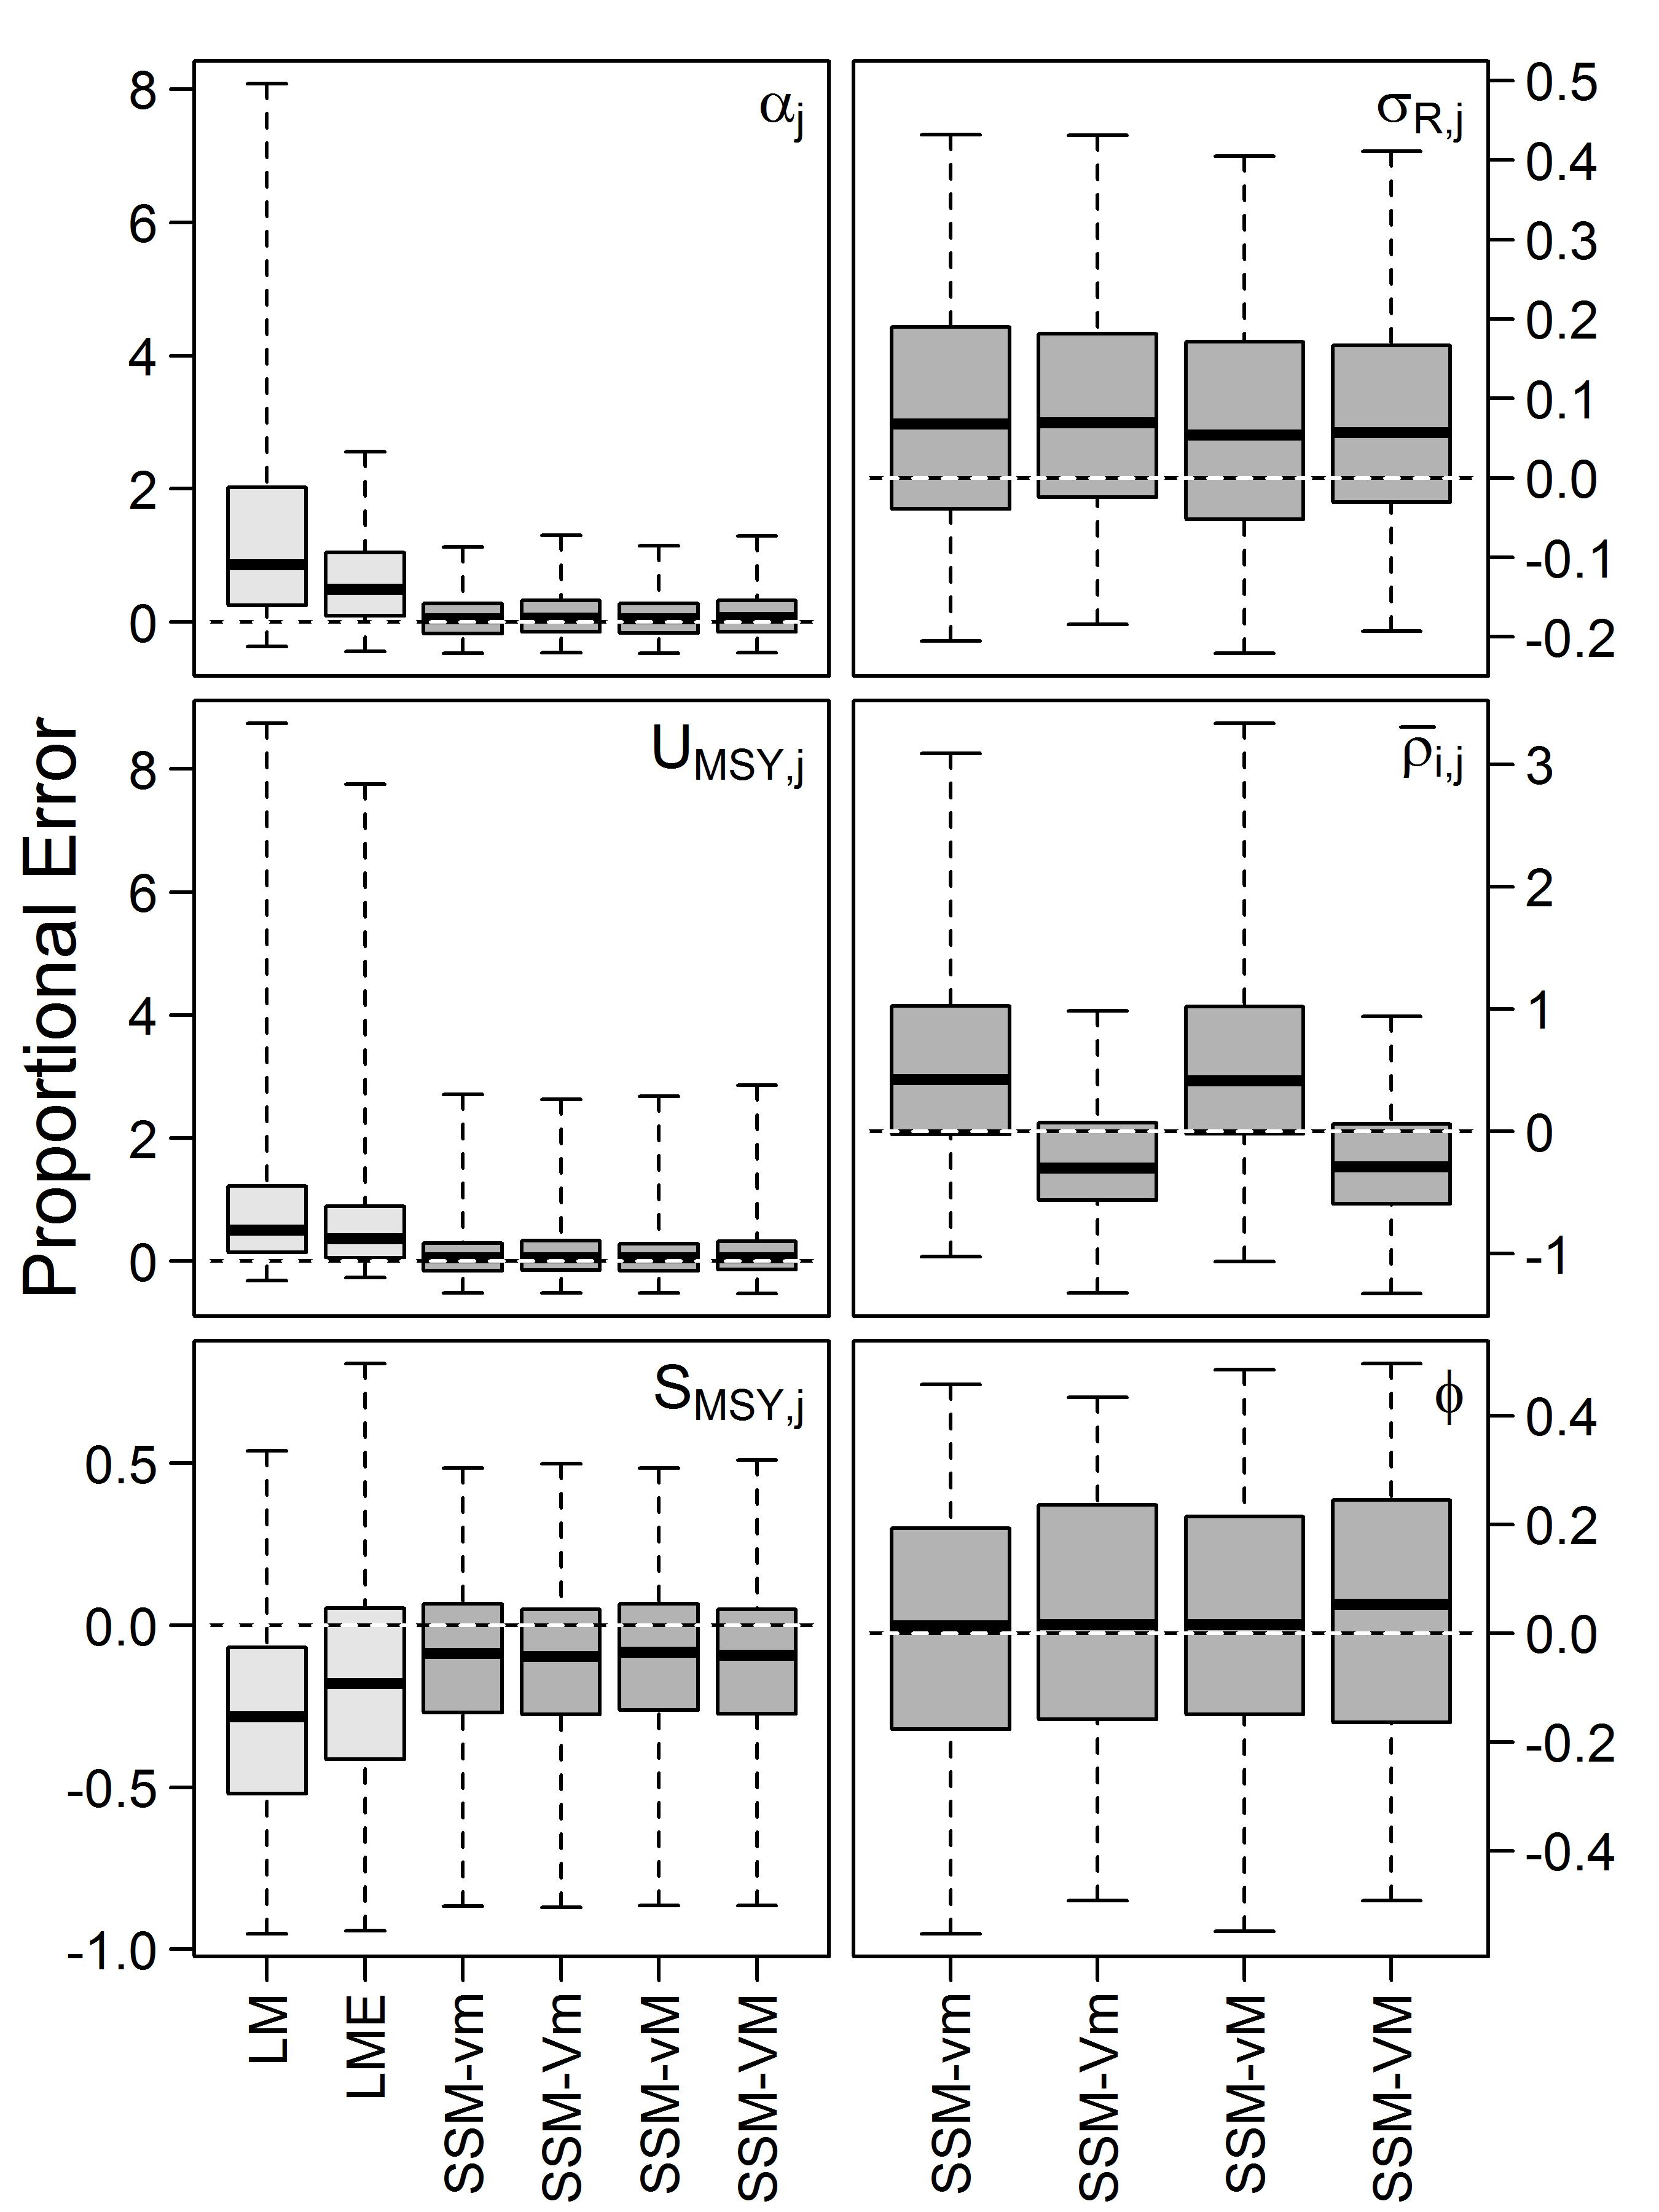
\includegraphics{img/Ch4/param-bias.jpg}
  \caption{Central tendency and variability in proportional error for some parameters in the multi-stock spawner-recruit models from the simulation-estimation trials. Point estimates used were posterior medians.}
  \label{fig:param-bias}
\end{figure}

\clearpage

\begin{figure}
  \centering
  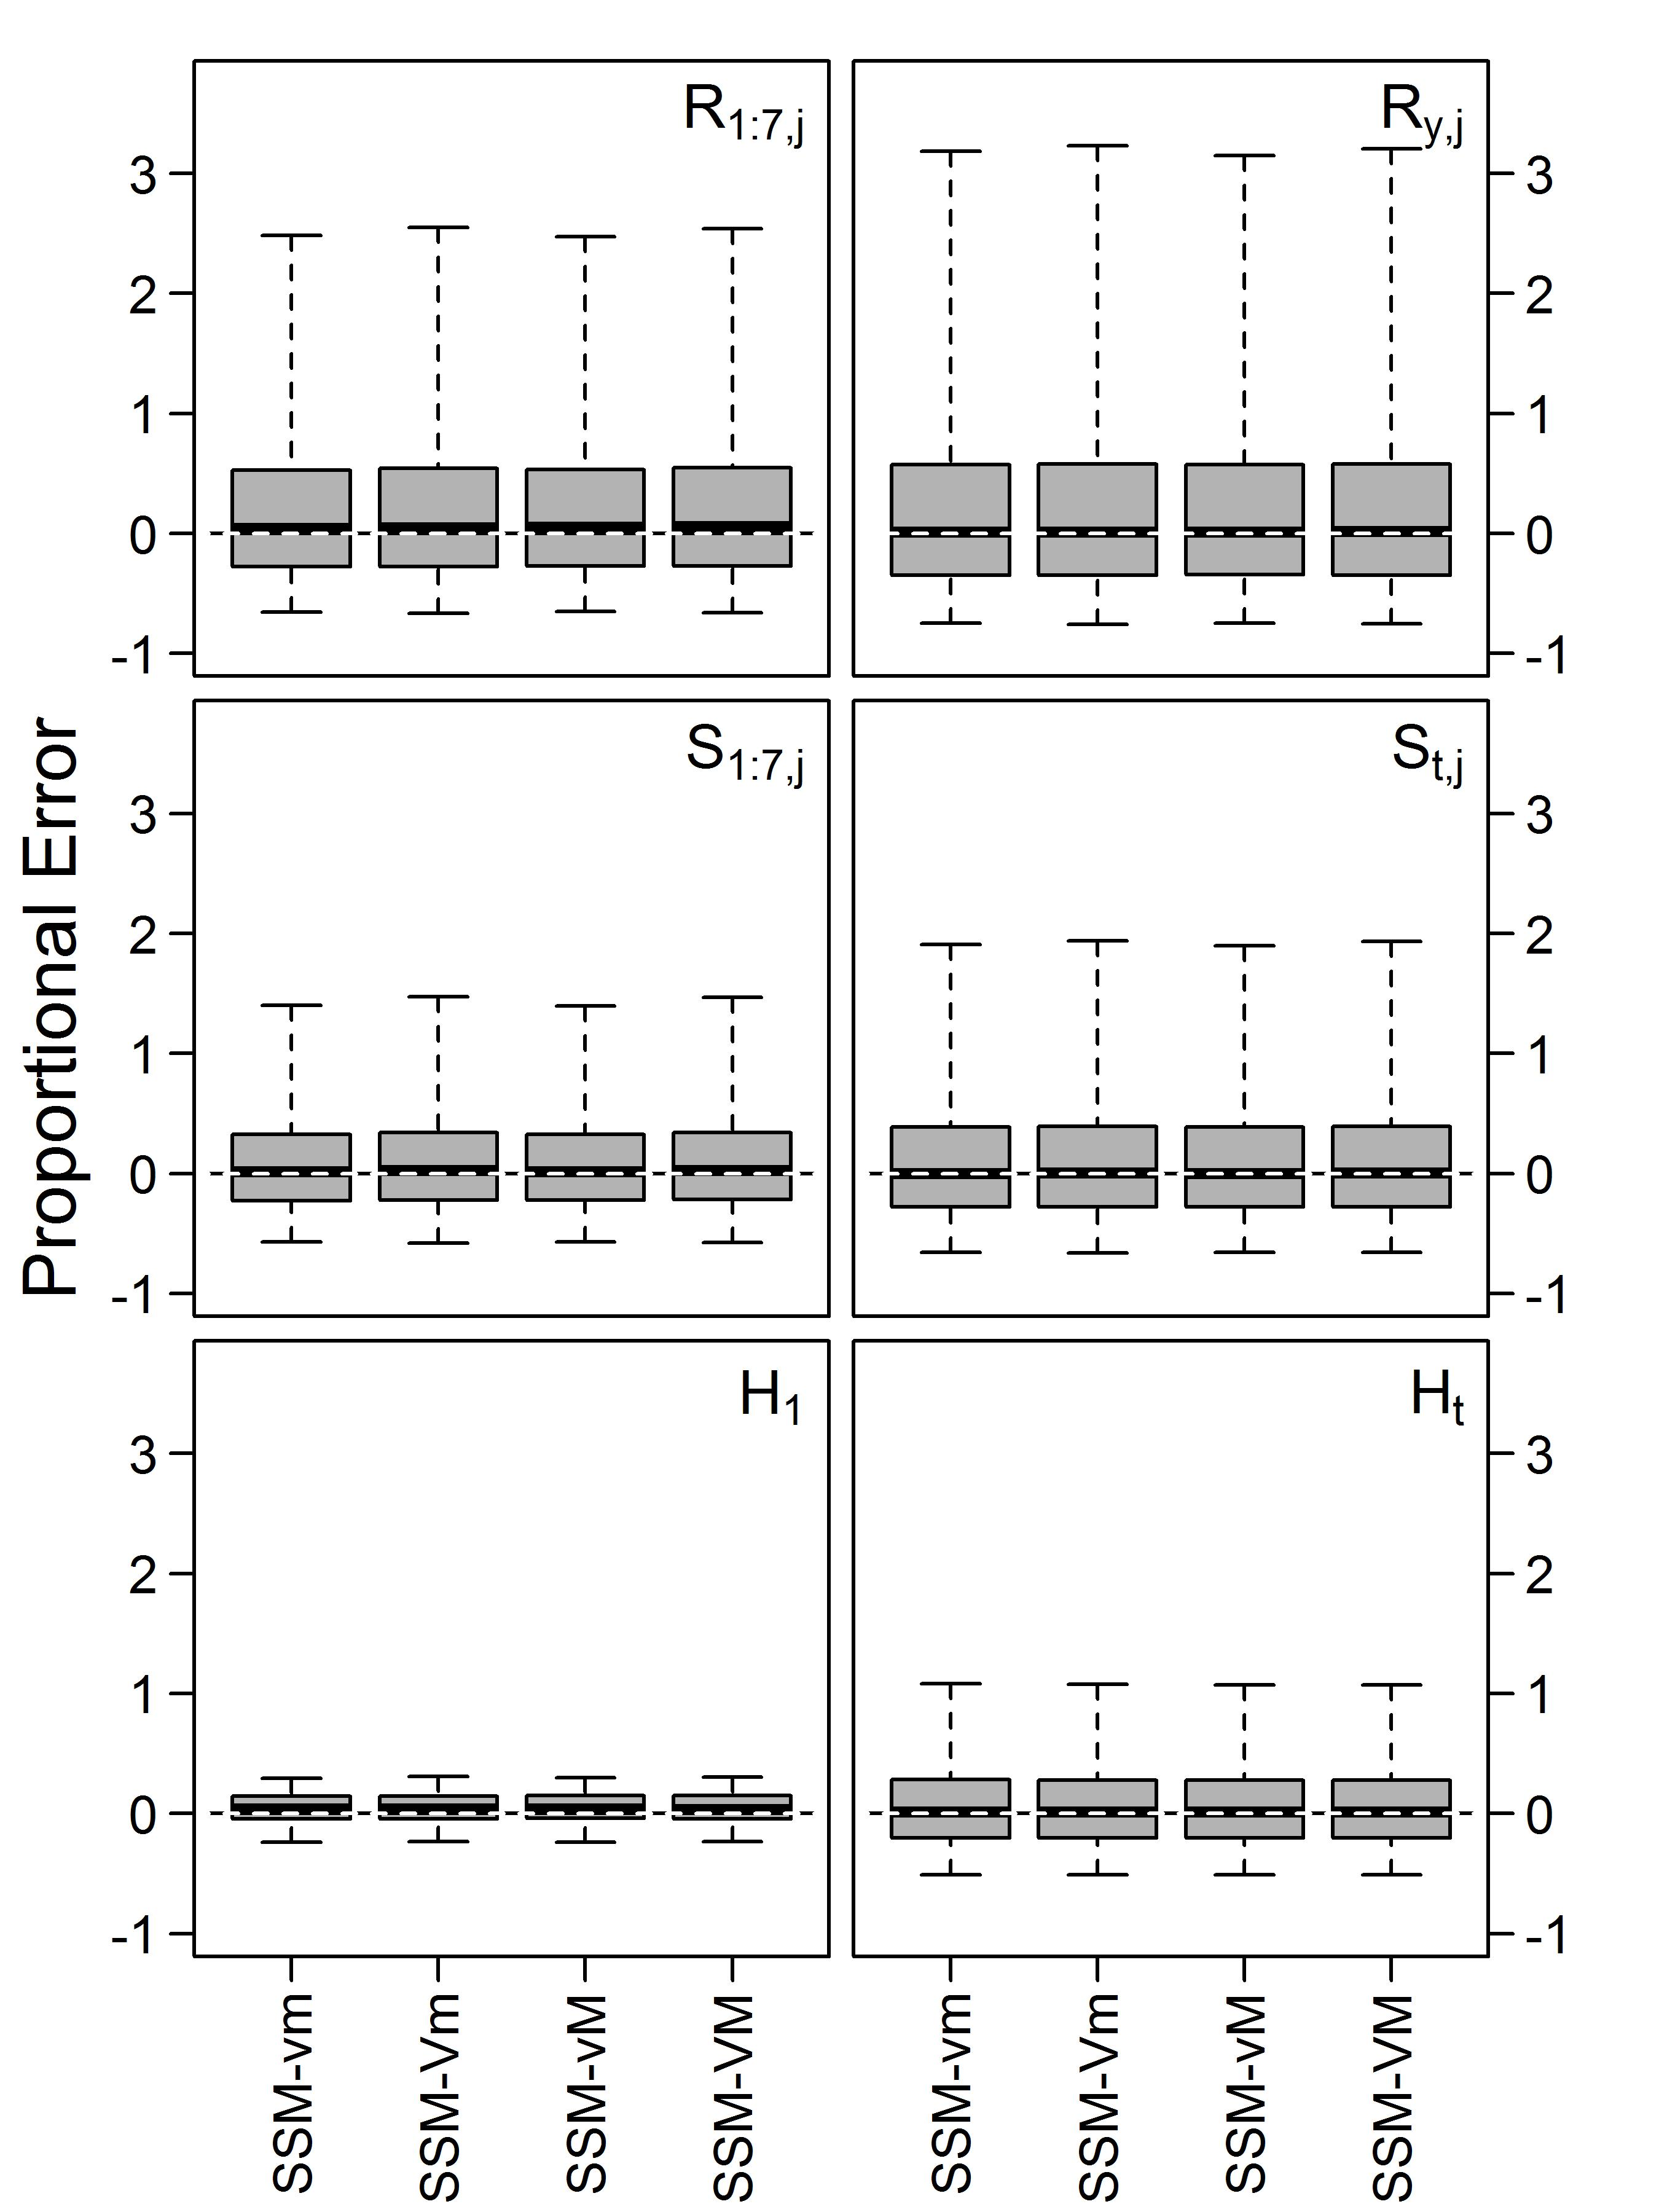
\includegraphics{img/Ch4/state-bias.jpg}
  \caption{Central tendency and variability in proportional error for some abundance states in the multi-stock spawner-recruit models from the simulation-estimation trials. Quantities are separated by the early portion of the time series (left panels) and the entire time series (right panels). Point estimates used were posterior medians.}
  \label{fig:state-bias}
\end{figure}

\clearpage

\begin{figure}
  \centering
  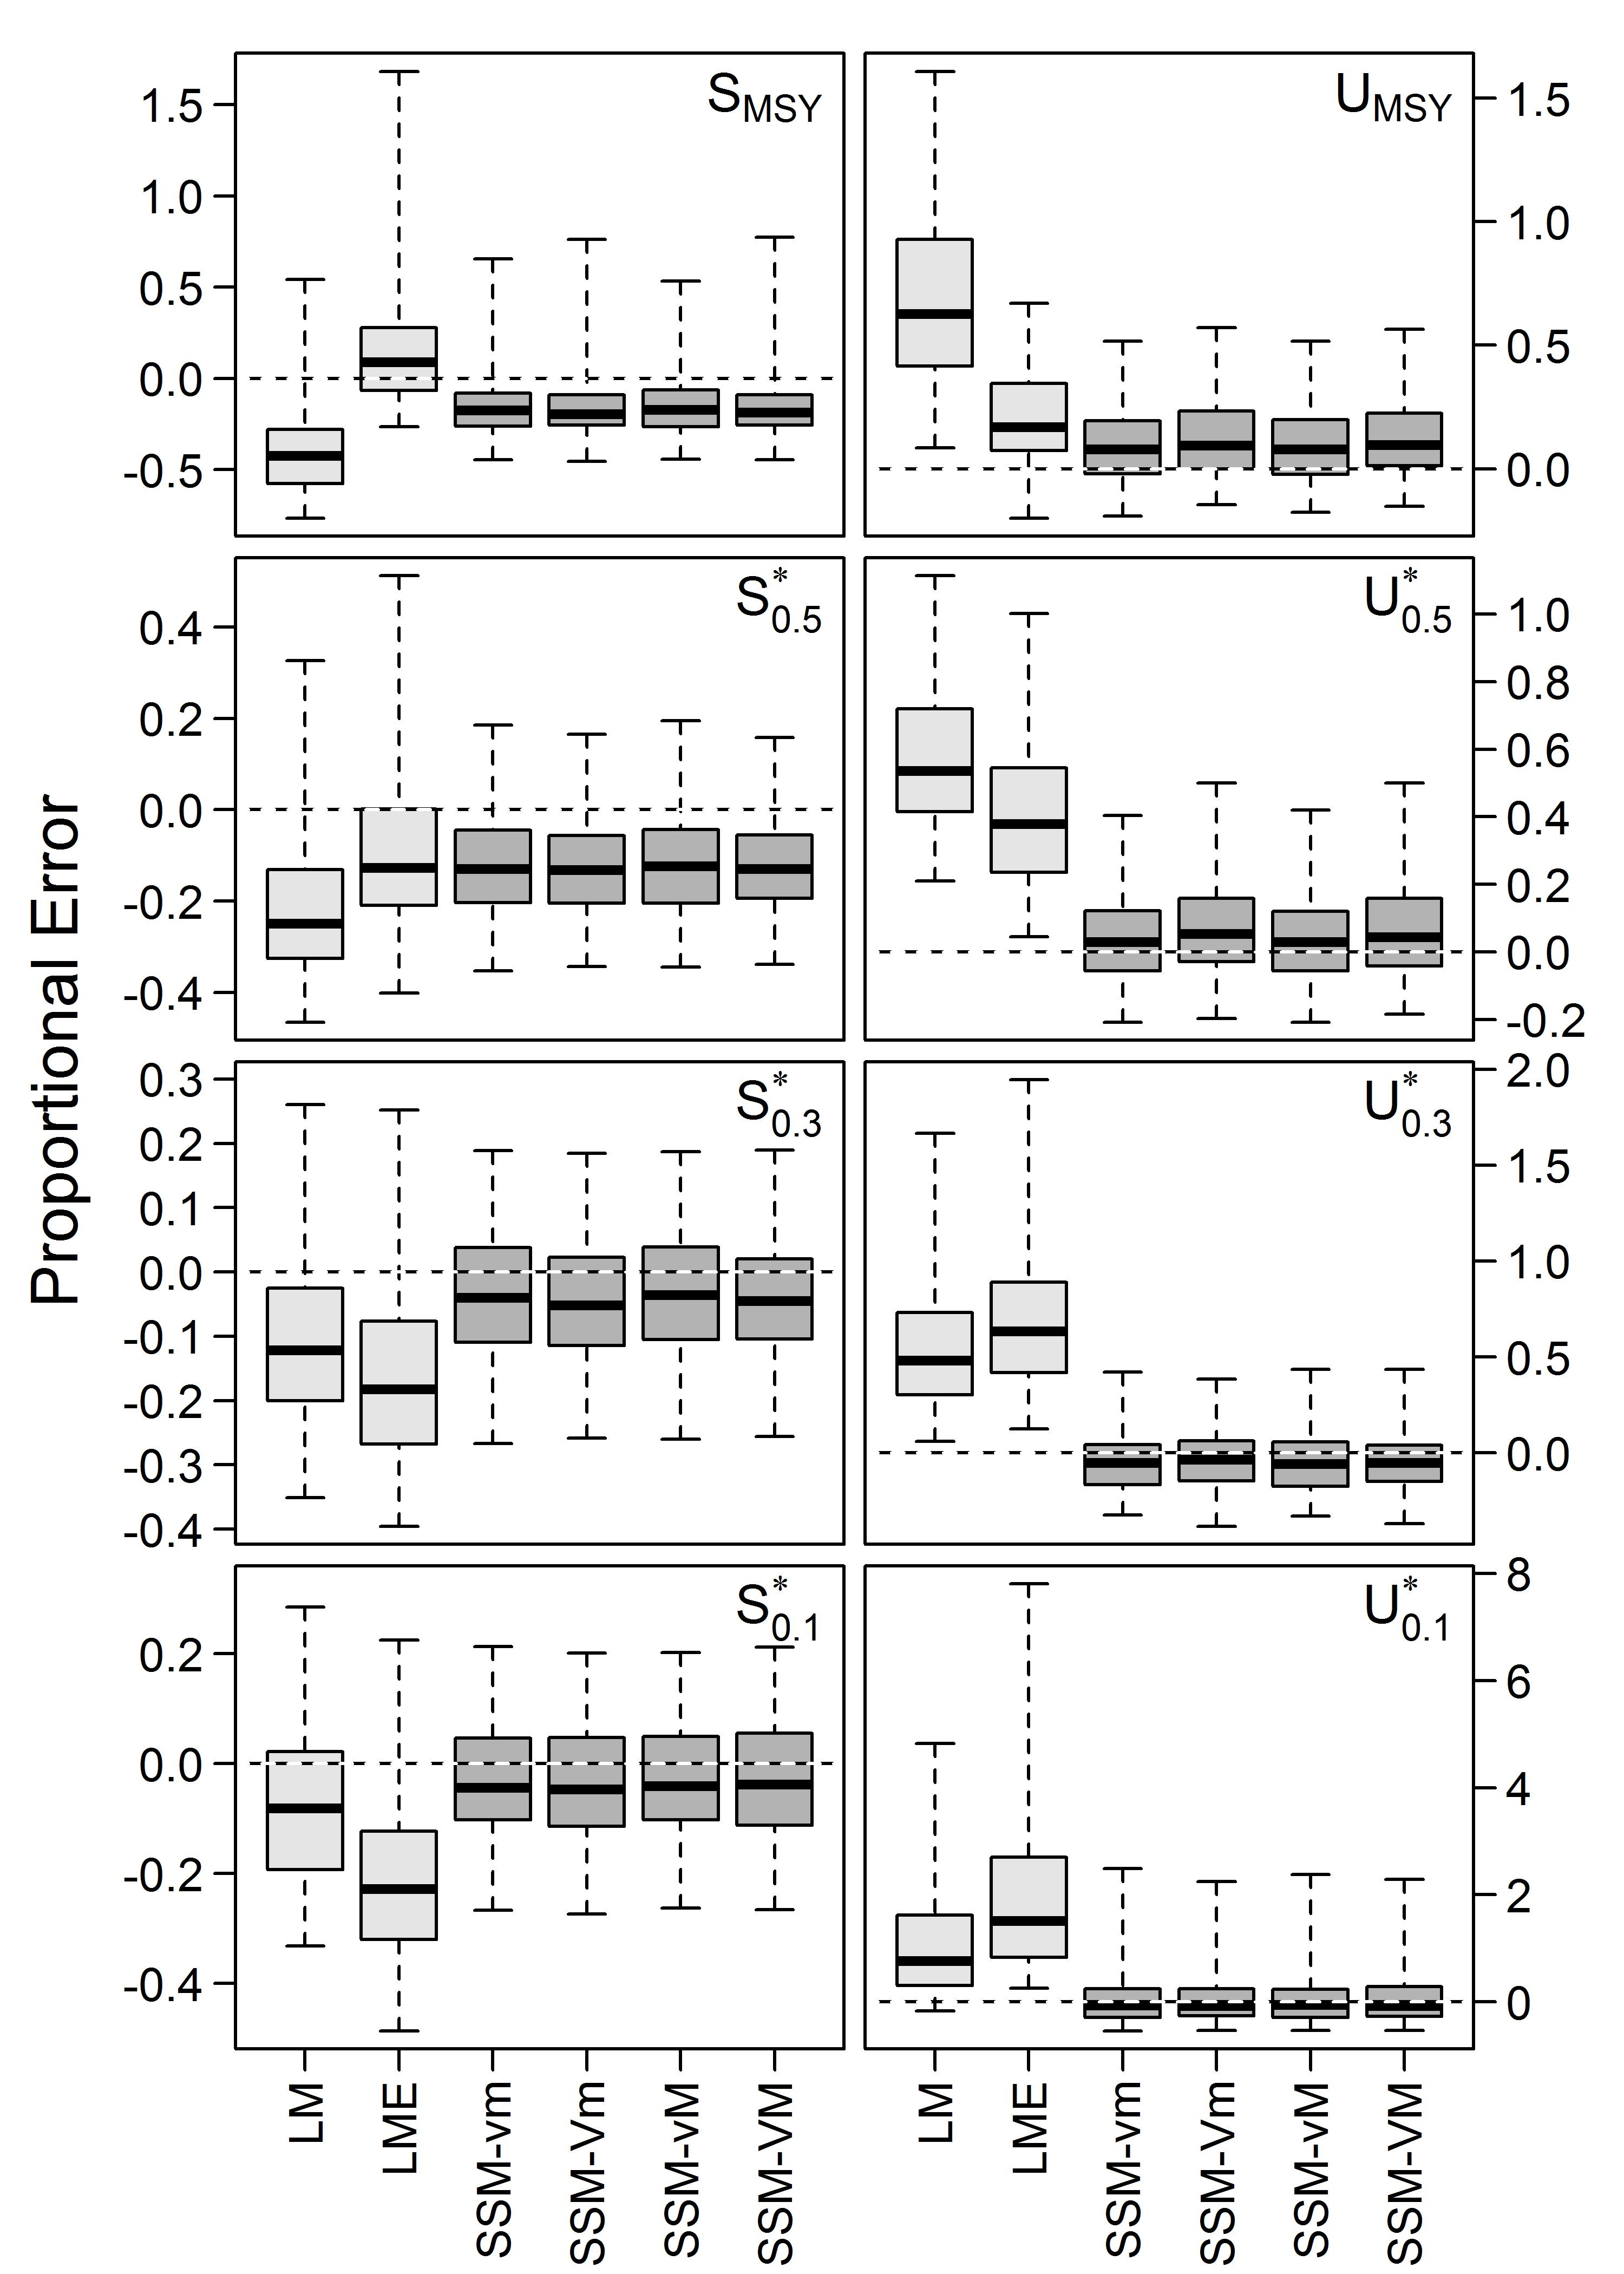
\includegraphics{img/Ch4/ref-point-bias.jpg}
  \caption{Central tendency and variability in proportional error for key biological reference points of the aggregate mixed stock. $S^*_p$ and $U^*_p$ are the aggregate escapement and fully-vulnerable exploitation rate that would ensure no more than $p \cdot 100\%$ of substocks are overfished, respectively. Point estimates used were posterior medians.}
  \label{fig:ref-point-bias}
\end{figure}

\doublespacing

\chapter{Conclusions}\label{ch5}

\noindent
In writing this dissertation, I sought to develop, evaluate, and
illustrate quantitative tools that may be used to address challenges in
salmon management, with particular focus on stocks in western Alaska.
Specifically, the tools sought to reduce uncertainty in decision-making
(in the case of the run timing forecast in Chapter \ref{ch2}) and inform
policy analyses by identifying and measuring the shape and magnitude of
trade-offs between competing objectives (for in-season management in
Chapter \ref{ch3} and long-term management in Chapter \ref{ch4}). In a
broad sense, I believe I have accomplished this objective. The work
presented in this dissertation provides a detailed look at ways
quantitative tools can be used in the management of salmon fisheries in
western Alaska -- some were novel to salmon management, all were novel
with respect to the Kuskokwim River. This final chapter serves as my
reflection on my doctoral work, including further insights on each of
the three primary research projects I completed as well as my time
working in Kuskokwim River management system at the Yukon Delta National
Wildlife Refuge during the summers of 2016 -- 2018.

\section{Further insights on each
project}\label{further-insights-on-each-project}

\subsection{Chapter 2: Run timing
forecasts}\label{chapter-2-run-timing-forecasts}

\noindent
My work on developing run timing forecasts for Kuskokwim River Chinook
salmon has not proven as fruitful as I would have hoped. In each year
since its inception following the 2016 season, the forecast model did
not provide good forecasts of \(D_{50}\): both 2017 and 2018 were
moderately late runs yet the forecast model suggested the runs would be
several days early. Furthermore, a subsequent analysis
\citep{staton-catalano-2019} strongly suggested that using the forecast
model provides no utility for improving perceptions of run size based on
test fishery data. The cause for this finding is two-fold. First,
although the environmental relationships were present for all evaluated
variables (Figure \ref{fig:relationships}; Table \ref{tab:coefs-table}),
the residual variability was too high to result in accurate and precise
forecasts based on them. Second, inter-annual variability in the Bethel
Test Fishery catchability \citep[i.e., the fraction of total run
captured; the inverse is commonly referred to as
``run-per-index'';][]{flynn-hilborn-2004} is the dominant cause of
uncertainty in using this index for predicting run size for much of the
season, not run timing. \citet{staton-catalano-2019} illustrated that
the average CV of abundance predictions from a relationship between
historical abundance and cumulative catch-per-effort each day was
approximately 38\% early in the season and 30\% at the end of the season
(Figure 4 therein). So even after the test fishery is done catching
Chinook salmon, a large amount of uncertainty still remains in the
actual run size (this finding was the same for methods that included and
excluded the run timing forecast). Based on the variability of errors
made by these predictions, it seems this level of uncertainty is
appropriate \citep[also shown in Figure 4 of][]{staton-catalano-2019}.
These findings illustrate that the Bethel Test Fishery is a poor index
of run size, and that the run timing forecast did not improve this
situation.

Still, the forecasting framework I developed was a
statistically-rigorous approach to dealing with high-dimensional
variable selection over time and space. To my knowledge, the sliding
climate window algorithm I employed has not widely been used in
ecological problems. This must either be due to the computational costs
or because it is not well-known, given it is an intuitive and objective
approach to select temporal periods for prediction. After giving a talk
on the forecasting approach I developed, a prominent ecologist in my
field asked whether I thought this constituted a ``data dredge''
analysis, with the implication that it was a bad thing if so. In my
view, data dredging is the practice of searching for all possible
relationships that significantly support some hypothesis and discarding
those that do not, or otherwise developing and confirming ad-hoc
hypotheses based on such a search. First, the notion of statistical
significance was never used in my analysis: all decisions were made
based on actual out-of-sample predictive performance (through forecast
cross-validation) or an index of predictive performance (Akaike's
Information Criterion). Second, no biological hypotheses were tested in
this analysis. Instead, the search was conducted to find the variables
most appropriate for forecasting run timing. In these cases, I think it
is completely rational to perform as exhaustive of a search as possible,
and the approach I developed served as an intuitive and objective means
to do this.

It has been brought to my attention that methods exist that may provide
better forecasts than the approach I used, which was simple/multiple
regression at its core. Specifically, machine learning tools like random
forests could show promise. Additionally, upon further reflection it is
possible that having a continuous forecast of \(D_{50}\) could be less
useful than a discrete forecast of an early, average, or late run. Such
a forecast could be obtained using a multinomial logistic regression
\citep[Ch. 7]{agresti-2002}, which would provide predicted probabilities
that the run will be early, average, or late. In my experience,
uncertainty is more appropriately interpreted by managers when presented
as the probability of outcomes rather than using uncertainty intervals.
There would surely be some loss of resolution (e.g., not all early runs
are equally so), but the categories could be selected based on how the
\(D_{50}\) within each would influence the management inference. For
example, there should exist some thresholds of early/late timing that
would drastically change the inference from if it was an average run; I
would propose that these thresholds be used to delineate the categories.

\subsection{Chapter 3: In-season MSE
analyses}\label{chapter-3-in-season-mse-analyses}

\noindent
In this stochastic MSE analysis of a large salmon-producing river system
in western Alaska, I found several important implications, some that
were known \emph{a priori} and some that were not. For example, the
finding that more conservative substrategies should be favored in small
runs as opposed to large runs makes intuitive sense. However, the
finding that management performance was generally most sensitive to run
timing in large runs rather than small runs was not necessarily known
\emph{a priori}, nor was the finding that good performance can be
attained with a wide range of management strategies. This analysis was
useful in that it provided an objective basis for strategy comparisons
and necessitated critical thinking about the important drivers of system
dynamics (e.g., effort responses to fishery conditions) as well as the
direct ways in which information influences a particular decision. It is
my hope that when presented to fisheries managers and stakeholders in
the region, perhaps a more-informed dialog may be had regarding the
merits and detriments of candidate management strategies.

The most complex assessed management strategy (Strategy \#4; explicit
harvest target, selected probabilistically, updated with in-season
information) is a computer-based representation of the strategy
implemented by the U.S. Fish and Wildlife and the Kuskokwim River
Inter-Tribal Fisheries Commission for the portion of the fishery within
the Yukon Delta National Wildlife Refuge in the years 2015 -- 2018. Each
year has differed in the method and rigor used to (1) initially select
the season-wide harvest target (\(H_T\)), (2) utilize in-season
information to update \(H_T\) and the weekly target (\(H_{T,w}\)), and
(3) determine how much fishing opportunity should be allowed conditional
on \(H_{T,w}\). The overarching structure (e.g., the use of \(H_T\)
based on an escapement limit threshold; \(S_L\)), however, is the same
as the simulated strategy and the probabilistic selection of \(H_T\)
based on risk tolerance (\(P^*\)) and \(S_L\) was conducted for the
first time in 2018.

With the current amount of information available for in-season
management, this is among the most complex management strategies that
could be used for the Kuskokwim Chinook salmon harvest control
situation, and a key finding of the MSE analysis was that it did not
perform overwhelmingly better than far simpler strategies. In the very
smallest runs (50,000 -- 80,000), it did provide substantially better
escapement performance than other policies, but only because the fishery
was all but shut down completely. If this is desirable, the schedules
used by Strategies \#2 and \#3 (Figure \ref{fig:ms2-schedules}) could be
altered to be more conservative for forecasts falling in this bin.
Additionally, uncertainty in the forecast could be included by weighting
schedules by the probability that the run will be in each run size bin
according to the pre-season forecast. In the next smallest category
(80,000 -- 130,000), the gains in escapement utility by using Strategy
\#4 were negligible in comparison to other simpler strategies, and came
at the cost of reducing the harvest utility by approximately half
(Figure \ref{fig:btwn-ms-utilities}). Likewise, it showed no real gains
in harvest equity or even substock exploitation utilities, though no
assessed strategies strongly influenced these metrics. As a result of
these findings, simple schedule-based strategies based solely on a
pre-season forecast (as in Strategy \#2) or combined with in-river
species composition (as in Strategy \#3) would perform well in the
Kuskokwim and similar systems. Given the finding that many strategies
perform similarly, however, perhaps the more important question now
becomes which strategy could meet other objectives not included in this
analysis (e.g., fishers' desire to know when to expect fishing
opportunities far in advance, desire to fish early in the season, etc.)
and is transparent to the parties involved.

\subsection{Chapter 4: Multi-stock spawner-recruit
analyses}\label{chapter-4-multi-stock-spawner-recruit-analyses}

\noindent
For my last project, I evaluated spawner-recruit methods for mixed-stock
salmon fisheries. I developed a novel state-space framework for
simultaneously estimating spawner-recruit parameters from the substocks
within a larger drainage basin when they are all harvested as a
mixed-stock -- the method was shown to perform substantially better than
simpler regression-based approaches that, though they have long been
known for their problems
\citep{ludwig-walters-1981, walters-1985, walters-martell-2004}, they
are still applied to estimate salmon population dynamics parameters and
to provide management recommendations
\citep{clark-etal-2009, korman-english-2013}.

An alternative assessment approach would be to attempt to fit separate
state-space models to the individual substocks as opposed to the more
integrated approach I developed. This approach should retain the
benefits of (1) not needing to exclude some observations because they do
not constitute fully observed brood year pairs and (2) separately
modeling the population dynamics and observation processes to (at least
partially) handle the time-series and errors-in-variables biases.
However, given that not all substock have age composition data, the
individual models would require auxiliary information that was never
observed for that substock and the degree of synchrony between subtocks
would only be available as part of an ad-hoc analysis of patterns from
individual substocks. The more integrated state-space approach I took
did not require such auxiliary age-composition data: only substocks with
observed data were fitted for age composition, and they informed the
maturity model parameters to be used for other substocks. Additionally,
by incorporating a covariance matrix for recruitment variability, the
degree of synchrony in substock dynamics could be informed by years with
data on multiple data on substocks, which could be then used to inform
the latent recruitment states in cases where there were fewer
observations to inform them. Further, as computationally-intensive as
the model I developed was, this approach would be even more so given
independent MCMC sampling would need to be conducted for each substock,
which is a primary reason why it was not evaluated here.

Although the state-space model was applied only to the Kuskokwim River
data and the simulation was designed to mimic the data collection and
substock heterogeneity for that system, the model potentially has wide
applicability to other systems. Many salmon populations are harvested in
mixed stocks; good examples include: the Columbia River in the
northwestern contiguous United States, the Fraser and Skeena River
drainages in British Columbia, Canada, the Bristol Bay stocks in
southwestern Alaska, and the Yukon River in western Alaska and Canada.
All of these systems are composed of several distinct spawning units,
some portion of the harvest occurs as a mixed-stock, and should have
data time series at least as rich as the Kuskokwim River Chinook salmon
data set I used. Granted, in some situations modifications would be
necessary for each specific case. For example, in the Bristol Bay
fishery for sockeye salmon, some harvest occurs by ``intercept fleets'',
where fishers in one district may also harvest fish from other stocks
that are migrating through that area but some harvest also occurs
in-river. This kind of situation would require more detailed information
harvest separated by mixed- and non-mixed sources, but I believe this
would be within the abilites of the state-space model given the data are
available.

\section{Reflections on working for
USFWS}\label{reflections-on-working-for-usfws}

\noindent
In 2016 -- 2018, I took on a more-involved role in the management of
Kuskokwim River salmon fisheries by working as a Pathways
Student\footnote{Unofficial title: Quantitative Ecologist} with the U.S.
Fish at Wildlife Service at the Yukon Delta National Wildlife Refuge
based out of Bethel. Between May and August of these years, I abandoned
my graduate work\footnote{And my loving and understanding girlfriend (as
  of 2016), fiancé (as of 2017), and wife (as of 2018)} and focused on
in-season salmon assessment. In this role, I lead several efforts
dealing with providing information to managers: (1) compiling,
analyzing, and presenting run assessment information in consistent
formats\footnote{Referred to as the ``Daily Assessment Updates'', over
  250 documents were produced using \texttt{\{rmarkdown\}}; examples
  available upon request.}, (2) developing and applying
statistically-rigorous approaches to estimating harvest and effort
arising from short-duration block-openers\footnote{Documented in
  \citet{staton-coggins-2016}, \citet{staton-coggins-2017},
  \citet{staton-2018}, plus a synthesis manuscript currently in
  preparation} and presenting this information to managers, and (3)
presenting risk assessments of seeing undesirable escapement outcomes
conditional on different harvest levels\footnote{2018 only; with the aid
  of a Shiny application I wrote, which has become commonly known as the
  ``\(P^*\) model'' (\url{https://bstaton.shinyapps.io/BayesTool/}).}. I
have enjoyed this role enormously, and it was highly rewarding to apply
my quantitative skills to real world applied management problems, and to
see the inferences be used in decision-making. Though there was a
distinct boundary between the topics I worked on in-season in this role
and my more academic work (i.e., presented in Chapters \ref{ch2},
\ref{ch3}, \ref{ch4} herein), I certainly used what I learned in each
aspect to inform the other. I have no doubt my summers spent in Bethel
resulted in better dissertation research, particularly with respect to
developing the operating model and candidate management strategies used
in Chapter \ref{ch4}, and that I would have been less valuable to the
management system without the quantitative training I have received in
my graduate program.

\setlength{\parskip}{6pt plus 2pt minus 1pt}

\appendix


\captionsetup[figure]{list=yes} \captionsetup[table]{list=yes}

\chapter{Parameterization of the Operating Model in Chapter
\ref{ch3}}\label{appendix-a}

\noindent
There were two main components of the operating model that needed to be
parameterized based on observed information for it to adequately
represent the dynamics of the real Kuskokwim River subsistence salmon
fishery: biological (abundance, timing, spatial characteristics of the
salmon populations, etc.) and sociological (spatial distribution of
effort and desired/needed harvest and temporal aspects of the effort
dynamics). This appendix describes how empirical information collected
in the Kuskokwim River drainage was used to parameterize the operating
model used in the Chapter \ref{ch3} analysis.

\section{Biological quantities}\label{biological-quantities}

\subsection{Chinook salmon total abundance}\label{mse-data-N}

\noindent
Drainage-wide total Chinook salmon run abundance was informed by
\citet{liller-etal-2018}, which reported estimates in the years 1976 --
2017 from a maximum likelihood run reconstruction model. The model was
fitted to 20 escapement indices, commercial fishery
catch-per-unit-effort, and nine years of drainage-wide estimates of
total abundance obtained \emph{via} large-scale mark-recapture
experiments. Based on \citet{liller-etal-2018}, drainage-wide Chinook
salmon abundance has varied between 79,238 (in 2012) and 411,724 (in
1994), with a mean of 216,929 and standard deviation of 87,556. A kernel
density estimator was fitted to this distribution, and the cumulative
density function was obtained to allow sampling of continuous run sizes
in accordance with the historical frequency of run sizes (Figure
\ref{fig:N-plot}). The distribution was truncated at the smallest and
largest runs on record as of 2017 \(\pm\) 30,000 fish.

\subsection{Chinook salmon substock composition}\label{mse-data-pi}

\noindent
Substock composition, or the fraction of the aggregate Chinook salmon
run that was made up of fish from each substock, was informed by the
proportions of telemetry fish that spawned in each region in the years
2015 and 2016 \citep{smith-liller-2017a, smith-liller-2017b}. Although
telemetry data from 2003 -- 2007 were also available, only these years
were used because: (1) they allowed the incorporation of information
from lower river fish (as a result of the tagging location; see Section
\ref{mse-data-ss-timing}) and (2) the management of the fishery resulted
in less selection of upper river substocks in the harvest because
fishing was pushed later in the season than in the 2003 -- 2007 block of
years.

\noindent
In each run of the operating model, a random Dirichlet vector was drawn
with parameter vector equal to {[}lower = 19, middle = 61, upper =
20{]}, which results in an expectation roughly equal to the average
contribution in 2015 and 2016. The use of a Dirichlet distribution with
these parameters generated a modest amount of variability around the
expected substock composition.

\subsection{Chinook salmon run timing}\label{chinook-salmon-run-timing}

\subsubsection{Aggregate timing}\label{aggregate-timing}

\noindent
Run timing information for the aggregate Chinook salmon stock was
available from the Bethel Test Fishery \citep{bue-lipka-2016}, which has
produced a daily value of catch-per-unit-effort for each day between
June 1 and August 24 for the years 1984 -- 2018. The estimates of
location (\(D_{50}\)) and inverse scale (\(h\)) of a logistic function
shown in Table \ref{tab:rt-ests-table} were used to quantify the timing
with which the simulated aggregate Chinook salmon stock runs through the
lower river.

\subsubsection{Substock-specific timing}\label{mse-data-ss-timing}

\noindent
The timing of the specific Chinook salmon substocks (i.e., those
spawning in lower, middle, and upper river tributaries) were informed by
radio telemetry studies
\citep{stuby-2007, smith-liller-2017a, smith-liller-2017b}. The tag date
and final tributary of each fish was available for the years 2003 --
2007 and 2015 -- 2016. In the first block of years, the tagging site was
located near Kalskag, which excluded any fish spawning in lower river
tributaries. In the second block of years, the tag site was moved near
the Johnson River, which allowed the inclusion of fish spawning in the
lower river tributaries. Logistic models \eqref{eq:logistic} were fitted
to the data from each substock and year separately to obtain estimates
of the \(D_{50}\) for each substock in each year data were available,
and differences in \(D_{50}\) for the middle river substocks and each of
the other substocks were calculated (Table \ref{tab:d50-devs-table}).
For parameterizing the run timing of middle river substocks, random
values drawn from the aggregate population estimates were used, and
random uniform deviations for the lower river and upper river \(D_{50}\)
were used in accordance with the deviations shown in Table
\ref{tab:d50-devs-table} (i.e., lower river substocks had a \(D_{50}\)
value that was anywhere between 0 and 3 days later than that of the
middle river, and upper river substocks had a value that was between 5
and 10 days earlier than middle river substocks.

\subsection{Spatial distribution of escapement}\label{calc-esc-p}

\noindent
Due to the spatial nature of the operating model, it was important to
capture the behavior of fish becoming invulnerable to harvest by
swimming up a spawning tributary. This aspect was informed using data
from the telemetry studies: it was possible to quantify the fraction of
all tagged fish that made it to a particular reach that ultimately
spawned in a tributary with a confluence in that reach in each year.
These fractions were averaged across years and the average was used to
dictate how many fish from each substock \(s\) in reach \(r\) on day
\(d\) would ``peel off'' from the mainstem into a tributary in that
reach on that day. For the aggregate chum/sockeye stock, which does not
have this kind of information, the substock structure was removed. These
estimates are shown in Table \ref{tab:esc-p-table}.

\subsection{Species ratios}\label{mse-data-ratios}

\noindent
Because chum and sockeye salmon lack the abundance data available for
Chinook salmon, their daily entry dynamics were modeled using observed
species ratios from the Bethel Test Fishery. These data were prepared by
taking the catch-per-unit-effort of chum salmon plus sockeye salmon, and
dividing it by the catch-per-unit-effort of Chinook salmon on each day
of each year for which data were available. This represents how many
vulnerable chum/sockeye salmon were available for harvest relative to
Chinook salmon. Daily values that could not be calculated (i.e., when
zero Chinook salmon were caught) were populated with the average value
for all years for which a species ratio could be calculated on that same
day. These annual time series were highly variable from day to day,
likely as a result of sampling variability, so a cubic spline smoother
was fitted to remove this variability. The time series of smoothed
ratios from all years is shown in Figure \ref{fig:ratios-plot}.

In each simulated year, one randomly sampled annual time series was
selected to generate the daily species composition for that year. To
avoid anomalous outcomes, i.e., unlikely combinations of Chinook run
timing and abundance matched with very high or low species ratios in the
simulation. I investigated two historical variables for covariance with
the species ratio: \(D_{50}\) and total Chinook salmon run size using a
\(\chi^2\) test for independence. For each historical year, run timing,
run size, and the first date at which a species ratio of 15:1 was
observed were categorized into three bins, with endpoints delineated by
the 33\% and 66\% percentiles of each variable. I was interested in
whether Chinook salmon runs with different run timing or size tended to
coincide with attaining high species ratios earlier or later in the
season. If these sorts of patterns were present, they would need to be
accounted for in the simulation.

The first date of 15:1 ratios and Chinook salmon run timing had more
non-independence (\(\chi^2 = 11, df = 4, p = 0.027\)) than Chinook
salmon run size (\(\chi^2 = 1.84, df = 4, p = 0.765\)). This indicated
that species ratios could be drawn independently with regards to the
simulated Chinook salmon run size, but not the simulated run timing. As
shown in Table \ref{tab:ratio-timing-cov-table}, the probability of
having early high ratios has been historically highest in early Chinook
runs. Late Chinook salmon runs tended to occur in years that had later
dates of 15:1. I incorporated these patterns in the simulation by first
sampling the run timing for that simulated year, then assigning it to a
category, then sampling a ratio category with probability equal to the
appropriate column in Table \ref{tab:ratio-timing-cov-table}. Finally, a
year was randomly selected from the approximately 10 years in that same
category, and the daily species ratios that year were used to drive the
species composition time series in that simulated year.

\section{Sociological quantities}\label{sociological-quantities}

\subsection{Needed salmon harvest by river reach}\label{mse-data-needs}

\noindent
The term ``minimally needed salmon harvest'' salmon harvest refers to
the amount of salmon that would satisfy the very basics of the
subsistence needs of fishers in the drainage -- without meeting this
level it is reasonable to assume the fishing population is experiencing
hardship. ``Maximally needed salmon harvest'' represents the salmon
harvest that would completely meet subsistence needs (i.e., if as many
fish could be harvested as desired). The Alaska Board of Fisheries has
produced ranges for each species, termed the ``Amounts Reasonably
Necessary for Subsistence'' (ANS) and represents the drainage-wide range
of harvest by species needed to sustain subsistence fishers each year.
These ANS ranges are 67,200 -- 109,800 for Chinook salmon and 73,400 --
175,100 for chum+sockeye salmon. In this analysis, the lower bound of
the ANS range was used to specify minimally needed salmon harvest by
species, and the upper bound of the range was used to specify maximally
needed salmon harvests. Maximally needed amounts were used to drive the
dynamics of the effort model and the midpoint between the minimal and
maximal needs was used to measure the attainment of management
objectives.

However, these values are only available for the entire drainage -- they
are not partitioned to individual villages. For this analysis, a minimal
and maximal value was needed for the villages located within each reach.
The drainage-wide totals were thus partitioned by calculating the
average fraction that villages in each reach have harvested of the
drainage-wide. \citet{hamazaki-2011} present year-, species- and
village-specific salmon harvests for the period (1990 -- 2009), and data
through 2015 can be found in \citet{carroll-hamazaki-2012},
\citet{shelden-etal-2014}, \citet{shelden-etal-2015},
\citet{shelden-etal-2016a}, and \citet{shelden-etal-2016b}. Only years
1990 -- 2000 were included for the spatial distribution of salmon need
because stakeholders provided input during meetings that indicated the
restrictions in recent years make the harvest proportions
non-representative and that the earlier years are more reflective of how
harvest should be distributed. The partitioned values by species are
shown in Table \ref{tab:socio-spatial-table}.

\subsection{Maximum daily effort by river reach}\label{mse-data-effort}

\noindent
A key aspect of the sociological component to the operating model was
the spatial distribution of maximum fishing effort, i.e., the greatest
number of boat days that can be exerted by villages in each reach when
the fishery is open. This maximum effort was altered as the simulated
salmon season progressed based on the effort response submodel. The
important characteristic to capture is the proportion of all effort that
is attributable to each reach, i.e., the scale is not important as the
efficiency of any one unit can be adjusted by altering the \(q\)
parameter. To determine how effort should be apportioned to each reach,
a simple index of effort for each village and year was devised based on
the number of reported fishing households. The Alaska Department of Fish
and Game has collected this information since 1990, and it is presented
in the same studies that quantified subsistence harvest patterns:
\citet{hamazaki-2011}, \citet{carroll-hamazaki-2012},
\citet{shelden-etal-2014}, \citet{shelden-etal-2015},
\citet{shelden-etal-2016a}, and \citet{shelden-etal-2016b}. The data
were reported as the number of households that ``usually fish'' and the
number of households that ``do not usually fish'' as surveyed each year
(as well as the number of ``unknown'' fishing status households). First,
any unknown households were apportioned to the other two categories by
assuming the information was missing at random: if 60\% of the fishing
households belonged to the ``usually fishes'' category in a village in a
year, then 60\% of the unknown households were apportioned to ``usually
fishes'' and 40\% to ``does not usually fish''. The effort index was
calculated for each village as 1 \(\times\) \# usually + 0.5 \(\times\)
\# not usually, summed the values across villages within each reach and
year, calculated the annual proportion belonging in each reach, and
averaged these values across years.

\clearpage
\singlespacing

\begin{longtable}[t]{>{\bfseries}lcclcclcc}
\caption{\label{tab:d50-devs-table}Difference between $D_{50}$ for tagged fish destined for lower or upper river tributaries and those destined for middle river tributaries. These estimates were used to inform Chinook salmon substock-specific run timing.}\\
\toprule
\textbf{Year} & \textbf{Lower} & \textbf{Upper}\\
\midrule
2003 &  & -2.0\\
2004 &  & -9.5\\
2005 &  & -4.9\\
2006 &  & -7.8\\
2007 &  & -2.5\\
\addlinespace
2015 & -0.7 & -10.7\\
2016 & 2 & -9.8\\
\bottomrule
\end{longtable}

\clearpage

\begin{longtable}[t]{clccccclccccclccccclccccclccccclcccc}
\caption{\label{tab:esc-p-table}Spatial distribution of escapement in the operating model. The number in each cell represents $\psi_{r,s}$: the fraction of fish from a stock that make it to a reach and survive the fishery that ultimately escape and spawn in a tributary with a confluence with the main stem Kuskokwim located in that reach. These estimates were obtained from radio telemetry studies as described in Section \ref{calc-esc-p}, and the chum/sockeye salmon estimates were obtained by removing the substock structure from the Chinook salmon data.}\\
\toprule
\multicolumn{1}{c}{\bfseries } & \multicolumn{1}{c}{\bfseries } & \multicolumn{3}{c}{\bfseries Chinook Salmon} & \multicolumn{1}{c}{\bfseries } \\
\cmidrule(l{2pt}r{2pt}){3-5}
\textbf{Reach \#} & \textbf{Tributaries in Reach} & \textbf{Lower} & \textbf{Middle} & \textbf{Upper} & \textbf{Chum/Sockeye}\\
\midrule
\addlinespace[0.3em]
\multicolumn{36}{l}{\textbf{Lower River}}\\
\hline
\hspace{1em}4 & Kwethluk & 65.3\% & 0\% & 0\% & 12.4\%\\
\hspace{1em}5 & Kasigluk, Kisaralik & 80.1\% & 0\% & 0\% & 6\%\\
\hspace{1em}6 & Tuluksak & 100\% & 0\% & 0\% & 1.7\%\\
\addlinespace[0.3em]
\hline
\multicolumn{36}{l}{\textbf{Middle River}}\\
\hline
\hspace{1em}9 & Aniak & 0\% & 28.1\% & 0\% & 24.6\%\\
\hspace{1em}10 & Owhat & 0\% & 0.5\% & 0\% & 0.4\%\\
\hspace{1em}11 & Holokuk, Sue Creek, Veahna & 0\% & 3.7\% & 0\% & 3.4\%\\
\hspace{1em}12 & Oskawalik & 0\% & 2.7\% & 0\% & 2.4\%\\
\hspace{1em}13 & Crooked Creek, George & 0\% & 6\% & 0\% & 4.8\%\\
\hspace{1em}15 & Vreeland, Holitna & 0\% & 77.3\% & 0\% & 64.6\%\\
\hspace{1em}16 & Stony & 0\% & 32.8\% & 0\% & 25.8\%\\
\hspace{1em}17 & Swift, Tatlawiksuk & 0\% & 100\% & 0\% & 55.9\%\\
\addlinespace[0.3em]
\hline
\multicolumn{36}{l}{\textbf{Upper River}}\\
\hline
\hspace{1em}20 & Selatna, Black & 0\% & 0\% & 6\% & 6\%\\
\hspace{1em}22 & Takotna & 0\% & 0\% & 17.5\% & 17.5\%\\
\hspace{1em}24 & Middle Fork & 0\% & 0\% & 94\% & 94\%\\
\hspace{1em}26 & South Fork, East Fork & 0\% & 0\% & 100\% & 100\%\\
\bottomrule
\end{longtable}

\clearpage

\begin{table}

\caption{\label{tab:ratio-timing-cov-table}Non-independence of historically-observed Chinook salmon run timing and the date at which the species ratio of 15:1 chum+sockeye:Chinook was obtained. Columns sum to 1 and represent the empirical probability of observing a ratio type in each of the three categories along the rows. Independence would have all cells equal to 33.3\% -- note that early high ratios tend to occur in years with early Chinook salmon runs, and \textit{vice versa}.}
\centering
\begin{tabular}[t]{>{\bfseries}lccclccclccclccc}
\toprule
\multicolumn{1}{c}{\bfseries } & \multicolumn{3}{c}{\bfseries Chinook Salmon Run Timing} \\
\cmidrule(l{2pt}r{2pt}){2-4}
\textbf{Ratio Category} & \textbf{Earliest 33\%} & \textbf{Middle 33\%} & \textbf{Latest 33\%}\\
\midrule
Earliest 33\% & 66.7\% & 11.1\% & 20\%\\
Middle 33\% & 33.3\% & 44.4\% & 20\%\\
Latest 33\% & 0\% & 44.4\% & 60\%\\
\bottomrule
\end{tabular}
\end{table}

\clearpage

\begin{landscape}\begin{table}

\caption{\label{tab:socio-spatial-table}Key sociological quantities used in the operating model, broken down by spatial area (reach). Each reach is 35 km in main stem river length. Effort ($E_{\text{MAX},r}$) is expressed as the maximum number of boats fishing per day in reach $r$. The \% columns represent the average fraction of the total harvest by species that was harvested by villages within each reach over the period 1990 -- 2000. Harvest values have been rounded to the nearest 100 for ease of presentation, but the total column represents the sum of non-rounded quantities. Although these data were available through 2015, region stakeholders indicated that the recent years have been contaminated by harvest restrictions, and that these earlier years would be more representative.}
\centering
\begin{tabular}[t]{lllllllll}
\toprule
\multicolumn{1}{c}{\bfseries } & \multicolumn{1}{c}{\bfseries } & \multicolumn{1}{c}{\bfseries } & \multicolumn{3}{c}{\bfseries Chinook Salmon} & \multicolumn{3}{c}{\bfseries Chum/Sockeye Salmon} \\
\cmidrule(l{2pt}r{2pt}){4-6} \cmidrule(l{2pt}r{2pt}){7-9}
\textbf{Reach \#} & \textbf{Villages in Reach} & \textbf{Effort} & \textbf{\%} & \textbf{Min.} & \textbf{Max.} & \textbf{\%} & \textbf{Min.} & \textbf{Max.}\\
\midrule
\addlinespace[0.3em]
\multicolumn{9}{l}{\textbf{Lower River}}\\
\hline
\hspace{1em}1 & Tuntutuliak, Eek & 42 & 7.6\% & 5,100 & 8,300 & 6.2\% & 4,600 & 10,900\\
\hspace{1em}2 & Atmautluak, Kasigluk, Nunapitchuk & 74 & 11\% & 7,400 & 12,000 & 13.6\% & 10,000 & 23,900\\
\hspace{1em}3 & Napakiak, Napaskiak, Oscarville, Bethel & 415 & 40.5\% & 27,200 & 44,500 & 34.1\% & 25,000 & 59,600\\
\hspace{1em}4 & Kwethluk, Akiachak & 74 & 17.2\% & 11,600 & 18,900 & 15.2\% & 11,200 & 26,600\\
\hspace{1em}5 & Akiak & 18 & 4.3\% & 2,900 & 4,800 & 4.9\% & 3,600 & 8,600\\
\hspace{1em}6 & Tuluksak & 21 & 3.9\% & 2,600 & 4,300 & 4.4\% & 3,300 & 7,800\\
\addlinespace[0.3em]
\hline
\multicolumn{9}{l}{\textbf{Middle River}}\\
\hline
\hspace{1em}8 & Lower Kalskag, Upper Kalskag & 33 & 5.1\% & 3,400 & 5,600 & 4.2\% & 3,100 & 7,400\\
\hspace{1em}9 & Aniak & 46 & 4.2\% & 2,800 & 4,600 & 4.6\% & 3,400 & 8,100\\
\hspace{1em}10 & Chuathbaluk & 9 & 1.3\% & 900 & 1,400 & 2.1\% & 1,600 & 3,700\\
\hspace{1em}13 & Crooked Creek & 9 & 1\% & 600 & 1,100 & 1.5\% & 1,100 & 2,600\\
\hspace{1em}14 & Red Devil & 6 & 0.3\% & 200 & 400 & 1.1\% & 800 & 2,000\\
\hspace{1em}15 & Sleetmute & 12 & 1.1\% & 800 & 1,200 & 2.1\% & 1,500 & 3,600\\
\hspace{1em}16 & Lime Village, Stony River & 10 & 0.7\% & 500 & 700 & 4\% & 3,000 & 7,000\\
\addlinespace[0.3em]
\hline
\multicolumn{9}{l}{\textbf{Upper River}}\\
\hline
\hspace{1em}22 & McGrath, Nikolai, Takotna, Telida & 42 & 1.7\% & 1,100 & 1,800 & 1.9\% & 1,400 & 3,300\\
\textbf{\hspace{1em}Total} & \textbf{} & \textbf{800} & \textbf{100\%} & \textbf{67,200} & \textbf{109,800} & \textbf{100\%} & \textbf{73,400} & \textbf{175,100}\\
\bottomrule
\end{tabular}
\end{table}
\end{landscape}

\clearpage

\begin{figure}
  \centering
  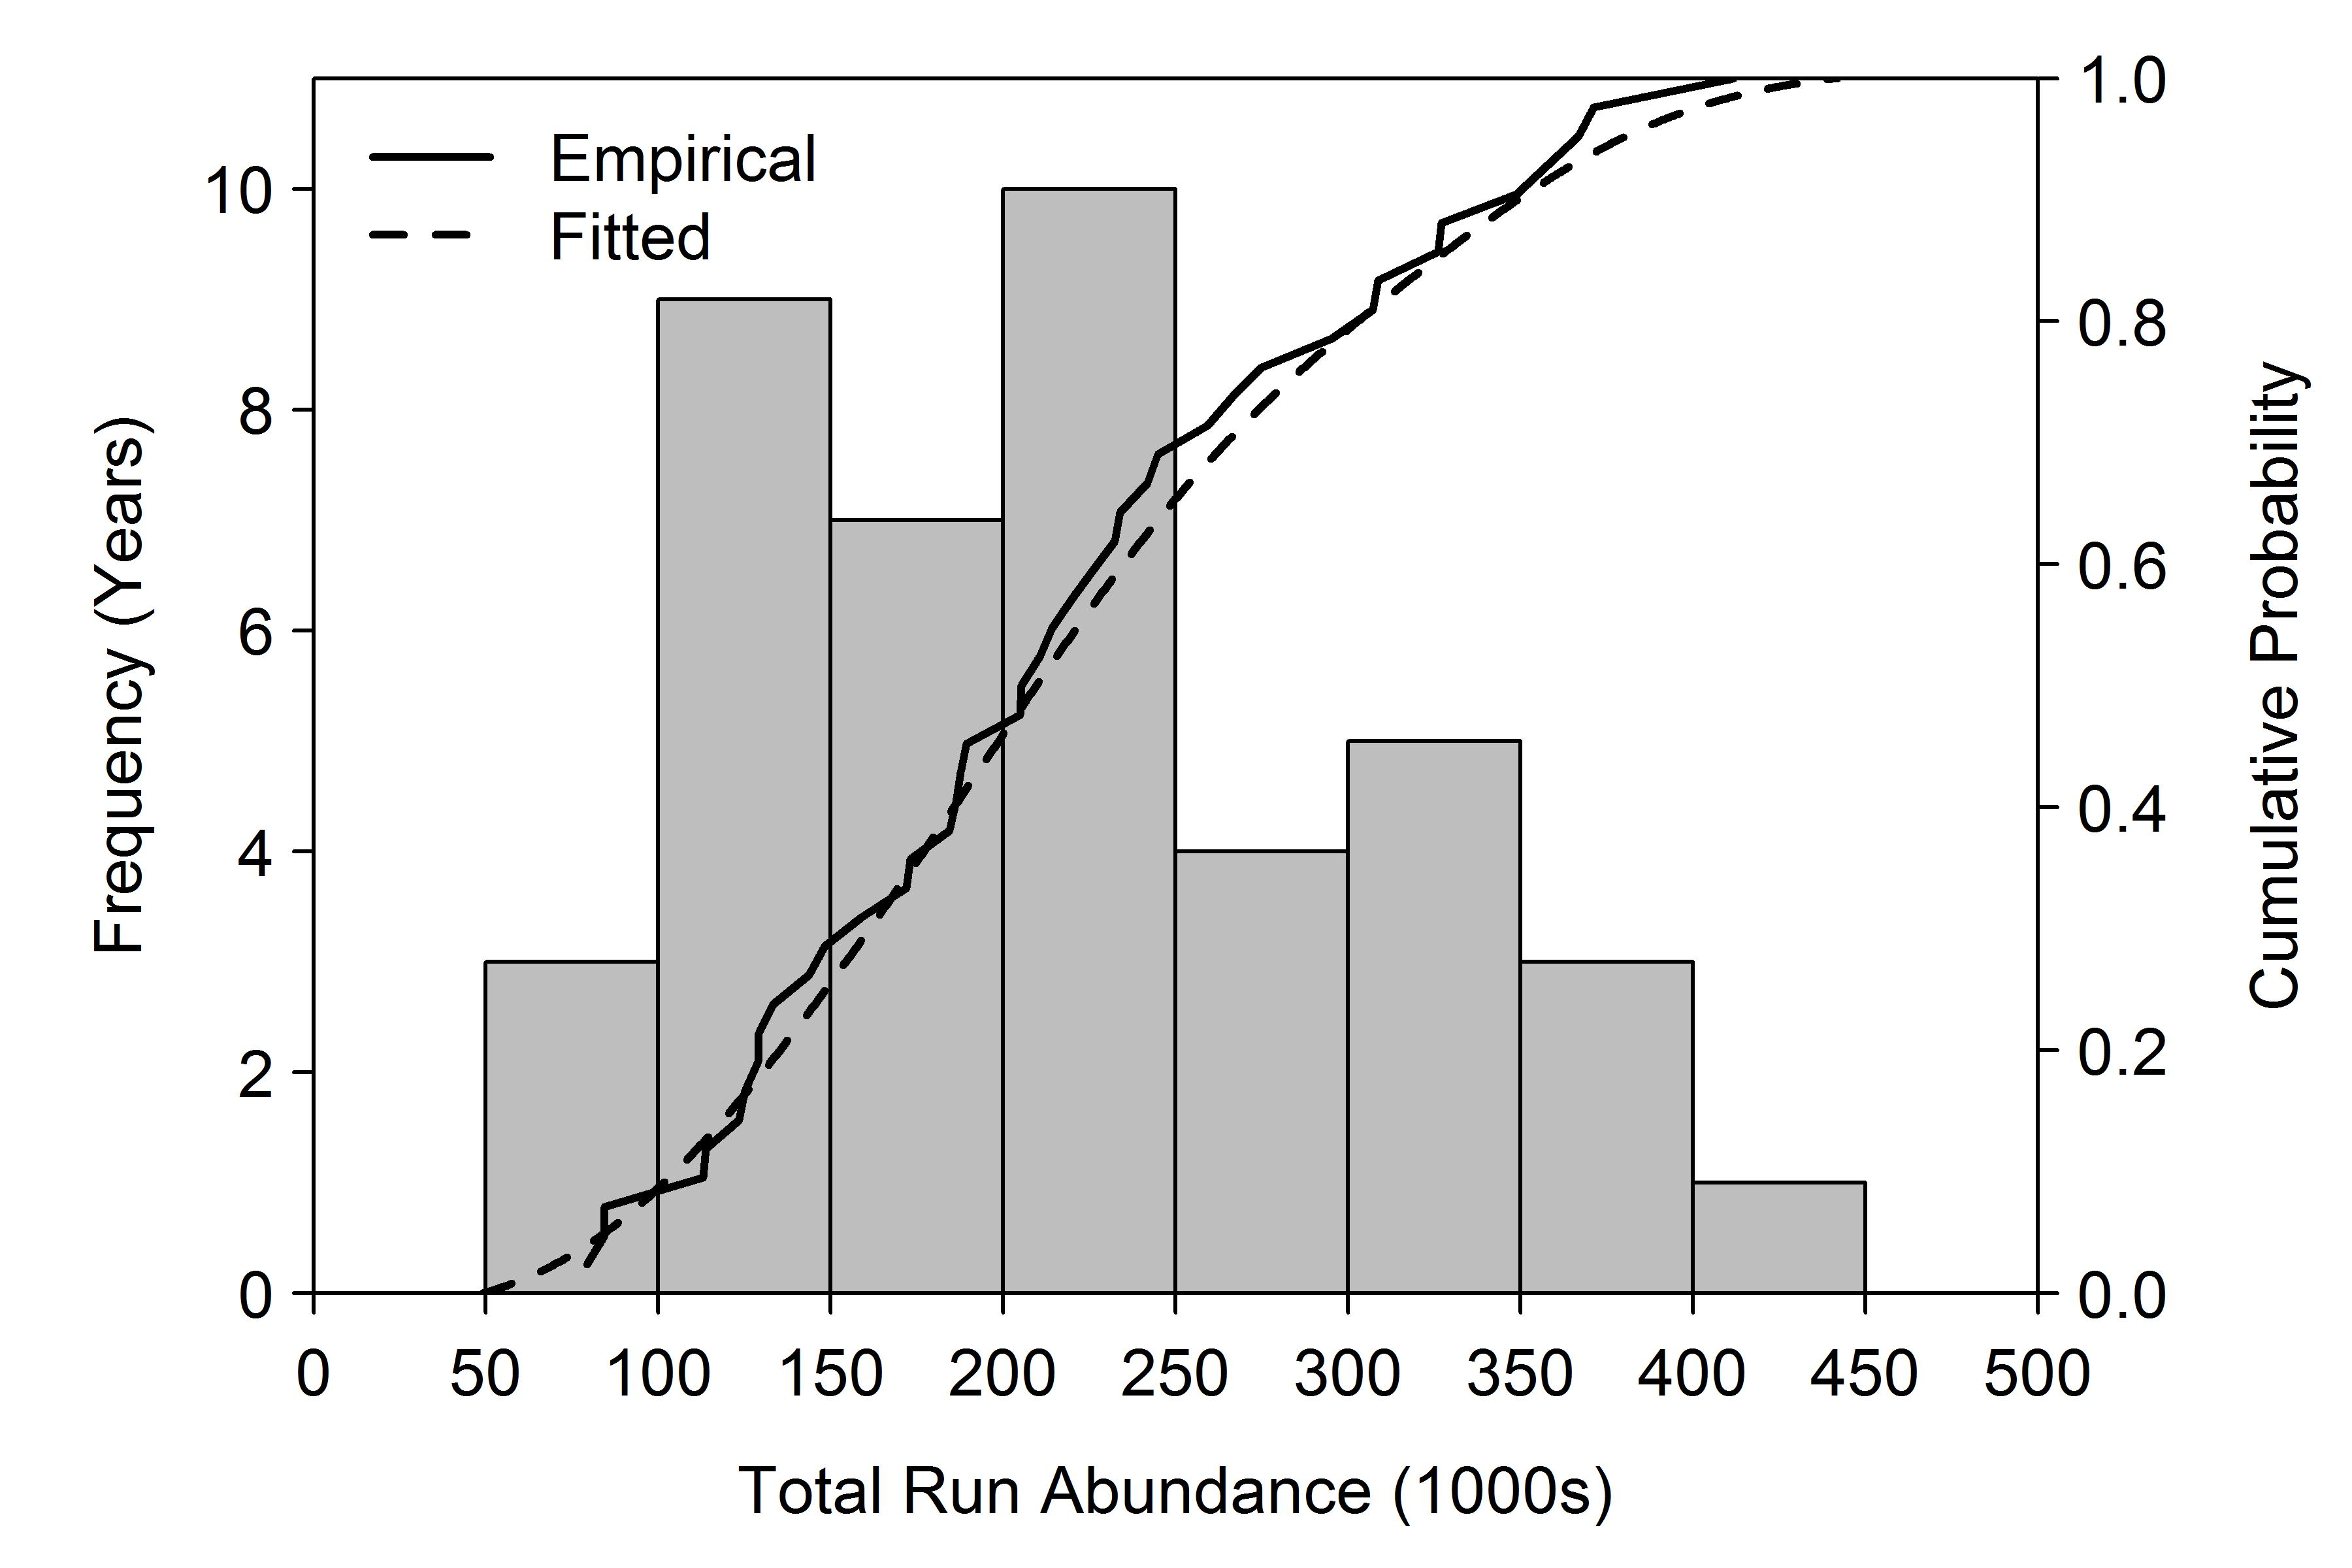
\includegraphics{img/Ch3/N-plot.jpg}
  \caption{Distribution of total drainage-wide run size for Kuskokwim River Chinook salmon, as presented in \cite{liller-etal-2018}. This distribution was used to generate the run size of the aggregate Chinook salmon populations entering the fishery system in a simulated year. The secondary $y$-axis represents the probability of a run falling below a given run size according to the historical frequency of run sizes; where the solid line shows the empirical cumulative distribution function and the dashed line shows one obtained by fitting a kernel density smoother to the empirical data. The fitted distribution was used for simulation to prevent the same 42 run size values from being replicated in the analysis.}
  \label{fig:N-plot}
\end{figure}

\clearpage

\begin{figure}
  \centering
  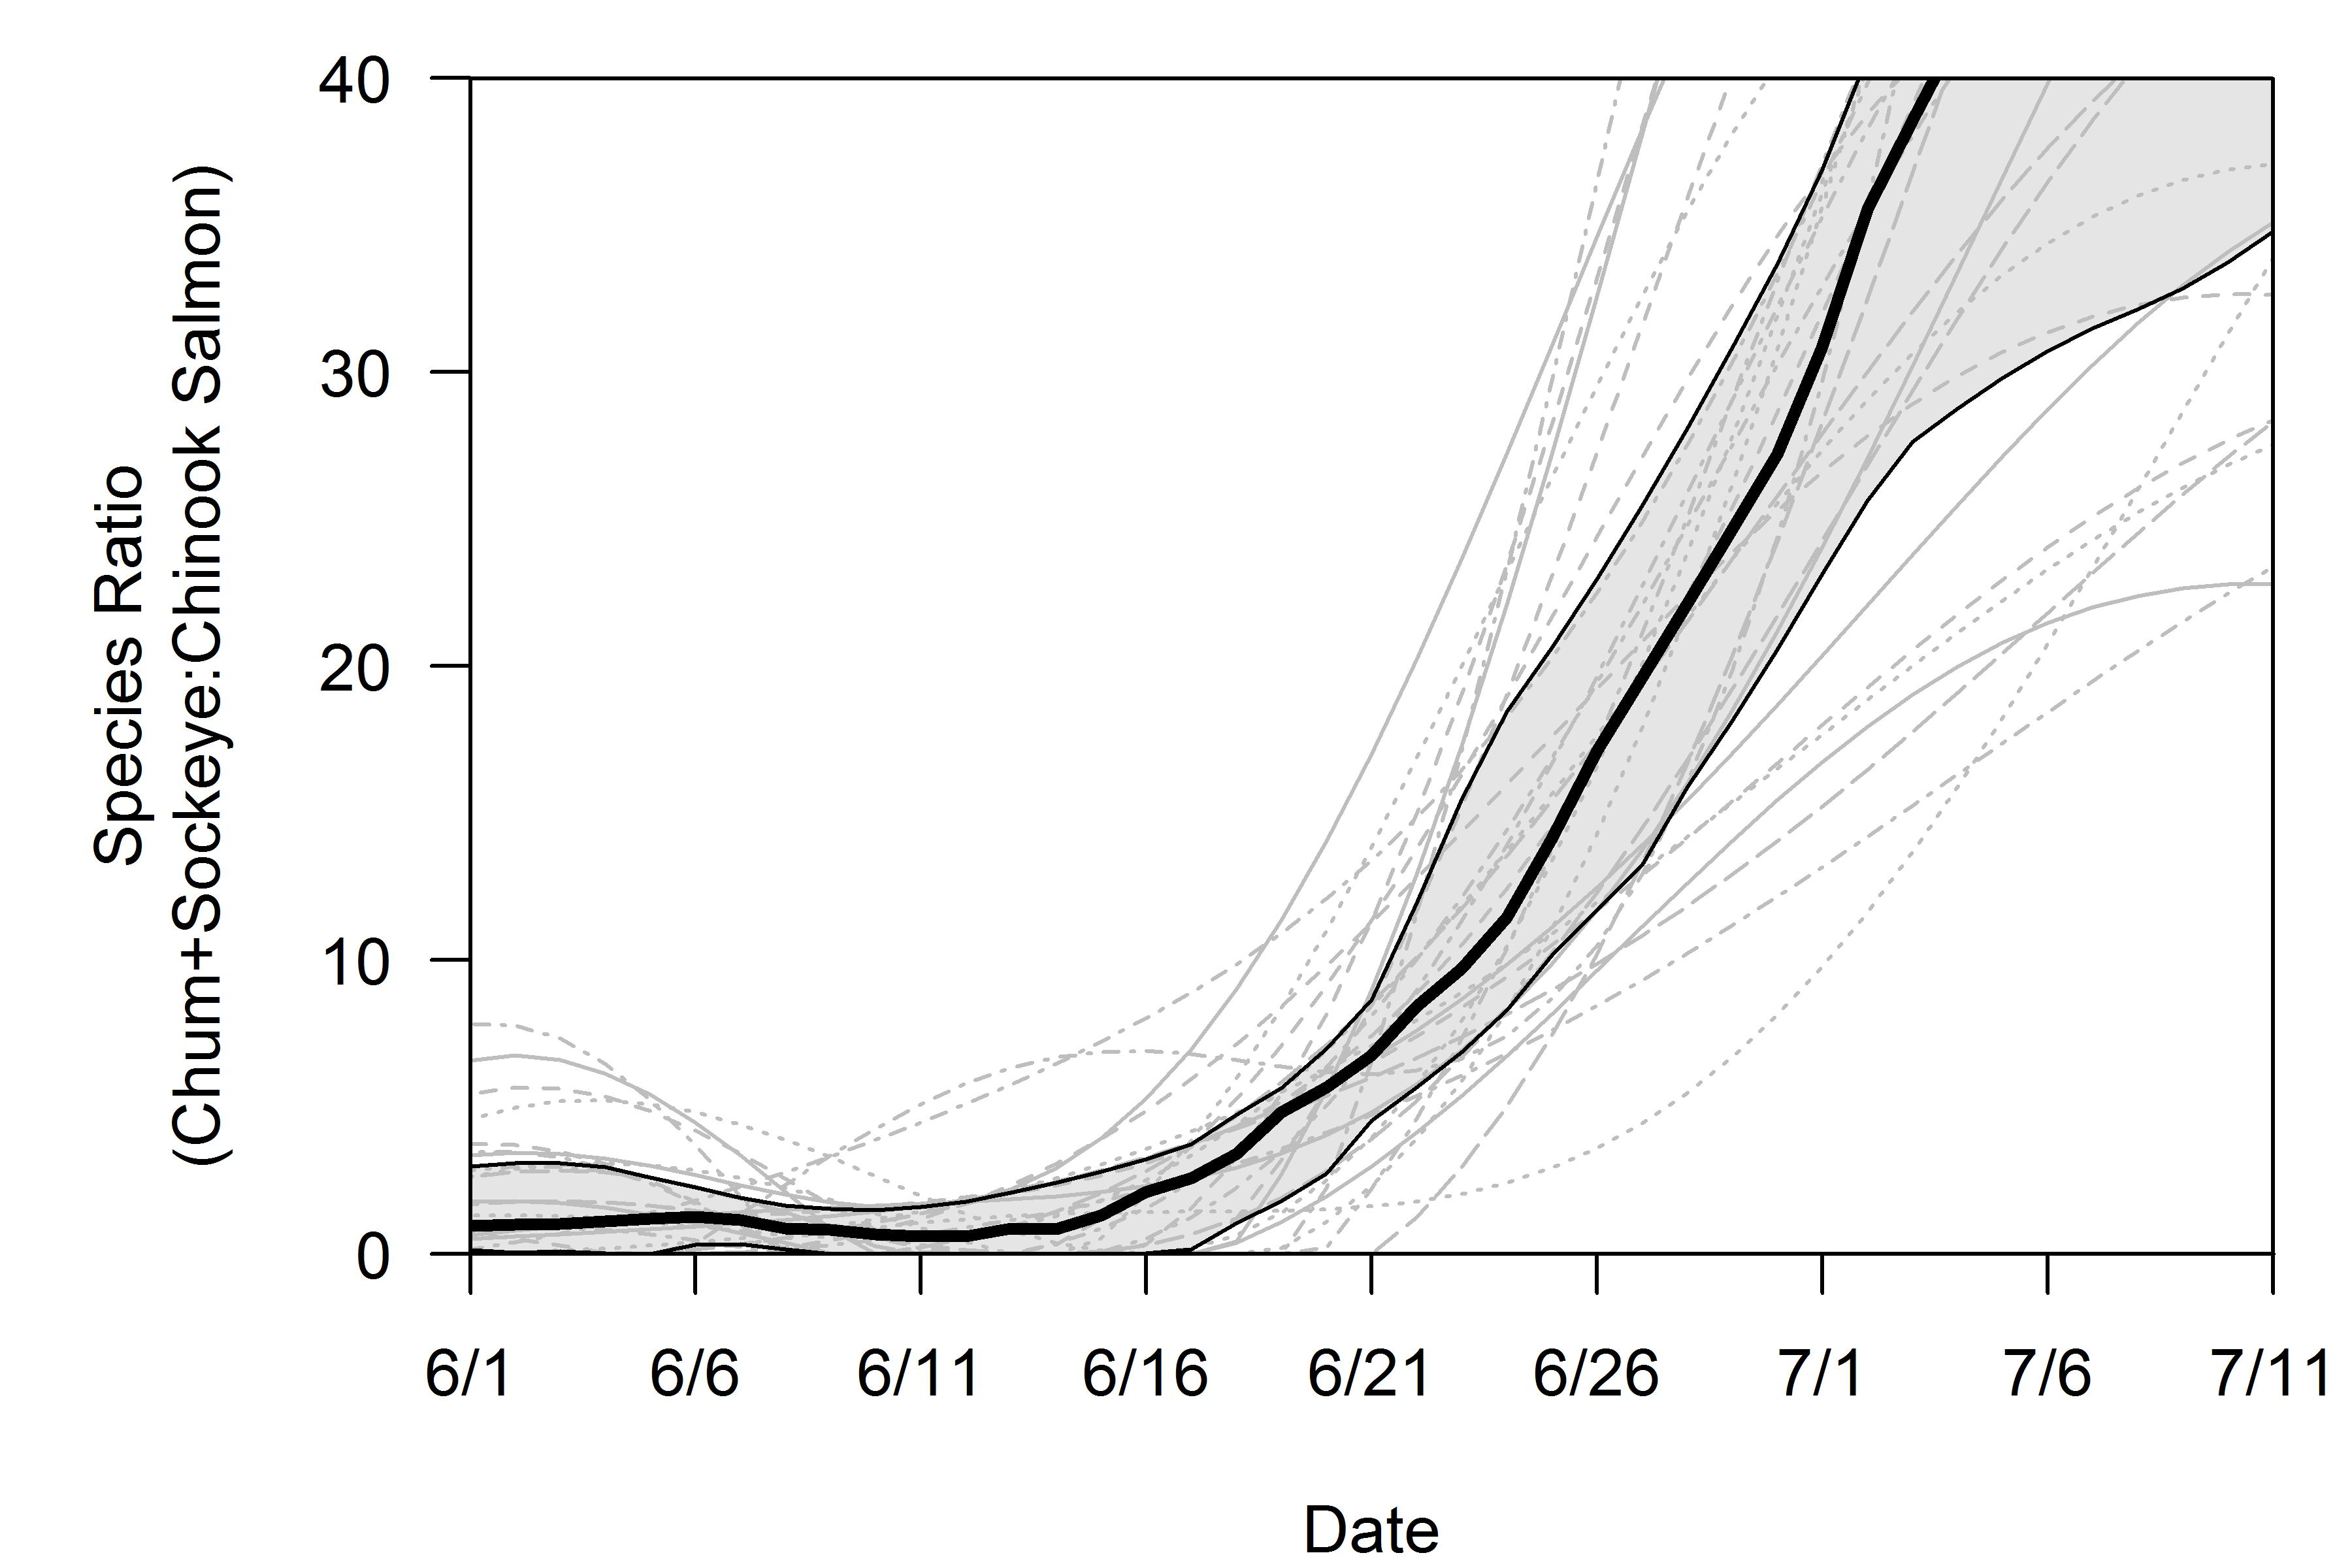
\includegraphics{img/Ch3/ratios-plot.jpg}
  \caption{Smoothed species ratios of chum+sockeye:Chinook salmon as detected by the Bethel Test Fishery. Individual grey lines represent separate years from 1984 -- 2017, the grey region represents the central 50\% of all smoothed ratios on each day and the thick black line represents the daily median. Only this time period is shown because at ratios larger than 20, the differences in the influence of chum/sockeye salmon on Chinook salmon harvest by the subsistence fishery are negligable.}
  \label{fig:ratios-plot}
\end{figure}

\clearpage

\doublespacing

\chapter{Validation of the Operating Model in Chapter
\ref{ch3}}\label{appendix-b}

\noindent
For any simulation model used in the context of management strategy
evaluation, the reliability of inferences drawn will be conditional on
the ability of the model components to capture the important behavioral
properties of the real system. Here, a brief validation is provided that
the fishery component of the operating model did in fact provide a
reasonable model of the real system when the fishery was unrestricted.

First, it is important that the model be able to replicate the
relationship between total Chinook salmon run size and total subsistence
salmon harvest. Capturing this pattern was important to ensure that the
fishery would not inadvertently harvest an unrealistically large or
small amount of fish in different run sizes than would typically occur,
which would confound the inference regarding strategy performance. As
shown in Figure \ref{fig:HvN}, this historical relationship has been
quite noisy for the observed historical time series, though an
increasing pattern has emerged: in general, more fish have been
harvested in years with large runs than years with small runs. It was
found that by tuning the catchability (\(q\)) and effort response
coefficients, this pattern could be reproduced quite well. Additionally,
the scale and variability of modeled chum/sockeye harvests were also
similar to the historically-observed distribution (Figure
\ref{fig:chsk-harvest}) -- this was not key given chum/sockeye harvests
did not inform any objectives, but the agreement contributes more
evidence that the effort response model was adequately calibrated.

The next behavior of interest was the spatiotemporal distribution of
harvest. Because in-river salmon fisheries are sequential, fish
harvested in one area are invulnerable to harvest (and escapement) in
upriver areas. It also means that communities in downriver communities
may finish fishing earlier in the season because they are the first to
experience favorable fishing conditions (i.e., high in-river abundance
and resulting catch rates; in the Kuskokwim River drying weather also
plays an important role). If the timing of harvest was not captured
adequately, this would be an indication that the effort response
coefficients were improperly tuned and could result in unrealistic
conclusions. The patterns and variability in the day of the year at
which various percentiles of Chinook salmon harvest was attained by
reach compared between observed data and the modeled outcomes are shown
in Figure \ref{fig:temporal-harvest}. It seems that the patterns and
variability in harvest timing were reasonably well-captured,
particularly for downriver reaches. Reaches 14, 15, 16 and 22 seemed to
have had the largest deviations between observed and modeled patterns,
but given communities in these reaches harvest a negligible amount of
Chinook salmon in comparison to the downriver villages (Figure
\ref{fig:spatial-harvest}), this finding is not concerning.

The final important characteristic was the spatial distribution of
end-of-season harvest. Accurately representing this component of the
system would further indicate model adequacy. Figure
\ref{fig:spatial-harvest}) shows a comparison of the proportion of total
drainage-wide Chinook salmon subsistence harvest attributable to
communities in each reach between observed and modeled outcomes. While
the overall pattern was fully captured, there were moderate deviations
between the model and observations in reaches 2, 3, and 4.

\clearpage

\begin{figure}
  \centering
  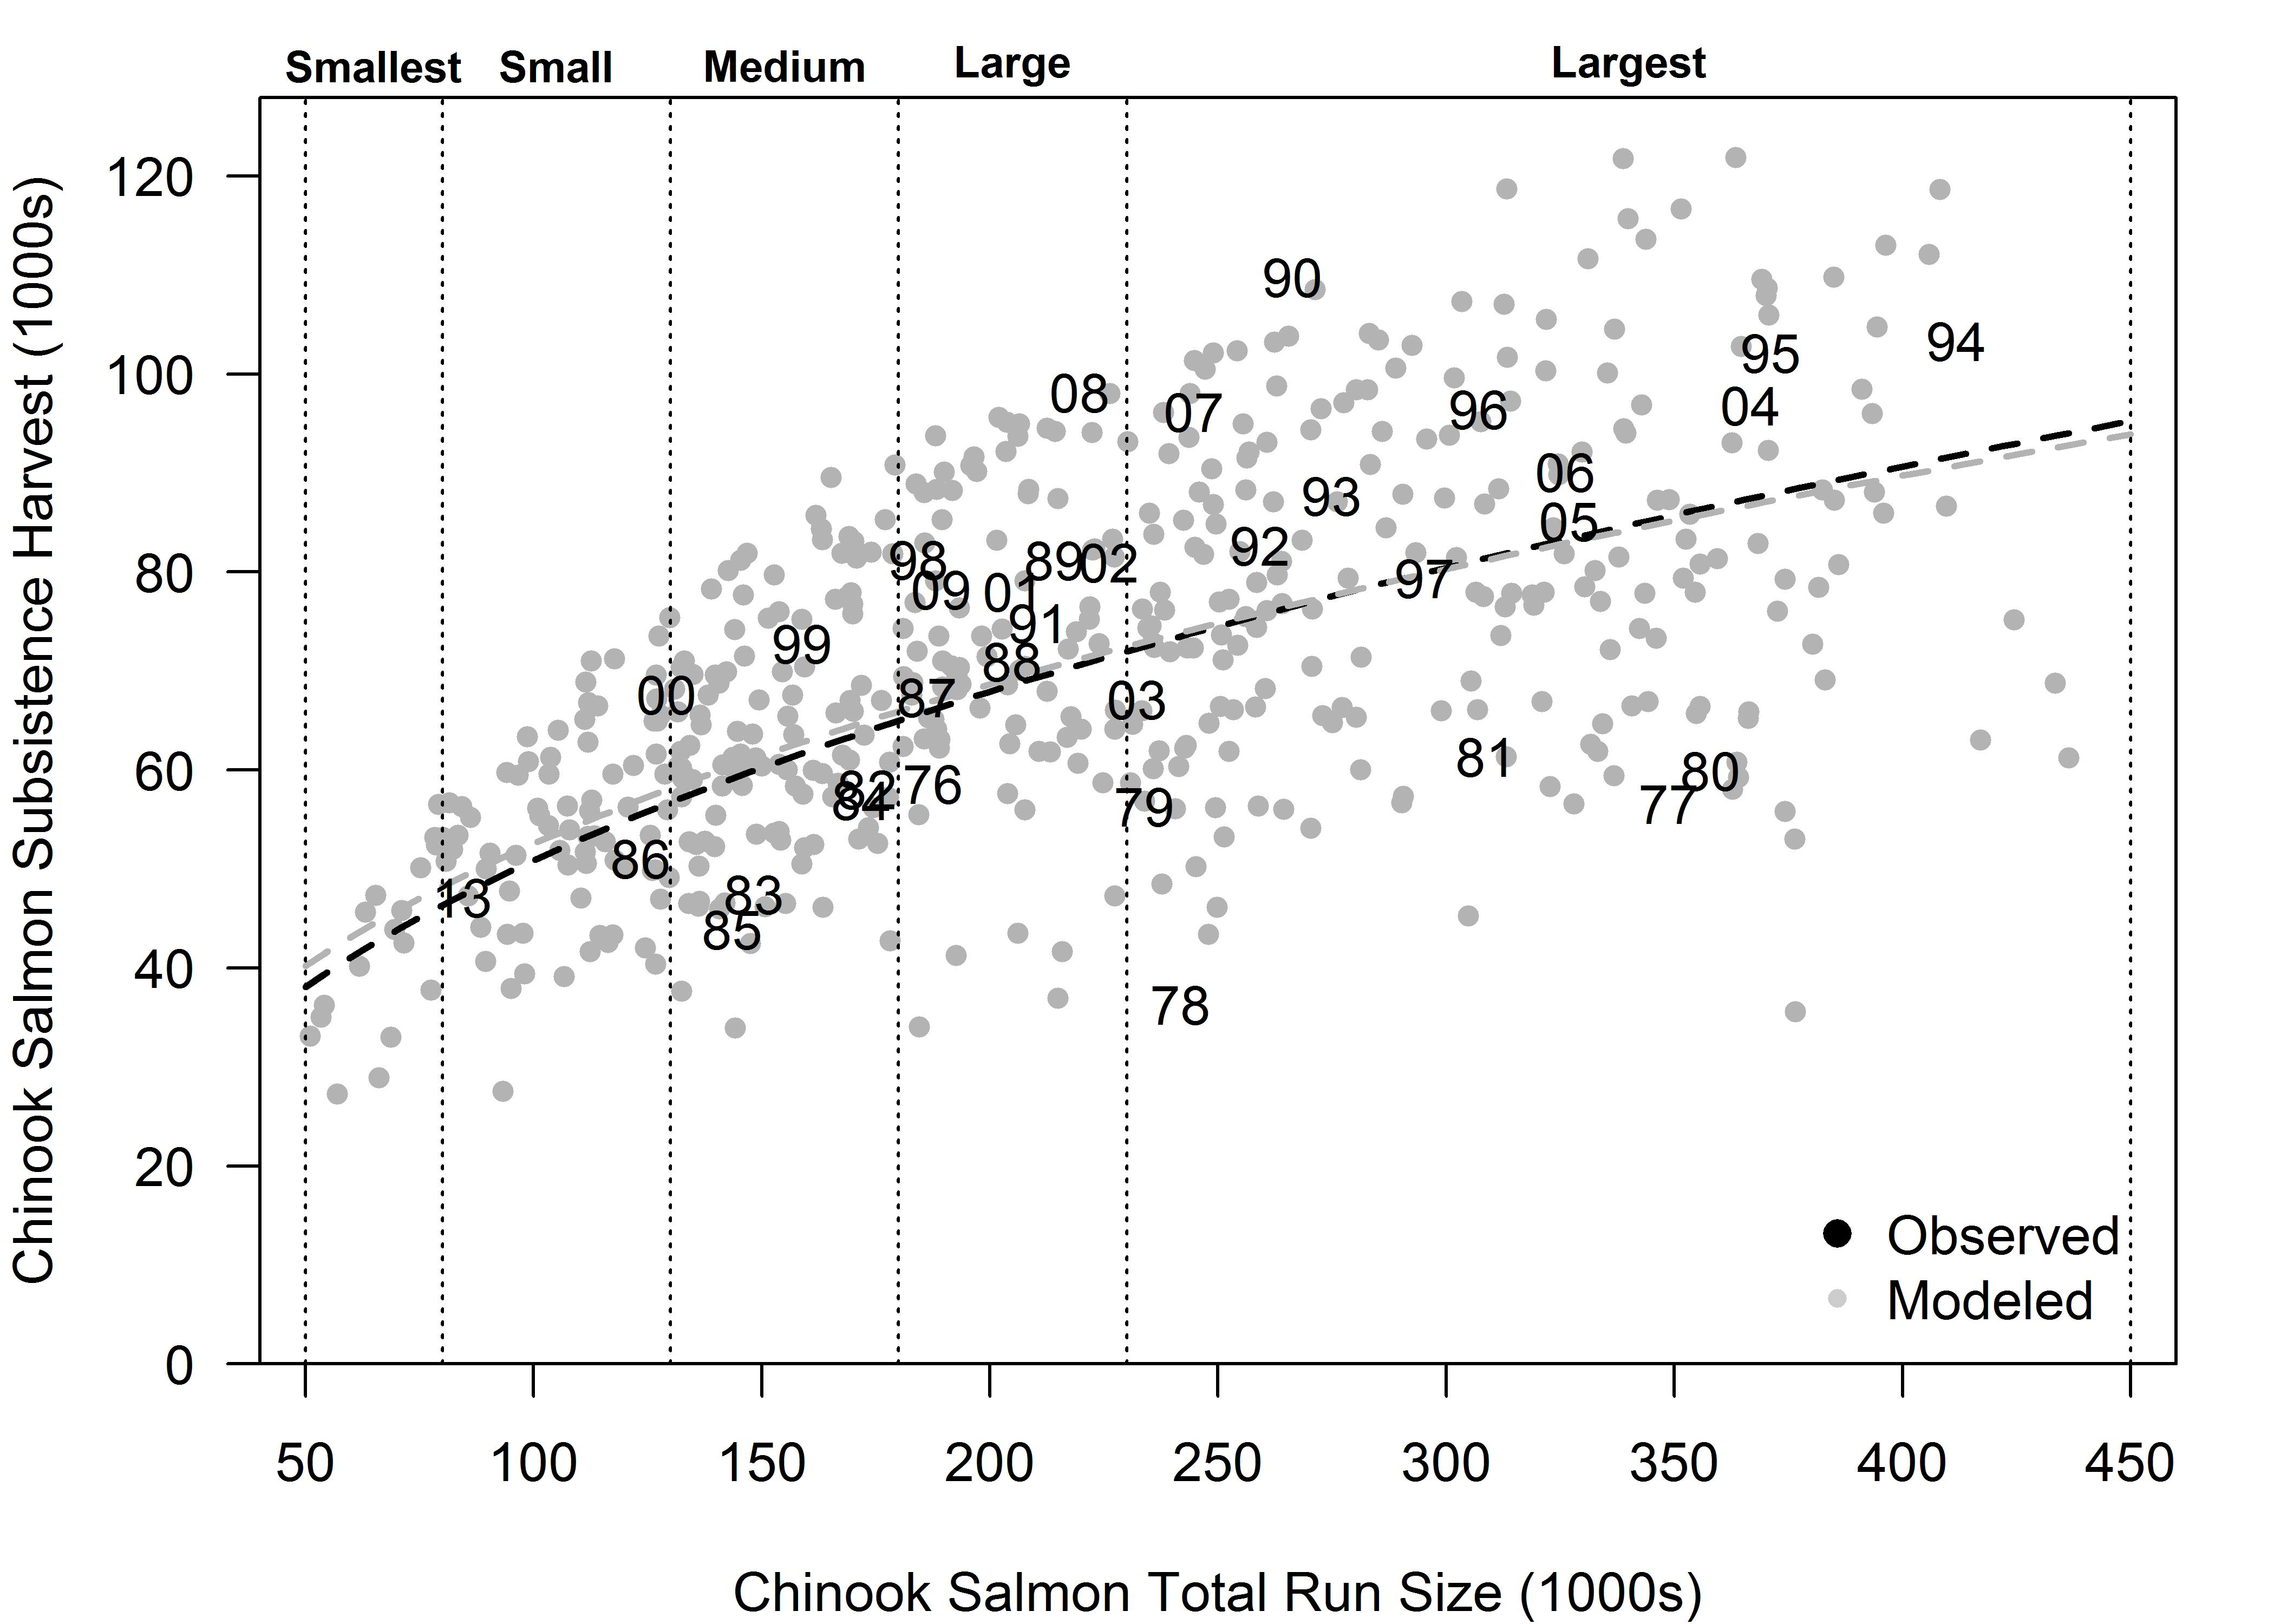
\includegraphics{img/Ch3/Figure B1.jpg}
  \caption{Observed and modeled Chinook salmon subsistence harvest as a function of total Chinook salmon run size. Individual black numbers are historical realizations in years with no harvest restrictions on the subsistence salmon fishery. Individual grey dots are modeled outcomes, each representing a hypothetical salmon run with different random subpopulation compositions, run timing, and species ratios. Fitted models display close agreement between the average simulated and observed harvest outcomes across the range of run sizes. Vertical dotted lines show the important run size strata used in this analysis.}
  \label{fig:HvN}
\end{figure}

\begin{figure}
  \centering
  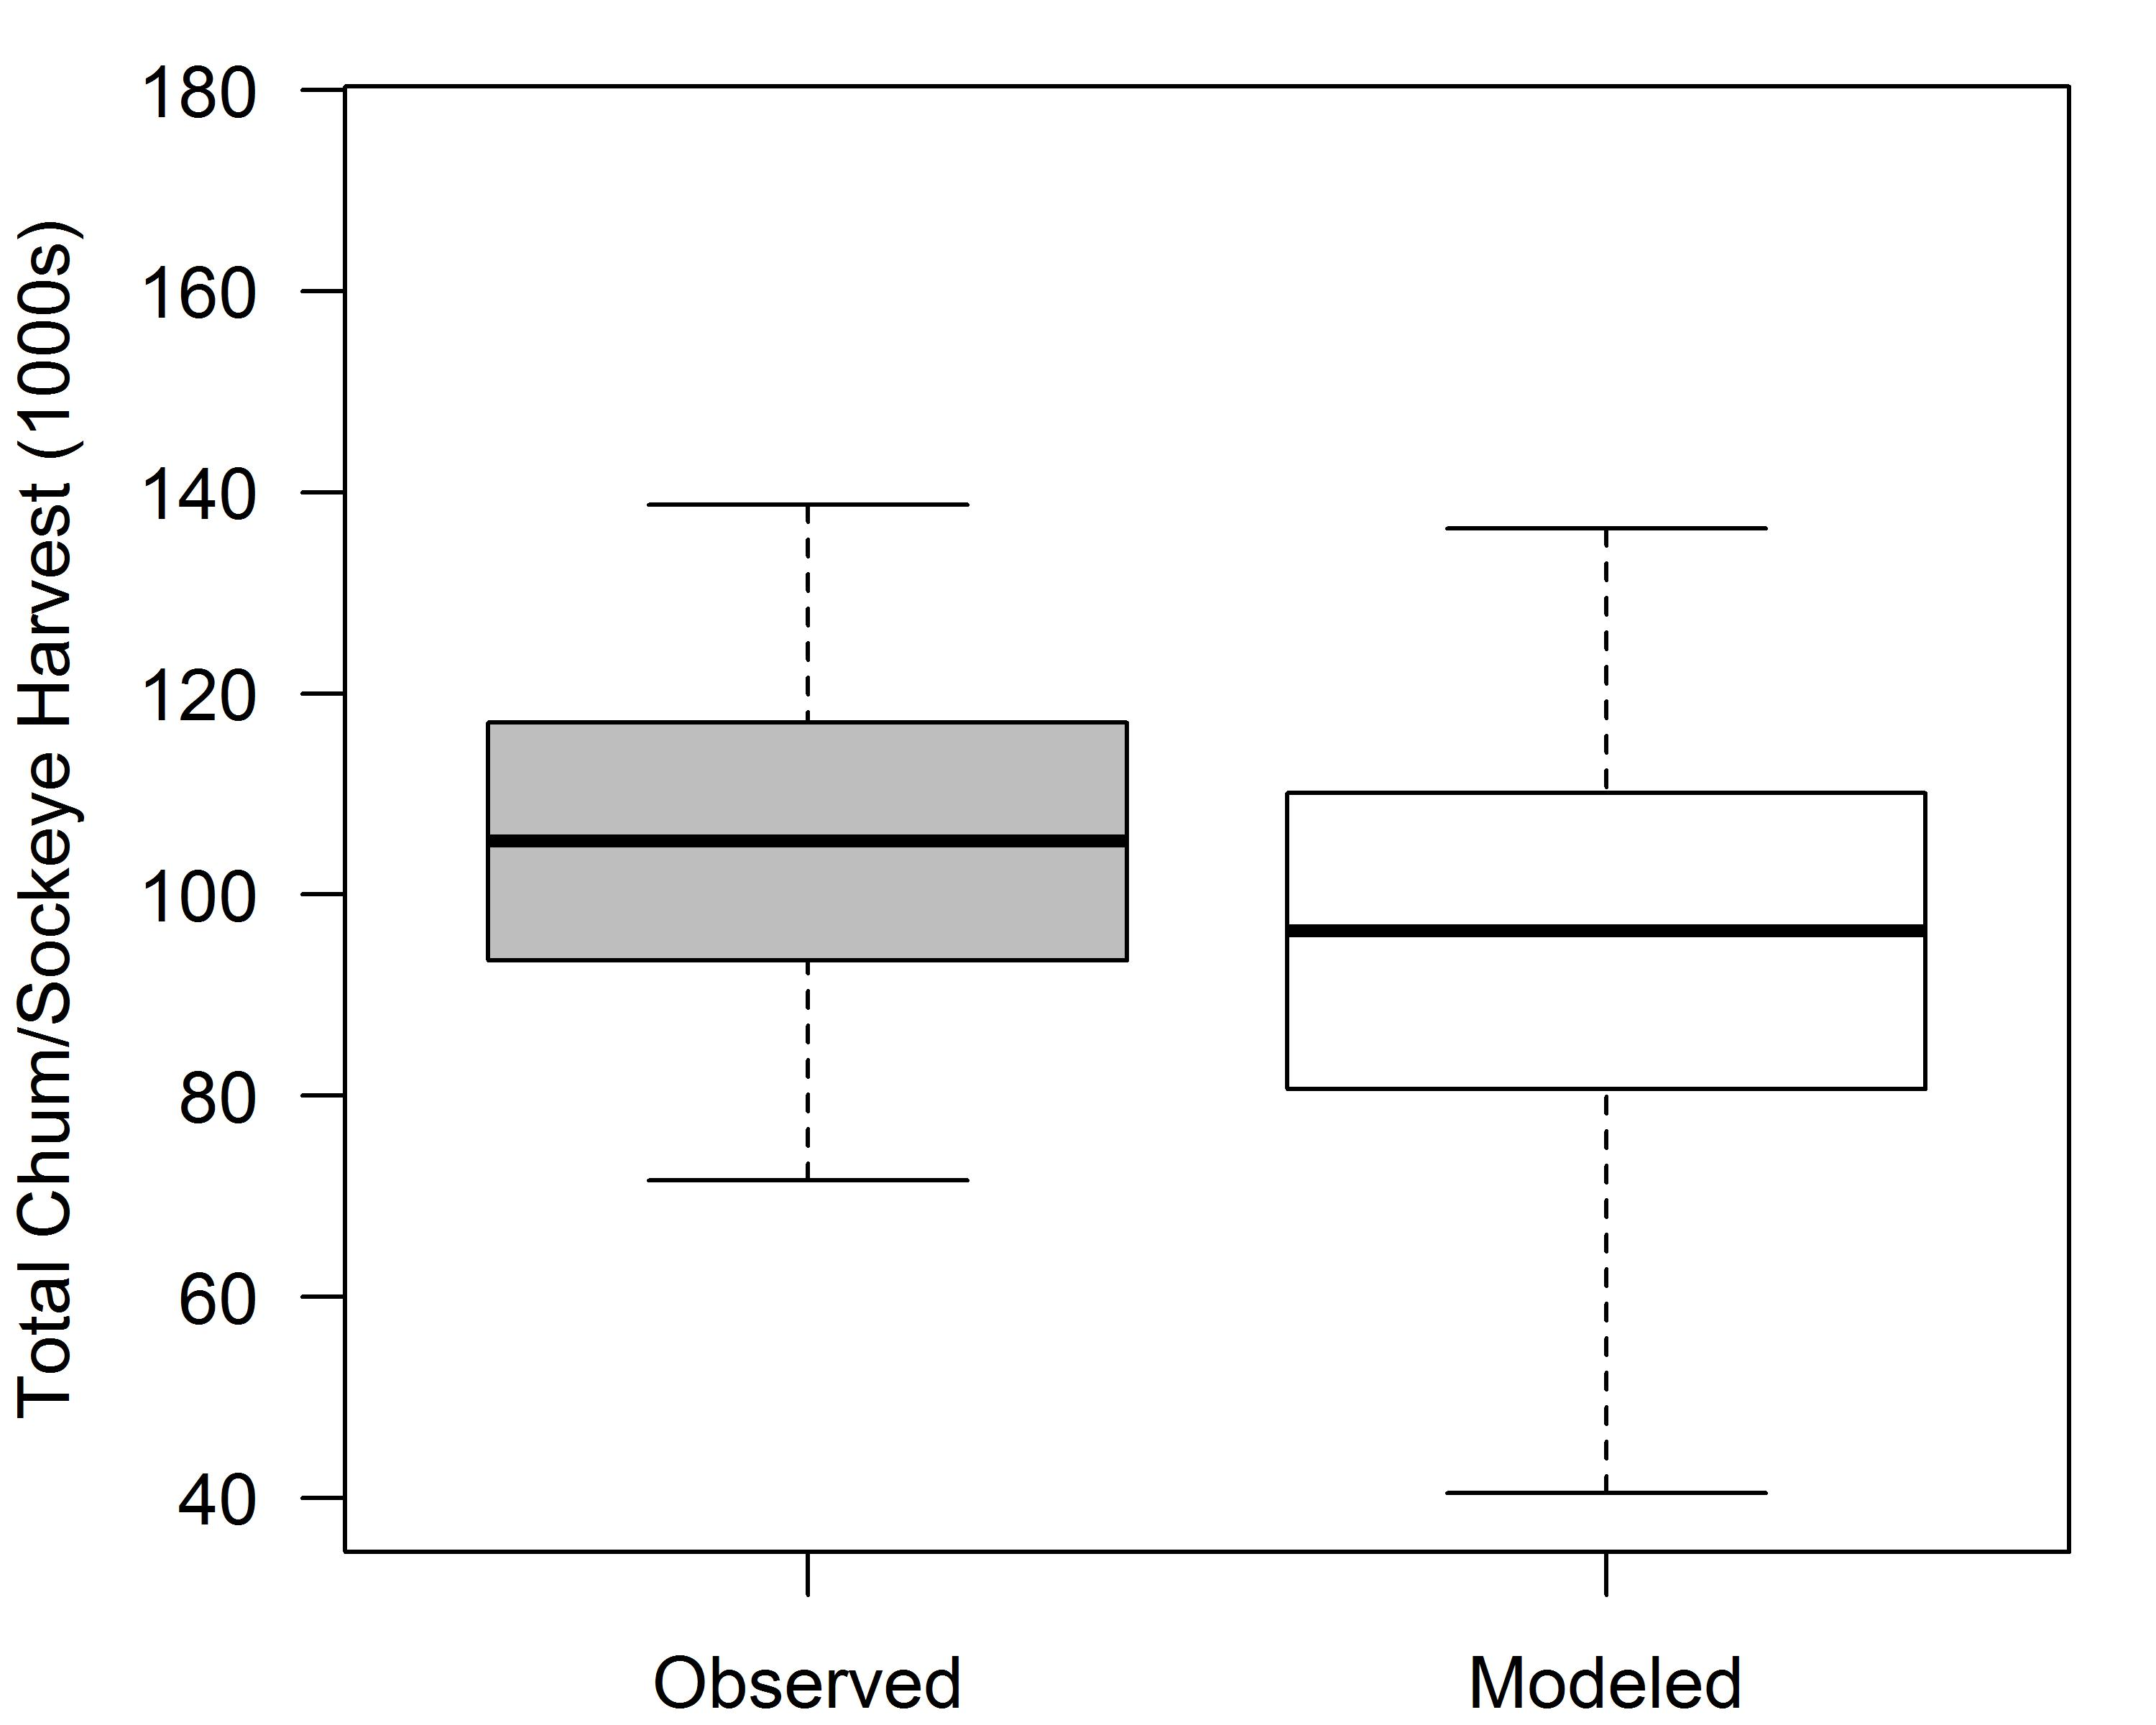
\includegraphics{img/Ch3/Figure B2.jpg}
  \caption{Comparison of the inter-annual distribution of observed and modeled chum/sockeye salmon harvests by villages located in the Kuskokwim River.}
  \label{fig:chsk-harvest}
\end{figure}

\clearpage

\begin{figure}
  \centering
  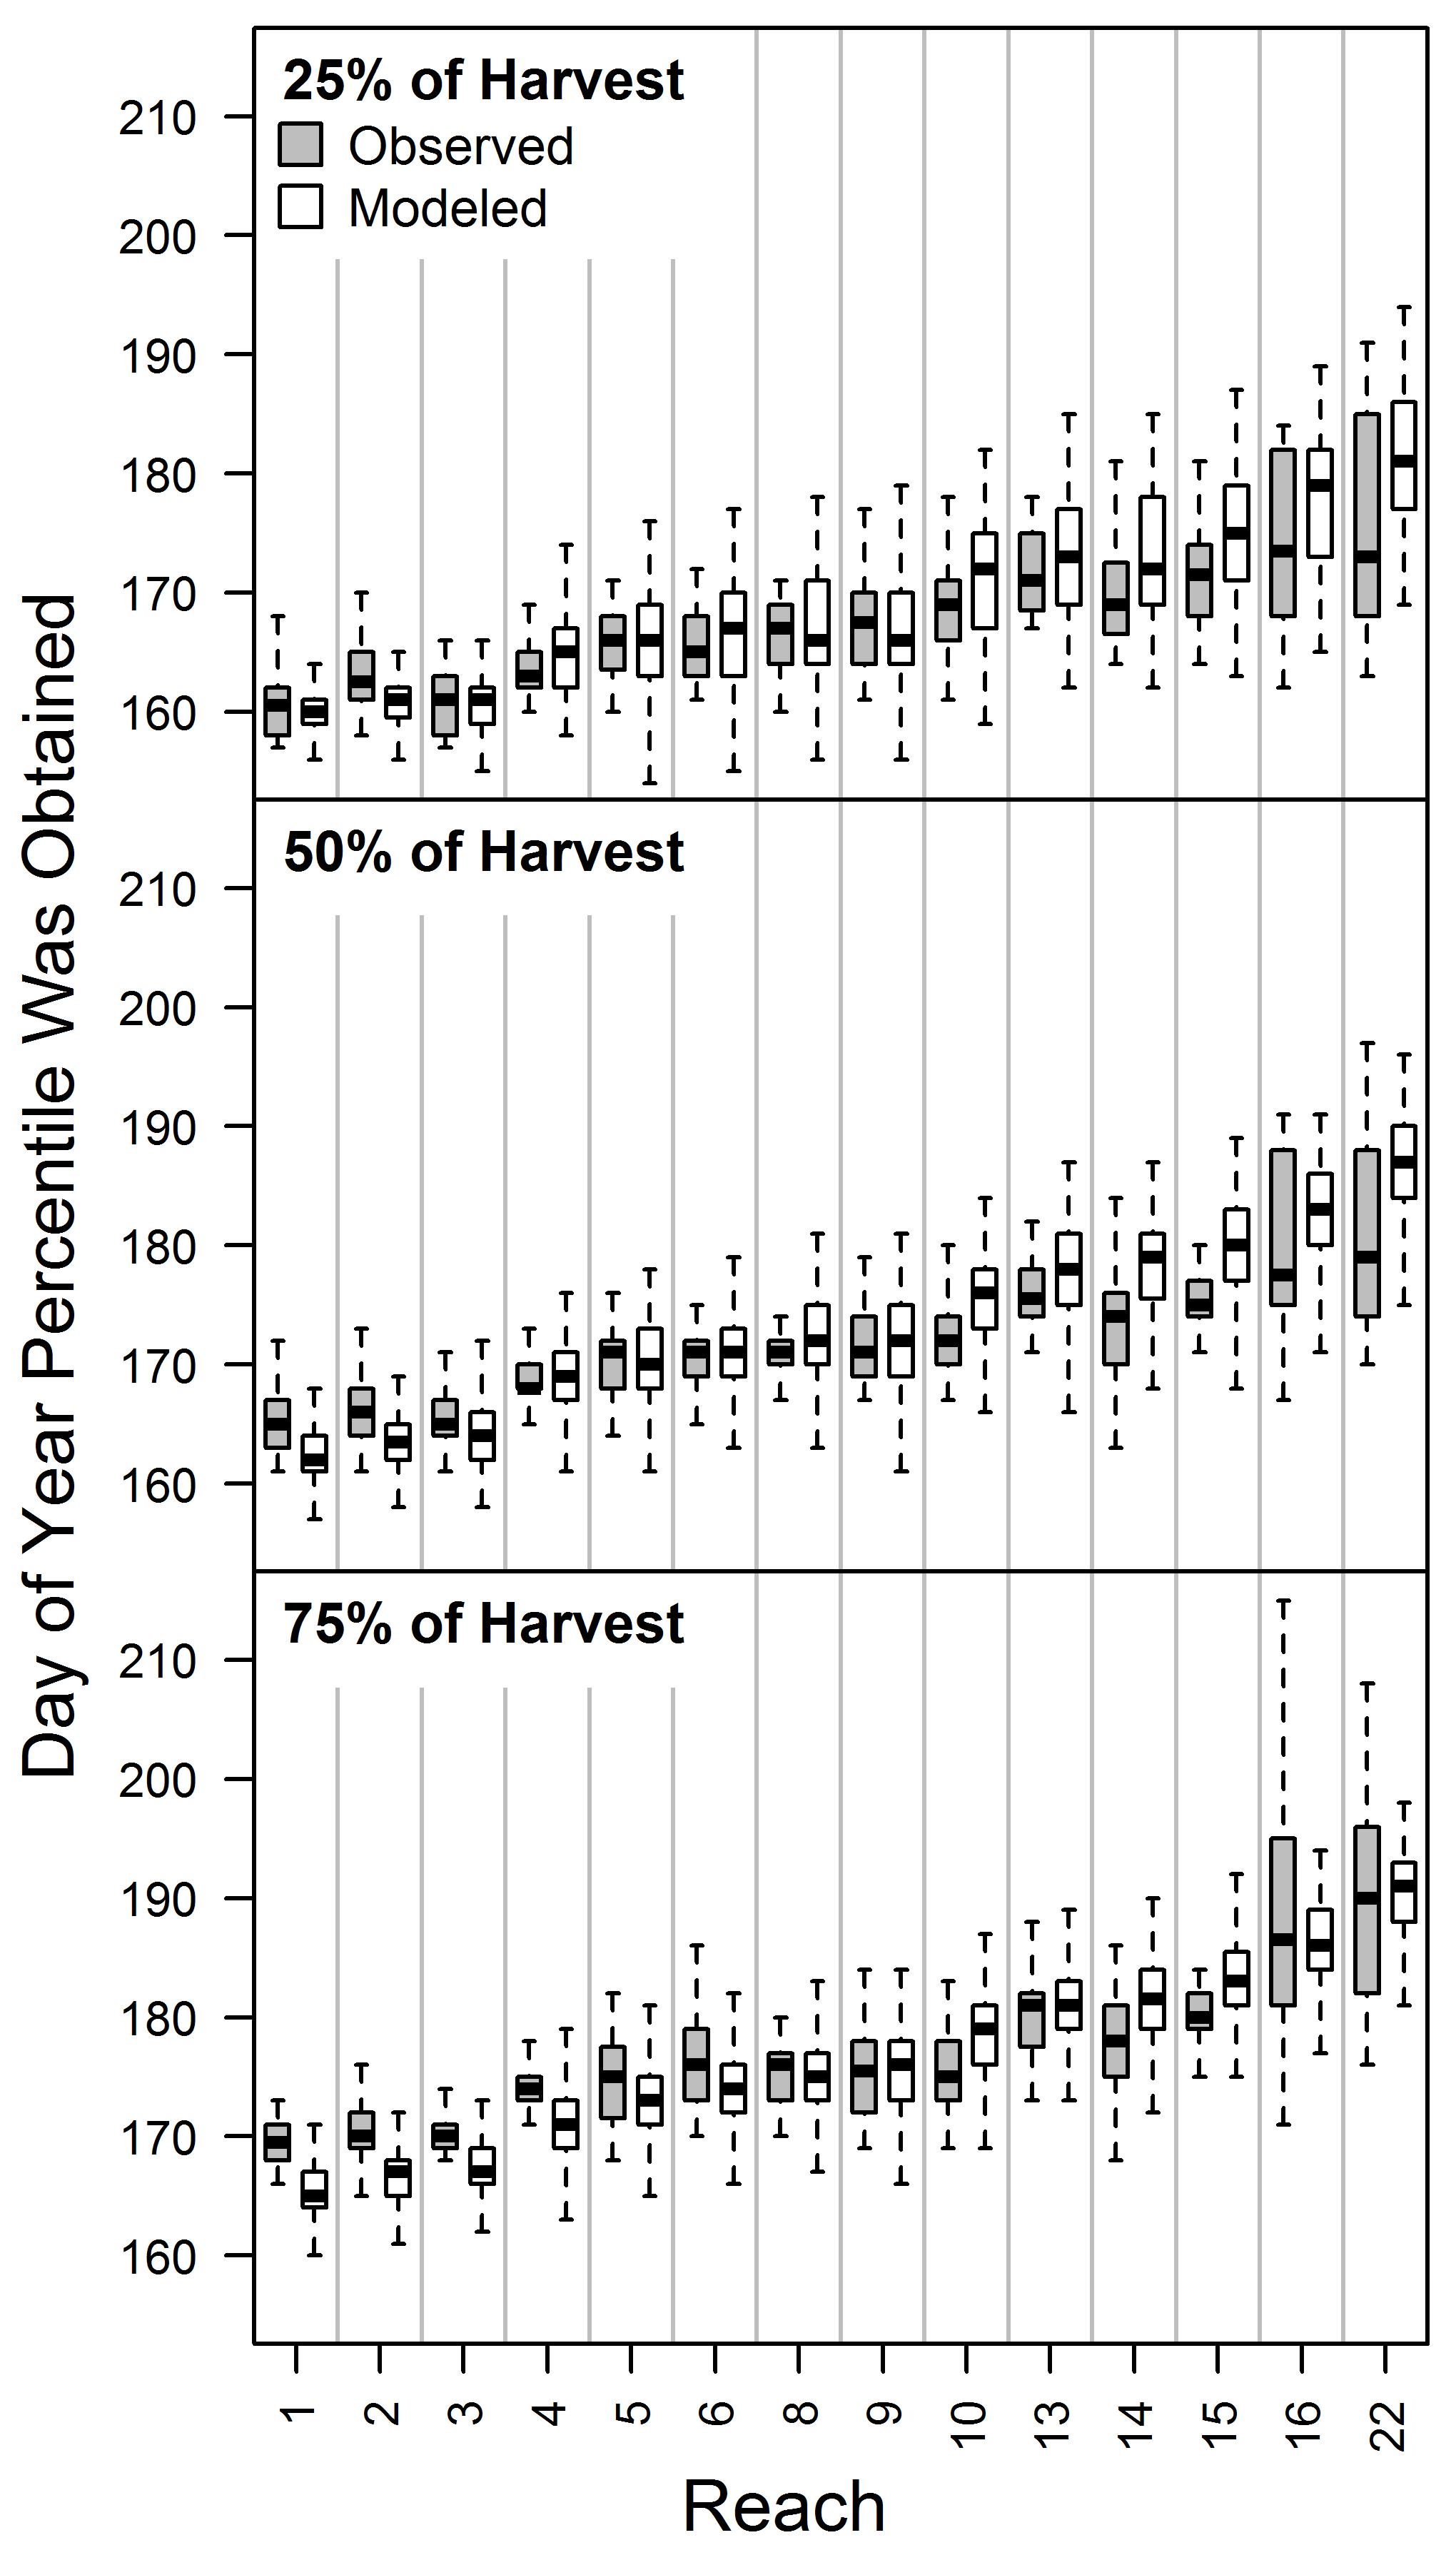
\includegraphics{img/Ch3/Figure B3.jpg}
  \caption{Comparison of the day of the year at which various percentiles of Chinook salmon harvest was attained by reach between observed and modeled outcomes. Variability in the observed boxplots is due to inter-annual variability in run size and timing and represents between-simulation variability for the modeled outcomes. Reach numbers are ordered from downriver to upriver. Note that not all reaches contain communities that harvest salmon.}
  \label{fig:temporal-harvest}
\end{figure}

\clearpage

\begin{figure}
  \centering
  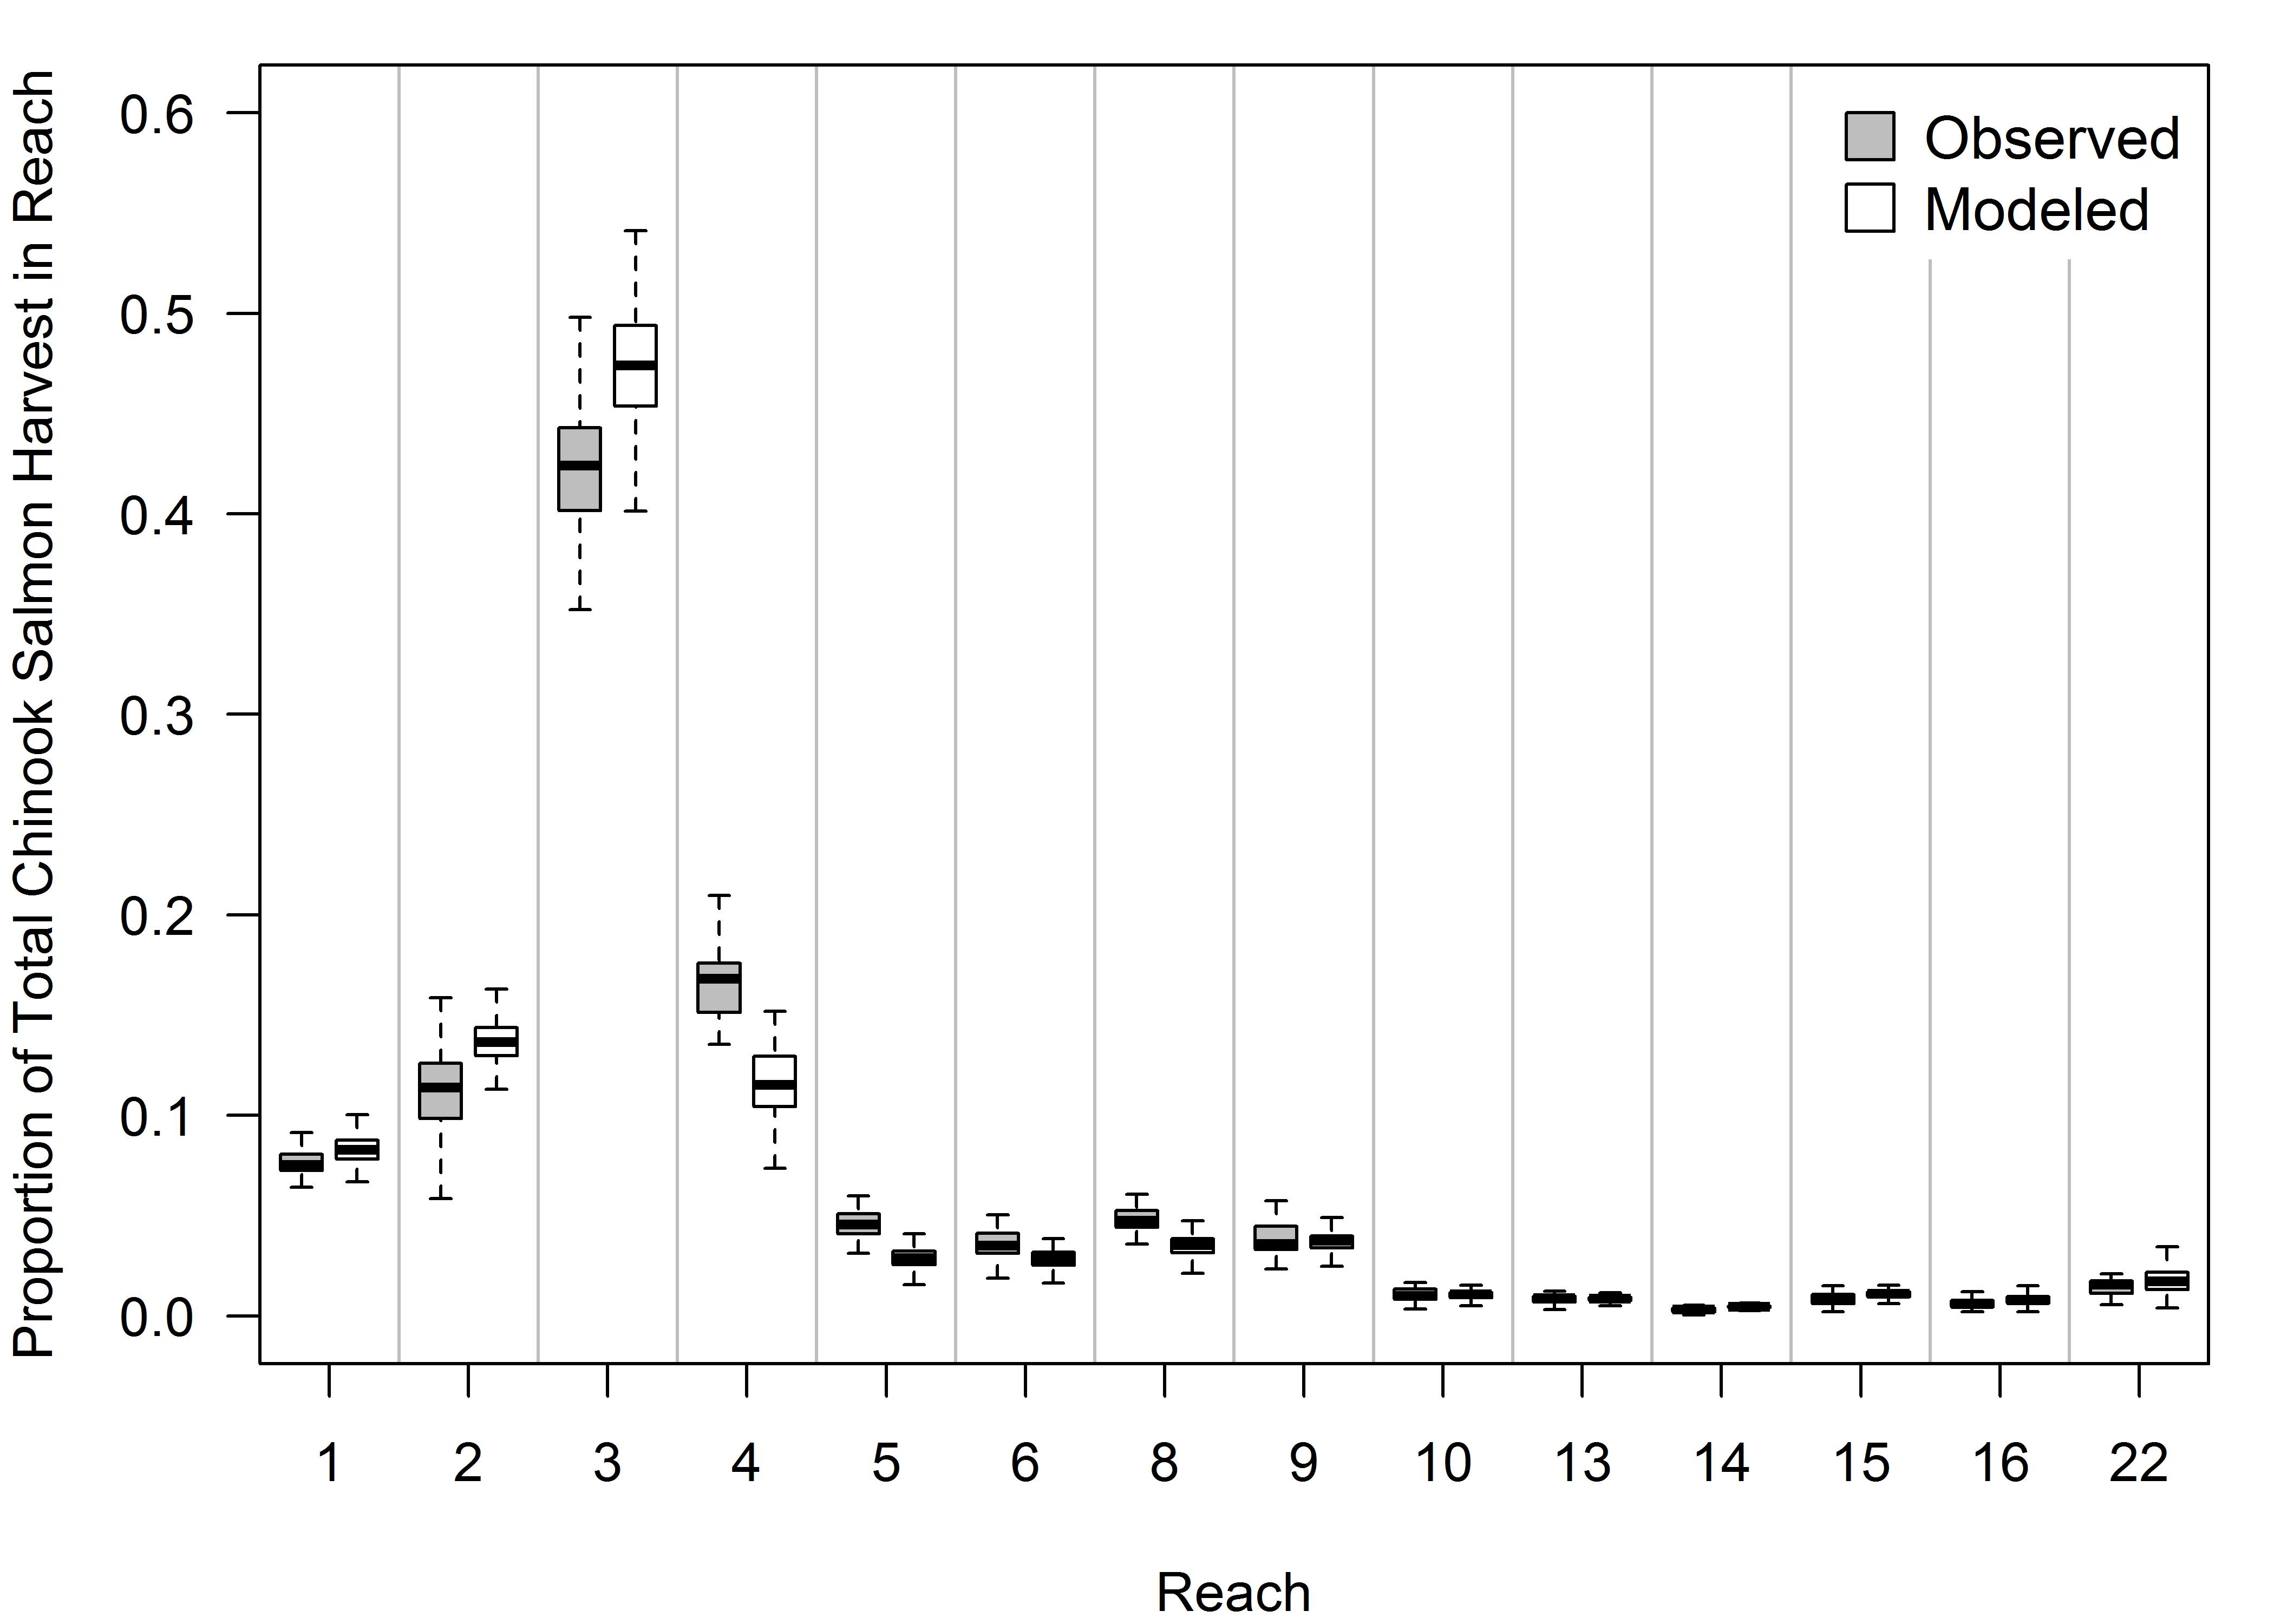
\includegraphics{img/Ch3/Figure B4.jpg}
  \caption{Comparison of the proportion of total drainage-wide Chinook salmon subsistence harvest attributable to communities in each reach between observed and modeled outcomes. Variability in the observed boxplots is due to inter-annual variability, and represents between-simulation variability for the modeled outcomes. Reach numbers are ordered from downriver to upriver. Note that not all reaches contain communities that harvest salmon.}
  \label{fig:spatial-harvest}
\end{figure}

\chapter{Preparation of Data for Fitting Spawner-Recruit Models to
Substocks of Kuskokwim River Chinook Salmon in Chapter
\ref{ch4}}\label{appendix-c}

\section{Overview of data needs}\label{overview-of-data-needs}

\noindent
All data for this analysis are available to the public, and came
primarily from the Arctic-Yukon-Kuskokwim Database Management System
(AYKDBMS)\footnote{\url{http://www.adfg.alaska.gov/CommFishR3/WebSite/AYKDBMSWebsite/Default.aspx}}
maintained by the Alaska Department of Fish and Game (ADF\&G). Cases in
which other data sources were necessary are highlighted in the
description below, e.g., the telemetry data needed to perform the
expansion of aerial survey counts described in Section
\ref{air-expansion} below.

\noindent
This analysis required three primary data sources:

\begin{enumerate}
\def\labelenumi{(\arabic{enumi})}
\item
  Estimates of annual escapement to each of the substocks included.
\item
  Estimates of annual harvest. Linear regression models (Section
  \ref{reg-methods}) required harvest apportioned to each substock, the
  state-space models (Section \ref{ssm-model}) required only total
  aggregate harvest summed across all substocks included.
\item
  Estimates of annual age composition (i.e., the fraction of the run
  each year made up of each age) for all substocks that have had it
  collected.
\end{enumerate}

\noindent
Any of these data sources could have missing years.

\section{Substock escapement}\label{air-expansion}

\noindent
Escapement count data for this analysis were informed predominately by
the ADF\&G Kuskokwim River salmon escapement monitoring program, the
details of which have been most-recently documented in
\citet{head-smith-2018}. The data set available spanned 20 different
escapement monitoring projects (six weirs and 14 aerial surveys) and 42
calendar years from 1976 -- 2017, though monitoring projects differed in
the date they were initialized (Figure \ref{fig:obs-freq}). For
substocks monitored \emph{via} weir, observed escapement for substock
\(j\) in year \(t\) (\(S_{obs,t,j}\)) was taken to be the total
estimated weir passage each year. Substocks monitored \emph{via} aerial
survey needed special care, however. Surveys have been flown only once
per year on a relatively small fraction of each tributary system (Figure
\ref{fig:ch4-map}), resulting in these data being indices of escapement
rather than estimates of total escapement to the subdrainage. This
analysis required estimates of total escapement to each substock
however, because this would allow calculation of biological reference
points that are expressed in terms of the scale of the population (e.g.,
the spawner abundance that is expected to produce maximum recruitment;
\(S_{\text{MAX},j}\)), rather than as a rate (i.e.,
\(U_{\text{MSY},j}\)). Note that if only estimates of
\(U_{\text{MSY},j}\) were desired, no accounting for the partial counts
would be necessary.

The approach I developed to estimate total escapement from single-pass
aerial surveys involved two main steps:

\begin{enumerate}
\def\labelenumi{(\arabic{enumi})}
\item
  Mapping the distribution of detected telemetry-tagged Chinook salmon
  against distribution of the aerial survey counts. This comparison
  allowed for a spatial expansion to estimate how many salmon would have
  been counted had the entire tributary been flown. Radio telemetry
  studies targeting Chinook salmon in the Kuskokwim River have been
  conducted intermittently since the early 2000s, and data were used
  from the years 2003 -- 2007 and 2015 -- 2016. These studies tagged
  fish migrating through the middle or lower river and (among other
  things) located them at the end of the season using aerial telemetry
  \citep{stuby-2007, smith-liller-2017a, smith-liller-2017b}.
\item
  Obtaining and applying a temporal correction factor for the problem of
  counting a dynamic pool at one point in its trajectory. This
  correction factor was based on the relationship between paired weir
  and aerial counts on \(n=3\) of the systems in the analysis.
\end{enumerate}

\subsection{Spatial expansion}\label{spat-expansion}

\noindent
The core of the the spatial expansion estimator was the assumption:

\begin{equation}
  \frac{A_{f,t,i}}{T_{f,t,i}} = \frac{A_{u,t,i}}{T_{u,t,i}},
  \label{eq:air-expand1}
\end{equation}

\noindent
where the quantities \(A\) and \(T\) represent fish and tags,
respectively, in flown (\(A_f\) and \(T_f\)) and unflown (\(A_u\) and
\(T_u\)) reaches in year \(t\) and for aerial survey monitoring project
\(i\). This assumption states that the ratio of actual spawners per one
tagged spawner is the same between flown and unflown river sections at
the time of the aerial index count and the aerial telemetry flights.
Equation \eqref{eq:air-expand1} and can be rearranged as:

\begin{equation}
  A_{u,t,i} = A_{f,t,i} \frac{T_{u,t,j}}{T_{f,t,i}}.
  \label{eq:air-expand2}
\end{equation}

\noindent
If \(T_{u,t,i}\) is further assumed to be a binomial random variable
with time-constant success parameter \(p_i\), then:

\begin{equation}
  T_{u,t,i} \sim \text{Binomial}(p_i,T_{u,t,i} + T_{f,t,i}).
  \label{eq:air-expand-binomial}
\end{equation}

\noindent
Here, \(p_i\) represents the probability that a tagged fish in the
spawning tributary monitored by project \(i\) was outside of the survey
flight reach at the time of the aerial telemetry flight. When
\eqref{eq:air-expand-binomial} is rearranged to put \(p_i\) on the odds
scale, then:

\begin{equation}
  \psi_i=\frac{p_i}{1-p_i}.
  \label{eq:air-expand-odds}
\end{equation}

\noindent
The odds value \(\psi_i\) can be substituted for the division term in
\eqref{eq:air-expand2} which gives:

\begin{equation}
  A_{u,t,i} = A_{f,t,i} \psi_i.
  \label{eq:air-expand3}
\end{equation}

\noindent
To obtain the total number of fish that would have been counted had the
entire subdrainage been flown (\(\hat{A}_{t,i}\)), the components can be
summed:

\begin{equation}
  \hat{A}_{t,i} = A_{f,t,i} + A_{u,t,i}.
  \label{eq:air-expand4}
\end{equation}

\noindent
Substitution of \eqref{eq:air-expand3} into \eqref{eq:air-expand4} and
factoring gives the estimator:

\begin{equation}
  \hat{A}_{t,i}=A_{f,t,i}(1 + \psi_i).
  \label{eq:air-expand-final}
\end{equation}

\noindent
The spatial expansion model was integrated with the temporal expansion
model described below into a single model fitted in the Bayesian
framework fitted using JAGS \citep{plummer-2017}. This allowed for
seamless propagation of uncertainty (in \(\psi_i\)) from the expansion
above to the next step.

\subsection{Temporal Expansion}\label{temp-expansion}

\noindent
A temporal expansion model was necessary to convert from the one-pass
index scale to the substock total annual escapement scale. The temporal
expansion I developed operated by first regressing \(n = 16\)
observations of paired weir count (\(W_i\)) and spatially-expanded
aerial counts (\(\hat{A}_{i}\); given by \eqref{eq:air-expand-final}) on
the same tributary systems (\(n = 3\)) in the same years:

\begin{equation}
  \begin{split}
    W_i = \beta_0 + \beta_1 \hat{A}_i + \varepsilon_i, \\
    \varepsilon_i \stackrel{\text{iid}}{\sim} N(0, \sigma_W) \\
  \end{split}
\label{eq:temp-expand1}
\end{equation}

The estimated coefficients \(\hat{\beta}_0\) and \(\hat{\beta}_1\)
(Table \ref{tab:temp-expand-table}) were then applied to tributary
systems with an aerial count but not a weir count:

\begin{equation}
  S_{obs,t,j}=\hat{\beta}_0 + \hat{\beta}_1 \hat{A}_{t,j}
\label{eq:temp-expand2}
\end{equation}

\noindent
The fitted relationship is shown in Figure \ref{fig:obs-correct}. For
substocks that had both weirs and aerial surveys, the weir count was
used as \(S_{obs,t,j}\) as opposed to using the expansion in
\eqref{eq:temp-expand2} and the coefficient of variation (CV) representing
observation uncertainty for the state-space models was set at 5\%, which
assumed annual escapement counts made at weirs are made with little
measurement error. For substocks monitored solely \emph{via} aerial
survey, the posterior mean value of \(S_{obs,t,j}\) was used as the
escapement count that year, and the posterior CV was calculated for use
as the observation uncertainty passed to the state-space models.

\section{Aggregate harvest}\label{harv-expansion}

\noindent
Harvest estimates for the Kuskokwim River were available at the
drainage-wide scale only, and were obtained each year by subtracting the
drainage-wide estimates of total run and escapement
\citep{liller-etal-2018}. Because the escapement data used here did not
encompass all the substocks within the Kuskokwim River system, it was
necessary to remove some portion of the total harvest that was produced
by stocks not included in this analysis. First, I calculated the
observed exploitation rate of the drainage-wide Kuskokwim River Chinook
salmon stock (\(U_{obs,t}\)) by dividing the total harvest by the total
run each year. I then made the assumption that monitored and unmonitored
substocks have received the same exploitation rates, in which case total
harvest accounted for in this analysis harvest could be obtained as:

\begin{equation}
  H_{obs,t} = \frac{S_{obs,t} U_{obs,t}}{1-U_{obs,t}},
  \label{eq:H-obs}
\end{equation}

\noindent
which can be derived from the definition of the exploitation rate
\(\left(U = \frac{H}{S+H}\right)\). This step was embedded within the
same Bayesian model that encompassed the spatial and temporal aerial
survey expansions such that uncertainty in these steps could be
propagated through the entire analysis. The posterior mean value of
\(H_{obs,t}\) was used as the observed total harvest data, and the
posterior CV was retained for use as the observation error attributed to
this data source.

Note that \(S_{obs,t}\) and \(H_{obs,t}\) do not have \(j\) subscripts
denoting particular substocks: this indicates that they are aggregate
quantities summed across all substock components. In cases where
substock-specific harvest was required (i.e., in reconstructing the
substock-specific brood tables for fitting regression relationships;
Section \ref{lm-btable}), \(H_{obs,t,j}\) was obtained using
\eqref{eq:H-obs} by substituting \(S_{obs,t,j}\) in for \(S_{obs,t}\).

\section{Age composition}\label{age-comp}

\noindent
Age composition data were necessary to reconstruct brood tables for
age-structured salmon populations (see Section \ref{lm-btable}). Age
data used in this analysis came from the ADF\&G standardized age, sex,
and length sampling program operated at the weir projects. All sampled
fish that were not aged successfully were discarded as were samples
corresponding to the rare ages of 3 and 8 such that only fish
successfully aged as between 4 and 7 were included. It is possible that
older or younger fish may have the systematic tendency to return early
or late in the run, and this could introduce biases if age sampling was
not conducted proportionally to fish passage throughout the season. To
adjust for this possibility, a weighted-average scheme was applied to
obtain the age composition estimates for each substock and year with
data. Daily age samples were stratified into two-week strata and
strata-specific proportions-at-age were calculated. These
strata-specific age compositions were then averaged across strata within
a year and stock weighted by the number of Chinook salmon estimated to
have passed the weir in each stratum. The total number of fish
successfully aged for each year and substock was retained for
data-weighting purposes for the state-space models, which (unlike the
regression-based approaches) internally reconstructed the brood tables.

\section{Brood table reconstruction}\label{lm-btable}

\noindent
An important consideration in the use of the regression-based method
(Section \ref{reg-methods}) is in how the \(\text{RPS}_{y,j}\) data are
obtained for salmon stocks that return at more than one age (like
Chinook salmon). Only the states \(S_{y,j}\) are ever directly observed;
\(R_{y,j}\) is observed (for Chinook salmon) over four calendar years as
not all fish mature and make the spawning migration at the same age.
Thus, in order to completely observe one \(\text{RPS}_{y,j}\) outcome,
escapement must be monitored in year \(y\) and escapement, harvest, and
age composition must be monitored in the subsequent years \(y+4\),
\(y+5\), \(y+6\), and \(y+7\). It is evident that missing one year of
sampling (which is common; Figure \ref{fig:obs-freq}) can lead to issues
with this approach. Only completely observed \(\text{RPS}_{y,j}\) data
were used for this analysis, with the exception of missing age
composition data. For substocks with no age composition data (i.e.,
those monitored \emph{via} aerial survey), the average age composition
each year across substocks that have data was used to reconstruct
\(\text{RPS}_{y,j}\), but was provided only for years with escapement
sampling for substock \(j\). Only substocks with \(\ge3\)
completely-observed pairs of \(\text{RPS}_{y,j}\) and \(S_{y,j}\) were
included for model fitting, given each fitted line was dictated by two
parameters.

\section{Results}\label{results-3}

\subsection{Escapement}\label{esc-data-results}

\noindent
The escapement project that received the largest spatial expansion
factor (\(1 + \hat{\psi}_j\)) was the Holitna River, with an expansion
factor of 4.78 (4.04 -- 5.73; 95\% equal-tailed credible limits) as
shown in Table \ref{tab:spat-expand-table}. Given the small length of
surveyed stream relative to the size of the Holitna subdrainage (Figure
\ref{fig:ch4-map}; substock \#7), this large estimate makes intuitive
sense. The aerial survey project that required the smallest spatial
expansion was the Salmon fork of the Aniak River (1.04; 1.01 -- 1.14;
Table \ref{tab:spat-expand-table}); note that this project captures
nearly all of this tributary of the Aniak sytem (western-most fork of
drainage \#4; Figure \ref{fig:ch4-map}). The average spatial expansion
factor across all aerial survey projects was 1.78 (1.67 -- 1.93).

In terms of the temporal expansion, the estimate for the primary
expansion coefficient (\(\hat{\beta}_1\)) was 2.3 (1.76 -- 2.85; Table
\ref{tab:temp-expand-table}). This estimate indicates that
spatially-corrected aerial survey counts needed to be scaled up by a
factor of 2.3 in order to be consistent with the total annual escapement
counts made at weirs in years and subdrainages that had paired counts.
This estimate makes intuitive sense given ADF\&G has structured the
timing of aerial survey flights to coincide with the peak of the
escapement timing arrival curve \citep{head-smith-2018}, which should
occur approximately halfway through the run, indicating the aerial
counts would need to be doubled to account for the second half of the
run. The freely-estimated intercept of the temporal expansion
(\(\hat{\beta}_0\)) had a value of 1.9 (-60.71 -- 62.4), indicating that
if no fish are counted by an aerial survey, very little escapement
actually occurred (Table \ref{tab:temp-expand-table}). For the substocks
monitored \emph{via} aerial survey that required these expansions, the
average annual observation CV was estimated to be 18\% (it was set at
5\% for weir-monitored substock escapement).

Based on the scale of the summed escapement estimates from this analysis
relative to the drainage-wide scale \citep[which includes monitored and
unmonitored substocks;][]{liller-etal-2018}, approximately half (57\%;
47\% -- 66\%) of the Chinook salmon aggregate population is accounted
for by the \(n_j\) = 13 substocks included here (Figure
\ref{fig:obs-fraction}).

\subsection{Harvest}\label{harv-data-results}

\noindent
The average annual exploitation rate used in this analysis was the same
as for the aggregate Chinook salmon population: 0.42 with a minimum and
maximum value of 0.13 and 0.62 in 2017 and 1988, respectively. The
average annual harvest attributable to substocks included in this
analysis was nearly 50,000, which is approximately 57\% of the
historical average harvest from all substocks in the Kuskokwim River.
The average annual observation CV was estimated to be 8\%.

\subsection{Age composition}\label{age-data-results}

\noindent
Age composition data were available for six substocks included in this
analysis (i.e., those monitored \emph{via} weir: George, Kogrukluk,
Kwethluk, Takotna, Tatlawiksuk, and Tuluksak; Appendix \ref{age-comp}).
The number of years observed per substock depended on the starting year
of the project: each year with an escapement count from a weir had
associated age data but not all projects have been operating since 1976.
The average annual multinomial sample size (\(ESS_{t,j}\)) varied
between substocks (range 117 -- 553) and was generally related to the
average escapement counted at each project. Across all substocks, the
average annual age composition was 27\%, 38\%, 33\%, and 2\% for ages 4,
5, 6, and 7, respectively, though there was a high degree of
inter-annual variability.

\clearpage

\singlespacing

\begin{table}

\caption{\label{tab:spat-expand-table}The estimated spatial expansion factors for the various aerial survey projects described in Section \ref{spat-expansion}. $\hat{p}_i$ represents the average fraction of telemetry tags that were detected outside of index flight reaches, which was used as the basis for determining the multiplier ($1 + \hat{\psi}_i$) needed to correct the aerial count for not flying the entire subdrainage. In cases where multiple projects were flown to count fish within one substock (e.g., the Aniak, see Figure \ref{fig:ch4-map} substock 4), the expanded project counts were summed to obtain an estimate for the total substock, as indicated by the footnotes.}
\centering
\begin{tabular}[t]{lcclcclcc}
\toprule
\textbf{Aerial Survey} & $\boldsymbol{\hat{p}_i}$ & $\boldsymbol{1 + \hat{\psi}_i}$\\
\midrule
\textbf{Kisaralik} & \makecell[c]{0.59\\(0.42 -- 0.75)} & \makecell[c]{2.46\\(1.72 -- 4.04)}\\
\textbf{Salmon (Aniak)}\textsuperscript{a} & \makecell[c]{0.04\\(0.01 -- 0.12)} & \makecell[c]{1.04\\(1.01 -- 1.14)}\\
\textbf{Aniak}\textsuperscript{a} & \makecell[c]{0.41\\(0.37 -- 0.47)} & \makecell[c]{1.71\\(1.58 -- 1.87)}\\
\textbf{Kipchuk}\textsuperscript{a} & \makecell[c]{0.09\\(0.04 -- 0.17)} & \makecell[c]{1.1\\(1.04 -- 1.21)}\\
\textbf{Holokuk} & \makecell[c]{0.37\\(0.23 -- 0.53)} & \makecell[c]{1.59\\(1.3 -- 2.12)}\\
\textbf{Oskawalik} & \makecell[c]{0.44\\(0.29 -- 0.6)} & \makecell[c]{1.79\\(1.4 -- 2.52)}\\
\textbf{Holitna} & \makecell[c]{0.79\\(0.75 -- 0.83)} & \makecell[c]{4.78\\(4.04 -- 5.73)}\\
\textbf{Cheeneetnuk}\textsuperscript{b} & \makecell[c]{0.25\\(0.16 -- 0.38)} & \makecell[c]{1.34\\(1.18 -- 1.61)}\\
\textbf{Gagaryah}\textsuperscript{b} & \makecell[c]{0.08\\(0.02 -- 0.19)} & \makecell[c]{1.08\\(1.02 -- 1.24)}\\
\textbf{Salmon (Pitka Fork)}\textsuperscript{c} & \makecell[c]{0.4\\(0.3 -- 0.5)} & \makecell[c]{1.66\\(1.42 -- 2.01)}\\
\textbf{Bear}\textsuperscript{c} & \makecell[c]{0.05\\(0 -- 0.22)} & \makecell[c]{1.05\\(1 -- 1.28)}\\
\textbf{Upper Pitka Fork}\textsuperscript{c} & \makecell[c]{0.62\\(0.48 -- 0.75)} & \makecell[c]{2.62\\(1.92 -- 4)}\\
\bottomrule
\multicolumn{9}{l}{\textit{Substocks assessed with multiple aerial survey projects}}\\
\multicolumn{9}{l}{\textsuperscript{a} Aniak Substock}\\
\multicolumn{9}{l}{\textsuperscript{b} Swift Substock}\\
\multicolumn{9}{l}{\textsuperscript{c} Pitka Substock}\\
\end{tabular}
\end{table}

\clearpage

\begin{table}[H]

\caption{\label{tab:temp-expand-table}The estimated temporal expansion parameters for converting spatially-expanded aerial counts to estimates of subdrainage-wide escapement abundance each year.}
\centering
\begin{tabular}[t]{lcclcc}
\toprule
\textbf{Parameter} & \textbf{Estimate}\\
\midrule
$\hat{\beta_0}$ & \makecell[c]{1.9\\(-60.71 -- 62.4)}\\
$\hat{\beta_1}$ & \makecell[c]{2.3\\(1.76 -- 2.85)}\\
$\hat{\sigma_W}$ & \makecell[c]{4992.15\\(3376.54 -- 7565.08)}\\
\bottomrule
\end{tabular}
\end{table}

\clearpage

\begin{figure}
  \centering
  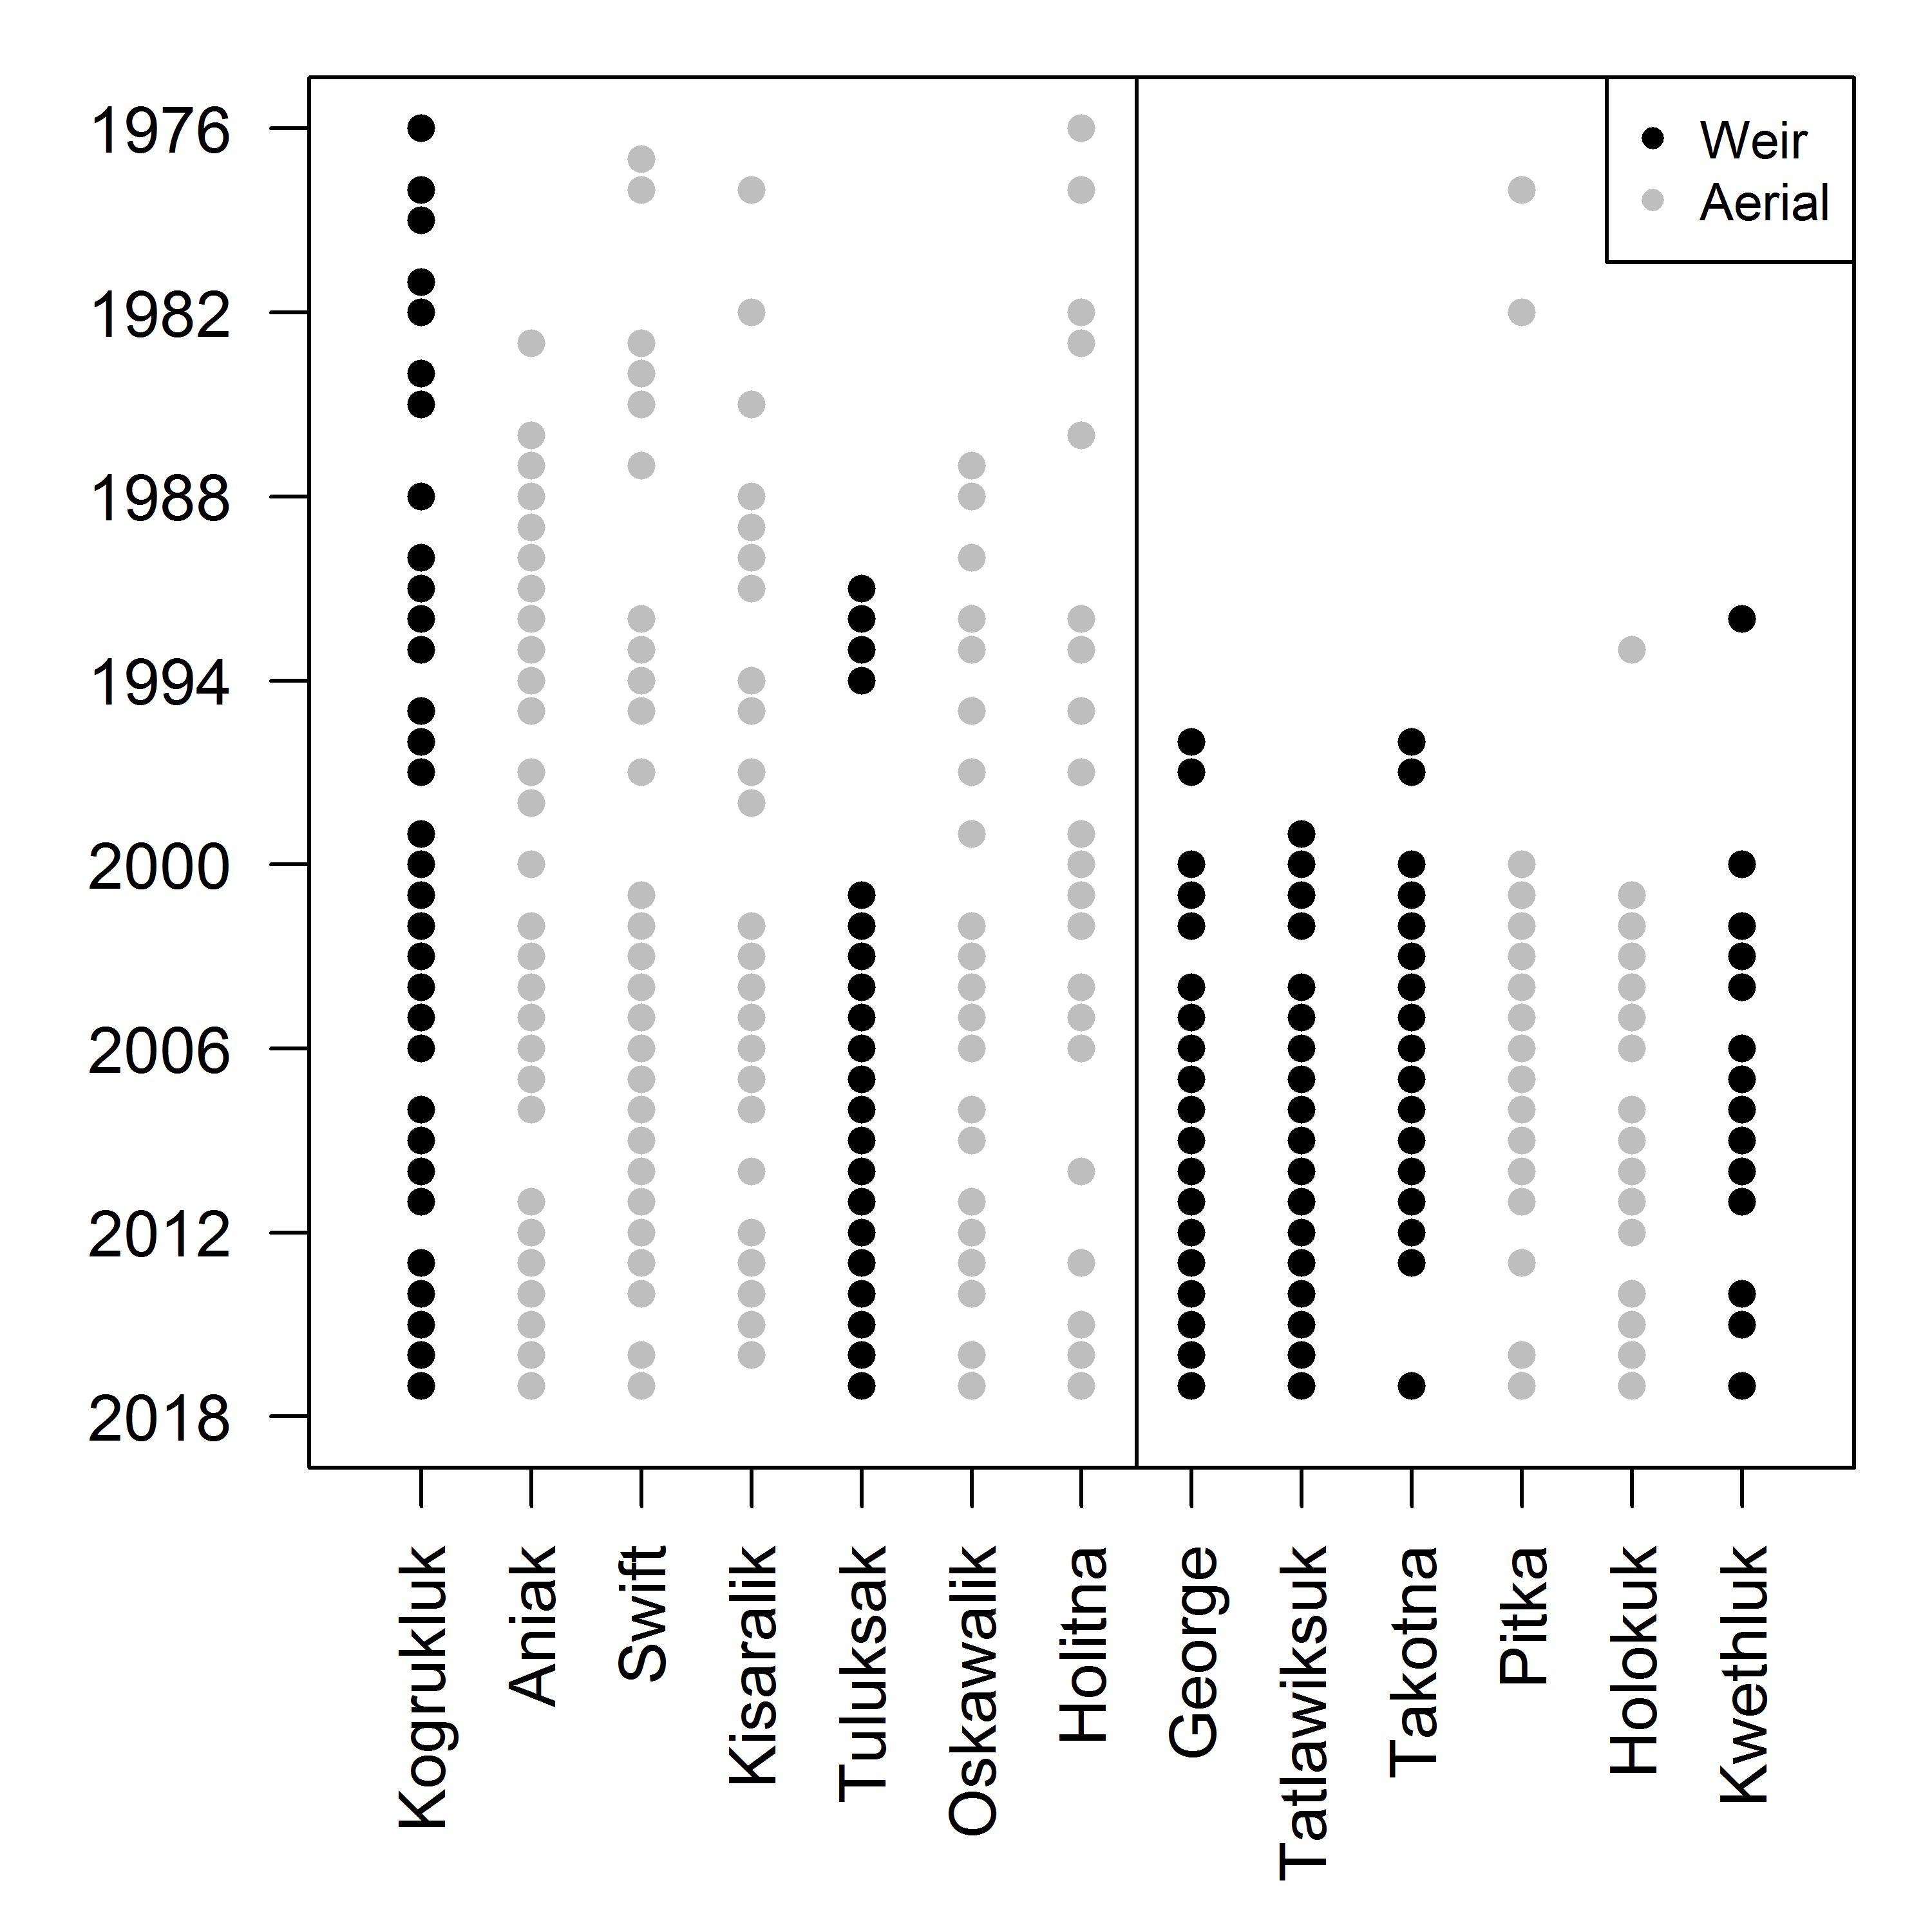
\includegraphics{img/Ch4/obs-freq.jpg}
  \caption{The frequency of escapement sampling for each substock sampled in the Kuskokwim River. Black points indicate years that were sampled for substocks monitored with a weir and grey points indicate years sampled for substocks monitored with aerial surveys. The vertical black line shows a break where > 50\% of the years were monitored for a stock.}
  \label{fig:obs-freq}
\end{figure}

\clearpage

\begin{figure}
  \centering
  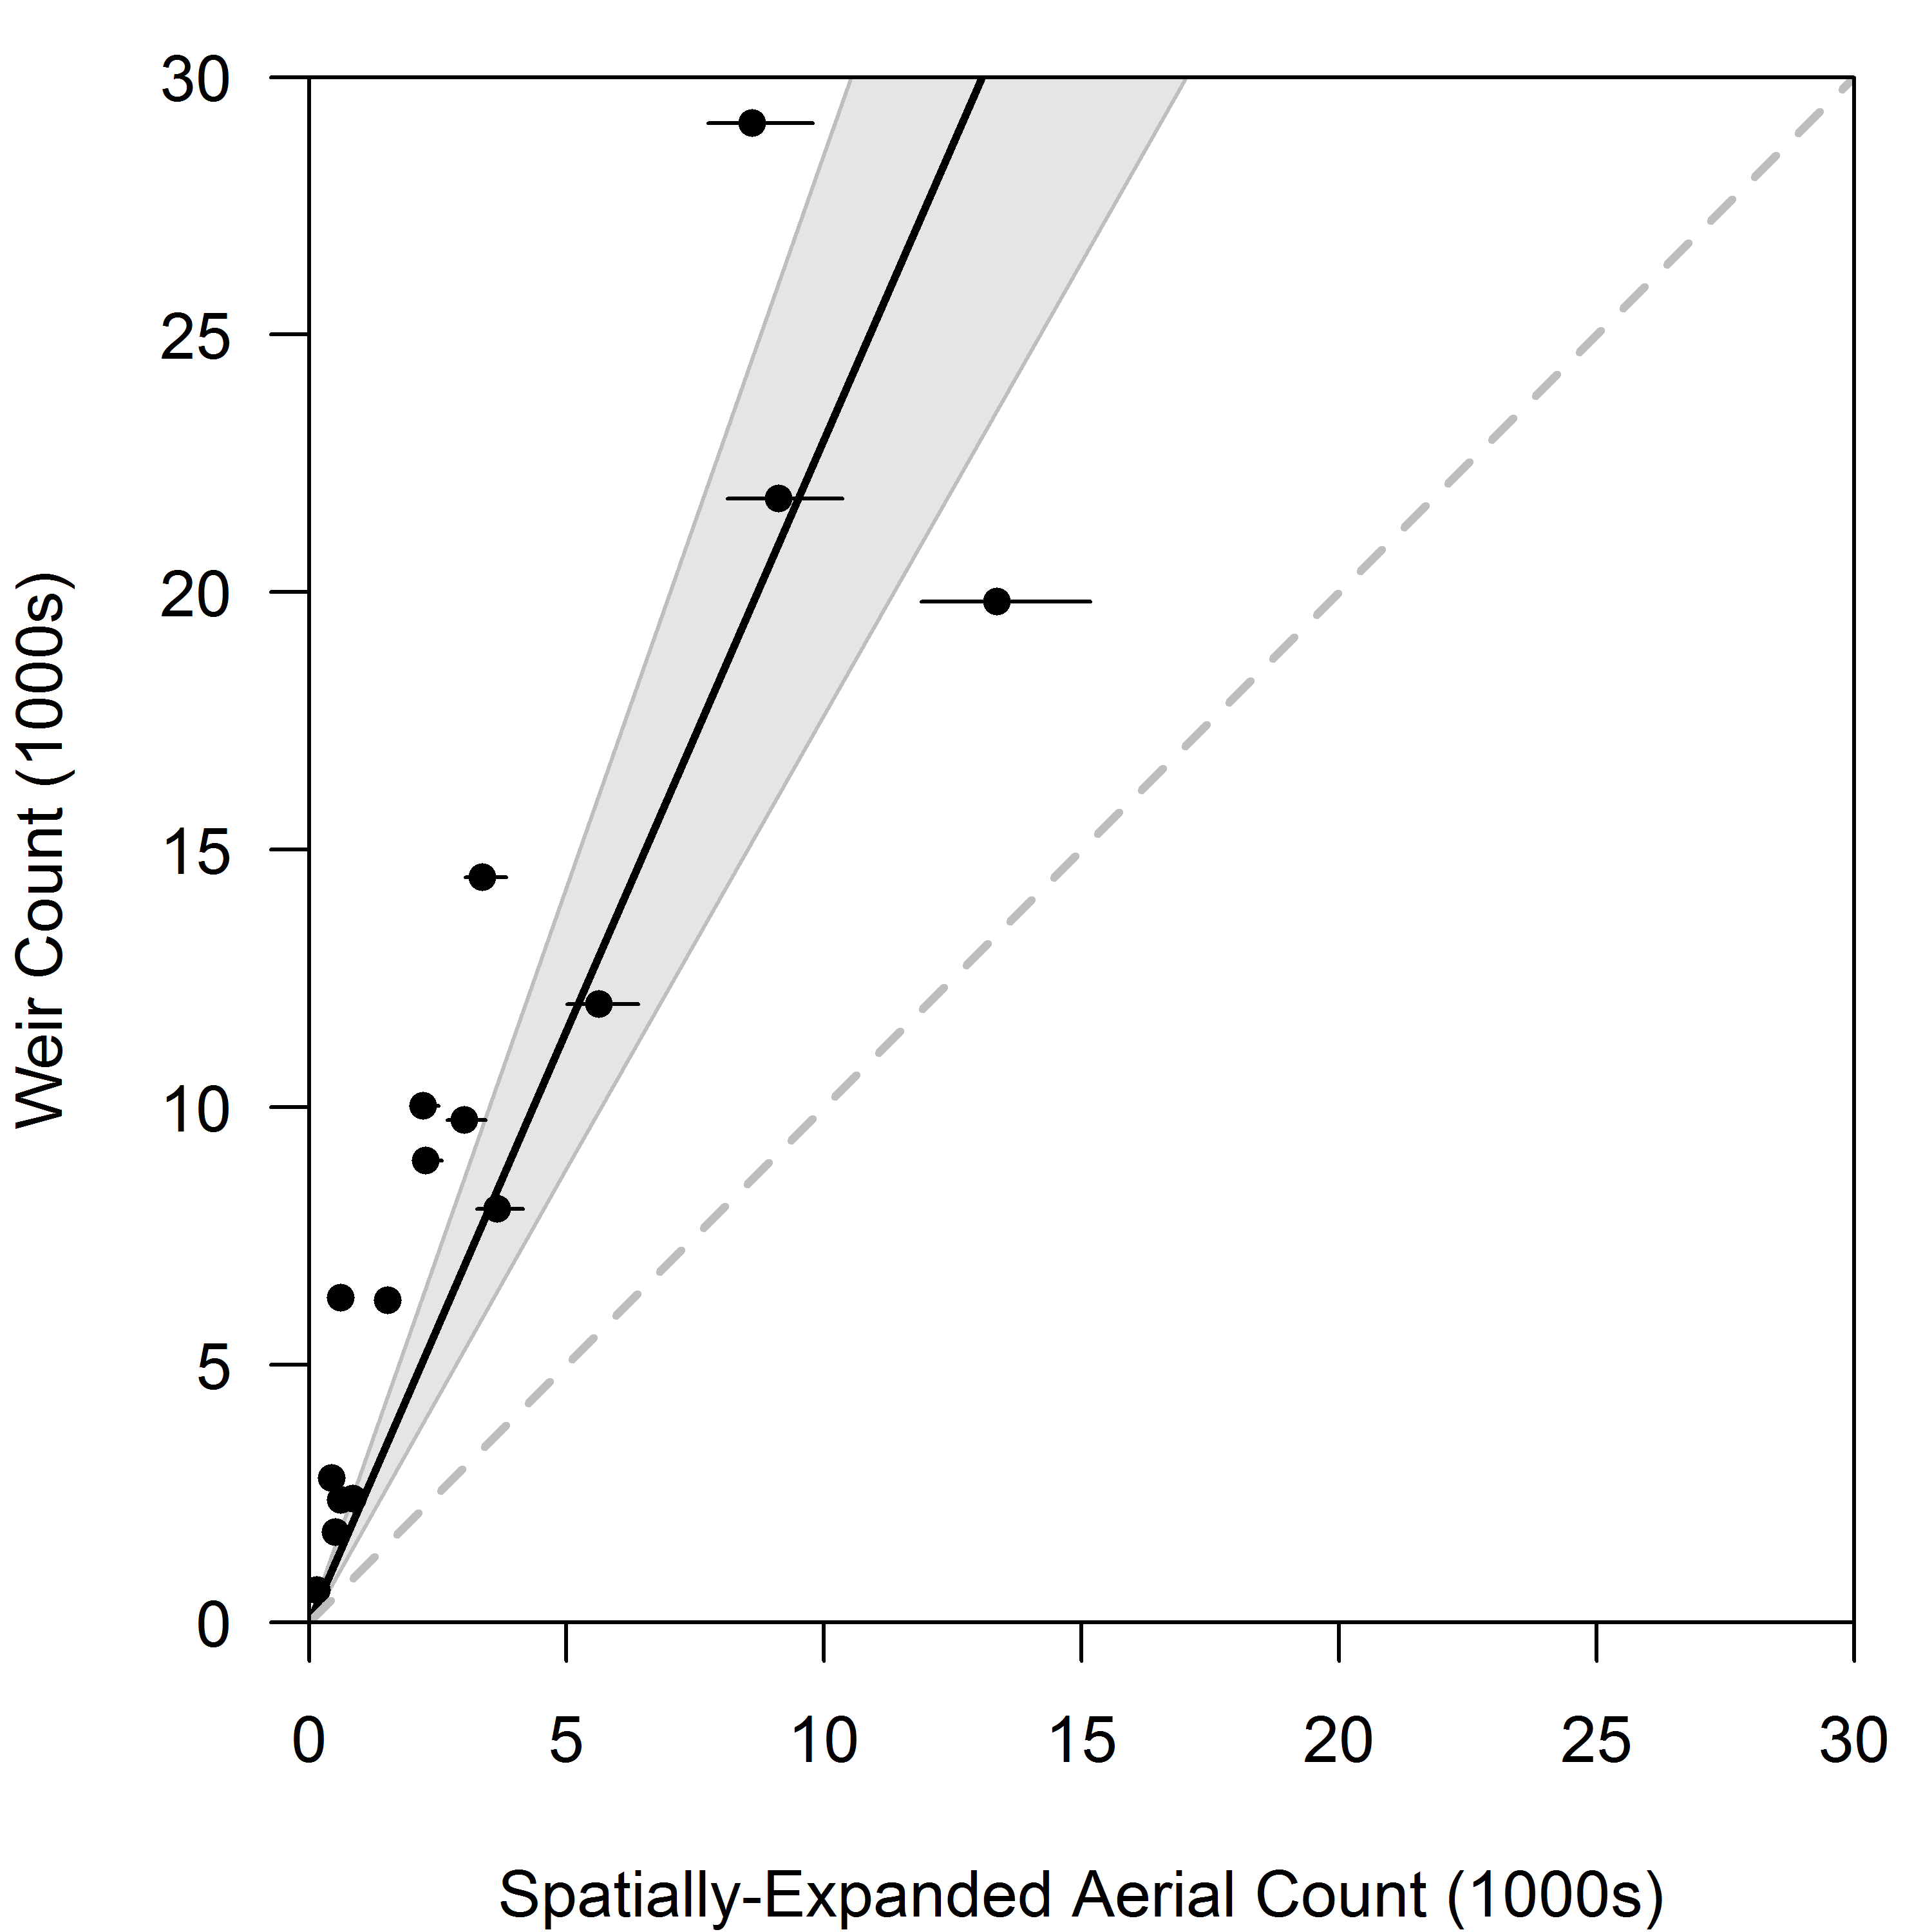
\includegraphics{img/Ch4/obs-correct.png}
  \caption{The relationship between spatially-expanded aerial survey estimates and weir counts during the same years and substocks as described by (\ref{eq:temp-expand1}). Notice the uncertainty expressed in the predictor variable; this was included in the analysis by incorporating both the spatial (Section \ref{spat-expansion}) and temporal (Section \ref{temp-expansion}) expansions in a single model fitted using Bayesian methods.}
  \label{fig:obs-correct}
\end{figure}

\clearpage

\begin{figure}
  \centering
  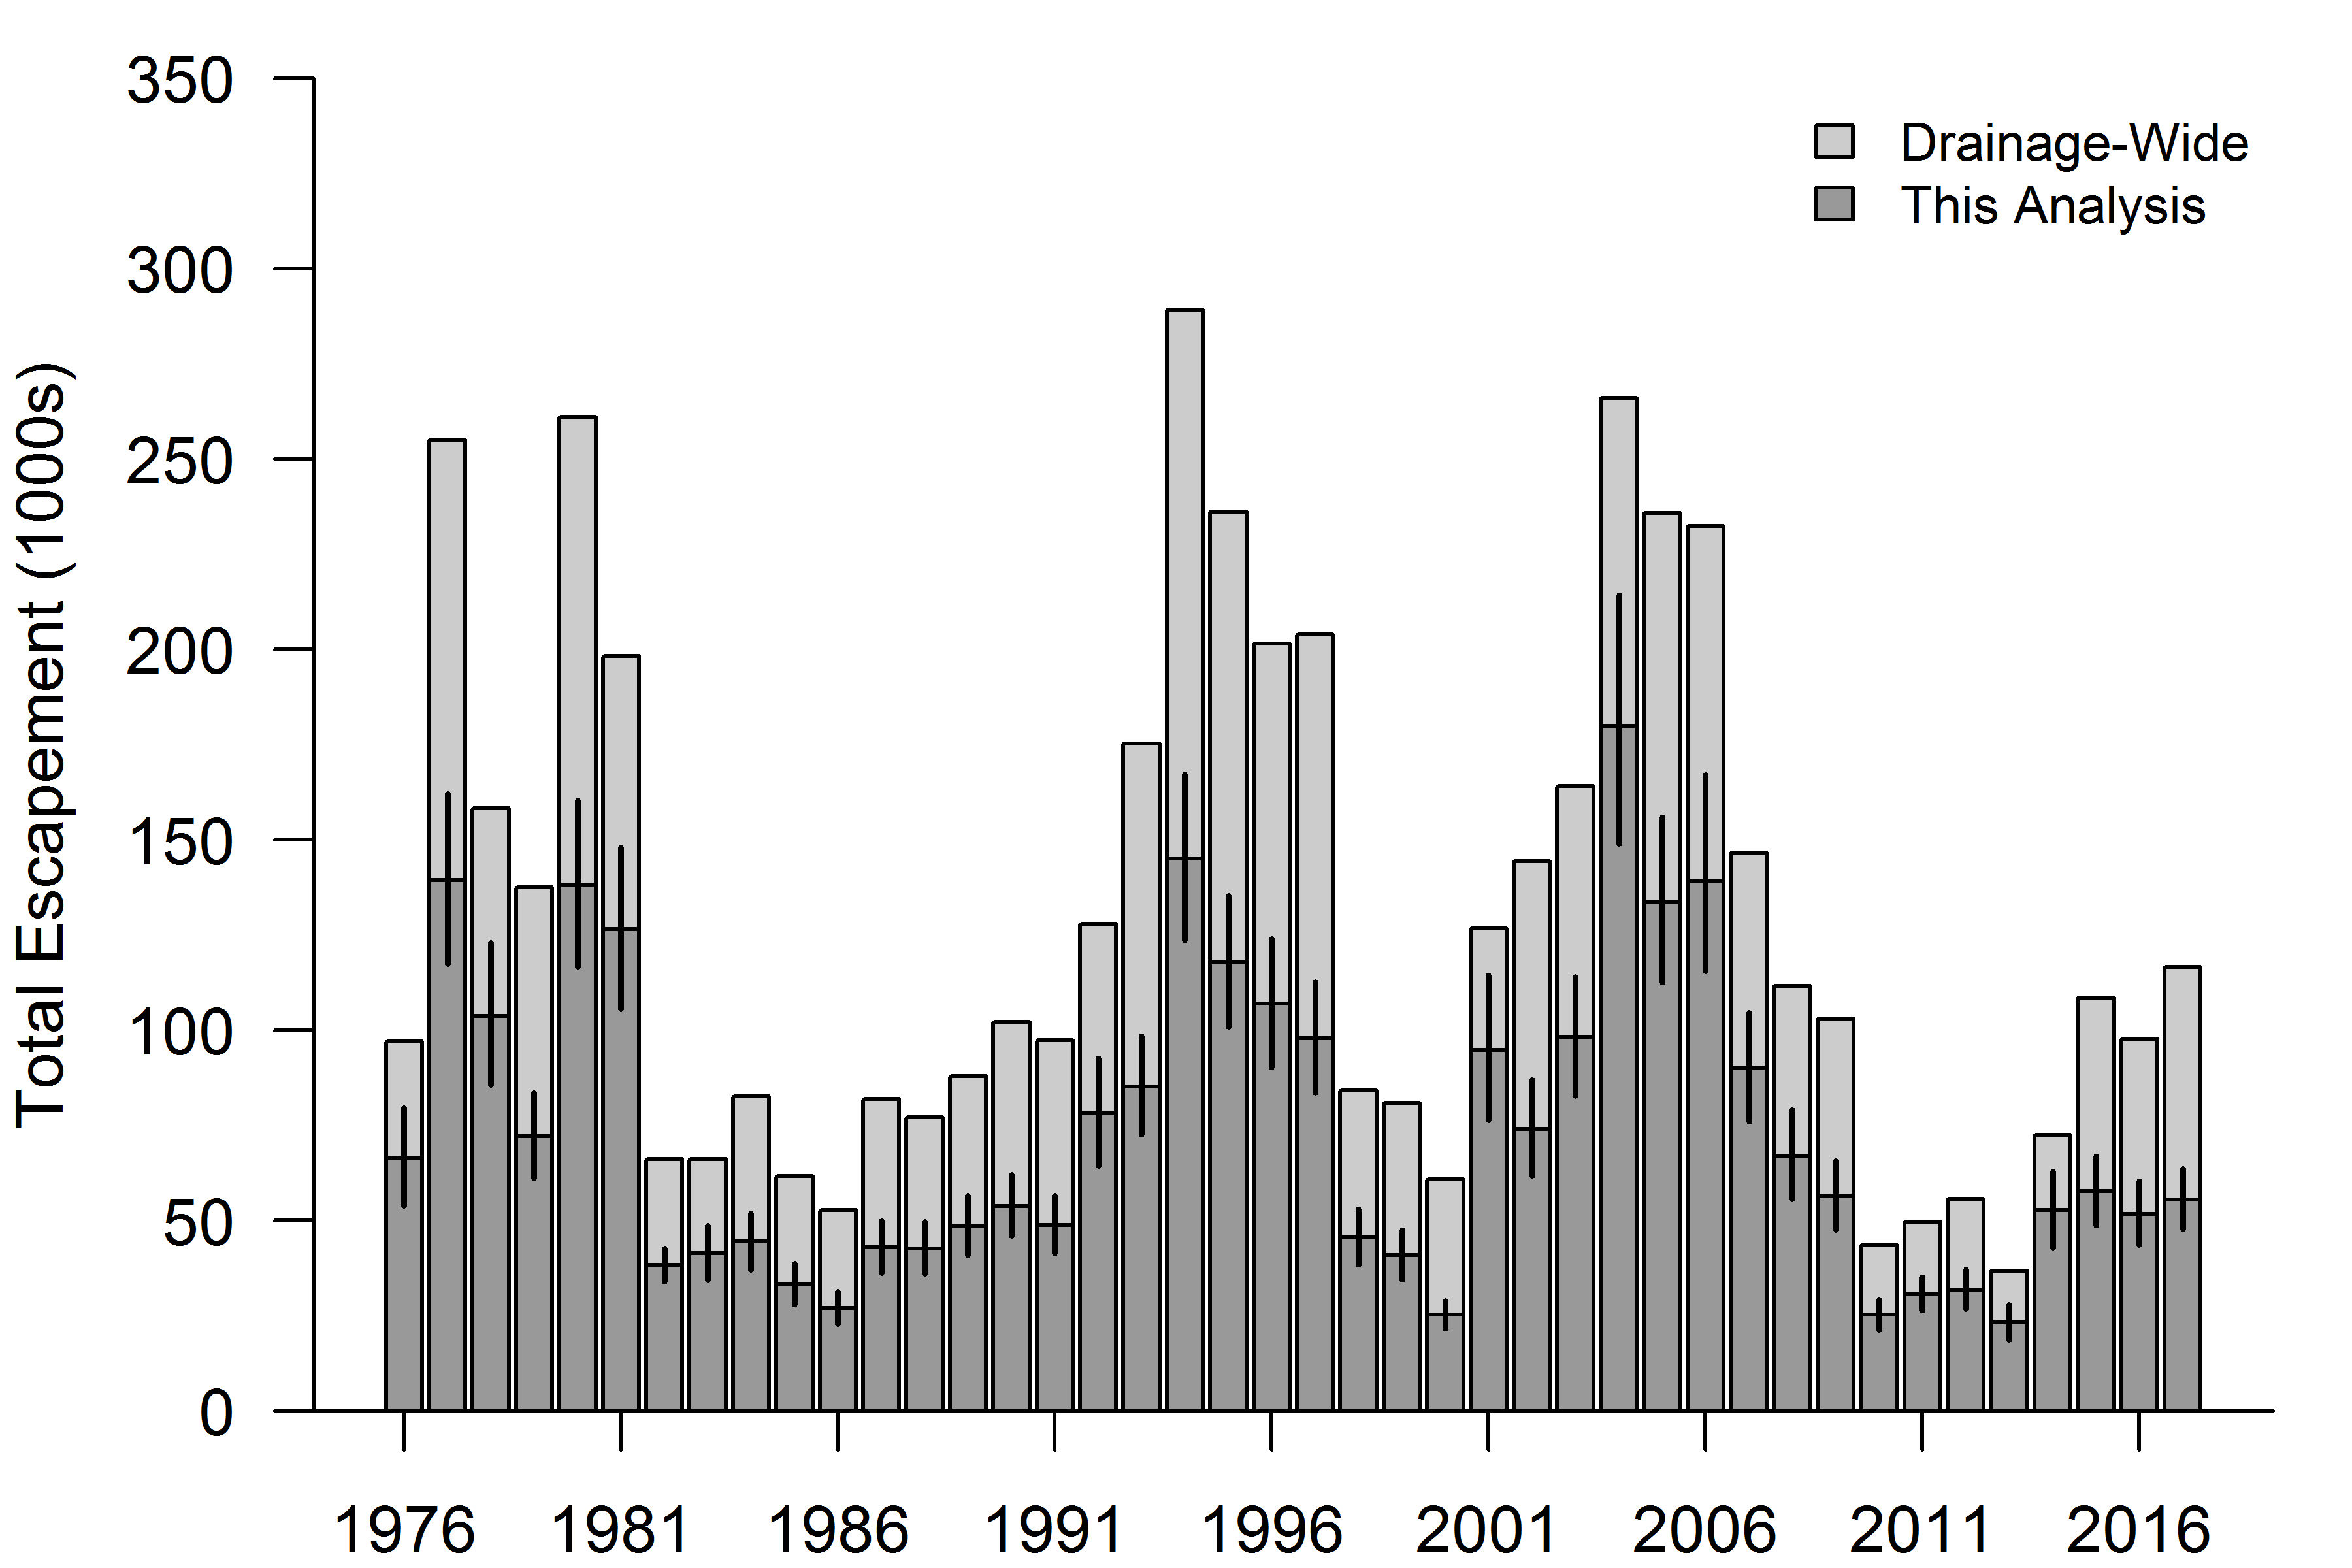
\includegraphics{img/Ch4/obs-fraction.png}
  \caption{Estimated Chinook salmon escapement for substocks within the Kuskokwim River drainage. ``Drainage-wide'' refers to the aggregate population estimates provided by a maximum likelihood run reconstruction model. ``This analysis'' refers to the estimated portion of the aggregate run included in this analysis (not all tributaries have been monitored).}
  \label{fig:obs-fraction}
\end{figure}

\chapter{Simulation of Substock- and Year-Specific Maturity
Schedules}\label{appendix-d}

\doublespacing

\noindent
In the operating model of the simulation-estimation component of Chapter
\ref{ch4}, maturity variability was modeled with more complexity than
assumed by the most complex estimation model. It was simulated to vary
on average by substock (i.e., some substocks would tend to mature at
younger or earlier ages). Additionally, brood-year specific random
maturity schedules were generated for each substock, though were
simulated to be highly synchronous among substocks. I was unaware of a
way to model such correlated dynamics using the Dirichlet random
process, so I generated it using a hierarchical linear modeling
approach. Note that some of the notation in this appendix uses symbols
with different meanings in the main text and other appendices.

\section{Single substock, single year
example}\label{single-substock-single-year-example}

\noindent
First, define a vector of \(n_a - 1\) coefficients:

\[
\boldsymbol{\gamma}=
  \begin{bmatrix}
    \gamma_{0} & \gamma_1 & \gamma_2
  \end{bmatrix}
\]

\noindent
and a design matrix with rows and columns equal to \(n_a - 1\):

\[
\mathbf{X}=
  \begin{bmatrix}
    1 & 0 & 0 \\
    1 & 1 & 0 \\
    1 & 0 & 1
  \end{bmatrix}
\]

\noindent
Then, combine them into a linear predictor on the logit scale:

\[\text{logit}(\boldsymbol{\psi}) = \mathbf{X}\boldsymbol{\gamma}\]

\noindent
The vector \(\boldsymbol{\psi}\) contains the probability of maturity at
each age, conditional on not having matured at any previous age for the
first \(n_a - 1\) possible ages-at-maturation. The elements of
\(\boldsymbol{\psi}\) can be converted to marginal probabilities of
maturiting at each age (elements of \(\boldsymbol{p}\)):

\[
  p_a = \left\{ \begin{array}{ll}
  \psi_a & \mbox{if $a = 1$} \\
  \psi_a(1 - \sum_{a=1}^{a-1} p_a) & \mbox{if 1 < $a$ < $n_a - 1$} \\
  1 - \sum_{a=1}^{a-1} p_a & \mbox{if $a = n_a$ } \\
  \end{array}
  \right. \\
\]

\noindent
These marginal probabilities can be then used to apportion recruitments
occurring from brood year \(y\) to the various calendar years of
observation \(t\).

\section{Extention to multiple substocks and
years}\label{extention-to-multiple-substocks-and-years}

\noindent
Alterations were made to the \(\gamma_0\) parameter to be specific to
each substock and year combination. Stock-level effects were randomly
sampled:

\[\varepsilon_{j} \sim \text{N}(0, \sigma_{j}),\]

\noindent
then brood year- and substock-specific random effects were sampled:

\[\varepsilon_{y,1:n_j} \sim \text{MVN}(\varepsilon_{1:n_j}, \Sigma_{y}),\]

\noindent
to obtain the year- and substock-specific parameter:

\[\gamma_{0,y,j} = \gamma_0 + \varepsilon_{y,j}.\]

The following parameter values were used: \(\gamma_0\) = -1.4,
\(\gamma_1\) = 1.4, \(\gamma_2\) = 4, and \(\sigma_{j}\) = 0.25. The
covariance matrix \(\Sigma_y\) was constructed with standard deviations
for each substock equal to 0.2 and correlation equal to 0.9. These
settings resulted in an average vector maturation probabilities of 0.2,
0.4, 0.37, and 0.03 for ages 4, 5, 6, and 7, respectively. An example is
shown in Figure \ref{fig:maturity-sim-fig}.

\begin{figure}
  \centering
  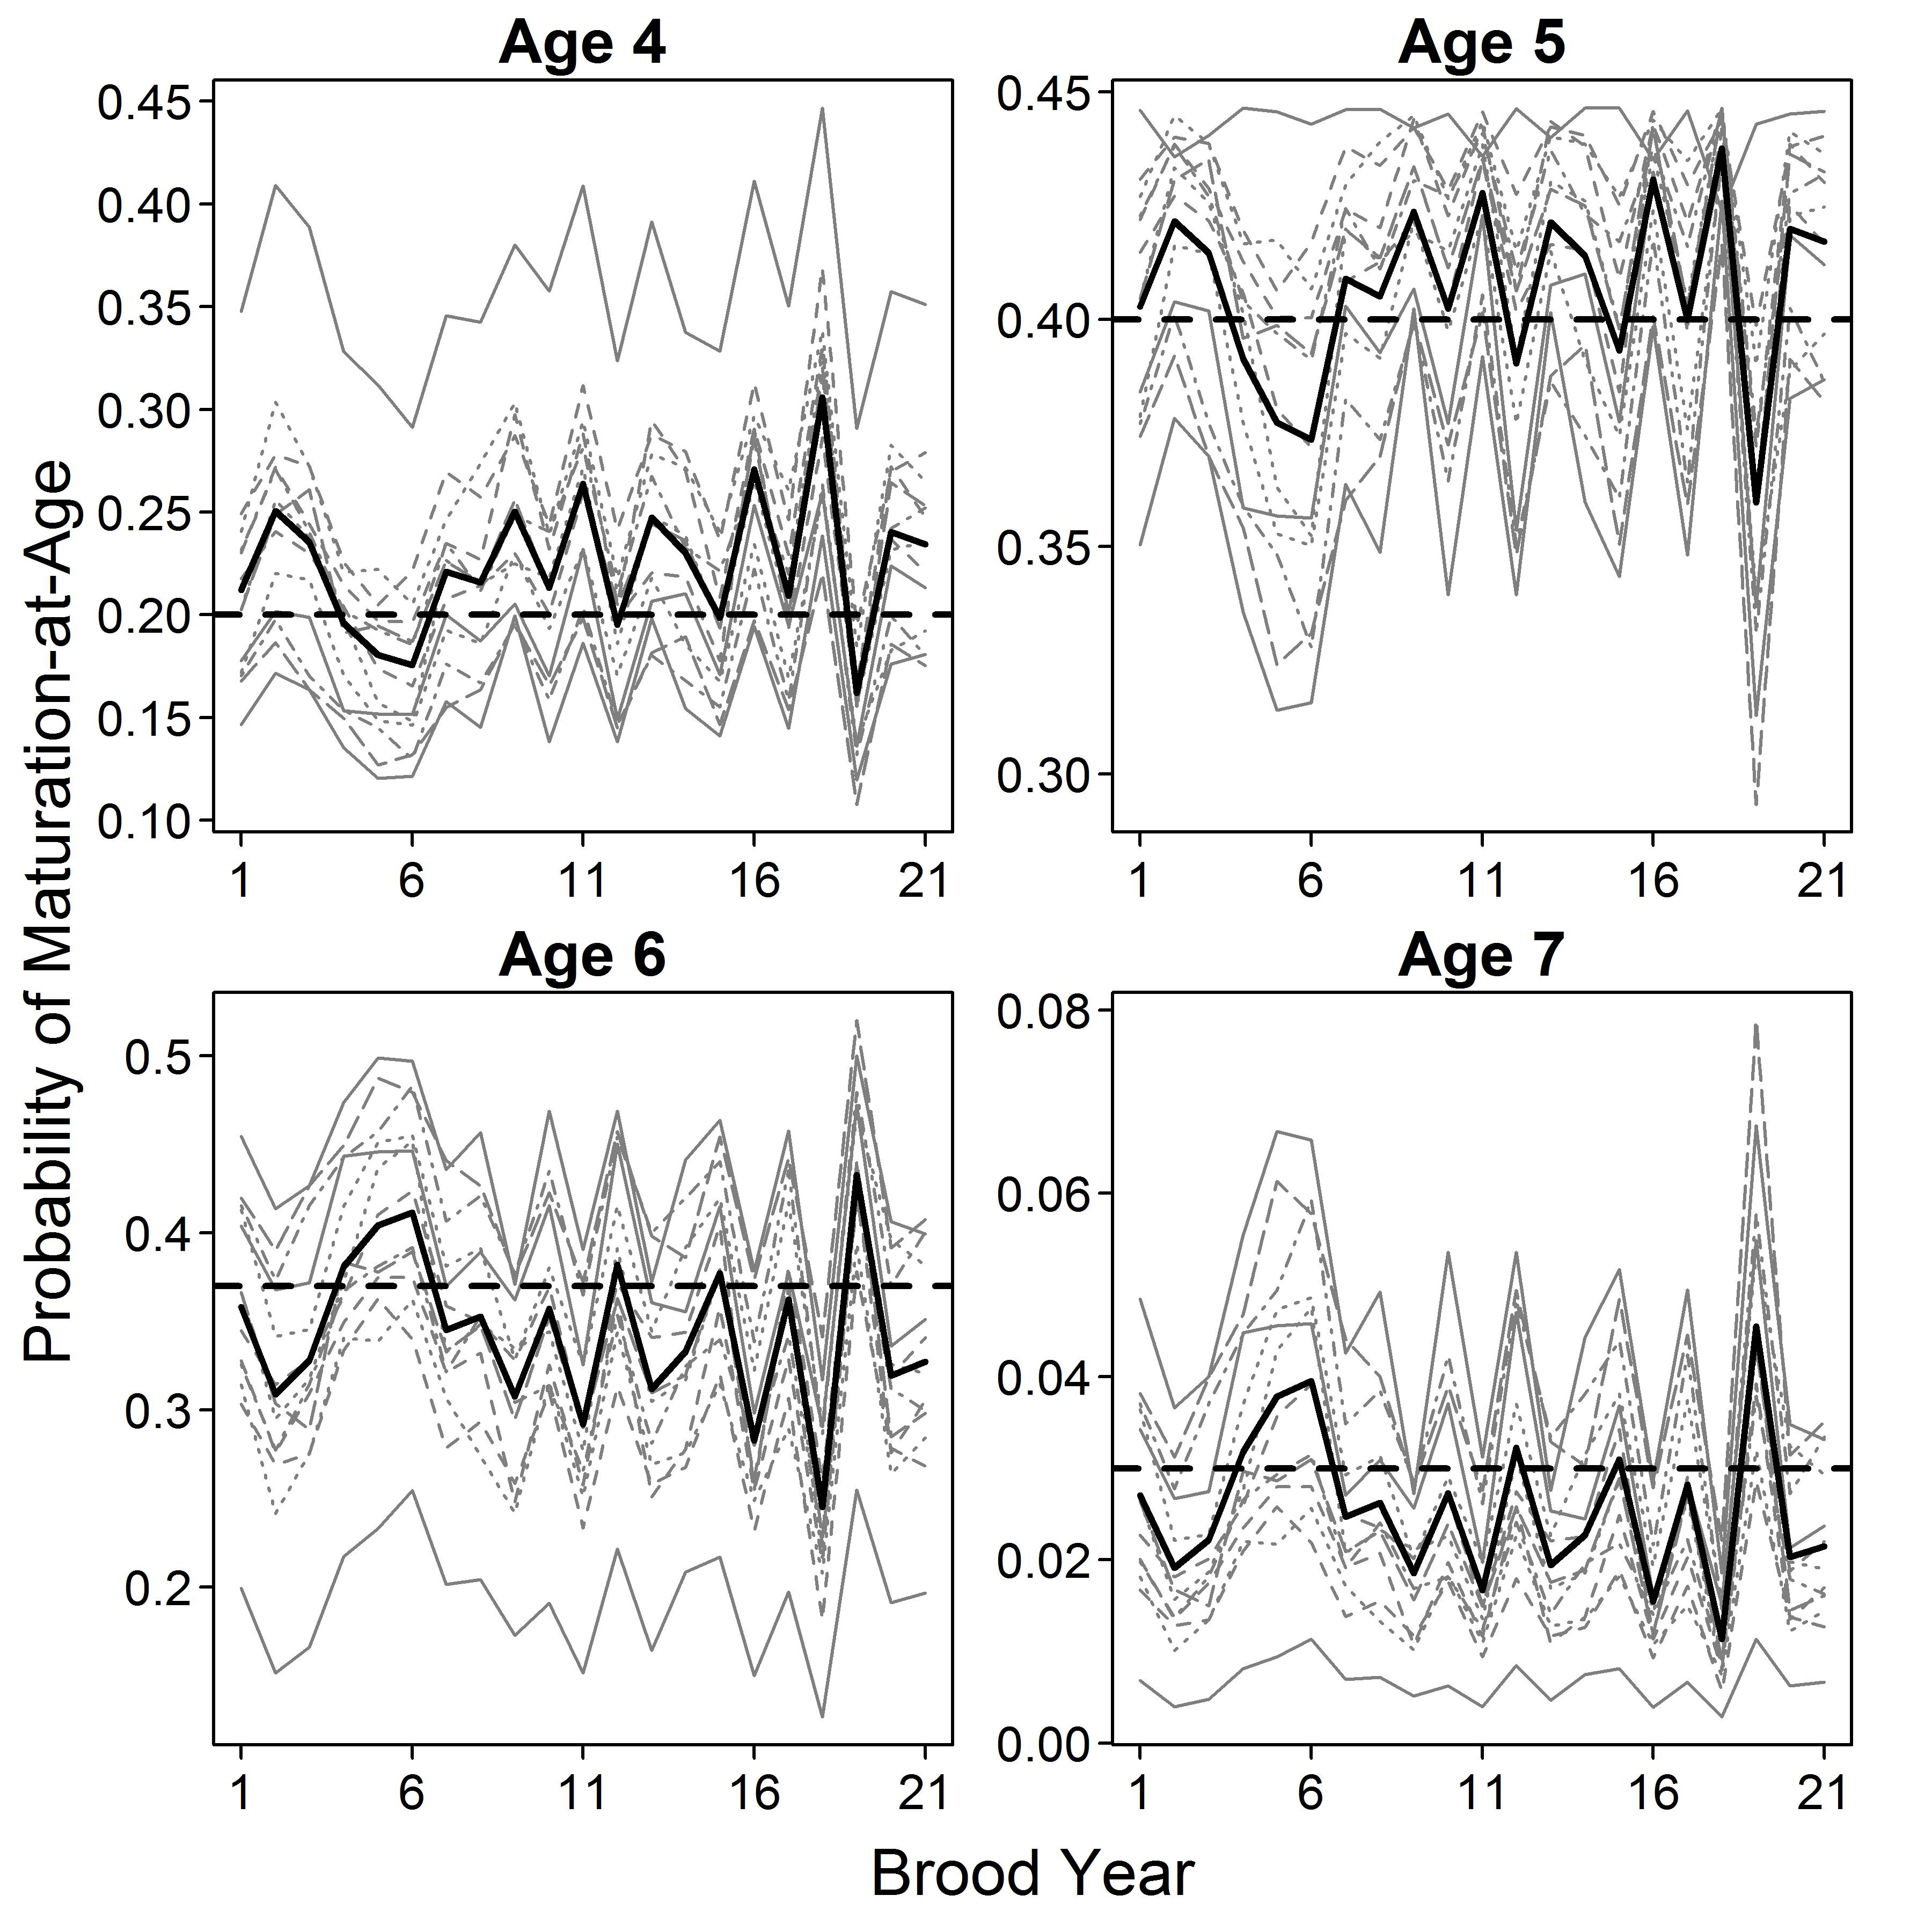
\includegraphics{img/Ch4/maturity-sim-fig.jpg}
  \caption{Simulated probability of maturation-at-age for 13 simulated substocks over time. The horizontal dashed line represents maturity without substock or year random effects and the black solid represents the average across substocks. Note the highly correlated patterns in year-specific variability.}
  \label{fig:maturity-sim-fig}
\end{figure}

\singlespacing

\bibliography{cites-without-doi.bib,cites-with-doi.bib}


\end{document}
